\documentclass[twoside]{book}

% Packages required by doxygen
\usepackage{fixltx2e}
\usepackage{calc}
\usepackage{doxygen}
\usepackage[export]{adjustbox} % also loads graphicx
\usepackage{graphicx}
\usepackage[utf8]{inputenc}
\usepackage{makeidx}
\usepackage{multicol}
\usepackage{multirow}
\PassOptionsToPackage{warn}{textcomp}
\usepackage{textcomp}
\usepackage[nointegrals]{wasysym}
\usepackage[table]{xcolor}

% Font selection
\usepackage[T1]{fontenc}
\usepackage[scaled=.90]{helvet}
\usepackage{courier}
\usepackage{amssymb}
\usepackage{sectsty}
\renewcommand{\familydefault}{\sfdefault}
\allsectionsfont{%
  \fontseries{bc}\selectfont%
  \color{darkgray}%
}
\renewcommand{\DoxyLabelFont}{%
  \fontseries{bc}\selectfont%
  \color{darkgray}%
}
\newcommand{\+}{\discretionary{\mbox{\scriptsize$\hookleftarrow$}}{}{}}

% Page & text layout
\usepackage{geometry}
\geometry{%
  a4paper,%
  top=2.5cm,%
  bottom=2.5cm,%
  left=2.5cm,%
  right=2.5cm%
}
\tolerance=750
\hfuzz=15pt
\hbadness=750
\setlength{\emergencystretch}{15pt}
\setlength{\parindent}{0cm}
\setlength{\parskip}{0.2cm}
\makeatletter
\renewcommand{\paragraph}{%
  \@startsection{paragraph}{4}{0ex}{-1.0ex}{1.0ex}{%
    \normalfont\normalsize\bfseries\SS@parafont%
  }%
}
\renewcommand{\subparagraph}{%
  \@startsection{subparagraph}{5}{0ex}{-1.0ex}{1.0ex}{%
    \normalfont\normalsize\bfseries\SS@subparafont%
  }%
}
\makeatother

% Headers & footers
\usepackage{fancyhdr}
\pagestyle{fancyplain}
\fancyhead[LE]{\fancyplain{}{\bfseries\thepage}}
\fancyhead[CE]{\fancyplain{}{}}
\fancyhead[RE]{\fancyplain{}{\bfseries\leftmark}}
\fancyhead[LO]{\fancyplain{}{\bfseries\rightmark}}
\fancyhead[CO]{\fancyplain{}{}}
\fancyhead[RO]{\fancyplain{}{\bfseries\thepage}}
\fancyfoot[LE]{\fancyplain{}{}}
\fancyfoot[CE]{\fancyplain{}{}}
\fancyfoot[RE]{\fancyplain{}{\bfseries\scriptsize Generated on Mon Feb 8 2016 17\+:45\+:40 for W\+D\+Lib\+\_\+\+Arduino by Doxygen }}
\fancyfoot[LO]{\fancyplain{}{\bfseries\scriptsize Generated on Mon Feb 8 2016 17\+:45\+:40 for W\+D\+Lib\+\_\+\+Arduino by Doxygen }}
\fancyfoot[CO]{\fancyplain{}{}}
\fancyfoot[RO]{\fancyplain{}{}}
\renewcommand{\footrulewidth}{0.4pt}
\renewcommand{\chaptermark}[1]{%
  \markboth{#1}{}%
}
\renewcommand{\sectionmark}[1]{%
  \markright{\thesection\ #1}%
}

% Indices & bibliography
\usepackage{natbib}
\usepackage[titles]{tocloft}
\setcounter{tocdepth}{3}
\setcounter{secnumdepth}{5}
\makeindex

% Hyperlinks (required, but should be loaded last)
\usepackage{ifpdf}
\ifpdf
  \usepackage[pdftex,pagebackref=true]{hyperref}
\else
  \usepackage[ps2pdf,pagebackref=true]{hyperref}
\fi
\hypersetup{%
  colorlinks=true,%
  linkcolor=blue,%
  citecolor=blue,%
  unicode%
}

% Custom commands
\newcommand{\clearemptydoublepage}{%
  \newpage{\pagestyle{empty}\cleardoublepage}%
}


%===== C O N T E N T S =====

\begin{document}

% Titlepage & ToC
\hypersetup{pageanchor=false,
             bookmarks=true,
             bookmarksnumbered=true,
             pdfencoding=unicode
            }
\pagenumbering{roman}
\begin{titlepage}
\vspace*{7cm}
\begin{center}%
{\Large W\+D\+Lib\+\_\+\+Arduino }\\
\vspace*{1cm}
{\large Generated by Doxygen 1.8.10}\\
\vspace*{0.5cm}
{\small Mon Feb 8 2016 17:45:40}\\
\end{center}
\end{titlepage}
\clearemptydoublepage
\tableofcontents
\clearemptydoublepage
\pagenumbering{arabic}
\hypersetup{pageanchor=true}

%--- Begin generated contents ---
\chapter{W\+D\+Lib\+\_\+\+Arduino}
\label{index}\hypertarget{index}{}This is a collection of usefull functions and classes for the Arduino platorm.

Home Page\+: \href{http://busyducks.com/}{\tt http\+://busyducks.\+com/}

Graph Plotting\+:
\begin{DoxyItemize}
\item Supports sending G\+N\+U\+Plot commands to create graphs of your data.
\item \#include $<$\hyperlink{_serial_graph_8h}{Serial\+Graph.\+h}$>$
\item \#include $<$\hyperlink{_g_n_u_plot_8h}{G\+N\+U\+Plot.\+h}$>$
\item see \hyperlink{class_serial_graph}{Serial\+Graph} as the base class.
\item see \hyperlink{struct_line_apperance}{Line\+Apperance} for changing the apperance of a series. Included color schemes suitable for graphing.
\begin{DoxyItemize}
\item Strong, but balanced, colors for unrelated catagories \hyperlink{_line_apperance_8h_a1e42ce190c01f4415b1ea96e3f113c84}{Categorical\+Scheme\+Strong}
\item Balanced colors for graphing \hyperlink{_line_apperance_8h_a6d48f70f76f6e9d41e4272b04dff1008}{Graph\+Colors\+Scheme\+Grey\+Scale}, \hyperlink{_line_apperance_8h_a277e168f3720b3d07131d9d402f28f33}{Graph\+Colors\+Scheme\+Red\+Scale}, \hyperlink{_line_apperance_8h_a0ab80737f9ec4bde245b67fd27a53d36}{Graph\+Colors\+Scheme\+Green\+Scale}, \hyperlink{_line_apperance_8h_a948426d1c597f9820a092fc49737bd7f}{Graph\+Colors\+Scheme\+Blue\+Scale}, \hyperlink{_line_apperance_8h_a73a0c1e1e60774d861f1887c24078ee9}{Graph\+Colors\+Scheme\+Orange\+Scale}, \hyperlink{_line_apperance_8h_a8462197caad1bdc2b174b46899e68793}{Graph\+Colors\+Scheme\+Purple\+Scale}
\item Spectral colors for graphing on a white background \hyperlink{_line_apperance_8h_a250826c1d27d3626eb24afa95310041f}{Graph\+Colors\+Scheme\+Spectral}
\item Colors for colorblind compatability \hyperlink{_line_apperance_8h_abc59bc8bf0930be7e1ced4a6ca602688}{Color\+Blind\+Safe}
\end{DoxyItemize}
\end{DoxyItemize}String validation
\begin{DoxyItemize}
\item For validating input strings and external data.
\item \#include $<$\hyperlink{_string_validation_8h}{String\+Validation.\+h}$>$
\item Allows filering of against a combination of flags, see String\+Validation\+Rules.
\item Can operate in three modes\+: inplace, copy to another buffer, allocate a new buffer.
\item {\itshape Not} intended to be a \char`\"{}security grade\char`\"{} validation to protect against various attacks.
\end{DoxyItemize}Bit Arithmatic
\begin{DoxyItemize}
\item Helpers for dealing with bits and bytes
\item \#include $<$\hyperlink{_bit_arithmatic_8h}{Bit\+Arithmatic.\+h}$>$
\item \hyperlink{_bit_arithmatic_8h_aabbf277315ff3b8310a7741925b56bc7}{set\+Bits}(...) Stores a n bit number at given bit position
\item \hyperlink{_bit_arithmatic_8h_a1131897261971e497cf6a4a83476fcdc}{get\+Bits}(...) Gets a n bit number at given bit position
\item \hyperlink{_bit_arithmatic_8h_a07b9d02b23a7b5526117bd66036cc516}{print\+Hex\+Byte} \hyperlink{_bit_arithmatic_8h_a2b7e446093fa0d1d250eea3d908ea28f}{print\+Hex\+Int16} \hyperlink{_bit_arithmatic_8h_af2a2e4872a45c5012fa0a63053e63f20}{print\+Hex\+Int24} \hyperlink{_bit_arithmatic_8h_ae6e1c4ca3c19e4a1e97ade02f5c7667b}{print\+Hex\+Int32} output numbers as hex, with leading 0\textquotesingle{}s
\item \hyperlink{_bit_arithmatic_8h_a1e55823ca5d6c66eba53036134820785}{bytes\+To32bit} \hyperlink{_bit_arithmatic_8h_aa0bec3f30220610f221e46f327d13bf9}{bytes\+To16bit} Assembles integers from bytes.
\end{DoxyItemize}

General Helpers
\begin{DoxyItemize}
\item \#include $<$\hyperlink{_sanity_8h}{Sanity.\+h}$>$
\item \+::\+Arduino\+Baud\+Rates
\item A few methods that fill the gap between \+\_\+\+\_\+\+Flash\+String\+Helper and general strings.
\begin{DoxyItemize}
\item eg. strcmp(my\+Str, F(\char`\"{}start\char`\"{})) is now possible.
\end{DoxyItemize}
\end{DoxyItemize}Capture Print
\begin{DoxyItemize}
\item \#include $<$\hyperlink{_capture_print_8h}{Capture\+Print.\+h}$>$
\item Implements the Arduino Print class, re-\/directing all output to a buffer.
\item Processes Print data one line at a time
\item Great for\+:
\begin{DoxyItemize}
\item Grep like activites on lines of output.
\item Employing the powerful Print functionality to format strings.
\item Adding checksum calculations to output text.
\item Unit testing print functions.
\item Capturing stream output and sending to multiple other streams.
\end{DoxyItemize}
\end{DoxyItemize}
\chapter{Hierarchical Index}
\section{Class Hierarchy}
This inheritance list is sorted roughly, but not completely, alphabetically\+:\begin{DoxyCompactList}
\item \contentsline{section}{Line\+Apperance}{\pageref{struct_line_apperance}}{}
\item Print\begin{DoxyCompactList}
\item \contentsline{section}{Capture\+Print}{\pageref{class_capture_print}}{}
\item \contentsline{section}{Pre\+Print}{\pageref{class_pre_print}}{}
\end{DoxyCompactList}
\item \contentsline{section}{Serial\+Graph}{\pageref{class_serial_graph}}{}
\begin{DoxyCompactList}
\item \contentsline{section}{G\+N\+U\+Plot\+Base}{\pageref{class_g_n_u_plot_base}}{}
\begin{DoxyCompactList}
\item \contentsline{section}{G\+N\+U\+Plot\+Bar\+Graph}{\pageref{class_g_n_u_plot_bar_graph}}{}
\item \contentsline{section}{G\+N\+U\+Plot\+X\+Y\+Graph\+Base}{\pageref{class_g_n_u_plot_x_y_graph_base}}{}
\begin{DoxyCompactList}
\item \contentsline{section}{G\+N\+U\+Plot\+Line\+Graph}{\pageref{class_g_n_u_plot_line_graph}}{}
\item \contentsline{section}{G\+N\+U\+Plot\+Point\+Graph}{\pageref{class_g_n_u_plot_point_graph}}{}
\end{DoxyCompactList}
\end{DoxyCompactList}
\end{DoxyCompactList}
\end{DoxyCompactList}

\chapter{Class Index}
\section{Class List}
Here are the classes, structs, unions and interfaces with brief descriptions\+:\begin{DoxyCompactList}
\item\contentsline{section}{\hyperlink{class_capture_print}{Capture\+Print} }{\pageref{class_capture_print}}{}
\item\contentsline{section}{\hyperlink{class_g_n_u_plot_bar_graph}{G\+N\+U\+Plot\+Bar\+Graph} }{\pageref{class_g_n_u_plot_bar_graph}}{}
\item\contentsline{section}{\hyperlink{class_g_n_u_plot_base}{G\+N\+U\+Plot\+Base} }{\pageref{class_g_n_u_plot_base}}{}
\item\contentsline{section}{\hyperlink{class_g_n_u_plot_line_graph}{G\+N\+U\+Plot\+Line\+Graph} }{\pageref{class_g_n_u_plot_line_graph}}{}
\item\contentsline{section}{\hyperlink{class_g_n_u_plot_point_graph}{G\+N\+U\+Plot\+Point\+Graph} }{\pageref{class_g_n_u_plot_point_graph}}{}
\item\contentsline{section}{\hyperlink{class_g_n_u_plot_x_y_graph_base}{G\+N\+U\+Plot\+X\+Y\+Graph\+Base} }{\pageref{class_g_n_u_plot_x_y_graph_base}}{}
\item\contentsline{section}{\hyperlink{struct_line_apperance}{Line\+Apperance} }{\pageref{struct_line_apperance}}{}
\item\contentsline{section}{\hyperlink{class_pre_print}{Pre\+Print} }{\pageref{class_pre_print}}{}
\item\contentsline{section}{\hyperlink{class_serial_graph}{Serial\+Graph} }{\pageref{class_serial_graph}}{}
\end{DoxyCompactList}

\chapter{File Index}
\section{File List}
Here is a list of all files with brief descriptions\+:\begin{DoxyCompactList}
\item\contentsline{section}{W\+D\+Arduino\+Lib/src/\hyperlink{_bit_arithmatic_8cpp}{Bit\+Arithmatic.\+cpp} }{\pageref{_bit_arithmatic_8cpp}}{}
\item\contentsline{section}{W\+D\+Arduino\+Lib/src/\hyperlink{_bit_arithmatic_8h}{Bit\+Arithmatic.\+h} }{\pageref{_bit_arithmatic_8h}}{}
\item\contentsline{section}{W\+D\+Arduino\+Lib/src/\hyperlink{_capture_print_8cpp}{Capture\+Print.\+cpp} }{\pageref{_capture_print_8cpp}}{}
\item\contentsline{section}{W\+D\+Arduino\+Lib/src/\hyperlink{_capture_print_8h}{Capture\+Print.\+h} \\*\hyperlink{class_capture_print}{Capture\+Print} classe }{\pageref{_capture_print_8h}}{}
\item\contentsline{section}{W\+D\+Arduino\+Lib/src/\hyperlink{_cross_compile_8cpp}{Cross\+Compile.\+cpp} }{\pageref{_cross_compile_8cpp}}{}
\item\contentsline{section}{W\+D\+Arduino\+Lib/src/\hyperlink{_cross_compile_8h}{Cross\+Compile.\+h} }{\pageref{_cross_compile_8h}}{}
\item\contentsline{section}{W\+D\+Arduino\+Lib/src/\hyperlink{_g_n_u_plot_8cpp}{G\+N\+U\+Plot.\+cpp} }{\pageref{_g_n_u_plot_8cpp}}{}
\item\contentsline{section}{W\+D\+Arduino\+Lib/src/\hyperlink{_g_n_u_plot_8h}{G\+N\+U\+Plot.\+h} \\*G\+N\+Uplot interface classes }{\pageref{_g_n_u_plot_8h}}{}
\item\contentsline{section}{W\+D\+Arduino\+Lib/src/\hyperlink{_line_apperance_8cpp}{Line\+Apperance.\+cpp} }{\pageref{_line_apperance_8cpp}}{}
\item\contentsline{section}{W\+D\+Arduino\+Lib/src/\hyperlink{_line_apperance_8h}{Line\+Apperance.\+h} }{\pageref{_line_apperance_8h}}{}
\item\contentsline{section}{W\+D\+Arduino\+Lib/src/\hyperlink{_pre_print_8cpp}{Pre\+Print.\+cpp} }{\pageref{_pre_print_8cpp}}{}
\item\contentsline{section}{W\+D\+Arduino\+Lib/src/\hyperlink{_pre_print_8h}{Pre\+Print.\+h} \\*\hyperlink{class_pre_print}{Pre\+Print} class }{\pageref{_pre_print_8h}}{}
\item\contentsline{section}{W\+D\+Arduino\+Lib/src/\hyperlink{_sanity_8cpp}{Sanity.\+cpp} }{\pageref{_sanity_8cpp}}{}
\item\contentsline{section}{W\+D\+Arduino\+Lib/src/\hyperlink{_sanity_8h}{Sanity.\+h} }{\pageref{_sanity_8h}}{}
\item\contentsline{section}{W\+D\+Arduino\+Lib/src/\hyperlink{_serial_graph_8cpp}{Serial\+Graph.\+cpp} }{\pageref{_serial_graph_8cpp}}{}
\item\contentsline{section}{W\+D\+Arduino\+Lib/src/\hyperlink{_serial_graph_8h}{Serial\+Graph.\+h} }{\pageref{_serial_graph_8h}}{}
\item\contentsline{section}{W\+D\+Arduino\+Lib/src/\hyperlink{_string_validation_8cpp}{String\+Validation.\+cpp} }{\pageref{_string_validation_8cpp}}{}
\item\contentsline{section}{W\+D\+Arduino\+Lib/src/\hyperlink{_string_validation_8h}{String\+Validation.\+h} }{\pageref{_string_validation_8h}}{}
\item\contentsline{section}{W\+D\+Arduino\+Lib/src/\hyperlink{_w_d_arduino_lib___unit_tests_8cpp}{W\+D\+Arduino\+Lib\+\_\+\+Unit\+Tests.\+cpp} }{\pageref{_w_d_arduino_lib___unit_tests_8cpp}}{}
\item\contentsline{section}{W\+D\+Arduino\+Lib/src/\hyperlink{_w_d_arduino_lib___unit_tests_8h}{W\+D\+Arduino\+Lib\+\_\+\+Unit\+Tests.\+h} }{\pageref{_w_d_arduino_lib___unit_tests_8h}}{}
\end{DoxyCompactList}

\chapter{Class Documentation}
\hypertarget{class_capture_print}{}\section{Capture\+Print Class Reference}
\label{class_capture_print}\index{Capture\+Print@{Capture\+Print}}


{\ttfamily \#include $<$Capture\+Print.\+h$>$}

Inheritance diagram for Capture\+Print\+:\begin{figure}[H]
\begin{center}
\leavevmode
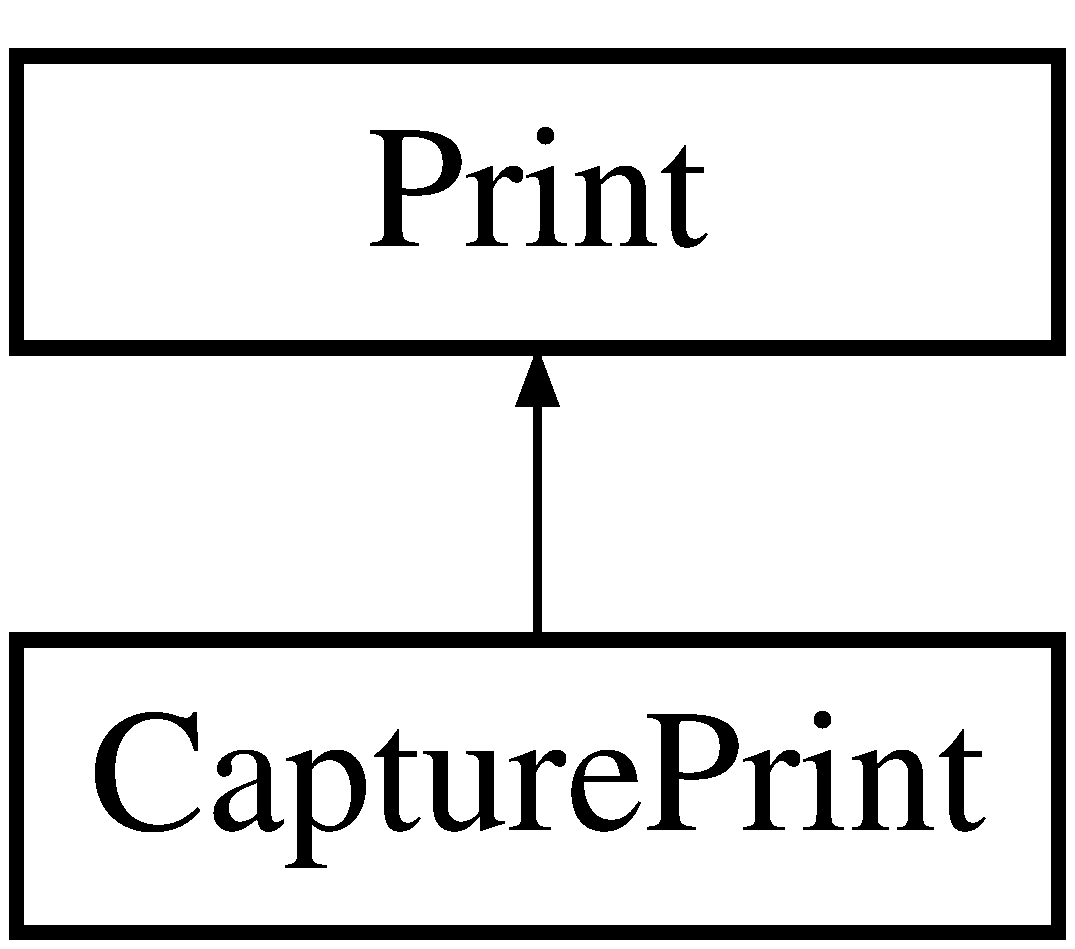
\includegraphics[height=2.000000cm]{class_capture_print}
\end{center}
\end{figure}
\subsection*{Public Member Functions}
\begin{DoxyCompactItemize}
\item 
\hyperlink{class_capture_print_a3b09811c1efd3e7a507627a965a4bdd8}{Capture\+Print} (char $\ast$buffer, int buffer\+Size)
\item 
\hyperlink{class_capture_print_a6e6741b8a50b6ad1c36ebc450798ba18}{Capture\+Print} (char $\ast$buffer, int buffer\+Size, void($\ast$on\+Line\+Finished\+Func)(const \hyperlink{class_capture_print}{Capture\+Print} $\ast$c\+Print), bool($\ast$on\+Buffer\+Overflow\+Func)(const \hyperlink{class_capture_print}{Capture\+Print} $\ast$c\+Print))
\item 
void \hyperlink{class_capture_print_a5ed2798b3b1009eaef1a7927bb50b908}{init} ()
\item 
virtual size\+\_\+t \hyperlink{class_capture_print_aa607f15e4a292e6496af34187732190e}{write} (uint8\+\_\+t c)
\item 
char $\ast$const \& \hyperlink{class_capture_print_a98d6d6a22d52f3a019251a6ca93257c5}{get\+Last\+Line\+Buffer} () const 
\item 
char $\ast$const \& \hyperlink{class_capture_print_a94376bd81d4fab70806fe520a82c2055}{get\+Max\+Buffer\+Size} () const 
\item 
bool \hyperlink{class_capture_print_a87ed8a53df62f7e6367c9885ddf3545d}{overflowed} () const 
\item 
bool \hyperlink{class_capture_print_a3925b40a6e5b62a6206f929ba0f72c7b}{end\+Of\+Line} () const 
\end{DoxyCompactItemize}
\subsection*{Protected Attributes}
\begin{DoxyCompactItemize}
\item 
int \hyperlink{class_capture_print_a2e3ac2d502b2918e3cd58fdd737467b9}{buffer\+Len}
\item 
char $\ast$ \hyperlink{class_capture_print_a25bb02cd05faee2fc28b82c86178c7c6}{data}
\item 
int \hyperlink{class_capture_print_ad7dfa3e9565787e2e80c19fb388c2b05}{data\+Pos}
\item 
bool \hyperlink{class_capture_print_a9f90066b7a79f5cd084e7f7b2ecbe232}{eol}
\item 
bool \hyperlink{class_capture_print_a8ba3d733760230f4c520dc88c81f6911}{current\+Line\+Overflowed}
\item 
void($\ast$ \hyperlink{class_capture_print_a37eb0324e0edeaafb8d4e15118fef58f}{on\+Line\+Finished} )(const \hyperlink{class_capture_print}{Capture\+Print} $\ast$c\+Print)
\item 
bool($\ast$ \hyperlink{class_capture_print_a601a9fdcb038b2e5d818083c58f5fff0}{on\+Buffer\+Overflow} )(const \hyperlink{class_capture_print}{Capture\+Print} $\ast$c\+Print)
\end{DoxyCompactItemize}


\subsection{Detailed Description}
\hyperlink{class_capture_print}{Capture\+Print} implements Print re-\/directing all output to a buffer.
\begin{DoxyItemize}
\item This class will maintain a buffer as a null terminated char\mbox{[}\mbox{]}.
\item This buffer will only ever hold one line, it is flushed on N\+L or C\+R char (~\newline
 smarts inbuilt).
\item \textbackslash{}0 can be printed to this buffer.
\item Full buffers recive no new data until a newline is sent.
\item It can is call a method every newline (~\newline
 smarts inbuilt).
\item It can call a method is called every time an overflow occurs.
\begin{DoxyItemize}
\item If it return true the buffer is reset and overflow flag cleared, allowing for more data.
\end{DoxyItemize}
\end{DoxyItemize}\begin{DoxyWarning}{Warning}
buffer\+Size must be $>$= 2 
\end{DoxyWarning}


\subsection{Constructor \& Destructor Documentation}
\hypertarget{class_capture_print_a3b09811c1efd3e7a507627a965a4bdd8}{}\index{Capture\+Print@{Capture\+Print}!Capture\+Print@{Capture\+Print}}
\index{Capture\+Print@{Capture\+Print}!Capture\+Print@{Capture\+Print}}
\subsubsection[{Capture\+Print(char $\ast$buffer, int buffer\+Size)}]{\setlength{\rightskip}{0pt plus 5cm}Capture\+Print\+::\+Capture\+Print (
\begin{DoxyParamCaption}
\item[{char $\ast$}]{buffer, }
\item[{int}]{buffer\+Size}
\end{DoxyParamCaption}
)\hspace{0.3cm}{\ttfamily [inline]}}\label{class_capture_print_a3b09811c1efd3e7a507627a965a4bdd8}
\hyperlink{class_capture_print}{Capture\+Print} constructor.


\begin{DoxyParams}{Parameters}
{\em buffer} & where data is stored.
\begin{DoxyItemize}
\item This class will maintain the buffer as a null terminated char\mbox{[}\mbox{]}.
\item This buffer will only ever hold one line, it is flushed on N\+L or C\+R char.
\item \textbackslash{}0 can be printed to this buffer.
\item \textbackslash{}0 can be printed to this buffer.
\item Full buffers recive no new data until a newline is sent. 
\end{DoxyItemize}\\
\hline
{\em buffer\+Size} & size of buffer. N\+B\+: buffer\+Size-\/1 is the max string size, to allow for null termination. \\
\hline
\end{DoxyParams}
\begin{DoxyWarning}{Warning}
buffer\+Size must be $>$= 2 
\end{DoxyWarning}
\hypertarget{class_capture_print_a6e6741b8a50b6ad1c36ebc450798ba18}{}\index{Capture\+Print@{Capture\+Print}!Capture\+Print@{Capture\+Print}}
\index{Capture\+Print@{Capture\+Print}!Capture\+Print@{Capture\+Print}}
\subsubsection[{Capture\+Print(char $\ast$buffer, int buffer\+Size, void($\ast$on\+Line\+Finished\+Func)(const Capture\+Print $\ast$c\+Print), bool($\ast$on\+Buffer\+Overflow\+Func)(const Capture\+Print $\ast$c\+Print))}]{\setlength{\rightskip}{0pt plus 5cm}Capture\+Print\+::\+Capture\+Print (
\begin{DoxyParamCaption}
\item[{char $\ast$}]{buffer, }
\item[{int}]{buffer\+Size, }
\item[{void($\ast$)(const {\bf Capture\+Print} $\ast$c\+Print)}]{on\+Line\+Finished\+Func, }
\item[{bool($\ast$)(const {\bf Capture\+Print} $\ast$c\+Print)}]{on\+Buffer\+Overflow\+Func}
\end{DoxyParamCaption}
)}\label{class_capture_print_a6e6741b8a50b6ad1c36ebc450798ba18}
\hyperlink{class_capture_print}{Capture\+Print} constructor.


\begin{DoxyParams}{Parameters}
{\em buffer} & where data is stored.
\begin{DoxyItemize}
\item This class will maintain the buffer as a null terminated char\mbox{[}\mbox{]}.
\item This buffer will only ever hold one line, it is flushed on N\+L or C\+R char (~\newline
 smarts inbuilt).
\item \textbackslash{}0 can be printed to this buffer.
\item Full buffers recive no new data until a newline is sent. 
\end{DoxyItemize}\\
\hline
{\em buffer\+Size} & size of buffer. N\+B\+: buffer\+Size-\/1 is the max string size, to allow for null termination. \\
\hline
{\em on\+Line\+Finished\+Func} & This method is called every newline
\begin{DoxyItemize}
\item ~\newline
 smarts inbuilt.
\item Example function\+: bool on\+Buffer\+Overflow(const Capture\+Print $\ast$c\+Print) \{ \} 
\end{DoxyItemize}\\
\hline
{\em on\+Line\+Finished\+Func} & This method is called every time an overflow occurs.
\begin{DoxyItemize}
\item If it return true the buffer is reset and overflow flag cleared, allowing for more data.
\item Example function\+: void on\+Line\+Finished(const Capture\+Print $\ast$c\+Print) \{ \} 
\end{DoxyItemize}\\
\hline
\end{DoxyParams}
\begin{DoxyWarning}{Warning}
buffer\+Size must be $>$= 2 
\end{DoxyWarning}


\subsection{Member Function Documentation}
\hypertarget{class_capture_print_a3925b40a6e5b62a6206f929ba0f72c7b}{}\index{Capture\+Print@{Capture\+Print}!end\+Of\+Line@{end\+Of\+Line}}
\index{end\+Of\+Line@{end\+Of\+Line}!Capture\+Print@{Capture\+Print}}
\subsubsection[{end\+Of\+Line() const }]{\setlength{\rightskip}{0pt plus 5cm}bool Capture\+Print\+::end\+Of\+Line (
\begin{DoxyParamCaption}
{}
\end{DoxyParamCaption}
) const\hspace{0.3cm}{\ttfamily [inline]}}\label{class_capture_print_a3925b40a6e5b62a6206f929ba0f72c7b}
Return true if we are at the end of the current line (buffer will hold the current line). \hypertarget{class_capture_print_a98d6d6a22d52f3a019251a6ca93257c5}{}\index{Capture\+Print@{Capture\+Print}!get\+Last\+Line\+Buffer@{get\+Last\+Line\+Buffer}}
\index{get\+Last\+Line\+Buffer@{get\+Last\+Line\+Buffer}!Capture\+Print@{Capture\+Print}}
\subsubsection[{get\+Last\+Line\+Buffer() const }]{\setlength{\rightskip}{0pt plus 5cm}char$\ast$ const\& Capture\+Print\+::get\+Last\+Line\+Buffer (
\begin{DoxyParamCaption}
{}
\end{DoxyParamCaption}
) const\hspace{0.3cm}{\ttfamily [inline]}}\label{class_capture_print_a98d6d6a22d52f3a019251a6ca93257c5}
Returns a pointer to the buffer. \hypertarget{class_capture_print_a94376bd81d4fab70806fe520a82c2055}{}\index{Capture\+Print@{Capture\+Print}!get\+Max\+Buffer\+Size@{get\+Max\+Buffer\+Size}}
\index{get\+Max\+Buffer\+Size@{get\+Max\+Buffer\+Size}!Capture\+Print@{Capture\+Print}}
\subsubsection[{get\+Max\+Buffer\+Size() const }]{\setlength{\rightskip}{0pt plus 5cm}char$\ast$ const\& Capture\+Print\+::get\+Max\+Buffer\+Size (
\begin{DoxyParamCaption}
{}
\end{DoxyParamCaption}
) const\hspace{0.3cm}{\ttfamily [inline]}}\label{class_capture_print_a94376bd81d4fab70806fe520a82c2055}
Returns the size of the buffer ({\itshape not} the length of the current string). \hypertarget{class_capture_print_a5ed2798b3b1009eaef1a7927bb50b908}{}\index{Capture\+Print@{Capture\+Print}!init@{init}}
\index{init@{init}!Capture\+Print@{Capture\+Print}}
\subsubsection[{init()}]{\setlength{\rightskip}{0pt plus 5cm}void Capture\+Print\+::init (
\begin{DoxyParamCaption}
{}
\end{DoxyParamCaption}
)}\label{class_capture_print_a5ed2798b3b1009eaef1a7927bb50b908}
Resets the class. N\+B\+: called by constructor, alo suitable for general use. \hypertarget{class_capture_print_a87ed8a53df62f7e6367c9885ddf3545d}{}\index{Capture\+Print@{Capture\+Print}!overflowed@{overflowed}}
\index{overflowed@{overflowed}!Capture\+Print@{Capture\+Print}}
\subsubsection[{overflowed() const }]{\setlength{\rightskip}{0pt plus 5cm}bool Capture\+Print\+::overflowed (
\begin{DoxyParamCaption}
{}
\end{DoxyParamCaption}
) const\hspace{0.3cm}{\ttfamily [inline]}}\label{class_capture_print_a87ed8a53df62f7e6367c9885ddf3545d}
Return true if the buffer overflowed (and overflow was not handled my delegate). \hypertarget{class_capture_print_aa607f15e4a292e6496af34187732190e}{}\index{Capture\+Print@{Capture\+Print}!write@{write}}
\index{write@{write}!Capture\+Print@{Capture\+Print}}
\subsubsection[{write(uint8\+\_\+t c)}]{\setlength{\rightskip}{0pt plus 5cm}size\+\_\+t Capture\+Print\+::write (
\begin{DoxyParamCaption}
\item[{uint8\+\_\+t}]{c}
\end{DoxyParamCaption}
)\hspace{0.3cm}{\ttfamily [virtual]}}\label{class_capture_print_aa607f15e4a292e6496af34187732190e}
Write a character to the buffer. 
\begin{DoxyParams}{Parameters}
{\em c} & character to write. \\
\hline
\end{DoxyParams}


\subsection{Member Data Documentation}
\hypertarget{class_capture_print_a2e3ac2d502b2918e3cd58fdd737467b9}{}\index{Capture\+Print@{Capture\+Print}!buffer\+Len@{buffer\+Len}}
\index{buffer\+Len@{buffer\+Len}!Capture\+Print@{Capture\+Print}}
\subsubsection[{buffer\+Len}]{\setlength{\rightskip}{0pt plus 5cm}int Capture\+Print\+::buffer\+Len\hspace{0.3cm}{\ttfamily [protected]}}\label{class_capture_print_a2e3ac2d502b2918e3cd58fdd737467b9}
\hypertarget{class_capture_print_a8ba3d733760230f4c520dc88c81f6911}{}\index{Capture\+Print@{Capture\+Print}!current\+Line\+Overflowed@{current\+Line\+Overflowed}}
\index{current\+Line\+Overflowed@{current\+Line\+Overflowed}!Capture\+Print@{Capture\+Print}}
\subsubsection[{current\+Line\+Overflowed}]{\setlength{\rightskip}{0pt plus 5cm}bool Capture\+Print\+::current\+Line\+Overflowed\hspace{0.3cm}{\ttfamily [protected]}}\label{class_capture_print_a8ba3d733760230f4c520dc88c81f6911}
\hypertarget{class_capture_print_a25bb02cd05faee2fc28b82c86178c7c6}{}\index{Capture\+Print@{Capture\+Print}!data@{data}}
\index{data@{data}!Capture\+Print@{Capture\+Print}}
\subsubsection[{data}]{\setlength{\rightskip}{0pt plus 5cm}char$\ast$ Capture\+Print\+::data\hspace{0.3cm}{\ttfamily [protected]}}\label{class_capture_print_a25bb02cd05faee2fc28b82c86178c7c6}
\hypertarget{class_capture_print_ad7dfa3e9565787e2e80c19fb388c2b05}{}\index{Capture\+Print@{Capture\+Print}!data\+Pos@{data\+Pos}}
\index{data\+Pos@{data\+Pos}!Capture\+Print@{Capture\+Print}}
\subsubsection[{data\+Pos}]{\setlength{\rightskip}{0pt plus 5cm}int Capture\+Print\+::data\+Pos\hspace{0.3cm}{\ttfamily [protected]}}\label{class_capture_print_ad7dfa3e9565787e2e80c19fb388c2b05}
\hypertarget{class_capture_print_a9f90066b7a79f5cd084e7f7b2ecbe232}{}\index{Capture\+Print@{Capture\+Print}!eol@{eol}}
\index{eol@{eol}!Capture\+Print@{Capture\+Print}}
\subsubsection[{eol}]{\setlength{\rightskip}{0pt plus 5cm}bool Capture\+Print\+::eol\hspace{0.3cm}{\ttfamily [protected]}}\label{class_capture_print_a9f90066b7a79f5cd084e7f7b2ecbe232}
\hypertarget{class_capture_print_a601a9fdcb038b2e5d818083c58f5fff0}{}\index{Capture\+Print@{Capture\+Print}!on\+Buffer\+Overflow@{on\+Buffer\+Overflow}}
\index{on\+Buffer\+Overflow@{on\+Buffer\+Overflow}!Capture\+Print@{Capture\+Print}}
\subsubsection[{on\+Buffer\+Overflow}]{\setlength{\rightskip}{0pt plus 5cm}bool($\ast$ Capture\+Print\+::on\+Buffer\+Overflow) (const {\bf Capture\+Print} $\ast$c\+Print)\hspace{0.3cm}{\ttfamily [protected]}}\label{class_capture_print_a601a9fdcb038b2e5d818083c58f5fff0}
\hypertarget{class_capture_print_a37eb0324e0edeaafb8d4e15118fef58f}{}\index{Capture\+Print@{Capture\+Print}!on\+Line\+Finished@{on\+Line\+Finished}}
\index{on\+Line\+Finished@{on\+Line\+Finished}!Capture\+Print@{Capture\+Print}}
\subsubsection[{on\+Line\+Finished}]{\setlength{\rightskip}{0pt plus 5cm}void($\ast$ Capture\+Print\+::on\+Line\+Finished) (const {\bf Capture\+Print} $\ast$c\+Print)\hspace{0.3cm}{\ttfamily [protected]}}\label{class_capture_print_a37eb0324e0edeaafb8d4e15118fef58f}


The documentation for this class was generated from the following files\+:\begin{DoxyCompactItemize}
\item 
W\+D\+Arduino\+Lib/src/\hyperlink{_capture_print_8h}{Capture\+Print.\+h}\item 
W\+D\+Arduino\+Lib/src/\hyperlink{_capture_print_8cpp}{Capture\+Print.\+cpp}\end{DoxyCompactItemize}

\hypertarget{class_g_n_u_plot_bar_graph}{}\section{G\+N\+U\+Plot\+Bar\+Graph Class Reference}
\label{class_g_n_u_plot_bar_graph}\index{G\+N\+U\+Plot\+Bar\+Graph@{G\+N\+U\+Plot\+Bar\+Graph}}


{\ttfamily \#include $<$G\+N\+U\+Plot.\+h$>$}

Inheritance diagram for G\+N\+U\+Plot\+Bar\+Graph\+:\begin{figure}[H]
\begin{center}
\leavevmode
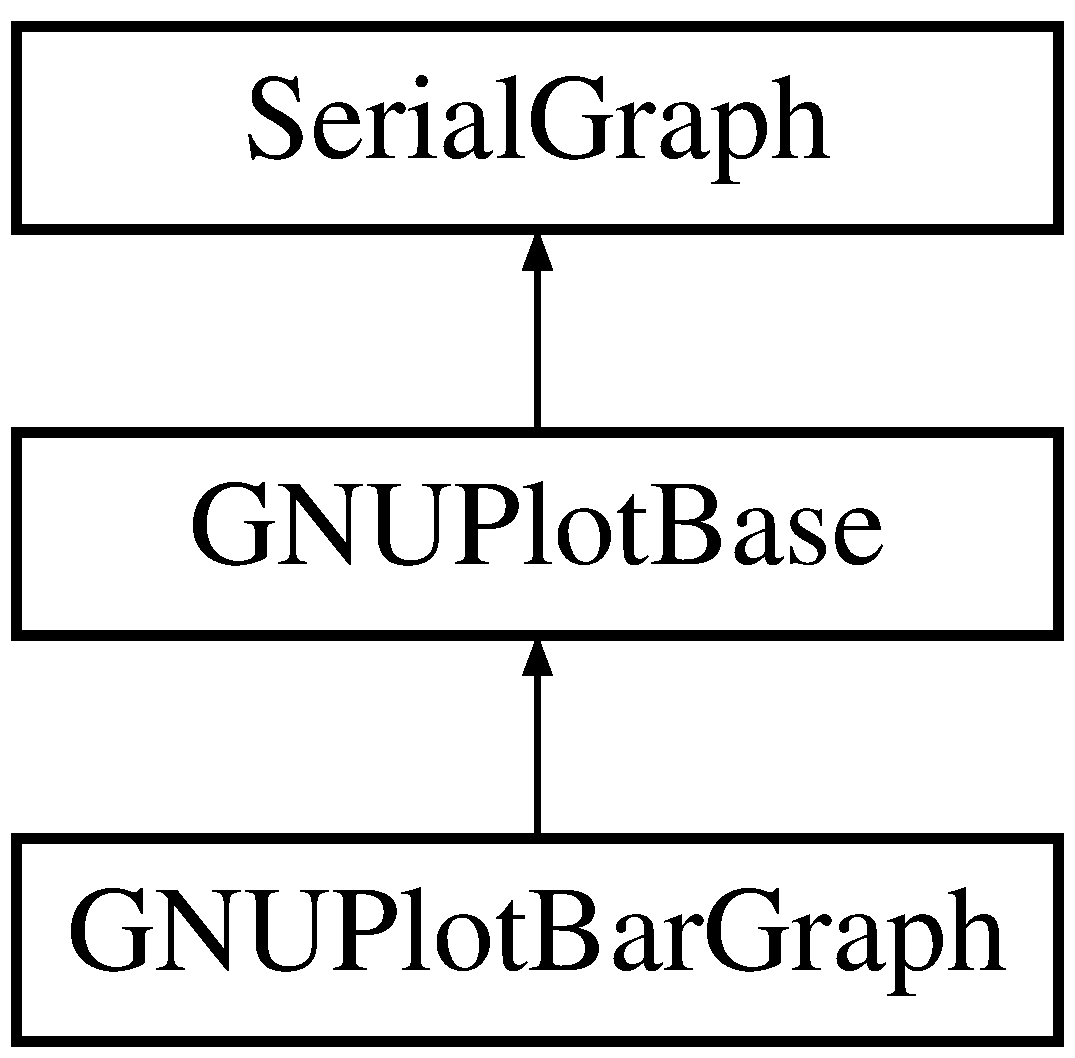
\includegraphics[height=3.000000cm]{class_g_n_u_plot_bar_graph}
\end{center}
\end{figure}
\subsection*{Public Member Functions}
\begin{DoxyCompactItemize}
\item 
\hyperlink{class_g_n_u_plot_bar_graph_ad1e03b9c837e0f6cf9572fcd188ab587}{G\+N\+U\+Plot\+Bar\+Graph} (Print $\ast$\+\_\+out\+Stream)
\item 
virtual \hyperlink{class_g_n_u_plot_bar_graph_a8f589415abcfadb6338a90c2e914be70}{$\sim$\+G\+N\+U\+Plot\+Bar\+Graph} ()
\item 
virtual \hyperlink{_serial_graph_8h_adc73bce6b7e6c4ecf37dde452d6a385e}{Graph\+Style} \hyperlink{class_g_n_u_plot_bar_graph_a6b2cde2832fcb246361d8ebddbe7a228}{get\+Graph\+Style} () const 
\item 
virtual void \hyperlink{class_g_n_u_plot_base_a4d4da234cfdeb99ec3228ef7b2df8a50}{new\+Graph} ()
\item 
virtual void \hyperlink{class_g_n_u_plot_base_aa4b0574c35fbee4dc5f25451eaf956dd}{finish\+Graph} ()
\item 
virtual void \hyperlink{class_g_n_u_plot_base_a219601bd41203477ae73a18d18dd7443}{print\+Comment\+Start} ()
\item 
virtual void \hyperlink{class_serial_graph_a28b020807c52c113685aa6a31f836c52}{enable\+Save\+Image\+File} (bool enabled)
\item 
virtual void \hyperlink{class_serial_graph_abf488e449d6d786bc01478793d0094ad}{set\+Show\+Grid} (bool enabled)
\item 
void \hyperlink{class_serial_graph_a4db09b008589914b71b2ee8b1873db7a}{set\+Title} (const \+\_\+\+\_\+\+Flash\+String\+Helper $\ast$title)
\item 
virtual void \hyperlink{class_serial_graph_ad726b2c84cec50c2d4bfe769e62a9bcd}{set\+Title} (const char $\ast$title)
\item 
void \hyperlink{class_serial_graph_afdb759a860c41de2fc4cfe78519b9fc0}{set\+X\+Axis\+Name} (const \+\_\+\+\_\+\+Flash\+String\+Helper $\ast$title)
\item 
virtual void \hyperlink{class_serial_graph_ac7f30036f5006091af51204a4d9efaf2}{set\+X\+Axis\+Name} (const char $\ast$name)
\item 
void \hyperlink{class_serial_graph_abfc46c15cf8e1b4362a7f51cb11c7bdb}{set\+Y\+Axis\+Name} (const \+\_\+\+\_\+\+Flash\+String\+Helper $\ast$title)
\item 
virtual void \hyperlink{class_serial_graph_ab0c675c8682959261f79dcf37b04148c}{set\+Y\+Axis\+Name} (const char $\ast$name)
\item 
virtual void \hyperlink{class_serial_graph_ae58de4fa4d391f1a2f411ce00dd74d93}{set\+X\+Axis\+Log} (byte scale)
\item 
virtual void \hyperlink{class_serial_graph_a444e38e8ef3784942ca6ee58940f7023}{set\+Y\+Axis\+Log} (byte scale)
\item 
void \hyperlink{class_serial_graph_a84d8e8ce9bff20e53ba738d1d34d3577}{set\+Series\+Name} (int \+\_\+n, const \+\_\+\+\_\+\+Flash\+String\+Helper $\ast$title)
\item 
virtual void \hyperlink{class_serial_graph_a9d67fbecbee6edb82646aa7ba5103046}{set\+Series\+Name} (int \+\_\+n, const char $\ast$name)
\item 
\hyperlink{struct_line_apperance}{Line\+Apperance} $\ast$ \hyperlink{class_serial_graph_a5a6008dc86a2101a58782929721a5b77}{get\+Line\+Apperance} (int \+\_\+n)
\item 
{\footnotesize template$<$typename Y\+T $>$ }\\void \hyperlink{class_serial_graph_afbcc26bd6bad7179d75379ac0f0d25f1}{plot\+Datum\+Y} (Y\+T y1)
\item 
{\footnotesize template$<$typename X\+T , typename Y\+T $>$ }\\void \hyperlink{class_serial_graph_a265b48fb0afe543e14cedb6619e3931e}{plot\+Datum\+X\+Y} (X\+T x, Y\+T y1)
\item 
{\footnotesize template$<$typename Y\+T $>$ }\\void \hyperlink{class_serial_graph_a56f584fa6316175bc9fbcb4f671f1c93}{plot\+Datum\+Yn} (Y\+T y1, Y\+T y2)
\item 
{\footnotesize template$<$typename Y\+T $>$ }\\void \hyperlink{class_serial_graph_ae755b026606e34c33c4aa8f10d8b5d9c}{plot\+Datum\+Yn} (Y\+T y1, Y\+T y2, Y\+T y3)
\item 
{\footnotesize template$<$typename Y\+T $>$ }\\void \hyperlink{class_serial_graph_a354feb95f91239699d3510c2ce5659b0}{plot\+Datum\+Yn} (Y\+T y1, Y\+T y2, Y\+T y3, Y\+T y4)
\item 
{\footnotesize template$<$typename Y\+T $>$ }\\void \hyperlink{class_serial_graph_ab0fff3fc1879e1cd6aadf24c913ff617}{plot\+Datum\+Yn} (Y\+T y1, Y\+T y2, Y\+T y3, Y\+T y4, Y\+T y5)
\item 
{\footnotesize template$<$typename X\+T , typename Y\+T $>$ }\\void \hyperlink{class_serial_graph_aa20b03efac52c18c50efc79c6459a9fc}{plot\+Datum\+Yn} (const Y\+T $\ast$y\+Vec, int \+\_\+n)
\item 
{\footnotesize template$<$typename X\+T , typename Y\+T $>$ }\\void \hyperlink{class_serial_graph_a79b721ca2be68969862869f96d6a6305}{plot\+Datum\+X\+Yn} (X\+T x, Y\+T y1, Y\+T y2)
\item 
{\footnotesize template$<$typename X\+T , typename Y\+T $>$ }\\void \hyperlink{class_serial_graph_a9fcea879f299a7d24be4ff9a38c53c26}{plot\+Datum\+X\+Yn} (X\+T x, Y\+T y1, Y\+T y2, Y\+T y3)
\item 
{\footnotesize template$<$typename X\+T , typename Y\+T $>$ }\\void \hyperlink{class_serial_graph_afd854b631604abe2014a1bb1beeeec52}{plot\+Datum\+X\+Yn} (X\+T x, Y\+T y1, Y\+T y2, Y\+T y3, Y\+T y4)
\item 
{\footnotesize template$<$typename X\+T , typename Y\+T $>$ }\\void \hyperlink{class_serial_graph_aa1bb6fa08a8bd06c074ac2a02b3f6fbc}{plot\+Datum\+X\+Yn} (X\+T x, Y\+T y1, Y\+T y2, Y\+T y3, Y\+T y4, Y\+T y5)
\item 
{\footnotesize template$<$typename X\+T , typename Y\+T $>$ }\\void \hyperlink{class_serial_graph_a3d7276c89235dc1aa176e2439ad9835b}{plot\+Datum\+X\+Yn} (X\+T x, const Y\+T $\ast$y\+Vec, int \+\_\+n)
\item 
{\footnotesize template$<$typename W\+T $>$ }\\void \hyperlink{class_serial_graph_aa72b48968e82a953dcdc6522bd04c7b4}{print} (const W\+T what)
\item 
{\footnotesize template$<$typename W\+T $>$ }\\void \hyperlink{class_serial_graph_a2005d103cb5a578053ef7838b3a8422d}{println} (const W\+T what)
\item 
{\footnotesize template$<$typename W\+T $>$ }\\void \hyperlink{class_serial_graph_a7237d928f67a14d5c9950d8c23c2a794}{print\+Comment} (const W\+T what)
\item 
{\footnotesize template$<$typename W\+T $>$ }\\void \hyperlink{class_serial_graph_a9b40aa22335fc26a6c29b16d278b26f8}{print\+Comment} (const W\+T $\ast$what)
\end{DoxyCompactItemize}
\subsection*{Public Attributes}
\begin{DoxyCompactItemize}
\item 
const byte \hyperlink{class_serial_graph_a1867ab3a93268646490fa7ba4f8b5680}{max\+String\+Size} = 128
\item 
const byte \hyperlink{class_serial_graph_a752a1429bd35687163fe11c5a2562bef}{max\+Series} = 8
\end{DoxyCompactItemize}
\subsection*{Protected Member Functions}
\begin{DoxyCompactItemize}
\item 
virtual void \hyperlink{class_g_n_u_plot_bar_graph_a89a417ec362ccfcaeb23db8438d3579e}{create\+Graph} ()
\item 
{\footnotesize template$<$typename T , typename U $>$ }\\void \hyperlink{class_g_n_u_plot_base_a03d371b0c6c7ef89064525438b22d52c}{set\+Variable} (T name, U value, bool quoted)
\item 
{\footnotesize template$<$typename T $>$ }\\void \hyperlink{class_g_n_u_plot_base_a3c8c8f68c13661d91bd844589e1a2a85}{set\+Variable} (T name)
\item 
{\footnotesize template$<$typename T $>$ }\\void \hyperlink{class_g_n_u_plot_base_af9b418bbcafb41d4d51b92018ca4f217}{unset\+Variable} (T name)
\item 
{\footnotesize template$<$typename T $>$ }\\void \hyperlink{class_g_n_u_plot_base_a68171bf36461e54e2b81384c112ad975}{set\+Varible\+By\+String\+\_\+null\+Safe} (T name, const char $\ast$text)
\item 
{\footnotesize template$<$typename T $>$ }\\void \hyperlink{class_g_n_u_plot_base_ae93c5de3241c2b6b6f703a202dc1d94b}{set\+Varible\+Flag\+By\+Boolean} (T name, bool value)
\item 
void \hyperlink{class_g_n_u_plot_base_ab5c851953dd140cc3ee936a5cd329200}{save\+Plot\+To\+Image\+File} (const char $\ast$title)
\item 
virtual void \hyperlink{class_g_n_u_plot_base_adaf91c191e4d889537d401faeb863485}{make\+Ready\+For\+Plot\+Data} ()
\item 
char $\ast$ \hyperlink{class_g_n_u_plot_base_a7f71f3c616b3a4a854f9118a04c40447}{malloc\+Basic\+File\+Name\+From\+Graph\+Title} ()
\item 
void \hyperlink{class_g_n_u_plot_base_a65ae2b3220034bce21c7feb39a632991}{print\+Title\+In\+Plot\+Command} (int series\+Num)
\item 
void \hyperlink{class_g_n_u_plot_base_ad057969aa7f8bdbe884d6a5d03a29722}{print\+Line\+Apperance} (\hyperlink{struct_line_apperance}{Line\+Apperance} apperance)
\item 
void \hyperlink{class_g_n_u_plot_base_ad7e8ef8d8e5eb80119fc0cce9be2d525}{print\+Log\+Axis\+Command} (const \+\_\+\+\_\+\+Flash\+String\+Helper $\ast$axis\+Name, byte log\+Scale)
\item 
virtual void \hyperlink{class_g_n_u_plot_base_ae204818b4e8dcd9d2f6b5426127ca2cf}{print\+Seperator} ()
\item 
virtual void \hyperlink{class_g_n_u_plot_base_ac2b48b822b6043392b514c9580b1661a}{print\+Start\+Datum} ()
\item 
virtual void \hyperlink{class_g_n_u_plot_base_aff02bc279e6c3cb83f2cdc7aa021268f}{print\+End\+Datum} ()
\item 
virtual void \hyperlink{class_g_n_u_plot_base_ad00a12fd681e4638fae005891fd72f38}{\+\_\+print\+Data\+Value} (const char $\ast$value)
\item 
virtual void \hyperlink{class_g_n_u_plot_base_aa6c6dfff0568dd99c0c28081c41b4433}{\+\_\+print\+Data\+Value} (char value)
\item 
virtual void \hyperlink{class_g_n_u_plot_base_a6f14fc040ff833c685ab09fc7917e059}{\+\_\+print\+Data\+Value} (bool value)
\item 
virtual void \hyperlink{class_serial_graph_a0c4d2c1239de3107d7332389183b05a1}{\+\_\+print\+Data\+Value} (const \+\_\+\+\_\+\+Flash\+String\+Helper $\ast$value)
\item 
virtual void \hyperlink{class_serial_graph_a58edf4683c600b6bfa1714b0f8dfc82c}{\+\_\+print\+Data\+Value} (int value)
\item 
virtual void \hyperlink{class_serial_graph_a9a4903d4fa26bb85ba5dd93c4365bcc2}{\+\_\+print\+Data\+Value} (long value)
\item 
virtual void \hyperlink{class_serial_graph_acada5333b96b65e31d8c76c3ab22905f}{\+\_\+print\+Data\+Value} (byte value)
\item 
virtual void \hyperlink{class_serial_graph_acd91cf0c3a0f49d4bdf18b447503da23}{\+\_\+print\+Data\+Value} (unsigned int value)
\item 
virtual void \hyperlink{class_serial_graph_a6dbfe61ee398e18c1b752a3748df9663}{\+\_\+print\+Data\+Value} (unsigned long value)
\item 
virtual void \hyperlink{class_serial_graph_a766d5838ede9c8fa998ce8664e5f92be}{\+\_\+print\+Data\+Value} (double value)
\item 
void \hyperlink{class_serial_graph_a760dd00474c9780c81ece7cdf621fc15}{init} ()
\item 
void \hyperlink{class_serial_graph_abd43150abedec26eef3994cd33035173}{ensure\+Ready\+To\+Recive\+Plot\+Data} ()
\item 
{\footnotesize template$<$typename T $>$ }\\void \hyperlink{class_serial_graph_a91e20c05c8cc612fd9ffd85880149264}{print\+Data\+Value} (T value)
\end{DoxyCompactItemize}
\subsection*{Protected Attributes}
\begin{DoxyCompactItemize}
\item 
bool \hyperlink{class_serial_graph_a24202e0a7a8bac5ec1cfd92bf796e078}{save\+File}
\item 
Print $\ast$ \hyperlink{class_serial_graph_aec32289a9393e98bf80d44406e5c207d}{out\+Stream}
\item 
bool \hyperlink{class_serial_graph_a4dbd9cf190c591fb4f2f46a50d937199}{x\+Axis\+Specified}
\item 
int \hyperlink{class_serial_graph_ab40c430e06102b9624736173d4a58596}{num\+Y\+Series}
\item 
bool \hyperlink{class_serial_graph_ad61d5ea29eacc1611c5addc94714f1e2}{show\+Grid}
\item 
char $\ast$ \hyperlink{class_serial_graph_a0b33d43c2bb54340ef1f90b5f76d7aea}{graph\+Title}
\item 
char $\ast$ \hyperlink{class_serial_graph_a5f5bf85ed361ff567d0888eaa73e269c}{x\+Axis\+Name}
\item 
char $\ast$ \hyperlink{class_serial_graph_a08452a56c74ec5f5473b64605d555339}{y\+Axis\+Name}
\item 
char $\ast$$\ast$ \hyperlink{class_serial_graph_a2307e40e27249f44bbe14776dc68c561}{series\+Names}
\item 
\hyperlink{struct_line_apperance}{Line\+Apperance} $\ast$ \hyperlink{class_serial_graph_a8d743f9eeeca69a988d2159a405e4253}{series\+Apperance}
\item 
byte \hyperlink{class_serial_graph_afc2ca72fdfe2bc5e3159c9e910a8f81e}{x\+Axis\+Log\+Scale}
\item 
byte \hyperlink{class_serial_graph_a1f0424857ec14c176747b3ddb0768eee}{y\+Axis\+Log\+Scale}
\end{DoxyCompactItemize}


\subsection{Detailed Description}
Specilisation of \hyperlink{class_g_n_u_plot_base}{G\+N\+U\+Plot\+Base} to make bar graphs. 

\subsection{Constructor \& Destructor Documentation}
\hypertarget{class_g_n_u_plot_bar_graph_ad1e03b9c837e0f6cf9572fcd188ab587}{}\index{G\+N\+U\+Plot\+Bar\+Graph@{G\+N\+U\+Plot\+Bar\+Graph}!G\+N\+U\+Plot\+Bar\+Graph@{G\+N\+U\+Plot\+Bar\+Graph}}
\index{G\+N\+U\+Plot\+Bar\+Graph@{G\+N\+U\+Plot\+Bar\+Graph}!G\+N\+U\+Plot\+Bar\+Graph@{G\+N\+U\+Plot\+Bar\+Graph}}
\subsubsection[{G\+N\+U\+Plot\+Bar\+Graph(\+Print $\ast$\+\_\+out\+Stream)}]{\setlength{\rightskip}{0pt plus 5cm}G\+N\+U\+Plot\+Bar\+Graph\+::\+G\+N\+U\+Plot\+Bar\+Graph (
\begin{DoxyParamCaption}
\item[{Print $\ast$}]{\+\_\+out\+Stream}
\end{DoxyParamCaption}
)\hspace{0.3cm}{\ttfamily [inline]}}\label{class_g_n_u_plot_bar_graph_ad1e03b9c837e0f6cf9572fcd188ab587}
\hypertarget{class_g_n_u_plot_bar_graph_a8f589415abcfadb6338a90c2e914be70}{}\index{G\+N\+U\+Plot\+Bar\+Graph@{G\+N\+U\+Plot\+Bar\+Graph}!````~G\+N\+U\+Plot\+Bar\+Graph@{$\sim$\+G\+N\+U\+Plot\+Bar\+Graph}}
\index{````~G\+N\+U\+Plot\+Bar\+Graph@{$\sim$\+G\+N\+U\+Plot\+Bar\+Graph}!G\+N\+U\+Plot\+Bar\+Graph@{G\+N\+U\+Plot\+Bar\+Graph}}
\subsubsection[{$\sim$\+G\+N\+U\+Plot\+Bar\+Graph()}]{\setlength{\rightskip}{0pt plus 5cm}virtual G\+N\+U\+Plot\+Bar\+Graph\+::$\sim$\+G\+N\+U\+Plot\+Bar\+Graph (
\begin{DoxyParamCaption}
{}
\end{DoxyParamCaption}
)\hspace{0.3cm}{\ttfamily [inline]}, {\ttfamily [virtual]}}\label{class_g_n_u_plot_bar_graph_a8f589415abcfadb6338a90c2e914be70}


\subsection{Member Function Documentation}
\hypertarget{class_g_n_u_plot_base_ad00a12fd681e4638fae005891fd72f38}{}\index{G\+N\+U\+Plot\+Bar\+Graph@{G\+N\+U\+Plot\+Bar\+Graph}!\+\_\+print\+Data\+Value@{\+\_\+print\+Data\+Value}}
\index{\+\_\+print\+Data\+Value@{\+\_\+print\+Data\+Value}!G\+N\+U\+Plot\+Bar\+Graph@{G\+N\+U\+Plot\+Bar\+Graph}}
\subsubsection[{\+\_\+print\+Data\+Value(const char $\ast$value)}]{\setlength{\rightskip}{0pt plus 5cm}void G\+N\+U\+Plot\+Base\+::\+\_\+print\+Data\+Value (
\begin{DoxyParamCaption}
\item[{const char $\ast$}]{value}
\end{DoxyParamCaption}
)\hspace{0.3cm}{\ttfamily [protected]}, {\ttfamily [virtual]}, {\ttfamily [inherited]}}\label{class_g_n_u_plot_base_ad00a12fd681e4638fae005891fd72f38}
Override a put appropriate quotes around strings etc. 
\begin{DoxyParams}{Parameters}
{\em value} & What to print. \\
\hline
\end{DoxyParams}


Reimplemented from \hyperlink{class_serial_graph_a8252997dd4bad0251d437d6dd097bffb}{Serial\+Graph}.

\hypertarget{class_g_n_u_plot_base_aa6c6dfff0568dd99c0c28081c41b4433}{}\index{G\+N\+U\+Plot\+Bar\+Graph@{G\+N\+U\+Plot\+Bar\+Graph}!\+\_\+print\+Data\+Value@{\+\_\+print\+Data\+Value}}
\index{\+\_\+print\+Data\+Value@{\+\_\+print\+Data\+Value}!G\+N\+U\+Plot\+Bar\+Graph@{G\+N\+U\+Plot\+Bar\+Graph}}
\subsubsection[{\+\_\+print\+Data\+Value(char value)}]{\setlength{\rightskip}{0pt plus 5cm}virtual void G\+N\+U\+Plot\+Base\+::\+\_\+print\+Data\+Value (
\begin{DoxyParamCaption}
\item[{char}]{value}
\end{DoxyParamCaption}
)\hspace{0.3cm}{\ttfamily [inline]}, {\ttfamily [protected]}, {\ttfamily [virtual]}, {\ttfamily [inherited]}}\label{class_g_n_u_plot_base_aa6c6dfff0568dd99c0c28081c41b4433}
Override for customised value output. 
\begin{DoxyParams}{Parameters}
{\em value} & What to print. \\
\hline
\end{DoxyParams}


Reimplemented from \hyperlink{class_serial_graph_af3fbf7a9201f71cd6bad7e4337092fb6}{Serial\+Graph}.

\hypertarget{class_g_n_u_plot_base_a6f14fc040ff833c685ab09fc7917e059}{}\index{G\+N\+U\+Plot\+Bar\+Graph@{G\+N\+U\+Plot\+Bar\+Graph}!\+\_\+print\+Data\+Value@{\+\_\+print\+Data\+Value}}
\index{\+\_\+print\+Data\+Value@{\+\_\+print\+Data\+Value}!G\+N\+U\+Plot\+Bar\+Graph@{G\+N\+U\+Plot\+Bar\+Graph}}
\subsubsection[{\+\_\+print\+Data\+Value(bool value)}]{\setlength{\rightskip}{0pt plus 5cm}virtual void G\+N\+U\+Plot\+Base\+::\+\_\+print\+Data\+Value (
\begin{DoxyParamCaption}
\item[{bool}]{value}
\end{DoxyParamCaption}
)\hspace{0.3cm}{\ttfamily [inline]}, {\ttfamily [protected]}, {\ttfamily [virtual]}, {\ttfamily [inherited]}}\label{class_g_n_u_plot_base_a6f14fc040ff833c685ab09fc7917e059}
Override for customised value output. 
\begin{DoxyParams}{Parameters}
{\em value} & What to print. \\
\hline
\end{DoxyParams}


Reimplemented from \hyperlink{class_serial_graph_aed9ff95634ace3d190863ea9d15c10da}{Serial\+Graph}.

\hypertarget{class_serial_graph_a0c4d2c1239de3107d7332389183b05a1}{}\index{G\+N\+U\+Plot\+Bar\+Graph@{G\+N\+U\+Plot\+Bar\+Graph}!\+\_\+print\+Data\+Value@{\+\_\+print\+Data\+Value}}
\index{\+\_\+print\+Data\+Value@{\+\_\+print\+Data\+Value}!G\+N\+U\+Plot\+Bar\+Graph@{G\+N\+U\+Plot\+Bar\+Graph}}
\subsubsection[{\+\_\+print\+Data\+Value(const \+\_\+\+\_\+\+Flash\+String\+Helper $\ast$value)}]{\setlength{\rightskip}{0pt plus 5cm}virtual void Serial\+Graph\+::\+\_\+print\+Data\+Value (
\begin{DoxyParamCaption}
\item[{const \+\_\+\+\_\+\+Flash\+String\+Helper $\ast$}]{value}
\end{DoxyParamCaption}
)\hspace{0.3cm}{\ttfamily [inline]}, {\ttfamily [protected]}, {\ttfamily [virtual]}, {\ttfamily [inherited]}}\label{class_serial_graph_a0c4d2c1239de3107d7332389183b05a1}
This just calls \hyperlink{class_serial_graph_a8252997dd4bad0251d437d6dd097bffb}{\+\_\+print\+Data\+Value(const char $\ast$value)} so probably alter that instead. 
\begin{DoxyParams}{Parameters}
{\em value} & What to print. \\
\hline
\end{DoxyParams}
\hypertarget{class_serial_graph_a58edf4683c600b6bfa1714b0f8dfc82c}{}\index{G\+N\+U\+Plot\+Bar\+Graph@{G\+N\+U\+Plot\+Bar\+Graph}!\+\_\+print\+Data\+Value@{\+\_\+print\+Data\+Value}}
\index{\+\_\+print\+Data\+Value@{\+\_\+print\+Data\+Value}!G\+N\+U\+Plot\+Bar\+Graph@{G\+N\+U\+Plot\+Bar\+Graph}}
\subsubsection[{\+\_\+print\+Data\+Value(int value)}]{\setlength{\rightskip}{0pt plus 5cm}virtual void Serial\+Graph\+::\+\_\+print\+Data\+Value (
\begin{DoxyParamCaption}
\item[{int}]{value}
\end{DoxyParamCaption}
)\hspace{0.3cm}{\ttfamily [inline]}, {\ttfamily [protected]}, {\ttfamily [virtual]}, {\ttfamily [inherited]}}\label{class_serial_graph_a58edf4683c600b6bfa1714b0f8dfc82c}
Override for customised value output. 
\begin{DoxyParams}{Parameters}
{\em value} & What to print. \\
\hline
\end{DoxyParams}
\hypertarget{class_serial_graph_a9a4903d4fa26bb85ba5dd93c4365bcc2}{}\index{G\+N\+U\+Plot\+Bar\+Graph@{G\+N\+U\+Plot\+Bar\+Graph}!\+\_\+print\+Data\+Value@{\+\_\+print\+Data\+Value}}
\index{\+\_\+print\+Data\+Value@{\+\_\+print\+Data\+Value}!G\+N\+U\+Plot\+Bar\+Graph@{G\+N\+U\+Plot\+Bar\+Graph}}
\subsubsection[{\+\_\+print\+Data\+Value(long value)}]{\setlength{\rightskip}{0pt plus 5cm}virtual void Serial\+Graph\+::\+\_\+print\+Data\+Value (
\begin{DoxyParamCaption}
\item[{long}]{value}
\end{DoxyParamCaption}
)\hspace{0.3cm}{\ttfamily [inline]}, {\ttfamily [protected]}, {\ttfamily [virtual]}, {\ttfamily [inherited]}}\label{class_serial_graph_a9a4903d4fa26bb85ba5dd93c4365bcc2}
Override for customised value output. 
\begin{DoxyParams}{Parameters}
{\em value} & What to print. \\
\hline
\end{DoxyParams}
\hypertarget{class_serial_graph_acada5333b96b65e31d8c76c3ab22905f}{}\index{G\+N\+U\+Plot\+Bar\+Graph@{G\+N\+U\+Plot\+Bar\+Graph}!\+\_\+print\+Data\+Value@{\+\_\+print\+Data\+Value}}
\index{\+\_\+print\+Data\+Value@{\+\_\+print\+Data\+Value}!G\+N\+U\+Plot\+Bar\+Graph@{G\+N\+U\+Plot\+Bar\+Graph}}
\subsubsection[{\+\_\+print\+Data\+Value(byte value)}]{\setlength{\rightskip}{0pt plus 5cm}virtual void Serial\+Graph\+::\+\_\+print\+Data\+Value (
\begin{DoxyParamCaption}
\item[{byte}]{value}
\end{DoxyParamCaption}
)\hspace{0.3cm}{\ttfamily [inline]}, {\ttfamily [protected]}, {\ttfamily [virtual]}, {\ttfamily [inherited]}}\label{class_serial_graph_acada5333b96b65e31d8c76c3ab22905f}
Override for customised value output. 
\begin{DoxyParams}{Parameters}
{\em value} & What to print. \\
\hline
\end{DoxyParams}
\hypertarget{class_serial_graph_acd91cf0c3a0f49d4bdf18b447503da23}{}\index{G\+N\+U\+Plot\+Bar\+Graph@{G\+N\+U\+Plot\+Bar\+Graph}!\+\_\+print\+Data\+Value@{\+\_\+print\+Data\+Value}}
\index{\+\_\+print\+Data\+Value@{\+\_\+print\+Data\+Value}!G\+N\+U\+Plot\+Bar\+Graph@{G\+N\+U\+Plot\+Bar\+Graph}}
\subsubsection[{\+\_\+print\+Data\+Value(unsigned int value)}]{\setlength{\rightskip}{0pt plus 5cm}virtual void Serial\+Graph\+::\+\_\+print\+Data\+Value (
\begin{DoxyParamCaption}
\item[{unsigned int}]{value}
\end{DoxyParamCaption}
)\hspace{0.3cm}{\ttfamily [inline]}, {\ttfamily [protected]}, {\ttfamily [virtual]}, {\ttfamily [inherited]}}\label{class_serial_graph_acd91cf0c3a0f49d4bdf18b447503da23}
Override for customised value output. 
\begin{DoxyParams}{Parameters}
{\em value} & What to print. \\
\hline
\end{DoxyParams}
\hypertarget{class_serial_graph_a6dbfe61ee398e18c1b752a3748df9663}{}\index{G\+N\+U\+Plot\+Bar\+Graph@{G\+N\+U\+Plot\+Bar\+Graph}!\+\_\+print\+Data\+Value@{\+\_\+print\+Data\+Value}}
\index{\+\_\+print\+Data\+Value@{\+\_\+print\+Data\+Value}!G\+N\+U\+Plot\+Bar\+Graph@{G\+N\+U\+Plot\+Bar\+Graph}}
\subsubsection[{\+\_\+print\+Data\+Value(unsigned long value)}]{\setlength{\rightskip}{0pt plus 5cm}virtual void Serial\+Graph\+::\+\_\+print\+Data\+Value (
\begin{DoxyParamCaption}
\item[{unsigned long}]{value}
\end{DoxyParamCaption}
)\hspace{0.3cm}{\ttfamily [inline]}, {\ttfamily [protected]}, {\ttfamily [virtual]}, {\ttfamily [inherited]}}\label{class_serial_graph_a6dbfe61ee398e18c1b752a3748df9663}
Override for customised value output. 
\begin{DoxyParams}{Parameters}
{\em value} & What to print. \\
\hline
\end{DoxyParams}
\hypertarget{class_serial_graph_a766d5838ede9c8fa998ce8664e5f92be}{}\index{G\+N\+U\+Plot\+Bar\+Graph@{G\+N\+U\+Plot\+Bar\+Graph}!\+\_\+print\+Data\+Value@{\+\_\+print\+Data\+Value}}
\index{\+\_\+print\+Data\+Value@{\+\_\+print\+Data\+Value}!G\+N\+U\+Plot\+Bar\+Graph@{G\+N\+U\+Plot\+Bar\+Graph}}
\subsubsection[{\+\_\+print\+Data\+Value(double value)}]{\setlength{\rightskip}{0pt plus 5cm}virtual void Serial\+Graph\+::\+\_\+print\+Data\+Value (
\begin{DoxyParamCaption}
\item[{double}]{value}
\end{DoxyParamCaption}
)\hspace{0.3cm}{\ttfamily [inline]}, {\ttfamily [protected]}, {\ttfamily [virtual]}, {\ttfamily [inherited]}}\label{class_serial_graph_a766d5838ede9c8fa998ce8664e5f92be}
Override for customised value output. 
\begin{DoxyParams}{Parameters}
{\em value} & What to print. \\
\hline
\end{DoxyParams}
\hypertarget{class_g_n_u_plot_bar_graph_a89a417ec362ccfcaeb23db8438d3579e}{}\index{G\+N\+U\+Plot\+Bar\+Graph@{G\+N\+U\+Plot\+Bar\+Graph}!create\+Graph@{create\+Graph}}
\index{create\+Graph@{create\+Graph}!G\+N\+U\+Plot\+Bar\+Graph@{G\+N\+U\+Plot\+Bar\+Graph}}
\subsubsection[{create\+Graph()}]{\setlength{\rightskip}{0pt plus 5cm}void G\+N\+U\+Plot\+Bar\+Graph\+::create\+Graph (
\begin{DoxyParamCaption}
{}
\end{DoxyParamCaption}
)\hspace{0.3cm}{\ttfamily [protected]}, {\ttfamily [virtual]}}\label{class_g_n_u_plot_bar_graph_a89a417ec362ccfcaeb23db8438d3579e}


Implements \hyperlink{class_g_n_u_plot_base_ad877f207d43e6f9cd0aa0ef241e31c24}{G\+N\+U\+Plot\+Base}.

\hypertarget{class_serial_graph_a28b020807c52c113685aa6a31f836c52}{}\index{G\+N\+U\+Plot\+Bar\+Graph@{G\+N\+U\+Plot\+Bar\+Graph}!enable\+Save\+Image\+File@{enable\+Save\+Image\+File}}
\index{enable\+Save\+Image\+File@{enable\+Save\+Image\+File}!G\+N\+U\+Plot\+Bar\+Graph@{G\+N\+U\+Plot\+Bar\+Graph}}
\subsubsection[{enable\+Save\+Image\+File(bool enabled)}]{\setlength{\rightskip}{0pt plus 5cm}virtual void Serial\+Graph\+::enable\+Save\+Image\+File (
\begin{DoxyParamCaption}
\item[{bool}]{enabled}
\end{DoxyParamCaption}
)\hspace{0.3cm}{\ttfamily [inline]}, {\ttfamily [virtual]}, {\ttfamily [inherited]}}\label{class_serial_graph_a28b020807c52c113685aa6a31f836c52}
Set to true if an image file should be saved. \begin{DoxyNote}{Note}
Filename will be based on graph title. This is done to save memory. Final filename has some extra validation performed to conform with filename rules aplicable to modern operating systems (excluding 8 char limit). 
\end{DoxyNote}
\hypertarget{class_serial_graph_abd43150abedec26eef3994cd33035173}{}\index{G\+N\+U\+Plot\+Bar\+Graph@{G\+N\+U\+Plot\+Bar\+Graph}!ensure\+Ready\+To\+Recive\+Plot\+Data@{ensure\+Ready\+To\+Recive\+Plot\+Data}}
\index{ensure\+Ready\+To\+Recive\+Plot\+Data@{ensure\+Ready\+To\+Recive\+Plot\+Data}!G\+N\+U\+Plot\+Bar\+Graph@{G\+N\+U\+Plot\+Bar\+Graph}}
\subsubsection[{ensure\+Ready\+To\+Recive\+Plot\+Data()}]{\setlength{\rightskip}{0pt plus 5cm}void Serial\+Graph\+::ensure\+Ready\+To\+Recive\+Plot\+Data (
\begin{DoxyParamCaption}
{}
\end{DoxyParamCaption}
)\hspace{0.3cm}{\ttfamily [protected]}, {\ttfamily [inherited]}}\label{class_serial_graph_abd43150abedec26eef3994cd33035173}
Called by every plot command prior to sending data. it\textquotesingle{}s function is to call \hyperlink{class_serial_graph_a898cf274c886e0ff45e90d3f21f0a6cc}{make\+Ready\+For\+Plot\+Data()} the first time it is called. 
\begin{DoxyParams}{Parameters}
{\em value} & What to print. \\
\hline
\end{DoxyParams}
\hypertarget{class_g_n_u_plot_base_aa4b0574c35fbee4dc5f25451eaf956dd}{}\index{G\+N\+U\+Plot\+Bar\+Graph@{G\+N\+U\+Plot\+Bar\+Graph}!finish\+Graph@{finish\+Graph}}
\index{finish\+Graph@{finish\+Graph}!G\+N\+U\+Plot\+Bar\+Graph@{G\+N\+U\+Plot\+Bar\+Graph}}
\subsubsection[{finish\+Graph()}]{\setlength{\rightskip}{0pt plus 5cm}void G\+N\+U\+Plot\+Base\+::finish\+Graph (
\begin{DoxyParamCaption}
{}
\end{DoxyParamCaption}
)\hspace{0.3cm}{\ttfamily [virtual]}, {\ttfamily [inherited]}}\label{class_g_n_u_plot_base_aa4b0574c35fbee4dc5f25451eaf956dd}
Serial output that finishes the plot, saves file, updates display etc. 

Implements \hyperlink{class_serial_graph_a8054ce989a1788bd35d2fde56081c88c}{Serial\+Graph}.

\hypertarget{class_g_n_u_plot_bar_graph_a6b2cde2832fcb246361d8ebddbe7a228}{}\index{G\+N\+U\+Plot\+Bar\+Graph@{G\+N\+U\+Plot\+Bar\+Graph}!get\+Graph\+Style@{get\+Graph\+Style}}
\index{get\+Graph\+Style@{get\+Graph\+Style}!G\+N\+U\+Plot\+Bar\+Graph@{G\+N\+U\+Plot\+Bar\+Graph}}
\subsubsection[{get\+Graph\+Style() const }]{\setlength{\rightskip}{0pt plus 5cm}virtual {\bf Graph\+Style} G\+N\+U\+Plot\+Bar\+Graph\+::get\+Graph\+Style (
\begin{DoxyParamCaption}
{}
\end{DoxyParamCaption}
) const\hspace{0.3cm}{\ttfamily [inline]}, {\ttfamily [virtual]}}\label{class_g_n_u_plot_bar_graph_a6b2cde2832fcb246361d8ebddbe7a228}
Returns the Graph\+Style of the current object. 

Implements \hyperlink{class_serial_graph_a2ab97096fffdf429bfa271b9fd4c642a}{Serial\+Graph}.

\hypertarget{class_serial_graph_a5a6008dc86a2101a58782929721a5b77}{}\index{G\+N\+U\+Plot\+Bar\+Graph@{G\+N\+U\+Plot\+Bar\+Graph}!get\+Line\+Apperance@{get\+Line\+Apperance}}
\index{get\+Line\+Apperance@{get\+Line\+Apperance}!G\+N\+U\+Plot\+Bar\+Graph@{G\+N\+U\+Plot\+Bar\+Graph}}
\subsubsection[{get\+Line\+Apperance(int \+\_\+n)}]{\setlength{\rightskip}{0pt plus 5cm}{\bf Line\+Apperance}$\ast$ Serial\+Graph\+::get\+Line\+Apperance (
\begin{DoxyParamCaption}
\item[{int}]{\+\_\+n}
\end{DoxyParamCaption}
)\hspace{0.3cm}{\ttfamily [inline]}, {\ttfamily [inherited]}}\label{class_serial_graph_a5a6008dc86a2101a58782929721a5b77}
Gets a structure that controls apperance of a series (called a \hyperlink{struct_line_apperance}{Line\+Apperance}). It is intended that you directly modify the structure returned, there is no set\+Line\+Apperance. See the struct \hyperlink{struct_line_apperance}{Line\+Apperance} for more.


\begin{DoxyParams}{Parameters}
{\em \+\_\+n} & Series number to alter.\\
\hline
\end{DoxyParams}
\begin{DoxyNote}{Note}
Behaviour on \+\_\+n $>$ max\+Series, is to just override the last possible series entry. 
\end{DoxyNote}
\hypertarget{class_serial_graph_a760dd00474c9780c81ece7cdf621fc15}{}\index{G\+N\+U\+Plot\+Bar\+Graph@{G\+N\+U\+Plot\+Bar\+Graph}!init@{init}}
\index{init@{init}!G\+N\+U\+Plot\+Bar\+Graph@{G\+N\+U\+Plot\+Bar\+Graph}}
\subsubsection[{init()}]{\setlength{\rightskip}{0pt plus 5cm}void Serial\+Graph\+::init (
\begin{DoxyParamCaption}
{}
\end{DoxyParamCaption}
)\hspace{0.3cm}{\ttfamily [protected]}, {\ttfamily [inherited]}}\label{class_serial_graph_a760dd00474c9780c81ece7cdf621fc15}
Brings the class to its default state. Called by the constructor and \hyperlink{class_serial_graph_a44d34593c56aa67142ccd9fcc0a1da86}{new\+Graph()}. \hypertarget{class_g_n_u_plot_base_adaf91c191e4d889537d401faeb863485}{}\index{G\+N\+U\+Plot\+Bar\+Graph@{G\+N\+U\+Plot\+Bar\+Graph}!make\+Ready\+For\+Plot\+Data@{make\+Ready\+For\+Plot\+Data}}
\index{make\+Ready\+For\+Plot\+Data@{make\+Ready\+For\+Plot\+Data}!G\+N\+U\+Plot\+Bar\+Graph@{G\+N\+U\+Plot\+Bar\+Graph}}
\subsubsection[{make\+Ready\+For\+Plot\+Data()}]{\setlength{\rightskip}{0pt plus 5cm}void G\+N\+U\+Plot\+Base\+::make\+Ready\+For\+Plot\+Data (
\begin{DoxyParamCaption}
{}
\end{DoxyParamCaption}
)\hspace{0.3cm}{\ttfamily [protected]}, {\ttfamily [virtual]}, {\ttfamily [inherited]}}\label{class_g_n_u_plot_base_adaf91c191e4d889537d401faeb863485}
Called by ensure\+Ready\+To\+Recive\+Plot\+Data, if the first plot command is encountered. \begin{DoxyNote}{Note}
A concrete class should override this. 
\end{DoxyNote}


Reimplemented from \hyperlink{class_serial_graph_a898cf274c886e0ff45e90d3f21f0a6cc}{Serial\+Graph}.

\hypertarget{class_g_n_u_plot_base_a7f71f3c616b3a4a854f9118a04c40447}{}\index{G\+N\+U\+Plot\+Bar\+Graph@{G\+N\+U\+Plot\+Bar\+Graph}!malloc\+Basic\+File\+Name\+From\+Graph\+Title@{malloc\+Basic\+File\+Name\+From\+Graph\+Title}}
\index{malloc\+Basic\+File\+Name\+From\+Graph\+Title@{malloc\+Basic\+File\+Name\+From\+Graph\+Title}!G\+N\+U\+Plot\+Bar\+Graph@{G\+N\+U\+Plot\+Bar\+Graph}}
\subsubsection[{malloc\+Basic\+File\+Name\+From\+Graph\+Title()}]{\setlength{\rightskip}{0pt plus 5cm}char $\ast$ G\+N\+U\+Plot\+Base\+::malloc\+Basic\+File\+Name\+From\+Graph\+Title (
\begin{DoxyParamCaption}
{}
\end{DoxyParamCaption}
)\hspace{0.3cm}{\ttfamily [protected]}, {\ttfamily [inherited]}}\label{class_g_n_u_plot_base_a7f71f3c616b3a4a854f9118a04c40447}
\hypertarget{class_g_n_u_plot_base_a4d4da234cfdeb99ec3228ef7b2df8a50}{}\index{G\+N\+U\+Plot\+Bar\+Graph@{G\+N\+U\+Plot\+Bar\+Graph}!new\+Graph@{new\+Graph}}
\index{new\+Graph@{new\+Graph}!G\+N\+U\+Plot\+Bar\+Graph@{G\+N\+U\+Plot\+Bar\+Graph}}
\subsubsection[{new\+Graph()}]{\setlength{\rightskip}{0pt plus 5cm}void G\+N\+U\+Plot\+Base\+::new\+Graph (
\begin{DoxyParamCaption}
{}
\end{DoxyParamCaption}
)\hspace{0.3cm}{\ttfamily [virtual]}, {\ttfamily [inherited]}}\label{class_g_n_u_plot_base_a4d4da234cfdeb99ec3228ef7b2df8a50}
Serial output that establishes a new graph. This should also call \hyperlink{class_serial_graph_a760dd00474c9780c81ece7cdf621fc15}{init()}, to reset the class. \begin{DoxyNote}{Note}
\+: If you wan\textquotesingle{}t a \char`\"{}memory breather\char`\"{} between plots, calling this method frees all series names, titles etc. 
\end{DoxyNote}


Implements \hyperlink{class_serial_graph_a44d34593c56aa67142ccd9fcc0a1da86}{Serial\+Graph}.

\hypertarget{class_serial_graph_a265b48fb0afe543e14cedb6619e3931e}{}\index{G\+N\+U\+Plot\+Bar\+Graph@{G\+N\+U\+Plot\+Bar\+Graph}!plot\+Datum\+X\+Y@{plot\+Datum\+X\+Y}}
\index{plot\+Datum\+X\+Y@{plot\+Datum\+X\+Y}!G\+N\+U\+Plot\+Bar\+Graph@{G\+N\+U\+Plot\+Bar\+Graph}}
\subsubsection[{plot\+Datum\+X\+Y(\+X\+T x, Y\+T y1)}]{\setlength{\rightskip}{0pt plus 5cm}template$<$typename X\+T , typename Y\+T $>$ void Serial\+Graph\+::plot\+Datum\+X\+Y (
\begin{DoxyParamCaption}
\item[{X\+T}]{x, }
\item[{Y\+T}]{y1}
\end{DoxyParamCaption}
)\hspace{0.3cm}{\ttfamily [inline]}, {\ttfamily [inherited]}}\label{class_serial_graph_a265b48fb0afe543e14cedb6619e3931e}
Outputs a point to be plotted. All Y values must be of the same type.

\begin{DoxyNote}{Note}
The first time this is called after \hyperlink{class_serial_graph_a44d34593c56aa67142ccd9fcc0a1da86}{new\+Graph()}, \hyperlink{class_serial_graph_a898cf274c886e0ff45e90d3f21f0a6cc}{make\+Ready\+For\+Plot\+Data()} will be called. 

The following feilds automatically set\+: x\+Axis\+Specified; num\+Y\+Series; 
\end{DoxyNote}
\hypertarget{class_serial_graph_a79b721ca2be68969862869f96d6a6305}{}\index{G\+N\+U\+Plot\+Bar\+Graph@{G\+N\+U\+Plot\+Bar\+Graph}!plot\+Datum\+X\+Yn@{plot\+Datum\+X\+Yn}}
\index{plot\+Datum\+X\+Yn@{plot\+Datum\+X\+Yn}!G\+N\+U\+Plot\+Bar\+Graph@{G\+N\+U\+Plot\+Bar\+Graph}}
\subsubsection[{plot\+Datum\+X\+Yn(\+X\+T x, Y\+T y1, Y\+T y2)}]{\setlength{\rightskip}{0pt plus 5cm}template$<$typename X\+T , typename Y\+T $>$ void Serial\+Graph\+::plot\+Datum\+X\+Yn (
\begin{DoxyParamCaption}
\item[{X\+T}]{x, }
\item[{Y\+T}]{y1, }
\item[{Y\+T}]{y2}
\end{DoxyParamCaption}
)\hspace{0.3cm}{\ttfamily [inline]}, {\ttfamily [inherited]}}\label{class_serial_graph_a79b721ca2be68969862869f96d6a6305}
Outputs a point to be plotted. All Y values must be of the same type.

\begin{DoxyNote}{Note}
The first time this is called after \hyperlink{class_serial_graph_a44d34593c56aa67142ccd9fcc0a1da86}{new\+Graph()}, \hyperlink{class_serial_graph_a898cf274c886e0ff45e90d3f21f0a6cc}{make\+Ready\+For\+Plot\+Data()} will be called. 

The following feilds automatically set\+: x\+Axis\+Specified; num\+Y\+Series; 
\end{DoxyNote}
\hypertarget{class_serial_graph_a9fcea879f299a7d24be4ff9a38c53c26}{}\index{G\+N\+U\+Plot\+Bar\+Graph@{G\+N\+U\+Plot\+Bar\+Graph}!plot\+Datum\+X\+Yn@{plot\+Datum\+X\+Yn}}
\index{plot\+Datum\+X\+Yn@{plot\+Datum\+X\+Yn}!G\+N\+U\+Plot\+Bar\+Graph@{G\+N\+U\+Plot\+Bar\+Graph}}
\subsubsection[{plot\+Datum\+X\+Yn(\+X\+T x, Y\+T y1, Y\+T y2, Y\+T y3)}]{\setlength{\rightskip}{0pt plus 5cm}template$<$typename X\+T , typename Y\+T $>$ void Serial\+Graph\+::plot\+Datum\+X\+Yn (
\begin{DoxyParamCaption}
\item[{X\+T}]{x, }
\item[{Y\+T}]{y1, }
\item[{Y\+T}]{y2, }
\item[{Y\+T}]{y3}
\end{DoxyParamCaption}
)\hspace{0.3cm}{\ttfamily [inline]}, {\ttfamily [inherited]}}\label{class_serial_graph_a9fcea879f299a7d24be4ff9a38c53c26}
Outputs a point to be plotted. All Y values must be of the same type.

\begin{DoxyNote}{Note}
The first time this is called after \hyperlink{class_serial_graph_a44d34593c56aa67142ccd9fcc0a1da86}{new\+Graph()}, \hyperlink{class_serial_graph_a898cf274c886e0ff45e90d3f21f0a6cc}{make\+Ready\+For\+Plot\+Data()} will be called. 

The following feilds automatically set\+: x\+Axis\+Specified; num\+Y\+Series; 
\end{DoxyNote}
\hypertarget{class_serial_graph_afd854b631604abe2014a1bb1beeeec52}{}\index{G\+N\+U\+Plot\+Bar\+Graph@{G\+N\+U\+Plot\+Bar\+Graph}!plot\+Datum\+X\+Yn@{plot\+Datum\+X\+Yn}}
\index{plot\+Datum\+X\+Yn@{plot\+Datum\+X\+Yn}!G\+N\+U\+Plot\+Bar\+Graph@{G\+N\+U\+Plot\+Bar\+Graph}}
\subsubsection[{plot\+Datum\+X\+Yn(\+X\+T x, Y\+T y1, Y\+T y2, Y\+T y3, Y\+T y4)}]{\setlength{\rightskip}{0pt plus 5cm}template$<$typename X\+T , typename Y\+T $>$ void Serial\+Graph\+::plot\+Datum\+X\+Yn (
\begin{DoxyParamCaption}
\item[{X\+T}]{x, }
\item[{Y\+T}]{y1, }
\item[{Y\+T}]{y2, }
\item[{Y\+T}]{y3, }
\item[{Y\+T}]{y4}
\end{DoxyParamCaption}
)\hspace{0.3cm}{\ttfamily [inline]}, {\ttfamily [inherited]}}\label{class_serial_graph_afd854b631604abe2014a1bb1beeeec52}
Outputs a point to be plotted. All Y values must be of the same type.

\begin{DoxyNote}{Note}
The first time this is called after \hyperlink{class_serial_graph_a44d34593c56aa67142ccd9fcc0a1da86}{new\+Graph()}, \hyperlink{class_serial_graph_a898cf274c886e0ff45e90d3f21f0a6cc}{make\+Ready\+For\+Plot\+Data()} will be called. 

The following feilds automatically set\+: x\+Axis\+Specified; num\+Y\+Series; 
\end{DoxyNote}
\hypertarget{class_serial_graph_aa1bb6fa08a8bd06c074ac2a02b3f6fbc}{}\index{G\+N\+U\+Plot\+Bar\+Graph@{G\+N\+U\+Plot\+Bar\+Graph}!plot\+Datum\+X\+Yn@{plot\+Datum\+X\+Yn}}
\index{plot\+Datum\+X\+Yn@{plot\+Datum\+X\+Yn}!G\+N\+U\+Plot\+Bar\+Graph@{G\+N\+U\+Plot\+Bar\+Graph}}
\subsubsection[{plot\+Datum\+X\+Yn(\+X\+T x, Y\+T y1, Y\+T y2, Y\+T y3, Y\+T y4, Y\+T y5)}]{\setlength{\rightskip}{0pt plus 5cm}template$<$typename X\+T , typename Y\+T $>$ void Serial\+Graph\+::plot\+Datum\+X\+Yn (
\begin{DoxyParamCaption}
\item[{X\+T}]{x, }
\item[{Y\+T}]{y1, }
\item[{Y\+T}]{y2, }
\item[{Y\+T}]{y3, }
\item[{Y\+T}]{y4, }
\item[{Y\+T}]{y5}
\end{DoxyParamCaption}
)\hspace{0.3cm}{\ttfamily [inline]}, {\ttfamily [inherited]}}\label{class_serial_graph_aa1bb6fa08a8bd06c074ac2a02b3f6fbc}
Outputs a point to be plotted. All Y values must be of the same type.

\begin{DoxyNote}{Note}
The first time this is called after \hyperlink{class_serial_graph_a44d34593c56aa67142ccd9fcc0a1da86}{new\+Graph()}, \hyperlink{class_serial_graph_a898cf274c886e0ff45e90d3f21f0a6cc}{make\+Ready\+For\+Plot\+Data()} will be called. 

The following feilds automatically set\+: x\+Axis\+Specified; num\+Y\+Series; 
\end{DoxyNote}
\hypertarget{class_serial_graph_a3d7276c89235dc1aa176e2439ad9835b}{}\index{G\+N\+U\+Plot\+Bar\+Graph@{G\+N\+U\+Plot\+Bar\+Graph}!plot\+Datum\+X\+Yn@{plot\+Datum\+X\+Yn}}
\index{plot\+Datum\+X\+Yn@{plot\+Datum\+X\+Yn}!G\+N\+U\+Plot\+Bar\+Graph@{G\+N\+U\+Plot\+Bar\+Graph}}
\subsubsection[{plot\+Datum\+X\+Yn(\+X\+T x, const Y\+T $\ast$y\+Vec, int \+\_\+n)}]{\setlength{\rightskip}{0pt plus 5cm}template$<$typename X\+T , typename Y\+T $>$ void Serial\+Graph\+::plot\+Datum\+X\+Yn (
\begin{DoxyParamCaption}
\item[{X\+T}]{x, }
\item[{const Y\+T $\ast$}]{y\+Vec, }
\item[{int}]{\+\_\+n}
\end{DoxyParamCaption}
)\hspace{0.3cm}{\ttfamily [inline]}, {\ttfamily [inherited]}}\label{class_serial_graph_a3d7276c89235dc1aa176e2439ad9835b}
Outputs a point to be plotted. All Y values must be of the same type.


\begin{DoxyParams}{Parameters}
{\em y\+Vec} & Pointer to an array of y\+Values. \\
\hline
{\em \+\_\+n} & Number of items in array.\\
\hline
\end{DoxyParams}
\begin{DoxyNote}{Note}
Behaviour on \+\_\+n $>$ max\+Series, is to just override the last possible series entry. 
\end{DoxyNote}
\hypertarget{class_serial_graph_afbcc26bd6bad7179d75379ac0f0d25f1}{}\index{G\+N\+U\+Plot\+Bar\+Graph@{G\+N\+U\+Plot\+Bar\+Graph}!plot\+Datum\+Y@{plot\+Datum\+Y}}
\index{plot\+Datum\+Y@{plot\+Datum\+Y}!G\+N\+U\+Plot\+Bar\+Graph@{G\+N\+U\+Plot\+Bar\+Graph}}
\subsubsection[{plot\+Datum\+Y(\+Y\+T y1)}]{\setlength{\rightskip}{0pt plus 5cm}template$<$typename Y\+T $>$ void Serial\+Graph\+::plot\+Datum\+Y (
\begin{DoxyParamCaption}
\item[{Y\+T}]{y1}
\end{DoxyParamCaption}
)\hspace{0.3cm}{\ttfamily [inline]}, {\ttfamily [inherited]}}\label{class_serial_graph_afbcc26bd6bad7179d75379ac0f0d25f1}
Outputs a point to be plotted. All Y values must be of the same type.

\begin{DoxyNote}{Note}
The first time this is called after \hyperlink{class_serial_graph_a44d34593c56aa67142ccd9fcc0a1da86}{new\+Graph()}, \hyperlink{class_serial_graph_a898cf274c886e0ff45e90d3f21f0a6cc}{make\+Ready\+For\+Plot\+Data()} will be called. 

The following feilds automatically set\+: x\+Axis\+Specified; num\+Y\+Series; 
\end{DoxyNote}
\hypertarget{class_serial_graph_a56f584fa6316175bc9fbcb4f671f1c93}{}\index{G\+N\+U\+Plot\+Bar\+Graph@{G\+N\+U\+Plot\+Bar\+Graph}!plot\+Datum\+Yn@{plot\+Datum\+Yn}}
\index{plot\+Datum\+Yn@{plot\+Datum\+Yn}!G\+N\+U\+Plot\+Bar\+Graph@{G\+N\+U\+Plot\+Bar\+Graph}}
\subsubsection[{plot\+Datum\+Yn(\+Y\+T y1, Y\+T y2)}]{\setlength{\rightskip}{0pt plus 5cm}template$<$typename Y\+T $>$ void Serial\+Graph\+::plot\+Datum\+Yn (
\begin{DoxyParamCaption}
\item[{Y\+T}]{y1, }
\item[{Y\+T}]{y2}
\end{DoxyParamCaption}
)\hspace{0.3cm}{\ttfamily [inline]}, {\ttfamily [inherited]}}\label{class_serial_graph_a56f584fa6316175bc9fbcb4f671f1c93}
Outputs a point to be plotted. All Y values must be of the same type.

\begin{DoxyNote}{Note}
The first time this is called after \hyperlink{class_serial_graph_a44d34593c56aa67142ccd9fcc0a1da86}{new\+Graph()}, \hyperlink{class_serial_graph_a898cf274c886e0ff45e90d3f21f0a6cc}{make\+Ready\+For\+Plot\+Data()} will be called. 

The following feilds automatically set\+: x\+Axis\+Specified; num\+Y\+Series; 
\end{DoxyNote}
\hypertarget{class_serial_graph_ae755b026606e34c33c4aa8f10d8b5d9c}{}\index{G\+N\+U\+Plot\+Bar\+Graph@{G\+N\+U\+Plot\+Bar\+Graph}!plot\+Datum\+Yn@{plot\+Datum\+Yn}}
\index{plot\+Datum\+Yn@{plot\+Datum\+Yn}!G\+N\+U\+Plot\+Bar\+Graph@{G\+N\+U\+Plot\+Bar\+Graph}}
\subsubsection[{plot\+Datum\+Yn(\+Y\+T y1, Y\+T y2, Y\+T y3)}]{\setlength{\rightskip}{0pt plus 5cm}template$<$typename Y\+T $>$ void Serial\+Graph\+::plot\+Datum\+Yn (
\begin{DoxyParamCaption}
\item[{Y\+T}]{y1, }
\item[{Y\+T}]{y2, }
\item[{Y\+T}]{y3}
\end{DoxyParamCaption}
)\hspace{0.3cm}{\ttfamily [inline]}, {\ttfamily [inherited]}}\label{class_serial_graph_ae755b026606e34c33c4aa8f10d8b5d9c}
Outputs a point to be plotted. All Y values must be of the same type.

\begin{DoxyNote}{Note}
The first time this is called after \hyperlink{class_serial_graph_a44d34593c56aa67142ccd9fcc0a1da86}{new\+Graph()}, \hyperlink{class_serial_graph_a898cf274c886e0ff45e90d3f21f0a6cc}{make\+Ready\+For\+Plot\+Data()} will be called. 

The following feilds automatically set\+: x\+Axis\+Specified; num\+Y\+Series; 
\end{DoxyNote}
\hypertarget{class_serial_graph_a354feb95f91239699d3510c2ce5659b0}{}\index{G\+N\+U\+Plot\+Bar\+Graph@{G\+N\+U\+Plot\+Bar\+Graph}!plot\+Datum\+Yn@{plot\+Datum\+Yn}}
\index{plot\+Datum\+Yn@{plot\+Datum\+Yn}!G\+N\+U\+Plot\+Bar\+Graph@{G\+N\+U\+Plot\+Bar\+Graph}}
\subsubsection[{plot\+Datum\+Yn(\+Y\+T y1, Y\+T y2, Y\+T y3, Y\+T y4)}]{\setlength{\rightskip}{0pt plus 5cm}template$<$typename Y\+T $>$ void Serial\+Graph\+::plot\+Datum\+Yn (
\begin{DoxyParamCaption}
\item[{Y\+T}]{y1, }
\item[{Y\+T}]{y2, }
\item[{Y\+T}]{y3, }
\item[{Y\+T}]{y4}
\end{DoxyParamCaption}
)\hspace{0.3cm}{\ttfamily [inline]}, {\ttfamily [inherited]}}\label{class_serial_graph_a354feb95f91239699d3510c2ce5659b0}
Outputs a point to be plotted. All Y values must be of the same type.

\begin{DoxyNote}{Note}
The first time this is called after \hyperlink{class_serial_graph_a44d34593c56aa67142ccd9fcc0a1da86}{new\+Graph()}, \hyperlink{class_serial_graph_a898cf274c886e0ff45e90d3f21f0a6cc}{make\+Ready\+For\+Plot\+Data()} will be called. 

The following feilds automatically set\+: x\+Axis\+Specified; num\+Y\+Series; 
\end{DoxyNote}
\hypertarget{class_serial_graph_ab0fff3fc1879e1cd6aadf24c913ff617}{}\index{G\+N\+U\+Plot\+Bar\+Graph@{G\+N\+U\+Plot\+Bar\+Graph}!plot\+Datum\+Yn@{plot\+Datum\+Yn}}
\index{plot\+Datum\+Yn@{plot\+Datum\+Yn}!G\+N\+U\+Plot\+Bar\+Graph@{G\+N\+U\+Plot\+Bar\+Graph}}
\subsubsection[{plot\+Datum\+Yn(\+Y\+T y1, Y\+T y2, Y\+T y3, Y\+T y4, Y\+T y5)}]{\setlength{\rightskip}{0pt plus 5cm}template$<$typename Y\+T $>$ void Serial\+Graph\+::plot\+Datum\+Yn (
\begin{DoxyParamCaption}
\item[{Y\+T}]{y1, }
\item[{Y\+T}]{y2, }
\item[{Y\+T}]{y3, }
\item[{Y\+T}]{y4, }
\item[{Y\+T}]{y5}
\end{DoxyParamCaption}
)\hspace{0.3cm}{\ttfamily [inline]}, {\ttfamily [inherited]}}\label{class_serial_graph_ab0fff3fc1879e1cd6aadf24c913ff617}
Outputs a point to be plotted. All Y values must be of the same type.

\begin{DoxyNote}{Note}
The first time this is called after \hyperlink{class_serial_graph_a44d34593c56aa67142ccd9fcc0a1da86}{new\+Graph()}, \hyperlink{class_serial_graph_a898cf274c886e0ff45e90d3f21f0a6cc}{make\+Ready\+For\+Plot\+Data()} will be called. 

The following feilds automatically set\+: x\+Axis\+Specified; num\+Y\+Series; 
\end{DoxyNote}
\hypertarget{class_serial_graph_aa20b03efac52c18c50efc79c6459a9fc}{}\index{G\+N\+U\+Plot\+Bar\+Graph@{G\+N\+U\+Plot\+Bar\+Graph}!plot\+Datum\+Yn@{plot\+Datum\+Yn}}
\index{plot\+Datum\+Yn@{plot\+Datum\+Yn}!G\+N\+U\+Plot\+Bar\+Graph@{G\+N\+U\+Plot\+Bar\+Graph}}
\subsubsection[{plot\+Datum\+Yn(const Y\+T $\ast$y\+Vec, int \+\_\+n)}]{\setlength{\rightskip}{0pt plus 5cm}template$<$typename X\+T , typename Y\+T $>$ void Serial\+Graph\+::plot\+Datum\+Yn (
\begin{DoxyParamCaption}
\item[{const Y\+T $\ast$}]{y\+Vec, }
\item[{int}]{\+\_\+n}
\end{DoxyParamCaption}
)\hspace{0.3cm}{\ttfamily [inline]}, {\ttfamily [inherited]}}\label{class_serial_graph_aa20b03efac52c18c50efc79c6459a9fc}
Outputs a point to be plotted. All Y values must be of the same type.


\begin{DoxyParams}{Parameters}
{\em y\+Vec} & Pointer to an array of y\+Values. \\
\hline
{\em \+\_\+n} & Number of items in array.\\
\hline
\end{DoxyParams}
\begin{DoxyNote}{Note}
Behaviour on \+\_\+n $>$ max\+Series, is to just override the last possible series entry. 
\end{DoxyNote}
\hypertarget{class_serial_graph_aa72b48968e82a953dcdc6522bd04c7b4}{}\index{G\+N\+U\+Plot\+Bar\+Graph@{G\+N\+U\+Plot\+Bar\+Graph}!print@{print}}
\index{print@{print}!G\+N\+U\+Plot\+Bar\+Graph@{G\+N\+U\+Plot\+Bar\+Graph}}
\subsubsection[{print(const W\+T what)}]{\setlength{\rightskip}{0pt plus 5cm}template$<$typename W\+T $>$ void Serial\+Graph\+::print (
\begin{DoxyParamCaption}
\item[{const W\+T}]{what}
\end{DoxyParamCaption}
)\hspace{0.3cm}{\ttfamily [inline]}, {\ttfamily [inherited]}}\label{class_serial_graph_aa72b48968e82a953dcdc6522bd04c7b4}
Outputs text directly to the graph output. To use this for debug notes etc, call \hyperlink{class_serial_graph_a42417137c452bdc7b3ae242931ec7199}{print\+Comment\+Start()} first.


\begin{DoxyParams}{Parameters}
{\em what} & Anything you can sent to a Print class. \\
\hline
\end{DoxyParams}
\begin{DoxyNote}{Note}
No string validation; as this is not considered a method that should recive data from outside the codebase. 
\end{DoxyNote}
\hypertarget{class_serial_graph_a7237d928f67a14d5c9950d8c23c2a794}{}\index{G\+N\+U\+Plot\+Bar\+Graph@{G\+N\+U\+Plot\+Bar\+Graph}!print\+Comment@{print\+Comment}}
\index{print\+Comment@{print\+Comment}!G\+N\+U\+Plot\+Bar\+Graph@{G\+N\+U\+Plot\+Bar\+Graph}}
\subsubsection[{print\+Comment(const W\+T what)}]{\setlength{\rightskip}{0pt plus 5cm}template$<$typename W\+T $>$ void Serial\+Graph\+::print\+Comment (
\begin{DoxyParamCaption}
\item[{const W\+T}]{what}
\end{DoxyParamCaption}
)\hspace{0.3cm}{\ttfamily [inline]}, {\ttfamily [inherited]}}\label{class_serial_graph_a7237d928f67a14d5c9950d8c23c2a794}
Outputs a comment that is ignored by the graph output. Use this for debug notes etc.


\begin{DoxyParams}{Parameters}
{\em what} & Anything you can sent to a Print class. \\
\hline
\end{DoxyParams}
\begin{DoxyNote}{Note}
No string validation; as this is not considered a method that should recive data from outside the codebase. 
\end{DoxyNote}
\hypertarget{class_serial_graph_a9b40aa22335fc26a6c29b16d278b26f8}{}\index{G\+N\+U\+Plot\+Bar\+Graph@{G\+N\+U\+Plot\+Bar\+Graph}!print\+Comment@{print\+Comment}}
\index{print\+Comment@{print\+Comment}!G\+N\+U\+Plot\+Bar\+Graph@{G\+N\+U\+Plot\+Bar\+Graph}}
\subsubsection[{print\+Comment(const W\+T $\ast$what)}]{\setlength{\rightskip}{0pt plus 5cm}template$<$typename W\+T $>$ void Serial\+Graph\+::print\+Comment (
\begin{DoxyParamCaption}
\item[{const W\+T $\ast$}]{what}
\end{DoxyParamCaption}
)\hspace{0.3cm}{\ttfamily [inline]}, {\ttfamily [inherited]}}\label{class_serial_graph_a9b40aa22335fc26a6c29b16d278b26f8}
Outputs a comment that is ignored by the graph output. Use this for debug notes etc.


\begin{DoxyParams}{Parameters}
{\em what} & Anything you can sent to a Print class. \\
\hline
\end{DoxyParams}
\begin{DoxyNote}{Note}
No string validation; as this is not considered a method that should recive data from outside the codebase. 
\end{DoxyNote}
\hypertarget{class_g_n_u_plot_base_a219601bd41203477ae73a18d18dd7443}{}\index{G\+N\+U\+Plot\+Bar\+Graph@{G\+N\+U\+Plot\+Bar\+Graph}!print\+Comment\+Start@{print\+Comment\+Start}}
\index{print\+Comment\+Start@{print\+Comment\+Start}!G\+N\+U\+Plot\+Bar\+Graph@{G\+N\+U\+Plot\+Bar\+Graph}}
\subsubsection[{print\+Comment\+Start()}]{\setlength{\rightskip}{0pt plus 5cm}virtual void G\+N\+U\+Plot\+Base\+::print\+Comment\+Start (
\begin{DoxyParamCaption}
{}
\end{DoxyParamCaption}
)\hspace{0.3cm}{\ttfamily [inline]}, {\ttfamily [virtual]}, {\ttfamily [inherited]}}\label{class_g_n_u_plot_base_a219601bd41203477ae73a18d18dd7443}
Prints the text which makes a line a comment 

Implements \hyperlink{class_serial_graph_a42417137c452bdc7b3ae242931ec7199}{Serial\+Graph}.

\hypertarget{class_serial_graph_a91e20c05c8cc612fd9ffd85880149264}{}\index{G\+N\+U\+Plot\+Bar\+Graph@{G\+N\+U\+Plot\+Bar\+Graph}!print\+Data\+Value@{print\+Data\+Value}}
\index{print\+Data\+Value@{print\+Data\+Value}!G\+N\+U\+Plot\+Bar\+Graph@{G\+N\+U\+Plot\+Bar\+Graph}}
\subsubsection[{print\+Data\+Value(\+T value)}]{\setlength{\rightskip}{0pt plus 5cm}template$<$typename T $>$ void Serial\+Graph\+::print\+Data\+Value (
\begin{DoxyParamCaption}
\item[{T}]{value}
\end{DoxyParamCaption}
)\hspace{0.3cm}{\ttfamily [inline]}, {\ttfamily [protected]}, {\ttfamily [inherited]}}\label{class_serial_graph_a91e20c05c8cc612fd9ffd85880149264}
Prints plot data in a format that the server can understand. Override a coresponding \+\_\+print\+Data\+Value(...) to put appropriate quotes around strings etc.


\begin{DoxyParams}{Parameters}
{\em value} & What to print. \\
\hline
\end{DoxyParams}
\hypertarget{class_g_n_u_plot_base_aff02bc279e6c3cb83f2cdc7aa021268f}{}\index{G\+N\+U\+Plot\+Bar\+Graph@{G\+N\+U\+Plot\+Bar\+Graph}!print\+End\+Datum@{print\+End\+Datum}}
\index{print\+End\+Datum@{print\+End\+Datum}!G\+N\+U\+Plot\+Bar\+Graph@{G\+N\+U\+Plot\+Bar\+Graph}}
\subsubsection[{print\+End\+Datum()}]{\setlength{\rightskip}{0pt plus 5cm}virtual void G\+N\+U\+Plot\+Base\+::print\+End\+Datum (
\begin{DoxyParamCaption}
{}
\end{DoxyParamCaption}
)\hspace{0.3cm}{\ttfamily [inline]}, {\ttfamily [protected]}, {\ttfamily [virtual]}, {\ttfamily [inherited]}}\label{class_g_n_u_plot_base_aff02bc279e6c3cb83f2cdc7aa021268f}
If I am plotting point x, y; then this is printed afterward. It should include out\+Stream-\/$>$\hyperlink{class_serial_graph_a2005d103cb5a578053ef7838b3a8422d}{println()}; if data is to be sent via seperate lines. 

Implements \hyperlink{class_serial_graph_afedf62d0e783c18e1e088d98affab108}{Serial\+Graph}.

\hypertarget{class_g_n_u_plot_base_ad057969aa7f8bdbe884d6a5d03a29722}{}\index{G\+N\+U\+Plot\+Bar\+Graph@{G\+N\+U\+Plot\+Bar\+Graph}!print\+Line\+Apperance@{print\+Line\+Apperance}}
\index{print\+Line\+Apperance@{print\+Line\+Apperance}!G\+N\+U\+Plot\+Bar\+Graph@{G\+N\+U\+Plot\+Bar\+Graph}}
\subsubsection[{print\+Line\+Apperance(\+Line\+Apperance apperance)}]{\setlength{\rightskip}{0pt plus 5cm}void G\+N\+U\+Plot\+Base\+::print\+Line\+Apperance (
\begin{DoxyParamCaption}
\item[{{\bf Line\+Apperance}}]{apperance}
\end{DoxyParamCaption}
)\hspace{0.3cm}{\ttfamily [protected]}, {\ttfamily [inherited]}}\label{class_g_n_u_plot_base_ad057969aa7f8bdbe884d6a5d03a29722}
\hypertarget{class_serial_graph_a2005d103cb5a578053ef7838b3a8422d}{}\index{G\+N\+U\+Plot\+Bar\+Graph@{G\+N\+U\+Plot\+Bar\+Graph}!println@{println}}
\index{println@{println}!G\+N\+U\+Plot\+Bar\+Graph@{G\+N\+U\+Plot\+Bar\+Graph}}
\subsubsection[{println(const W\+T what)}]{\setlength{\rightskip}{0pt plus 5cm}template$<$typename W\+T $>$ void Serial\+Graph\+::println (
\begin{DoxyParamCaption}
\item[{const W\+T}]{what}
\end{DoxyParamCaption}
)\hspace{0.3cm}{\ttfamily [inline]}, {\ttfamily [inherited]}}\label{class_serial_graph_a2005d103cb5a578053ef7838b3a8422d}
Outputs text directly to the graph output. To use this for debug notes etc, call \hyperlink{class_serial_graph_a42417137c452bdc7b3ae242931ec7199}{print\+Comment\+Start()} first.


\begin{DoxyParams}{Parameters}
{\em what} & Anything you can sent to a Print class. \\
\hline
\end{DoxyParams}
\begin{DoxyNote}{Note}
No string validation; as this is not considered a method that should recive data from outside the codebase. 
\end{DoxyNote}
\hypertarget{class_g_n_u_plot_base_ad7e8ef8d8e5eb80119fc0cce9be2d525}{}\index{G\+N\+U\+Plot\+Bar\+Graph@{G\+N\+U\+Plot\+Bar\+Graph}!print\+Log\+Axis\+Command@{print\+Log\+Axis\+Command}}
\index{print\+Log\+Axis\+Command@{print\+Log\+Axis\+Command}!G\+N\+U\+Plot\+Bar\+Graph@{G\+N\+U\+Plot\+Bar\+Graph}}
\subsubsection[{print\+Log\+Axis\+Command(const \+\_\+\+\_\+\+Flash\+String\+Helper $\ast$axis\+Name, byte log\+Scale)}]{\setlength{\rightskip}{0pt plus 5cm}void G\+N\+U\+Plot\+Base\+::print\+Log\+Axis\+Command (
\begin{DoxyParamCaption}
\item[{const \+\_\+\+\_\+\+Flash\+String\+Helper $\ast$}]{axis\+Name, }
\item[{byte}]{log\+Scale}
\end{DoxyParamCaption}
)\hspace{0.3cm}{\ttfamily [protected]}, {\ttfamily [inherited]}}\label{class_g_n_u_plot_base_ad7e8ef8d8e5eb80119fc0cce9be2d525}
\hypertarget{class_g_n_u_plot_base_ae204818b4e8dcd9d2f6b5426127ca2cf}{}\index{G\+N\+U\+Plot\+Bar\+Graph@{G\+N\+U\+Plot\+Bar\+Graph}!print\+Seperator@{print\+Seperator}}
\index{print\+Seperator@{print\+Seperator}!G\+N\+U\+Plot\+Bar\+Graph@{G\+N\+U\+Plot\+Bar\+Graph}}
\subsubsection[{print\+Seperator()}]{\setlength{\rightskip}{0pt plus 5cm}virtual void G\+N\+U\+Plot\+Base\+::print\+Seperator (
\begin{DoxyParamCaption}
{}
\end{DoxyParamCaption}
)\hspace{0.3cm}{\ttfamily [inline]}, {\ttfamily [protected]}, {\ttfamily [virtual]}, {\ttfamily [inherited]}}\label{class_g_n_u_plot_base_ae204818b4e8dcd9d2f6b5426127ca2cf}
If I am plotting x, y1, y2; then this is the deliminator (the comma in this case) 

Implements \hyperlink{class_serial_graph_a2466a642c6f6c36c708494659e975411}{Serial\+Graph}.

\hypertarget{class_g_n_u_plot_base_ac2b48b822b6043392b514c9580b1661a}{}\index{G\+N\+U\+Plot\+Bar\+Graph@{G\+N\+U\+Plot\+Bar\+Graph}!print\+Start\+Datum@{print\+Start\+Datum}}
\index{print\+Start\+Datum@{print\+Start\+Datum}!G\+N\+U\+Plot\+Bar\+Graph@{G\+N\+U\+Plot\+Bar\+Graph}}
\subsubsection[{print\+Start\+Datum()}]{\setlength{\rightskip}{0pt plus 5cm}virtual void G\+N\+U\+Plot\+Base\+::print\+Start\+Datum (
\begin{DoxyParamCaption}
{}
\end{DoxyParamCaption}
)\hspace{0.3cm}{\ttfamily [inline]}, {\ttfamily [protected]}, {\ttfamily [virtual]}, {\ttfamily [inherited]}}\label{class_g_n_u_plot_base_ac2b48b822b6043392b514c9580b1661a}
If I am plotting point x, y; then this is printed before hand. 

Implements \hyperlink{class_serial_graph_ac655612a046b59c4d0f8211ed349e45c}{Serial\+Graph}.

\hypertarget{class_g_n_u_plot_base_a65ae2b3220034bce21c7feb39a632991}{}\index{G\+N\+U\+Plot\+Bar\+Graph@{G\+N\+U\+Plot\+Bar\+Graph}!print\+Title\+In\+Plot\+Command@{print\+Title\+In\+Plot\+Command}}
\index{print\+Title\+In\+Plot\+Command@{print\+Title\+In\+Plot\+Command}!G\+N\+U\+Plot\+Bar\+Graph@{G\+N\+U\+Plot\+Bar\+Graph}}
\subsubsection[{print\+Title\+In\+Plot\+Command(int series\+Num)}]{\setlength{\rightskip}{0pt plus 5cm}void G\+N\+U\+Plot\+Base\+::print\+Title\+In\+Plot\+Command (
\begin{DoxyParamCaption}
\item[{int}]{series\+Num}
\end{DoxyParamCaption}
)\hspace{0.3cm}{\ttfamily [protected]}, {\ttfamily [inherited]}}\label{class_g_n_u_plot_base_a65ae2b3220034bce21c7feb39a632991}
\hypertarget{class_g_n_u_plot_base_ab5c851953dd140cc3ee936a5cd329200}{}\index{G\+N\+U\+Plot\+Bar\+Graph@{G\+N\+U\+Plot\+Bar\+Graph}!save\+Plot\+To\+Image\+File@{save\+Plot\+To\+Image\+File}}
\index{save\+Plot\+To\+Image\+File@{save\+Plot\+To\+Image\+File}!G\+N\+U\+Plot\+Bar\+Graph@{G\+N\+U\+Plot\+Bar\+Graph}}
\subsubsection[{save\+Plot\+To\+Image\+File(const char $\ast$title)}]{\setlength{\rightskip}{0pt plus 5cm}void G\+N\+U\+Plot\+Base\+::save\+Plot\+To\+Image\+File (
\begin{DoxyParamCaption}
\item[{const char $\ast$}]{title}
\end{DoxyParamCaption}
)\hspace{0.3cm}{\ttfamily [protected]}, {\ttfamily [inherited]}}\label{class_g_n_u_plot_base_ab5c851953dd140cc3ee936a5cd329200}
\hypertarget{class_serial_graph_a84d8e8ce9bff20e53ba738d1d34d3577}{}\index{G\+N\+U\+Plot\+Bar\+Graph@{G\+N\+U\+Plot\+Bar\+Graph}!set\+Series\+Name@{set\+Series\+Name}}
\index{set\+Series\+Name@{set\+Series\+Name}!G\+N\+U\+Plot\+Bar\+Graph@{G\+N\+U\+Plot\+Bar\+Graph}}
\subsubsection[{set\+Series\+Name(int \+\_\+n, const \+\_\+\+\_\+\+Flash\+String\+Helper $\ast$title)}]{\setlength{\rightskip}{0pt plus 5cm}void Serial\+Graph\+::set\+Series\+Name (
\begin{DoxyParamCaption}
\item[{int}]{\+\_\+n, }
\item[{const \+\_\+\+\_\+\+Flash\+String\+Helper $\ast$}]{title}
\end{DoxyParamCaption}
)\hspace{0.3cm}{\ttfamily [inline]}, {\ttfamily [inherited]}}\label{class_serial_graph_a84d8e8ce9bff20e53ba738d1d34d3577}
Sets the name of a series. Validation is performed on the name (No\+Quotes, Com\+Port\+Safe, No\+New\+Lines), also enforces max\+String\+Size.


\begin{DoxyParams}{Parameters}
{\em title} & The title. \\
\hline
{\em \+\_\+n} & Series number to alter.\\
\hline
\end{DoxyParams}
\begin{DoxyNote}{Note}
Behaviour on \+\_\+n $>$ max\+Series, is to just override the last possible series entry. 
\end{DoxyNote}
\hypertarget{class_serial_graph_a9d67fbecbee6edb82646aa7ba5103046}{}\index{G\+N\+U\+Plot\+Bar\+Graph@{G\+N\+U\+Plot\+Bar\+Graph}!set\+Series\+Name@{set\+Series\+Name}}
\index{set\+Series\+Name@{set\+Series\+Name}!G\+N\+U\+Plot\+Bar\+Graph@{G\+N\+U\+Plot\+Bar\+Graph}}
\subsubsection[{set\+Series\+Name(int \+\_\+n, const char $\ast$name)}]{\setlength{\rightskip}{0pt plus 5cm}virtual void Serial\+Graph\+::set\+Series\+Name (
\begin{DoxyParamCaption}
\item[{int}]{\+\_\+n, }
\item[{const char $\ast$}]{name}
\end{DoxyParamCaption}
)\hspace{0.3cm}{\ttfamily [inline]}, {\ttfamily [virtual]}, {\ttfamily [inherited]}}\label{class_serial_graph_a9d67fbecbee6edb82646aa7ba5103046}
Sets the name of a series. Validation is performed on the name (No\+Quotes, Com\+Port\+Safe, No\+New\+Lines), also enforces max\+String\+Size.


\begin{DoxyParams}{Parameters}
{\em title} & The title. \\
\hline
{\em \+\_\+n} & Series number to alter.\\
\hline
\end{DoxyParams}
\begin{DoxyNote}{Note}
Behaviour on \+\_\+n $>$ max\+Series, is to just override the last possible series entry. 
\end{DoxyNote}
\hypertarget{class_serial_graph_abf488e449d6d786bc01478793d0094ad}{}\index{G\+N\+U\+Plot\+Bar\+Graph@{G\+N\+U\+Plot\+Bar\+Graph}!set\+Show\+Grid@{set\+Show\+Grid}}
\index{set\+Show\+Grid@{set\+Show\+Grid}!G\+N\+U\+Plot\+Bar\+Graph@{G\+N\+U\+Plot\+Bar\+Graph}}
\subsubsection[{set\+Show\+Grid(bool enabled)}]{\setlength{\rightskip}{0pt plus 5cm}virtual void Serial\+Graph\+::set\+Show\+Grid (
\begin{DoxyParamCaption}
\item[{bool}]{enabled}
\end{DoxyParamCaption}
)\hspace{0.3cm}{\ttfamily [inline]}, {\ttfamily [virtual]}, {\ttfamily [inherited]}}\label{class_serial_graph_abf488e449d6d786bc01478793d0094ad}
Set to place a grid on the plot. \begin{DoxyNote}{Note}
Grid size is automatic. 
\end{DoxyNote}
\hypertarget{class_serial_graph_a4db09b008589914b71b2ee8b1873db7a}{}\index{G\+N\+U\+Plot\+Bar\+Graph@{G\+N\+U\+Plot\+Bar\+Graph}!set\+Title@{set\+Title}}
\index{set\+Title@{set\+Title}!G\+N\+U\+Plot\+Bar\+Graph@{G\+N\+U\+Plot\+Bar\+Graph}}
\subsubsection[{set\+Title(const \+\_\+\+\_\+\+Flash\+String\+Helper $\ast$title)}]{\setlength{\rightskip}{0pt plus 5cm}void Serial\+Graph\+::set\+Title (
\begin{DoxyParamCaption}
\item[{const \+\_\+\+\_\+\+Flash\+String\+Helper $\ast$}]{title}
\end{DoxyParamCaption}
)\hspace{0.3cm}{\ttfamily [inline]}, {\ttfamily [inherited]}}\label{class_serial_graph_a4db09b008589914b71b2ee8b1873db7a}
Sets the graph title (optional). Validation is performed on the name (No\+Quotes, Com\+Port\+Safe, No\+New\+Lines), also enforces max\+String\+Size. \hypertarget{class_serial_graph_ad726b2c84cec50c2d4bfe769e62a9bcd}{}\index{G\+N\+U\+Plot\+Bar\+Graph@{G\+N\+U\+Plot\+Bar\+Graph}!set\+Title@{set\+Title}}
\index{set\+Title@{set\+Title}!G\+N\+U\+Plot\+Bar\+Graph@{G\+N\+U\+Plot\+Bar\+Graph}}
\subsubsection[{set\+Title(const char $\ast$title)}]{\setlength{\rightskip}{0pt plus 5cm}virtual void Serial\+Graph\+::set\+Title (
\begin{DoxyParamCaption}
\item[{const char $\ast$}]{title}
\end{DoxyParamCaption}
)\hspace{0.3cm}{\ttfamily [inline]}, {\ttfamily [virtual]}, {\ttfamily [inherited]}}\label{class_serial_graph_ad726b2c84cec50c2d4bfe769e62a9bcd}
Sets the graph title (optional). Validation is performed on the name (No\+Quotes, Com\+Port\+Safe, No\+New\+Lines), also enforces max\+String\+Size. \hypertarget{class_g_n_u_plot_base_a03d371b0c6c7ef89064525438b22d52c}{}\index{G\+N\+U\+Plot\+Bar\+Graph@{G\+N\+U\+Plot\+Bar\+Graph}!set\+Variable@{set\+Variable}}
\index{set\+Variable@{set\+Variable}!G\+N\+U\+Plot\+Bar\+Graph@{G\+N\+U\+Plot\+Bar\+Graph}}
\subsubsection[{set\+Variable(\+T name, U value, bool quoted)}]{\setlength{\rightskip}{0pt plus 5cm}template$<$typename T , typename U $>$ void G\+N\+U\+Plot\+Base\+::set\+Variable (
\begin{DoxyParamCaption}
\item[{T}]{name, }
\item[{U}]{value, }
\item[{bool}]{quoted}
\end{DoxyParamCaption}
)\hspace{0.3cm}{\ttfamily [inline]}, {\ttfamily [protected]}, {\ttfamily [inherited]}}\label{class_g_n_u_plot_base_a03d371b0c6c7ef89064525438b22d52c}
\hypertarget{class_g_n_u_plot_base_a3c8c8f68c13661d91bd844589e1a2a85}{}\index{G\+N\+U\+Plot\+Bar\+Graph@{G\+N\+U\+Plot\+Bar\+Graph}!set\+Variable@{set\+Variable}}
\index{set\+Variable@{set\+Variable}!G\+N\+U\+Plot\+Bar\+Graph@{G\+N\+U\+Plot\+Bar\+Graph}}
\subsubsection[{set\+Variable(\+T name)}]{\setlength{\rightskip}{0pt plus 5cm}template$<$typename T $>$ void G\+N\+U\+Plot\+Base\+::set\+Variable (
\begin{DoxyParamCaption}
\item[{T}]{name}
\end{DoxyParamCaption}
)\hspace{0.3cm}{\ttfamily [inline]}, {\ttfamily [protected]}, {\ttfamily [inherited]}}\label{class_g_n_u_plot_base_a3c8c8f68c13661d91bd844589e1a2a85}
\hypertarget{class_g_n_u_plot_base_a68171bf36461e54e2b81384c112ad975}{}\index{G\+N\+U\+Plot\+Bar\+Graph@{G\+N\+U\+Plot\+Bar\+Graph}!set\+Varible\+By\+String\+\_\+null\+Safe@{set\+Varible\+By\+String\+\_\+null\+Safe}}
\index{set\+Varible\+By\+String\+\_\+null\+Safe@{set\+Varible\+By\+String\+\_\+null\+Safe}!G\+N\+U\+Plot\+Bar\+Graph@{G\+N\+U\+Plot\+Bar\+Graph}}
\subsubsection[{set\+Varible\+By\+String\+\_\+null\+Safe(\+T name, const char $\ast$text)}]{\setlength{\rightskip}{0pt plus 5cm}template$<$typename T $>$ void G\+N\+U\+Plot\+Base\+::set\+Varible\+By\+String\+\_\+null\+Safe (
\begin{DoxyParamCaption}
\item[{T}]{name, }
\item[{const char $\ast$}]{text}
\end{DoxyParamCaption}
)\hspace{0.3cm}{\ttfamily [inline]}, {\ttfamily [protected]}, {\ttfamily [inherited]}}\label{class_g_n_u_plot_base_a68171bf36461e54e2b81384c112ad975}
\hypertarget{class_g_n_u_plot_base_ae93c5de3241c2b6b6f703a202dc1d94b}{}\index{G\+N\+U\+Plot\+Bar\+Graph@{G\+N\+U\+Plot\+Bar\+Graph}!set\+Varible\+Flag\+By\+Boolean@{set\+Varible\+Flag\+By\+Boolean}}
\index{set\+Varible\+Flag\+By\+Boolean@{set\+Varible\+Flag\+By\+Boolean}!G\+N\+U\+Plot\+Bar\+Graph@{G\+N\+U\+Plot\+Bar\+Graph}}
\subsubsection[{set\+Varible\+Flag\+By\+Boolean(\+T name, bool value)}]{\setlength{\rightskip}{0pt plus 5cm}template$<$typename T $>$ void G\+N\+U\+Plot\+Base\+::set\+Varible\+Flag\+By\+Boolean (
\begin{DoxyParamCaption}
\item[{T}]{name, }
\item[{bool}]{value}
\end{DoxyParamCaption}
)\hspace{0.3cm}{\ttfamily [inline]}, {\ttfamily [protected]}, {\ttfamily [inherited]}}\label{class_g_n_u_plot_base_ae93c5de3241c2b6b6f703a202dc1d94b}
\hypertarget{class_serial_graph_ae58de4fa4d391f1a2f411ce00dd74d93}{}\index{G\+N\+U\+Plot\+Bar\+Graph@{G\+N\+U\+Plot\+Bar\+Graph}!set\+X\+Axis\+Log@{set\+X\+Axis\+Log}}
\index{set\+X\+Axis\+Log@{set\+X\+Axis\+Log}!G\+N\+U\+Plot\+Bar\+Graph@{G\+N\+U\+Plot\+Bar\+Graph}}
\subsubsection[{set\+X\+Axis\+Log(byte scale)}]{\setlength{\rightskip}{0pt plus 5cm}virtual void Serial\+Graph\+::set\+X\+Axis\+Log (
\begin{DoxyParamCaption}
\item[{byte}]{scale}
\end{DoxyParamCaption}
)\hspace{0.3cm}{\ttfamily [inline]}, {\ttfamily [virtual]}, {\ttfamily [inherited]}}\label{class_serial_graph_ae58de4fa4d391f1a2f411ce00dd74d93}

\begin{DoxyParams}{Parameters}
{\em scale} & The log scale, eg 2 for binery, 10 for common logarithm. Use 1 or 0 to disable log scale. \\
\hline
\end{DoxyParams}
\hypertarget{class_serial_graph_afdb759a860c41de2fc4cfe78519b9fc0}{}\index{G\+N\+U\+Plot\+Bar\+Graph@{G\+N\+U\+Plot\+Bar\+Graph}!set\+X\+Axis\+Name@{set\+X\+Axis\+Name}}
\index{set\+X\+Axis\+Name@{set\+X\+Axis\+Name}!G\+N\+U\+Plot\+Bar\+Graph@{G\+N\+U\+Plot\+Bar\+Graph}}
\subsubsection[{set\+X\+Axis\+Name(const \+\_\+\+\_\+\+Flash\+String\+Helper $\ast$title)}]{\setlength{\rightskip}{0pt plus 5cm}void Serial\+Graph\+::set\+X\+Axis\+Name (
\begin{DoxyParamCaption}
\item[{const \+\_\+\+\_\+\+Flash\+String\+Helper $\ast$}]{title}
\end{DoxyParamCaption}
)\hspace{0.3cm}{\ttfamily [inline]}, {\ttfamily [inherited]}}\label{class_serial_graph_afdb759a860c41de2fc4cfe78519b9fc0}
Sets x axis name (optional). Validation is performed on the name (No\+Quotes, Com\+Port\+Safe, No\+New\+Lines), also enforces max\+String\+Size. \hypertarget{class_serial_graph_ac7f30036f5006091af51204a4d9efaf2}{}\index{G\+N\+U\+Plot\+Bar\+Graph@{G\+N\+U\+Plot\+Bar\+Graph}!set\+X\+Axis\+Name@{set\+X\+Axis\+Name}}
\index{set\+X\+Axis\+Name@{set\+X\+Axis\+Name}!G\+N\+U\+Plot\+Bar\+Graph@{G\+N\+U\+Plot\+Bar\+Graph}}
\subsubsection[{set\+X\+Axis\+Name(const char $\ast$name)}]{\setlength{\rightskip}{0pt plus 5cm}virtual void Serial\+Graph\+::set\+X\+Axis\+Name (
\begin{DoxyParamCaption}
\item[{const char $\ast$}]{name}
\end{DoxyParamCaption}
)\hspace{0.3cm}{\ttfamily [inline]}, {\ttfamily [virtual]}, {\ttfamily [inherited]}}\label{class_serial_graph_ac7f30036f5006091af51204a4d9efaf2}
Sets x axis name (optional). Validation is performed on the name (No\+Quotes, Com\+Port\+Safe, No\+New\+Lines), also enforces max\+String\+Size. \hypertarget{class_serial_graph_a444e38e8ef3784942ca6ee58940f7023}{}\index{G\+N\+U\+Plot\+Bar\+Graph@{G\+N\+U\+Plot\+Bar\+Graph}!set\+Y\+Axis\+Log@{set\+Y\+Axis\+Log}}
\index{set\+Y\+Axis\+Log@{set\+Y\+Axis\+Log}!G\+N\+U\+Plot\+Bar\+Graph@{G\+N\+U\+Plot\+Bar\+Graph}}
\subsubsection[{set\+Y\+Axis\+Log(byte scale)}]{\setlength{\rightskip}{0pt plus 5cm}virtual void Serial\+Graph\+::set\+Y\+Axis\+Log (
\begin{DoxyParamCaption}
\item[{byte}]{scale}
\end{DoxyParamCaption}
)\hspace{0.3cm}{\ttfamily [inline]}, {\ttfamily [virtual]}, {\ttfamily [inherited]}}\label{class_serial_graph_a444e38e8ef3784942ca6ee58940f7023}

\begin{DoxyParams}{Parameters}
{\em scale} & The log scale, eg 2 for binery, 10 for common logarithm. Use 1 or 0 to disable log scale. \\
\hline
\end{DoxyParams}
\hypertarget{class_serial_graph_abfc46c15cf8e1b4362a7f51cb11c7bdb}{}\index{G\+N\+U\+Plot\+Bar\+Graph@{G\+N\+U\+Plot\+Bar\+Graph}!set\+Y\+Axis\+Name@{set\+Y\+Axis\+Name}}
\index{set\+Y\+Axis\+Name@{set\+Y\+Axis\+Name}!G\+N\+U\+Plot\+Bar\+Graph@{G\+N\+U\+Plot\+Bar\+Graph}}
\subsubsection[{set\+Y\+Axis\+Name(const \+\_\+\+\_\+\+Flash\+String\+Helper $\ast$title)}]{\setlength{\rightskip}{0pt plus 5cm}void Serial\+Graph\+::set\+Y\+Axis\+Name (
\begin{DoxyParamCaption}
\item[{const \+\_\+\+\_\+\+Flash\+String\+Helper $\ast$}]{title}
\end{DoxyParamCaption}
)\hspace{0.3cm}{\ttfamily [inline]}, {\ttfamily [inherited]}}\label{class_serial_graph_abfc46c15cf8e1b4362a7f51cb11c7bdb}
Sets y axis name (optional). Validation is performed on the name (No\+Quotes, Com\+Port\+Safe, No\+New\+Lines), also enforces max\+String\+Size. \hypertarget{class_serial_graph_ab0c675c8682959261f79dcf37b04148c}{}\index{G\+N\+U\+Plot\+Bar\+Graph@{G\+N\+U\+Plot\+Bar\+Graph}!set\+Y\+Axis\+Name@{set\+Y\+Axis\+Name}}
\index{set\+Y\+Axis\+Name@{set\+Y\+Axis\+Name}!G\+N\+U\+Plot\+Bar\+Graph@{G\+N\+U\+Plot\+Bar\+Graph}}
\subsubsection[{set\+Y\+Axis\+Name(const char $\ast$name)}]{\setlength{\rightskip}{0pt plus 5cm}virtual void Serial\+Graph\+::set\+Y\+Axis\+Name (
\begin{DoxyParamCaption}
\item[{const char $\ast$}]{name}
\end{DoxyParamCaption}
)\hspace{0.3cm}{\ttfamily [inline]}, {\ttfamily [virtual]}, {\ttfamily [inherited]}}\label{class_serial_graph_ab0c675c8682959261f79dcf37b04148c}
Sets y axis name (optional). Validation is performed on the name (No\+Quotes, Com\+Port\+Safe, No\+New\+Lines), also enforces max\+String\+Size. \hypertarget{class_g_n_u_plot_base_af9b418bbcafb41d4d51b92018ca4f217}{}\index{G\+N\+U\+Plot\+Bar\+Graph@{G\+N\+U\+Plot\+Bar\+Graph}!unset\+Variable@{unset\+Variable}}
\index{unset\+Variable@{unset\+Variable}!G\+N\+U\+Plot\+Bar\+Graph@{G\+N\+U\+Plot\+Bar\+Graph}}
\subsubsection[{unset\+Variable(\+T name)}]{\setlength{\rightskip}{0pt plus 5cm}template$<$typename T $>$ void G\+N\+U\+Plot\+Base\+::unset\+Variable (
\begin{DoxyParamCaption}
\item[{T}]{name}
\end{DoxyParamCaption}
)\hspace{0.3cm}{\ttfamily [inline]}, {\ttfamily [protected]}, {\ttfamily [inherited]}}\label{class_g_n_u_plot_base_af9b418bbcafb41d4d51b92018ca4f217}


\subsection{Member Data Documentation}
\hypertarget{class_serial_graph_a0b33d43c2bb54340ef1f90b5f76d7aea}{}\index{G\+N\+U\+Plot\+Bar\+Graph@{G\+N\+U\+Plot\+Bar\+Graph}!graph\+Title@{graph\+Title}}
\index{graph\+Title@{graph\+Title}!G\+N\+U\+Plot\+Bar\+Graph@{G\+N\+U\+Plot\+Bar\+Graph}}
\subsubsection[{graph\+Title}]{\setlength{\rightskip}{0pt plus 5cm}char$\ast$ Serial\+Graph\+::graph\+Title\hspace{0.3cm}{\ttfamily [protected]}, {\ttfamily [inherited]}}\label{class_serial_graph_a0b33d43c2bb54340ef1f90b5f76d7aea}
The graphs title (optional), see max\+String\+Size. \hypertarget{class_serial_graph_a752a1429bd35687163fe11c5a2562bef}{}\index{G\+N\+U\+Plot\+Bar\+Graph@{G\+N\+U\+Plot\+Bar\+Graph}!max\+Series@{max\+Series}}
\index{max\+Series@{max\+Series}!G\+N\+U\+Plot\+Bar\+Graph@{G\+N\+U\+Plot\+Bar\+Graph}}
\subsubsection[{max\+Series}]{\setlength{\rightskip}{0pt plus 5cm}const byte Serial\+Graph\+::max\+Series = 8\hspace{0.3cm}{\ttfamily [inherited]}}\label{class_serial_graph_a752a1429bd35687163fe11c5a2562bef}
Number of possible series. (at least 8 bytes used per series, so only increase this number if you have to) \hypertarget{class_serial_graph_a1867ab3a93268646490fa7ba4f8b5680}{}\index{G\+N\+U\+Plot\+Bar\+Graph@{G\+N\+U\+Plot\+Bar\+Graph}!max\+String\+Size@{max\+String\+Size}}
\index{max\+String\+Size@{max\+String\+Size}!G\+N\+U\+Plot\+Bar\+Graph@{G\+N\+U\+Plot\+Bar\+Graph}}
\subsubsection[{max\+String\+Size}]{\setlength{\rightskip}{0pt plus 5cm}const byte Serial\+Graph\+::max\+String\+Size = 128\hspace{0.3cm}{\ttfamily [inherited]}}\label{class_serial_graph_a1867ab3a93268646490fa7ba4f8b5680}
Sets the maximum string size (titles, series anmes etc). \hypertarget{class_serial_graph_ab40c430e06102b9624736173d4a58596}{}\index{G\+N\+U\+Plot\+Bar\+Graph@{G\+N\+U\+Plot\+Bar\+Graph}!num\+Y\+Series@{num\+Y\+Series}}
\index{num\+Y\+Series@{num\+Y\+Series}!G\+N\+U\+Plot\+Bar\+Graph@{G\+N\+U\+Plot\+Bar\+Graph}}
\subsubsection[{num\+Y\+Series}]{\setlength{\rightskip}{0pt plus 5cm}int Serial\+Graph\+::num\+Y\+Series\hspace{0.3cm}{\ttfamily [protected]}, {\ttfamily [inherited]}}\label{class_serial_graph_ab40c430e06102b9624736173d4a58596}
Actual number of Y\+Series being used. The consts max\+Series and max\+String\+Size may need tweaking. \hypertarget{class_serial_graph_aec32289a9393e98bf80d44406e5c207d}{}\index{G\+N\+U\+Plot\+Bar\+Graph@{G\+N\+U\+Plot\+Bar\+Graph}!out\+Stream@{out\+Stream}}
\index{out\+Stream@{out\+Stream}!G\+N\+U\+Plot\+Bar\+Graph@{G\+N\+U\+Plot\+Bar\+Graph}}
\subsubsection[{out\+Stream}]{\setlength{\rightskip}{0pt plus 5cm}Print$\ast$ Serial\+Graph\+::out\+Stream\hspace{0.3cm}{\ttfamily [protected]}, {\ttfamily [inherited]}}\label{class_serial_graph_aec32289a9393e98bf80d44406e5c207d}
The script to write to. Bad things happen if this is null. \hypertarget{class_serial_graph_a24202e0a7a8bac5ec1cfd92bf796e078}{}\index{G\+N\+U\+Plot\+Bar\+Graph@{G\+N\+U\+Plot\+Bar\+Graph}!save\+File@{save\+File}}
\index{save\+File@{save\+File}!G\+N\+U\+Plot\+Bar\+Graph@{G\+N\+U\+Plot\+Bar\+Graph}}
\subsubsection[{save\+File}]{\setlength{\rightskip}{0pt plus 5cm}bool Serial\+Graph\+::save\+File\hspace{0.3cm}{\ttfamily [protected]}, {\ttfamily [inherited]}}\label{class_serial_graph_a24202e0a7a8bac5ec1cfd92bf796e078}
True if an image file should be saved \hypertarget{class_serial_graph_a8d743f9eeeca69a988d2159a405e4253}{}\index{G\+N\+U\+Plot\+Bar\+Graph@{G\+N\+U\+Plot\+Bar\+Graph}!series\+Apperance@{series\+Apperance}}
\index{series\+Apperance@{series\+Apperance}!G\+N\+U\+Plot\+Bar\+Graph@{G\+N\+U\+Plot\+Bar\+Graph}}
\subsubsection[{series\+Apperance}]{\setlength{\rightskip}{0pt plus 5cm}{\bf Line\+Apperance}$\ast$ Serial\+Graph\+::series\+Apperance\hspace{0.3cm}{\ttfamily [protected]}, {\ttfamily [inherited]}}\label{class_serial_graph_a8d743f9eeeca69a988d2159a405e4253}
Apperance of every series, see max\+String\+Size. N\+B\+: 0 = solid black line, 1 unit wide \hypertarget{class_serial_graph_a2307e40e27249f44bbe14776dc68c561}{}\index{G\+N\+U\+Plot\+Bar\+Graph@{G\+N\+U\+Plot\+Bar\+Graph}!series\+Names@{series\+Names}}
\index{series\+Names@{series\+Names}!G\+N\+U\+Plot\+Bar\+Graph@{G\+N\+U\+Plot\+Bar\+Graph}}
\subsubsection[{series\+Names}]{\setlength{\rightskip}{0pt plus 5cm}char$\ast$$\ast$ Serial\+Graph\+::series\+Names\hspace{0.3cm}{\ttfamily [protected]}, {\ttfamily [inherited]}}\label{class_serial_graph_a2307e40e27249f44bbe14776dc68c561}
name of every series (optional), see max\+String\+Size. \hypertarget{class_serial_graph_ad61d5ea29eacc1611c5addc94714f1e2}{}\index{G\+N\+U\+Plot\+Bar\+Graph@{G\+N\+U\+Plot\+Bar\+Graph}!show\+Grid@{show\+Grid}}
\index{show\+Grid@{show\+Grid}!G\+N\+U\+Plot\+Bar\+Graph@{G\+N\+U\+Plot\+Bar\+Graph}}
\subsubsection[{show\+Grid}]{\setlength{\rightskip}{0pt plus 5cm}bool Serial\+Graph\+::show\+Grid\hspace{0.3cm}{\ttfamily [protected]}, {\ttfamily [inherited]}}\label{class_serial_graph_ad61d5ea29eacc1611c5addc94714f1e2}
Places a grid on the plot. \hypertarget{class_serial_graph_afc2ca72fdfe2bc5e3159c9e910a8f81e}{}\index{G\+N\+U\+Plot\+Bar\+Graph@{G\+N\+U\+Plot\+Bar\+Graph}!x\+Axis\+Log\+Scale@{x\+Axis\+Log\+Scale}}
\index{x\+Axis\+Log\+Scale@{x\+Axis\+Log\+Scale}!G\+N\+U\+Plot\+Bar\+Graph@{G\+N\+U\+Plot\+Bar\+Graph}}
\subsubsection[{x\+Axis\+Log\+Scale}]{\setlength{\rightskip}{0pt plus 5cm}byte Serial\+Graph\+::x\+Axis\+Log\+Scale\hspace{0.3cm}{\ttfamily [protected]}, {\ttfamily [inherited]}}\label{class_serial_graph_afc2ca72fdfe2bc5e3159c9e910a8f81e}
0 = no log; 2 or more sets the log scale. \hypertarget{class_serial_graph_a5f5bf85ed361ff567d0888eaa73e269c}{}\index{G\+N\+U\+Plot\+Bar\+Graph@{G\+N\+U\+Plot\+Bar\+Graph}!x\+Axis\+Name@{x\+Axis\+Name}}
\index{x\+Axis\+Name@{x\+Axis\+Name}!G\+N\+U\+Plot\+Bar\+Graph@{G\+N\+U\+Plot\+Bar\+Graph}}
\subsubsection[{x\+Axis\+Name}]{\setlength{\rightskip}{0pt plus 5cm}char$\ast$ Serial\+Graph\+::x\+Axis\+Name\hspace{0.3cm}{\ttfamily [protected]}, {\ttfamily [inherited]}}\label{class_serial_graph_a5f5bf85ed361ff567d0888eaa73e269c}
x axis name (optional), see max\+String\+Size \hypertarget{class_serial_graph_a4dbd9cf190c591fb4f2f46a50d937199}{}\index{G\+N\+U\+Plot\+Bar\+Graph@{G\+N\+U\+Plot\+Bar\+Graph}!x\+Axis\+Specified@{x\+Axis\+Specified}}
\index{x\+Axis\+Specified@{x\+Axis\+Specified}!G\+N\+U\+Plot\+Bar\+Graph@{G\+N\+U\+Plot\+Bar\+Graph}}
\subsubsection[{x\+Axis\+Specified}]{\setlength{\rightskip}{0pt plus 5cm}bool Serial\+Graph\+::x\+Axis\+Specified\hspace{0.3cm}{\ttfamily [protected]}, {\ttfamily [inherited]}}\label{class_serial_graph_a4dbd9cf190c591fb4f2f46a50d937199}
If this is true, then x co-\/ordinates are being supplied via the plot command, (ohterwise we will autogenerate it in G\+N\+U\+Plot). \hypertarget{class_serial_graph_a1f0424857ec14c176747b3ddb0768eee}{}\index{G\+N\+U\+Plot\+Bar\+Graph@{G\+N\+U\+Plot\+Bar\+Graph}!y\+Axis\+Log\+Scale@{y\+Axis\+Log\+Scale}}
\index{y\+Axis\+Log\+Scale@{y\+Axis\+Log\+Scale}!G\+N\+U\+Plot\+Bar\+Graph@{G\+N\+U\+Plot\+Bar\+Graph}}
\subsubsection[{y\+Axis\+Log\+Scale}]{\setlength{\rightskip}{0pt plus 5cm}byte Serial\+Graph\+::y\+Axis\+Log\+Scale\hspace{0.3cm}{\ttfamily [protected]}, {\ttfamily [inherited]}}\label{class_serial_graph_a1f0424857ec14c176747b3ddb0768eee}
0 = no log; 2 or more sets the log scale. \hypertarget{class_serial_graph_a08452a56c74ec5f5473b64605d555339}{}\index{G\+N\+U\+Plot\+Bar\+Graph@{G\+N\+U\+Plot\+Bar\+Graph}!y\+Axis\+Name@{y\+Axis\+Name}}
\index{y\+Axis\+Name@{y\+Axis\+Name}!G\+N\+U\+Plot\+Bar\+Graph@{G\+N\+U\+Plot\+Bar\+Graph}}
\subsubsection[{y\+Axis\+Name}]{\setlength{\rightskip}{0pt plus 5cm}char$\ast$ Serial\+Graph\+::y\+Axis\+Name\hspace{0.3cm}{\ttfamily [protected]}, {\ttfamily [inherited]}}\label{class_serial_graph_a08452a56c74ec5f5473b64605d555339}
y axis name (optional), see max\+String\+Size 

The documentation for this class was generated from the following files\+:\begin{DoxyCompactItemize}
\item 
W\+D\+Arduino\+Lib/src/\hyperlink{_g_n_u_plot_8h}{G\+N\+U\+Plot.\+h}\item 
W\+D\+Arduino\+Lib/src/\hyperlink{_g_n_u_plot_8cpp}{G\+N\+U\+Plot.\+cpp}\end{DoxyCompactItemize}

\hypertarget{class_g_n_u_plot_base}{}\section{G\+N\+U\+Plot\+Base Class Reference}
\label{class_g_n_u_plot_base}\index{G\+N\+U\+Plot\+Base@{G\+N\+U\+Plot\+Base}}


{\ttfamily \#include $<$G\+N\+U\+Plot.\+h$>$}

Inheritance diagram for G\+N\+U\+Plot\+Base\+:\begin{figure}[H]
\begin{center}
\leavevmode
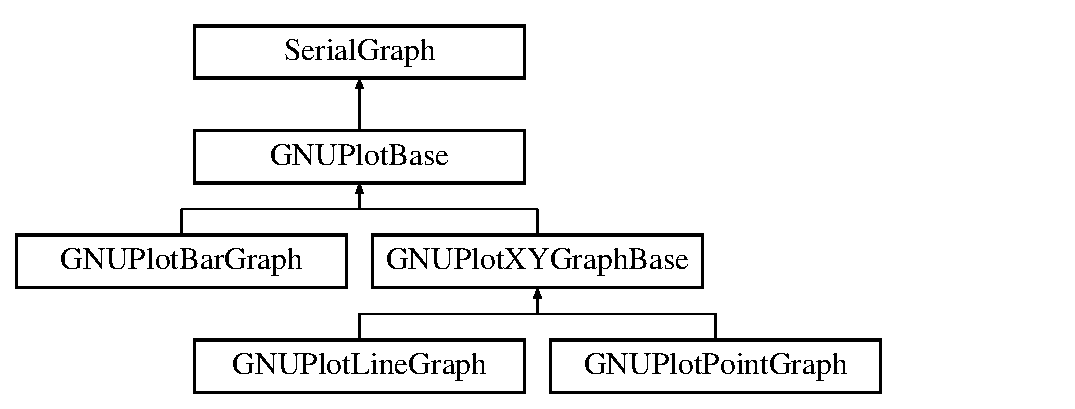
\includegraphics[height=4.000000cm]{class_g_n_u_plot_base}
\end{center}
\end{figure}
\subsection*{Public Member Functions}
\begin{DoxyCompactItemize}
\item 
\hyperlink{class_g_n_u_plot_base_aee6453a84c4357b1fcde2f14b455423f}{G\+N\+U\+Plot\+Base} (Print $\ast$\+\_\+out\+Stream)
\item 
virtual \hyperlink{class_g_n_u_plot_base_abca2da63bc2e235c11d6bca89a954f6d}{$\sim$\+G\+N\+U\+Plot\+Base} ()
\item 
virtual void \hyperlink{class_g_n_u_plot_base_a4d4da234cfdeb99ec3228ef7b2df8a50}{new\+Graph} ()
\item 
virtual void \hyperlink{class_g_n_u_plot_base_aa4b0574c35fbee4dc5f25451eaf956dd}{finish\+Graph} ()
\item 
virtual void \hyperlink{class_g_n_u_plot_base_a219601bd41203477ae73a18d18dd7443}{print\+Comment\+Start} ()
\item 
virtual \hyperlink{_serial_graph_8h_adc73bce6b7e6c4ecf37dde452d6a385e}{Graph\+Style} \hyperlink{class_serial_graph_a2ab97096fffdf429bfa271b9fd4c642a}{get\+Graph\+Style} () const  =0
\item 
virtual void \hyperlink{class_serial_graph_a28b020807c52c113685aa6a31f836c52}{enable\+Save\+Image\+File} (bool enabled)
\item 
virtual void \hyperlink{class_serial_graph_abf488e449d6d786bc01478793d0094ad}{set\+Show\+Grid} (bool enabled)
\item 
void \hyperlink{class_serial_graph_a4db09b008589914b71b2ee8b1873db7a}{set\+Title} (const \+\_\+\+\_\+\+Flash\+String\+Helper $\ast$title)
\item 
virtual void \hyperlink{class_serial_graph_ad726b2c84cec50c2d4bfe769e62a9bcd}{set\+Title} (const char $\ast$title)
\item 
void \hyperlink{class_serial_graph_afdb759a860c41de2fc4cfe78519b9fc0}{set\+X\+Axis\+Name} (const \+\_\+\+\_\+\+Flash\+String\+Helper $\ast$title)
\item 
virtual void \hyperlink{class_serial_graph_ac7f30036f5006091af51204a4d9efaf2}{set\+X\+Axis\+Name} (const char $\ast$name)
\item 
void \hyperlink{class_serial_graph_abfc46c15cf8e1b4362a7f51cb11c7bdb}{set\+Y\+Axis\+Name} (const \+\_\+\+\_\+\+Flash\+String\+Helper $\ast$title)
\item 
virtual void \hyperlink{class_serial_graph_ab0c675c8682959261f79dcf37b04148c}{set\+Y\+Axis\+Name} (const char $\ast$name)
\item 
virtual void \hyperlink{class_serial_graph_ae58de4fa4d391f1a2f411ce00dd74d93}{set\+X\+Axis\+Log} (byte scale)
\item 
virtual void \hyperlink{class_serial_graph_a444e38e8ef3784942ca6ee58940f7023}{set\+Y\+Axis\+Log} (byte scale)
\item 
void \hyperlink{class_serial_graph_a84d8e8ce9bff20e53ba738d1d34d3577}{set\+Series\+Name} (int \+\_\+n, const \+\_\+\+\_\+\+Flash\+String\+Helper $\ast$title)
\item 
virtual void \hyperlink{class_serial_graph_a9d67fbecbee6edb82646aa7ba5103046}{set\+Series\+Name} (int \+\_\+n, const char $\ast$name)
\item 
\hyperlink{struct_line_apperance}{Line\+Apperance} $\ast$ \hyperlink{class_serial_graph_a5a6008dc86a2101a58782929721a5b77}{get\+Line\+Apperance} (int \+\_\+n)
\item 
{\footnotesize template$<$typename Y\+T $>$ }\\void \hyperlink{class_serial_graph_afbcc26bd6bad7179d75379ac0f0d25f1}{plot\+Datum\+Y} (Y\+T y1)
\item 
{\footnotesize template$<$typename X\+T , typename Y\+T $>$ }\\void \hyperlink{class_serial_graph_a265b48fb0afe543e14cedb6619e3931e}{plot\+Datum\+X\+Y} (X\+T x, Y\+T y1)
\item 
{\footnotesize template$<$typename Y\+T $>$ }\\void \hyperlink{class_serial_graph_a56f584fa6316175bc9fbcb4f671f1c93}{plot\+Datum\+Yn} (Y\+T y1, Y\+T y2)
\item 
{\footnotesize template$<$typename Y\+T $>$ }\\void \hyperlink{class_serial_graph_ae755b026606e34c33c4aa8f10d8b5d9c}{plot\+Datum\+Yn} (Y\+T y1, Y\+T y2, Y\+T y3)
\item 
{\footnotesize template$<$typename Y\+T $>$ }\\void \hyperlink{class_serial_graph_a354feb95f91239699d3510c2ce5659b0}{plot\+Datum\+Yn} (Y\+T y1, Y\+T y2, Y\+T y3, Y\+T y4)
\item 
{\footnotesize template$<$typename Y\+T $>$ }\\void \hyperlink{class_serial_graph_ab0fff3fc1879e1cd6aadf24c913ff617}{plot\+Datum\+Yn} (Y\+T y1, Y\+T y2, Y\+T y3, Y\+T y4, Y\+T y5)
\item 
{\footnotesize template$<$typename X\+T , typename Y\+T $>$ }\\void \hyperlink{class_serial_graph_aa20b03efac52c18c50efc79c6459a9fc}{plot\+Datum\+Yn} (const Y\+T $\ast$y\+Vec, int \+\_\+n)
\item 
{\footnotesize template$<$typename X\+T , typename Y\+T $>$ }\\void \hyperlink{class_serial_graph_a79b721ca2be68969862869f96d6a6305}{plot\+Datum\+X\+Yn} (X\+T x, Y\+T y1, Y\+T y2)
\item 
{\footnotesize template$<$typename X\+T , typename Y\+T $>$ }\\void \hyperlink{class_serial_graph_a9fcea879f299a7d24be4ff9a38c53c26}{plot\+Datum\+X\+Yn} (X\+T x, Y\+T y1, Y\+T y2, Y\+T y3)
\item 
{\footnotesize template$<$typename X\+T , typename Y\+T $>$ }\\void \hyperlink{class_serial_graph_afd854b631604abe2014a1bb1beeeec52}{plot\+Datum\+X\+Yn} (X\+T x, Y\+T y1, Y\+T y2, Y\+T y3, Y\+T y4)
\item 
{\footnotesize template$<$typename X\+T , typename Y\+T $>$ }\\void \hyperlink{class_serial_graph_aa1bb6fa08a8bd06c074ac2a02b3f6fbc}{plot\+Datum\+X\+Yn} (X\+T x, Y\+T y1, Y\+T y2, Y\+T y3, Y\+T y4, Y\+T y5)
\item 
{\footnotesize template$<$typename X\+T , typename Y\+T $>$ }\\void \hyperlink{class_serial_graph_a3d7276c89235dc1aa176e2439ad9835b}{plot\+Datum\+X\+Yn} (X\+T x, const Y\+T $\ast$y\+Vec, int \+\_\+n)
\item 
{\footnotesize template$<$typename W\+T $>$ }\\void \hyperlink{class_serial_graph_aa72b48968e82a953dcdc6522bd04c7b4}{print} (const W\+T what)
\item 
{\footnotesize template$<$typename W\+T $>$ }\\void \hyperlink{class_serial_graph_a2005d103cb5a578053ef7838b3a8422d}{println} (const W\+T what)
\item 
{\footnotesize template$<$typename W\+T $>$ }\\void \hyperlink{class_serial_graph_a7237d928f67a14d5c9950d8c23c2a794}{print\+Comment} (const W\+T what)
\item 
{\footnotesize template$<$typename W\+T $>$ }\\void \hyperlink{class_serial_graph_a9b40aa22335fc26a6c29b16d278b26f8}{print\+Comment} (const W\+T $\ast$what)
\end{DoxyCompactItemize}
\subsection*{Public Attributes}
\begin{DoxyCompactItemize}
\item 
const byte \hyperlink{class_serial_graph_a1867ab3a93268646490fa7ba4f8b5680}{max\+String\+Size} = 128
\item 
const byte \hyperlink{class_serial_graph_a752a1429bd35687163fe11c5a2562bef}{max\+Series} = 8
\end{DoxyCompactItemize}
\subsection*{Protected Member Functions}
\begin{DoxyCompactItemize}
\item 
{\footnotesize template$<$typename T , typename U $>$ }\\void \hyperlink{class_g_n_u_plot_base_a03d371b0c6c7ef89064525438b22d52c}{set\+Variable} (T name, U value, bool quoted)
\item 
{\footnotesize template$<$typename T $>$ }\\void \hyperlink{class_g_n_u_plot_base_a3c8c8f68c13661d91bd844589e1a2a85}{set\+Variable} (T name)
\item 
{\footnotesize template$<$typename T $>$ }\\void \hyperlink{class_g_n_u_plot_base_af9b418bbcafb41d4d51b92018ca4f217}{unset\+Variable} (T name)
\item 
{\footnotesize template$<$typename T $>$ }\\void \hyperlink{class_g_n_u_plot_base_a68171bf36461e54e2b81384c112ad975}{set\+Varible\+By\+String\+\_\+null\+Safe} (T name, const char $\ast$text)
\item 
{\footnotesize template$<$typename T $>$ }\\void \hyperlink{class_g_n_u_plot_base_ae93c5de3241c2b6b6f703a202dc1d94b}{set\+Varible\+Flag\+By\+Boolean} (T name, bool value)
\item 
void \hyperlink{class_g_n_u_plot_base_ab5c851953dd140cc3ee936a5cd329200}{save\+Plot\+To\+Image\+File} (const char $\ast$title)
\item 
virtual void \hyperlink{class_g_n_u_plot_base_adaf91c191e4d889537d401faeb863485}{make\+Ready\+For\+Plot\+Data} ()
\item 
char $\ast$ \hyperlink{class_g_n_u_plot_base_a7f71f3c616b3a4a854f9118a04c40447}{malloc\+Basic\+File\+Name\+From\+Graph\+Title} ()
\item 
virtual void \hyperlink{class_g_n_u_plot_base_ad877f207d43e6f9cd0aa0ef241e31c24}{create\+Graph} ()=0
\item 
void \hyperlink{class_g_n_u_plot_base_a65ae2b3220034bce21c7feb39a632991}{print\+Title\+In\+Plot\+Command} (int series\+Num)
\item 
void \hyperlink{class_g_n_u_plot_base_ad057969aa7f8bdbe884d6a5d03a29722}{print\+Line\+Apperance} (\hyperlink{struct_line_apperance}{Line\+Apperance} apperance)
\item 
void \hyperlink{class_g_n_u_plot_base_ad7e8ef8d8e5eb80119fc0cce9be2d525}{print\+Log\+Axis\+Command} (const \+\_\+\+\_\+\+Flash\+String\+Helper $\ast$axis\+Name, byte log\+Scale)
\item 
virtual void \hyperlink{class_g_n_u_plot_base_ae204818b4e8dcd9d2f6b5426127ca2cf}{print\+Seperator} ()
\item 
virtual void \hyperlink{class_g_n_u_plot_base_ac2b48b822b6043392b514c9580b1661a}{print\+Start\+Datum} ()
\item 
virtual void \hyperlink{class_g_n_u_plot_base_aff02bc279e6c3cb83f2cdc7aa021268f}{print\+End\+Datum} ()
\item 
virtual void \hyperlink{class_g_n_u_plot_base_ad00a12fd681e4638fae005891fd72f38}{\+\_\+print\+Data\+Value} (const char $\ast$value)
\item 
virtual void \hyperlink{class_g_n_u_plot_base_aa6c6dfff0568dd99c0c28081c41b4433}{\+\_\+print\+Data\+Value} (char value)
\item 
virtual void \hyperlink{class_g_n_u_plot_base_a6f14fc040ff833c685ab09fc7917e059}{\+\_\+print\+Data\+Value} (bool value)
\item 
void \hyperlink{class_serial_graph_a760dd00474c9780c81ece7cdf621fc15}{init} ()
\item 
void \hyperlink{class_serial_graph_abd43150abedec26eef3994cd33035173}{ensure\+Ready\+To\+Recive\+Plot\+Data} ()
\item 
{\footnotesize template$<$typename T $>$ }\\void \hyperlink{class_serial_graph_a91e20c05c8cc612fd9ffd85880149264}{print\+Data\+Value} (T value)
\item 
virtual void \hyperlink{class_serial_graph_a0c4d2c1239de3107d7332389183b05a1}{\+\_\+print\+Data\+Value} (const \+\_\+\+\_\+\+Flash\+String\+Helper $\ast$value)
\item 
virtual void \hyperlink{class_serial_graph_a58edf4683c600b6bfa1714b0f8dfc82c}{\+\_\+print\+Data\+Value} (int value)
\item 
virtual void \hyperlink{class_serial_graph_a9a4903d4fa26bb85ba5dd93c4365bcc2}{\+\_\+print\+Data\+Value} (long value)
\item 
virtual void \hyperlink{class_serial_graph_acada5333b96b65e31d8c76c3ab22905f}{\+\_\+print\+Data\+Value} (byte value)
\item 
virtual void \hyperlink{class_serial_graph_acd91cf0c3a0f49d4bdf18b447503da23}{\+\_\+print\+Data\+Value} (unsigned int value)
\item 
virtual void \hyperlink{class_serial_graph_a6dbfe61ee398e18c1b752a3748df9663}{\+\_\+print\+Data\+Value} (unsigned long value)
\item 
virtual void \hyperlink{class_serial_graph_a766d5838ede9c8fa998ce8664e5f92be}{\+\_\+print\+Data\+Value} (double value)
\end{DoxyCompactItemize}
\subsection*{Protected Attributes}
\begin{DoxyCompactItemize}
\item 
bool \hyperlink{class_serial_graph_a24202e0a7a8bac5ec1cfd92bf796e078}{save\+File}
\item 
Print $\ast$ \hyperlink{class_serial_graph_aec32289a9393e98bf80d44406e5c207d}{out\+Stream}
\item 
bool \hyperlink{class_serial_graph_a4dbd9cf190c591fb4f2f46a50d937199}{x\+Axis\+Specified}
\item 
int \hyperlink{class_serial_graph_ab40c430e06102b9624736173d4a58596}{num\+Y\+Series}
\item 
bool \hyperlink{class_serial_graph_ad61d5ea29eacc1611c5addc94714f1e2}{show\+Grid}
\item 
char $\ast$ \hyperlink{class_serial_graph_a0b33d43c2bb54340ef1f90b5f76d7aea}{graph\+Title}
\item 
char $\ast$ \hyperlink{class_serial_graph_a5f5bf85ed361ff567d0888eaa73e269c}{x\+Axis\+Name}
\item 
char $\ast$ \hyperlink{class_serial_graph_a08452a56c74ec5f5473b64605d555339}{y\+Axis\+Name}
\item 
char $\ast$$\ast$ \hyperlink{class_serial_graph_a2307e40e27249f44bbe14776dc68c561}{series\+Names}
\item 
\hyperlink{struct_line_apperance}{Line\+Apperance} $\ast$ \hyperlink{class_serial_graph_a8d743f9eeeca69a988d2159a405e4253}{series\+Apperance}
\item 
byte \hyperlink{class_serial_graph_afc2ca72fdfe2bc5e3159c9e910a8f81e}{x\+Axis\+Log\+Scale}
\item 
byte \hyperlink{class_serial_graph_a1f0424857ec14c176747b3ddb0768eee}{y\+Axis\+Log\+Scale}
\end{DoxyCompactItemize}


\subsection{Detailed Description}
A base class for all things G\+N\+U plot. 

\subsection{Constructor \& Destructor Documentation}
\hypertarget{class_g_n_u_plot_base_aee6453a84c4357b1fcde2f14b455423f}{}\index{G\+N\+U\+Plot\+Base@{G\+N\+U\+Plot\+Base}!G\+N\+U\+Plot\+Base@{G\+N\+U\+Plot\+Base}}
\index{G\+N\+U\+Plot\+Base@{G\+N\+U\+Plot\+Base}!G\+N\+U\+Plot\+Base@{G\+N\+U\+Plot\+Base}}
\subsubsection[{G\+N\+U\+Plot\+Base(\+Print $\ast$\+\_\+out\+Stream)}]{\setlength{\rightskip}{0pt plus 5cm}G\+N\+U\+Plot\+Base\+::\+G\+N\+U\+Plot\+Base (
\begin{DoxyParamCaption}
\item[{Print $\ast$}]{\+\_\+out\+Stream}
\end{DoxyParamCaption}
)\hspace{0.3cm}{\ttfamily [inline]}}\label{class_g_n_u_plot_base_aee6453a84c4357b1fcde2f14b455423f}
\hypertarget{class_g_n_u_plot_base_abca2da63bc2e235c11d6bca89a954f6d}{}\index{G\+N\+U\+Plot\+Base@{G\+N\+U\+Plot\+Base}!````~G\+N\+U\+Plot\+Base@{$\sim$\+G\+N\+U\+Plot\+Base}}
\index{````~G\+N\+U\+Plot\+Base@{$\sim$\+G\+N\+U\+Plot\+Base}!G\+N\+U\+Plot\+Base@{G\+N\+U\+Plot\+Base}}
\subsubsection[{$\sim$\+G\+N\+U\+Plot\+Base()}]{\setlength{\rightskip}{0pt plus 5cm}virtual G\+N\+U\+Plot\+Base\+::$\sim$\+G\+N\+U\+Plot\+Base (
\begin{DoxyParamCaption}
{}
\end{DoxyParamCaption}
)\hspace{0.3cm}{\ttfamily [inline]}, {\ttfamily [virtual]}}\label{class_g_n_u_plot_base_abca2da63bc2e235c11d6bca89a954f6d}


\subsection{Member Function Documentation}
\hypertarget{class_g_n_u_plot_base_ad00a12fd681e4638fae005891fd72f38}{}\index{G\+N\+U\+Plot\+Base@{G\+N\+U\+Plot\+Base}!\+\_\+print\+Data\+Value@{\+\_\+print\+Data\+Value}}
\index{\+\_\+print\+Data\+Value@{\+\_\+print\+Data\+Value}!G\+N\+U\+Plot\+Base@{G\+N\+U\+Plot\+Base}}
\subsubsection[{\+\_\+print\+Data\+Value(const char $\ast$value)}]{\setlength{\rightskip}{0pt plus 5cm}void G\+N\+U\+Plot\+Base\+::\+\_\+print\+Data\+Value (
\begin{DoxyParamCaption}
\item[{const char $\ast$}]{value}
\end{DoxyParamCaption}
)\hspace{0.3cm}{\ttfamily [protected]}, {\ttfamily [virtual]}}\label{class_g_n_u_plot_base_ad00a12fd681e4638fae005891fd72f38}
Override a put appropriate quotes around strings etc. 
\begin{DoxyParams}{Parameters}
{\em value} & What to print. \\
\hline
\end{DoxyParams}


Reimplemented from \hyperlink{class_serial_graph_a8252997dd4bad0251d437d6dd097bffb}{Serial\+Graph}.

\hypertarget{class_g_n_u_plot_base_aa6c6dfff0568dd99c0c28081c41b4433}{}\index{G\+N\+U\+Plot\+Base@{G\+N\+U\+Plot\+Base}!\+\_\+print\+Data\+Value@{\+\_\+print\+Data\+Value}}
\index{\+\_\+print\+Data\+Value@{\+\_\+print\+Data\+Value}!G\+N\+U\+Plot\+Base@{G\+N\+U\+Plot\+Base}}
\subsubsection[{\+\_\+print\+Data\+Value(char value)}]{\setlength{\rightskip}{0pt plus 5cm}virtual void G\+N\+U\+Plot\+Base\+::\+\_\+print\+Data\+Value (
\begin{DoxyParamCaption}
\item[{char}]{value}
\end{DoxyParamCaption}
)\hspace{0.3cm}{\ttfamily [inline]}, {\ttfamily [protected]}, {\ttfamily [virtual]}}\label{class_g_n_u_plot_base_aa6c6dfff0568dd99c0c28081c41b4433}
Override for customised value output. 
\begin{DoxyParams}{Parameters}
{\em value} & What to print. \\
\hline
\end{DoxyParams}


Reimplemented from \hyperlink{class_serial_graph_af3fbf7a9201f71cd6bad7e4337092fb6}{Serial\+Graph}.

\hypertarget{class_g_n_u_plot_base_a6f14fc040ff833c685ab09fc7917e059}{}\index{G\+N\+U\+Plot\+Base@{G\+N\+U\+Plot\+Base}!\+\_\+print\+Data\+Value@{\+\_\+print\+Data\+Value}}
\index{\+\_\+print\+Data\+Value@{\+\_\+print\+Data\+Value}!G\+N\+U\+Plot\+Base@{G\+N\+U\+Plot\+Base}}
\subsubsection[{\+\_\+print\+Data\+Value(bool value)}]{\setlength{\rightskip}{0pt plus 5cm}virtual void G\+N\+U\+Plot\+Base\+::\+\_\+print\+Data\+Value (
\begin{DoxyParamCaption}
\item[{bool}]{value}
\end{DoxyParamCaption}
)\hspace{0.3cm}{\ttfamily [inline]}, {\ttfamily [protected]}, {\ttfamily [virtual]}}\label{class_g_n_u_plot_base_a6f14fc040ff833c685ab09fc7917e059}
Override for customised value output. 
\begin{DoxyParams}{Parameters}
{\em value} & What to print. \\
\hline
\end{DoxyParams}


Reimplemented from \hyperlink{class_serial_graph_aed9ff95634ace3d190863ea9d15c10da}{Serial\+Graph}.

\hypertarget{class_serial_graph_a0c4d2c1239de3107d7332389183b05a1}{}\index{G\+N\+U\+Plot\+Base@{G\+N\+U\+Plot\+Base}!\+\_\+print\+Data\+Value@{\+\_\+print\+Data\+Value}}
\index{\+\_\+print\+Data\+Value@{\+\_\+print\+Data\+Value}!G\+N\+U\+Plot\+Base@{G\+N\+U\+Plot\+Base}}
\subsubsection[{\+\_\+print\+Data\+Value(const \+\_\+\+\_\+\+Flash\+String\+Helper $\ast$value)}]{\setlength{\rightskip}{0pt plus 5cm}virtual void Serial\+Graph\+::\+\_\+print\+Data\+Value (
\begin{DoxyParamCaption}
\item[{const \+\_\+\+\_\+\+Flash\+String\+Helper $\ast$}]{value}
\end{DoxyParamCaption}
)\hspace{0.3cm}{\ttfamily [inline]}, {\ttfamily [protected]}, {\ttfamily [virtual]}, {\ttfamily [inherited]}}\label{class_serial_graph_a0c4d2c1239de3107d7332389183b05a1}
This just calls \hyperlink{class_serial_graph_a8252997dd4bad0251d437d6dd097bffb}{\+\_\+print\+Data\+Value(const char $\ast$value)} so probably alter that instead. 
\begin{DoxyParams}{Parameters}
{\em value} & What to print. \\
\hline
\end{DoxyParams}
\hypertarget{class_serial_graph_a58edf4683c600b6bfa1714b0f8dfc82c}{}\index{G\+N\+U\+Plot\+Base@{G\+N\+U\+Plot\+Base}!\+\_\+print\+Data\+Value@{\+\_\+print\+Data\+Value}}
\index{\+\_\+print\+Data\+Value@{\+\_\+print\+Data\+Value}!G\+N\+U\+Plot\+Base@{G\+N\+U\+Plot\+Base}}
\subsubsection[{\+\_\+print\+Data\+Value(int value)}]{\setlength{\rightskip}{0pt plus 5cm}virtual void Serial\+Graph\+::\+\_\+print\+Data\+Value (
\begin{DoxyParamCaption}
\item[{int}]{value}
\end{DoxyParamCaption}
)\hspace{0.3cm}{\ttfamily [inline]}, {\ttfamily [protected]}, {\ttfamily [virtual]}, {\ttfamily [inherited]}}\label{class_serial_graph_a58edf4683c600b6bfa1714b0f8dfc82c}
Override for customised value output. 
\begin{DoxyParams}{Parameters}
{\em value} & What to print. \\
\hline
\end{DoxyParams}
\hypertarget{class_serial_graph_a9a4903d4fa26bb85ba5dd93c4365bcc2}{}\index{G\+N\+U\+Plot\+Base@{G\+N\+U\+Plot\+Base}!\+\_\+print\+Data\+Value@{\+\_\+print\+Data\+Value}}
\index{\+\_\+print\+Data\+Value@{\+\_\+print\+Data\+Value}!G\+N\+U\+Plot\+Base@{G\+N\+U\+Plot\+Base}}
\subsubsection[{\+\_\+print\+Data\+Value(long value)}]{\setlength{\rightskip}{0pt plus 5cm}virtual void Serial\+Graph\+::\+\_\+print\+Data\+Value (
\begin{DoxyParamCaption}
\item[{long}]{value}
\end{DoxyParamCaption}
)\hspace{0.3cm}{\ttfamily [inline]}, {\ttfamily [protected]}, {\ttfamily [virtual]}, {\ttfamily [inherited]}}\label{class_serial_graph_a9a4903d4fa26bb85ba5dd93c4365bcc2}
Override for customised value output. 
\begin{DoxyParams}{Parameters}
{\em value} & What to print. \\
\hline
\end{DoxyParams}
\hypertarget{class_serial_graph_acada5333b96b65e31d8c76c3ab22905f}{}\index{G\+N\+U\+Plot\+Base@{G\+N\+U\+Plot\+Base}!\+\_\+print\+Data\+Value@{\+\_\+print\+Data\+Value}}
\index{\+\_\+print\+Data\+Value@{\+\_\+print\+Data\+Value}!G\+N\+U\+Plot\+Base@{G\+N\+U\+Plot\+Base}}
\subsubsection[{\+\_\+print\+Data\+Value(byte value)}]{\setlength{\rightskip}{0pt plus 5cm}virtual void Serial\+Graph\+::\+\_\+print\+Data\+Value (
\begin{DoxyParamCaption}
\item[{byte}]{value}
\end{DoxyParamCaption}
)\hspace{0.3cm}{\ttfamily [inline]}, {\ttfamily [protected]}, {\ttfamily [virtual]}, {\ttfamily [inherited]}}\label{class_serial_graph_acada5333b96b65e31d8c76c3ab22905f}
Override for customised value output. 
\begin{DoxyParams}{Parameters}
{\em value} & What to print. \\
\hline
\end{DoxyParams}
\hypertarget{class_serial_graph_acd91cf0c3a0f49d4bdf18b447503da23}{}\index{G\+N\+U\+Plot\+Base@{G\+N\+U\+Plot\+Base}!\+\_\+print\+Data\+Value@{\+\_\+print\+Data\+Value}}
\index{\+\_\+print\+Data\+Value@{\+\_\+print\+Data\+Value}!G\+N\+U\+Plot\+Base@{G\+N\+U\+Plot\+Base}}
\subsubsection[{\+\_\+print\+Data\+Value(unsigned int value)}]{\setlength{\rightskip}{0pt plus 5cm}virtual void Serial\+Graph\+::\+\_\+print\+Data\+Value (
\begin{DoxyParamCaption}
\item[{unsigned int}]{value}
\end{DoxyParamCaption}
)\hspace{0.3cm}{\ttfamily [inline]}, {\ttfamily [protected]}, {\ttfamily [virtual]}, {\ttfamily [inherited]}}\label{class_serial_graph_acd91cf0c3a0f49d4bdf18b447503da23}
Override for customised value output. 
\begin{DoxyParams}{Parameters}
{\em value} & What to print. \\
\hline
\end{DoxyParams}
\hypertarget{class_serial_graph_a6dbfe61ee398e18c1b752a3748df9663}{}\index{G\+N\+U\+Plot\+Base@{G\+N\+U\+Plot\+Base}!\+\_\+print\+Data\+Value@{\+\_\+print\+Data\+Value}}
\index{\+\_\+print\+Data\+Value@{\+\_\+print\+Data\+Value}!G\+N\+U\+Plot\+Base@{G\+N\+U\+Plot\+Base}}
\subsubsection[{\+\_\+print\+Data\+Value(unsigned long value)}]{\setlength{\rightskip}{0pt plus 5cm}virtual void Serial\+Graph\+::\+\_\+print\+Data\+Value (
\begin{DoxyParamCaption}
\item[{unsigned long}]{value}
\end{DoxyParamCaption}
)\hspace{0.3cm}{\ttfamily [inline]}, {\ttfamily [protected]}, {\ttfamily [virtual]}, {\ttfamily [inherited]}}\label{class_serial_graph_a6dbfe61ee398e18c1b752a3748df9663}
Override for customised value output. 
\begin{DoxyParams}{Parameters}
{\em value} & What to print. \\
\hline
\end{DoxyParams}
\hypertarget{class_serial_graph_a766d5838ede9c8fa998ce8664e5f92be}{}\index{G\+N\+U\+Plot\+Base@{G\+N\+U\+Plot\+Base}!\+\_\+print\+Data\+Value@{\+\_\+print\+Data\+Value}}
\index{\+\_\+print\+Data\+Value@{\+\_\+print\+Data\+Value}!G\+N\+U\+Plot\+Base@{G\+N\+U\+Plot\+Base}}
\subsubsection[{\+\_\+print\+Data\+Value(double value)}]{\setlength{\rightskip}{0pt plus 5cm}virtual void Serial\+Graph\+::\+\_\+print\+Data\+Value (
\begin{DoxyParamCaption}
\item[{double}]{value}
\end{DoxyParamCaption}
)\hspace{0.3cm}{\ttfamily [inline]}, {\ttfamily [protected]}, {\ttfamily [virtual]}, {\ttfamily [inherited]}}\label{class_serial_graph_a766d5838ede9c8fa998ce8664e5f92be}
Override for customised value output. 
\begin{DoxyParams}{Parameters}
{\em value} & What to print. \\
\hline
\end{DoxyParams}
\hypertarget{class_g_n_u_plot_base_ad877f207d43e6f9cd0aa0ef241e31c24}{}\index{G\+N\+U\+Plot\+Base@{G\+N\+U\+Plot\+Base}!create\+Graph@{create\+Graph}}
\index{create\+Graph@{create\+Graph}!G\+N\+U\+Plot\+Base@{G\+N\+U\+Plot\+Base}}
\subsubsection[{create\+Graph()=0}]{\setlength{\rightskip}{0pt plus 5cm}virtual void G\+N\+U\+Plot\+Base\+::create\+Graph (
\begin{DoxyParamCaption}
{}
\end{DoxyParamCaption}
)\hspace{0.3cm}{\ttfamily [protected]}, {\ttfamily [pure virtual]}}\label{class_g_n_u_plot_base_ad877f207d43e6f9cd0aa0ef241e31c24}


Implemented in \hyperlink{class_g_n_u_plot_bar_graph_a89a417ec362ccfcaeb23db8438d3579e}{G\+N\+U\+Plot\+Bar\+Graph}, and \hyperlink{class_g_n_u_plot_x_y_graph_base_a8389f830ff330dfb705e00d31053e130}{G\+N\+U\+Plot\+X\+Y\+Graph\+Base}.

\hypertarget{class_serial_graph_a28b020807c52c113685aa6a31f836c52}{}\index{G\+N\+U\+Plot\+Base@{G\+N\+U\+Plot\+Base}!enable\+Save\+Image\+File@{enable\+Save\+Image\+File}}
\index{enable\+Save\+Image\+File@{enable\+Save\+Image\+File}!G\+N\+U\+Plot\+Base@{G\+N\+U\+Plot\+Base}}
\subsubsection[{enable\+Save\+Image\+File(bool enabled)}]{\setlength{\rightskip}{0pt plus 5cm}virtual void Serial\+Graph\+::enable\+Save\+Image\+File (
\begin{DoxyParamCaption}
\item[{bool}]{enabled}
\end{DoxyParamCaption}
)\hspace{0.3cm}{\ttfamily [inline]}, {\ttfamily [virtual]}, {\ttfamily [inherited]}}\label{class_serial_graph_a28b020807c52c113685aa6a31f836c52}
Set to true if an image file should be saved. \begin{DoxyNote}{Note}
Filename will be based on graph title. This is done to save memory. Final filename has some extra validation performed to conform with filename rules aplicable to modern operating systems (excluding 8 char limit). 
\end{DoxyNote}
\hypertarget{class_serial_graph_abd43150abedec26eef3994cd33035173}{}\index{G\+N\+U\+Plot\+Base@{G\+N\+U\+Plot\+Base}!ensure\+Ready\+To\+Recive\+Plot\+Data@{ensure\+Ready\+To\+Recive\+Plot\+Data}}
\index{ensure\+Ready\+To\+Recive\+Plot\+Data@{ensure\+Ready\+To\+Recive\+Plot\+Data}!G\+N\+U\+Plot\+Base@{G\+N\+U\+Plot\+Base}}
\subsubsection[{ensure\+Ready\+To\+Recive\+Plot\+Data()}]{\setlength{\rightskip}{0pt plus 5cm}void Serial\+Graph\+::ensure\+Ready\+To\+Recive\+Plot\+Data (
\begin{DoxyParamCaption}
{}
\end{DoxyParamCaption}
)\hspace{0.3cm}{\ttfamily [protected]}, {\ttfamily [inherited]}}\label{class_serial_graph_abd43150abedec26eef3994cd33035173}
Called by every plot command prior to sending data. it\textquotesingle{}s function is to call \hyperlink{class_serial_graph_a898cf274c886e0ff45e90d3f21f0a6cc}{make\+Ready\+For\+Plot\+Data()} the first time it is called. 
\begin{DoxyParams}{Parameters}
{\em value} & What to print. \\
\hline
\end{DoxyParams}
\hypertarget{class_g_n_u_plot_base_aa4b0574c35fbee4dc5f25451eaf956dd}{}\index{G\+N\+U\+Plot\+Base@{G\+N\+U\+Plot\+Base}!finish\+Graph@{finish\+Graph}}
\index{finish\+Graph@{finish\+Graph}!G\+N\+U\+Plot\+Base@{G\+N\+U\+Plot\+Base}}
\subsubsection[{finish\+Graph()}]{\setlength{\rightskip}{0pt plus 5cm}void G\+N\+U\+Plot\+Base\+::finish\+Graph (
\begin{DoxyParamCaption}
{}
\end{DoxyParamCaption}
)\hspace{0.3cm}{\ttfamily [virtual]}}\label{class_g_n_u_plot_base_aa4b0574c35fbee4dc5f25451eaf956dd}
Serial output that finishes the plot, saves file, updates display etc. 

Implements \hyperlink{class_serial_graph_a8054ce989a1788bd35d2fde56081c88c}{Serial\+Graph}.

\hypertarget{class_serial_graph_a2ab97096fffdf429bfa271b9fd4c642a}{}\index{G\+N\+U\+Plot\+Base@{G\+N\+U\+Plot\+Base}!get\+Graph\+Style@{get\+Graph\+Style}}
\index{get\+Graph\+Style@{get\+Graph\+Style}!G\+N\+U\+Plot\+Base@{G\+N\+U\+Plot\+Base}}
\subsubsection[{get\+Graph\+Style() const  =0}]{\setlength{\rightskip}{0pt plus 5cm}virtual {\bf Graph\+Style} Serial\+Graph\+::get\+Graph\+Style (
\begin{DoxyParamCaption}
{}
\end{DoxyParamCaption}
) const\hspace{0.3cm}{\ttfamily [pure virtual]}, {\ttfamily [inherited]}}\label{class_serial_graph_a2ab97096fffdf429bfa271b9fd4c642a}
Returns the Graph\+Style of the current object. 

Implemented in \hyperlink{class_g_n_u_plot_bar_graph_a6b2cde2832fcb246361d8ebddbe7a228}{G\+N\+U\+Plot\+Bar\+Graph}, \hyperlink{class_g_n_u_plot_point_graph_aeeae395426112202d3617ff66d836c99}{G\+N\+U\+Plot\+Point\+Graph}, and \hyperlink{class_g_n_u_plot_line_graph_a8f8b19efd8d8f4f25ccc41635e332593}{G\+N\+U\+Plot\+Line\+Graph}.

\hypertarget{class_serial_graph_a5a6008dc86a2101a58782929721a5b77}{}\index{G\+N\+U\+Plot\+Base@{G\+N\+U\+Plot\+Base}!get\+Line\+Apperance@{get\+Line\+Apperance}}
\index{get\+Line\+Apperance@{get\+Line\+Apperance}!G\+N\+U\+Plot\+Base@{G\+N\+U\+Plot\+Base}}
\subsubsection[{get\+Line\+Apperance(int \+\_\+n)}]{\setlength{\rightskip}{0pt plus 5cm}{\bf Line\+Apperance}$\ast$ Serial\+Graph\+::get\+Line\+Apperance (
\begin{DoxyParamCaption}
\item[{int}]{\+\_\+n}
\end{DoxyParamCaption}
)\hspace{0.3cm}{\ttfamily [inline]}, {\ttfamily [inherited]}}\label{class_serial_graph_a5a6008dc86a2101a58782929721a5b77}
Gets a structure that controls apperance of a series (called a \hyperlink{struct_line_apperance}{Line\+Apperance}). It is intended that you directly modify the structure returned, there is no set\+Line\+Apperance. See the struct \hyperlink{struct_line_apperance}{Line\+Apperance} for more.


\begin{DoxyParams}{Parameters}
{\em \+\_\+n} & Series number to alter.\\
\hline
\end{DoxyParams}
\begin{DoxyNote}{Note}
Behaviour on \+\_\+n $>$ max\+Series, is to just override the last possible series entry. 
\end{DoxyNote}
\hypertarget{class_serial_graph_a760dd00474c9780c81ece7cdf621fc15}{}\index{G\+N\+U\+Plot\+Base@{G\+N\+U\+Plot\+Base}!init@{init}}
\index{init@{init}!G\+N\+U\+Plot\+Base@{G\+N\+U\+Plot\+Base}}
\subsubsection[{init()}]{\setlength{\rightskip}{0pt plus 5cm}void Serial\+Graph\+::init (
\begin{DoxyParamCaption}
{}
\end{DoxyParamCaption}
)\hspace{0.3cm}{\ttfamily [protected]}, {\ttfamily [inherited]}}\label{class_serial_graph_a760dd00474c9780c81ece7cdf621fc15}
Brings the class to its default state. Called by the constructor and \hyperlink{class_serial_graph_a44d34593c56aa67142ccd9fcc0a1da86}{new\+Graph()}. \hypertarget{class_g_n_u_plot_base_adaf91c191e4d889537d401faeb863485}{}\index{G\+N\+U\+Plot\+Base@{G\+N\+U\+Plot\+Base}!make\+Ready\+For\+Plot\+Data@{make\+Ready\+For\+Plot\+Data}}
\index{make\+Ready\+For\+Plot\+Data@{make\+Ready\+For\+Plot\+Data}!G\+N\+U\+Plot\+Base@{G\+N\+U\+Plot\+Base}}
\subsubsection[{make\+Ready\+For\+Plot\+Data()}]{\setlength{\rightskip}{0pt plus 5cm}void G\+N\+U\+Plot\+Base\+::make\+Ready\+For\+Plot\+Data (
\begin{DoxyParamCaption}
{}
\end{DoxyParamCaption}
)\hspace{0.3cm}{\ttfamily [protected]}, {\ttfamily [virtual]}}\label{class_g_n_u_plot_base_adaf91c191e4d889537d401faeb863485}
Called by ensure\+Ready\+To\+Recive\+Plot\+Data, if the first plot command is encountered. \begin{DoxyNote}{Note}
A concrete class should override this. 
\end{DoxyNote}


Reimplemented from \hyperlink{class_serial_graph_a898cf274c886e0ff45e90d3f21f0a6cc}{Serial\+Graph}.

\hypertarget{class_g_n_u_plot_base_a7f71f3c616b3a4a854f9118a04c40447}{}\index{G\+N\+U\+Plot\+Base@{G\+N\+U\+Plot\+Base}!malloc\+Basic\+File\+Name\+From\+Graph\+Title@{malloc\+Basic\+File\+Name\+From\+Graph\+Title}}
\index{malloc\+Basic\+File\+Name\+From\+Graph\+Title@{malloc\+Basic\+File\+Name\+From\+Graph\+Title}!G\+N\+U\+Plot\+Base@{G\+N\+U\+Plot\+Base}}
\subsubsection[{malloc\+Basic\+File\+Name\+From\+Graph\+Title()}]{\setlength{\rightskip}{0pt plus 5cm}char $\ast$ G\+N\+U\+Plot\+Base\+::malloc\+Basic\+File\+Name\+From\+Graph\+Title (
\begin{DoxyParamCaption}
{}
\end{DoxyParamCaption}
)\hspace{0.3cm}{\ttfamily [protected]}}\label{class_g_n_u_plot_base_a7f71f3c616b3a4a854f9118a04c40447}
\hypertarget{class_g_n_u_plot_base_a4d4da234cfdeb99ec3228ef7b2df8a50}{}\index{G\+N\+U\+Plot\+Base@{G\+N\+U\+Plot\+Base}!new\+Graph@{new\+Graph}}
\index{new\+Graph@{new\+Graph}!G\+N\+U\+Plot\+Base@{G\+N\+U\+Plot\+Base}}
\subsubsection[{new\+Graph()}]{\setlength{\rightskip}{0pt plus 5cm}void G\+N\+U\+Plot\+Base\+::new\+Graph (
\begin{DoxyParamCaption}
{}
\end{DoxyParamCaption}
)\hspace{0.3cm}{\ttfamily [virtual]}}\label{class_g_n_u_plot_base_a4d4da234cfdeb99ec3228ef7b2df8a50}
Serial output that establishes a new graph. This should also call \hyperlink{class_serial_graph_a760dd00474c9780c81ece7cdf621fc15}{init()}, to reset the class. \begin{DoxyNote}{Note}
\+: If you wan\textquotesingle{}t a \char`\"{}memory breather\char`\"{} between plots, calling this method frees all series names, titles etc. 
\end{DoxyNote}


Implements \hyperlink{class_serial_graph_a44d34593c56aa67142ccd9fcc0a1da86}{Serial\+Graph}.

\hypertarget{class_serial_graph_a265b48fb0afe543e14cedb6619e3931e}{}\index{G\+N\+U\+Plot\+Base@{G\+N\+U\+Plot\+Base}!plot\+Datum\+X\+Y@{plot\+Datum\+X\+Y}}
\index{plot\+Datum\+X\+Y@{plot\+Datum\+X\+Y}!G\+N\+U\+Plot\+Base@{G\+N\+U\+Plot\+Base}}
\subsubsection[{plot\+Datum\+X\+Y(\+X\+T x, Y\+T y1)}]{\setlength{\rightskip}{0pt plus 5cm}template$<$typename X\+T , typename Y\+T $>$ void Serial\+Graph\+::plot\+Datum\+X\+Y (
\begin{DoxyParamCaption}
\item[{X\+T}]{x, }
\item[{Y\+T}]{y1}
\end{DoxyParamCaption}
)\hspace{0.3cm}{\ttfamily [inline]}, {\ttfamily [inherited]}}\label{class_serial_graph_a265b48fb0afe543e14cedb6619e3931e}
Outputs a point to be plotted. All Y values must be of the same type.

\begin{DoxyNote}{Note}
The first time this is called after \hyperlink{class_serial_graph_a44d34593c56aa67142ccd9fcc0a1da86}{new\+Graph()}, \hyperlink{class_serial_graph_a898cf274c886e0ff45e90d3f21f0a6cc}{make\+Ready\+For\+Plot\+Data()} will be called. 

The following feilds automatically set\+: x\+Axis\+Specified; num\+Y\+Series; 
\end{DoxyNote}
\hypertarget{class_serial_graph_a79b721ca2be68969862869f96d6a6305}{}\index{G\+N\+U\+Plot\+Base@{G\+N\+U\+Plot\+Base}!plot\+Datum\+X\+Yn@{plot\+Datum\+X\+Yn}}
\index{plot\+Datum\+X\+Yn@{plot\+Datum\+X\+Yn}!G\+N\+U\+Plot\+Base@{G\+N\+U\+Plot\+Base}}
\subsubsection[{plot\+Datum\+X\+Yn(\+X\+T x, Y\+T y1, Y\+T y2)}]{\setlength{\rightskip}{0pt plus 5cm}template$<$typename X\+T , typename Y\+T $>$ void Serial\+Graph\+::plot\+Datum\+X\+Yn (
\begin{DoxyParamCaption}
\item[{X\+T}]{x, }
\item[{Y\+T}]{y1, }
\item[{Y\+T}]{y2}
\end{DoxyParamCaption}
)\hspace{0.3cm}{\ttfamily [inline]}, {\ttfamily [inherited]}}\label{class_serial_graph_a79b721ca2be68969862869f96d6a6305}
Outputs a point to be plotted. All Y values must be of the same type.

\begin{DoxyNote}{Note}
The first time this is called after \hyperlink{class_serial_graph_a44d34593c56aa67142ccd9fcc0a1da86}{new\+Graph()}, \hyperlink{class_serial_graph_a898cf274c886e0ff45e90d3f21f0a6cc}{make\+Ready\+For\+Plot\+Data()} will be called. 

The following feilds automatically set\+: x\+Axis\+Specified; num\+Y\+Series; 
\end{DoxyNote}
\hypertarget{class_serial_graph_a9fcea879f299a7d24be4ff9a38c53c26}{}\index{G\+N\+U\+Plot\+Base@{G\+N\+U\+Plot\+Base}!plot\+Datum\+X\+Yn@{plot\+Datum\+X\+Yn}}
\index{plot\+Datum\+X\+Yn@{plot\+Datum\+X\+Yn}!G\+N\+U\+Plot\+Base@{G\+N\+U\+Plot\+Base}}
\subsubsection[{plot\+Datum\+X\+Yn(\+X\+T x, Y\+T y1, Y\+T y2, Y\+T y3)}]{\setlength{\rightskip}{0pt plus 5cm}template$<$typename X\+T , typename Y\+T $>$ void Serial\+Graph\+::plot\+Datum\+X\+Yn (
\begin{DoxyParamCaption}
\item[{X\+T}]{x, }
\item[{Y\+T}]{y1, }
\item[{Y\+T}]{y2, }
\item[{Y\+T}]{y3}
\end{DoxyParamCaption}
)\hspace{0.3cm}{\ttfamily [inline]}, {\ttfamily [inherited]}}\label{class_serial_graph_a9fcea879f299a7d24be4ff9a38c53c26}
Outputs a point to be plotted. All Y values must be of the same type.

\begin{DoxyNote}{Note}
The first time this is called after \hyperlink{class_serial_graph_a44d34593c56aa67142ccd9fcc0a1da86}{new\+Graph()}, \hyperlink{class_serial_graph_a898cf274c886e0ff45e90d3f21f0a6cc}{make\+Ready\+For\+Plot\+Data()} will be called. 

The following feilds automatically set\+: x\+Axis\+Specified; num\+Y\+Series; 
\end{DoxyNote}
\hypertarget{class_serial_graph_afd854b631604abe2014a1bb1beeeec52}{}\index{G\+N\+U\+Plot\+Base@{G\+N\+U\+Plot\+Base}!plot\+Datum\+X\+Yn@{plot\+Datum\+X\+Yn}}
\index{plot\+Datum\+X\+Yn@{plot\+Datum\+X\+Yn}!G\+N\+U\+Plot\+Base@{G\+N\+U\+Plot\+Base}}
\subsubsection[{plot\+Datum\+X\+Yn(\+X\+T x, Y\+T y1, Y\+T y2, Y\+T y3, Y\+T y4)}]{\setlength{\rightskip}{0pt plus 5cm}template$<$typename X\+T , typename Y\+T $>$ void Serial\+Graph\+::plot\+Datum\+X\+Yn (
\begin{DoxyParamCaption}
\item[{X\+T}]{x, }
\item[{Y\+T}]{y1, }
\item[{Y\+T}]{y2, }
\item[{Y\+T}]{y3, }
\item[{Y\+T}]{y4}
\end{DoxyParamCaption}
)\hspace{0.3cm}{\ttfamily [inline]}, {\ttfamily [inherited]}}\label{class_serial_graph_afd854b631604abe2014a1bb1beeeec52}
Outputs a point to be plotted. All Y values must be of the same type.

\begin{DoxyNote}{Note}
The first time this is called after \hyperlink{class_serial_graph_a44d34593c56aa67142ccd9fcc0a1da86}{new\+Graph()}, \hyperlink{class_serial_graph_a898cf274c886e0ff45e90d3f21f0a6cc}{make\+Ready\+For\+Plot\+Data()} will be called. 

The following feilds automatically set\+: x\+Axis\+Specified; num\+Y\+Series; 
\end{DoxyNote}
\hypertarget{class_serial_graph_aa1bb6fa08a8bd06c074ac2a02b3f6fbc}{}\index{G\+N\+U\+Plot\+Base@{G\+N\+U\+Plot\+Base}!plot\+Datum\+X\+Yn@{plot\+Datum\+X\+Yn}}
\index{plot\+Datum\+X\+Yn@{plot\+Datum\+X\+Yn}!G\+N\+U\+Plot\+Base@{G\+N\+U\+Plot\+Base}}
\subsubsection[{plot\+Datum\+X\+Yn(\+X\+T x, Y\+T y1, Y\+T y2, Y\+T y3, Y\+T y4, Y\+T y5)}]{\setlength{\rightskip}{0pt plus 5cm}template$<$typename X\+T , typename Y\+T $>$ void Serial\+Graph\+::plot\+Datum\+X\+Yn (
\begin{DoxyParamCaption}
\item[{X\+T}]{x, }
\item[{Y\+T}]{y1, }
\item[{Y\+T}]{y2, }
\item[{Y\+T}]{y3, }
\item[{Y\+T}]{y4, }
\item[{Y\+T}]{y5}
\end{DoxyParamCaption}
)\hspace{0.3cm}{\ttfamily [inline]}, {\ttfamily [inherited]}}\label{class_serial_graph_aa1bb6fa08a8bd06c074ac2a02b3f6fbc}
Outputs a point to be plotted. All Y values must be of the same type.

\begin{DoxyNote}{Note}
The first time this is called after \hyperlink{class_serial_graph_a44d34593c56aa67142ccd9fcc0a1da86}{new\+Graph()}, \hyperlink{class_serial_graph_a898cf274c886e0ff45e90d3f21f0a6cc}{make\+Ready\+For\+Plot\+Data()} will be called. 

The following feilds automatically set\+: x\+Axis\+Specified; num\+Y\+Series; 
\end{DoxyNote}
\hypertarget{class_serial_graph_a3d7276c89235dc1aa176e2439ad9835b}{}\index{G\+N\+U\+Plot\+Base@{G\+N\+U\+Plot\+Base}!plot\+Datum\+X\+Yn@{plot\+Datum\+X\+Yn}}
\index{plot\+Datum\+X\+Yn@{plot\+Datum\+X\+Yn}!G\+N\+U\+Plot\+Base@{G\+N\+U\+Plot\+Base}}
\subsubsection[{plot\+Datum\+X\+Yn(\+X\+T x, const Y\+T $\ast$y\+Vec, int \+\_\+n)}]{\setlength{\rightskip}{0pt plus 5cm}template$<$typename X\+T , typename Y\+T $>$ void Serial\+Graph\+::plot\+Datum\+X\+Yn (
\begin{DoxyParamCaption}
\item[{X\+T}]{x, }
\item[{const Y\+T $\ast$}]{y\+Vec, }
\item[{int}]{\+\_\+n}
\end{DoxyParamCaption}
)\hspace{0.3cm}{\ttfamily [inline]}, {\ttfamily [inherited]}}\label{class_serial_graph_a3d7276c89235dc1aa176e2439ad9835b}
Outputs a point to be plotted. All Y values must be of the same type.


\begin{DoxyParams}{Parameters}
{\em y\+Vec} & Pointer to an array of y\+Values. \\
\hline
{\em \+\_\+n} & Number of items in array.\\
\hline
\end{DoxyParams}
\begin{DoxyNote}{Note}
Behaviour on \+\_\+n $>$ max\+Series, is to just override the last possible series entry. 
\end{DoxyNote}
\hypertarget{class_serial_graph_afbcc26bd6bad7179d75379ac0f0d25f1}{}\index{G\+N\+U\+Plot\+Base@{G\+N\+U\+Plot\+Base}!plot\+Datum\+Y@{plot\+Datum\+Y}}
\index{plot\+Datum\+Y@{plot\+Datum\+Y}!G\+N\+U\+Plot\+Base@{G\+N\+U\+Plot\+Base}}
\subsubsection[{plot\+Datum\+Y(\+Y\+T y1)}]{\setlength{\rightskip}{0pt plus 5cm}template$<$typename Y\+T $>$ void Serial\+Graph\+::plot\+Datum\+Y (
\begin{DoxyParamCaption}
\item[{Y\+T}]{y1}
\end{DoxyParamCaption}
)\hspace{0.3cm}{\ttfamily [inline]}, {\ttfamily [inherited]}}\label{class_serial_graph_afbcc26bd6bad7179d75379ac0f0d25f1}
Outputs a point to be plotted. All Y values must be of the same type.

\begin{DoxyNote}{Note}
The first time this is called after \hyperlink{class_serial_graph_a44d34593c56aa67142ccd9fcc0a1da86}{new\+Graph()}, \hyperlink{class_serial_graph_a898cf274c886e0ff45e90d3f21f0a6cc}{make\+Ready\+For\+Plot\+Data()} will be called. 

The following feilds automatically set\+: x\+Axis\+Specified; num\+Y\+Series; 
\end{DoxyNote}
\hypertarget{class_serial_graph_a56f584fa6316175bc9fbcb4f671f1c93}{}\index{G\+N\+U\+Plot\+Base@{G\+N\+U\+Plot\+Base}!plot\+Datum\+Yn@{plot\+Datum\+Yn}}
\index{plot\+Datum\+Yn@{plot\+Datum\+Yn}!G\+N\+U\+Plot\+Base@{G\+N\+U\+Plot\+Base}}
\subsubsection[{plot\+Datum\+Yn(\+Y\+T y1, Y\+T y2)}]{\setlength{\rightskip}{0pt plus 5cm}template$<$typename Y\+T $>$ void Serial\+Graph\+::plot\+Datum\+Yn (
\begin{DoxyParamCaption}
\item[{Y\+T}]{y1, }
\item[{Y\+T}]{y2}
\end{DoxyParamCaption}
)\hspace{0.3cm}{\ttfamily [inline]}, {\ttfamily [inherited]}}\label{class_serial_graph_a56f584fa6316175bc9fbcb4f671f1c93}
Outputs a point to be plotted. All Y values must be of the same type.

\begin{DoxyNote}{Note}
The first time this is called after \hyperlink{class_serial_graph_a44d34593c56aa67142ccd9fcc0a1da86}{new\+Graph()}, \hyperlink{class_serial_graph_a898cf274c886e0ff45e90d3f21f0a6cc}{make\+Ready\+For\+Plot\+Data()} will be called. 

The following feilds automatically set\+: x\+Axis\+Specified; num\+Y\+Series; 
\end{DoxyNote}
\hypertarget{class_serial_graph_ae755b026606e34c33c4aa8f10d8b5d9c}{}\index{G\+N\+U\+Plot\+Base@{G\+N\+U\+Plot\+Base}!plot\+Datum\+Yn@{plot\+Datum\+Yn}}
\index{plot\+Datum\+Yn@{plot\+Datum\+Yn}!G\+N\+U\+Plot\+Base@{G\+N\+U\+Plot\+Base}}
\subsubsection[{plot\+Datum\+Yn(\+Y\+T y1, Y\+T y2, Y\+T y3)}]{\setlength{\rightskip}{0pt plus 5cm}template$<$typename Y\+T $>$ void Serial\+Graph\+::plot\+Datum\+Yn (
\begin{DoxyParamCaption}
\item[{Y\+T}]{y1, }
\item[{Y\+T}]{y2, }
\item[{Y\+T}]{y3}
\end{DoxyParamCaption}
)\hspace{0.3cm}{\ttfamily [inline]}, {\ttfamily [inherited]}}\label{class_serial_graph_ae755b026606e34c33c4aa8f10d8b5d9c}
Outputs a point to be plotted. All Y values must be of the same type.

\begin{DoxyNote}{Note}
The first time this is called after \hyperlink{class_serial_graph_a44d34593c56aa67142ccd9fcc0a1da86}{new\+Graph()}, \hyperlink{class_serial_graph_a898cf274c886e0ff45e90d3f21f0a6cc}{make\+Ready\+For\+Plot\+Data()} will be called. 

The following feilds automatically set\+: x\+Axis\+Specified; num\+Y\+Series; 
\end{DoxyNote}
\hypertarget{class_serial_graph_a354feb95f91239699d3510c2ce5659b0}{}\index{G\+N\+U\+Plot\+Base@{G\+N\+U\+Plot\+Base}!plot\+Datum\+Yn@{plot\+Datum\+Yn}}
\index{plot\+Datum\+Yn@{plot\+Datum\+Yn}!G\+N\+U\+Plot\+Base@{G\+N\+U\+Plot\+Base}}
\subsubsection[{plot\+Datum\+Yn(\+Y\+T y1, Y\+T y2, Y\+T y3, Y\+T y4)}]{\setlength{\rightskip}{0pt plus 5cm}template$<$typename Y\+T $>$ void Serial\+Graph\+::plot\+Datum\+Yn (
\begin{DoxyParamCaption}
\item[{Y\+T}]{y1, }
\item[{Y\+T}]{y2, }
\item[{Y\+T}]{y3, }
\item[{Y\+T}]{y4}
\end{DoxyParamCaption}
)\hspace{0.3cm}{\ttfamily [inline]}, {\ttfamily [inherited]}}\label{class_serial_graph_a354feb95f91239699d3510c2ce5659b0}
Outputs a point to be plotted. All Y values must be of the same type.

\begin{DoxyNote}{Note}
The first time this is called after \hyperlink{class_serial_graph_a44d34593c56aa67142ccd9fcc0a1da86}{new\+Graph()}, \hyperlink{class_serial_graph_a898cf274c886e0ff45e90d3f21f0a6cc}{make\+Ready\+For\+Plot\+Data()} will be called. 

The following feilds automatically set\+: x\+Axis\+Specified; num\+Y\+Series; 
\end{DoxyNote}
\hypertarget{class_serial_graph_ab0fff3fc1879e1cd6aadf24c913ff617}{}\index{G\+N\+U\+Plot\+Base@{G\+N\+U\+Plot\+Base}!plot\+Datum\+Yn@{plot\+Datum\+Yn}}
\index{plot\+Datum\+Yn@{plot\+Datum\+Yn}!G\+N\+U\+Plot\+Base@{G\+N\+U\+Plot\+Base}}
\subsubsection[{plot\+Datum\+Yn(\+Y\+T y1, Y\+T y2, Y\+T y3, Y\+T y4, Y\+T y5)}]{\setlength{\rightskip}{0pt plus 5cm}template$<$typename Y\+T $>$ void Serial\+Graph\+::plot\+Datum\+Yn (
\begin{DoxyParamCaption}
\item[{Y\+T}]{y1, }
\item[{Y\+T}]{y2, }
\item[{Y\+T}]{y3, }
\item[{Y\+T}]{y4, }
\item[{Y\+T}]{y5}
\end{DoxyParamCaption}
)\hspace{0.3cm}{\ttfamily [inline]}, {\ttfamily [inherited]}}\label{class_serial_graph_ab0fff3fc1879e1cd6aadf24c913ff617}
Outputs a point to be plotted. All Y values must be of the same type.

\begin{DoxyNote}{Note}
The first time this is called after \hyperlink{class_serial_graph_a44d34593c56aa67142ccd9fcc0a1da86}{new\+Graph()}, \hyperlink{class_serial_graph_a898cf274c886e0ff45e90d3f21f0a6cc}{make\+Ready\+For\+Plot\+Data()} will be called. 

The following feilds automatically set\+: x\+Axis\+Specified; num\+Y\+Series; 
\end{DoxyNote}
\hypertarget{class_serial_graph_aa20b03efac52c18c50efc79c6459a9fc}{}\index{G\+N\+U\+Plot\+Base@{G\+N\+U\+Plot\+Base}!plot\+Datum\+Yn@{plot\+Datum\+Yn}}
\index{plot\+Datum\+Yn@{plot\+Datum\+Yn}!G\+N\+U\+Plot\+Base@{G\+N\+U\+Plot\+Base}}
\subsubsection[{plot\+Datum\+Yn(const Y\+T $\ast$y\+Vec, int \+\_\+n)}]{\setlength{\rightskip}{0pt plus 5cm}template$<$typename X\+T , typename Y\+T $>$ void Serial\+Graph\+::plot\+Datum\+Yn (
\begin{DoxyParamCaption}
\item[{const Y\+T $\ast$}]{y\+Vec, }
\item[{int}]{\+\_\+n}
\end{DoxyParamCaption}
)\hspace{0.3cm}{\ttfamily [inline]}, {\ttfamily [inherited]}}\label{class_serial_graph_aa20b03efac52c18c50efc79c6459a9fc}
Outputs a point to be plotted. All Y values must be of the same type.


\begin{DoxyParams}{Parameters}
{\em y\+Vec} & Pointer to an array of y\+Values. \\
\hline
{\em \+\_\+n} & Number of items in array.\\
\hline
\end{DoxyParams}
\begin{DoxyNote}{Note}
Behaviour on \+\_\+n $>$ max\+Series, is to just override the last possible series entry. 
\end{DoxyNote}
\hypertarget{class_serial_graph_aa72b48968e82a953dcdc6522bd04c7b4}{}\index{G\+N\+U\+Plot\+Base@{G\+N\+U\+Plot\+Base}!print@{print}}
\index{print@{print}!G\+N\+U\+Plot\+Base@{G\+N\+U\+Plot\+Base}}
\subsubsection[{print(const W\+T what)}]{\setlength{\rightskip}{0pt plus 5cm}template$<$typename W\+T $>$ void Serial\+Graph\+::print (
\begin{DoxyParamCaption}
\item[{const W\+T}]{what}
\end{DoxyParamCaption}
)\hspace{0.3cm}{\ttfamily [inline]}, {\ttfamily [inherited]}}\label{class_serial_graph_aa72b48968e82a953dcdc6522bd04c7b4}
Outputs text directly to the graph output. To use this for debug notes etc, call \hyperlink{class_serial_graph_a42417137c452bdc7b3ae242931ec7199}{print\+Comment\+Start()} first.


\begin{DoxyParams}{Parameters}
{\em what} & Anything you can sent to a Print class. \\
\hline
\end{DoxyParams}
\begin{DoxyNote}{Note}
No string validation; as this is not considered a method that should recive data from outside the codebase. 
\end{DoxyNote}
\hypertarget{class_serial_graph_a7237d928f67a14d5c9950d8c23c2a794}{}\index{G\+N\+U\+Plot\+Base@{G\+N\+U\+Plot\+Base}!print\+Comment@{print\+Comment}}
\index{print\+Comment@{print\+Comment}!G\+N\+U\+Plot\+Base@{G\+N\+U\+Plot\+Base}}
\subsubsection[{print\+Comment(const W\+T what)}]{\setlength{\rightskip}{0pt plus 5cm}template$<$typename W\+T $>$ void Serial\+Graph\+::print\+Comment (
\begin{DoxyParamCaption}
\item[{const W\+T}]{what}
\end{DoxyParamCaption}
)\hspace{0.3cm}{\ttfamily [inline]}, {\ttfamily [inherited]}}\label{class_serial_graph_a7237d928f67a14d5c9950d8c23c2a794}
Outputs a comment that is ignored by the graph output. Use this for debug notes etc.


\begin{DoxyParams}{Parameters}
{\em what} & Anything you can sent to a Print class. \\
\hline
\end{DoxyParams}
\begin{DoxyNote}{Note}
No string validation; as this is not considered a method that should recive data from outside the codebase. 
\end{DoxyNote}
\hypertarget{class_serial_graph_a9b40aa22335fc26a6c29b16d278b26f8}{}\index{G\+N\+U\+Plot\+Base@{G\+N\+U\+Plot\+Base}!print\+Comment@{print\+Comment}}
\index{print\+Comment@{print\+Comment}!G\+N\+U\+Plot\+Base@{G\+N\+U\+Plot\+Base}}
\subsubsection[{print\+Comment(const W\+T $\ast$what)}]{\setlength{\rightskip}{0pt plus 5cm}template$<$typename W\+T $>$ void Serial\+Graph\+::print\+Comment (
\begin{DoxyParamCaption}
\item[{const W\+T $\ast$}]{what}
\end{DoxyParamCaption}
)\hspace{0.3cm}{\ttfamily [inline]}, {\ttfamily [inherited]}}\label{class_serial_graph_a9b40aa22335fc26a6c29b16d278b26f8}
Outputs a comment that is ignored by the graph output. Use this for debug notes etc.


\begin{DoxyParams}{Parameters}
{\em what} & Anything you can sent to a Print class. \\
\hline
\end{DoxyParams}
\begin{DoxyNote}{Note}
No string validation; as this is not considered a method that should recive data from outside the codebase. 
\end{DoxyNote}
\hypertarget{class_g_n_u_plot_base_a219601bd41203477ae73a18d18dd7443}{}\index{G\+N\+U\+Plot\+Base@{G\+N\+U\+Plot\+Base}!print\+Comment\+Start@{print\+Comment\+Start}}
\index{print\+Comment\+Start@{print\+Comment\+Start}!G\+N\+U\+Plot\+Base@{G\+N\+U\+Plot\+Base}}
\subsubsection[{print\+Comment\+Start()}]{\setlength{\rightskip}{0pt plus 5cm}virtual void G\+N\+U\+Plot\+Base\+::print\+Comment\+Start (
\begin{DoxyParamCaption}
{}
\end{DoxyParamCaption}
)\hspace{0.3cm}{\ttfamily [inline]}, {\ttfamily [virtual]}}\label{class_g_n_u_plot_base_a219601bd41203477ae73a18d18dd7443}
Prints the text which makes a line a comment 

Implements \hyperlink{class_serial_graph_a42417137c452bdc7b3ae242931ec7199}{Serial\+Graph}.

\hypertarget{class_serial_graph_a91e20c05c8cc612fd9ffd85880149264}{}\index{G\+N\+U\+Plot\+Base@{G\+N\+U\+Plot\+Base}!print\+Data\+Value@{print\+Data\+Value}}
\index{print\+Data\+Value@{print\+Data\+Value}!G\+N\+U\+Plot\+Base@{G\+N\+U\+Plot\+Base}}
\subsubsection[{print\+Data\+Value(\+T value)}]{\setlength{\rightskip}{0pt plus 5cm}template$<$typename T $>$ void Serial\+Graph\+::print\+Data\+Value (
\begin{DoxyParamCaption}
\item[{T}]{value}
\end{DoxyParamCaption}
)\hspace{0.3cm}{\ttfamily [inline]}, {\ttfamily [protected]}, {\ttfamily [inherited]}}\label{class_serial_graph_a91e20c05c8cc612fd9ffd85880149264}
Prints plot data in a format that the server can understand. Override a coresponding \+\_\+print\+Data\+Value(...) to put appropriate quotes around strings etc.


\begin{DoxyParams}{Parameters}
{\em value} & What to print. \\
\hline
\end{DoxyParams}
\hypertarget{class_g_n_u_plot_base_aff02bc279e6c3cb83f2cdc7aa021268f}{}\index{G\+N\+U\+Plot\+Base@{G\+N\+U\+Plot\+Base}!print\+End\+Datum@{print\+End\+Datum}}
\index{print\+End\+Datum@{print\+End\+Datum}!G\+N\+U\+Plot\+Base@{G\+N\+U\+Plot\+Base}}
\subsubsection[{print\+End\+Datum()}]{\setlength{\rightskip}{0pt plus 5cm}virtual void G\+N\+U\+Plot\+Base\+::print\+End\+Datum (
\begin{DoxyParamCaption}
{}
\end{DoxyParamCaption}
)\hspace{0.3cm}{\ttfamily [inline]}, {\ttfamily [protected]}, {\ttfamily [virtual]}}\label{class_g_n_u_plot_base_aff02bc279e6c3cb83f2cdc7aa021268f}
If I am plotting point x, y; then this is printed afterward. It should include out\+Stream-\/$>$\hyperlink{class_serial_graph_a2005d103cb5a578053ef7838b3a8422d}{println()}; if data is to be sent via seperate lines. 

Implements \hyperlink{class_serial_graph_afedf62d0e783c18e1e088d98affab108}{Serial\+Graph}.

\hypertarget{class_g_n_u_plot_base_ad057969aa7f8bdbe884d6a5d03a29722}{}\index{G\+N\+U\+Plot\+Base@{G\+N\+U\+Plot\+Base}!print\+Line\+Apperance@{print\+Line\+Apperance}}
\index{print\+Line\+Apperance@{print\+Line\+Apperance}!G\+N\+U\+Plot\+Base@{G\+N\+U\+Plot\+Base}}
\subsubsection[{print\+Line\+Apperance(\+Line\+Apperance apperance)}]{\setlength{\rightskip}{0pt plus 5cm}void G\+N\+U\+Plot\+Base\+::print\+Line\+Apperance (
\begin{DoxyParamCaption}
\item[{{\bf Line\+Apperance}}]{apperance}
\end{DoxyParamCaption}
)\hspace{0.3cm}{\ttfamily [protected]}}\label{class_g_n_u_plot_base_ad057969aa7f8bdbe884d6a5d03a29722}
\hypertarget{class_serial_graph_a2005d103cb5a578053ef7838b3a8422d}{}\index{G\+N\+U\+Plot\+Base@{G\+N\+U\+Plot\+Base}!println@{println}}
\index{println@{println}!G\+N\+U\+Plot\+Base@{G\+N\+U\+Plot\+Base}}
\subsubsection[{println(const W\+T what)}]{\setlength{\rightskip}{0pt plus 5cm}template$<$typename W\+T $>$ void Serial\+Graph\+::println (
\begin{DoxyParamCaption}
\item[{const W\+T}]{what}
\end{DoxyParamCaption}
)\hspace{0.3cm}{\ttfamily [inline]}, {\ttfamily [inherited]}}\label{class_serial_graph_a2005d103cb5a578053ef7838b3a8422d}
Outputs text directly to the graph output. To use this for debug notes etc, call \hyperlink{class_serial_graph_a42417137c452bdc7b3ae242931ec7199}{print\+Comment\+Start()} first.


\begin{DoxyParams}{Parameters}
{\em what} & Anything you can sent to a Print class. \\
\hline
\end{DoxyParams}
\begin{DoxyNote}{Note}
No string validation; as this is not considered a method that should recive data from outside the codebase. 
\end{DoxyNote}
\hypertarget{class_g_n_u_plot_base_ad7e8ef8d8e5eb80119fc0cce9be2d525}{}\index{G\+N\+U\+Plot\+Base@{G\+N\+U\+Plot\+Base}!print\+Log\+Axis\+Command@{print\+Log\+Axis\+Command}}
\index{print\+Log\+Axis\+Command@{print\+Log\+Axis\+Command}!G\+N\+U\+Plot\+Base@{G\+N\+U\+Plot\+Base}}
\subsubsection[{print\+Log\+Axis\+Command(const \+\_\+\+\_\+\+Flash\+String\+Helper $\ast$axis\+Name, byte log\+Scale)}]{\setlength{\rightskip}{0pt plus 5cm}void G\+N\+U\+Plot\+Base\+::print\+Log\+Axis\+Command (
\begin{DoxyParamCaption}
\item[{const \+\_\+\+\_\+\+Flash\+String\+Helper $\ast$}]{axis\+Name, }
\item[{byte}]{log\+Scale}
\end{DoxyParamCaption}
)\hspace{0.3cm}{\ttfamily [protected]}}\label{class_g_n_u_plot_base_ad7e8ef8d8e5eb80119fc0cce9be2d525}
\hypertarget{class_g_n_u_plot_base_ae204818b4e8dcd9d2f6b5426127ca2cf}{}\index{G\+N\+U\+Plot\+Base@{G\+N\+U\+Plot\+Base}!print\+Seperator@{print\+Seperator}}
\index{print\+Seperator@{print\+Seperator}!G\+N\+U\+Plot\+Base@{G\+N\+U\+Plot\+Base}}
\subsubsection[{print\+Seperator()}]{\setlength{\rightskip}{0pt plus 5cm}virtual void G\+N\+U\+Plot\+Base\+::print\+Seperator (
\begin{DoxyParamCaption}
{}
\end{DoxyParamCaption}
)\hspace{0.3cm}{\ttfamily [inline]}, {\ttfamily [protected]}, {\ttfamily [virtual]}}\label{class_g_n_u_plot_base_ae204818b4e8dcd9d2f6b5426127ca2cf}
If I am plotting x, y1, y2; then this is the deliminator (the comma in this case) 

Implements \hyperlink{class_serial_graph_a2466a642c6f6c36c708494659e975411}{Serial\+Graph}.

\hypertarget{class_g_n_u_plot_base_ac2b48b822b6043392b514c9580b1661a}{}\index{G\+N\+U\+Plot\+Base@{G\+N\+U\+Plot\+Base}!print\+Start\+Datum@{print\+Start\+Datum}}
\index{print\+Start\+Datum@{print\+Start\+Datum}!G\+N\+U\+Plot\+Base@{G\+N\+U\+Plot\+Base}}
\subsubsection[{print\+Start\+Datum()}]{\setlength{\rightskip}{0pt plus 5cm}virtual void G\+N\+U\+Plot\+Base\+::print\+Start\+Datum (
\begin{DoxyParamCaption}
{}
\end{DoxyParamCaption}
)\hspace{0.3cm}{\ttfamily [inline]}, {\ttfamily [protected]}, {\ttfamily [virtual]}}\label{class_g_n_u_plot_base_ac2b48b822b6043392b514c9580b1661a}
If I am plotting point x, y; then this is printed before hand. 

Implements \hyperlink{class_serial_graph_ac655612a046b59c4d0f8211ed349e45c}{Serial\+Graph}.

\hypertarget{class_g_n_u_plot_base_a65ae2b3220034bce21c7feb39a632991}{}\index{G\+N\+U\+Plot\+Base@{G\+N\+U\+Plot\+Base}!print\+Title\+In\+Plot\+Command@{print\+Title\+In\+Plot\+Command}}
\index{print\+Title\+In\+Plot\+Command@{print\+Title\+In\+Plot\+Command}!G\+N\+U\+Plot\+Base@{G\+N\+U\+Plot\+Base}}
\subsubsection[{print\+Title\+In\+Plot\+Command(int series\+Num)}]{\setlength{\rightskip}{0pt plus 5cm}void G\+N\+U\+Plot\+Base\+::print\+Title\+In\+Plot\+Command (
\begin{DoxyParamCaption}
\item[{int}]{series\+Num}
\end{DoxyParamCaption}
)\hspace{0.3cm}{\ttfamily [protected]}}\label{class_g_n_u_plot_base_a65ae2b3220034bce21c7feb39a632991}
\hypertarget{class_g_n_u_plot_base_ab5c851953dd140cc3ee936a5cd329200}{}\index{G\+N\+U\+Plot\+Base@{G\+N\+U\+Plot\+Base}!save\+Plot\+To\+Image\+File@{save\+Plot\+To\+Image\+File}}
\index{save\+Plot\+To\+Image\+File@{save\+Plot\+To\+Image\+File}!G\+N\+U\+Plot\+Base@{G\+N\+U\+Plot\+Base}}
\subsubsection[{save\+Plot\+To\+Image\+File(const char $\ast$title)}]{\setlength{\rightskip}{0pt plus 5cm}void G\+N\+U\+Plot\+Base\+::save\+Plot\+To\+Image\+File (
\begin{DoxyParamCaption}
\item[{const char $\ast$}]{title}
\end{DoxyParamCaption}
)\hspace{0.3cm}{\ttfamily [protected]}}\label{class_g_n_u_plot_base_ab5c851953dd140cc3ee936a5cd329200}
\hypertarget{class_serial_graph_a84d8e8ce9bff20e53ba738d1d34d3577}{}\index{G\+N\+U\+Plot\+Base@{G\+N\+U\+Plot\+Base}!set\+Series\+Name@{set\+Series\+Name}}
\index{set\+Series\+Name@{set\+Series\+Name}!G\+N\+U\+Plot\+Base@{G\+N\+U\+Plot\+Base}}
\subsubsection[{set\+Series\+Name(int \+\_\+n, const \+\_\+\+\_\+\+Flash\+String\+Helper $\ast$title)}]{\setlength{\rightskip}{0pt plus 5cm}void Serial\+Graph\+::set\+Series\+Name (
\begin{DoxyParamCaption}
\item[{int}]{\+\_\+n, }
\item[{const \+\_\+\+\_\+\+Flash\+String\+Helper $\ast$}]{title}
\end{DoxyParamCaption}
)\hspace{0.3cm}{\ttfamily [inline]}, {\ttfamily [inherited]}}\label{class_serial_graph_a84d8e8ce9bff20e53ba738d1d34d3577}
Sets the name of a series. Validation is performed on the name (No\+Quotes, Com\+Port\+Safe, No\+New\+Lines), also enforces max\+String\+Size.


\begin{DoxyParams}{Parameters}
{\em title} & The title. \\
\hline
{\em \+\_\+n} & Series number to alter.\\
\hline
\end{DoxyParams}
\begin{DoxyNote}{Note}
Behaviour on \+\_\+n $>$ max\+Series, is to just override the last possible series entry. 
\end{DoxyNote}
\hypertarget{class_serial_graph_a9d67fbecbee6edb82646aa7ba5103046}{}\index{G\+N\+U\+Plot\+Base@{G\+N\+U\+Plot\+Base}!set\+Series\+Name@{set\+Series\+Name}}
\index{set\+Series\+Name@{set\+Series\+Name}!G\+N\+U\+Plot\+Base@{G\+N\+U\+Plot\+Base}}
\subsubsection[{set\+Series\+Name(int \+\_\+n, const char $\ast$name)}]{\setlength{\rightskip}{0pt plus 5cm}virtual void Serial\+Graph\+::set\+Series\+Name (
\begin{DoxyParamCaption}
\item[{int}]{\+\_\+n, }
\item[{const char $\ast$}]{name}
\end{DoxyParamCaption}
)\hspace{0.3cm}{\ttfamily [inline]}, {\ttfamily [virtual]}, {\ttfamily [inherited]}}\label{class_serial_graph_a9d67fbecbee6edb82646aa7ba5103046}
Sets the name of a series. Validation is performed on the name (No\+Quotes, Com\+Port\+Safe, No\+New\+Lines), also enforces max\+String\+Size.


\begin{DoxyParams}{Parameters}
{\em title} & The title. \\
\hline
{\em \+\_\+n} & Series number to alter.\\
\hline
\end{DoxyParams}
\begin{DoxyNote}{Note}
Behaviour on \+\_\+n $>$ max\+Series, is to just override the last possible series entry. 
\end{DoxyNote}
\hypertarget{class_serial_graph_abf488e449d6d786bc01478793d0094ad}{}\index{G\+N\+U\+Plot\+Base@{G\+N\+U\+Plot\+Base}!set\+Show\+Grid@{set\+Show\+Grid}}
\index{set\+Show\+Grid@{set\+Show\+Grid}!G\+N\+U\+Plot\+Base@{G\+N\+U\+Plot\+Base}}
\subsubsection[{set\+Show\+Grid(bool enabled)}]{\setlength{\rightskip}{0pt plus 5cm}virtual void Serial\+Graph\+::set\+Show\+Grid (
\begin{DoxyParamCaption}
\item[{bool}]{enabled}
\end{DoxyParamCaption}
)\hspace{0.3cm}{\ttfamily [inline]}, {\ttfamily [virtual]}, {\ttfamily [inherited]}}\label{class_serial_graph_abf488e449d6d786bc01478793d0094ad}
Set to place a grid on the plot. \begin{DoxyNote}{Note}
Grid size is automatic. 
\end{DoxyNote}
\hypertarget{class_serial_graph_a4db09b008589914b71b2ee8b1873db7a}{}\index{G\+N\+U\+Plot\+Base@{G\+N\+U\+Plot\+Base}!set\+Title@{set\+Title}}
\index{set\+Title@{set\+Title}!G\+N\+U\+Plot\+Base@{G\+N\+U\+Plot\+Base}}
\subsubsection[{set\+Title(const \+\_\+\+\_\+\+Flash\+String\+Helper $\ast$title)}]{\setlength{\rightskip}{0pt plus 5cm}void Serial\+Graph\+::set\+Title (
\begin{DoxyParamCaption}
\item[{const \+\_\+\+\_\+\+Flash\+String\+Helper $\ast$}]{title}
\end{DoxyParamCaption}
)\hspace{0.3cm}{\ttfamily [inline]}, {\ttfamily [inherited]}}\label{class_serial_graph_a4db09b008589914b71b2ee8b1873db7a}
Sets the graph title (optional). Validation is performed on the name (No\+Quotes, Com\+Port\+Safe, No\+New\+Lines), also enforces max\+String\+Size. \hypertarget{class_serial_graph_ad726b2c84cec50c2d4bfe769e62a9bcd}{}\index{G\+N\+U\+Plot\+Base@{G\+N\+U\+Plot\+Base}!set\+Title@{set\+Title}}
\index{set\+Title@{set\+Title}!G\+N\+U\+Plot\+Base@{G\+N\+U\+Plot\+Base}}
\subsubsection[{set\+Title(const char $\ast$title)}]{\setlength{\rightskip}{0pt plus 5cm}virtual void Serial\+Graph\+::set\+Title (
\begin{DoxyParamCaption}
\item[{const char $\ast$}]{title}
\end{DoxyParamCaption}
)\hspace{0.3cm}{\ttfamily [inline]}, {\ttfamily [virtual]}, {\ttfamily [inherited]}}\label{class_serial_graph_ad726b2c84cec50c2d4bfe769e62a9bcd}
Sets the graph title (optional). Validation is performed on the name (No\+Quotes, Com\+Port\+Safe, No\+New\+Lines), also enforces max\+String\+Size. \hypertarget{class_g_n_u_plot_base_a03d371b0c6c7ef89064525438b22d52c}{}\index{G\+N\+U\+Plot\+Base@{G\+N\+U\+Plot\+Base}!set\+Variable@{set\+Variable}}
\index{set\+Variable@{set\+Variable}!G\+N\+U\+Plot\+Base@{G\+N\+U\+Plot\+Base}}
\subsubsection[{set\+Variable(\+T name, U value, bool quoted)}]{\setlength{\rightskip}{0pt plus 5cm}template$<$typename T , typename U $>$ void G\+N\+U\+Plot\+Base\+::set\+Variable (
\begin{DoxyParamCaption}
\item[{T}]{name, }
\item[{U}]{value, }
\item[{bool}]{quoted}
\end{DoxyParamCaption}
)\hspace{0.3cm}{\ttfamily [inline]}, {\ttfamily [protected]}}\label{class_g_n_u_plot_base_a03d371b0c6c7ef89064525438b22d52c}
\hypertarget{class_g_n_u_plot_base_a3c8c8f68c13661d91bd844589e1a2a85}{}\index{G\+N\+U\+Plot\+Base@{G\+N\+U\+Plot\+Base}!set\+Variable@{set\+Variable}}
\index{set\+Variable@{set\+Variable}!G\+N\+U\+Plot\+Base@{G\+N\+U\+Plot\+Base}}
\subsubsection[{set\+Variable(\+T name)}]{\setlength{\rightskip}{0pt plus 5cm}template$<$typename T $>$ void G\+N\+U\+Plot\+Base\+::set\+Variable (
\begin{DoxyParamCaption}
\item[{T}]{name}
\end{DoxyParamCaption}
)\hspace{0.3cm}{\ttfamily [inline]}, {\ttfamily [protected]}}\label{class_g_n_u_plot_base_a3c8c8f68c13661d91bd844589e1a2a85}
\hypertarget{class_g_n_u_plot_base_a68171bf36461e54e2b81384c112ad975}{}\index{G\+N\+U\+Plot\+Base@{G\+N\+U\+Plot\+Base}!set\+Varible\+By\+String\+\_\+null\+Safe@{set\+Varible\+By\+String\+\_\+null\+Safe}}
\index{set\+Varible\+By\+String\+\_\+null\+Safe@{set\+Varible\+By\+String\+\_\+null\+Safe}!G\+N\+U\+Plot\+Base@{G\+N\+U\+Plot\+Base}}
\subsubsection[{set\+Varible\+By\+String\+\_\+null\+Safe(\+T name, const char $\ast$text)}]{\setlength{\rightskip}{0pt plus 5cm}template$<$typename T $>$ void G\+N\+U\+Plot\+Base\+::set\+Varible\+By\+String\+\_\+null\+Safe (
\begin{DoxyParamCaption}
\item[{T}]{name, }
\item[{const char $\ast$}]{text}
\end{DoxyParamCaption}
)\hspace{0.3cm}{\ttfamily [inline]}, {\ttfamily [protected]}}\label{class_g_n_u_plot_base_a68171bf36461e54e2b81384c112ad975}
\hypertarget{class_g_n_u_plot_base_ae93c5de3241c2b6b6f703a202dc1d94b}{}\index{G\+N\+U\+Plot\+Base@{G\+N\+U\+Plot\+Base}!set\+Varible\+Flag\+By\+Boolean@{set\+Varible\+Flag\+By\+Boolean}}
\index{set\+Varible\+Flag\+By\+Boolean@{set\+Varible\+Flag\+By\+Boolean}!G\+N\+U\+Plot\+Base@{G\+N\+U\+Plot\+Base}}
\subsubsection[{set\+Varible\+Flag\+By\+Boolean(\+T name, bool value)}]{\setlength{\rightskip}{0pt plus 5cm}template$<$typename T $>$ void G\+N\+U\+Plot\+Base\+::set\+Varible\+Flag\+By\+Boolean (
\begin{DoxyParamCaption}
\item[{T}]{name, }
\item[{bool}]{value}
\end{DoxyParamCaption}
)\hspace{0.3cm}{\ttfamily [inline]}, {\ttfamily [protected]}}\label{class_g_n_u_plot_base_ae93c5de3241c2b6b6f703a202dc1d94b}
\hypertarget{class_serial_graph_ae58de4fa4d391f1a2f411ce00dd74d93}{}\index{G\+N\+U\+Plot\+Base@{G\+N\+U\+Plot\+Base}!set\+X\+Axis\+Log@{set\+X\+Axis\+Log}}
\index{set\+X\+Axis\+Log@{set\+X\+Axis\+Log}!G\+N\+U\+Plot\+Base@{G\+N\+U\+Plot\+Base}}
\subsubsection[{set\+X\+Axis\+Log(byte scale)}]{\setlength{\rightskip}{0pt plus 5cm}virtual void Serial\+Graph\+::set\+X\+Axis\+Log (
\begin{DoxyParamCaption}
\item[{byte}]{scale}
\end{DoxyParamCaption}
)\hspace{0.3cm}{\ttfamily [inline]}, {\ttfamily [virtual]}, {\ttfamily [inherited]}}\label{class_serial_graph_ae58de4fa4d391f1a2f411ce00dd74d93}

\begin{DoxyParams}{Parameters}
{\em scale} & The log scale, eg 2 for binery, 10 for common logarithm. Use 1 or 0 to disable log scale. \\
\hline
\end{DoxyParams}
\hypertarget{class_serial_graph_afdb759a860c41de2fc4cfe78519b9fc0}{}\index{G\+N\+U\+Plot\+Base@{G\+N\+U\+Plot\+Base}!set\+X\+Axis\+Name@{set\+X\+Axis\+Name}}
\index{set\+X\+Axis\+Name@{set\+X\+Axis\+Name}!G\+N\+U\+Plot\+Base@{G\+N\+U\+Plot\+Base}}
\subsubsection[{set\+X\+Axis\+Name(const \+\_\+\+\_\+\+Flash\+String\+Helper $\ast$title)}]{\setlength{\rightskip}{0pt plus 5cm}void Serial\+Graph\+::set\+X\+Axis\+Name (
\begin{DoxyParamCaption}
\item[{const \+\_\+\+\_\+\+Flash\+String\+Helper $\ast$}]{title}
\end{DoxyParamCaption}
)\hspace{0.3cm}{\ttfamily [inline]}, {\ttfamily [inherited]}}\label{class_serial_graph_afdb759a860c41de2fc4cfe78519b9fc0}
Sets x axis name (optional). Validation is performed on the name (No\+Quotes, Com\+Port\+Safe, No\+New\+Lines), also enforces max\+String\+Size. \hypertarget{class_serial_graph_ac7f30036f5006091af51204a4d9efaf2}{}\index{G\+N\+U\+Plot\+Base@{G\+N\+U\+Plot\+Base}!set\+X\+Axis\+Name@{set\+X\+Axis\+Name}}
\index{set\+X\+Axis\+Name@{set\+X\+Axis\+Name}!G\+N\+U\+Plot\+Base@{G\+N\+U\+Plot\+Base}}
\subsubsection[{set\+X\+Axis\+Name(const char $\ast$name)}]{\setlength{\rightskip}{0pt plus 5cm}virtual void Serial\+Graph\+::set\+X\+Axis\+Name (
\begin{DoxyParamCaption}
\item[{const char $\ast$}]{name}
\end{DoxyParamCaption}
)\hspace{0.3cm}{\ttfamily [inline]}, {\ttfamily [virtual]}, {\ttfamily [inherited]}}\label{class_serial_graph_ac7f30036f5006091af51204a4d9efaf2}
Sets x axis name (optional). Validation is performed on the name (No\+Quotes, Com\+Port\+Safe, No\+New\+Lines), also enforces max\+String\+Size. \hypertarget{class_serial_graph_a444e38e8ef3784942ca6ee58940f7023}{}\index{G\+N\+U\+Plot\+Base@{G\+N\+U\+Plot\+Base}!set\+Y\+Axis\+Log@{set\+Y\+Axis\+Log}}
\index{set\+Y\+Axis\+Log@{set\+Y\+Axis\+Log}!G\+N\+U\+Plot\+Base@{G\+N\+U\+Plot\+Base}}
\subsubsection[{set\+Y\+Axis\+Log(byte scale)}]{\setlength{\rightskip}{0pt plus 5cm}virtual void Serial\+Graph\+::set\+Y\+Axis\+Log (
\begin{DoxyParamCaption}
\item[{byte}]{scale}
\end{DoxyParamCaption}
)\hspace{0.3cm}{\ttfamily [inline]}, {\ttfamily [virtual]}, {\ttfamily [inherited]}}\label{class_serial_graph_a444e38e8ef3784942ca6ee58940f7023}

\begin{DoxyParams}{Parameters}
{\em scale} & The log scale, eg 2 for binery, 10 for common logarithm. Use 1 or 0 to disable log scale. \\
\hline
\end{DoxyParams}
\hypertarget{class_serial_graph_abfc46c15cf8e1b4362a7f51cb11c7bdb}{}\index{G\+N\+U\+Plot\+Base@{G\+N\+U\+Plot\+Base}!set\+Y\+Axis\+Name@{set\+Y\+Axis\+Name}}
\index{set\+Y\+Axis\+Name@{set\+Y\+Axis\+Name}!G\+N\+U\+Plot\+Base@{G\+N\+U\+Plot\+Base}}
\subsubsection[{set\+Y\+Axis\+Name(const \+\_\+\+\_\+\+Flash\+String\+Helper $\ast$title)}]{\setlength{\rightskip}{0pt plus 5cm}void Serial\+Graph\+::set\+Y\+Axis\+Name (
\begin{DoxyParamCaption}
\item[{const \+\_\+\+\_\+\+Flash\+String\+Helper $\ast$}]{title}
\end{DoxyParamCaption}
)\hspace{0.3cm}{\ttfamily [inline]}, {\ttfamily [inherited]}}\label{class_serial_graph_abfc46c15cf8e1b4362a7f51cb11c7bdb}
Sets y axis name (optional). Validation is performed on the name (No\+Quotes, Com\+Port\+Safe, No\+New\+Lines), also enforces max\+String\+Size. \hypertarget{class_serial_graph_ab0c675c8682959261f79dcf37b04148c}{}\index{G\+N\+U\+Plot\+Base@{G\+N\+U\+Plot\+Base}!set\+Y\+Axis\+Name@{set\+Y\+Axis\+Name}}
\index{set\+Y\+Axis\+Name@{set\+Y\+Axis\+Name}!G\+N\+U\+Plot\+Base@{G\+N\+U\+Plot\+Base}}
\subsubsection[{set\+Y\+Axis\+Name(const char $\ast$name)}]{\setlength{\rightskip}{0pt plus 5cm}virtual void Serial\+Graph\+::set\+Y\+Axis\+Name (
\begin{DoxyParamCaption}
\item[{const char $\ast$}]{name}
\end{DoxyParamCaption}
)\hspace{0.3cm}{\ttfamily [inline]}, {\ttfamily [virtual]}, {\ttfamily [inherited]}}\label{class_serial_graph_ab0c675c8682959261f79dcf37b04148c}
Sets y axis name (optional). Validation is performed on the name (No\+Quotes, Com\+Port\+Safe, No\+New\+Lines), also enforces max\+String\+Size. \hypertarget{class_g_n_u_plot_base_af9b418bbcafb41d4d51b92018ca4f217}{}\index{G\+N\+U\+Plot\+Base@{G\+N\+U\+Plot\+Base}!unset\+Variable@{unset\+Variable}}
\index{unset\+Variable@{unset\+Variable}!G\+N\+U\+Plot\+Base@{G\+N\+U\+Plot\+Base}}
\subsubsection[{unset\+Variable(\+T name)}]{\setlength{\rightskip}{0pt plus 5cm}template$<$typename T $>$ void G\+N\+U\+Plot\+Base\+::unset\+Variable (
\begin{DoxyParamCaption}
\item[{T}]{name}
\end{DoxyParamCaption}
)\hspace{0.3cm}{\ttfamily [inline]}, {\ttfamily [protected]}}\label{class_g_n_u_plot_base_af9b418bbcafb41d4d51b92018ca4f217}


\subsection{Member Data Documentation}
\hypertarget{class_serial_graph_a0b33d43c2bb54340ef1f90b5f76d7aea}{}\index{G\+N\+U\+Plot\+Base@{G\+N\+U\+Plot\+Base}!graph\+Title@{graph\+Title}}
\index{graph\+Title@{graph\+Title}!G\+N\+U\+Plot\+Base@{G\+N\+U\+Plot\+Base}}
\subsubsection[{graph\+Title}]{\setlength{\rightskip}{0pt plus 5cm}char$\ast$ Serial\+Graph\+::graph\+Title\hspace{0.3cm}{\ttfamily [protected]}, {\ttfamily [inherited]}}\label{class_serial_graph_a0b33d43c2bb54340ef1f90b5f76d7aea}
The graphs title (optional), see max\+String\+Size. \hypertarget{class_serial_graph_a752a1429bd35687163fe11c5a2562bef}{}\index{G\+N\+U\+Plot\+Base@{G\+N\+U\+Plot\+Base}!max\+Series@{max\+Series}}
\index{max\+Series@{max\+Series}!G\+N\+U\+Plot\+Base@{G\+N\+U\+Plot\+Base}}
\subsubsection[{max\+Series}]{\setlength{\rightskip}{0pt plus 5cm}const byte Serial\+Graph\+::max\+Series = 8\hspace{0.3cm}{\ttfamily [inherited]}}\label{class_serial_graph_a752a1429bd35687163fe11c5a2562bef}
Number of possible series. (at least 8 bytes used per series, so only increase this number if you have to) \hypertarget{class_serial_graph_a1867ab3a93268646490fa7ba4f8b5680}{}\index{G\+N\+U\+Plot\+Base@{G\+N\+U\+Plot\+Base}!max\+String\+Size@{max\+String\+Size}}
\index{max\+String\+Size@{max\+String\+Size}!G\+N\+U\+Plot\+Base@{G\+N\+U\+Plot\+Base}}
\subsubsection[{max\+String\+Size}]{\setlength{\rightskip}{0pt plus 5cm}const byte Serial\+Graph\+::max\+String\+Size = 128\hspace{0.3cm}{\ttfamily [inherited]}}\label{class_serial_graph_a1867ab3a93268646490fa7ba4f8b5680}
Sets the maximum string size (titles, series anmes etc). \hypertarget{class_serial_graph_ab40c430e06102b9624736173d4a58596}{}\index{G\+N\+U\+Plot\+Base@{G\+N\+U\+Plot\+Base}!num\+Y\+Series@{num\+Y\+Series}}
\index{num\+Y\+Series@{num\+Y\+Series}!G\+N\+U\+Plot\+Base@{G\+N\+U\+Plot\+Base}}
\subsubsection[{num\+Y\+Series}]{\setlength{\rightskip}{0pt plus 5cm}int Serial\+Graph\+::num\+Y\+Series\hspace{0.3cm}{\ttfamily [protected]}, {\ttfamily [inherited]}}\label{class_serial_graph_ab40c430e06102b9624736173d4a58596}
Actual number of Y\+Series being used. The consts max\+Series and max\+String\+Size may need tweaking. \hypertarget{class_serial_graph_aec32289a9393e98bf80d44406e5c207d}{}\index{G\+N\+U\+Plot\+Base@{G\+N\+U\+Plot\+Base}!out\+Stream@{out\+Stream}}
\index{out\+Stream@{out\+Stream}!G\+N\+U\+Plot\+Base@{G\+N\+U\+Plot\+Base}}
\subsubsection[{out\+Stream}]{\setlength{\rightskip}{0pt plus 5cm}Print$\ast$ Serial\+Graph\+::out\+Stream\hspace{0.3cm}{\ttfamily [protected]}, {\ttfamily [inherited]}}\label{class_serial_graph_aec32289a9393e98bf80d44406e5c207d}
The script to write to. Bad things happen if this is null. \hypertarget{class_serial_graph_a24202e0a7a8bac5ec1cfd92bf796e078}{}\index{G\+N\+U\+Plot\+Base@{G\+N\+U\+Plot\+Base}!save\+File@{save\+File}}
\index{save\+File@{save\+File}!G\+N\+U\+Plot\+Base@{G\+N\+U\+Plot\+Base}}
\subsubsection[{save\+File}]{\setlength{\rightskip}{0pt plus 5cm}bool Serial\+Graph\+::save\+File\hspace{0.3cm}{\ttfamily [protected]}, {\ttfamily [inherited]}}\label{class_serial_graph_a24202e0a7a8bac5ec1cfd92bf796e078}
True if an image file should be saved \hypertarget{class_serial_graph_a8d743f9eeeca69a988d2159a405e4253}{}\index{G\+N\+U\+Plot\+Base@{G\+N\+U\+Plot\+Base}!series\+Apperance@{series\+Apperance}}
\index{series\+Apperance@{series\+Apperance}!G\+N\+U\+Plot\+Base@{G\+N\+U\+Plot\+Base}}
\subsubsection[{series\+Apperance}]{\setlength{\rightskip}{0pt plus 5cm}{\bf Line\+Apperance}$\ast$ Serial\+Graph\+::series\+Apperance\hspace{0.3cm}{\ttfamily [protected]}, {\ttfamily [inherited]}}\label{class_serial_graph_a8d743f9eeeca69a988d2159a405e4253}
Apperance of every series, see max\+String\+Size. N\+B\+: 0 = solid black line, 1 unit wide \hypertarget{class_serial_graph_a2307e40e27249f44bbe14776dc68c561}{}\index{G\+N\+U\+Plot\+Base@{G\+N\+U\+Plot\+Base}!series\+Names@{series\+Names}}
\index{series\+Names@{series\+Names}!G\+N\+U\+Plot\+Base@{G\+N\+U\+Plot\+Base}}
\subsubsection[{series\+Names}]{\setlength{\rightskip}{0pt plus 5cm}char$\ast$$\ast$ Serial\+Graph\+::series\+Names\hspace{0.3cm}{\ttfamily [protected]}, {\ttfamily [inherited]}}\label{class_serial_graph_a2307e40e27249f44bbe14776dc68c561}
name of every series (optional), see max\+String\+Size. \hypertarget{class_serial_graph_ad61d5ea29eacc1611c5addc94714f1e2}{}\index{G\+N\+U\+Plot\+Base@{G\+N\+U\+Plot\+Base}!show\+Grid@{show\+Grid}}
\index{show\+Grid@{show\+Grid}!G\+N\+U\+Plot\+Base@{G\+N\+U\+Plot\+Base}}
\subsubsection[{show\+Grid}]{\setlength{\rightskip}{0pt plus 5cm}bool Serial\+Graph\+::show\+Grid\hspace{0.3cm}{\ttfamily [protected]}, {\ttfamily [inherited]}}\label{class_serial_graph_ad61d5ea29eacc1611c5addc94714f1e2}
Places a grid on the plot. \hypertarget{class_serial_graph_afc2ca72fdfe2bc5e3159c9e910a8f81e}{}\index{G\+N\+U\+Plot\+Base@{G\+N\+U\+Plot\+Base}!x\+Axis\+Log\+Scale@{x\+Axis\+Log\+Scale}}
\index{x\+Axis\+Log\+Scale@{x\+Axis\+Log\+Scale}!G\+N\+U\+Plot\+Base@{G\+N\+U\+Plot\+Base}}
\subsubsection[{x\+Axis\+Log\+Scale}]{\setlength{\rightskip}{0pt plus 5cm}byte Serial\+Graph\+::x\+Axis\+Log\+Scale\hspace{0.3cm}{\ttfamily [protected]}, {\ttfamily [inherited]}}\label{class_serial_graph_afc2ca72fdfe2bc5e3159c9e910a8f81e}
0 = no log; 2 or more sets the log scale. \hypertarget{class_serial_graph_a5f5bf85ed361ff567d0888eaa73e269c}{}\index{G\+N\+U\+Plot\+Base@{G\+N\+U\+Plot\+Base}!x\+Axis\+Name@{x\+Axis\+Name}}
\index{x\+Axis\+Name@{x\+Axis\+Name}!G\+N\+U\+Plot\+Base@{G\+N\+U\+Plot\+Base}}
\subsubsection[{x\+Axis\+Name}]{\setlength{\rightskip}{0pt plus 5cm}char$\ast$ Serial\+Graph\+::x\+Axis\+Name\hspace{0.3cm}{\ttfamily [protected]}, {\ttfamily [inherited]}}\label{class_serial_graph_a5f5bf85ed361ff567d0888eaa73e269c}
x axis name (optional), see max\+String\+Size \hypertarget{class_serial_graph_a4dbd9cf190c591fb4f2f46a50d937199}{}\index{G\+N\+U\+Plot\+Base@{G\+N\+U\+Plot\+Base}!x\+Axis\+Specified@{x\+Axis\+Specified}}
\index{x\+Axis\+Specified@{x\+Axis\+Specified}!G\+N\+U\+Plot\+Base@{G\+N\+U\+Plot\+Base}}
\subsubsection[{x\+Axis\+Specified}]{\setlength{\rightskip}{0pt plus 5cm}bool Serial\+Graph\+::x\+Axis\+Specified\hspace{0.3cm}{\ttfamily [protected]}, {\ttfamily [inherited]}}\label{class_serial_graph_a4dbd9cf190c591fb4f2f46a50d937199}
If this is true, then x co-\/ordinates are being supplied via the plot command, (ohterwise we will autogenerate it in G\+N\+U\+Plot). \hypertarget{class_serial_graph_a1f0424857ec14c176747b3ddb0768eee}{}\index{G\+N\+U\+Plot\+Base@{G\+N\+U\+Plot\+Base}!y\+Axis\+Log\+Scale@{y\+Axis\+Log\+Scale}}
\index{y\+Axis\+Log\+Scale@{y\+Axis\+Log\+Scale}!G\+N\+U\+Plot\+Base@{G\+N\+U\+Plot\+Base}}
\subsubsection[{y\+Axis\+Log\+Scale}]{\setlength{\rightskip}{0pt plus 5cm}byte Serial\+Graph\+::y\+Axis\+Log\+Scale\hspace{0.3cm}{\ttfamily [protected]}, {\ttfamily [inherited]}}\label{class_serial_graph_a1f0424857ec14c176747b3ddb0768eee}
0 = no log; 2 or more sets the log scale. \hypertarget{class_serial_graph_a08452a56c74ec5f5473b64605d555339}{}\index{G\+N\+U\+Plot\+Base@{G\+N\+U\+Plot\+Base}!y\+Axis\+Name@{y\+Axis\+Name}}
\index{y\+Axis\+Name@{y\+Axis\+Name}!G\+N\+U\+Plot\+Base@{G\+N\+U\+Plot\+Base}}
\subsubsection[{y\+Axis\+Name}]{\setlength{\rightskip}{0pt plus 5cm}char$\ast$ Serial\+Graph\+::y\+Axis\+Name\hspace{0.3cm}{\ttfamily [protected]}, {\ttfamily [inherited]}}\label{class_serial_graph_a08452a56c74ec5f5473b64605d555339}
y axis name (optional), see max\+String\+Size 

The documentation for this class was generated from the following files\+:\begin{DoxyCompactItemize}
\item 
W\+D\+Arduino\+Lib/src/\hyperlink{_g_n_u_plot_8h}{G\+N\+U\+Plot.\+h}\item 
W\+D\+Arduino\+Lib/src/\hyperlink{_g_n_u_plot_8cpp}{G\+N\+U\+Plot.\+cpp}\end{DoxyCompactItemize}

\hypertarget{class_g_n_u_plot_line_graph}{}\section{G\+N\+U\+Plot\+Line\+Graph Class Reference}
\label{class_g_n_u_plot_line_graph}\index{G\+N\+U\+Plot\+Line\+Graph@{G\+N\+U\+Plot\+Line\+Graph}}


{\ttfamily \#include $<$G\+N\+U\+Plot.\+h$>$}

Inheritance diagram for G\+N\+U\+Plot\+Line\+Graph\+:\begin{figure}[H]
\begin{center}
\leavevmode
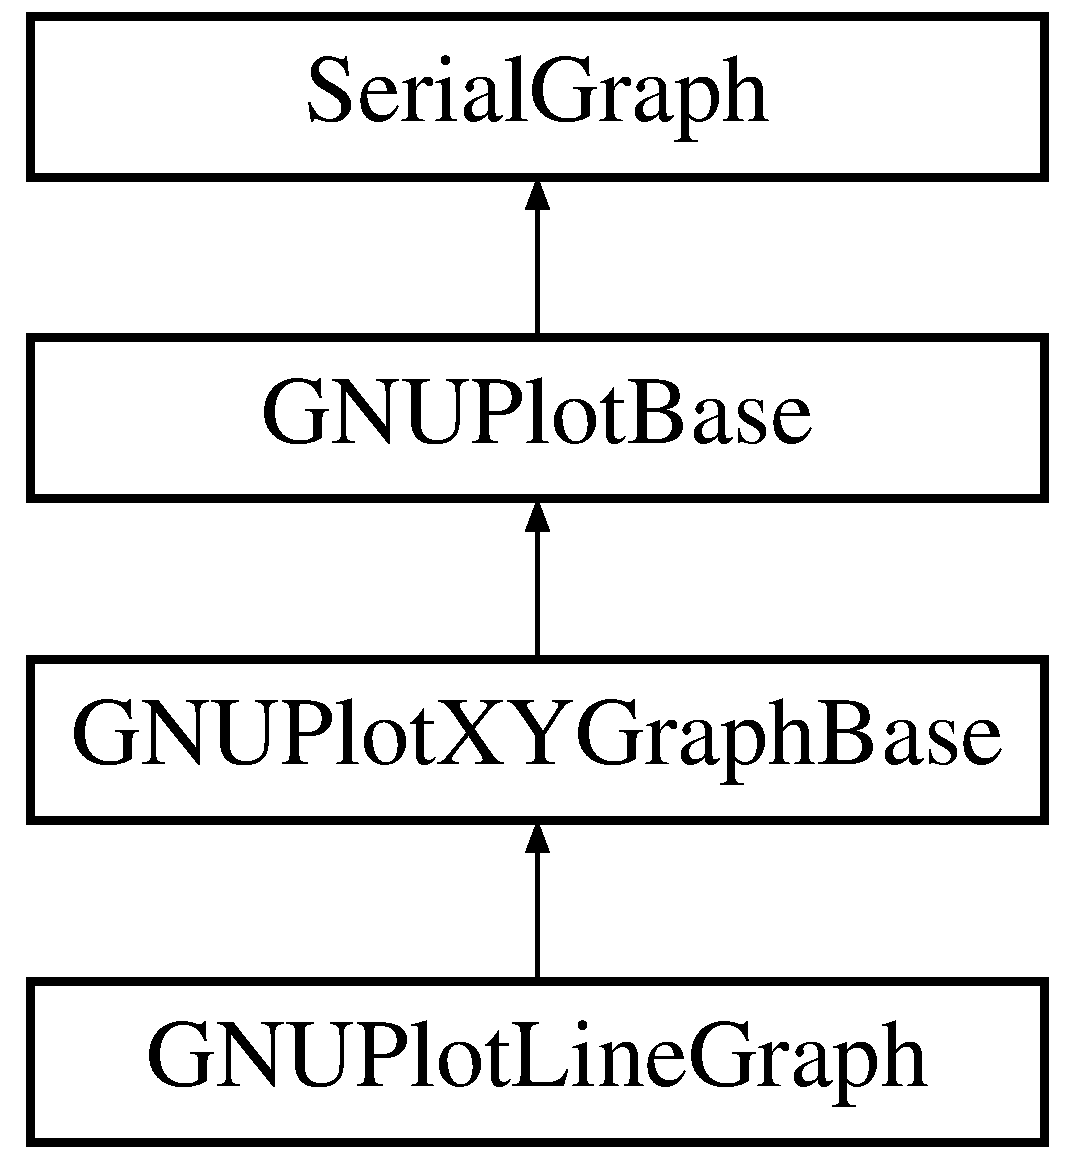
\includegraphics[height=4.000000cm]{class_g_n_u_plot_line_graph}
\end{center}
\end{figure}
\subsection*{Public Member Functions}
\begin{DoxyCompactItemize}
\item 
\hyperlink{class_g_n_u_plot_line_graph_ab014e7473d49843586b58ad89f647801}{G\+N\+U\+Plot\+Line\+Graph} (Print $\ast$\+\_\+out\+Stream)
\item 
virtual \hyperlink{class_g_n_u_plot_line_graph_ae63dcb831b4df37c1d1c877e0d0e671c}{$\sim$\+G\+N\+U\+Plot\+Line\+Graph} ()
\item 
virtual void \hyperlink{class_g_n_u_plot_x_y_graph_base_a8389f830ff330dfb705e00d31053e130}{create\+Graph} ()
\item 
virtual void \hyperlink{class_g_n_u_plot_base_a4d4da234cfdeb99ec3228ef7b2df8a50}{new\+Graph} ()
\item 
virtual void \hyperlink{class_g_n_u_plot_base_aa4b0574c35fbee4dc5f25451eaf956dd}{finish\+Graph} ()
\item 
virtual void \hyperlink{class_g_n_u_plot_base_a219601bd41203477ae73a18d18dd7443}{print\+Comment\+Start} ()
\item 
virtual void \hyperlink{class_serial_graph_a28b020807c52c113685aa6a31f836c52}{enable\+Save\+Image\+File} (bool enabled)
\item 
virtual void \hyperlink{class_serial_graph_abf488e449d6d786bc01478793d0094ad}{set\+Show\+Grid} (bool enabled)
\item 
void \hyperlink{class_serial_graph_a4db09b008589914b71b2ee8b1873db7a}{set\+Title} (const \+\_\+\+\_\+\+Flash\+String\+Helper $\ast$title)
\item 
virtual void \hyperlink{class_serial_graph_ad726b2c84cec50c2d4bfe769e62a9bcd}{set\+Title} (const char $\ast$title)
\item 
void \hyperlink{class_serial_graph_afdb759a860c41de2fc4cfe78519b9fc0}{set\+X\+Axis\+Name} (const \+\_\+\+\_\+\+Flash\+String\+Helper $\ast$title)
\item 
virtual void \hyperlink{class_serial_graph_ac7f30036f5006091af51204a4d9efaf2}{set\+X\+Axis\+Name} (const char $\ast$name)
\item 
void \hyperlink{class_serial_graph_abfc46c15cf8e1b4362a7f51cb11c7bdb}{set\+Y\+Axis\+Name} (const \+\_\+\+\_\+\+Flash\+String\+Helper $\ast$title)
\item 
virtual void \hyperlink{class_serial_graph_ab0c675c8682959261f79dcf37b04148c}{set\+Y\+Axis\+Name} (const char $\ast$name)
\item 
virtual void \hyperlink{class_serial_graph_ae58de4fa4d391f1a2f411ce00dd74d93}{set\+X\+Axis\+Log} (byte scale)
\item 
virtual void \hyperlink{class_serial_graph_a444e38e8ef3784942ca6ee58940f7023}{set\+Y\+Axis\+Log} (byte scale)
\item 
void \hyperlink{class_serial_graph_a84d8e8ce9bff20e53ba738d1d34d3577}{set\+Series\+Name} (int \+\_\+n, const \+\_\+\+\_\+\+Flash\+String\+Helper $\ast$title)
\item 
virtual void \hyperlink{class_serial_graph_a9d67fbecbee6edb82646aa7ba5103046}{set\+Series\+Name} (int \+\_\+n, const char $\ast$name)
\item 
\hyperlink{struct_line_apperance}{Line\+Apperance} $\ast$ \hyperlink{class_serial_graph_a5a6008dc86a2101a58782929721a5b77}{get\+Line\+Apperance} (int \+\_\+n)
\item 
{\footnotesize template$<$typename Y\+T $>$ }\\void \hyperlink{class_serial_graph_afbcc26bd6bad7179d75379ac0f0d25f1}{plot\+Datum\+Y} (Y\+T y1)
\item 
{\footnotesize template$<$typename X\+T , typename Y\+T $>$ }\\void \hyperlink{class_serial_graph_a265b48fb0afe543e14cedb6619e3931e}{plot\+Datum\+X\+Y} (X\+T x, Y\+T y1)
\item 
{\footnotesize template$<$typename Y\+T $>$ }\\void \hyperlink{class_serial_graph_a56f584fa6316175bc9fbcb4f671f1c93}{plot\+Datum\+Yn} (Y\+T y1, Y\+T y2)
\item 
{\footnotesize template$<$typename Y\+T $>$ }\\void \hyperlink{class_serial_graph_ae755b026606e34c33c4aa8f10d8b5d9c}{plot\+Datum\+Yn} (Y\+T y1, Y\+T y2, Y\+T y3)
\item 
{\footnotesize template$<$typename Y\+T $>$ }\\void \hyperlink{class_serial_graph_a354feb95f91239699d3510c2ce5659b0}{plot\+Datum\+Yn} (Y\+T y1, Y\+T y2, Y\+T y3, Y\+T y4)
\item 
{\footnotesize template$<$typename Y\+T $>$ }\\void \hyperlink{class_serial_graph_ab0fff3fc1879e1cd6aadf24c913ff617}{plot\+Datum\+Yn} (Y\+T y1, Y\+T y2, Y\+T y3, Y\+T y4, Y\+T y5)
\item 
{\footnotesize template$<$typename X\+T , typename Y\+T $>$ }\\void \hyperlink{class_serial_graph_aa20b03efac52c18c50efc79c6459a9fc}{plot\+Datum\+Yn} (const Y\+T $\ast$y\+Vec, int \+\_\+n)
\item 
{\footnotesize template$<$typename X\+T , typename Y\+T $>$ }\\void \hyperlink{class_serial_graph_a79b721ca2be68969862869f96d6a6305}{plot\+Datum\+X\+Yn} (X\+T x, Y\+T y1, Y\+T y2)
\item 
{\footnotesize template$<$typename X\+T , typename Y\+T $>$ }\\void \hyperlink{class_serial_graph_a9fcea879f299a7d24be4ff9a38c53c26}{plot\+Datum\+X\+Yn} (X\+T x, Y\+T y1, Y\+T y2, Y\+T y3)
\item 
{\footnotesize template$<$typename X\+T , typename Y\+T $>$ }\\void \hyperlink{class_serial_graph_afd854b631604abe2014a1bb1beeeec52}{plot\+Datum\+X\+Yn} (X\+T x, Y\+T y1, Y\+T y2, Y\+T y3, Y\+T y4)
\item 
{\footnotesize template$<$typename X\+T , typename Y\+T $>$ }\\void \hyperlink{class_serial_graph_aa1bb6fa08a8bd06c074ac2a02b3f6fbc}{plot\+Datum\+X\+Yn} (X\+T x, Y\+T y1, Y\+T y2, Y\+T y3, Y\+T y4, Y\+T y5)
\item 
{\footnotesize template$<$typename X\+T , typename Y\+T $>$ }\\void \hyperlink{class_serial_graph_a3d7276c89235dc1aa176e2439ad9835b}{plot\+Datum\+X\+Yn} (X\+T x, const Y\+T $\ast$y\+Vec, int \+\_\+n)
\item 
{\footnotesize template$<$typename W\+T $>$ }\\void \hyperlink{class_serial_graph_aa72b48968e82a953dcdc6522bd04c7b4}{print} (const W\+T what)
\item 
{\footnotesize template$<$typename W\+T $>$ }\\void \hyperlink{class_serial_graph_a2005d103cb5a578053ef7838b3a8422d}{println} (const W\+T what)
\item 
{\footnotesize template$<$typename W\+T $>$ }\\void \hyperlink{class_serial_graph_a7237d928f67a14d5c9950d8c23c2a794}{print\+Comment} (const W\+T what)
\item 
{\footnotesize template$<$typename W\+T $>$ }\\void \hyperlink{class_serial_graph_a9b40aa22335fc26a6c29b16d278b26f8}{print\+Comment} (const W\+T $\ast$what)
\end{DoxyCompactItemize}
\subsection*{Public Attributes}
\begin{DoxyCompactItemize}
\item 
const byte \hyperlink{class_serial_graph_a1867ab3a93268646490fa7ba4f8b5680}{max\+String\+Size} = 128
\item 
const byte \hyperlink{class_serial_graph_a752a1429bd35687163fe11c5a2562bef}{max\+Series} = 8
\end{DoxyCompactItemize}
\subsection*{Protected Member Functions}
\begin{DoxyCompactItemize}
\item 
virtual \hyperlink{_serial_graph_8h_adc73bce6b7e6c4ecf37dde452d6a385e}{Graph\+Style} \hyperlink{class_g_n_u_plot_line_graph_a8f8b19efd8d8f4f25ccc41635e332593}{get\+Graph\+Style} () const 
\item 
{\footnotesize template$<$typename T , typename U $>$ }\\void \hyperlink{class_g_n_u_plot_base_a03d371b0c6c7ef89064525438b22d52c}{set\+Variable} (T name, U value, bool quoted)
\item 
{\footnotesize template$<$typename T $>$ }\\void \hyperlink{class_g_n_u_plot_base_a3c8c8f68c13661d91bd844589e1a2a85}{set\+Variable} (T name)
\item 
{\footnotesize template$<$typename T $>$ }\\void \hyperlink{class_g_n_u_plot_base_af9b418bbcafb41d4d51b92018ca4f217}{unset\+Variable} (T name)
\item 
{\footnotesize template$<$typename T $>$ }\\void \hyperlink{class_g_n_u_plot_base_a68171bf36461e54e2b81384c112ad975}{set\+Varible\+By\+String\+\_\+null\+Safe} (T name, const char $\ast$text)
\item 
{\footnotesize template$<$typename T $>$ }\\void \hyperlink{class_g_n_u_plot_base_ae93c5de3241c2b6b6f703a202dc1d94b}{set\+Varible\+Flag\+By\+Boolean} (T name, bool value)
\item 
void \hyperlink{class_g_n_u_plot_base_ab5c851953dd140cc3ee936a5cd329200}{save\+Plot\+To\+Image\+File} (const char $\ast$title)
\item 
virtual void \hyperlink{class_g_n_u_plot_base_adaf91c191e4d889537d401faeb863485}{make\+Ready\+For\+Plot\+Data} ()
\item 
char $\ast$ \hyperlink{class_g_n_u_plot_base_a7f71f3c616b3a4a854f9118a04c40447}{malloc\+Basic\+File\+Name\+From\+Graph\+Title} ()
\item 
void \hyperlink{class_g_n_u_plot_base_a65ae2b3220034bce21c7feb39a632991}{print\+Title\+In\+Plot\+Command} (int series\+Num)
\item 
void \hyperlink{class_g_n_u_plot_base_ad057969aa7f8bdbe884d6a5d03a29722}{print\+Line\+Apperance} (\hyperlink{struct_line_apperance}{Line\+Apperance} apperance)
\item 
void \hyperlink{class_g_n_u_plot_base_ad7e8ef8d8e5eb80119fc0cce9be2d525}{print\+Log\+Axis\+Command} (const \+\_\+\+\_\+\+Flash\+String\+Helper $\ast$axis\+Name, byte log\+Scale)
\item 
virtual void \hyperlink{class_g_n_u_plot_base_ae204818b4e8dcd9d2f6b5426127ca2cf}{print\+Seperator} ()
\item 
virtual void \hyperlink{class_g_n_u_plot_base_ac2b48b822b6043392b514c9580b1661a}{print\+Start\+Datum} ()
\item 
virtual void \hyperlink{class_g_n_u_plot_base_aff02bc279e6c3cb83f2cdc7aa021268f}{print\+End\+Datum} ()
\item 
virtual void \hyperlink{class_g_n_u_plot_base_ad00a12fd681e4638fae005891fd72f38}{\+\_\+print\+Data\+Value} (const char $\ast$value)
\item 
virtual void \hyperlink{class_g_n_u_plot_base_aa6c6dfff0568dd99c0c28081c41b4433}{\+\_\+print\+Data\+Value} (char value)
\item 
virtual void \hyperlink{class_g_n_u_plot_base_a6f14fc040ff833c685ab09fc7917e059}{\+\_\+print\+Data\+Value} (bool value)
\item 
virtual void \hyperlink{class_serial_graph_a0c4d2c1239de3107d7332389183b05a1}{\+\_\+print\+Data\+Value} (const \+\_\+\+\_\+\+Flash\+String\+Helper $\ast$value)
\item 
virtual void \hyperlink{class_serial_graph_a58edf4683c600b6bfa1714b0f8dfc82c}{\+\_\+print\+Data\+Value} (int value)
\item 
virtual void \hyperlink{class_serial_graph_a9a4903d4fa26bb85ba5dd93c4365bcc2}{\+\_\+print\+Data\+Value} (long value)
\item 
virtual void \hyperlink{class_serial_graph_acada5333b96b65e31d8c76c3ab22905f}{\+\_\+print\+Data\+Value} (byte value)
\item 
virtual void \hyperlink{class_serial_graph_acd91cf0c3a0f49d4bdf18b447503da23}{\+\_\+print\+Data\+Value} (unsigned int value)
\item 
virtual void \hyperlink{class_serial_graph_a6dbfe61ee398e18c1b752a3748df9663}{\+\_\+print\+Data\+Value} (unsigned long value)
\item 
virtual void \hyperlink{class_serial_graph_a766d5838ede9c8fa998ce8664e5f92be}{\+\_\+print\+Data\+Value} (double value)
\item 
void \hyperlink{class_serial_graph_a760dd00474c9780c81ece7cdf621fc15}{init} ()
\item 
void \hyperlink{class_serial_graph_abd43150abedec26eef3994cd33035173}{ensure\+Ready\+To\+Recive\+Plot\+Data} ()
\item 
{\footnotesize template$<$typename T $>$ }\\void \hyperlink{class_serial_graph_a91e20c05c8cc612fd9ffd85880149264}{print\+Data\+Value} (T value)
\end{DoxyCompactItemize}
\subsection*{Protected Attributes}
\begin{DoxyCompactItemize}
\item 
bool \hyperlink{class_serial_graph_a24202e0a7a8bac5ec1cfd92bf796e078}{save\+File}
\item 
Print $\ast$ \hyperlink{class_serial_graph_aec32289a9393e98bf80d44406e5c207d}{out\+Stream}
\item 
bool \hyperlink{class_serial_graph_a4dbd9cf190c591fb4f2f46a50d937199}{x\+Axis\+Specified}
\item 
int \hyperlink{class_serial_graph_ab40c430e06102b9624736173d4a58596}{num\+Y\+Series}
\item 
bool \hyperlink{class_serial_graph_ad61d5ea29eacc1611c5addc94714f1e2}{show\+Grid}
\item 
char $\ast$ \hyperlink{class_serial_graph_a0b33d43c2bb54340ef1f90b5f76d7aea}{graph\+Title}
\item 
char $\ast$ \hyperlink{class_serial_graph_a5f5bf85ed361ff567d0888eaa73e269c}{x\+Axis\+Name}
\item 
char $\ast$ \hyperlink{class_serial_graph_a08452a56c74ec5f5473b64605d555339}{y\+Axis\+Name}
\item 
char $\ast$$\ast$ \hyperlink{class_serial_graph_a2307e40e27249f44bbe14776dc68c561}{series\+Names}
\item 
\hyperlink{struct_line_apperance}{Line\+Apperance} $\ast$ \hyperlink{class_serial_graph_a8d743f9eeeca69a988d2159a405e4253}{series\+Apperance}
\item 
byte \hyperlink{class_serial_graph_afc2ca72fdfe2bc5e3159c9e910a8f81e}{x\+Axis\+Log\+Scale}
\item 
byte \hyperlink{class_serial_graph_a1f0424857ec14c176747b3ddb0768eee}{y\+Axis\+Log\+Scale}
\end{DoxyCompactItemize}


\subsection{Detailed Description}
Specilisation of \hyperlink{class_g_n_u_plot_x_y_graph_base}{G\+N\+U\+Plot\+X\+Y\+Graph\+Base} to make a nice line plot. \hyperlink{class_g_n_u_plot_line_graph_a8f8b19efd8d8f4f25ccc41635e332593}{G\+N\+U\+Plot\+Line\+Graph\+::get\+Graph\+Style()} alters the behaviour of \hyperlink{class_g_n_u_plot_x_y_graph_base_a8389f830ff330dfb705e00d31053e130}{G\+N\+U\+Plot\+X\+Y\+Graph\+Base\+::create\+Graph()} 

\subsection{Constructor \& Destructor Documentation}
\hypertarget{class_g_n_u_plot_line_graph_ab014e7473d49843586b58ad89f647801}{}\index{G\+N\+U\+Plot\+Line\+Graph@{G\+N\+U\+Plot\+Line\+Graph}!G\+N\+U\+Plot\+Line\+Graph@{G\+N\+U\+Plot\+Line\+Graph}}
\index{G\+N\+U\+Plot\+Line\+Graph@{G\+N\+U\+Plot\+Line\+Graph}!G\+N\+U\+Plot\+Line\+Graph@{G\+N\+U\+Plot\+Line\+Graph}}
\subsubsection[{G\+N\+U\+Plot\+Line\+Graph(\+Print $\ast$\+\_\+out\+Stream)}]{\setlength{\rightskip}{0pt plus 5cm}G\+N\+U\+Plot\+Line\+Graph\+::\+G\+N\+U\+Plot\+Line\+Graph (
\begin{DoxyParamCaption}
\item[{Print $\ast$}]{\+\_\+out\+Stream}
\end{DoxyParamCaption}
)\hspace{0.3cm}{\ttfamily [inline]}}\label{class_g_n_u_plot_line_graph_ab014e7473d49843586b58ad89f647801}
\hypertarget{class_g_n_u_plot_line_graph_ae63dcb831b4df37c1d1c877e0d0e671c}{}\index{G\+N\+U\+Plot\+Line\+Graph@{G\+N\+U\+Plot\+Line\+Graph}!````~G\+N\+U\+Plot\+Line\+Graph@{$\sim$\+G\+N\+U\+Plot\+Line\+Graph}}
\index{````~G\+N\+U\+Plot\+Line\+Graph@{$\sim$\+G\+N\+U\+Plot\+Line\+Graph}!G\+N\+U\+Plot\+Line\+Graph@{G\+N\+U\+Plot\+Line\+Graph}}
\subsubsection[{$\sim$\+G\+N\+U\+Plot\+Line\+Graph()}]{\setlength{\rightskip}{0pt plus 5cm}virtual G\+N\+U\+Plot\+Line\+Graph\+::$\sim$\+G\+N\+U\+Plot\+Line\+Graph (
\begin{DoxyParamCaption}
{}
\end{DoxyParamCaption}
)\hspace{0.3cm}{\ttfamily [inline]}, {\ttfamily [virtual]}}\label{class_g_n_u_plot_line_graph_ae63dcb831b4df37c1d1c877e0d0e671c}


\subsection{Member Function Documentation}
\hypertarget{class_g_n_u_plot_base_ad00a12fd681e4638fae005891fd72f38}{}\index{G\+N\+U\+Plot\+Line\+Graph@{G\+N\+U\+Plot\+Line\+Graph}!\+\_\+print\+Data\+Value@{\+\_\+print\+Data\+Value}}
\index{\+\_\+print\+Data\+Value@{\+\_\+print\+Data\+Value}!G\+N\+U\+Plot\+Line\+Graph@{G\+N\+U\+Plot\+Line\+Graph}}
\subsubsection[{\+\_\+print\+Data\+Value(const char $\ast$value)}]{\setlength{\rightskip}{0pt plus 5cm}void G\+N\+U\+Plot\+Base\+::\+\_\+print\+Data\+Value (
\begin{DoxyParamCaption}
\item[{const char $\ast$}]{value}
\end{DoxyParamCaption}
)\hspace{0.3cm}{\ttfamily [protected]}, {\ttfamily [virtual]}, {\ttfamily [inherited]}}\label{class_g_n_u_plot_base_ad00a12fd681e4638fae005891fd72f38}
Override a put appropriate quotes around strings etc. 
\begin{DoxyParams}{Parameters}
{\em value} & What to print. \\
\hline
\end{DoxyParams}


Reimplemented from \hyperlink{class_serial_graph_a8252997dd4bad0251d437d6dd097bffb}{Serial\+Graph}.

\hypertarget{class_g_n_u_plot_base_aa6c6dfff0568dd99c0c28081c41b4433}{}\index{G\+N\+U\+Plot\+Line\+Graph@{G\+N\+U\+Plot\+Line\+Graph}!\+\_\+print\+Data\+Value@{\+\_\+print\+Data\+Value}}
\index{\+\_\+print\+Data\+Value@{\+\_\+print\+Data\+Value}!G\+N\+U\+Plot\+Line\+Graph@{G\+N\+U\+Plot\+Line\+Graph}}
\subsubsection[{\+\_\+print\+Data\+Value(char value)}]{\setlength{\rightskip}{0pt plus 5cm}virtual void G\+N\+U\+Plot\+Base\+::\+\_\+print\+Data\+Value (
\begin{DoxyParamCaption}
\item[{char}]{value}
\end{DoxyParamCaption}
)\hspace{0.3cm}{\ttfamily [inline]}, {\ttfamily [protected]}, {\ttfamily [virtual]}, {\ttfamily [inherited]}}\label{class_g_n_u_plot_base_aa6c6dfff0568dd99c0c28081c41b4433}
Override for customised value output. 
\begin{DoxyParams}{Parameters}
{\em value} & What to print. \\
\hline
\end{DoxyParams}


Reimplemented from \hyperlink{class_serial_graph_af3fbf7a9201f71cd6bad7e4337092fb6}{Serial\+Graph}.

\hypertarget{class_g_n_u_plot_base_a6f14fc040ff833c685ab09fc7917e059}{}\index{G\+N\+U\+Plot\+Line\+Graph@{G\+N\+U\+Plot\+Line\+Graph}!\+\_\+print\+Data\+Value@{\+\_\+print\+Data\+Value}}
\index{\+\_\+print\+Data\+Value@{\+\_\+print\+Data\+Value}!G\+N\+U\+Plot\+Line\+Graph@{G\+N\+U\+Plot\+Line\+Graph}}
\subsubsection[{\+\_\+print\+Data\+Value(bool value)}]{\setlength{\rightskip}{0pt plus 5cm}virtual void G\+N\+U\+Plot\+Base\+::\+\_\+print\+Data\+Value (
\begin{DoxyParamCaption}
\item[{bool}]{value}
\end{DoxyParamCaption}
)\hspace{0.3cm}{\ttfamily [inline]}, {\ttfamily [protected]}, {\ttfamily [virtual]}, {\ttfamily [inherited]}}\label{class_g_n_u_plot_base_a6f14fc040ff833c685ab09fc7917e059}
Override for customised value output. 
\begin{DoxyParams}{Parameters}
{\em value} & What to print. \\
\hline
\end{DoxyParams}


Reimplemented from \hyperlink{class_serial_graph_aed9ff95634ace3d190863ea9d15c10da}{Serial\+Graph}.

\hypertarget{class_serial_graph_a0c4d2c1239de3107d7332389183b05a1}{}\index{G\+N\+U\+Plot\+Line\+Graph@{G\+N\+U\+Plot\+Line\+Graph}!\+\_\+print\+Data\+Value@{\+\_\+print\+Data\+Value}}
\index{\+\_\+print\+Data\+Value@{\+\_\+print\+Data\+Value}!G\+N\+U\+Plot\+Line\+Graph@{G\+N\+U\+Plot\+Line\+Graph}}
\subsubsection[{\+\_\+print\+Data\+Value(const \+\_\+\+\_\+\+Flash\+String\+Helper $\ast$value)}]{\setlength{\rightskip}{0pt plus 5cm}virtual void Serial\+Graph\+::\+\_\+print\+Data\+Value (
\begin{DoxyParamCaption}
\item[{const \+\_\+\+\_\+\+Flash\+String\+Helper $\ast$}]{value}
\end{DoxyParamCaption}
)\hspace{0.3cm}{\ttfamily [inline]}, {\ttfamily [protected]}, {\ttfamily [virtual]}, {\ttfamily [inherited]}}\label{class_serial_graph_a0c4d2c1239de3107d7332389183b05a1}
This just calls \hyperlink{class_serial_graph_a8252997dd4bad0251d437d6dd097bffb}{\+\_\+print\+Data\+Value(const char $\ast$value)} so probably alter that instead. 
\begin{DoxyParams}{Parameters}
{\em value} & What to print. \\
\hline
\end{DoxyParams}
\hypertarget{class_serial_graph_a58edf4683c600b6bfa1714b0f8dfc82c}{}\index{G\+N\+U\+Plot\+Line\+Graph@{G\+N\+U\+Plot\+Line\+Graph}!\+\_\+print\+Data\+Value@{\+\_\+print\+Data\+Value}}
\index{\+\_\+print\+Data\+Value@{\+\_\+print\+Data\+Value}!G\+N\+U\+Plot\+Line\+Graph@{G\+N\+U\+Plot\+Line\+Graph}}
\subsubsection[{\+\_\+print\+Data\+Value(int value)}]{\setlength{\rightskip}{0pt plus 5cm}virtual void Serial\+Graph\+::\+\_\+print\+Data\+Value (
\begin{DoxyParamCaption}
\item[{int}]{value}
\end{DoxyParamCaption}
)\hspace{0.3cm}{\ttfamily [inline]}, {\ttfamily [protected]}, {\ttfamily [virtual]}, {\ttfamily [inherited]}}\label{class_serial_graph_a58edf4683c600b6bfa1714b0f8dfc82c}
Override for customised value output. 
\begin{DoxyParams}{Parameters}
{\em value} & What to print. \\
\hline
\end{DoxyParams}
\hypertarget{class_serial_graph_a9a4903d4fa26bb85ba5dd93c4365bcc2}{}\index{G\+N\+U\+Plot\+Line\+Graph@{G\+N\+U\+Plot\+Line\+Graph}!\+\_\+print\+Data\+Value@{\+\_\+print\+Data\+Value}}
\index{\+\_\+print\+Data\+Value@{\+\_\+print\+Data\+Value}!G\+N\+U\+Plot\+Line\+Graph@{G\+N\+U\+Plot\+Line\+Graph}}
\subsubsection[{\+\_\+print\+Data\+Value(long value)}]{\setlength{\rightskip}{0pt plus 5cm}virtual void Serial\+Graph\+::\+\_\+print\+Data\+Value (
\begin{DoxyParamCaption}
\item[{long}]{value}
\end{DoxyParamCaption}
)\hspace{0.3cm}{\ttfamily [inline]}, {\ttfamily [protected]}, {\ttfamily [virtual]}, {\ttfamily [inherited]}}\label{class_serial_graph_a9a4903d4fa26bb85ba5dd93c4365bcc2}
Override for customised value output. 
\begin{DoxyParams}{Parameters}
{\em value} & What to print. \\
\hline
\end{DoxyParams}
\hypertarget{class_serial_graph_acada5333b96b65e31d8c76c3ab22905f}{}\index{G\+N\+U\+Plot\+Line\+Graph@{G\+N\+U\+Plot\+Line\+Graph}!\+\_\+print\+Data\+Value@{\+\_\+print\+Data\+Value}}
\index{\+\_\+print\+Data\+Value@{\+\_\+print\+Data\+Value}!G\+N\+U\+Plot\+Line\+Graph@{G\+N\+U\+Plot\+Line\+Graph}}
\subsubsection[{\+\_\+print\+Data\+Value(byte value)}]{\setlength{\rightskip}{0pt plus 5cm}virtual void Serial\+Graph\+::\+\_\+print\+Data\+Value (
\begin{DoxyParamCaption}
\item[{byte}]{value}
\end{DoxyParamCaption}
)\hspace{0.3cm}{\ttfamily [inline]}, {\ttfamily [protected]}, {\ttfamily [virtual]}, {\ttfamily [inherited]}}\label{class_serial_graph_acada5333b96b65e31d8c76c3ab22905f}
Override for customised value output. 
\begin{DoxyParams}{Parameters}
{\em value} & What to print. \\
\hline
\end{DoxyParams}
\hypertarget{class_serial_graph_acd91cf0c3a0f49d4bdf18b447503da23}{}\index{G\+N\+U\+Plot\+Line\+Graph@{G\+N\+U\+Plot\+Line\+Graph}!\+\_\+print\+Data\+Value@{\+\_\+print\+Data\+Value}}
\index{\+\_\+print\+Data\+Value@{\+\_\+print\+Data\+Value}!G\+N\+U\+Plot\+Line\+Graph@{G\+N\+U\+Plot\+Line\+Graph}}
\subsubsection[{\+\_\+print\+Data\+Value(unsigned int value)}]{\setlength{\rightskip}{0pt plus 5cm}virtual void Serial\+Graph\+::\+\_\+print\+Data\+Value (
\begin{DoxyParamCaption}
\item[{unsigned int}]{value}
\end{DoxyParamCaption}
)\hspace{0.3cm}{\ttfamily [inline]}, {\ttfamily [protected]}, {\ttfamily [virtual]}, {\ttfamily [inherited]}}\label{class_serial_graph_acd91cf0c3a0f49d4bdf18b447503da23}
Override for customised value output. 
\begin{DoxyParams}{Parameters}
{\em value} & What to print. \\
\hline
\end{DoxyParams}
\hypertarget{class_serial_graph_a6dbfe61ee398e18c1b752a3748df9663}{}\index{G\+N\+U\+Plot\+Line\+Graph@{G\+N\+U\+Plot\+Line\+Graph}!\+\_\+print\+Data\+Value@{\+\_\+print\+Data\+Value}}
\index{\+\_\+print\+Data\+Value@{\+\_\+print\+Data\+Value}!G\+N\+U\+Plot\+Line\+Graph@{G\+N\+U\+Plot\+Line\+Graph}}
\subsubsection[{\+\_\+print\+Data\+Value(unsigned long value)}]{\setlength{\rightskip}{0pt plus 5cm}virtual void Serial\+Graph\+::\+\_\+print\+Data\+Value (
\begin{DoxyParamCaption}
\item[{unsigned long}]{value}
\end{DoxyParamCaption}
)\hspace{0.3cm}{\ttfamily [inline]}, {\ttfamily [protected]}, {\ttfamily [virtual]}, {\ttfamily [inherited]}}\label{class_serial_graph_a6dbfe61ee398e18c1b752a3748df9663}
Override for customised value output. 
\begin{DoxyParams}{Parameters}
{\em value} & What to print. \\
\hline
\end{DoxyParams}
\hypertarget{class_serial_graph_a766d5838ede9c8fa998ce8664e5f92be}{}\index{G\+N\+U\+Plot\+Line\+Graph@{G\+N\+U\+Plot\+Line\+Graph}!\+\_\+print\+Data\+Value@{\+\_\+print\+Data\+Value}}
\index{\+\_\+print\+Data\+Value@{\+\_\+print\+Data\+Value}!G\+N\+U\+Plot\+Line\+Graph@{G\+N\+U\+Plot\+Line\+Graph}}
\subsubsection[{\+\_\+print\+Data\+Value(double value)}]{\setlength{\rightskip}{0pt plus 5cm}virtual void Serial\+Graph\+::\+\_\+print\+Data\+Value (
\begin{DoxyParamCaption}
\item[{double}]{value}
\end{DoxyParamCaption}
)\hspace{0.3cm}{\ttfamily [inline]}, {\ttfamily [protected]}, {\ttfamily [virtual]}, {\ttfamily [inherited]}}\label{class_serial_graph_a766d5838ede9c8fa998ce8664e5f92be}
Override for customised value output. 
\begin{DoxyParams}{Parameters}
{\em value} & What to print. \\
\hline
\end{DoxyParams}
\hypertarget{class_g_n_u_plot_x_y_graph_base_a8389f830ff330dfb705e00d31053e130}{}\index{G\+N\+U\+Plot\+Line\+Graph@{G\+N\+U\+Plot\+Line\+Graph}!create\+Graph@{create\+Graph}}
\index{create\+Graph@{create\+Graph}!G\+N\+U\+Plot\+Line\+Graph@{G\+N\+U\+Plot\+Line\+Graph}}
\subsubsection[{create\+Graph()}]{\setlength{\rightskip}{0pt plus 5cm}void G\+N\+U\+Plot\+X\+Y\+Graph\+Base\+::create\+Graph (
\begin{DoxyParamCaption}
{}
\end{DoxyParamCaption}
)\hspace{0.3cm}{\ttfamily [virtual]}, {\ttfamily [inherited]}}\label{class_g_n_u_plot_x_y_graph_base_a8389f830ff330dfb705e00d31053e130}


Implements \hyperlink{class_g_n_u_plot_base_ad877f207d43e6f9cd0aa0ef241e31c24}{G\+N\+U\+Plot\+Base}.

\hypertarget{class_serial_graph_a28b020807c52c113685aa6a31f836c52}{}\index{G\+N\+U\+Plot\+Line\+Graph@{G\+N\+U\+Plot\+Line\+Graph}!enable\+Save\+Image\+File@{enable\+Save\+Image\+File}}
\index{enable\+Save\+Image\+File@{enable\+Save\+Image\+File}!G\+N\+U\+Plot\+Line\+Graph@{G\+N\+U\+Plot\+Line\+Graph}}
\subsubsection[{enable\+Save\+Image\+File(bool enabled)}]{\setlength{\rightskip}{0pt plus 5cm}virtual void Serial\+Graph\+::enable\+Save\+Image\+File (
\begin{DoxyParamCaption}
\item[{bool}]{enabled}
\end{DoxyParamCaption}
)\hspace{0.3cm}{\ttfamily [inline]}, {\ttfamily [virtual]}, {\ttfamily [inherited]}}\label{class_serial_graph_a28b020807c52c113685aa6a31f836c52}
Set to true if an image file should be saved. \begin{DoxyNote}{Note}
Filename will be based on graph title. This is done to save memory. Final filename has some extra validation performed to conform with filename rules aplicable to modern operating systems (excluding 8 char limit). 
\end{DoxyNote}
\hypertarget{class_serial_graph_abd43150abedec26eef3994cd33035173}{}\index{G\+N\+U\+Plot\+Line\+Graph@{G\+N\+U\+Plot\+Line\+Graph}!ensure\+Ready\+To\+Recive\+Plot\+Data@{ensure\+Ready\+To\+Recive\+Plot\+Data}}
\index{ensure\+Ready\+To\+Recive\+Plot\+Data@{ensure\+Ready\+To\+Recive\+Plot\+Data}!G\+N\+U\+Plot\+Line\+Graph@{G\+N\+U\+Plot\+Line\+Graph}}
\subsubsection[{ensure\+Ready\+To\+Recive\+Plot\+Data()}]{\setlength{\rightskip}{0pt plus 5cm}void Serial\+Graph\+::ensure\+Ready\+To\+Recive\+Plot\+Data (
\begin{DoxyParamCaption}
{}
\end{DoxyParamCaption}
)\hspace{0.3cm}{\ttfamily [protected]}, {\ttfamily [inherited]}}\label{class_serial_graph_abd43150abedec26eef3994cd33035173}
Called by every plot command prior to sending data. it\textquotesingle{}s function is to call \hyperlink{class_serial_graph_a898cf274c886e0ff45e90d3f21f0a6cc}{make\+Ready\+For\+Plot\+Data()} the first time it is called. 
\begin{DoxyParams}{Parameters}
{\em value} & What to print. \\
\hline
\end{DoxyParams}
\hypertarget{class_g_n_u_plot_base_aa4b0574c35fbee4dc5f25451eaf956dd}{}\index{G\+N\+U\+Plot\+Line\+Graph@{G\+N\+U\+Plot\+Line\+Graph}!finish\+Graph@{finish\+Graph}}
\index{finish\+Graph@{finish\+Graph}!G\+N\+U\+Plot\+Line\+Graph@{G\+N\+U\+Plot\+Line\+Graph}}
\subsubsection[{finish\+Graph()}]{\setlength{\rightskip}{0pt plus 5cm}void G\+N\+U\+Plot\+Base\+::finish\+Graph (
\begin{DoxyParamCaption}
{}
\end{DoxyParamCaption}
)\hspace{0.3cm}{\ttfamily [virtual]}, {\ttfamily [inherited]}}\label{class_g_n_u_plot_base_aa4b0574c35fbee4dc5f25451eaf956dd}
Serial output that finishes the plot, saves file, updates display etc. 

Implements \hyperlink{class_serial_graph_a8054ce989a1788bd35d2fde56081c88c}{Serial\+Graph}.

\hypertarget{class_g_n_u_plot_line_graph_a8f8b19efd8d8f4f25ccc41635e332593}{}\index{G\+N\+U\+Plot\+Line\+Graph@{G\+N\+U\+Plot\+Line\+Graph}!get\+Graph\+Style@{get\+Graph\+Style}}
\index{get\+Graph\+Style@{get\+Graph\+Style}!G\+N\+U\+Plot\+Line\+Graph@{G\+N\+U\+Plot\+Line\+Graph}}
\subsubsection[{get\+Graph\+Style() const }]{\setlength{\rightskip}{0pt plus 5cm}virtual {\bf Graph\+Style} G\+N\+U\+Plot\+Line\+Graph\+::get\+Graph\+Style (
\begin{DoxyParamCaption}
{}
\end{DoxyParamCaption}
) const\hspace{0.3cm}{\ttfamily [inline]}, {\ttfamily [protected]}, {\ttfamily [virtual]}}\label{class_g_n_u_plot_line_graph_a8f8b19efd8d8f4f25ccc41635e332593}
Returns the Graph\+Style of the current object. 

Implements \hyperlink{class_serial_graph_a2ab97096fffdf429bfa271b9fd4c642a}{Serial\+Graph}.

\hypertarget{class_serial_graph_a5a6008dc86a2101a58782929721a5b77}{}\index{G\+N\+U\+Plot\+Line\+Graph@{G\+N\+U\+Plot\+Line\+Graph}!get\+Line\+Apperance@{get\+Line\+Apperance}}
\index{get\+Line\+Apperance@{get\+Line\+Apperance}!G\+N\+U\+Plot\+Line\+Graph@{G\+N\+U\+Plot\+Line\+Graph}}
\subsubsection[{get\+Line\+Apperance(int \+\_\+n)}]{\setlength{\rightskip}{0pt plus 5cm}{\bf Line\+Apperance}$\ast$ Serial\+Graph\+::get\+Line\+Apperance (
\begin{DoxyParamCaption}
\item[{int}]{\+\_\+n}
\end{DoxyParamCaption}
)\hspace{0.3cm}{\ttfamily [inline]}, {\ttfamily [inherited]}}\label{class_serial_graph_a5a6008dc86a2101a58782929721a5b77}
Gets a structure that controls apperance of a series (called a \hyperlink{struct_line_apperance}{Line\+Apperance}). It is intended that you directly modify the structure returned, there is no set\+Line\+Apperance. See the struct \hyperlink{struct_line_apperance}{Line\+Apperance} for more.


\begin{DoxyParams}{Parameters}
{\em \+\_\+n} & Series number to alter.\\
\hline
\end{DoxyParams}
\begin{DoxyNote}{Note}
Behaviour on \+\_\+n $>$ max\+Series, is to just override the last possible series entry. 
\end{DoxyNote}
\hypertarget{class_serial_graph_a760dd00474c9780c81ece7cdf621fc15}{}\index{G\+N\+U\+Plot\+Line\+Graph@{G\+N\+U\+Plot\+Line\+Graph}!init@{init}}
\index{init@{init}!G\+N\+U\+Plot\+Line\+Graph@{G\+N\+U\+Plot\+Line\+Graph}}
\subsubsection[{init()}]{\setlength{\rightskip}{0pt plus 5cm}void Serial\+Graph\+::init (
\begin{DoxyParamCaption}
{}
\end{DoxyParamCaption}
)\hspace{0.3cm}{\ttfamily [protected]}, {\ttfamily [inherited]}}\label{class_serial_graph_a760dd00474c9780c81ece7cdf621fc15}
Brings the class to its default state. Called by the constructor and \hyperlink{class_serial_graph_a44d34593c56aa67142ccd9fcc0a1da86}{new\+Graph()}. \hypertarget{class_g_n_u_plot_base_adaf91c191e4d889537d401faeb863485}{}\index{G\+N\+U\+Plot\+Line\+Graph@{G\+N\+U\+Plot\+Line\+Graph}!make\+Ready\+For\+Plot\+Data@{make\+Ready\+For\+Plot\+Data}}
\index{make\+Ready\+For\+Plot\+Data@{make\+Ready\+For\+Plot\+Data}!G\+N\+U\+Plot\+Line\+Graph@{G\+N\+U\+Plot\+Line\+Graph}}
\subsubsection[{make\+Ready\+For\+Plot\+Data()}]{\setlength{\rightskip}{0pt plus 5cm}void G\+N\+U\+Plot\+Base\+::make\+Ready\+For\+Plot\+Data (
\begin{DoxyParamCaption}
{}
\end{DoxyParamCaption}
)\hspace{0.3cm}{\ttfamily [protected]}, {\ttfamily [virtual]}, {\ttfamily [inherited]}}\label{class_g_n_u_plot_base_adaf91c191e4d889537d401faeb863485}
Called by ensure\+Ready\+To\+Recive\+Plot\+Data, if the first plot command is encountered. \begin{DoxyNote}{Note}
A concrete class should override this. 
\end{DoxyNote}


Reimplemented from \hyperlink{class_serial_graph_a898cf274c886e0ff45e90d3f21f0a6cc}{Serial\+Graph}.

\hypertarget{class_g_n_u_plot_base_a7f71f3c616b3a4a854f9118a04c40447}{}\index{G\+N\+U\+Plot\+Line\+Graph@{G\+N\+U\+Plot\+Line\+Graph}!malloc\+Basic\+File\+Name\+From\+Graph\+Title@{malloc\+Basic\+File\+Name\+From\+Graph\+Title}}
\index{malloc\+Basic\+File\+Name\+From\+Graph\+Title@{malloc\+Basic\+File\+Name\+From\+Graph\+Title}!G\+N\+U\+Plot\+Line\+Graph@{G\+N\+U\+Plot\+Line\+Graph}}
\subsubsection[{malloc\+Basic\+File\+Name\+From\+Graph\+Title()}]{\setlength{\rightskip}{0pt plus 5cm}char $\ast$ G\+N\+U\+Plot\+Base\+::malloc\+Basic\+File\+Name\+From\+Graph\+Title (
\begin{DoxyParamCaption}
{}
\end{DoxyParamCaption}
)\hspace{0.3cm}{\ttfamily [protected]}, {\ttfamily [inherited]}}\label{class_g_n_u_plot_base_a7f71f3c616b3a4a854f9118a04c40447}
\hypertarget{class_g_n_u_plot_base_a4d4da234cfdeb99ec3228ef7b2df8a50}{}\index{G\+N\+U\+Plot\+Line\+Graph@{G\+N\+U\+Plot\+Line\+Graph}!new\+Graph@{new\+Graph}}
\index{new\+Graph@{new\+Graph}!G\+N\+U\+Plot\+Line\+Graph@{G\+N\+U\+Plot\+Line\+Graph}}
\subsubsection[{new\+Graph()}]{\setlength{\rightskip}{0pt plus 5cm}void G\+N\+U\+Plot\+Base\+::new\+Graph (
\begin{DoxyParamCaption}
{}
\end{DoxyParamCaption}
)\hspace{0.3cm}{\ttfamily [virtual]}, {\ttfamily [inherited]}}\label{class_g_n_u_plot_base_a4d4da234cfdeb99ec3228ef7b2df8a50}
Serial output that establishes a new graph. This should also call \hyperlink{class_serial_graph_a760dd00474c9780c81ece7cdf621fc15}{init()}, to reset the class. \begin{DoxyNote}{Note}
\+: If you wan\textquotesingle{}t a \char`\"{}memory breather\char`\"{} between plots, calling this method frees all series names, titles etc. 
\end{DoxyNote}


Implements \hyperlink{class_serial_graph_a44d34593c56aa67142ccd9fcc0a1da86}{Serial\+Graph}.

\hypertarget{class_serial_graph_a265b48fb0afe543e14cedb6619e3931e}{}\index{G\+N\+U\+Plot\+Line\+Graph@{G\+N\+U\+Plot\+Line\+Graph}!plot\+Datum\+X\+Y@{plot\+Datum\+X\+Y}}
\index{plot\+Datum\+X\+Y@{plot\+Datum\+X\+Y}!G\+N\+U\+Plot\+Line\+Graph@{G\+N\+U\+Plot\+Line\+Graph}}
\subsubsection[{plot\+Datum\+X\+Y(\+X\+T x, Y\+T y1)}]{\setlength{\rightskip}{0pt plus 5cm}template$<$typename X\+T , typename Y\+T $>$ void Serial\+Graph\+::plot\+Datum\+X\+Y (
\begin{DoxyParamCaption}
\item[{X\+T}]{x, }
\item[{Y\+T}]{y1}
\end{DoxyParamCaption}
)\hspace{0.3cm}{\ttfamily [inline]}, {\ttfamily [inherited]}}\label{class_serial_graph_a265b48fb0afe543e14cedb6619e3931e}
Outputs a point to be plotted. All Y values must be of the same type.

\begin{DoxyNote}{Note}
The first time this is called after \hyperlink{class_serial_graph_a44d34593c56aa67142ccd9fcc0a1da86}{new\+Graph()}, \hyperlink{class_serial_graph_a898cf274c886e0ff45e90d3f21f0a6cc}{make\+Ready\+For\+Plot\+Data()} will be called. 

The following feilds automatically set\+: x\+Axis\+Specified; num\+Y\+Series; 
\end{DoxyNote}
\hypertarget{class_serial_graph_a79b721ca2be68969862869f96d6a6305}{}\index{G\+N\+U\+Plot\+Line\+Graph@{G\+N\+U\+Plot\+Line\+Graph}!plot\+Datum\+X\+Yn@{plot\+Datum\+X\+Yn}}
\index{plot\+Datum\+X\+Yn@{plot\+Datum\+X\+Yn}!G\+N\+U\+Plot\+Line\+Graph@{G\+N\+U\+Plot\+Line\+Graph}}
\subsubsection[{plot\+Datum\+X\+Yn(\+X\+T x, Y\+T y1, Y\+T y2)}]{\setlength{\rightskip}{0pt plus 5cm}template$<$typename X\+T , typename Y\+T $>$ void Serial\+Graph\+::plot\+Datum\+X\+Yn (
\begin{DoxyParamCaption}
\item[{X\+T}]{x, }
\item[{Y\+T}]{y1, }
\item[{Y\+T}]{y2}
\end{DoxyParamCaption}
)\hspace{0.3cm}{\ttfamily [inline]}, {\ttfamily [inherited]}}\label{class_serial_graph_a79b721ca2be68969862869f96d6a6305}
Outputs a point to be plotted. All Y values must be of the same type.

\begin{DoxyNote}{Note}
The first time this is called after \hyperlink{class_serial_graph_a44d34593c56aa67142ccd9fcc0a1da86}{new\+Graph()}, \hyperlink{class_serial_graph_a898cf274c886e0ff45e90d3f21f0a6cc}{make\+Ready\+For\+Plot\+Data()} will be called. 

The following feilds automatically set\+: x\+Axis\+Specified; num\+Y\+Series; 
\end{DoxyNote}
\hypertarget{class_serial_graph_a9fcea879f299a7d24be4ff9a38c53c26}{}\index{G\+N\+U\+Plot\+Line\+Graph@{G\+N\+U\+Plot\+Line\+Graph}!plot\+Datum\+X\+Yn@{plot\+Datum\+X\+Yn}}
\index{plot\+Datum\+X\+Yn@{plot\+Datum\+X\+Yn}!G\+N\+U\+Plot\+Line\+Graph@{G\+N\+U\+Plot\+Line\+Graph}}
\subsubsection[{plot\+Datum\+X\+Yn(\+X\+T x, Y\+T y1, Y\+T y2, Y\+T y3)}]{\setlength{\rightskip}{0pt plus 5cm}template$<$typename X\+T , typename Y\+T $>$ void Serial\+Graph\+::plot\+Datum\+X\+Yn (
\begin{DoxyParamCaption}
\item[{X\+T}]{x, }
\item[{Y\+T}]{y1, }
\item[{Y\+T}]{y2, }
\item[{Y\+T}]{y3}
\end{DoxyParamCaption}
)\hspace{0.3cm}{\ttfamily [inline]}, {\ttfamily [inherited]}}\label{class_serial_graph_a9fcea879f299a7d24be4ff9a38c53c26}
Outputs a point to be plotted. All Y values must be of the same type.

\begin{DoxyNote}{Note}
The first time this is called after \hyperlink{class_serial_graph_a44d34593c56aa67142ccd9fcc0a1da86}{new\+Graph()}, \hyperlink{class_serial_graph_a898cf274c886e0ff45e90d3f21f0a6cc}{make\+Ready\+For\+Plot\+Data()} will be called. 

The following feilds automatically set\+: x\+Axis\+Specified; num\+Y\+Series; 
\end{DoxyNote}
\hypertarget{class_serial_graph_afd854b631604abe2014a1bb1beeeec52}{}\index{G\+N\+U\+Plot\+Line\+Graph@{G\+N\+U\+Plot\+Line\+Graph}!plot\+Datum\+X\+Yn@{plot\+Datum\+X\+Yn}}
\index{plot\+Datum\+X\+Yn@{plot\+Datum\+X\+Yn}!G\+N\+U\+Plot\+Line\+Graph@{G\+N\+U\+Plot\+Line\+Graph}}
\subsubsection[{plot\+Datum\+X\+Yn(\+X\+T x, Y\+T y1, Y\+T y2, Y\+T y3, Y\+T y4)}]{\setlength{\rightskip}{0pt plus 5cm}template$<$typename X\+T , typename Y\+T $>$ void Serial\+Graph\+::plot\+Datum\+X\+Yn (
\begin{DoxyParamCaption}
\item[{X\+T}]{x, }
\item[{Y\+T}]{y1, }
\item[{Y\+T}]{y2, }
\item[{Y\+T}]{y3, }
\item[{Y\+T}]{y4}
\end{DoxyParamCaption}
)\hspace{0.3cm}{\ttfamily [inline]}, {\ttfamily [inherited]}}\label{class_serial_graph_afd854b631604abe2014a1bb1beeeec52}
Outputs a point to be plotted. All Y values must be of the same type.

\begin{DoxyNote}{Note}
The first time this is called after \hyperlink{class_serial_graph_a44d34593c56aa67142ccd9fcc0a1da86}{new\+Graph()}, \hyperlink{class_serial_graph_a898cf274c886e0ff45e90d3f21f0a6cc}{make\+Ready\+For\+Plot\+Data()} will be called. 

The following feilds automatically set\+: x\+Axis\+Specified; num\+Y\+Series; 
\end{DoxyNote}
\hypertarget{class_serial_graph_aa1bb6fa08a8bd06c074ac2a02b3f6fbc}{}\index{G\+N\+U\+Plot\+Line\+Graph@{G\+N\+U\+Plot\+Line\+Graph}!plot\+Datum\+X\+Yn@{plot\+Datum\+X\+Yn}}
\index{plot\+Datum\+X\+Yn@{plot\+Datum\+X\+Yn}!G\+N\+U\+Plot\+Line\+Graph@{G\+N\+U\+Plot\+Line\+Graph}}
\subsubsection[{plot\+Datum\+X\+Yn(\+X\+T x, Y\+T y1, Y\+T y2, Y\+T y3, Y\+T y4, Y\+T y5)}]{\setlength{\rightskip}{0pt plus 5cm}template$<$typename X\+T , typename Y\+T $>$ void Serial\+Graph\+::plot\+Datum\+X\+Yn (
\begin{DoxyParamCaption}
\item[{X\+T}]{x, }
\item[{Y\+T}]{y1, }
\item[{Y\+T}]{y2, }
\item[{Y\+T}]{y3, }
\item[{Y\+T}]{y4, }
\item[{Y\+T}]{y5}
\end{DoxyParamCaption}
)\hspace{0.3cm}{\ttfamily [inline]}, {\ttfamily [inherited]}}\label{class_serial_graph_aa1bb6fa08a8bd06c074ac2a02b3f6fbc}
Outputs a point to be plotted. All Y values must be of the same type.

\begin{DoxyNote}{Note}
The first time this is called after \hyperlink{class_serial_graph_a44d34593c56aa67142ccd9fcc0a1da86}{new\+Graph()}, \hyperlink{class_serial_graph_a898cf274c886e0ff45e90d3f21f0a6cc}{make\+Ready\+For\+Plot\+Data()} will be called. 

The following feilds automatically set\+: x\+Axis\+Specified; num\+Y\+Series; 
\end{DoxyNote}
\hypertarget{class_serial_graph_a3d7276c89235dc1aa176e2439ad9835b}{}\index{G\+N\+U\+Plot\+Line\+Graph@{G\+N\+U\+Plot\+Line\+Graph}!plot\+Datum\+X\+Yn@{plot\+Datum\+X\+Yn}}
\index{plot\+Datum\+X\+Yn@{plot\+Datum\+X\+Yn}!G\+N\+U\+Plot\+Line\+Graph@{G\+N\+U\+Plot\+Line\+Graph}}
\subsubsection[{plot\+Datum\+X\+Yn(\+X\+T x, const Y\+T $\ast$y\+Vec, int \+\_\+n)}]{\setlength{\rightskip}{0pt plus 5cm}template$<$typename X\+T , typename Y\+T $>$ void Serial\+Graph\+::plot\+Datum\+X\+Yn (
\begin{DoxyParamCaption}
\item[{X\+T}]{x, }
\item[{const Y\+T $\ast$}]{y\+Vec, }
\item[{int}]{\+\_\+n}
\end{DoxyParamCaption}
)\hspace{0.3cm}{\ttfamily [inline]}, {\ttfamily [inherited]}}\label{class_serial_graph_a3d7276c89235dc1aa176e2439ad9835b}
Outputs a point to be plotted. All Y values must be of the same type.


\begin{DoxyParams}{Parameters}
{\em y\+Vec} & Pointer to an array of y\+Values. \\
\hline
{\em \+\_\+n} & Number of items in array.\\
\hline
\end{DoxyParams}
\begin{DoxyNote}{Note}
Behaviour on \+\_\+n $>$ max\+Series, is to just override the last possible series entry. 
\end{DoxyNote}
\hypertarget{class_serial_graph_afbcc26bd6bad7179d75379ac0f0d25f1}{}\index{G\+N\+U\+Plot\+Line\+Graph@{G\+N\+U\+Plot\+Line\+Graph}!plot\+Datum\+Y@{plot\+Datum\+Y}}
\index{plot\+Datum\+Y@{plot\+Datum\+Y}!G\+N\+U\+Plot\+Line\+Graph@{G\+N\+U\+Plot\+Line\+Graph}}
\subsubsection[{plot\+Datum\+Y(\+Y\+T y1)}]{\setlength{\rightskip}{0pt plus 5cm}template$<$typename Y\+T $>$ void Serial\+Graph\+::plot\+Datum\+Y (
\begin{DoxyParamCaption}
\item[{Y\+T}]{y1}
\end{DoxyParamCaption}
)\hspace{0.3cm}{\ttfamily [inline]}, {\ttfamily [inherited]}}\label{class_serial_graph_afbcc26bd6bad7179d75379ac0f0d25f1}
Outputs a point to be plotted. All Y values must be of the same type.

\begin{DoxyNote}{Note}
The first time this is called after \hyperlink{class_serial_graph_a44d34593c56aa67142ccd9fcc0a1da86}{new\+Graph()}, \hyperlink{class_serial_graph_a898cf274c886e0ff45e90d3f21f0a6cc}{make\+Ready\+For\+Plot\+Data()} will be called. 

The following feilds automatically set\+: x\+Axis\+Specified; num\+Y\+Series; 
\end{DoxyNote}
\hypertarget{class_serial_graph_a56f584fa6316175bc9fbcb4f671f1c93}{}\index{G\+N\+U\+Plot\+Line\+Graph@{G\+N\+U\+Plot\+Line\+Graph}!plot\+Datum\+Yn@{plot\+Datum\+Yn}}
\index{plot\+Datum\+Yn@{plot\+Datum\+Yn}!G\+N\+U\+Plot\+Line\+Graph@{G\+N\+U\+Plot\+Line\+Graph}}
\subsubsection[{plot\+Datum\+Yn(\+Y\+T y1, Y\+T y2)}]{\setlength{\rightskip}{0pt plus 5cm}template$<$typename Y\+T $>$ void Serial\+Graph\+::plot\+Datum\+Yn (
\begin{DoxyParamCaption}
\item[{Y\+T}]{y1, }
\item[{Y\+T}]{y2}
\end{DoxyParamCaption}
)\hspace{0.3cm}{\ttfamily [inline]}, {\ttfamily [inherited]}}\label{class_serial_graph_a56f584fa6316175bc9fbcb4f671f1c93}
Outputs a point to be plotted. All Y values must be of the same type.

\begin{DoxyNote}{Note}
The first time this is called after \hyperlink{class_serial_graph_a44d34593c56aa67142ccd9fcc0a1da86}{new\+Graph()}, \hyperlink{class_serial_graph_a898cf274c886e0ff45e90d3f21f0a6cc}{make\+Ready\+For\+Plot\+Data()} will be called. 

The following feilds automatically set\+: x\+Axis\+Specified; num\+Y\+Series; 
\end{DoxyNote}
\hypertarget{class_serial_graph_ae755b026606e34c33c4aa8f10d8b5d9c}{}\index{G\+N\+U\+Plot\+Line\+Graph@{G\+N\+U\+Plot\+Line\+Graph}!plot\+Datum\+Yn@{plot\+Datum\+Yn}}
\index{plot\+Datum\+Yn@{plot\+Datum\+Yn}!G\+N\+U\+Plot\+Line\+Graph@{G\+N\+U\+Plot\+Line\+Graph}}
\subsubsection[{plot\+Datum\+Yn(\+Y\+T y1, Y\+T y2, Y\+T y3)}]{\setlength{\rightskip}{0pt plus 5cm}template$<$typename Y\+T $>$ void Serial\+Graph\+::plot\+Datum\+Yn (
\begin{DoxyParamCaption}
\item[{Y\+T}]{y1, }
\item[{Y\+T}]{y2, }
\item[{Y\+T}]{y3}
\end{DoxyParamCaption}
)\hspace{0.3cm}{\ttfamily [inline]}, {\ttfamily [inherited]}}\label{class_serial_graph_ae755b026606e34c33c4aa8f10d8b5d9c}
Outputs a point to be plotted. All Y values must be of the same type.

\begin{DoxyNote}{Note}
The first time this is called after \hyperlink{class_serial_graph_a44d34593c56aa67142ccd9fcc0a1da86}{new\+Graph()}, \hyperlink{class_serial_graph_a898cf274c886e0ff45e90d3f21f0a6cc}{make\+Ready\+For\+Plot\+Data()} will be called. 

The following feilds automatically set\+: x\+Axis\+Specified; num\+Y\+Series; 
\end{DoxyNote}
\hypertarget{class_serial_graph_a354feb95f91239699d3510c2ce5659b0}{}\index{G\+N\+U\+Plot\+Line\+Graph@{G\+N\+U\+Plot\+Line\+Graph}!plot\+Datum\+Yn@{plot\+Datum\+Yn}}
\index{plot\+Datum\+Yn@{plot\+Datum\+Yn}!G\+N\+U\+Plot\+Line\+Graph@{G\+N\+U\+Plot\+Line\+Graph}}
\subsubsection[{plot\+Datum\+Yn(\+Y\+T y1, Y\+T y2, Y\+T y3, Y\+T y4)}]{\setlength{\rightskip}{0pt plus 5cm}template$<$typename Y\+T $>$ void Serial\+Graph\+::plot\+Datum\+Yn (
\begin{DoxyParamCaption}
\item[{Y\+T}]{y1, }
\item[{Y\+T}]{y2, }
\item[{Y\+T}]{y3, }
\item[{Y\+T}]{y4}
\end{DoxyParamCaption}
)\hspace{0.3cm}{\ttfamily [inline]}, {\ttfamily [inherited]}}\label{class_serial_graph_a354feb95f91239699d3510c2ce5659b0}
Outputs a point to be plotted. All Y values must be of the same type.

\begin{DoxyNote}{Note}
The first time this is called after \hyperlink{class_serial_graph_a44d34593c56aa67142ccd9fcc0a1da86}{new\+Graph()}, \hyperlink{class_serial_graph_a898cf274c886e0ff45e90d3f21f0a6cc}{make\+Ready\+For\+Plot\+Data()} will be called. 

The following feilds automatically set\+: x\+Axis\+Specified; num\+Y\+Series; 
\end{DoxyNote}
\hypertarget{class_serial_graph_ab0fff3fc1879e1cd6aadf24c913ff617}{}\index{G\+N\+U\+Plot\+Line\+Graph@{G\+N\+U\+Plot\+Line\+Graph}!plot\+Datum\+Yn@{plot\+Datum\+Yn}}
\index{plot\+Datum\+Yn@{plot\+Datum\+Yn}!G\+N\+U\+Plot\+Line\+Graph@{G\+N\+U\+Plot\+Line\+Graph}}
\subsubsection[{plot\+Datum\+Yn(\+Y\+T y1, Y\+T y2, Y\+T y3, Y\+T y4, Y\+T y5)}]{\setlength{\rightskip}{0pt plus 5cm}template$<$typename Y\+T $>$ void Serial\+Graph\+::plot\+Datum\+Yn (
\begin{DoxyParamCaption}
\item[{Y\+T}]{y1, }
\item[{Y\+T}]{y2, }
\item[{Y\+T}]{y3, }
\item[{Y\+T}]{y4, }
\item[{Y\+T}]{y5}
\end{DoxyParamCaption}
)\hspace{0.3cm}{\ttfamily [inline]}, {\ttfamily [inherited]}}\label{class_serial_graph_ab0fff3fc1879e1cd6aadf24c913ff617}
Outputs a point to be plotted. All Y values must be of the same type.

\begin{DoxyNote}{Note}
The first time this is called after \hyperlink{class_serial_graph_a44d34593c56aa67142ccd9fcc0a1da86}{new\+Graph()}, \hyperlink{class_serial_graph_a898cf274c886e0ff45e90d3f21f0a6cc}{make\+Ready\+For\+Plot\+Data()} will be called. 

The following feilds automatically set\+: x\+Axis\+Specified; num\+Y\+Series; 
\end{DoxyNote}
\hypertarget{class_serial_graph_aa20b03efac52c18c50efc79c6459a9fc}{}\index{G\+N\+U\+Plot\+Line\+Graph@{G\+N\+U\+Plot\+Line\+Graph}!plot\+Datum\+Yn@{plot\+Datum\+Yn}}
\index{plot\+Datum\+Yn@{plot\+Datum\+Yn}!G\+N\+U\+Plot\+Line\+Graph@{G\+N\+U\+Plot\+Line\+Graph}}
\subsubsection[{plot\+Datum\+Yn(const Y\+T $\ast$y\+Vec, int \+\_\+n)}]{\setlength{\rightskip}{0pt plus 5cm}template$<$typename X\+T , typename Y\+T $>$ void Serial\+Graph\+::plot\+Datum\+Yn (
\begin{DoxyParamCaption}
\item[{const Y\+T $\ast$}]{y\+Vec, }
\item[{int}]{\+\_\+n}
\end{DoxyParamCaption}
)\hspace{0.3cm}{\ttfamily [inline]}, {\ttfamily [inherited]}}\label{class_serial_graph_aa20b03efac52c18c50efc79c6459a9fc}
Outputs a point to be plotted. All Y values must be of the same type.


\begin{DoxyParams}{Parameters}
{\em y\+Vec} & Pointer to an array of y\+Values. \\
\hline
{\em \+\_\+n} & Number of items in array.\\
\hline
\end{DoxyParams}
\begin{DoxyNote}{Note}
Behaviour on \+\_\+n $>$ max\+Series, is to just override the last possible series entry. 
\end{DoxyNote}
\hypertarget{class_serial_graph_aa72b48968e82a953dcdc6522bd04c7b4}{}\index{G\+N\+U\+Plot\+Line\+Graph@{G\+N\+U\+Plot\+Line\+Graph}!print@{print}}
\index{print@{print}!G\+N\+U\+Plot\+Line\+Graph@{G\+N\+U\+Plot\+Line\+Graph}}
\subsubsection[{print(const W\+T what)}]{\setlength{\rightskip}{0pt plus 5cm}template$<$typename W\+T $>$ void Serial\+Graph\+::print (
\begin{DoxyParamCaption}
\item[{const W\+T}]{what}
\end{DoxyParamCaption}
)\hspace{0.3cm}{\ttfamily [inline]}, {\ttfamily [inherited]}}\label{class_serial_graph_aa72b48968e82a953dcdc6522bd04c7b4}
Outputs text directly to the graph output. To use this for debug notes etc, call \hyperlink{class_serial_graph_a42417137c452bdc7b3ae242931ec7199}{print\+Comment\+Start()} first.


\begin{DoxyParams}{Parameters}
{\em what} & Anything you can sent to a Print class. \\
\hline
\end{DoxyParams}
\begin{DoxyNote}{Note}
No string validation; as this is not considered a method that should recive data from outside the codebase. 
\end{DoxyNote}
\hypertarget{class_serial_graph_a7237d928f67a14d5c9950d8c23c2a794}{}\index{G\+N\+U\+Plot\+Line\+Graph@{G\+N\+U\+Plot\+Line\+Graph}!print\+Comment@{print\+Comment}}
\index{print\+Comment@{print\+Comment}!G\+N\+U\+Plot\+Line\+Graph@{G\+N\+U\+Plot\+Line\+Graph}}
\subsubsection[{print\+Comment(const W\+T what)}]{\setlength{\rightskip}{0pt plus 5cm}template$<$typename W\+T $>$ void Serial\+Graph\+::print\+Comment (
\begin{DoxyParamCaption}
\item[{const W\+T}]{what}
\end{DoxyParamCaption}
)\hspace{0.3cm}{\ttfamily [inline]}, {\ttfamily [inherited]}}\label{class_serial_graph_a7237d928f67a14d5c9950d8c23c2a794}
Outputs a comment that is ignored by the graph output. Use this for debug notes etc.


\begin{DoxyParams}{Parameters}
{\em what} & Anything you can sent to a Print class. \\
\hline
\end{DoxyParams}
\begin{DoxyNote}{Note}
No string validation; as this is not considered a method that should recive data from outside the codebase. 
\end{DoxyNote}
\hypertarget{class_serial_graph_a9b40aa22335fc26a6c29b16d278b26f8}{}\index{G\+N\+U\+Plot\+Line\+Graph@{G\+N\+U\+Plot\+Line\+Graph}!print\+Comment@{print\+Comment}}
\index{print\+Comment@{print\+Comment}!G\+N\+U\+Plot\+Line\+Graph@{G\+N\+U\+Plot\+Line\+Graph}}
\subsubsection[{print\+Comment(const W\+T $\ast$what)}]{\setlength{\rightskip}{0pt plus 5cm}template$<$typename W\+T $>$ void Serial\+Graph\+::print\+Comment (
\begin{DoxyParamCaption}
\item[{const W\+T $\ast$}]{what}
\end{DoxyParamCaption}
)\hspace{0.3cm}{\ttfamily [inline]}, {\ttfamily [inherited]}}\label{class_serial_graph_a9b40aa22335fc26a6c29b16d278b26f8}
Outputs a comment that is ignored by the graph output. Use this for debug notes etc.


\begin{DoxyParams}{Parameters}
{\em what} & Anything you can sent to a Print class. \\
\hline
\end{DoxyParams}
\begin{DoxyNote}{Note}
No string validation; as this is not considered a method that should recive data from outside the codebase. 
\end{DoxyNote}
\hypertarget{class_g_n_u_plot_base_a219601bd41203477ae73a18d18dd7443}{}\index{G\+N\+U\+Plot\+Line\+Graph@{G\+N\+U\+Plot\+Line\+Graph}!print\+Comment\+Start@{print\+Comment\+Start}}
\index{print\+Comment\+Start@{print\+Comment\+Start}!G\+N\+U\+Plot\+Line\+Graph@{G\+N\+U\+Plot\+Line\+Graph}}
\subsubsection[{print\+Comment\+Start()}]{\setlength{\rightskip}{0pt plus 5cm}virtual void G\+N\+U\+Plot\+Base\+::print\+Comment\+Start (
\begin{DoxyParamCaption}
{}
\end{DoxyParamCaption}
)\hspace{0.3cm}{\ttfamily [inline]}, {\ttfamily [virtual]}, {\ttfamily [inherited]}}\label{class_g_n_u_plot_base_a219601bd41203477ae73a18d18dd7443}
Prints the text which makes a line a comment 

Implements \hyperlink{class_serial_graph_a42417137c452bdc7b3ae242931ec7199}{Serial\+Graph}.

\hypertarget{class_serial_graph_a91e20c05c8cc612fd9ffd85880149264}{}\index{G\+N\+U\+Plot\+Line\+Graph@{G\+N\+U\+Plot\+Line\+Graph}!print\+Data\+Value@{print\+Data\+Value}}
\index{print\+Data\+Value@{print\+Data\+Value}!G\+N\+U\+Plot\+Line\+Graph@{G\+N\+U\+Plot\+Line\+Graph}}
\subsubsection[{print\+Data\+Value(\+T value)}]{\setlength{\rightskip}{0pt plus 5cm}template$<$typename T $>$ void Serial\+Graph\+::print\+Data\+Value (
\begin{DoxyParamCaption}
\item[{T}]{value}
\end{DoxyParamCaption}
)\hspace{0.3cm}{\ttfamily [inline]}, {\ttfamily [protected]}, {\ttfamily [inherited]}}\label{class_serial_graph_a91e20c05c8cc612fd9ffd85880149264}
Prints plot data in a format that the server can understand. Override a coresponding \+\_\+print\+Data\+Value(...) to put appropriate quotes around strings etc.


\begin{DoxyParams}{Parameters}
{\em value} & What to print. \\
\hline
\end{DoxyParams}
\hypertarget{class_g_n_u_plot_base_aff02bc279e6c3cb83f2cdc7aa021268f}{}\index{G\+N\+U\+Plot\+Line\+Graph@{G\+N\+U\+Plot\+Line\+Graph}!print\+End\+Datum@{print\+End\+Datum}}
\index{print\+End\+Datum@{print\+End\+Datum}!G\+N\+U\+Plot\+Line\+Graph@{G\+N\+U\+Plot\+Line\+Graph}}
\subsubsection[{print\+End\+Datum()}]{\setlength{\rightskip}{0pt plus 5cm}virtual void G\+N\+U\+Plot\+Base\+::print\+End\+Datum (
\begin{DoxyParamCaption}
{}
\end{DoxyParamCaption}
)\hspace{0.3cm}{\ttfamily [inline]}, {\ttfamily [protected]}, {\ttfamily [virtual]}, {\ttfamily [inherited]}}\label{class_g_n_u_plot_base_aff02bc279e6c3cb83f2cdc7aa021268f}
If I am plotting point x, y; then this is printed afterward. It should include out\+Stream-\/$>$\hyperlink{class_serial_graph_a2005d103cb5a578053ef7838b3a8422d}{println()}; if data is to be sent via seperate lines. 

Implements \hyperlink{class_serial_graph_afedf62d0e783c18e1e088d98affab108}{Serial\+Graph}.

\hypertarget{class_g_n_u_plot_base_ad057969aa7f8bdbe884d6a5d03a29722}{}\index{G\+N\+U\+Plot\+Line\+Graph@{G\+N\+U\+Plot\+Line\+Graph}!print\+Line\+Apperance@{print\+Line\+Apperance}}
\index{print\+Line\+Apperance@{print\+Line\+Apperance}!G\+N\+U\+Plot\+Line\+Graph@{G\+N\+U\+Plot\+Line\+Graph}}
\subsubsection[{print\+Line\+Apperance(\+Line\+Apperance apperance)}]{\setlength{\rightskip}{0pt plus 5cm}void G\+N\+U\+Plot\+Base\+::print\+Line\+Apperance (
\begin{DoxyParamCaption}
\item[{{\bf Line\+Apperance}}]{apperance}
\end{DoxyParamCaption}
)\hspace{0.3cm}{\ttfamily [protected]}, {\ttfamily [inherited]}}\label{class_g_n_u_plot_base_ad057969aa7f8bdbe884d6a5d03a29722}
\hypertarget{class_serial_graph_a2005d103cb5a578053ef7838b3a8422d}{}\index{G\+N\+U\+Plot\+Line\+Graph@{G\+N\+U\+Plot\+Line\+Graph}!println@{println}}
\index{println@{println}!G\+N\+U\+Plot\+Line\+Graph@{G\+N\+U\+Plot\+Line\+Graph}}
\subsubsection[{println(const W\+T what)}]{\setlength{\rightskip}{0pt plus 5cm}template$<$typename W\+T $>$ void Serial\+Graph\+::println (
\begin{DoxyParamCaption}
\item[{const W\+T}]{what}
\end{DoxyParamCaption}
)\hspace{0.3cm}{\ttfamily [inline]}, {\ttfamily [inherited]}}\label{class_serial_graph_a2005d103cb5a578053ef7838b3a8422d}
Outputs text directly to the graph output. To use this for debug notes etc, call \hyperlink{class_serial_graph_a42417137c452bdc7b3ae242931ec7199}{print\+Comment\+Start()} first.


\begin{DoxyParams}{Parameters}
{\em what} & Anything you can sent to a Print class. \\
\hline
\end{DoxyParams}
\begin{DoxyNote}{Note}
No string validation; as this is not considered a method that should recive data from outside the codebase. 
\end{DoxyNote}
\hypertarget{class_g_n_u_plot_base_ad7e8ef8d8e5eb80119fc0cce9be2d525}{}\index{G\+N\+U\+Plot\+Line\+Graph@{G\+N\+U\+Plot\+Line\+Graph}!print\+Log\+Axis\+Command@{print\+Log\+Axis\+Command}}
\index{print\+Log\+Axis\+Command@{print\+Log\+Axis\+Command}!G\+N\+U\+Plot\+Line\+Graph@{G\+N\+U\+Plot\+Line\+Graph}}
\subsubsection[{print\+Log\+Axis\+Command(const \+\_\+\+\_\+\+Flash\+String\+Helper $\ast$axis\+Name, byte log\+Scale)}]{\setlength{\rightskip}{0pt plus 5cm}void G\+N\+U\+Plot\+Base\+::print\+Log\+Axis\+Command (
\begin{DoxyParamCaption}
\item[{const \+\_\+\+\_\+\+Flash\+String\+Helper $\ast$}]{axis\+Name, }
\item[{byte}]{log\+Scale}
\end{DoxyParamCaption}
)\hspace{0.3cm}{\ttfamily [protected]}, {\ttfamily [inherited]}}\label{class_g_n_u_plot_base_ad7e8ef8d8e5eb80119fc0cce9be2d525}
\hypertarget{class_g_n_u_plot_base_ae204818b4e8dcd9d2f6b5426127ca2cf}{}\index{G\+N\+U\+Plot\+Line\+Graph@{G\+N\+U\+Plot\+Line\+Graph}!print\+Seperator@{print\+Seperator}}
\index{print\+Seperator@{print\+Seperator}!G\+N\+U\+Plot\+Line\+Graph@{G\+N\+U\+Plot\+Line\+Graph}}
\subsubsection[{print\+Seperator()}]{\setlength{\rightskip}{0pt plus 5cm}virtual void G\+N\+U\+Plot\+Base\+::print\+Seperator (
\begin{DoxyParamCaption}
{}
\end{DoxyParamCaption}
)\hspace{0.3cm}{\ttfamily [inline]}, {\ttfamily [protected]}, {\ttfamily [virtual]}, {\ttfamily [inherited]}}\label{class_g_n_u_plot_base_ae204818b4e8dcd9d2f6b5426127ca2cf}
If I am plotting x, y1, y2; then this is the deliminator (the comma in this case) 

Implements \hyperlink{class_serial_graph_a2466a642c6f6c36c708494659e975411}{Serial\+Graph}.

\hypertarget{class_g_n_u_plot_base_ac2b48b822b6043392b514c9580b1661a}{}\index{G\+N\+U\+Plot\+Line\+Graph@{G\+N\+U\+Plot\+Line\+Graph}!print\+Start\+Datum@{print\+Start\+Datum}}
\index{print\+Start\+Datum@{print\+Start\+Datum}!G\+N\+U\+Plot\+Line\+Graph@{G\+N\+U\+Plot\+Line\+Graph}}
\subsubsection[{print\+Start\+Datum()}]{\setlength{\rightskip}{0pt plus 5cm}virtual void G\+N\+U\+Plot\+Base\+::print\+Start\+Datum (
\begin{DoxyParamCaption}
{}
\end{DoxyParamCaption}
)\hspace{0.3cm}{\ttfamily [inline]}, {\ttfamily [protected]}, {\ttfamily [virtual]}, {\ttfamily [inherited]}}\label{class_g_n_u_plot_base_ac2b48b822b6043392b514c9580b1661a}
If I am plotting point x, y; then this is printed before hand. 

Implements \hyperlink{class_serial_graph_ac655612a046b59c4d0f8211ed349e45c}{Serial\+Graph}.

\hypertarget{class_g_n_u_plot_base_a65ae2b3220034bce21c7feb39a632991}{}\index{G\+N\+U\+Plot\+Line\+Graph@{G\+N\+U\+Plot\+Line\+Graph}!print\+Title\+In\+Plot\+Command@{print\+Title\+In\+Plot\+Command}}
\index{print\+Title\+In\+Plot\+Command@{print\+Title\+In\+Plot\+Command}!G\+N\+U\+Plot\+Line\+Graph@{G\+N\+U\+Plot\+Line\+Graph}}
\subsubsection[{print\+Title\+In\+Plot\+Command(int series\+Num)}]{\setlength{\rightskip}{0pt plus 5cm}void G\+N\+U\+Plot\+Base\+::print\+Title\+In\+Plot\+Command (
\begin{DoxyParamCaption}
\item[{int}]{series\+Num}
\end{DoxyParamCaption}
)\hspace{0.3cm}{\ttfamily [protected]}, {\ttfamily [inherited]}}\label{class_g_n_u_plot_base_a65ae2b3220034bce21c7feb39a632991}
\hypertarget{class_g_n_u_plot_base_ab5c851953dd140cc3ee936a5cd329200}{}\index{G\+N\+U\+Plot\+Line\+Graph@{G\+N\+U\+Plot\+Line\+Graph}!save\+Plot\+To\+Image\+File@{save\+Plot\+To\+Image\+File}}
\index{save\+Plot\+To\+Image\+File@{save\+Plot\+To\+Image\+File}!G\+N\+U\+Plot\+Line\+Graph@{G\+N\+U\+Plot\+Line\+Graph}}
\subsubsection[{save\+Plot\+To\+Image\+File(const char $\ast$title)}]{\setlength{\rightskip}{0pt plus 5cm}void G\+N\+U\+Plot\+Base\+::save\+Plot\+To\+Image\+File (
\begin{DoxyParamCaption}
\item[{const char $\ast$}]{title}
\end{DoxyParamCaption}
)\hspace{0.3cm}{\ttfamily [protected]}, {\ttfamily [inherited]}}\label{class_g_n_u_plot_base_ab5c851953dd140cc3ee936a5cd329200}
\hypertarget{class_serial_graph_a84d8e8ce9bff20e53ba738d1d34d3577}{}\index{G\+N\+U\+Plot\+Line\+Graph@{G\+N\+U\+Plot\+Line\+Graph}!set\+Series\+Name@{set\+Series\+Name}}
\index{set\+Series\+Name@{set\+Series\+Name}!G\+N\+U\+Plot\+Line\+Graph@{G\+N\+U\+Plot\+Line\+Graph}}
\subsubsection[{set\+Series\+Name(int \+\_\+n, const \+\_\+\+\_\+\+Flash\+String\+Helper $\ast$title)}]{\setlength{\rightskip}{0pt plus 5cm}void Serial\+Graph\+::set\+Series\+Name (
\begin{DoxyParamCaption}
\item[{int}]{\+\_\+n, }
\item[{const \+\_\+\+\_\+\+Flash\+String\+Helper $\ast$}]{title}
\end{DoxyParamCaption}
)\hspace{0.3cm}{\ttfamily [inline]}, {\ttfamily [inherited]}}\label{class_serial_graph_a84d8e8ce9bff20e53ba738d1d34d3577}
Sets the name of a series. Validation is performed on the name (No\+Quotes, Com\+Port\+Safe, No\+New\+Lines), also enforces max\+String\+Size.


\begin{DoxyParams}{Parameters}
{\em title} & The title. \\
\hline
{\em \+\_\+n} & Series number to alter.\\
\hline
\end{DoxyParams}
\begin{DoxyNote}{Note}
Behaviour on \+\_\+n $>$ max\+Series, is to just override the last possible series entry. 
\end{DoxyNote}
\hypertarget{class_serial_graph_a9d67fbecbee6edb82646aa7ba5103046}{}\index{G\+N\+U\+Plot\+Line\+Graph@{G\+N\+U\+Plot\+Line\+Graph}!set\+Series\+Name@{set\+Series\+Name}}
\index{set\+Series\+Name@{set\+Series\+Name}!G\+N\+U\+Plot\+Line\+Graph@{G\+N\+U\+Plot\+Line\+Graph}}
\subsubsection[{set\+Series\+Name(int \+\_\+n, const char $\ast$name)}]{\setlength{\rightskip}{0pt plus 5cm}virtual void Serial\+Graph\+::set\+Series\+Name (
\begin{DoxyParamCaption}
\item[{int}]{\+\_\+n, }
\item[{const char $\ast$}]{name}
\end{DoxyParamCaption}
)\hspace{0.3cm}{\ttfamily [inline]}, {\ttfamily [virtual]}, {\ttfamily [inherited]}}\label{class_serial_graph_a9d67fbecbee6edb82646aa7ba5103046}
Sets the name of a series. Validation is performed on the name (No\+Quotes, Com\+Port\+Safe, No\+New\+Lines), also enforces max\+String\+Size.


\begin{DoxyParams}{Parameters}
{\em title} & The title. \\
\hline
{\em \+\_\+n} & Series number to alter.\\
\hline
\end{DoxyParams}
\begin{DoxyNote}{Note}
Behaviour on \+\_\+n $>$ max\+Series, is to just override the last possible series entry. 
\end{DoxyNote}
\hypertarget{class_serial_graph_abf488e449d6d786bc01478793d0094ad}{}\index{G\+N\+U\+Plot\+Line\+Graph@{G\+N\+U\+Plot\+Line\+Graph}!set\+Show\+Grid@{set\+Show\+Grid}}
\index{set\+Show\+Grid@{set\+Show\+Grid}!G\+N\+U\+Plot\+Line\+Graph@{G\+N\+U\+Plot\+Line\+Graph}}
\subsubsection[{set\+Show\+Grid(bool enabled)}]{\setlength{\rightskip}{0pt plus 5cm}virtual void Serial\+Graph\+::set\+Show\+Grid (
\begin{DoxyParamCaption}
\item[{bool}]{enabled}
\end{DoxyParamCaption}
)\hspace{0.3cm}{\ttfamily [inline]}, {\ttfamily [virtual]}, {\ttfamily [inherited]}}\label{class_serial_graph_abf488e449d6d786bc01478793d0094ad}
Set to place a grid on the plot. \begin{DoxyNote}{Note}
Grid size is automatic. 
\end{DoxyNote}
\hypertarget{class_serial_graph_a4db09b008589914b71b2ee8b1873db7a}{}\index{G\+N\+U\+Plot\+Line\+Graph@{G\+N\+U\+Plot\+Line\+Graph}!set\+Title@{set\+Title}}
\index{set\+Title@{set\+Title}!G\+N\+U\+Plot\+Line\+Graph@{G\+N\+U\+Plot\+Line\+Graph}}
\subsubsection[{set\+Title(const \+\_\+\+\_\+\+Flash\+String\+Helper $\ast$title)}]{\setlength{\rightskip}{0pt plus 5cm}void Serial\+Graph\+::set\+Title (
\begin{DoxyParamCaption}
\item[{const \+\_\+\+\_\+\+Flash\+String\+Helper $\ast$}]{title}
\end{DoxyParamCaption}
)\hspace{0.3cm}{\ttfamily [inline]}, {\ttfamily [inherited]}}\label{class_serial_graph_a4db09b008589914b71b2ee8b1873db7a}
Sets the graph title (optional). Validation is performed on the name (No\+Quotes, Com\+Port\+Safe, No\+New\+Lines), also enforces max\+String\+Size. \hypertarget{class_serial_graph_ad726b2c84cec50c2d4bfe769e62a9bcd}{}\index{G\+N\+U\+Plot\+Line\+Graph@{G\+N\+U\+Plot\+Line\+Graph}!set\+Title@{set\+Title}}
\index{set\+Title@{set\+Title}!G\+N\+U\+Plot\+Line\+Graph@{G\+N\+U\+Plot\+Line\+Graph}}
\subsubsection[{set\+Title(const char $\ast$title)}]{\setlength{\rightskip}{0pt plus 5cm}virtual void Serial\+Graph\+::set\+Title (
\begin{DoxyParamCaption}
\item[{const char $\ast$}]{title}
\end{DoxyParamCaption}
)\hspace{0.3cm}{\ttfamily [inline]}, {\ttfamily [virtual]}, {\ttfamily [inherited]}}\label{class_serial_graph_ad726b2c84cec50c2d4bfe769e62a9bcd}
Sets the graph title (optional). Validation is performed on the name (No\+Quotes, Com\+Port\+Safe, No\+New\+Lines), also enforces max\+String\+Size. \hypertarget{class_g_n_u_plot_base_a03d371b0c6c7ef89064525438b22d52c}{}\index{G\+N\+U\+Plot\+Line\+Graph@{G\+N\+U\+Plot\+Line\+Graph}!set\+Variable@{set\+Variable}}
\index{set\+Variable@{set\+Variable}!G\+N\+U\+Plot\+Line\+Graph@{G\+N\+U\+Plot\+Line\+Graph}}
\subsubsection[{set\+Variable(\+T name, U value, bool quoted)}]{\setlength{\rightskip}{0pt plus 5cm}template$<$typename T , typename U $>$ void G\+N\+U\+Plot\+Base\+::set\+Variable (
\begin{DoxyParamCaption}
\item[{T}]{name, }
\item[{U}]{value, }
\item[{bool}]{quoted}
\end{DoxyParamCaption}
)\hspace{0.3cm}{\ttfamily [inline]}, {\ttfamily [protected]}, {\ttfamily [inherited]}}\label{class_g_n_u_plot_base_a03d371b0c6c7ef89064525438b22d52c}
\hypertarget{class_g_n_u_plot_base_a3c8c8f68c13661d91bd844589e1a2a85}{}\index{G\+N\+U\+Plot\+Line\+Graph@{G\+N\+U\+Plot\+Line\+Graph}!set\+Variable@{set\+Variable}}
\index{set\+Variable@{set\+Variable}!G\+N\+U\+Plot\+Line\+Graph@{G\+N\+U\+Plot\+Line\+Graph}}
\subsubsection[{set\+Variable(\+T name)}]{\setlength{\rightskip}{0pt plus 5cm}template$<$typename T $>$ void G\+N\+U\+Plot\+Base\+::set\+Variable (
\begin{DoxyParamCaption}
\item[{T}]{name}
\end{DoxyParamCaption}
)\hspace{0.3cm}{\ttfamily [inline]}, {\ttfamily [protected]}, {\ttfamily [inherited]}}\label{class_g_n_u_plot_base_a3c8c8f68c13661d91bd844589e1a2a85}
\hypertarget{class_g_n_u_plot_base_a68171bf36461e54e2b81384c112ad975}{}\index{G\+N\+U\+Plot\+Line\+Graph@{G\+N\+U\+Plot\+Line\+Graph}!set\+Varible\+By\+String\+\_\+null\+Safe@{set\+Varible\+By\+String\+\_\+null\+Safe}}
\index{set\+Varible\+By\+String\+\_\+null\+Safe@{set\+Varible\+By\+String\+\_\+null\+Safe}!G\+N\+U\+Plot\+Line\+Graph@{G\+N\+U\+Plot\+Line\+Graph}}
\subsubsection[{set\+Varible\+By\+String\+\_\+null\+Safe(\+T name, const char $\ast$text)}]{\setlength{\rightskip}{0pt plus 5cm}template$<$typename T $>$ void G\+N\+U\+Plot\+Base\+::set\+Varible\+By\+String\+\_\+null\+Safe (
\begin{DoxyParamCaption}
\item[{T}]{name, }
\item[{const char $\ast$}]{text}
\end{DoxyParamCaption}
)\hspace{0.3cm}{\ttfamily [inline]}, {\ttfamily [protected]}, {\ttfamily [inherited]}}\label{class_g_n_u_plot_base_a68171bf36461e54e2b81384c112ad975}
\hypertarget{class_g_n_u_plot_base_ae93c5de3241c2b6b6f703a202dc1d94b}{}\index{G\+N\+U\+Plot\+Line\+Graph@{G\+N\+U\+Plot\+Line\+Graph}!set\+Varible\+Flag\+By\+Boolean@{set\+Varible\+Flag\+By\+Boolean}}
\index{set\+Varible\+Flag\+By\+Boolean@{set\+Varible\+Flag\+By\+Boolean}!G\+N\+U\+Plot\+Line\+Graph@{G\+N\+U\+Plot\+Line\+Graph}}
\subsubsection[{set\+Varible\+Flag\+By\+Boolean(\+T name, bool value)}]{\setlength{\rightskip}{0pt plus 5cm}template$<$typename T $>$ void G\+N\+U\+Plot\+Base\+::set\+Varible\+Flag\+By\+Boolean (
\begin{DoxyParamCaption}
\item[{T}]{name, }
\item[{bool}]{value}
\end{DoxyParamCaption}
)\hspace{0.3cm}{\ttfamily [inline]}, {\ttfamily [protected]}, {\ttfamily [inherited]}}\label{class_g_n_u_plot_base_ae93c5de3241c2b6b6f703a202dc1d94b}
\hypertarget{class_serial_graph_ae58de4fa4d391f1a2f411ce00dd74d93}{}\index{G\+N\+U\+Plot\+Line\+Graph@{G\+N\+U\+Plot\+Line\+Graph}!set\+X\+Axis\+Log@{set\+X\+Axis\+Log}}
\index{set\+X\+Axis\+Log@{set\+X\+Axis\+Log}!G\+N\+U\+Plot\+Line\+Graph@{G\+N\+U\+Plot\+Line\+Graph}}
\subsubsection[{set\+X\+Axis\+Log(byte scale)}]{\setlength{\rightskip}{0pt plus 5cm}virtual void Serial\+Graph\+::set\+X\+Axis\+Log (
\begin{DoxyParamCaption}
\item[{byte}]{scale}
\end{DoxyParamCaption}
)\hspace{0.3cm}{\ttfamily [inline]}, {\ttfamily [virtual]}, {\ttfamily [inherited]}}\label{class_serial_graph_ae58de4fa4d391f1a2f411ce00dd74d93}

\begin{DoxyParams}{Parameters}
{\em scale} & The log scale, eg 2 for binery, 10 for common logarithm. Use 1 or 0 to disable log scale. \\
\hline
\end{DoxyParams}
\hypertarget{class_serial_graph_afdb759a860c41de2fc4cfe78519b9fc0}{}\index{G\+N\+U\+Plot\+Line\+Graph@{G\+N\+U\+Plot\+Line\+Graph}!set\+X\+Axis\+Name@{set\+X\+Axis\+Name}}
\index{set\+X\+Axis\+Name@{set\+X\+Axis\+Name}!G\+N\+U\+Plot\+Line\+Graph@{G\+N\+U\+Plot\+Line\+Graph}}
\subsubsection[{set\+X\+Axis\+Name(const \+\_\+\+\_\+\+Flash\+String\+Helper $\ast$title)}]{\setlength{\rightskip}{0pt plus 5cm}void Serial\+Graph\+::set\+X\+Axis\+Name (
\begin{DoxyParamCaption}
\item[{const \+\_\+\+\_\+\+Flash\+String\+Helper $\ast$}]{title}
\end{DoxyParamCaption}
)\hspace{0.3cm}{\ttfamily [inline]}, {\ttfamily [inherited]}}\label{class_serial_graph_afdb759a860c41de2fc4cfe78519b9fc0}
Sets x axis name (optional). Validation is performed on the name (No\+Quotes, Com\+Port\+Safe, No\+New\+Lines), also enforces max\+String\+Size. \hypertarget{class_serial_graph_ac7f30036f5006091af51204a4d9efaf2}{}\index{G\+N\+U\+Plot\+Line\+Graph@{G\+N\+U\+Plot\+Line\+Graph}!set\+X\+Axis\+Name@{set\+X\+Axis\+Name}}
\index{set\+X\+Axis\+Name@{set\+X\+Axis\+Name}!G\+N\+U\+Plot\+Line\+Graph@{G\+N\+U\+Plot\+Line\+Graph}}
\subsubsection[{set\+X\+Axis\+Name(const char $\ast$name)}]{\setlength{\rightskip}{0pt plus 5cm}virtual void Serial\+Graph\+::set\+X\+Axis\+Name (
\begin{DoxyParamCaption}
\item[{const char $\ast$}]{name}
\end{DoxyParamCaption}
)\hspace{0.3cm}{\ttfamily [inline]}, {\ttfamily [virtual]}, {\ttfamily [inherited]}}\label{class_serial_graph_ac7f30036f5006091af51204a4d9efaf2}
Sets x axis name (optional). Validation is performed on the name (No\+Quotes, Com\+Port\+Safe, No\+New\+Lines), also enforces max\+String\+Size. \hypertarget{class_serial_graph_a444e38e8ef3784942ca6ee58940f7023}{}\index{G\+N\+U\+Plot\+Line\+Graph@{G\+N\+U\+Plot\+Line\+Graph}!set\+Y\+Axis\+Log@{set\+Y\+Axis\+Log}}
\index{set\+Y\+Axis\+Log@{set\+Y\+Axis\+Log}!G\+N\+U\+Plot\+Line\+Graph@{G\+N\+U\+Plot\+Line\+Graph}}
\subsubsection[{set\+Y\+Axis\+Log(byte scale)}]{\setlength{\rightskip}{0pt plus 5cm}virtual void Serial\+Graph\+::set\+Y\+Axis\+Log (
\begin{DoxyParamCaption}
\item[{byte}]{scale}
\end{DoxyParamCaption}
)\hspace{0.3cm}{\ttfamily [inline]}, {\ttfamily [virtual]}, {\ttfamily [inherited]}}\label{class_serial_graph_a444e38e8ef3784942ca6ee58940f7023}

\begin{DoxyParams}{Parameters}
{\em scale} & The log scale, eg 2 for binery, 10 for common logarithm. Use 1 or 0 to disable log scale. \\
\hline
\end{DoxyParams}
\hypertarget{class_serial_graph_abfc46c15cf8e1b4362a7f51cb11c7bdb}{}\index{G\+N\+U\+Plot\+Line\+Graph@{G\+N\+U\+Plot\+Line\+Graph}!set\+Y\+Axis\+Name@{set\+Y\+Axis\+Name}}
\index{set\+Y\+Axis\+Name@{set\+Y\+Axis\+Name}!G\+N\+U\+Plot\+Line\+Graph@{G\+N\+U\+Plot\+Line\+Graph}}
\subsubsection[{set\+Y\+Axis\+Name(const \+\_\+\+\_\+\+Flash\+String\+Helper $\ast$title)}]{\setlength{\rightskip}{0pt plus 5cm}void Serial\+Graph\+::set\+Y\+Axis\+Name (
\begin{DoxyParamCaption}
\item[{const \+\_\+\+\_\+\+Flash\+String\+Helper $\ast$}]{title}
\end{DoxyParamCaption}
)\hspace{0.3cm}{\ttfamily [inline]}, {\ttfamily [inherited]}}\label{class_serial_graph_abfc46c15cf8e1b4362a7f51cb11c7bdb}
Sets y axis name (optional). Validation is performed on the name (No\+Quotes, Com\+Port\+Safe, No\+New\+Lines), also enforces max\+String\+Size. \hypertarget{class_serial_graph_ab0c675c8682959261f79dcf37b04148c}{}\index{G\+N\+U\+Plot\+Line\+Graph@{G\+N\+U\+Plot\+Line\+Graph}!set\+Y\+Axis\+Name@{set\+Y\+Axis\+Name}}
\index{set\+Y\+Axis\+Name@{set\+Y\+Axis\+Name}!G\+N\+U\+Plot\+Line\+Graph@{G\+N\+U\+Plot\+Line\+Graph}}
\subsubsection[{set\+Y\+Axis\+Name(const char $\ast$name)}]{\setlength{\rightskip}{0pt plus 5cm}virtual void Serial\+Graph\+::set\+Y\+Axis\+Name (
\begin{DoxyParamCaption}
\item[{const char $\ast$}]{name}
\end{DoxyParamCaption}
)\hspace{0.3cm}{\ttfamily [inline]}, {\ttfamily [virtual]}, {\ttfamily [inherited]}}\label{class_serial_graph_ab0c675c8682959261f79dcf37b04148c}
Sets y axis name (optional). Validation is performed on the name (No\+Quotes, Com\+Port\+Safe, No\+New\+Lines), also enforces max\+String\+Size. \hypertarget{class_g_n_u_plot_base_af9b418bbcafb41d4d51b92018ca4f217}{}\index{G\+N\+U\+Plot\+Line\+Graph@{G\+N\+U\+Plot\+Line\+Graph}!unset\+Variable@{unset\+Variable}}
\index{unset\+Variable@{unset\+Variable}!G\+N\+U\+Plot\+Line\+Graph@{G\+N\+U\+Plot\+Line\+Graph}}
\subsubsection[{unset\+Variable(\+T name)}]{\setlength{\rightskip}{0pt plus 5cm}template$<$typename T $>$ void G\+N\+U\+Plot\+Base\+::unset\+Variable (
\begin{DoxyParamCaption}
\item[{T}]{name}
\end{DoxyParamCaption}
)\hspace{0.3cm}{\ttfamily [inline]}, {\ttfamily [protected]}, {\ttfamily [inherited]}}\label{class_g_n_u_plot_base_af9b418bbcafb41d4d51b92018ca4f217}


\subsection{Member Data Documentation}
\hypertarget{class_serial_graph_a0b33d43c2bb54340ef1f90b5f76d7aea}{}\index{G\+N\+U\+Plot\+Line\+Graph@{G\+N\+U\+Plot\+Line\+Graph}!graph\+Title@{graph\+Title}}
\index{graph\+Title@{graph\+Title}!G\+N\+U\+Plot\+Line\+Graph@{G\+N\+U\+Plot\+Line\+Graph}}
\subsubsection[{graph\+Title}]{\setlength{\rightskip}{0pt plus 5cm}char$\ast$ Serial\+Graph\+::graph\+Title\hspace{0.3cm}{\ttfamily [protected]}, {\ttfamily [inherited]}}\label{class_serial_graph_a0b33d43c2bb54340ef1f90b5f76d7aea}
The graphs title (optional), see max\+String\+Size. \hypertarget{class_serial_graph_a752a1429bd35687163fe11c5a2562bef}{}\index{G\+N\+U\+Plot\+Line\+Graph@{G\+N\+U\+Plot\+Line\+Graph}!max\+Series@{max\+Series}}
\index{max\+Series@{max\+Series}!G\+N\+U\+Plot\+Line\+Graph@{G\+N\+U\+Plot\+Line\+Graph}}
\subsubsection[{max\+Series}]{\setlength{\rightskip}{0pt plus 5cm}const byte Serial\+Graph\+::max\+Series = 8\hspace{0.3cm}{\ttfamily [inherited]}}\label{class_serial_graph_a752a1429bd35687163fe11c5a2562bef}
Number of possible series. (at least 8 bytes used per series, so only increase this number if you have to) \hypertarget{class_serial_graph_a1867ab3a93268646490fa7ba4f8b5680}{}\index{G\+N\+U\+Plot\+Line\+Graph@{G\+N\+U\+Plot\+Line\+Graph}!max\+String\+Size@{max\+String\+Size}}
\index{max\+String\+Size@{max\+String\+Size}!G\+N\+U\+Plot\+Line\+Graph@{G\+N\+U\+Plot\+Line\+Graph}}
\subsubsection[{max\+String\+Size}]{\setlength{\rightskip}{0pt plus 5cm}const byte Serial\+Graph\+::max\+String\+Size = 128\hspace{0.3cm}{\ttfamily [inherited]}}\label{class_serial_graph_a1867ab3a93268646490fa7ba4f8b5680}
Sets the maximum string size (titles, series anmes etc). \hypertarget{class_serial_graph_ab40c430e06102b9624736173d4a58596}{}\index{G\+N\+U\+Plot\+Line\+Graph@{G\+N\+U\+Plot\+Line\+Graph}!num\+Y\+Series@{num\+Y\+Series}}
\index{num\+Y\+Series@{num\+Y\+Series}!G\+N\+U\+Plot\+Line\+Graph@{G\+N\+U\+Plot\+Line\+Graph}}
\subsubsection[{num\+Y\+Series}]{\setlength{\rightskip}{0pt plus 5cm}int Serial\+Graph\+::num\+Y\+Series\hspace{0.3cm}{\ttfamily [protected]}, {\ttfamily [inherited]}}\label{class_serial_graph_ab40c430e06102b9624736173d4a58596}
Actual number of Y\+Series being used. The consts max\+Series and max\+String\+Size may need tweaking. \hypertarget{class_serial_graph_aec32289a9393e98bf80d44406e5c207d}{}\index{G\+N\+U\+Plot\+Line\+Graph@{G\+N\+U\+Plot\+Line\+Graph}!out\+Stream@{out\+Stream}}
\index{out\+Stream@{out\+Stream}!G\+N\+U\+Plot\+Line\+Graph@{G\+N\+U\+Plot\+Line\+Graph}}
\subsubsection[{out\+Stream}]{\setlength{\rightskip}{0pt plus 5cm}Print$\ast$ Serial\+Graph\+::out\+Stream\hspace{0.3cm}{\ttfamily [protected]}, {\ttfamily [inherited]}}\label{class_serial_graph_aec32289a9393e98bf80d44406e5c207d}
The script to write to. Bad things happen if this is null. \hypertarget{class_serial_graph_a24202e0a7a8bac5ec1cfd92bf796e078}{}\index{G\+N\+U\+Plot\+Line\+Graph@{G\+N\+U\+Plot\+Line\+Graph}!save\+File@{save\+File}}
\index{save\+File@{save\+File}!G\+N\+U\+Plot\+Line\+Graph@{G\+N\+U\+Plot\+Line\+Graph}}
\subsubsection[{save\+File}]{\setlength{\rightskip}{0pt plus 5cm}bool Serial\+Graph\+::save\+File\hspace{0.3cm}{\ttfamily [protected]}, {\ttfamily [inherited]}}\label{class_serial_graph_a24202e0a7a8bac5ec1cfd92bf796e078}
True if an image file should be saved \hypertarget{class_serial_graph_a8d743f9eeeca69a988d2159a405e4253}{}\index{G\+N\+U\+Plot\+Line\+Graph@{G\+N\+U\+Plot\+Line\+Graph}!series\+Apperance@{series\+Apperance}}
\index{series\+Apperance@{series\+Apperance}!G\+N\+U\+Plot\+Line\+Graph@{G\+N\+U\+Plot\+Line\+Graph}}
\subsubsection[{series\+Apperance}]{\setlength{\rightskip}{0pt plus 5cm}{\bf Line\+Apperance}$\ast$ Serial\+Graph\+::series\+Apperance\hspace{0.3cm}{\ttfamily [protected]}, {\ttfamily [inherited]}}\label{class_serial_graph_a8d743f9eeeca69a988d2159a405e4253}
Apperance of every series, see max\+String\+Size. N\+B\+: 0 = solid black line, 1 unit wide \hypertarget{class_serial_graph_a2307e40e27249f44bbe14776dc68c561}{}\index{G\+N\+U\+Plot\+Line\+Graph@{G\+N\+U\+Plot\+Line\+Graph}!series\+Names@{series\+Names}}
\index{series\+Names@{series\+Names}!G\+N\+U\+Plot\+Line\+Graph@{G\+N\+U\+Plot\+Line\+Graph}}
\subsubsection[{series\+Names}]{\setlength{\rightskip}{0pt plus 5cm}char$\ast$$\ast$ Serial\+Graph\+::series\+Names\hspace{0.3cm}{\ttfamily [protected]}, {\ttfamily [inherited]}}\label{class_serial_graph_a2307e40e27249f44bbe14776dc68c561}
name of every series (optional), see max\+String\+Size. \hypertarget{class_serial_graph_ad61d5ea29eacc1611c5addc94714f1e2}{}\index{G\+N\+U\+Plot\+Line\+Graph@{G\+N\+U\+Plot\+Line\+Graph}!show\+Grid@{show\+Grid}}
\index{show\+Grid@{show\+Grid}!G\+N\+U\+Plot\+Line\+Graph@{G\+N\+U\+Plot\+Line\+Graph}}
\subsubsection[{show\+Grid}]{\setlength{\rightskip}{0pt plus 5cm}bool Serial\+Graph\+::show\+Grid\hspace{0.3cm}{\ttfamily [protected]}, {\ttfamily [inherited]}}\label{class_serial_graph_ad61d5ea29eacc1611c5addc94714f1e2}
Places a grid on the plot. \hypertarget{class_serial_graph_afc2ca72fdfe2bc5e3159c9e910a8f81e}{}\index{G\+N\+U\+Plot\+Line\+Graph@{G\+N\+U\+Plot\+Line\+Graph}!x\+Axis\+Log\+Scale@{x\+Axis\+Log\+Scale}}
\index{x\+Axis\+Log\+Scale@{x\+Axis\+Log\+Scale}!G\+N\+U\+Plot\+Line\+Graph@{G\+N\+U\+Plot\+Line\+Graph}}
\subsubsection[{x\+Axis\+Log\+Scale}]{\setlength{\rightskip}{0pt plus 5cm}byte Serial\+Graph\+::x\+Axis\+Log\+Scale\hspace{0.3cm}{\ttfamily [protected]}, {\ttfamily [inherited]}}\label{class_serial_graph_afc2ca72fdfe2bc5e3159c9e910a8f81e}
0 = no log; 2 or more sets the log scale. \hypertarget{class_serial_graph_a5f5bf85ed361ff567d0888eaa73e269c}{}\index{G\+N\+U\+Plot\+Line\+Graph@{G\+N\+U\+Plot\+Line\+Graph}!x\+Axis\+Name@{x\+Axis\+Name}}
\index{x\+Axis\+Name@{x\+Axis\+Name}!G\+N\+U\+Plot\+Line\+Graph@{G\+N\+U\+Plot\+Line\+Graph}}
\subsubsection[{x\+Axis\+Name}]{\setlength{\rightskip}{0pt plus 5cm}char$\ast$ Serial\+Graph\+::x\+Axis\+Name\hspace{0.3cm}{\ttfamily [protected]}, {\ttfamily [inherited]}}\label{class_serial_graph_a5f5bf85ed361ff567d0888eaa73e269c}
x axis name (optional), see max\+String\+Size \hypertarget{class_serial_graph_a4dbd9cf190c591fb4f2f46a50d937199}{}\index{G\+N\+U\+Plot\+Line\+Graph@{G\+N\+U\+Plot\+Line\+Graph}!x\+Axis\+Specified@{x\+Axis\+Specified}}
\index{x\+Axis\+Specified@{x\+Axis\+Specified}!G\+N\+U\+Plot\+Line\+Graph@{G\+N\+U\+Plot\+Line\+Graph}}
\subsubsection[{x\+Axis\+Specified}]{\setlength{\rightskip}{0pt plus 5cm}bool Serial\+Graph\+::x\+Axis\+Specified\hspace{0.3cm}{\ttfamily [protected]}, {\ttfamily [inherited]}}\label{class_serial_graph_a4dbd9cf190c591fb4f2f46a50d937199}
If this is true, then x co-\/ordinates are being supplied via the plot command, (ohterwise we will autogenerate it in G\+N\+U\+Plot). \hypertarget{class_serial_graph_a1f0424857ec14c176747b3ddb0768eee}{}\index{G\+N\+U\+Plot\+Line\+Graph@{G\+N\+U\+Plot\+Line\+Graph}!y\+Axis\+Log\+Scale@{y\+Axis\+Log\+Scale}}
\index{y\+Axis\+Log\+Scale@{y\+Axis\+Log\+Scale}!G\+N\+U\+Plot\+Line\+Graph@{G\+N\+U\+Plot\+Line\+Graph}}
\subsubsection[{y\+Axis\+Log\+Scale}]{\setlength{\rightskip}{0pt plus 5cm}byte Serial\+Graph\+::y\+Axis\+Log\+Scale\hspace{0.3cm}{\ttfamily [protected]}, {\ttfamily [inherited]}}\label{class_serial_graph_a1f0424857ec14c176747b3ddb0768eee}
0 = no log; 2 or more sets the log scale. \hypertarget{class_serial_graph_a08452a56c74ec5f5473b64605d555339}{}\index{G\+N\+U\+Plot\+Line\+Graph@{G\+N\+U\+Plot\+Line\+Graph}!y\+Axis\+Name@{y\+Axis\+Name}}
\index{y\+Axis\+Name@{y\+Axis\+Name}!G\+N\+U\+Plot\+Line\+Graph@{G\+N\+U\+Plot\+Line\+Graph}}
\subsubsection[{y\+Axis\+Name}]{\setlength{\rightskip}{0pt plus 5cm}char$\ast$ Serial\+Graph\+::y\+Axis\+Name\hspace{0.3cm}{\ttfamily [protected]}, {\ttfamily [inherited]}}\label{class_serial_graph_a08452a56c74ec5f5473b64605d555339}
y axis name (optional), see max\+String\+Size 

The documentation for this class was generated from the following file\+:\begin{DoxyCompactItemize}
\item 
W\+D\+Arduino\+Lib/src/\hyperlink{_g_n_u_plot_8h}{G\+N\+U\+Plot.\+h}\end{DoxyCompactItemize}

\hypertarget{class_g_n_u_plot_point_graph}{}\section{G\+N\+U\+Plot\+Point\+Graph Class Reference}
\label{class_g_n_u_plot_point_graph}\index{G\+N\+U\+Plot\+Point\+Graph@{G\+N\+U\+Plot\+Point\+Graph}}


{\ttfamily \#include $<$G\+N\+U\+Plot.\+h$>$}

Inheritance diagram for G\+N\+U\+Plot\+Point\+Graph\+:\begin{figure}[H]
\begin{center}
\leavevmode
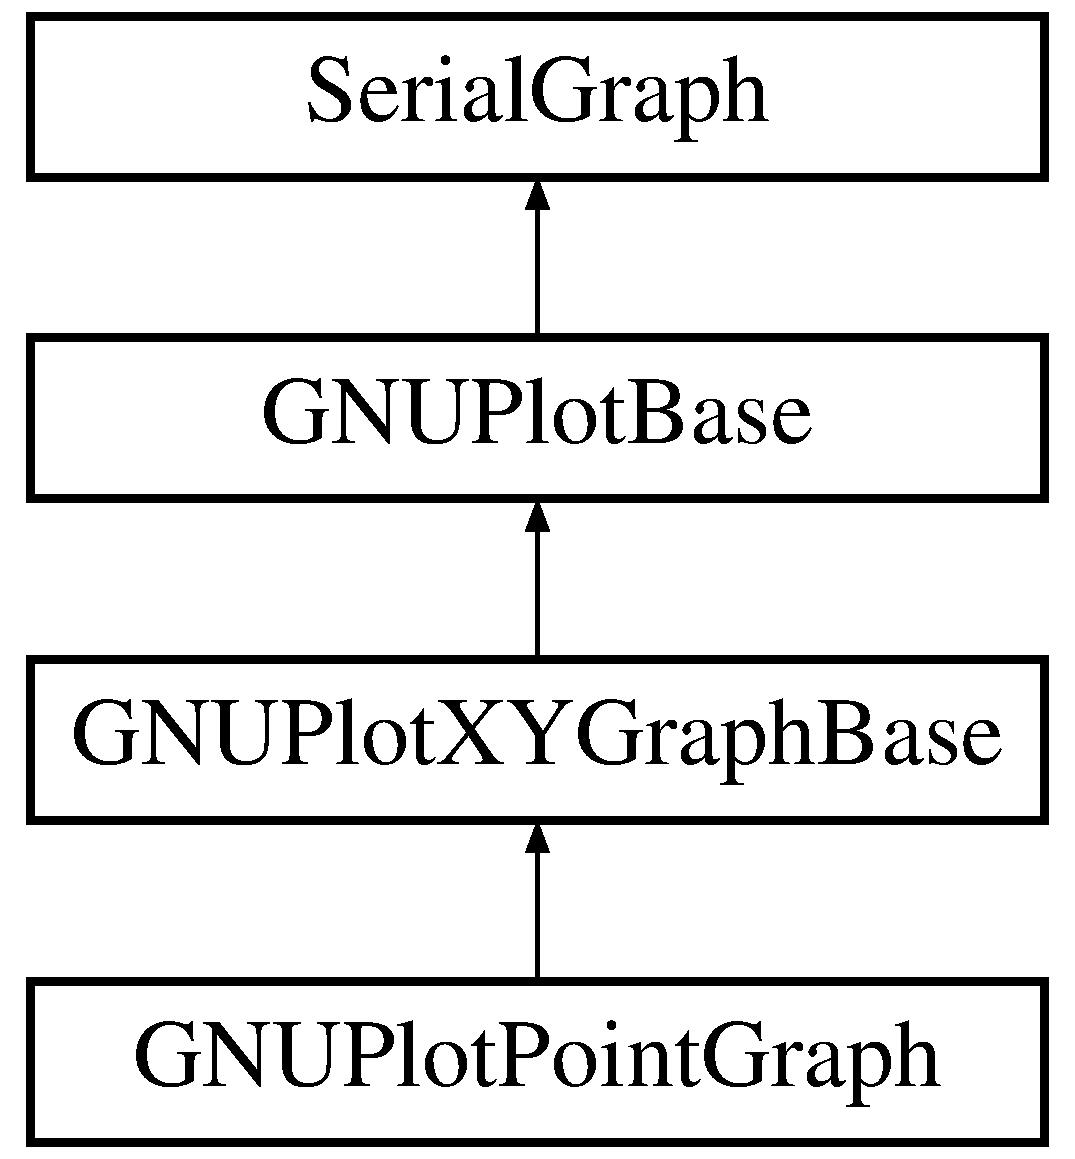
\includegraphics[height=4.000000cm]{class_g_n_u_plot_point_graph}
\end{center}
\end{figure}
\subsection*{Public Member Functions}
\begin{DoxyCompactItemize}
\item 
\hyperlink{class_g_n_u_plot_point_graph_a2b97fa221bf9012787cd20df14dc1c3c}{G\+N\+U\+Plot\+Point\+Graph} (Print $\ast$\+\_\+out\+Stream)
\item 
virtual \hyperlink{class_g_n_u_plot_point_graph_a41cd525a889e78bcfc3359f52a2afecb}{$\sim$\+G\+N\+U\+Plot\+Point\+Graph} ()
\item 
virtual \hyperlink{_serial_graph_8h_adc73bce6b7e6c4ecf37dde452d6a385e}{Graph\+Style} \hyperlink{class_g_n_u_plot_point_graph_aeeae395426112202d3617ff66d836c99}{get\+Graph\+Style} () const 
\item 
virtual void \hyperlink{class_g_n_u_plot_x_y_graph_base_a8389f830ff330dfb705e00d31053e130}{create\+Graph} ()
\item 
virtual void \hyperlink{class_g_n_u_plot_base_a4d4da234cfdeb99ec3228ef7b2df8a50}{new\+Graph} ()
\item 
virtual void \hyperlink{class_g_n_u_plot_base_aa4b0574c35fbee4dc5f25451eaf956dd}{finish\+Graph} ()
\item 
virtual void \hyperlink{class_g_n_u_plot_base_a219601bd41203477ae73a18d18dd7443}{print\+Comment\+Start} ()
\item 
virtual void \hyperlink{class_serial_graph_a28b020807c52c113685aa6a31f836c52}{enable\+Save\+Image\+File} (bool enabled)
\item 
virtual void \hyperlink{class_serial_graph_abf488e449d6d786bc01478793d0094ad}{set\+Show\+Grid} (bool enabled)
\item 
void \hyperlink{class_serial_graph_a4db09b008589914b71b2ee8b1873db7a}{set\+Title} (const \+\_\+\+\_\+\+Flash\+String\+Helper $\ast$title)
\item 
virtual void \hyperlink{class_serial_graph_ad726b2c84cec50c2d4bfe769e62a9bcd}{set\+Title} (const char $\ast$title)
\item 
void \hyperlink{class_serial_graph_afdb759a860c41de2fc4cfe78519b9fc0}{set\+X\+Axis\+Name} (const \+\_\+\+\_\+\+Flash\+String\+Helper $\ast$title)
\item 
virtual void \hyperlink{class_serial_graph_ac7f30036f5006091af51204a4d9efaf2}{set\+X\+Axis\+Name} (const char $\ast$name)
\item 
void \hyperlink{class_serial_graph_abfc46c15cf8e1b4362a7f51cb11c7bdb}{set\+Y\+Axis\+Name} (const \+\_\+\+\_\+\+Flash\+String\+Helper $\ast$title)
\item 
virtual void \hyperlink{class_serial_graph_ab0c675c8682959261f79dcf37b04148c}{set\+Y\+Axis\+Name} (const char $\ast$name)
\item 
virtual void \hyperlink{class_serial_graph_ae58de4fa4d391f1a2f411ce00dd74d93}{set\+X\+Axis\+Log} (byte scale)
\item 
virtual void \hyperlink{class_serial_graph_a444e38e8ef3784942ca6ee58940f7023}{set\+Y\+Axis\+Log} (byte scale)
\item 
void \hyperlink{class_serial_graph_a84d8e8ce9bff20e53ba738d1d34d3577}{set\+Series\+Name} (int \+\_\+n, const \+\_\+\+\_\+\+Flash\+String\+Helper $\ast$title)
\item 
virtual void \hyperlink{class_serial_graph_a9d67fbecbee6edb82646aa7ba5103046}{set\+Series\+Name} (int \+\_\+n, const char $\ast$name)
\item 
\hyperlink{struct_line_apperance}{Line\+Apperance} $\ast$ \hyperlink{class_serial_graph_a5a6008dc86a2101a58782929721a5b77}{get\+Line\+Apperance} (int \+\_\+n)
\item 
{\footnotesize template$<$typename Y\+T $>$ }\\void \hyperlink{class_serial_graph_afbcc26bd6bad7179d75379ac0f0d25f1}{plot\+Datum\+Y} (Y\+T y1)
\item 
{\footnotesize template$<$typename X\+T , typename Y\+T $>$ }\\void \hyperlink{class_serial_graph_a265b48fb0afe543e14cedb6619e3931e}{plot\+Datum\+X\+Y} (X\+T x, Y\+T y1)
\item 
{\footnotesize template$<$typename Y\+T $>$ }\\void \hyperlink{class_serial_graph_a56f584fa6316175bc9fbcb4f671f1c93}{plot\+Datum\+Yn} (Y\+T y1, Y\+T y2)
\item 
{\footnotesize template$<$typename Y\+T $>$ }\\void \hyperlink{class_serial_graph_ae755b026606e34c33c4aa8f10d8b5d9c}{plot\+Datum\+Yn} (Y\+T y1, Y\+T y2, Y\+T y3)
\item 
{\footnotesize template$<$typename Y\+T $>$ }\\void \hyperlink{class_serial_graph_a354feb95f91239699d3510c2ce5659b0}{plot\+Datum\+Yn} (Y\+T y1, Y\+T y2, Y\+T y3, Y\+T y4)
\item 
{\footnotesize template$<$typename Y\+T $>$ }\\void \hyperlink{class_serial_graph_ab0fff3fc1879e1cd6aadf24c913ff617}{plot\+Datum\+Yn} (Y\+T y1, Y\+T y2, Y\+T y3, Y\+T y4, Y\+T y5)
\item 
{\footnotesize template$<$typename X\+T , typename Y\+T $>$ }\\void \hyperlink{class_serial_graph_aa20b03efac52c18c50efc79c6459a9fc}{plot\+Datum\+Yn} (const Y\+T $\ast$y\+Vec, int \+\_\+n)
\item 
{\footnotesize template$<$typename X\+T , typename Y\+T $>$ }\\void \hyperlink{class_serial_graph_a79b721ca2be68969862869f96d6a6305}{plot\+Datum\+X\+Yn} (X\+T x, Y\+T y1, Y\+T y2)
\item 
{\footnotesize template$<$typename X\+T , typename Y\+T $>$ }\\void \hyperlink{class_serial_graph_a9fcea879f299a7d24be4ff9a38c53c26}{plot\+Datum\+X\+Yn} (X\+T x, Y\+T y1, Y\+T y2, Y\+T y3)
\item 
{\footnotesize template$<$typename X\+T , typename Y\+T $>$ }\\void \hyperlink{class_serial_graph_afd854b631604abe2014a1bb1beeeec52}{plot\+Datum\+X\+Yn} (X\+T x, Y\+T y1, Y\+T y2, Y\+T y3, Y\+T y4)
\item 
{\footnotesize template$<$typename X\+T , typename Y\+T $>$ }\\void \hyperlink{class_serial_graph_aa1bb6fa08a8bd06c074ac2a02b3f6fbc}{plot\+Datum\+X\+Yn} (X\+T x, Y\+T y1, Y\+T y2, Y\+T y3, Y\+T y4, Y\+T y5)
\item 
{\footnotesize template$<$typename X\+T , typename Y\+T $>$ }\\void \hyperlink{class_serial_graph_a3d7276c89235dc1aa176e2439ad9835b}{plot\+Datum\+X\+Yn} (X\+T x, const Y\+T $\ast$y\+Vec, int \+\_\+n)
\item 
{\footnotesize template$<$typename W\+T $>$ }\\void \hyperlink{class_serial_graph_aa72b48968e82a953dcdc6522bd04c7b4}{print} (const W\+T what)
\item 
{\footnotesize template$<$typename W\+T $>$ }\\void \hyperlink{class_serial_graph_a2005d103cb5a578053ef7838b3a8422d}{println} (const W\+T what)
\item 
{\footnotesize template$<$typename W\+T $>$ }\\void \hyperlink{class_serial_graph_a7237d928f67a14d5c9950d8c23c2a794}{print\+Comment} (const W\+T what)
\item 
{\footnotesize template$<$typename W\+T $>$ }\\void \hyperlink{class_serial_graph_a9b40aa22335fc26a6c29b16d278b26f8}{print\+Comment} (const W\+T $\ast$what)
\end{DoxyCompactItemize}
\subsection*{Public Attributes}
\begin{DoxyCompactItemize}
\item 
const byte \hyperlink{class_serial_graph_a1867ab3a93268646490fa7ba4f8b5680}{max\+String\+Size} = 128
\item 
const byte \hyperlink{class_serial_graph_a752a1429bd35687163fe11c5a2562bef}{max\+Series} = 8
\end{DoxyCompactItemize}
\subsection*{Protected Member Functions}
\begin{DoxyCompactItemize}
\item 
{\footnotesize template$<$typename T , typename U $>$ }\\void \hyperlink{class_g_n_u_plot_base_a03d371b0c6c7ef89064525438b22d52c}{set\+Variable} (T name, U value, bool quoted)
\item 
{\footnotesize template$<$typename T $>$ }\\void \hyperlink{class_g_n_u_plot_base_a3c8c8f68c13661d91bd844589e1a2a85}{set\+Variable} (T name)
\item 
{\footnotesize template$<$typename T $>$ }\\void \hyperlink{class_g_n_u_plot_base_af9b418bbcafb41d4d51b92018ca4f217}{unset\+Variable} (T name)
\item 
{\footnotesize template$<$typename T $>$ }\\void \hyperlink{class_g_n_u_plot_base_a68171bf36461e54e2b81384c112ad975}{set\+Varible\+By\+String\+\_\+null\+Safe} (T name, const char $\ast$text)
\item 
{\footnotesize template$<$typename T $>$ }\\void \hyperlink{class_g_n_u_plot_base_ae93c5de3241c2b6b6f703a202dc1d94b}{set\+Varible\+Flag\+By\+Boolean} (T name, bool value)
\item 
void \hyperlink{class_g_n_u_plot_base_ab5c851953dd140cc3ee936a5cd329200}{save\+Plot\+To\+Image\+File} (const char $\ast$title)
\item 
virtual void \hyperlink{class_g_n_u_plot_base_adaf91c191e4d889537d401faeb863485}{make\+Ready\+For\+Plot\+Data} ()
\item 
char $\ast$ \hyperlink{class_g_n_u_plot_base_a7f71f3c616b3a4a854f9118a04c40447}{malloc\+Basic\+File\+Name\+From\+Graph\+Title} ()
\item 
void \hyperlink{class_g_n_u_plot_base_a65ae2b3220034bce21c7feb39a632991}{print\+Title\+In\+Plot\+Command} (int series\+Num)
\item 
void \hyperlink{class_g_n_u_plot_base_ad057969aa7f8bdbe884d6a5d03a29722}{print\+Line\+Apperance} (\hyperlink{struct_line_apperance}{Line\+Apperance} apperance)
\item 
void \hyperlink{class_g_n_u_plot_base_ad7e8ef8d8e5eb80119fc0cce9be2d525}{print\+Log\+Axis\+Command} (const \+\_\+\+\_\+\+Flash\+String\+Helper $\ast$axis\+Name, byte log\+Scale)
\item 
virtual void \hyperlink{class_g_n_u_plot_base_ae204818b4e8dcd9d2f6b5426127ca2cf}{print\+Seperator} ()
\item 
virtual void \hyperlink{class_g_n_u_plot_base_ac2b48b822b6043392b514c9580b1661a}{print\+Start\+Datum} ()
\item 
virtual void \hyperlink{class_g_n_u_plot_base_aff02bc279e6c3cb83f2cdc7aa021268f}{print\+End\+Datum} ()
\item 
virtual void \hyperlink{class_g_n_u_plot_base_ad00a12fd681e4638fae005891fd72f38}{\+\_\+print\+Data\+Value} (const char $\ast$value)
\item 
virtual void \hyperlink{class_g_n_u_plot_base_aa6c6dfff0568dd99c0c28081c41b4433}{\+\_\+print\+Data\+Value} (char value)
\item 
virtual void \hyperlink{class_g_n_u_plot_base_a6f14fc040ff833c685ab09fc7917e059}{\+\_\+print\+Data\+Value} (bool value)
\item 
virtual void \hyperlink{class_serial_graph_a0c4d2c1239de3107d7332389183b05a1}{\+\_\+print\+Data\+Value} (const \+\_\+\+\_\+\+Flash\+String\+Helper $\ast$value)
\item 
virtual void \hyperlink{class_serial_graph_a58edf4683c600b6bfa1714b0f8dfc82c}{\+\_\+print\+Data\+Value} (int value)
\item 
virtual void \hyperlink{class_serial_graph_a9a4903d4fa26bb85ba5dd93c4365bcc2}{\+\_\+print\+Data\+Value} (long value)
\item 
virtual void \hyperlink{class_serial_graph_acada5333b96b65e31d8c76c3ab22905f}{\+\_\+print\+Data\+Value} (byte value)
\item 
virtual void \hyperlink{class_serial_graph_acd91cf0c3a0f49d4bdf18b447503da23}{\+\_\+print\+Data\+Value} (unsigned int value)
\item 
virtual void \hyperlink{class_serial_graph_a6dbfe61ee398e18c1b752a3748df9663}{\+\_\+print\+Data\+Value} (unsigned long value)
\item 
virtual void \hyperlink{class_serial_graph_a766d5838ede9c8fa998ce8664e5f92be}{\+\_\+print\+Data\+Value} (double value)
\item 
void \hyperlink{class_serial_graph_a760dd00474c9780c81ece7cdf621fc15}{init} ()
\item 
void \hyperlink{class_serial_graph_abd43150abedec26eef3994cd33035173}{ensure\+Ready\+To\+Recive\+Plot\+Data} ()
\item 
{\footnotesize template$<$typename T $>$ }\\void \hyperlink{class_serial_graph_a91e20c05c8cc612fd9ffd85880149264}{print\+Data\+Value} (T value)
\end{DoxyCompactItemize}
\subsection*{Protected Attributes}
\begin{DoxyCompactItemize}
\item 
bool \hyperlink{class_serial_graph_a24202e0a7a8bac5ec1cfd92bf796e078}{save\+File}
\item 
Print $\ast$ \hyperlink{class_serial_graph_aec32289a9393e98bf80d44406e5c207d}{out\+Stream}
\item 
bool \hyperlink{class_serial_graph_a4dbd9cf190c591fb4f2f46a50d937199}{x\+Axis\+Specified}
\item 
int \hyperlink{class_serial_graph_ab40c430e06102b9624736173d4a58596}{num\+Y\+Series}
\item 
bool \hyperlink{class_serial_graph_ad61d5ea29eacc1611c5addc94714f1e2}{show\+Grid}
\item 
char $\ast$ \hyperlink{class_serial_graph_a0b33d43c2bb54340ef1f90b5f76d7aea}{graph\+Title}
\item 
char $\ast$ \hyperlink{class_serial_graph_a5f5bf85ed361ff567d0888eaa73e269c}{x\+Axis\+Name}
\item 
char $\ast$ \hyperlink{class_serial_graph_a08452a56c74ec5f5473b64605d555339}{y\+Axis\+Name}
\item 
char $\ast$$\ast$ \hyperlink{class_serial_graph_a2307e40e27249f44bbe14776dc68c561}{series\+Names}
\item 
\hyperlink{struct_line_apperance}{Line\+Apperance} $\ast$ \hyperlink{class_serial_graph_a8d743f9eeeca69a988d2159a405e4253}{series\+Apperance}
\item 
byte \hyperlink{class_serial_graph_afc2ca72fdfe2bc5e3159c9e910a8f81e}{x\+Axis\+Log\+Scale}
\item 
byte \hyperlink{class_serial_graph_a1f0424857ec14c176747b3ddb0768eee}{y\+Axis\+Log\+Scale}
\end{DoxyCompactItemize}


\subsection{Detailed Description}
Specilisation of \hyperlink{class_g_n_u_plot_x_y_graph_base}{G\+N\+U\+Plot\+X\+Y\+Graph\+Base} to make a nice scatter plot. \hyperlink{class_g_n_u_plot_point_graph_aeeae395426112202d3617ff66d836c99}{G\+N\+U\+Plot\+Point\+Graph\+::get\+Graph\+Style()} alters the behaviour of \hyperlink{class_g_n_u_plot_x_y_graph_base_a8389f830ff330dfb705e00d31053e130}{G\+N\+U\+Plot\+X\+Y\+Graph\+Base\+::create\+Graph()} 

\subsection{Constructor \& Destructor Documentation}
\hypertarget{class_g_n_u_plot_point_graph_a2b97fa221bf9012787cd20df14dc1c3c}{}\index{G\+N\+U\+Plot\+Point\+Graph@{G\+N\+U\+Plot\+Point\+Graph}!G\+N\+U\+Plot\+Point\+Graph@{G\+N\+U\+Plot\+Point\+Graph}}
\index{G\+N\+U\+Plot\+Point\+Graph@{G\+N\+U\+Plot\+Point\+Graph}!G\+N\+U\+Plot\+Point\+Graph@{G\+N\+U\+Plot\+Point\+Graph}}
\subsubsection[{G\+N\+U\+Plot\+Point\+Graph(\+Print $\ast$\+\_\+out\+Stream)}]{\setlength{\rightskip}{0pt plus 5cm}G\+N\+U\+Plot\+Point\+Graph\+::\+G\+N\+U\+Plot\+Point\+Graph (
\begin{DoxyParamCaption}
\item[{Print $\ast$}]{\+\_\+out\+Stream}
\end{DoxyParamCaption}
)\hspace{0.3cm}{\ttfamily [inline]}}\label{class_g_n_u_plot_point_graph_a2b97fa221bf9012787cd20df14dc1c3c}
\hypertarget{class_g_n_u_plot_point_graph_a41cd525a889e78bcfc3359f52a2afecb}{}\index{G\+N\+U\+Plot\+Point\+Graph@{G\+N\+U\+Plot\+Point\+Graph}!````~G\+N\+U\+Plot\+Point\+Graph@{$\sim$\+G\+N\+U\+Plot\+Point\+Graph}}
\index{````~G\+N\+U\+Plot\+Point\+Graph@{$\sim$\+G\+N\+U\+Plot\+Point\+Graph}!G\+N\+U\+Plot\+Point\+Graph@{G\+N\+U\+Plot\+Point\+Graph}}
\subsubsection[{$\sim$\+G\+N\+U\+Plot\+Point\+Graph()}]{\setlength{\rightskip}{0pt plus 5cm}virtual G\+N\+U\+Plot\+Point\+Graph\+::$\sim$\+G\+N\+U\+Plot\+Point\+Graph (
\begin{DoxyParamCaption}
{}
\end{DoxyParamCaption}
)\hspace{0.3cm}{\ttfamily [inline]}, {\ttfamily [virtual]}}\label{class_g_n_u_plot_point_graph_a41cd525a889e78bcfc3359f52a2afecb}


\subsection{Member Function Documentation}
\hypertarget{class_g_n_u_plot_base_ad00a12fd681e4638fae005891fd72f38}{}\index{G\+N\+U\+Plot\+Point\+Graph@{G\+N\+U\+Plot\+Point\+Graph}!\+\_\+print\+Data\+Value@{\+\_\+print\+Data\+Value}}
\index{\+\_\+print\+Data\+Value@{\+\_\+print\+Data\+Value}!G\+N\+U\+Plot\+Point\+Graph@{G\+N\+U\+Plot\+Point\+Graph}}
\subsubsection[{\+\_\+print\+Data\+Value(const char $\ast$value)}]{\setlength{\rightskip}{0pt plus 5cm}void G\+N\+U\+Plot\+Base\+::\+\_\+print\+Data\+Value (
\begin{DoxyParamCaption}
\item[{const char $\ast$}]{value}
\end{DoxyParamCaption}
)\hspace{0.3cm}{\ttfamily [protected]}, {\ttfamily [virtual]}, {\ttfamily [inherited]}}\label{class_g_n_u_plot_base_ad00a12fd681e4638fae005891fd72f38}
Override a put appropriate quotes around strings etc. 
\begin{DoxyParams}{Parameters}
{\em value} & What to print. \\
\hline
\end{DoxyParams}


Reimplemented from \hyperlink{class_serial_graph_a8252997dd4bad0251d437d6dd097bffb}{Serial\+Graph}.

\hypertarget{class_g_n_u_plot_base_aa6c6dfff0568dd99c0c28081c41b4433}{}\index{G\+N\+U\+Plot\+Point\+Graph@{G\+N\+U\+Plot\+Point\+Graph}!\+\_\+print\+Data\+Value@{\+\_\+print\+Data\+Value}}
\index{\+\_\+print\+Data\+Value@{\+\_\+print\+Data\+Value}!G\+N\+U\+Plot\+Point\+Graph@{G\+N\+U\+Plot\+Point\+Graph}}
\subsubsection[{\+\_\+print\+Data\+Value(char value)}]{\setlength{\rightskip}{0pt plus 5cm}virtual void G\+N\+U\+Plot\+Base\+::\+\_\+print\+Data\+Value (
\begin{DoxyParamCaption}
\item[{char}]{value}
\end{DoxyParamCaption}
)\hspace{0.3cm}{\ttfamily [inline]}, {\ttfamily [protected]}, {\ttfamily [virtual]}, {\ttfamily [inherited]}}\label{class_g_n_u_plot_base_aa6c6dfff0568dd99c0c28081c41b4433}
Override for customised value output. 
\begin{DoxyParams}{Parameters}
{\em value} & What to print. \\
\hline
\end{DoxyParams}


Reimplemented from \hyperlink{class_serial_graph_af3fbf7a9201f71cd6bad7e4337092fb6}{Serial\+Graph}.

\hypertarget{class_g_n_u_plot_base_a6f14fc040ff833c685ab09fc7917e059}{}\index{G\+N\+U\+Plot\+Point\+Graph@{G\+N\+U\+Plot\+Point\+Graph}!\+\_\+print\+Data\+Value@{\+\_\+print\+Data\+Value}}
\index{\+\_\+print\+Data\+Value@{\+\_\+print\+Data\+Value}!G\+N\+U\+Plot\+Point\+Graph@{G\+N\+U\+Plot\+Point\+Graph}}
\subsubsection[{\+\_\+print\+Data\+Value(bool value)}]{\setlength{\rightskip}{0pt plus 5cm}virtual void G\+N\+U\+Plot\+Base\+::\+\_\+print\+Data\+Value (
\begin{DoxyParamCaption}
\item[{bool}]{value}
\end{DoxyParamCaption}
)\hspace{0.3cm}{\ttfamily [inline]}, {\ttfamily [protected]}, {\ttfamily [virtual]}, {\ttfamily [inherited]}}\label{class_g_n_u_plot_base_a6f14fc040ff833c685ab09fc7917e059}
Override for customised value output. 
\begin{DoxyParams}{Parameters}
{\em value} & What to print. \\
\hline
\end{DoxyParams}


Reimplemented from \hyperlink{class_serial_graph_aed9ff95634ace3d190863ea9d15c10da}{Serial\+Graph}.

\hypertarget{class_serial_graph_a0c4d2c1239de3107d7332389183b05a1}{}\index{G\+N\+U\+Plot\+Point\+Graph@{G\+N\+U\+Plot\+Point\+Graph}!\+\_\+print\+Data\+Value@{\+\_\+print\+Data\+Value}}
\index{\+\_\+print\+Data\+Value@{\+\_\+print\+Data\+Value}!G\+N\+U\+Plot\+Point\+Graph@{G\+N\+U\+Plot\+Point\+Graph}}
\subsubsection[{\+\_\+print\+Data\+Value(const \+\_\+\+\_\+\+Flash\+String\+Helper $\ast$value)}]{\setlength{\rightskip}{0pt plus 5cm}virtual void Serial\+Graph\+::\+\_\+print\+Data\+Value (
\begin{DoxyParamCaption}
\item[{const \+\_\+\+\_\+\+Flash\+String\+Helper $\ast$}]{value}
\end{DoxyParamCaption}
)\hspace{0.3cm}{\ttfamily [inline]}, {\ttfamily [protected]}, {\ttfamily [virtual]}, {\ttfamily [inherited]}}\label{class_serial_graph_a0c4d2c1239de3107d7332389183b05a1}
This just calls \hyperlink{class_serial_graph_a8252997dd4bad0251d437d6dd097bffb}{\+\_\+print\+Data\+Value(const char $\ast$value)} so probably alter that instead. 
\begin{DoxyParams}{Parameters}
{\em value} & What to print. \\
\hline
\end{DoxyParams}
\hypertarget{class_serial_graph_a58edf4683c600b6bfa1714b0f8dfc82c}{}\index{G\+N\+U\+Plot\+Point\+Graph@{G\+N\+U\+Plot\+Point\+Graph}!\+\_\+print\+Data\+Value@{\+\_\+print\+Data\+Value}}
\index{\+\_\+print\+Data\+Value@{\+\_\+print\+Data\+Value}!G\+N\+U\+Plot\+Point\+Graph@{G\+N\+U\+Plot\+Point\+Graph}}
\subsubsection[{\+\_\+print\+Data\+Value(int value)}]{\setlength{\rightskip}{0pt plus 5cm}virtual void Serial\+Graph\+::\+\_\+print\+Data\+Value (
\begin{DoxyParamCaption}
\item[{int}]{value}
\end{DoxyParamCaption}
)\hspace{0.3cm}{\ttfamily [inline]}, {\ttfamily [protected]}, {\ttfamily [virtual]}, {\ttfamily [inherited]}}\label{class_serial_graph_a58edf4683c600b6bfa1714b0f8dfc82c}
Override for customised value output. 
\begin{DoxyParams}{Parameters}
{\em value} & What to print. \\
\hline
\end{DoxyParams}
\hypertarget{class_serial_graph_a9a4903d4fa26bb85ba5dd93c4365bcc2}{}\index{G\+N\+U\+Plot\+Point\+Graph@{G\+N\+U\+Plot\+Point\+Graph}!\+\_\+print\+Data\+Value@{\+\_\+print\+Data\+Value}}
\index{\+\_\+print\+Data\+Value@{\+\_\+print\+Data\+Value}!G\+N\+U\+Plot\+Point\+Graph@{G\+N\+U\+Plot\+Point\+Graph}}
\subsubsection[{\+\_\+print\+Data\+Value(long value)}]{\setlength{\rightskip}{0pt plus 5cm}virtual void Serial\+Graph\+::\+\_\+print\+Data\+Value (
\begin{DoxyParamCaption}
\item[{long}]{value}
\end{DoxyParamCaption}
)\hspace{0.3cm}{\ttfamily [inline]}, {\ttfamily [protected]}, {\ttfamily [virtual]}, {\ttfamily [inherited]}}\label{class_serial_graph_a9a4903d4fa26bb85ba5dd93c4365bcc2}
Override for customised value output. 
\begin{DoxyParams}{Parameters}
{\em value} & What to print. \\
\hline
\end{DoxyParams}
\hypertarget{class_serial_graph_acada5333b96b65e31d8c76c3ab22905f}{}\index{G\+N\+U\+Plot\+Point\+Graph@{G\+N\+U\+Plot\+Point\+Graph}!\+\_\+print\+Data\+Value@{\+\_\+print\+Data\+Value}}
\index{\+\_\+print\+Data\+Value@{\+\_\+print\+Data\+Value}!G\+N\+U\+Plot\+Point\+Graph@{G\+N\+U\+Plot\+Point\+Graph}}
\subsubsection[{\+\_\+print\+Data\+Value(byte value)}]{\setlength{\rightskip}{0pt plus 5cm}virtual void Serial\+Graph\+::\+\_\+print\+Data\+Value (
\begin{DoxyParamCaption}
\item[{byte}]{value}
\end{DoxyParamCaption}
)\hspace{0.3cm}{\ttfamily [inline]}, {\ttfamily [protected]}, {\ttfamily [virtual]}, {\ttfamily [inherited]}}\label{class_serial_graph_acada5333b96b65e31d8c76c3ab22905f}
Override for customised value output. 
\begin{DoxyParams}{Parameters}
{\em value} & What to print. \\
\hline
\end{DoxyParams}
\hypertarget{class_serial_graph_acd91cf0c3a0f49d4bdf18b447503da23}{}\index{G\+N\+U\+Plot\+Point\+Graph@{G\+N\+U\+Plot\+Point\+Graph}!\+\_\+print\+Data\+Value@{\+\_\+print\+Data\+Value}}
\index{\+\_\+print\+Data\+Value@{\+\_\+print\+Data\+Value}!G\+N\+U\+Plot\+Point\+Graph@{G\+N\+U\+Plot\+Point\+Graph}}
\subsubsection[{\+\_\+print\+Data\+Value(unsigned int value)}]{\setlength{\rightskip}{0pt plus 5cm}virtual void Serial\+Graph\+::\+\_\+print\+Data\+Value (
\begin{DoxyParamCaption}
\item[{unsigned int}]{value}
\end{DoxyParamCaption}
)\hspace{0.3cm}{\ttfamily [inline]}, {\ttfamily [protected]}, {\ttfamily [virtual]}, {\ttfamily [inherited]}}\label{class_serial_graph_acd91cf0c3a0f49d4bdf18b447503da23}
Override for customised value output. 
\begin{DoxyParams}{Parameters}
{\em value} & What to print. \\
\hline
\end{DoxyParams}
\hypertarget{class_serial_graph_a6dbfe61ee398e18c1b752a3748df9663}{}\index{G\+N\+U\+Plot\+Point\+Graph@{G\+N\+U\+Plot\+Point\+Graph}!\+\_\+print\+Data\+Value@{\+\_\+print\+Data\+Value}}
\index{\+\_\+print\+Data\+Value@{\+\_\+print\+Data\+Value}!G\+N\+U\+Plot\+Point\+Graph@{G\+N\+U\+Plot\+Point\+Graph}}
\subsubsection[{\+\_\+print\+Data\+Value(unsigned long value)}]{\setlength{\rightskip}{0pt plus 5cm}virtual void Serial\+Graph\+::\+\_\+print\+Data\+Value (
\begin{DoxyParamCaption}
\item[{unsigned long}]{value}
\end{DoxyParamCaption}
)\hspace{0.3cm}{\ttfamily [inline]}, {\ttfamily [protected]}, {\ttfamily [virtual]}, {\ttfamily [inherited]}}\label{class_serial_graph_a6dbfe61ee398e18c1b752a3748df9663}
Override for customised value output. 
\begin{DoxyParams}{Parameters}
{\em value} & What to print. \\
\hline
\end{DoxyParams}
\hypertarget{class_serial_graph_a766d5838ede9c8fa998ce8664e5f92be}{}\index{G\+N\+U\+Plot\+Point\+Graph@{G\+N\+U\+Plot\+Point\+Graph}!\+\_\+print\+Data\+Value@{\+\_\+print\+Data\+Value}}
\index{\+\_\+print\+Data\+Value@{\+\_\+print\+Data\+Value}!G\+N\+U\+Plot\+Point\+Graph@{G\+N\+U\+Plot\+Point\+Graph}}
\subsubsection[{\+\_\+print\+Data\+Value(double value)}]{\setlength{\rightskip}{0pt plus 5cm}virtual void Serial\+Graph\+::\+\_\+print\+Data\+Value (
\begin{DoxyParamCaption}
\item[{double}]{value}
\end{DoxyParamCaption}
)\hspace{0.3cm}{\ttfamily [inline]}, {\ttfamily [protected]}, {\ttfamily [virtual]}, {\ttfamily [inherited]}}\label{class_serial_graph_a766d5838ede9c8fa998ce8664e5f92be}
Override for customised value output. 
\begin{DoxyParams}{Parameters}
{\em value} & What to print. \\
\hline
\end{DoxyParams}
\hypertarget{class_g_n_u_plot_x_y_graph_base_a8389f830ff330dfb705e00d31053e130}{}\index{G\+N\+U\+Plot\+Point\+Graph@{G\+N\+U\+Plot\+Point\+Graph}!create\+Graph@{create\+Graph}}
\index{create\+Graph@{create\+Graph}!G\+N\+U\+Plot\+Point\+Graph@{G\+N\+U\+Plot\+Point\+Graph}}
\subsubsection[{create\+Graph()}]{\setlength{\rightskip}{0pt plus 5cm}void G\+N\+U\+Plot\+X\+Y\+Graph\+Base\+::create\+Graph (
\begin{DoxyParamCaption}
{}
\end{DoxyParamCaption}
)\hspace{0.3cm}{\ttfamily [virtual]}, {\ttfamily [inherited]}}\label{class_g_n_u_plot_x_y_graph_base_a8389f830ff330dfb705e00d31053e130}


Implements \hyperlink{class_g_n_u_plot_base_ad877f207d43e6f9cd0aa0ef241e31c24}{G\+N\+U\+Plot\+Base}.

\hypertarget{class_serial_graph_a28b020807c52c113685aa6a31f836c52}{}\index{G\+N\+U\+Plot\+Point\+Graph@{G\+N\+U\+Plot\+Point\+Graph}!enable\+Save\+Image\+File@{enable\+Save\+Image\+File}}
\index{enable\+Save\+Image\+File@{enable\+Save\+Image\+File}!G\+N\+U\+Plot\+Point\+Graph@{G\+N\+U\+Plot\+Point\+Graph}}
\subsubsection[{enable\+Save\+Image\+File(bool enabled)}]{\setlength{\rightskip}{0pt plus 5cm}virtual void Serial\+Graph\+::enable\+Save\+Image\+File (
\begin{DoxyParamCaption}
\item[{bool}]{enabled}
\end{DoxyParamCaption}
)\hspace{0.3cm}{\ttfamily [inline]}, {\ttfamily [virtual]}, {\ttfamily [inherited]}}\label{class_serial_graph_a28b020807c52c113685aa6a31f836c52}
Set to true if an image file should be saved. \begin{DoxyNote}{Note}
Filename will be based on graph title. This is done to save memory. Final filename has some extra validation performed to conform with filename rules aplicable to modern operating systems (excluding 8 char limit). 
\end{DoxyNote}
\hypertarget{class_serial_graph_abd43150abedec26eef3994cd33035173}{}\index{G\+N\+U\+Plot\+Point\+Graph@{G\+N\+U\+Plot\+Point\+Graph}!ensure\+Ready\+To\+Recive\+Plot\+Data@{ensure\+Ready\+To\+Recive\+Plot\+Data}}
\index{ensure\+Ready\+To\+Recive\+Plot\+Data@{ensure\+Ready\+To\+Recive\+Plot\+Data}!G\+N\+U\+Plot\+Point\+Graph@{G\+N\+U\+Plot\+Point\+Graph}}
\subsubsection[{ensure\+Ready\+To\+Recive\+Plot\+Data()}]{\setlength{\rightskip}{0pt plus 5cm}void Serial\+Graph\+::ensure\+Ready\+To\+Recive\+Plot\+Data (
\begin{DoxyParamCaption}
{}
\end{DoxyParamCaption}
)\hspace{0.3cm}{\ttfamily [protected]}, {\ttfamily [inherited]}}\label{class_serial_graph_abd43150abedec26eef3994cd33035173}
Called by every plot command prior to sending data. it\textquotesingle{}s function is to call \hyperlink{class_serial_graph_a898cf274c886e0ff45e90d3f21f0a6cc}{make\+Ready\+For\+Plot\+Data()} the first time it is called. 
\begin{DoxyParams}{Parameters}
{\em value} & What to print. \\
\hline
\end{DoxyParams}
\hypertarget{class_g_n_u_plot_base_aa4b0574c35fbee4dc5f25451eaf956dd}{}\index{G\+N\+U\+Plot\+Point\+Graph@{G\+N\+U\+Plot\+Point\+Graph}!finish\+Graph@{finish\+Graph}}
\index{finish\+Graph@{finish\+Graph}!G\+N\+U\+Plot\+Point\+Graph@{G\+N\+U\+Plot\+Point\+Graph}}
\subsubsection[{finish\+Graph()}]{\setlength{\rightskip}{0pt plus 5cm}void G\+N\+U\+Plot\+Base\+::finish\+Graph (
\begin{DoxyParamCaption}
{}
\end{DoxyParamCaption}
)\hspace{0.3cm}{\ttfamily [virtual]}, {\ttfamily [inherited]}}\label{class_g_n_u_plot_base_aa4b0574c35fbee4dc5f25451eaf956dd}
Serial output that finishes the plot, saves file, updates display etc. 

Implements \hyperlink{class_serial_graph_a8054ce989a1788bd35d2fde56081c88c}{Serial\+Graph}.

\hypertarget{class_g_n_u_plot_point_graph_aeeae395426112202d3617ff66d836c99}{}\index{G\+N\+U\+Plot\+Point\+Graph@{G\+N\+U\+Plot\+Point\+Graph}!get\+Graph\+Style@{get\+Graph\+Style}}
\index{get\+Graph\+Style@{get\+Graph\+Style}!G\+N\+U\+Plot\+Point\+Graph@{G\+N\+U\+Plot\+Point\+Graph}}
\subsubsection[{get\+Graph\+Style() const }]{\setlength{\rightskip}{0pt plus 5cm}virtual {\bf Graph\+Style} G\+N\+U\+Plot\+Point\+Graph\+::get\+Graph\+Style (
\begin{DoxyParamCaption}
{}
\end{DoxyParamCaption}
) const\hspace{0.3cm}{\ttfamily [inline]}, {\ttfamily [virtual]}}\label{class_g_n_u_plot_point_graph_aeeae395426112202d3617ff66d836c99}
Returns the Graph\+Style of the current object. 

Implements \hyperlink{class_serial_graph_a2ab97096fffdf429bfa271b9fd4c642a}{Serial\+Graph}.

\hypertarget{class_serial_graph_a5a6008dc86a2101a58782929721a5b77}{}\index{G\+N\+U\+Plot\+Point\+Graph@{G\+N\+U\+Plot\+Point\+Graph}!get\+Line\+Apperance@{get\+Line\+Apperance}}
\index{get\+Line\+Apperance@{get\+Line\+Apperance}!G\+N\+U\+Plot\+Point\+Graph@{G\+N\+U\+Plot\+Point\+Graph}}
\subsubsection[{get\+Line\+Apperance(int \+\_\+n)}]{\setlength{\rightskip}{0pt plus 5cm}{\bf Line\+Apperance}$\ast$ Serial\+Graph\+::get\+Line\+Apperance (
\begin{DoxyParamCaption}
\item[{int}]{\+\_\+n}
\end{DoxyParamCaption}
)\hspace{0.3cm}{\ttfamily [inline]}, {\ttfamily [inherited]}}\label{class_serial_graph_a5a6008dc86a2101a58782929721a5b77}
Gets a structure that controls apperance of a series (called a \hyperlink{struct_line_apperance}{Line\+Apperance}). It is intended that you directly modify the structure returned, there is no set\+Line\+Apperance. See the struct \hyperlink{struct_line_apperance}{Line\+Apperance} for more.


\begin{DoxyParams}{Parameters}
{\em \+\_\+n} & Series number to alter.\\
\hline
\end{DoxyParams}
\begin{DoxyNote}{Note}
Behaviour on \+\_\+n $>$ max\+Series, is to just override the last possible series entry. 
\end{DoxyNote}
\hypertarget{class_serial_graph_a760dd00474c9780c81ece7cdf621fc15}{}\index{G\+N\+U\+Plot\+Point\+Graph@{G\+N\+U\+Plot\+Point\+Graph}!init@{init}}
\index{init@{init}!G\+N\+U\+Plot\+Point\+Graph@{G\+N\+U\+Plot\+Point\+Graph}}
\subsubsection[{init()}]{\setlength{\rightskip}{0pt plus 5cm}void Serial\+Graph\+::init (
\begin{DoxyParamCaption}
{}
\end{DoxyParamCaption}
)\hspace{0.3cm}{\ttfamily [protected]}, {\ttfamily [inherited]}}\label{class_serial_graph_a760dd00474c9780c81ece7cdf621fc15}
Brings the class to its default state. Called by the constructor and \hyperlink{class_serial_graph_a44d34593c56aa67142ccd9fcc0a1da86}{new\+Graph()}. \hypertarget{class_g_n_u_plot_base_adaf91c191e4d889537d401faeb863485}{}\index{G\+N\+U\+Plot\+Point\+Graph@{G\+N\+U\+Plot\+Point\+Graph}!make\+Ready\+For\+Plot\+Data@{make\+Ready\+For\+Plot\+Data}}
\index{make\+Ready\+For\+Plot\+Data@{make\+Ready\+For\+Plot\+Data}!G\+N\+U\+Plot\+Point\+Graph@{G\+N\+U\+Plot\+Point\+Graph}}
\subsubsection[{make\+Ready\+For\+Plot\+Data()}]{\setlength{\rightskip}{0pt plus 5cm}void G\+N\+U\+Plot\+Base\+::make\+Ready\+For\+Plot\+Data (
\begin{DoxyParamCaption}
{}
\end{DoxyParamCaption}
)\hspace{0.3cm}{\ttfamily [protected]}, {\ttfamily [virtual]}, {\ttfamily [inherited]}}\label{class_g_n_u_plot_base_adaf91c191e4d889537d401faeb863485}
Called by ensure\+Ready\+To\+Recive\+Plot\+Data, if the first plot command is encountered. \begin{DoxyNote}{Note}
A concrete class should override this. 
\end{DoxyNote}


Reimplemented from \hyperlink{class_serial_graph_a898cf274c886e0ff45e90d3f21f0a6cc}{Serial\+Graph}.

\hypertarget{class_g_n_u_plot_base_a7f71f3c616b3a4a854f9118a04c40447}{}\index{G\+N\+U\+Plot\+Point\+Graph@{G\+N\+U\+Plot\+Point\+Graph}!malloc\+Basic\+File\+Name\+From\+Graph\+Title@{malloc\+Basic\+File\+Name\+From\+Graph\+Title}}
\index{malloc\+Basic\+File\+Name\+From\+Graph\+Title@{malloc\+Basic\+File\+Name\+From\+Graph\+Title}!G\+N\+U\+Plot\+Point\+Graph@{G\+N\+U\+Plot\+Point\+Graph}}
\subsubsection[{malloc\+Basic\+File\+Name\+From\+Graph\+Title()}]{\setlength{\rightskip}{0pt plus 5cm}char $\ast$ G\+N\+U\+Plot\+Base\+::malloc\+Basic\+File\+Name\+From\+Graph\+Title (
\begin{DoxyParamCaption}
{}
\end{DoxyParamCaption}
)\hspace{0.3cm}{\ttfamily [protected]}, {\ttfamily [inherited]}}\label{class_g_n_u_plot_base_a7f71f3c616b3a4a854f9118a04c40447}
\hypertarget{class_g_n_u_plot_base_a4d4da234cfdeb99ec3228ef7b2df8a50}{}\index{G\+N\+U\+Plot\+Point\+Graph@{G\+N\+U\+Plot\+Point\+Graph}!new\+Graph@{new\+Graph}}
\index{new\+Graph@{new\+Graph}!G\+N\+U\+Plot\+Point\+Graph@{G\+N\+U\+Plot\+Point\+Graph}}
\subsubsection[{new\+Graph()}]{\setlength{\rightskip}{0pt plus 5cm}void G\+N\+U\+Plot\+Base\+::new\+Graph (
\begin{DoxyParamCaption}
{}
\end{DoxyParamCaption}
)\hspace{0.3cm}{\ttfamily [virtual]}, {\ttfamily [inherited]}}\label{class_g_n_u_plot_base_a4d4da234cfdeb99ec3228ef7b2df8a50}
Serial output that establishes a new graph. This should also call \hyperlink{class_serial_graph_a760dd00474c9780c81ece7cdf621fc15}{init()}, to reset the class. \begin{DoxyNote}{Note}
\+: If you wan\textquotesingle{}t a \char`\"{}memory breather\char`\"{} between plots, calling this method frees all series names, titles etc. 
\end{DoxyNote}


Implements \hyperlink{class_serial_graph_a44d34593c56aa67142ccd9fcc0a1da86}{Serial\+Graph}.

\hypertarget{class_serial_graph_a265b48fb0afe543e14cedb6619e3931e}{}\index{G\+N\+U\+Plot\+Point\+Graph@{G\+N\+U\+Plot\+Point\+Graph}!plot\+Datum\+X\+Y@{plot\+Datum\+X\+Y}}
\index{plot\+Datum\+X\+Y@{plot\+Datum\+X\+Y}!G\+N\+U\+Plot\+Point\+Graph@{G\+N\+U\+Plot\+Point\+Graph}}
\subsubsection[{plot\+Datum\+X\+Y(\+X\+T x, Y\+T y1)}]{\setlength{\rightskip}{0pt plus 5cm}template$<$typename X\+T , typename Y\+T $>$ void Serial\+Graph\+::plot\+Datum\+X\+Y (
\begin{DoxyParamCaption}
\item[{X\+T}]{x, }
\item[{Y\+T}]{y1}
\end{DoxyParamCaption}
)\hspace{0.3cm}{\ttfamily [inline]}, {\ttfamily [inherited]}}\label{class_serial_graph_a265b48fb0afe543e14cedb6619e3931e}
Outputs a point to be plotted. All Y values must be of the same type.

\begin{DoxyNote}{Note}
The first time this is called after \hyperlink{class_serial_graph_a44d34593c56aa67142ccd9fcc0a1da86}{new\+Graph()}, \hyperlink{class_serial_graph_a898cf274c886e0ff45e90d3f21f0a6cc}{make\+Ready\+For\+Plot\+Data()} will be called. 

The following feilds automatically set\+: x\+Axis\+Specified; num\+Y\+Series; 
\end{DoxyNote}
\hypertarget{class_serial_graph_a79b721ca2be68969862869f96d6a6305}{}\index{G\+N\+U\+Plot\+Point\+Graph@{G\+N\+U\+Plot\+Point\+Graph}!plot\+Datum\+X\+Yn@{plot\+Datum\+X\+Yn}}
\index{plot\+Datum\+X\+Yn@{plot\+Datum\+X\+Yn}!G\+N\+U\+Plot\+Point\+Graph@{G\+N\+U\+Plot\+Point\+Graph}}
\subsubsection[{plot\+Datum\+X\+Yn(\+X\+T x, Y\+T y1, Y\+T y2)}]{\setlength{\rightskip}{0pt plus 5cm}template$<$typename X\+T , typename Y\+T $>$ void Serial\+Graph\+::plot\+Datum\+X\+Yn (
\begin{DoxyParamCaption}
\item[{X\+T}]{x, }
\item[{Y\+T}]{y1, }
\item[{Y\+T}]{y2}
\end{DoxyParamCaption}
)\hspace{0.3cm}{\ttfamily [inline]}, {\ttfamily [inherited]}}\label{class_serial_graph_a79b721ca2be68969862869f96d6a6305}
Outputs a point to be plotted. All Y values must be of the same type.

\begin{DoxyNote}{Note}
The first time this is called after \hyperlink{class_serial_graph_a44d34593c56aa67142ccd9fcc0a1da86}{new\+Graph()}, \hyperlink{class_serial_graph_a898cf274c886e0ff45e90d3f21f0a6cc}{make\+Ready\+For\+Plot\+Data()} will be called. 

The following feilds automatically set\+: x\+Axis\+Specified; num\+Y\+Series; 
\end{DoxyNote}
\hypertarget{class_serial_graph_a9fcea879f299a7d24be4ff9a38c53c26}{}\index{G\+N\+U\+Plot\+Point\+Graph@{G\+N\+U\+Plot\+Point\+Graph}!plot\+Datum\+X\+Yn@{plot\+Datum\+X\+Yn}}
\index{plot\+Datum\+X\+Yn@{plot\+Datum\+X\+Yn}!G\+N\+U\+Plot\+Point\+Graph@{G\+N\+U\+Plot\+Point\+Graph}}
\subsubsection[{plot\+Datum\+X\+Yn(\+X\+T x, Y\+T y1, Y\+T y2, Y\+T y3)}]{\setlength{\rightskip}{0pt plus 5cm}template$<$typename X\+T , typename Y\+T $>$ void Serial\+Graph\+::plot\+Datum\+X\+Yn (
\begin{DoxyParamCaption}
\item[{X\+T}]{x, }
\item[{Y\+T}]{y1, }
\item[{Y\+T}]{y2, }
\item[{Y\+T}]{y3}
\end{DoxyParamCaption}
)\hspace{0.3cm}{\ttfamily [inline]}, {\ttfamily [inherited]}}\label{class_serial_graph_a9fcea879f299a7d24be4ff9a38c53c26}
Outputs a point to be plotted. All Y values must be of the same type.

\begin{DoxyNote}{Note}
The first time this is called after \hyperlink{class_serial_graph_a44d34593c56aa67142ccd9fcc0a1da86}{new\+Graph()}, \hyperlink{class_serial_graph_a898cf274c886e0ff45e90d3f21f0a6cc}{make\+Ready\+For\+Plot\+Data()} will be called. 

The following feilds automatically set\+: x\+Axis\+Specified; num\+Y\+Series; 
\end{DoxyNote}
\hypertarget{class_serial_graph_afd854b631604abe2014a1bb1beeeec52}{}\index{G\+N\+U\+Plot\+Point\+Graph@{G\+N\+U\+Plot\+Point\+Graph}!plot\+Datum\+X\+Yn@{plot\+Datum\+X\+Yn}}
\index{plot\+Datum\+X\+Yn@{plot\+Datum\+X\+Yn}!G\+N\+U\+Plot\+Point\+Graph@{G\+N\+U\+Plot\+Point\+Graph}}
\subsubsection[{plot\+Datum\+X\+Yn(\+X\+T x, Y\+T y1, Y\+T y2, Y\+T y3, Y\+T y4)}]{\setlength{\rightskip}{0pt plus 5cm}template$<$typename X\+T , typename Y\+T $>$ void Serial\+Graph\+::plot\+Datum\+X\+Yn (
\begin{DoxyParamCaption}
\item[{X\+T}]{x, }
\item[{Y\+T}]{y1, }
\item[{Y\+T}]{y2, }
\item[{Y\+T}]{y3, }
\item[{Y\+T}]{y4}
\end{DoxyParamCaption}
)\hspace{0.3cm}{\ttfamily [inline]}, {\ttfamily [inherited]}}\label{class_serial_graph_afd854b631604abe2014a1bb1beeeec52}
Outputs a point to be plotted. All Y values must be of the same type.

\begin{DoxyNote}{Note}
The first time this is called after \hyperlink{class_serial_graph_a44d34593c56aa67142ccd9fcc0a1da86}{new\+Graph()}, \hyperlink{class_serial_graph_a898cf274c886e0ff45e90d3f21f0a6cc}{make\+Ready\+For\+Plot\+Data()} will be called. 

The following feilds automatically set\+: x\+Axis\+Specified; num\+Y\+Series; 
\end{DoxyNote}
\hypertarget{class_serial_graph_aa1bb6fa08a8bd06c074ac2a02b3f6fbc}{}\index{G\+N\+U\+Plot\+Point\+Graph@{G\+N\+U\+Plot\+Point\+Graph}!plot\+Datum\+X\+Yn@{plot\+Datum\+X\+Yn}}
\index{plot\+Datum\+X\+Yn@{plot\+Datum\+X\+Yn}!G\+N\+U\+Plot\+Point\+Graph@{G\+N\+U\+Plot\+Point\+Graph}}
\subsubsection[{plot\+Datum\+X\+Yn(\+X\+T x, Y\+T y1, Y\+T y2, Y\+T y3, Y\+T y4, Y\+T y5)}]{\setlength{\rightskip}{0pt plus 5cm}template$<$typename X\+T , typename Y\+T $>$ void Serial\+Graph\+::plot\+Datum\+X\+Yn (
\begin{DoxyParamCaption}
\item[{X\+T}]{x, }
\item[{Y\+T}]{y1, }
\item[{Y\+T}]{y2, }
\item[{Y\+T}]{y3, }
\item[{Y\+T}]{y4, }
\item[{Y\+T}]{y5}
\end{DoxyParamCaption}
)\hspace{0.3cm}{\ttfamily [inline]}, {\ttfamily [inherited]}}\label{class_serial_graph_aa1bb6fa08a8bd06c074ac2a02b3f6fbc}
Outputs a point to be plotted. All Y values must be of the same type.

\begin{DoxyNote}{Note}
The first time this is called after \hyperlink{class_serial_graph_a44d34593c56aa67142ccd9fcc0a1da86}{new\+Graph()}, \hyperlink{class_serial_graph_a898cf274c886e0ff45e90d3f21f0a6cc}{make\+Ready\+For\+Plot\+Data()} will be called. 

The following feilds automatically set\+: x\+Axis\+Specified; num\+Y\+Series; 
\end{DoxyNote}
\hypertarget{class_serial_graph_a3d7276c89235dc1aa176e2439ad9835b}{}\index{G\+N\+U\+Plot\+Point\+Graph@{G\+N\+U\+Plot\+Point\+Graph}!plot\+Datum\+X\+Yn@{plot\+Datum\+X\+Yn}}
\index{plot\+Datum\+X\+Yn@{plot\+Datum\+X\+Yn}!G\+N\+U\+Plot\+Point\+Graph@{G\+N\+U\+Plot\+Point\+Graph}}
\subsubsection[{plot\+Datum\+X\+Yn(\+X\+T x, const Y\+T $\ast$y\+Vec, int \+\_\+n)}]{\setlength{\rightskip}{0pt plus 5cm}template$<$typename X\+T , typename Y\+T $>$ void Serial\+Graph\+::plot\+Datum\+X\+Yn (
\begin{DoxyParamCaption}
\item[{X\+T}]{x, }
\item[{const Y\+T $\ast$}]{y\+Vec, }
\item[{int}]{\+\_\+n}
\end{DoxyParamCaption}
)\hspace{0.3cm}{\ttfamily [inline]}, {\ttfamily [inherited]}}\label{class_serial_graph_a3d7276c89235dc1aa176e2439ad9835b}
Outputs a point to be plotted. All Y values must be of the same type.


\begin{DoxyParams}{Parameters}
{\em y\+Vec} & Pointer to an array of y\+Values. \\
\hline
{\em \+\_\+n} & Number of items in array.\\
\hline
\end{DoxyParams}
\begin{DoxyNote}{Note}
Behaviour on \+\_\+n $>$ max\+Series, is to just override the last possible series entry. 
\end{DoxyNote}
\hypertarget{class_serial_graph_afbcc26bd6bad7179d75379ac0f0d25f1}{}\index{G\+N\+U\+Plot\+Point\+Graph@{G\+N\+U\+Plot\+Point\+Graph}!plot\+Datum\+Y@{plot\+Datum\+Y}}
\index{plot\+Datum\+Y@{plot\+Datum\+Y}!G\+N\+U\+Plot\+Point\+Graph@{G\+N\+U\+Plot\+Point\+Graph}}
\subsubsection[{plot\+Datum\+Y(\+Y\+T y1)}]{\setlength{\rightskip}{0pt plus 5cm}template$<$typename Y\+T $>$ void Serial\+Graph\+::plot\+Datum\+Y (
\begin{DoxyParamCaption}
\item[{Y\+T}]{y1}
\end{DoxyParamCaption}
)\hspace{0.3cm}{\ttfamily [inline]}, {\ttfamily [inherited]}}\label{class_serial_graph_afbcc26bd6bad7179d75379ac0f0d25f1}
Outputs a point to be plotted. All Y values must be of the same type.

\begin{DoxyNote}{Note}
The first time this is called after \hyperlink{class_serial_graph_a44d34593c56aa67142ccd9fcc0a1da86}{new\+Graph()}, \hyperlink{class_serial_graph_a898cf274c886e0ff45e90d3f21f0a6cc}{make\+Ready\+For\+Plot\+Data()} will be called. 

The following feilds automatically set\+: x\+Axis\+Specified; num\+Y\+Series; 
\end{DoxyNote}
\hypertarget{class_serial_graph_a56f584fa6316175bc9fbcb4f671f1c93}{}\index{G\+N\+U\+Plot\+Point\+Graph@{G\+N\+U\+Plot\+Point\+Graph}!plot\+Datum\+Yn@{plot\+Datum\+Yn}}
\index{plot\+Datum\+Yn@{plot\+Datum\+Yn}!G\+N\+U\+Plot\+Point\+Graph@{G\+N\+U\+Plot\+Point\+Graph}}
\subsubsection[{plot\+Datum\+Yn(\+Y\+T y1, Y\+T y2)}]{\setlength{\rightskip}{0pt plus 5cm}template$<$typename Y\+T $>$ void Serial\+Graph\+::plot\+Datum\+Yn (
\begin{DoxyParamCaption}
\item[{Y\+T}]{y1, }
\item[{Y\+T}]{y2}
\end{DoxyParamCaption}
)\hspace{0.3cm}{\ttfamily [inline]}, {\ttfamily [inherited]}}\label{class_serial_graph_a56f584fa6316175bc9fbcb4f671f1c93}
Outputs a point to be plotted. All Y values must be of the same type.

\begin{DoxyNote}{Note}
The first time this is called after \hyperlink{class_serial_graph_a44d34593c56aa67142ccd9fcc0a1da86}{new\+Graph()}, \hyperlink{class_serial_graph_a898cf274c886e0ff45e90d3f21f0a6cc}{make\+Ready\+For\+Plot\+Data()} will be called. 

The following feilds automatically set\+: x\+Axis\+Specified; num\+Y\+Series; 
\end{DoxyNote}
\hypertarget{class_serial_graph_ae755b026606e34c33c4aa8f10d8b5d9c}{}\index{G\+N\+U\+Plot\+Point\+Graph@{G\+N\+U\+Plot\+Point\+Graph}!plot\+Datum\+Yn@{plot\+Datum\+Yn}}
\index{plot\+Datum\+Yn@{plot\+Datum\+Yn}!G\+N\+U\+Plot\+Point\+Graph@{G\+N\+U\+Plot\+Point\+Graph}}
\subsubsection[{plot\+Datum\+Yn(\+Y\+T y1, Y\+T y2, Y\+T y3)}]{\setlength{\rightskip}{0pt plus 5cm}template$<$typename Y\+T $>$ void Serial\+Graph\+::plot\+Datum\+Yn (
\begin{DoxyParamCaption}
\item[{Y\+T}]{y1, }
\item[{Y\+T}]{y2, }
\item[{Y\+T}]{y3}
\end{DoxyParamCaption}
)\hspace{0.3cm}{\ttfamily [inline]}, {\ttfamily [inherited]}}\label{class_serial_graph_ae755b026606e34c33c4aa8f10d8b5d9c}
Outputs a point to be plotted. All Y values must be of the same type.

\begin{DoxyNote}{Note}
The first time this is called after \hyperlink{class_serial_graph_a44d34593c56aa67142ccd9fcc0a1da86}{new\+Graph()}, \hyperlink{class_serial_graph_a898cf274c886e0ff45e90d3f21f0a6cc}{make\+Ready\+For\+Plot\+Data()} will be called. 

The following feilds automatically set\+: x\+Axis\+Specified; num\+Y\+Series; 
\end{DoxyNote}
\hypertarget{class_serial_graph_a354feb95f91239699d3510c2ce5659b0}{}\index{G\+N\+U\+Plot\+Point\+Graph@{G\+N\+U\+Plot\+Point\+Graph}!plot\+Datum\+Yn@{plot\+Datum\+Yn}}
\index{plot\+Datum\+Yn@{plot\+Datum\+Yn}!G\+N\+U\+Plot\+Point\+Graph@{G\+N\+U\+Plot\+Point\+Graph}}
\subsubsection[{plot\+Datum\+Yn(\+Y\+T y1, Y\+T y2, Y\+T y3, Y\+T y4)}]{\setlength{\rightskip}{0pt plus 5cm}template$<$typename Y\+T $>$ void Serial\+Graph\+::plot\+Datum\+Yn (
\begin{DoxyParamCaption}
\item[{Y\+T}]{y1, }
\item[{Y\+T}]{y2, }
\item[{Y\+T}]{y3, }
\item[{Y\+T}]{y4}
\end{DoxyParamCaption}
)\hspace{0.3cm}{\ttfamily [inline]}, {\ttfamily [inherited]}}\label{class_serial_graph_a354feb95f91239699d3510c2ce5659b0}
Outputs a point to be plotted. All Y values must be of the same type.

\begin{DoxyNote}{Note}
The first time this is called after \hyperlink{class_serial_graph_a44d34593c56aa67142ccd9fcc0a1da86}{new\+Graph()}, \hyperlink{class_serial_graph_a898cf274c886e0ff45e90d3f21f0a6cc}{make\+Ready\+For\+Plot\+Data()} will be called. 

The following feilds automatically set\+: x\+Axis\+Specified; num\+Y\+Series; 
\end{DoxyNote}
\hypertarget{class_serial_graph_ab0fff3fc1879e1cd6aadf24c913ff617}{}\index{G\+N\+U\+Plot\+Point\+Graph@{G\+N\+U\+Plot\+Point\+Graph}!plot\+Datum\+Yn@{plot\+Datum\+Yn}}
\index{plot\+Datum\+Yn@{plot\+Datum\+Yn}!G\+N\+U\+Plot\+Point\+Graph@{G\+N\+U\+Plot\+Point\+Graph}}
\subsubsection[{plot\+Datum\+Yn(\+Y\+T y1, Y\+T y2, Y\+T y3, Y\+T y4, Y\+T y5)}]{\setlength{\rightskip}{0pt plus 5cm}template$<$typename Y\+T $>$ void Serial\+Graph\+::plot\+Datum\+Yn (
\begin{DoxyParamCaption}
\item[{Y\+T}]{y1, }
\item[{Y\+T}]{y2, }
\item[{Y\+T}]{y3, }
\item[{Y\+T}]{y4, }
\item[{Y\+T}]{y5}
\end{DoxyParamCaption}
)\hspace{0.3cm}{\ttfamily [inline]}, {\ttfamily [inherited]}}\label{class_serial_graph_ab0fff3fc1879e1cd6aadf24c913ff617}
Outputs a point to be plotted. All Y values must be of the same type.

\begin{DoxyNote}{Note}
The first time this is called after \hyperlink{class_serial_graph_a44d34593c56aa67142ccd9fcc0a1da86}{new\+Graph()}, \hyperlink{class_serial_graph_a898cf274c886e0ff45e90d3f21f0a6cc}{make\+Ready\+For\+Plot\+Data()} will be called. 

The following feilds automatically set\+: x\+Axis\+Specified; num\+Y\+Series; 
\end{DoxyNote}
\hypertarget{class_serial_graph_aa20b03efac52c18c50efc79c6459a9fc}{}\index{G\+N\+U\+Plot\+Point\+Graph@{G\+N\+U\+Plot\+Point\+Graph}!plot\+Datum\+Yn@{plot\+Datum\+Yn}}
\index{plot\+Datum\+Yn@{plot\+Datum\+Yn}!G\+N\+U\+Plot\+Point\+Graph@{G\+N\+U\+Plot\+Point\+Graph}}
\subsubsection[{plot\+Datum\+Yn(const Y\+T $\ast$y\+Vec, int \+\_\+n)}]{\setlength{\rightskip}{0pt plus 5cm}template$<$typename X\+T , typename Y\+T $>$ void Serial\+Graph\+::plot\+Datum\+Yn (
\begin{DoxyParamCaption}
\item[{const Y\+T $\ast$}]{y\+Vec, }
\item[{int}]{\+\_\+n}
\end{DoxyParamCaption}
)\hspace{0.3cm}{\ttfamily [inline]}, {\ttfamily [inherited]}}\label{class_serial_graph_aa20b03efac52c18c50efc79c6459a9fc}
Outputs a point to be plotted. All Y values must be of the same type.


\begin{DoxyParams}{Parameters}
{\em y\+Vec} & Pointer to an array of y\+Values. \\
\hline
{\em \+\_\+n} & Number of items in array.\\
\hline
\end{DoxyParams}
\begin{DoxyNote}{Note}
Behaviour on \+\_\+n $>$ max\+Series, is to just override the last possible series entry. 
\end{DoxyNote}
\hypertarget{class_serial_graph_aa72b48968e82a953dcdc6522bd04c7b4}{}\index{G\+N\+U\+Plot\+Point\+Graph@{G\+N\+U\+Plot\+Point\+Graph}!print@{print}}
\index{print@{print}!G\+N\+U\+Plot\+Point\+Graph@{G\+N\+U\+Plot\+Point\+Graph}}
\subsubsection[{print(const W\+T what)}]{\setlength{\rightskip}{0pt plus 5cm}template$<$typename W\+T $>$ void Serial\+Graph\+::print (
\begin{DoxyParamCaption}
\item[{const W\+T}]{what}
\end{DoxyParamCaption}
)\hspace{0.3cm}{\ttfamily [inline]}, {\ttfamily [inherited]}}\label{class_serial_graph_aa72b48968e82a953dcdc6522bd04c7b4}
Outputs text directly to the graph output. To use this for debug notes etc, call \hyperlink{class_serial_graph_a42417137c452bdc7b3ae242931ec7199}{print\+Comment\+Start()} first.


\begin{DoxyParams}{Parameters}
{\em what} & Anything you can sent to a Print class. \\
\hline
\end{DoxyParams}
\begin{DoxyNote}{Note}
No string validation; as this is not considered a method that should recive data from outside the codebase. 
\end{DoxyNote}
\hypertarget{class_serial_graph_a7237d928f67a14d5c9950d8c23c2a794}{}\index{G\+N\+U\+Plot\+Point\+Graph@{G\+N\+U\+Plot\+Point\+Graph}!print\+Comment@{print\+Comment}}
\index{print\+Comment@{print\+Comment}!G\+N\+U\+Plot\+Point\+Graph@{G\+N\+U\+Plot\+Point\+Graph}}
\subsubsection[{print\+Comment(const W\+T what)}]{\setlength{\rightskip}{0pt plus 5cm}template$<$typename W\+T $>$ void Serial\+Graph\+::print\+Comment (
\begin{DoxyParamCaption}
\item[{const W\+T}]{what}
\end{DoxyParamCaption}
)\hspace{0.3cm}{\ttfamily [inline]}, {\ttfamily [inherited]}}\label{class_serial_graph_a7237d928f67a14d5c9950d8c23c2a794}
Outputs a comment that is ignored by the graph output. Use this for debug notes etc.


\begin{DoxyParams}{Parameters}
{\em what} & Anything you can sent to a Print class. \\
\hline
\end{DoxyParams}
\begin{DoxyNote}{Note}
No string validation; as this is not considered a method that should recive data from outside the codebase. 
\end{DoxyNote}
\hypertarget{class_serial_graph_a9b40aa22335fc26a6c29b16d278b26f8}{}\index{G\+N\+U\+Plot\+Point\+Graph@{G\+N\+U\+Plot\+Point\+Graph}!print\+Comment@{print\+Comment}}
\index{print\+Comment@{print\+Comment}!G\+N\+U\+Plot\+Point\+Graph@{G\+N\+U\+Plot\+Point\+Graph}}
\subsubsection[{print\+Comment(const W\+T $\ast$what)}]{\setlength{\rightskip}{0pt plus 5cm}template$<$typename W\+T $>$ void Serial\+Graph\+::print\+Comment (
\begin{DoxyParamCaption}
\item[{const W\+T $\ast$}]{what}
\end{DoxyParamCaption}
)\hspace{0.3cm}{\ttfamily [inline]}, {\ttfamily [inherited]}}\label{class_serial_graph_a9b40aa22335fc26a6c29b16d278b26f8}
Outputs a comment that is ignored by the graph output. Use this for debug notes etc.


\begin{DoxyParams}{Parameters}
{\em what} & Anything you can sent to a Print class. \\
\hline
\end{DoxyParams}
\begin{DoxyNote}{Note}
No string validation; as this is not considered a method that should recive data from outside the codebase. 
\end{DoxyNote}
\hypertarget{class_g_n_u_plot_base_a219601bd41203477ae73a18d18dd7443}{}\index{G\+N\+U\+Plot\+Point\+Graph@{G\+N\+U\+Plot\+Point\+Graph}!print\+Comment\+Start@{print\+Comment\+Start}}
\index{print\+Comment\+Start@{print\+Comment\+Start}!G\+N\+U\+Plot\+Point\+Graph@{G\+N\+U\+Plot\+Point\+Graph}}
\subsubsection[{print\+Comment\+Start()}]{\setlength{\rightskip}{0pt plus 5cm}virtual void G\+N\+U\+Plot\+Base\+::print\+Comment\+Start (
\begin{DoxyParamCaption}
{}
\end{DoxyParamCaption}
)\hspace{0.3cm}{\ttfamily [inline]}, {\ttfamily [virtual]}, {\ttfamily [inherited]}}\label{class_g_n_u_plot_base_a219601bd41203477ae73a18d18dd7443}
Prints the text which makes a line a comment 

Implements \hyperlink{class_serial_graph_a42417137c452bdc7b3ae242931ec7199}{Serial\+Graph}.

\hypertarget{class_serial_graph_a91e20c05c8cc612fd9ffd85880149264}{}\index{G\+N\+U\+Plot\+Point\+Graph@{G\+N\+U\+Plot\+Point\+Graph}!print\+Data\+Value@{print\+Data\+Value}}
\index{print\+Data\+Value@{print\+Data\+Value}!G\+N\+U\+Plot\+Point\+Graph@{G\+N\+U\+Plot\+Point\+Graph}}
\subsubsection[{print\+Data\+Value(\+T value)}]{\setlength{\rightskip}{0pt plus 5cm}template$<$typename T $>$ void Serial\+Graph\+::print\+Data\+Value (
\begin{DoxyParamCaption}
\item[{T}]{value}
\end{DoxyParamCaption}
)\hspace{0.3cm}{\ttfamily [inline]}, {\ttfamily [protected]}, {\ttfamily [inherited]}}\label{class_serial_graph_a91e20c05c8cc612fd9ffd85880149264}
Prints plot data in a format that the server can understand. Override a coresponding \+\_\+print\+Data\+Value(...) to put appropriate quotes around strings etc.


\begin{DoxyParams}{Parameters}
{\em value} & What to print. \\
\hline
\end{DoxyParams}
\hypertarget{class_g_n_u_plot_base_aff02bc279e6c3cb83f2cdc7aa021268f}{}\index{G\+N\+U\+Plot\+Point\+Graph@{G\+N\+U\+Plot\+Point\+Graph}!print\+End\+Datum@{print\+End\+Datum}}
\index{print\+End\+Datum@{print\+End\+Datum}!G\+N\+U\+Plot\+Point\+Graph@{G\+N\+U\+Plot\+Point\+Graph}}
\subsubsection[{print\+End\+Datum()}]{\setlength{\rightskip}{0pt plus 5cm}virtual void G\+N\+U\+Plot\+Base\+::print\+End\+Datum (
\begin{DoxyParamCaption}
{}
\end{DoxyParamCaption}
)\hspace{0.3cm}{\ttfamily [inline]}, {\ttfamily [protected]}, {\ttfamily [virtual]}, {\ttfamily [inherited]}}\label{class_g_n_u_plot_base_aff02bc279e6c3cb83f2cdc7aa021268f}
If I am plotting point x, y; then this is printed afterward. It should include out\+Stream-\/$>$\hyperlink{class_serial_graph_a2005d103cb5a578053ef7838b3a8422d}{println()}; if data is to be sent via seperate lines. 

Implements \hyperlink{class_serial_graph_afedf62d0e783c18e1e088d98affab108}{Serial\+Graph}.

\hypertarget{class_g_n_u_plot_base_ad057969aa7f8bdbe884d6a5d03a29722}{}\index{G\+N\+U\+Plot\+Point\+Graph@{G\+N\+U\+Plot\+Point\+Graph}!print\+Line\+Apperance@{print\+Line\+Apperance}}
\index{print\+Line\+Apperance@{print\+Line\+Apperance}!G\+N\+U\+Plot\+Point\+Graph@{G\+N\+U\+Plot\+Point\+Graph}}
\subsubsection[{print\+Line\+Apperance(\+Line\+Apperance apperance)}]{\setlength{\rightskip}{0pt plus 5cm}void G\+N\+U\+Plot\+Base\+::print\+Line\+Apperance (
\begin{DoxyParamCaption}
\item[{{\bf Line\+Apperance}}]{apperance}
\end{DoxyParamCaption}
)\hspace{0.3cm}{\ttfamily [protected]}, {\ttfamily [inherited]}}\label{class_g_n_u_plot_base_ad057969aa7f8bdbe884d6a5d03a29722}
\hypertarget{class_serial_graph_a2005d103cb5a578053ef7838b3a8422d}{}\index{G\+N\+U\+Plot\+Point\+Graph@{G\+N\+U\+Plot\+Point\+Graph}!println@{println}}
\index{println@{println}!G\+N\+U\+Plot\+Point\+Graph@{G\+N\+U\+Plot\+Point\+Graph}}
\subsubsection[{println(const W\+T what)}]{\setlength{\rightskip}{0pt plus 5cm}template$<$typename W\+T $>$ void Serial\+Graph\+::println (
\begin{DoxyParamCaption}
\item[{const W\+T}]{what}
\end{DoxyParamCaption}
)\hspace{0.3cm}{\ttfamily [inline]}, {\ttfamily [inherited]}}\label{class_serial_graph_a2005d103cb5a578053ef7838b3a8422d}
Outputs text directly to the graph output. To use this for debug notes etc, call \hyperlink{class_serial_graph_a42417137c452bdc7b3ae242931ec7199}{print\+Comment\+Start()} first.


\begin{DoxyParams}{Parameters}
{\em what} & Anything you can sent to a Print class. \\
\hline
\end{DoxyParams}
\begin{DoxyNote}{Note}
No string validation; as this is not considered a method that should recive data from outside the codebase. 
\end{DoxyNote}
\hypertarget{class_g_n_u_plot_base_ad7e8ef8d8e5eb80119fc0cce9be2d525}{}\index{G\+N\+U\+Plot\+Point\+Graph@{G\+N\+U\+Plot\+Point\+Graph}!print\+Log\+Axis\+Command@{print\+Log\+Axis\+Command}}
\index{print\+Log\+Axis\+Command@{print\+Log\+Axis\+Command}!G\+N\+U\+Plot\+Point\+Graph@{G\+N\+U\+Plot\+Point\+Graph}}
\subsubsection[{print\+Log\+Axis\+Command(const \+\_\+\+\_\+\+Flash\+String\+Helper $\ast$axis\+Name, byte log\+Scale)}]{\setlength{\rightskip}{0pt plus 5cm}void G\+N\+U\+Plot\+Base\+::print\+Log\+Axis\+Command (
\begin{DoxyParamCaption}
\item[{const \+\_\+\+\_\+\+Flash\+String\+Helper $\ast$}]{axis\+Name, }
\item[{byte}]{log\+Scale}
\end{DoxyParamCaption}
)\hspace{0.3cm}{\ttfamily [protected]}, {\ttfamily [inherited]}}\label{class_g_n_u_plot_base_ad7e8ef8d8e5eb80119fc0cce9be2d525}
\hypertarget{class_g_n_u_plot_base_ae204818b4e8dcd9d2f6b5426127ca2cf}{}\index{G\+N\+U\+Plot\+Point\+Graph@{G\+N\+U\+Plot\+Point\+Graph}!print\+Seperator@{print\+Seperator}}
\index{print\+Seperator@{print\+Seperator}!G\+N\+U\+Plot\+Point\+Graph@{G\+N\+U\+Plot\+Point\+Graph}}
\subsubsection[{print\+Seperator()}]{\setlength{\rightskip}{0pt plus 5cm}virtual void G\+N\+U\+Plot\+Base\+::print\+Seperator (
\begin{DoxyParamCaption}
{}
\end{DoxyParamCaption}
)\hspace{0.3cm}{\ttfamily [inline]}, {\ttfamily [protected]}, {\ttfamily [virtual]}, {\ttfamily [inherited]}}\label{class_g_n_u_plot_base_ae204818b4e8dcd9d2f6b5426127ca2cf}
If I am plotting x, y1, y2; then this is the deliminator (the comma in this case) 

Implements \hyperlink{class_serial_graph_a2466a642c6f6c36c708494659e975411}{Serial\+Graph}.

\hypertarget{class_g_n_u_plot_base_ac2b48b822b6043392b514c9580b1661a}{}\index{G\+N\+U\+Plot\+Point\+Graph@{G\+N\+U\+Plot\+Point\+Graph}!print\+Start\+Datum@{print\+Start\+Datum}}
\index{print\+Start\+Datum@{print\+Start\+Datum}!G\+N\+U\+Plot\+Point\+Graph@{G\+N\+U\+Plot\+Point\+Graph}}
\subsubsection[{print\+Start\+Datum()}]{\setlength{\rightskip}{0pt plus 5cm}virtual void G\+N\+U\+Plot\+Base\+::print\+Start\+Datum (
\begin{DoxyParamCaption}
{}
\end{DoxyParamCaption}
)\hspace{0.3cm}{\ttfamily [inline]}, {\ttfamily [protected]}, {\ttfamily [virtual]}, {\ttfamily [inherited]}}\label{class_g_n_u_plot_base_ac2b48b822b6043392b514c9580b1661a}
If I am plotting point x, y; then this is printed before hand. 

Implements \hyperlink{class_serial_graph_ac655612a046b59c4d0f8211ed349e45c}{Serial\+Graph}.

\hypertarget{class_g_n_u_plot_base_a65ae2b3220034bce21c7feb39a632991}{}\index{G\+N\+U\+Plot\+Point\+Graph@{G\+N\+U\+Plot\+Point\+Graph}!print\+Title\+In\+Plot\+Command@{print\+Title\+In\+Plot\+Command}}
\index{print\+Title\+In\+Plot\+Command@{print\+Title\+In\+Plot\+Command}!G\+N\+U\+Plot\+Point\+Graph@{G\+N\+U\+Plot\+Point\+Graph}}
\subsubsection[{print\+Title\+In\+Plot\+Command(int series\+Num)}]{\setlength{\rightskip}{0pt plus 5cm}void G\+N\+U\+Plot\+Base\+::print\+Title\+In\+Plot\+Command (
\begin{DoxyParamCaption}
\item[{int}]{series\+Num}
\end{DoxyParamCaption}
)\hspace{0.3cm}{\ttfamily [protected]}, {\ttfamily [inherited]}}\label{class_g_n_u_plot_base_a65ae2b3220034bce21c7feb39a632991}
\hypertarget{class_g_n_u_plot_base_ab5c851953dd140cc3ee936a5cd329200}{}\index{G\+N\+U\+Plot\+Point\+Graph@{G\+N\+U\+Plot\+Point\+Graph}!save\+Plot\+To\+Image\+File@{save\+Plot\+To\+Image\+File}}
\index{save\+Plot\+To\+Image\+File@{save\+Plot\+To\+Image\+File}!G\+N\+U\+Plot\+Point\+Graph@{G\+N\+U\+Plot\+Point\+Graph}}
\subsubsection[{save\+Plot\+To\+Image\+File(const char $\ast$title)}]{\setlength{\rightskip}{0pt plus 5cm}void G\+N\+U\+Plot\+Base\+::save\+Plot\+To\+Image\+File (
\begin{DoxyParamCaption}
\item[{const char $\ast$}]{title}
\end{DoxyParamCaption}
)\hspace{0.3cm}{\ttfamily [protected]}, {\ttfamily [inherited]}}\label{class_g_n_u_plot_base_ab5c851953dd140cc3ee936a5cd329200}
\hypertarget{class_serial_graph_a84d8e8ce9bff20e53ba738d1d34d3577}{}\index{G\+N\+U\+Plot\+Point\+Graph@{G\+N\+U\+Plot\+Point\+Graph}!set\+Series\+Name@{set\+Series\+Name}}
\index{set\+Series\+Name@{set\+Series\+Name}!G\+N\+U\+Plot\+Point\+Graph@{G\+N\+U\+Plot\+Point\+Graph}}
\subsubsection[{set\+Series\+Name(int \+\_\+n, const \+\_\+\+\_\+\+Flash\+String\+Helper $\ast$title)}]{\setlength{\rightskip}{0pt plus 5cm}void Serial\+Graph\+::set\+Series\+Name (
\begin{DoxyParamCaption}
\item[{int}]{\+\_\+n, }
\item[{const \+\_\+\+\_\+\+Flash\+String\+Helper $\ast$}]{title}
\end{DoxyParamCaption}
)\hspace{0.3cm}{\ttfamily [inline]}, {\ttfamily [inherited]}}\label{class_serial_graph_a84d8e8ce9bff20e53ba738d1d34d3577}
Sets the name of a series. Validation is performed on the name (No\+Quotes, Com\+Port\+Safe, No\+New\+Lines), also enforces max\+String\+Size.


\begin{DoxyParams}{Parameters}
{\em title} & The title. \\
\hline
{\em \+\_\+n} & Series number to alter.\\
\hline
\end{DoxyParams}
\begin{DoxyNote}{Note}
Behaviour on \+\_\+n $>$ max\+Series, is to just override the last possible series entry. 
\end{DoxyNote}
\hypertarget{class_serial_graph_a9d67fbecbee6edb82646aa7ba5103046}{}\index{G\+N\+U\+Plot\+Point\+Graph@{G\+N\+U\+Plot\+Point\+Graph}!set\+Series\+Name@{set\+Series\+Name}}
\index{set\+Series\+Name@{set\+Series\+Name}!G\+N\+U\+Plot\+Point\+Graph@{G\+N\+U\+Plot\+Point\+Graph}}
\subsubsection[{set\+Series\+Name(int \+\_\+n, const char $\ast$name)}]{\setlength{\rightskip}{0pt plus 5cm}virtual void Serial\+Graph\+::set\+Series\+Name (
\begin{DoxyParamCaption}
\item[{int}]{\+\_\+n, }
\item[{const char $\ast$}]{name}
\end{DoxyParamCaption}
)\hspace{0.3cm}{\ttfamily [inline]}, {\ttfamily [virtual]}, {\ttfamily [inherited]}}\label{class_serial_graph_a9d67fbecbee6edb82646aa7ba5103046}
Sets the name of a series. Validation is performed on the name (No\+Quotes, Com\+Port\+Safe, No\+New\+Lines), also enforces max\+String\+Size.


\begin{DoxyParams}{Parameters}
{\em title} & The title. \\
\hline
{\em \+\_\+n} & Series number to alter.\\
\hline
\end{DoxyParams}
\begin{DoxyNote}{Note}
Behaviour on \+\_\+n $>$ max\+Series, is to just override the last possible series entry. 
\end{DoxyNote}
\hypertarget{class_serial_graph_abf488e449d6d786bc01478793d0094ad}{}\index{G\+N\+U\+Plot\+Point\+Graph@{G\+N\+U\+Plot\+Point\+Graph}!set\+Show\+Grid@{set\+Show\+Grid}}
\index{set\+Show\+Grid@{set\+Show\+Grid}!G\+N\+U\+Plot\+Point\+Graph@{G\+N\+U\+Plot\+Point\+Graph}}
\subsubsection[{set\+Show\+Grid(bool enabled)}]{\setlength{\rightskip}{0pt plus 5cm}virtual void Serial\+Graph\+::set\+Show\+Grid (
\begin{DoxyParamCaption}
\item[{bool}]{enabled}
\end{DoxyParamCaption}
)\hspace{0.3cm}{\ttfamily [inline]}, {\ttfamily [virtual]}, {\ttfamily [inherited]}}\label{class_serial_graph_abf488e449d6d786bc01478793d0094ad}
Set to place a grid on the plot. \begin{DoxyNote}{Note}
Grid size is automatic. 
\end{DoxyNote}
\hypertarget{class_serial_graph_a4db09b008589914b71b2ee8b1873db7a}{}\index{G\+N\+U\+Plot\+Point\+Graph@{G\+N\+U\+Plot\+Point\+Graph}!set\+Title@{set\+Title}}
\index{set\+Title@{set\+Title}!G\+N\+U\+Plot\+Point\+Graph@{G\+N\+U\+Plot\+Point\+Graph}}
\subsubsection[{set\+Title(const \+\_\+\+\_\+\+Flash\+String\+Helper $\ast$title)}]{\setlength{\rightskip}{0pt plus 5cm}void Serial\+Graph\+::set\+Title (
\begin{DoxyParamCaption}
\item[{const \+\_\+\+\_\+\+Flash\+String\+Helper $\ast$}]{title}
\end{DoxyParamCaption}
)\hspace{0.3cm}{\ttfamily [inline]}, {\ttfamily [inherited]}}\label{class_serial_graph_a4db09b008589914b71b2ee8b1873db7a}
Sets the graph title (optional). Validation is performed on the name (No\+Quotes, Com\+Port\+Safe, No\+New\+Lines), also enforces max\+String\+Size. \hypertarget{class_serial_graph_ad726b2c84cec50c2d4bfe769e62a9bcd}{}\index{G\+N\+U\+Plot\+Point\+Graph@{G\+N\+U\+Plot\+Point\+Graph}!set\+Title@{set\+Title}}
\index{set\+Title@{set\+Title}!G\+N\+U\+Plot\+Point\+Graph@{G\+N\+U\+Plot\+Point\+Graph}}
\subsubsection[{set\+Title(const char $\ast$title)}]{\setlength{\rightskip}{0pt plus 5cm}virtual void Serial\+Graph\+::set\+Title (
\begin{DoxyParamCaption}
\item[{const char $\ast$}]{title}
\end{DoxyParamCaption}
)\hspace{0.3cm}{\ttfamily [inline]}, {\ttfamily [virtual]}, {\ttfamily [inherited]}}\label{class_serial_graph_ad726b2c84cec50c2d4bfe769e62a9bcd}
Sets the graph title (optional). Validation is performed on the name (No\+Quotes, Com\+Port\+Safe, No\+New\+Lines), also enforces max\+String\+Size. \hypertarget{class_g_n_u_plot_base_a03d371b0c6c7ef89064525438b22d52c}{}\index{G\+N\+U\+Plot\+Point\+Graph@{G\+N\+U\+Plot\+Point\+Graph}!set\+Variable@{set\+Variable}}
\index{set\+Variable@{set\+Variable}!G\+N\+U\+Plot\+Point\+Graph@{G\+N\+U\+Plot\+Point\+Graph}}
\subsubsection[{set\+Variable(\+T name, U value, bool quoted)}]{\setlength{\rightskip}{0pt plus 5cm}template$<$typename T , typename U $>$ void G\+N\+U\+Plot\+Base\+::set\+Variable (
\begin{DoxyParamCaption}
\item[{T}]{name, }
\item[{U}]{value, }
\item[{bool}]{quoted}
\end{DoxyParamCaption}
)\hspace{0.3cm}{\ttfamily [inline]}, {\ttfamily [protected]}, {\ttfamily [inherited]}}\label{class_g_n_u_plot_base_a03d371b0c6c7ef89064525438b22d52c}
\hypertarget{class_g_n_u_plot_base_a3c8c8f68c13661d91bd844589e1a2a85}{}\index{G\+N\+U\+Plot\+Point\+Graph@{G\+N\+U\+Plot\+Point\+Graph}!set\+Variable@{set\+Variable}}
\index{set\+Variable@{set\+Variable}!G\+N\+U\+Plot\+Point\+Graph@{G\+N\+U\+Plot\+Point\+Graph}}
\subsubsection[{set\+Variable(\+T name)}]{\setlength{\rightskip}{0pt plus 5cm}template$<$typename T $>$ void G\+N\+U\+Plot\+Base\+::set\+Variable (
\begin{DoxyParamCaption}
\item[{T}]{name}
\end{DoxyParamCaption}
)\hspace{0.3cm}{\ttfamily [inline]}, {\ttfamily [protected]}, {\ttfamily [inherited]}}\label{class_g_n_u_plot_base_a3c8c8f68c13661d91bd844589e1a2a85}
\hypertarget{class_g_n_u_plot_base_a68171bf36461e54e2b81384c112ad975}{}\index{G\+N\+U\+Plot\+Point\+Graph@{G\+N\+U\+Plot\+Point\+Graph}!set\+Varible\+By\+String\+\_\+null\+Safe@{set\+Varible\+By\+String\+\_\+null\+Safe}}
\index{set\+Varible\+By\+String\+\_\+null\+Safe@{set\+Varible\+By\+String\+\_\+null\+Safe}!G\+N\+U\+Plot\+Point\+Graph@{G\+N\+U\+Plot\+Point\+Graph}}
\subsubsection[{set\+Varible\+By\+String\+\_\+null\+Safe(\+T name, const char $\ast$text)}]{\setlength{\rightskip}{0pt plus 5cm}template$<$typename T $>$ void G\+N\+U\+Plot\+Base\+::set\+Varible\+By\+String\+\_\+null\+Safe (
\begin{DoxyParamCaption}
\item[{T}]{name, }
\item[{const char $\ast$}]{text}
\end{DoxyParamCaption}
)\hspace{0.3cm}{\ttfamily [inline]}, {\ttfamily [protected]}, {\ttfamily [inherited]}}\label{class_g_n_u_plot_base_a68171bf36461e54e2b81384c112ad975}
\hypertarget{class_g_n_u_plot_base_ae93c5de3241c2b6b6f703a202dc1d94b}{}\index{G\+N\+U\+Plot\+Point\+Graph@{G\+N\+U\+Plot\+Point\+Graph}!set\+Varible\+Flag\+By\+Boolean@{set\+Varible\+Flag\+By\+Boolean}}
\index{set\+Varible\+Flag\+By\+Boolean@{set\+Varible\+Flag\+By\+Boolean}!G\+N\+U\+Plot\+Point\+Graph@{G\+N\+U\+Plot\+Point\+Graph}}
\subsubsection[{set\+Varible\+Flag\+By\+Boolean(\+T name, bool value)}]{\setlength{\rightskip}{0pt plus 5cm}template$<$typename T $>$ void G\+N\+U\+Plot\+Base\+::set\+Varible\+Flag\+By\+Boolean (
\begin{DoxyParamCaption}
\item[{T}]{name, }
\item[{bool}]{value}
\end{DoxyParamCaption}
)\hspace{0.3cm}{\ttfamily [inline]}, {\ttfamily [protected]}, {\ttfamily [inherited]}}\label{class_g_n_u_plot_base_ae93c5de3241c2b6b6f703a202dc1d94b}
\hypertarget{class_serial_graph_ae58de4fa4d391f1a2f411ce00dd74d93}{}\index{G\+N\+U\+Plot\+Point\+Graph@{G\+N\+U\+Plot\+Point\+Graph}!set\+X\+Axis\+Log@{set\+X\+Axis\+Log}}
\index{set\+X\+Axis\+Log@{set\+X\+Axis\+Log}!G\+N\+U\+Plot\+Point\+Graph@{G\+N\+U\+Plot\+Point\+Graph}}
\subsubsection[{set\+X\+Axis\+Log(byte scale)}]{\setlength{\rightskip}{0pt plus 5cm}virtual void Serial\+Graph\+::set\+X\+Axis\+Log (
\begin{DoxyParamCaption}
\item[{byte}]{scale}
\end{DoxyParamCaption}
)\hspace{0.3cm}{\ttfamily [inline]}, {\ttfamily [virtual]}, {\ttfamily [inherited]}}\label{class_serial_graph_ae58de4fa4d391f1a2f411ce00dd74d93}

\begin{DoxyParams}{Parameters}
{\em scale} & The log scale, eg 2 for binery, 10 for common logarithm. Use 1 or 0 to disable log scale. \\
\hline
\end{DoxyParams}
\hypertarget{class_serial_graph_afdb759a860c41de2fc4cfe78519b9fc0}{}\index{G\+N\+U\+Plot\+Point\+Graph@{G\+N\+U\+Plot\+Point\+Graph}!set\+X\+Axis\+Name@{set\+X\+Axis\+Name}}
\index{set\+X\+Axis\+Name@{set\+X\+Axis\+Name}!G\+N\+U\+Plot\+Point\+Graph@{G\+N\+U\+Plot\+Point\+Graph}}
\subsubsection[{set\+X\+Axis\+Name(const \+\_\+\+\_\+\+Flash\+String\+Helper $\ast$title)}]{\setlength{\rightskip}{0pt plus 5cm}void Serial\+Graph\+::set\+X\+Axis\+Name (
\begin{DoxyParamCaption}
\item[{const \+\_\+\+\_\+\+Flash\+String\+Helper $\ast$}]{title}
\end{DoxyParamCaption}
)\hspace{0.3cm}{\ttfamily [inline]}, {\ttfamily [inherited]}}\label{class_serial_graph_afdb759a860c41de2fc4cfe78519b9fc0}
Sets x axis name (optional). Validation is performed on the name (No\+Quotes, Com\+Port\+Safe, No\+New\+Lines), also enforces max\+String\+Size. \hypertarget{class_serial_graph_ac7f30036f5006091af51204a4d9efaf2}{}\index{G\+N\+U\+Plot\+Point\+Graph@{G\+N\+U\+Plot\+Point\+Graph}!set\+X\+Axis\+Name@{set\+X\+Axis\+Name}}
\index{set\+X\+Axis\+Name@{set\+X\+Axis\+Name}!G\+N\+U\+Plot\+Point\+Graph@{G\+N\+U\+Plot\+Point\+Graph}}
\subsubsection[{set\+X\+Axis\+Name(const char $\ast$name)}]{\setlength{\rightskip}{0pt plus 5cm}virtual void Serial\+Graph\+::set\+X\+Axis\+Name (
\begin{DoxyParamCaption}
\item[{const char $\ast$}]{name}
\end{DoxyParamCaption}
)\hspace{0.3cm}{\ttfamily [inline]}, {\ttfamily [virtual]}, {\ttfamily [inherited]}}\label{class_serial_graph_ac7f30036f5006091af51204a4d9efaf2}
Sets x axis name (optional). Validation is performed on the name (No\+Quotes, Com\+Port\+Safe, No\+New\+Lines), also enforces max\+String\+Size. \hypertarget{class_serial_graph_a444e38e8ef3784942ca6ee58940f7023}{}\index{G\+N\+U\+Plot\+Point\+Graph@{G\+N\+U\+Plot\+Point\+Graph}!set\+Y\+Axis\+Log@{set\+Y\+Axis\+Log}}
\index{set\+Y\+Axis\+Log@{set\+Y\+Axis\+Log}!G\+N\+U\+Plot\+Point\+Graph@{G\+N\+U\+Plot\+Point\+Graph}}
\subsubsection[{set\+Y\+Axis\+Log(byte scale)}]{\setlength{\rightskip}{0pt plus 5cm}virtual void Serial\+Graph\+::set\+Y\+Axis\+Log (
\begin{DoxyParamCaption}
\item[{byte}]{scale}
\end{DoxyParamCaption}
)\hspace{0.3cm}{\ttfamily [inline]}, {\ttfamily [virtual]}, {\ttfamily [inherited]}}\label{class_serial_graph_a444e38e8ef3784942ca6ee58940f7023}

\begin{DoxyParams}{Parameters}
{\em scale} & The log scale, eg 2 for binery, 10 for common logarithm. Use 1 or 0 to disable log scale. \\
\hline
\end{DoxyParams}
\hypertarget{class_serial_graph_abfc46c15cf8e1b4362a7f51cb11c7bdb}{}\index{G\+N\+U\+Plot\+Point\+Graph@{G\+N\+U\+Plot\+Point\+Graph}!set\+Y\+Axis\+Name@{set\+Y\+Axis\+Name}}
\index{set\+Y\+Axis\+Name@{set\+Y\+Axis\+Name}!G\+N\+U\+Plot\+Point\+Graph@{G\+N\+U\+Plot\+Point\+Graph}}
\subsubsection[{set\+Y\+Axis\+Name(const \+\_\+\+\_\+\+Flash\+String\+Helper $\ast$title)}]{\setlength{\rightskip}{0pt plus 5cm}void Serial\+Graph\+::set\+Y\+Axis\+Name (
\begin{DoxyParamCaption}
\item[{const \+\_\+\+\_\+\+Flash\+String\+Helper $\ast$}]{title}
\end{DoxyParamCaption}
)\hspace{0.3cm}{\ttfamily [inline]}, {\ttfamily [inherited]}}\label{class_serial_graph_abfc46c15cf8e1b4362a7f51cb11c7bdb}
Sets y axis name (optional). Validation is performed on the name (No\+Quotes, Com\+Port\+Safe, No\+New\+Lines), also enforces max\+String\+Size. \hypertarget{class_serial_graph_ab0c675c8682959261f79dcf37b04148c}{}\index{G\+N\+U\+Plot\+Point\+Graph@{G\+N\+U\+Plot\+Point\+Graph}!set\+Y\+Axis\+Name@{set\+Y\+Axis\+Name}}
\index{set\+Y\+Axis\+Name@{set\+Y\+Axis\+Name}!G\+N\+U\+Plot\+Point\+Graph@{G\+N\+U\+Plot\+Point\+Graph}}
\subsubsection[{set\+Y\+Axis\+Name(const char $\ast$name)}]{\setlength{\rightskip}{0pt plus 5cm}virtual void Serial\+Graph\+::set\+Y\+Axis\+Name (
\begin{DoxyParamCaption}
\item[{const char $\ast$}]{name}
\end{DoxyParamCaption}
)\hspace{0.3cm}{\ttfamily [inline]}, {\ttfamily [virtual]}, {\ttfamily [inherited]}}\label{class_serial_graph_ab0c675c8682959261f79dcf37b04148c}
Sets y axis name (optional). Validation is performed on the name (No\+Quotes, Com\+Port\+Safe, No\+New\+Lines), also enforces max\+String\+Size. \hypertarget{class_g_n_u_plot_base_af9b418bbcafb41d4d51b92018ca4f217}{}\index{G\+N\+U\+Plot\+Point\+Graph@{G\+N\+U\+Plot\+Point\+Graph}!unset\+Variable@{unset\+Variable}}
\index{unset\+Variable@{unset\+Variable}!G\+N\+U\+Plot\+Point\+Graph@{G\+N\+U\+Plot\+Point\+Graph}}
\subsubsection[{unset\+Variable(\+T name)}]{\setlength{\rightskip}{0pt plus 5cm}template$<$typename T $>$ void G\+N\+U\+Plot\+Base\+::unset\+Variable (
\begin{DoxyParamCaption}
\item[{T}]{name}
\end{DoxyParamCaption}
)\hspace{0.3cm}{\ttfamily [inline]}, {\ttfamily [protected]}, {\ttfamily [inherited]}}\label{class_g_n_u_plot_base_af9b418bbcafb41d4d51b92018ca4f217}


\subsection{Member Data Documentation}
\hypertarget{class_serial_graph_a0b33d43c2bb54340ef1f90b5f76d7aea}{}\index{G\+N\+U\+Plot\+Point\+Graph@{G\+N\+U\+Plot\+Point\+Graph}!graph\+Title@{graph\+Title}}
\index{graph\+Title@{graph\+Title}!G\+N\+U\+Plot\+Point\+Graph@{G\+N\+U\+Plot\+Point\+Graph}}
\subsubsection[{graph\+Title}]{\setlength{\rightskip}{0pt plus 5cm}char$\ast$ Serial\+Graph\+::graph\+Title\hspace{0.3cm}{\ttfamily [protected]}, {\ttfamily [inherited]}}\label{class_serial_graph_a0b33d43c2bb54340ef1f90b5f76d7aea}
The graphs title (optional), see max\+String\+Size. \hypertarget{class_serial_graph_a752a1429bd35687163fe11c5a2562bef}{}\index{G\+N\+U\+Plot\+Point\+Graph@{G\+N\+U\+Plot\+Point\+Graph}!max\+Series@{max\+Series}}
\index{max\+Series@{max\+Series}!G\+N\+U\+Plot\+Point\+Graph@{G\+N\+U\+Plot\+Point\+Graph}}
\subsubsection[{max\+Series}]{\setlength{\rightskip}{0pt plus 5cm}const byte Serial\+Graph\+::max\+Series = 8\hspace{0.3cm}{\ttfamily [inherited]}}\label{class_serial_graph_a752a1429bd35687163fe11c5a2562bef}
Number of possible series. (at least 8 bytes used per series, so only increase this number if you have to) \hypertarget{class_serial_graph_a1867ab3a93268646490fa7ba4f8b5680}{}\index{G\+N\+U\+Plot\+Point\+Graph@{G\+N\+U\+Plot\+Point\+Graph}!max\+String\+Size@{max\+String\+Size}}
\index{max\+String\+Size@{max\+String\+Size}!G\+N\+U\+Plot\+Point\+Graph@{G\+N\+U\+Plot\+Point\+Graph}}
\subsubsection[{max\+String\+Size}]{\setlength{\rightskip}{0pt plus 5cm}const byte Serial\+Graph\+::max\+String\+Size = 128\hspace{0.3cm}{\ttfamily [inherited]}}\label{class_serial_graph_a1867ab3a93268646490fa7ba4f8b5680}
Sets the maximum string size (titles, series anmes etc). \hypertarget{class_serial_graph_ab40c430e06102b9624736173d4a58596}{}\index{G\+N\+U\+Plot\+Point\+Graph@{G\+N\+U\+Plot\+Point\+Graph}!num\+Y\+Series@{num\+Y\+Series}}
\index{num\+Y\+Series@{num\+Y\+Series}!G\+N\+U\+Plot\+Point\+Graph@{G\+N\+U\+Plot\+Point\+Graph}}
\subsubsection[{num\+Y\+Series}]{\setlength{\rightskip}{0pt plus 5cm}int Serial\+Graph\+::num\+Y\+Series\hspace{0.3cm}{\ttfamily [protected]}, {\ttfamily [inherited]}}\label{class_serial_graph_ab40c430e06102b9624736173d4a58596}
Actual number of Y\+Series being used. The consts max\+Series and max\+String\+Size may need tweaking. \hypertarget{class_serial_graph_aec32289a9393e98bf80d44406e5c207d}{}\index{G\+N\+U\+Plot\+Point\+Graph@{G\+N\+U\+Plot\+Point\+Graph}!out\+Stream@{out\+Stream}}
\index{out\+Stream@{out\+Stream}!G\+N\+U\+Plot\+Point\+Graph@{G\+N\+U\+Plot\+Point\+Graph}}
\subsubsection[{out\+Stream}]{\setlength{\rightskip}{0pt plus 5cm}Print$\ast$ Serial\+Graph\+::out\+Stream\hspace{0.3cm}{\ttfamily [protected]}, {\ttfamily [inherited]}}\label{class_serial_graph_aec32289a9393e98bf80d44406e5c207d}
The script to write to. Bad things happen if this is null. \hypertarget{class_serial_graph_a24202e0a7a8bac5ec1cfd92bf796e078}{}\index{G\+N\+U\+Plot\+Point\+Graph@{G\+N\+U\+Plot\+Point\+Graph}!save\+File@{save\+File}}
\index{save\+File@{save\+File}!G\+N\+U\+Plot\+Point\+Graph@{G\+N\+U\+Plot\+Point\+Graph}}
\subsubsection[{save\+File}]{\setlength{\rightskip}{0pt plus 5cm}bool Serial\+Graph\+::save\+File\hspace{0.3cm}{\ttfamily [protected]}, {\ttfamily [inherited]}}\label{class_serial_graph_a24202e0a7a8bac5ec1cfd92bf796e078}
True if an image file should be saved \hypertarget{class_serial_graph_a8d743f9eeeca69a988d2159a405e4253}{}\index{G\+N\+U\+Plot\+Point\+Graph@{G\+N\+U\+Plot\+Point\+Graph}!series\+Apperance@{series\+Apperance}}
\index{series\+Apperance@{series\+Apperance}!G\+N\+U\+Plot\+Point\+Graph@{G\+N\+U\+Plot\+Point\+Graph}}
\subsubsection[{series\+Apperance}]{\setlength{\rightskip}{0pt plus 5cm}{\bf Line\+Apperance}$\ast$ Serial\+Graph\+::series\+Apperance\hspace{0.3cm}{\ttfamily [protected]}, {\ttfamily [inherited]}}\label{class_serial_graph_a8d743f9eeeca69a988d2159a405e4253}
Apperance of every series, see max\+String\+Size. N\+B\+: 0 = solid black line, 1 unit wide \hypertarget{class_serial_graph_a2307e40e27249f44bbe14776dc68c561}{}\index{G\+N\+U\+Plot\+Point\+Graph@{G\+N\+U\+Plot\+Point\+Graph}!series\+Names@{series\+Names}}
\index{series\+Names@{series\+Names}!G\+N\+U\+Plot\+Point\+Graph@{G\+N\+U\+Plot\+Point\+Graph}}
\subsubsection[{series\+Names}]{\setlength{\rightskip}{0pt plus 5cm}char$\ast$$\ast$ Serial\+Graph\+::series\+Names\hspace{0.3cm}{\ttfamily [protected]}, {\ttfamily [inherited]}}\label{class_serial_graph_a2307e40e27249f44bbe14776dc68c561}
name of every series (optional), see max\+String\+Size. \hypertarget{class_serial_graph_ad61d5ea29eacc1611c5addc94714f1e2}{}\index{G\+N\+U\+Plot\+Point\+Graph@{G\+N\+U\+Plot\+Point\+Graph}!show\+Grid@{show\+Grid}}
\index{show\+Grid@{show\+Grid}!G\+N\+U\+Plot\+Point\+Graph@{G\+N\+U\+Plot\+Point\+Graph}}
\subsubsection[{show\+Grid}]{\setlength{\rightskip}{0pt plus 5cm}bool Serial\+Graph\+::show\+Grid\hspace{0.3cm}{\ttfamily [protected]}, {\ttfamily [inherited]}}\label{class_serial_graph_ad61d5ea29eacc1611c5addc94714f1e2}
Places a grid on the plot. \hypertarget{class_serial_graph_afc2ca72fdfe2bc5e3159c9e910a8f81e}{}\index{G\+N\+U\+Plot\+Point\+Graph@{G\+N\+U\+Plot\+Point\+Graph}!x\+Axis\+Log\+Scale@{x\+Axis\+Log\+Scale}}
\index{x\+Axis\+Log\+Scale@{x\+Axis\+Log\+Scale}!G\+N\+U\+Plot\+Point\+Graph@{G\+N\+U\+Plot\+Point\+Graph}}
\subsubsection[{x\+Axis\+Log\+Scale}]{\setlength{\rightskip}{0pt plus 5cm}byte Serial\+Graph\+::x\+Axis\+Log\+Scale\hspace{0.3cm}{\ttfamily [protected]}, {\ttfamily [inherited]}}\label{class_serial_graph_afc2ca72fdfe2bc5e3159c9e910a8f81e}
0 = no log; 2 or more sets the log scale. \hypertarget{class_serial_graph_a5f5bf85ed361ff567d0888eaa73e269c}{}\index{G\+N\+U\+Plot\+Point\+Graph@{G\+N\+U\+Plot\+Point\+Graph}!x\+Axis\+Name@{x\+Axis\+Name}}
\index{x\+Axis\+Name@{x\+Axis\+Name}!G\+N\+U\+Plot\+Point\+Graph@{G\+N\+U\+Plot\+Point\+Graph}}
\subsubsection[{x\+Axis\+Name}]{\setlength{\rightskip}{0pt plus 5cm}char$\ast$ Serial\+Graph\+::x\+Axis\+Name\hspace{0.3cm}{\ttfamily [protected]}, {\ttfamily [inherited]}}\label{class_serial_graph_a5f5bf85ed361ff567d0888eaa73e269c}
x axis name (optional), see max\+String\+Size \hypertarget{class_serial_graph_a4dbd9cf190c591fb4f2f46a50d937199}{}\index{G\+N\+U\+Plot\+Point\+Graph@{G\+N\+U\+Plot\+Point\+Graph}!x\+Axis\+Specified@{x\+Axis\+Specified}}
\index{x\+Axis\+Specified@{x\+Axis\+Specified}!G\+N\+U\+Plot\+Point\+Graph@{G\+N\+U\+Plot\+Point\+Graph}}
\subsubsection[{x\+Axis\+Specified}]{\setlength{\rightskip}{0pt plus 5cm}bool Serial\+Graph\+::x\+Axis\+Specified\hspace{0.3cm}{\ttfamily [protected]}, {\ttfamily [inherited]}}\label{class_serial_graph_a4dbd9cf190c591fb4f2f46a50d937199}
If this is true, then x co-\/ordinates are being supplied via the plot command, (ohterwise we will autogenerate it in G\+N\+U\+Plot). \hypertarget{class_serial_graph_a1f0424857ec14c176747b3ddb0768eee}{}\index{G\+N\+U\+Plot\+Point\+Graph@{G\+N\+U\+Plot\+Point\+Graph}!y\+Axis\+Log\+Scale@{y\+Axis\+Log\+Scale}}
\index{y\+Axis\+Log\+Scale@{y\+Axis\+Log\+Scale}!G\+N\+U\+Plot\+Point\+Graph@{G\+N\+U\+Plot\+Point\+Graph}}
\subsubsection[{y\+Axis\+Log\+Scale}]{\setlength{\rightskip}{0pt plus 5cm}byte Serial\+Graph\+::y\+Axis\+Log\+Scale\hspace{0.3cm}{\ttfamily [protected]}, {\ttfamily [inherited]}}\label{class_serial_graph_a1f0424857ec14c176747b3ddb0768eee}
0 = no log; 2 or more sets the log scale. \hypertarget{class_serial_graph_a08452a56c74ec5f5473b64605d555339}{}\index{G\+N\+U\+Plot\+Point\+Graph@{G\+N\+U\+Plot\+Point\+Graph}!y\+Axis\+Name@{y\+Axis\+Name}}
\index{y\+Axis\+Name@{y\+Axis\+Name}!G\+N\+U\+Plot\+Point\+Graph@{G\+N\+U\+Plot\+Point\+Graph}}
\subsubsection[{y\+Axis\+Name}]{\setlength{\rightskip}{0pt plus 5cm}char$\ast$ Serial\+Graph\+::y\+Axis\+Name\hspace{0.3cm}{\ttfamily [protected]}, {\ttfamily [inherited]}}\label{class_serial_graph_a08452a56c74ec5f5473b64605d555339}
y axis name (optional), see max\+String\+Size 

The documentation for this class was generated from the following file\+:\begin{DoxyCompactItemize}
\item 
W\+D\+Arduino\+Lib/src/\hyperlink{_g_n_u_plot_8h}{G\+N\+U\+Plot.\+h}\end{DoxyCompactItemize}

\hypertarget{class_g_n_u_plot_x_y_graph_base}{}\section{G\+N\+U\+Plot\+X\+Y\+Graph\+Base Class Reference}
\label{class_g_n_u_plot_x_y_graph_base}\index{G\+N\+U\+Plot\+X\+Y\+Graph\+Base@{G\+N\+U\+Plot\+X\+Y\+Graph\+Base}}


{\ttfamily \#include $<$G\+N\+U\+Plot.\+h$>$}

Inheritance diagram for G\+N\+U\+Plot\+X\+Y\+Graph\+Base\+:\begin{figure}[H]
\begin{center}
\leavevmode
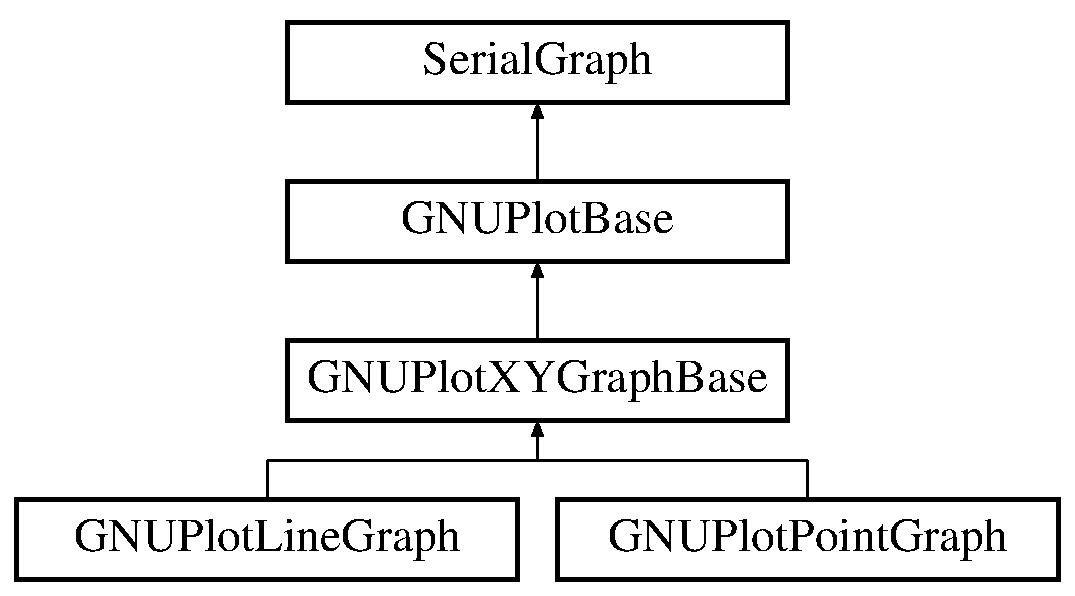
\includegraphics[height=4.000000cm]{class_g_n_u_plot_x_y_graph_base}
\end{center}
\end{figure}
\subsection*{Public Member Functions}
\begin{DoxyCompactItemize}
\item 
\hyperlink{class_g_n_u_plot_x_y_graph_base_a68eed7c5855590fd3b2e696948f071f0}{G\+N\+U\+Plot\+X\+Y\+Graph\+Base} (Print $\ast$\+\_\+out\+Stream)
\item 
virtual \hyperlink{class_g_n_u_plot_x_y_graph_base_a2e03a2909bc036f46aca9b3a86628ada}{$\sim$\+G\+N\+U\+Plot\+X\+Y\+Graph\+Base} ()
\item 
virtual void \hyperlink{class_g_n_u_plot_x_y_graph_base_a8389f830ff330dfb705e00d31053e130}{create\+Graph} ()
\item 
virtual void \hyperlink{class_g_n_u_plot_base_a4d4da234cfdeb99ec3228ef7b2df8a50}{new\+Graph} ()
\item 
virtual void \hyperlink{class_g_n_u_plot_base_aa4b0574c35fbee4dc5f25451eaf956dd}{finish\+Graph} ()
\item 
virtual void \hyperlink{class_g_n_u_plot_base_a219601bd41203477ae73a18d18dd7443}{print\+Comment\+Start} ()
\item 
virtual \hyperlink{_serial_graph_8h_adc73bce6b7e6c4ecf37dde452d6a385e}{Graph\+Style} \hyperlink{class_serial_graph_a2ab97096fffdf429bfa271b9fd4c642a}{get\+Graph\+Style} () const  =0
\item 
virtual void \hyperlink{class_serial_graph_a28b020807c52c113685aa6a31f836c52}{enable\+Save\+Image\+File} (bool enabled)
\item 
virtual void \hyperlink{class_serial_graph_abf488e449d6d786bc01478793d0094ad}{set\+Show\+Grid} (bool enabled)
\item 
void \hyperlink{class_serial_graph_a4db09b008589914b71b2ee8b1873db7a}{set\+Title} (const \+\_\+\+\_\+\+Flash\+String\+Helper $\ast$title)
\item 
virtual void \hyperlink{class_serial_graph_ad726b2c84cec50c2d4bfe769e62a9bcd}{set\+Title} (const char $\ast$title)
\item 
void \hyperlink{class_serial_graph_afdb759a860c41de2fc4cfe78519b9fc0}{set\+X\+Axis\+Name} (const \+\_\+\+\_\+\+Flash\+String\+Helper $\ast$title)
\item 
virtual void \hyperlink{class_serial_graph_ac7f30036f5006091af51204a4d9efaf2}{set\+X\+Axis\+Name} (const char $\ast$name)
\item 
void \hyperlink{class_serial_graph_abfc46c15cf8e1b4362a7f51cb11c7bdb}{set\+Y\+Axis\+Name} (const \+\_\+\+\_\+\+Flash\+String\+Helper $\ast$title)
\item 
virtual void \hyperlink{class_serial_graph_ab0c675c8682959261f79dcf37b04148c}{set\+Y\+Axis\+Name} (const char $\ast$name)
\item 
virtual void \hyperlink{class_serial_graph_ae58de4fa4d391f1a2f411ce00dd74d93}{set\+X\+Axis\+Log} (byte scale)
\item 
virtual void \hyperlink{class_serial_graph_a444e38e8ef3784942ca6ee58940f7023}{set\+Y\+Axis\+Log} (byte scale)
\item 
void \hyperlink{class_serial_graph_a84d8e8ce9bff20e53ba738d1d34d3577}{set\+Series\+Name} (int \+\_\+n, const \+\_\+\+\_\+\+Flash\+String\+Helper $\ast$title)
\item 
virtual void \hyperlink{class_serial_graph_a9d67fbecbee6edb82646aa7ba5103046}{set\+Series\+Name} (int \+\_\+n, const char $\ast$name)
\item 
\hyperlink{struct_line_apperance}{Line\+Apperance} $\ast$ \hyperlink{class_serial_graph_a5a6008dc86a2101a58782929721a5b77}{get\+Line\+Apperance} (int \+\_\+n)
\item 
{\footnotesize template$<$typename Y\+T $>$ }\\void \hyperlink{class_serial_graph_afbcc26bd6bad7179d75379ac0f0d25f1}{plot\+Datum\+Y} (Y\+T y1)
\item 
{\footnotesize template$<$typename X\+T , typename Y\+T $>$ }\\void \hyperlink{class_serial_graph_a265b48fb0afe543e14cedb6619e3931e}{plot\+Datum\+X\+Y} (X\+T x, Y\+T y1)
\item 
{\footnotesize template$<$typename Y\+T $>$ }\\void \hyperlink{class_serial_graph_a56f584fa6316175bc9fbcb4f671f1c93}{plot\+Datum\+Yn} (Y\+T y1, Y\+T y2)
\item 
{\footnotesize template$<$typename Y\+T $>$ }\\void \hyperlink{class_serial_graph_ae755b026606e34c33c4aa8f10d8b5d9c}{plot\+Datum\+Yn} (Y\+T y1, Y\+T y2, Y\+T y3)
\item 
{\footnotesize template$<$typename Y\+T $>$ }\\void \hyperlink{class_serial_graph_a354feb95f91239699d3510c2ce5659b0}{plot\+Datum\+Yn} (Y\+T y1, Y\+T y2, Y\+T y3, Y\+T y4)
\item 
{\footnotesize template$<$typename Y\+T $>$ }\\void \hyperlink{class_serial_graph_ab0fff3fc1879e1cd6aadf24c913ff617}{plot\+Datum\+Yn} (Y\+T y1, Y\+T y2, Y\+T y3, Y\+T y4, Y\+T y5)
\item 
{\footnotesize template$<$typename X\+T , typename Y\+T $>$ }\\void \hyperlink{class_serial_graph_aa20b03efac52c18c50efc79c6459a9fc}{plot\+Datum\+Yn} (const Y\+T $\ast$y\+Vec, int \+\_\+n)
\item 
{\footnotesize template$<$typename X\+T , typename Y\+T $>$ }\\void \hyperlink{class_serial_graph_a79b721ca2be68969862869f96d6a6305}{plot\+Datum\+X\+Yn} (X\+T x, Y\+T y1, Y\+T y2)
\item 
{\footnotesize template$<$typename X\+T , typename Y\+T $>$ }\\void \hyperlink{class_serial_graph_a9fcea879f299a7d24be4ff9a38c53c26}{plot\+Datum\+X\+Yn} (X\+T x, Y\+T y1, Y\+T y2, Y\+T y3)
\item 
{\footnotesize template$<$typename X\+T , typename Y\+T $>$ }\\void \hyperlink{class_serial_graph_afd854b631604abe2014a1bb1beeeec52}{plot\+Datum\+X\+Yn} (X\+T x, Y\+T y1, Y\+T y2, Y\+T y3, Y\+T y4)
\item 
{\footnotesize template$<$typename X\+T , typename Y\+T $>$ }\\void \hyperlink{class_serial_graph_aa1bb6fa08a8bd06c074ac2a02b3f6fbc}{plot\+Datum\+X\+Yn} (X\+T x, Y\+T y1, Y\+T y2, Y\+T y3, Y\+T y4, Y\+T y5)
\item 
{\footnotesize template$<$typename X\+T , typename Y\+T $>$ }\\void \hyperlink{class_serial_graph_a3d7276c89235dc1aa176e2439ad9835b}{plot\+Datum\+X\+Yn} (X\+T x, const Y\+T $\ast$y\+Vec, int \+\_\+n)
\item 
{\footnotesize template$<$typename W\+T $>$ }\\void \hyperlink{class_serial_graph_aa72b48968e82a953dcdc6522bd04c7b4}{print} (const W\+T what)
\item 
{\footnotesize template$<$typename W\+T $>$ }\\void \hyperlink{class_serial_graph_a2005d103cb5a578053ef7838b3a8422d}{println} (const W\+T what)
\item 
{\footnotesize template$<$typename W\+T $>$ }\\void \hyperlink{class_serial_graph_a7237d928f67a14d5c9950d8c23c2a794}{print\+Comment} (const W\+T what)
\item 
{\footnotesize template$<$typename W\+T $>$ }\\void \hyperlink{class_serial_graph_a9b40aa22335fc26a6c29b16d278b26f8}{print\+Comment} (const W\+T $\ast$what)
\end{DoxyCompactItemize}
\subsection*{Public Attributes}
\begin{DoxyCompactItemize}
\item 
const byte \hyperlink{class_serial_graph_a1867ab3a93268646490fa7ba4f8b5680}{max\+String\+Size} = 128
\item 
const byte \hyperlink{class_serial_graph_a752a1429bd35687163fe11c5a2562bef}{max\+Series} = 8
\end{DoxyCompactItemize}
\subsection*{Protected Member Functions}
\begin{DoxyCompactItemize}
\item 
{\footnotesize template$<$typename T , typename U $>$ }\\void \hyperlink{class_g_n_u_plot_base_a03d371b0c6c7ef89064525438b22d52c}{set\+Variable} (T name, U value, bool quoted)
\item 
{\footnotesize template$<$typename T $>$ }\\void \hyperlink{class_g_n_u_plot_base_a3c8c8f68c13661d91bd844589e1a2a85}{set\+Variable} (T name)
\item 
{\footnotesize template$<$typename T $>$ }\\void \hyperlink{class_g_n_u_plot_base_af9b418bbcafb41d4d51b92018ca4f217}{unset\+Variable} (T name)
\item 
{\footnotesize template$<$typename T $>$ }\\void \hyperlink{class_g_n_u_plot_base_a68171bf36461e54e2b81384c112ad975}{set\+Varible\+By\+String\+\_\+null\+Safe} (T name, const char $\ast$text)
\item 
{\footnotesize template$<$typename T $>$ }\\void \hyperlink{class_g_n_u_plot_base_ae93c5de3241c2b6b6f703a202dc1d94b}{set\+Varible\+Flag\+By\+Boolean} (T name, bool value)
\item 
void \hyperlink{class_g_n_u_plot_base_ab5c851953dd140cc3ee936a5cd329200}{save\+Plot\+To\+Image\+File} (const char $\ast$title)
\item 
virtual void \hyperlink{class_g_n_u_plot_base_adaf91c191e4d889537d401faeb863485}{make\+Ready\+For\+Plot\+Data} ()
\item 
char $\ast$ \hyperlink{class_g_n_u_plot_base_a7f71f3c616b3a4a854f9118a04c40447}{malloc\+Basic\+File\+Name\+From\+Graph\+Title} ()
\item 
void \hyperlink{class_g_n_u_plot_base_a65ae2b3220034bce21c7feb39a632991}{print\+Title\+In\+Plot\+Command} (int series\+Num)
\item 
void \hyperlink{class_g_n_u_plot_base_ad057969aa7f8bdbe884d6a5d03a29722}{print\+Line\+Apperance} (\hyperlink{struct_line_apperance}{Line\+Apperance} apperance)
\item 
void \hyperlink{class_g_n_u_plot_base_ad7e8ef8d8e5eb80119fc0cce9be2d525}{print\+Log\+Axis\+Command} (const \+\_\+\+\_\+\+Flash\+String\+Helper $\ast$axis\+Name, byte log\+Scale)
\item 
virtual void \hyperlink{class_g_n_u_plot_base_ae204818b4e8dcd9d2f6b5426127ca2cf}{print\+Seperator} ()
\item 
virtual void \hyperlink{class_g_n_u_plot_base_ac2b48b822b6043392b514c9580b1661a}{print\+Start\+Datum} ()
\item 
virtual void \hyperlink{class_g_n_u_plot_base_aff02bc279e6c3cb83f2cdc7aa021268f}{print\+End\+Datum} ()
\item 
virtual void \hyperlink{class_g_n_u_plot_base_ad00a12fd681e4638fae005891fd72f38}{\+\_\+print\+Data\+Value} (const char $\ast$value)
\item 
virtual void \hyperlink{class_g_n_u_plot_base_aa6c6dfff0568dd99c0c28081c41b4433}{\+\_\+print\+Data\+Value} (char value)
\item 
virtual void \hyperlink{class_g_n_u_plot_base_a6f14fc040ff833c685ab09fc7917e059}{\+\_\+print\+Data\+Value} (bool value)
\item 
virtual void \hyperlink{class_serial_graph_a0c4d2c1239de3107d7332389183b05a1}{\+\_\+print\+Data\+Value} (const \+\_\+\+\_\+\+Flash\+String\+Helper $\ast$value)
\item 
virtual void \hyperlink{class_serial_graph_a58edf4683c600b6bfa1714b0f8dfc82c}{\+\_\+print\+Data\+Value} (int value)
\item 
virtual void \hyperlink{class_serial_graph_a9a4903d4fa26bb85ba5dd93c4365bcc2}{\+\_\+print\+Data\+Value} (long value)
\item 
virtual void \hyperlink{class_serial_graph_acada5333b96b65e31d8c76c3ab22905f}{\+\_\+print\+Data\+Value} (byte value)
\item 
virtual void \hyperlink{class_serial_graph_acd91cf0c3a0f49d4bdf18b447503da23}{\+\_\+print\+Data\+Value} (unsigned int value)
\item 
virtual void \hyperlink{class_serial_graph_a6dbfe61ee398e18c1b752a3748df9663}{\+\_\+print\+Data\+Value} (unsigned long value)
\item 
virtual void \hyperlink{class_serial_graph_a766d5838ede9c8fa998ce8664e5f92be}{\+\_\+print\+Data\+Value} (double value)
\item 
void \hyperlink{class_serial_graph_a760dd00474c9780c81ece7cdf621fc15}{init} ()
\item 
void \hyperlink{class_serial_graph_abd43150abedec26eef3994cd33035173}{ensure\+Ready\+To\+Recive\+Plot\+Data} ()
\item 
{\footnotesize template$<$typename T $>$ }\\void \hyperlink{class_serial_graph_a91e20c05c8cc612fd9ffd85880149264}{print\+Data\+Value} (T value)
\end{DoxyCompactItemize}
\subsection*{Protected Attributes}
\begin{DoxyCompactItemize}
\item 
bool \hyperlink{class_serial_graph_a24202e0a7a8bac5ec1cfd92bf796e078}{save\+File}
\item 
Print $\ast$ \hyperlink{class_serial_graph_aec32289a9393e98bf80d44406e5c207d}{out\+Stream}
\item 
bool \hyperlink{class_serial_graph_a4dbd9cf190c591fb4f2f46a50d937199}{x\+Axis\+Specified}
\item 
int \hyperlink{class_serial_graph_ab40c430e06102b9624736173d4a58596}{num\+Y\+Series}
\item 
bool \hyperlink{class_serial_graph_ad61d5ea29eacc1611c5addc94714f1e2}{show\+Grid}
\item 
char $\ast$ \hyperlink{class_serial_graph_a0b33d43c2bb54340ef1f90b5f76d7aea}{graph\+Title}
\item 
char $\ast$ \hyperlink{class_serial_graph_a5f5bf85ed361ff567d0888eaa73e269c}{x\+Axis\+Name}
\item 
char $\ast$ \hyperlink{class_serial_graph_a08452a56c74ec5f5473b64605d555339}{y\+Axis\+Name}
\item 
char $\ast$$\ast$ \hyperlink{class_serial_graph_a2307e40e27249f44bbe14776dc68c561}{series\+Names}
\item 
\hyperlink{struct_line_apperance}{Line\+Apperance} $\ast$ \hyperlink{class_serial_graph_a8d743f9eeeca69a988d2159a405e4253}{series\+Apperance}
\item 
byte \hyperlink{class_serial_graph_afc2ca72fdfe2bc5e3159c9e910a8f81e}{x\+Axis\+Log\+Scale}
\item 
byte \hyperlink{class_serial_graph_a1f0424857ec14c176747b3ddb0768eee}{y\+Axis\+Log\+Scale}
\end{DoxyCompactItemize}


\subsection{Detailed Description}
A base class for all line and point plots. 

\subsection{Constructor \& Destructor Documentation}
\hypertarget{class_g_n_u_plot_x_y_graph_base_a68eed7c5855590fd3b2e696948f071f0}{}\index{G\+N\+U\+Plot\+X\+Y\+Graph\+Base@{G\+N\+U\+Plot\+X\+Y\+Graph\+Base}!G\+N\+U\+Plot\+X\+Y\+Graph\+Base@{G\+N\+U\+Plot\+X\+Y\+Graph\+Base}}
\index{G\+N\+U\+Plot\+X\+Y\+Graph\+Base@{G\+N\+U\+Plot\+X\+Y\+Graph\+Base}!G\+N\+U\+Plot\+X\+Y\+Graph\+Base@{G\+N\+U\+Plot\+X\+Y\+Graph\+Base}}
\subsubsection[{G\+N\+U\+Plot\+X\+Y\+Graph\+Base(\+Print $\ast$\+\_\+out\+Stream)}]{\setlength{\rightskip}{0pt plus 5cm}G\+N\+U\+Plot\+X\+Y\+Graph\+Base\+::\+G\+N\+U\+Plot\+X\+Y\+Graph\+Base (
\begin{DoxyParamCaption}
\item[{Print $\ast$}]{\+\_\+out\+Stream}
\end{DoxyParamCaption}
)\hspace{0.3cm}{\ttfamily [inline]}}\label{class_g_n_u_plot_x_y_graph_base_a68eed7c5855590fd3b2e696948f071f0}
\hypertarget{class_g_n_u_plot_x_y_graph_base_a2e03a2909bc036f46aca9b3a86628ada}{}\index{G\+N\+U\+Plot\+X\+Y\+Graph\+Base@{G\+N\+U\+Plot\+X\+Y\+Graph\+Base}!````~G\+N\+U\+Plot\+X\+Y\+Graph\+Base@{$\sim$\+G\+N\+U\+Plot\+X\+Y\+Graph\+Base}}
\index{````~G\+N\+U\+Plot\+X\+Y\+Graph\+Base@{$\sim$\+G\+N\+U\+Plot\+X\+Y\+Graph\+Base}!G\+N\+U\+Plot\+X\+Y\+Graph\+Base@{G\+N\+U\+Plot\+X\+Y\+Graph\+Base}}
\subsubsection[{$\sim$\+G\+N\+U\+Plot\+X\+Y\+Graph\+Base()}]{\setlength{\rightskip}{0pt plus 5cm}virtual G\+N\+U\+Plot\+X\+Y\+Graph\+Base\+::$\sim$\+G\+N\+U\+Plot\+X\+Y\+Graph\+Base (
\begin{DoxyParamCaption}
{}
\end{DoxyParamCaption}
)\hspace{0.3cm}{\ttfamily [inline]}, {\ttfamily [virtual]}}\label{class_g_n_u_plot_x_y_graph_base_a2e03a2909bc036f46aca9b3a86628ada}


\subsection{Member Function Documentation}
\hypertarget{class_g_n_u_plot_base_ad00a12fd681e4638fae005891fd72f38}{}\index{G\+N\+U\+Plot\+X\+Y\+Graph\+Base@{G\+N\+U\+Plot\+X\+Y\+Graph\+Base}!\+\_\+print\+Data\+Value@{\+\_\+print\+Data\+Value}}
\index{\+\_\+print\+Data\+Value@{\+\_\+print\+Data\+Value}!G\+N\+U\+Plot\+X\+Y\+Graph\+Base@{G\+N\+U\+Plot\+X\+Y\+Graph\+Base}}
\subsubsection[{\+\_\+print\+Data\+Value(const char $\ast$value)}]{\setlength{\rightskip}{0pt plus 5cm}void G\+N\+U\+Plot\+Base\+::\+\_\+print\+Data\+Value (
\begin{DoxyParamCaption}
\item[{const char $\ast$}]{value}
\end{DoxyParamCaption}
)\hspace{0.3cm}{\ttfamily [protected]}, {\ttfamily [virtual]}, {\ttfamily [inherited]}}\label{class_g_n_u_plot_base_ad00a12fd681e4638fae005891fd72f38}
Override a put appropriate quotes around strings etc. 
\begin{DoxyParams}{Parameters}
{\em value} & What to print. \\
\hline
\end{DoxyParams}


Reimplemented from \hyperlink{class_serial_graph_a8252997dd4bad0251d437d6dd097bffb}{Serial\+Graph}.

\hypertarget{class_g_n_u_plot_base_aa6c6dfff0568dd99c0c28081c41b4433}{}\index{G\+N\+U\+Plot\+X\+Y\+Graph\+Base@{G\+N\+U\+Plot\+X\+Y\+Graph\+Base}!\+\_\+print\+Data\+Value@{\+\_\+print\+Data\+Value}}
\index{\+\_\+print\+Data\+Value@{\+\_\+print\+Data\+Value}!G\+N\+U\+Plot\+X\+Y\+Graph\+Base@{G\+N\+U\+Plot\+X\+Y\+Graph\+Base}}
\subsubsection[{\+\_\+print\+Data\+Value(char value)}]{\setlength{\rightskip}{0pt plus 5cm}virtual void G\+N\+U\+Plot\+Base\+::\+\_\+print\+Data\+Value (
\begin{DoxyParamCaption}
\item[{char}]{value}
\end{DoxyParamCaption}
)\hspace{0.3cm}{\ttfamily [inline]}, {\ttfamily [protected]}, {\ttfamily [virtual]}, {\ttfamily [inherited]}}\label{class_g_n_u_plot_base_aa6c6dfff0568dd99c0c28081c41b4433}
Override for customised value output. 
\begin{DoxyParams}{Parameters}
{\em value} & What to print. \\
\hline
\end{DoxyParams}


Reimplemented from \hyperlink{class_serial_graph_af3fbf7a9201f71cd6bad7e4337092fb6}{Serial\+Graph}.

\hypertarget{class_g_n_u_plot_base_a6f14fc040ff833c685ab09fc7917e059}{}\index{G\+N\+U\+Plot\+X\+Y\+Graph\+Base@{G\+N\+U\+Plot\+X\+Y\+Graph\+Base}!\+\_\+print\+Data\+Value@{\+\_\+print\+Data\+Value}}
\index{\+\_\+print\+Data\+Value@{\+\_\+print\+Data\+Value}!G\+N\+U\+Plot\+X\+Y\+Graph\+Base@{G\+N\+U\+Plot\+X\+Y\+Graph\+Base}}
\subsubsection[{\+\_\+print\+Data\+Value(bool value)}]{\setlength{\rightskip}{0pt plus 5cm}virtual void G\+N\+U\+Plot\+Base\+::\+\_\+print\+Data\+Value (
\begin{DoxyParamCaption}
\item[{bool}]{value}
\end{DoxyParamCaption}
)\hspace{0.3cm}{\ttfamily [inline]}, {\ttfamily [protected]}, {\ttfamily [virtual]}, {\ttfamily [inherited]}}\label{class_g_n_u_plot_base_a6f14fc040ff833c685ab09fc7917e059}
Override for customised value output. 
\begin{DoxyParams}{Parameters}
{\em value} & What to print. \\
\hline
\end{DoxyParams}


Reimplemented from \hyperlink{class_serial_graph_aed9ff95634ace3d190863ea9d15c10da}{Serial\+Graph}.

\hypertarget{class_serial_graph_a0c4d2c1239de3107d7332389183b05a1}{}\index{G\+N\+U\+Plot\+X\+Y\+Graph\+Base@{G\+N\+U\+Plot\+X\+Y\+Graph\+Base}!\+\_\+print\+Data\+Value@{\+\_\+print\+Data\+Value}}
\index{\+\_\+print\+Data\+Value@{\+\_\+print\+Data\+Value}!G\+N\+U\+Plot\+X\+Y\+Graph\+Base@{G\+N\+U\+Plot\+X\+Y\+Graph\+Base}}
\subsubsection[{\+\_\+print\+Data\+Value(const \+\_\+\+\_\+\+Flash\+String\+Helper $\ast$value)}]{\setlength{\rightskip}{0pt plus 5cm}virtual void Serial\+Graph\+::\+\_\+print\+Data\+Value (
\begin{DoxyParamCaption}
\item[{const \+\_\+\+\_\+\+Flash\+String\+Helper $\ast$}]{value}
\end{DoxyParamCaption}
)\hspace{0.3cm}{\ttfamily [inline]}, {\ttfamily [protected]}, {\ttfamily [virtual]}, {\ttfamily [inherited]}}\label{class_serial_graph_a0c4d2c1239de3107d7332389183b05a1}
This just calls \hyperlink{class_serial_graph_a8252997dd4bad0251d437d6dd097bffb}{\+\_\+print\+Data\+Value(const char $\ast$value)} so probably alter that instead. 
\begin{DoxyParams}{Parameters}
{\em value} & What to print. \\
\hline
\end{DoxyParams}
\hypertarget{class_serial_graph_a58edf4683c600b6bfa1714b0f8dfc82c}{}\index{G\+N\+U\+Plot\+X\+Y\+Graph\+Base@{G\+N\+U\+Plot\+X\+Y\+Graph\+Base}!\+\_\+print\+Data\+Value@{\+\_\+print\+Data\+Value}}
\index{\+\_\+print\+Data\+Value@{\+\_\+print\+Data\+Value}!G\+N\+U\+Plot\+X\+Y\+Graph\+Base@{G\+N\+U\+Plot\+X\+Y\+Graph\+Base}}
\subsubsection[{\+\_\+print\+Data\+Value(int value)}]{\setlength{\rightskip}{0pt plus 5cm}virtual void Serial\+Graph\+::\+\_\+print\+Data\+Value (
\begin{DoxyParamCaption}
\item[{int}]{value}
\end{DoxyParamCaption}
)\hspace{0.3cm}{\ttfamily [inline]}, {\ttfamily [protected]}, {\ttfamily [virtual]}, {\ttfamily [inherited]}}\label{class_serial_graph_a58edf4683c600b6bfa1714b0f8dfc82c}
Override for customised value output. 
\begin{DoxyParams}{Parameters}
{\em value} & What to print. \\
\hline
\end{DoxyParams}
\hypertarget{class_serial_graph_a9a4903d4fa26bb85ba5dd93c4365bcc2}{}\index{G\+N\+U\+Plot\+X\+Y\+Graph\+Base@{G\+N\+U\+Plot\+X\+Y\+Graph\+Base}!\+\_\+print\+Data\+Value@{\+\_\+print\+Data\+Value}}
\index{\+\_\+print\+Data\+Value@{\+\_\+print\+Data\+Value}!G\+N\+U\+Plot\+X\+Y\+Graph\+Base@{G\+N\+U\+Plot\+X\+Y\+Graph\+Base}}
\subsubsection[{\+\_\+print\+Data\+Value(long value)}]{\setlength{\rightskip}{0pt plus 5cm}virtual void Serial\+Graph\+::\+\_\+print\+Data\+Value (
\begin{DoxyParamCaption}
\item[{long}]{value}
\end{DoxyParamCaption}
)\hspace{0.3cm}{\ttfamily [inline]}, {\ttfamily [protected]}, {\ttfamily [virtual]}, {\ttfamily [inherited]}}\label{class_serial_graph_a9a4903d4fa26bb85ba5dd93c4365bcc2}
Override for customised value output. 
\begin{DoxyParams}{Parameters}
{\em value} & What to print. \\
\hline
\end{DoxyParams}
\hypertarget{class_serial_graph_acada5333b96b65e31d8c76c3ab22905f}{}\index{G\+N\+U\+Plot\+X\+Y\+Graph\+Base@{G\+N\+U\+Plot\+X\+Y\+Graph\+Base}!\+\_\+print\+Data\+Value@{\+\_\+print\+Data\+Value}}
\index{\+\_\+print\+Data\+Value@{\+\_\+print\+Data\+Value}!G\+N\+U\+Plot\+X\+Y\+Graph\+Base@{G\+N\+U\+Plot\+X\+Y\+Graph\+Base}}
\subsubsection[{\+\_\+print\+Data\+Value(byte value)}]{\setlength{\rightskip}{0pt plus 5cm}virtual void Serial\+Graph\+::\+\_\+print\+Data\+Value (
\begin{DoxyParamCaption}
\item[{byte}]{value}
\end{DoxyParamCaption}
)\hspace{0.3cm}{\ttfamily [inline]}, {\ttfamily [protected]}, {\ttfamily [virtual]}, {\ttfamily [inherited]}}\label{class_serial_graph_acada5333b96b65e31d8c76c3ab22905f}
Override for customised value output. 
\begin{DoxyParams}{Parameters}
{\em value} & What to print. \\
\hline
\end{DoxyParams}
\hypertarget{class_serial_graph_acd91cf0c3a0f49d4bdf18b447503da23}{}\index{G\+N\+U\+Plot\+X\+Y\+Graph\+Base@{G\+N\+U\+Plot\+X\+Y\+Graph\+Base}!\+\_\+print\+Data\+Value@{\+\_\+print\+Data\+Value}}
\index{\+\_\+print\+Data\+Value@{\+\_\+print\+Data\+Value}!G\+N\+U\+Plot\+X\+Y\+Graph\+Base@{G\+N\+U\+Plot\+X\+Y\+Graph\+Base}}
\subsubsection[{\+\_\+print\+Data\+Value(unsigned int value)}]{\setlength{\rightskip}{0pt plus 5cm}virtual void Serial\+Graph\+::\+\_\+print\+Data\+Value (
\begin{DoxyParamCaption}
\item[{unsigned int}]{value}
\end{DoxyParamCaption}
)\hspace{0.3cm}{\ttfamily [inline]}, {\ttfamily [protected]}, {\ttfamily [virtual]}, {\ttfamily [inherited]}}\label{class_serial_graph_acd91cf0c3a0f49d4bdf18b447503da23}
Override for customised value output. 
\begin{DoxyParams}{Parameters}
{\em value} & What to print. \\
\hline
\end{DoxyParams}
\hypertarget{class_serial_graph_a6dbfe61ee398e18c1b752a3748df9663}{}\index{G\+N\+U\+Plot\+X\+Y\+Graph\+Base@{G\+N\+U\+Plot\+X\+Y\+Graph\+Base}!\+\_\+print\+Data\+Value@{\+\_\+print\+Data\+Value}}
\index{\+\_\+print\+Data\+Value@{\+\_\+print\+Data\+Value}!G\+N\+U\+Plot\+X\+Y\+Graph\+Base@{G\+N\+U\+Plot\+X\+Y\+Graph\+Base}}
\subsubsection[{\+\_\+print\+Data\+Value(unsigned long value)}]{\setlength{\rightskip}{0pt plus 5cm}virtual void Serial\+Graph\+::\+\_\+print\+Data\+Value (
\begin{DoxyParamCaption}
\item[{unsigned long}]{value}
\end{DoxyParamCaption}
)\hspace{0.3cm}{\ttfamily [inline]}, {\ttfamily [protected]}, {\ttfamily [virtual]}, {\ttfamily [inherited]}}\label{class_serial_graph_a6dbfe61ee398e18c1b752a3748df9663}
Override for customised value output. 
\begin{DoxyParams}{Parameters}
{\em value} & What to print. \\
\hline
\end{DoxyParams}
\hypertarget{class_serial_graph_a766d5838ede9c8fa998ce8664e5f92be}{}\index{G\+N\+U\+Plot\+X\+Y\+Graph\+Base@{G\+N\+U\+Plot\+X\+Y\+Graph\+Base}!\+\_\+print\+Data\+Value@{\+\_\+print\+Data\+Value}}
\index{\+\_\+print\+Data\+Value@{\+\_\+print\+Data\+Value}!G\+N\+U\+Plot\+X\+Y\+Graph\+Base@{G\+N\+U\+Plot\+X\+Y\+Graph\+Base}}
\subsubsection[{\+\_\+print\+Data\+Value(double value)}]{\setlength{\rightskip}{0pt plus 5cm}virtual void Serial\+Graph\+::\+\_\+print\+Data\+Value (
\begin{DoxyParamCaption}
\item[{double}]{value}
\end{DoxyParamCaption}
)\hspace{0.3cm}{\ttfamily [inline]}, {\ttfamily [protected]}, {\ttfamily [virtual]}, {\ttfamily [inherited]}}\label{class_serial_graph_a766d5838ede9c8fa998ce8664e5f92be}
Override for customised value output. 
\begin{DoxyParams}{Parameters}
{\em value} & What to print. \\
\hline
\end{DoxyParams}
\hypertarget{class_g_n_u_plot_x_y_graph_base_a8389f830ff330dfb705e00d31053e130}{}\index{G\+N\+U\+Plot\+X\+Y\+Graph\+Base@{G\+N\+U\+Plot\+X\+Y\+Graph\+Base}!create\+Graph@{create\+Graph}}
\index{create\+Graph@{create\+Graph}!G\+N\+U\+Plot\+X\+Y\+Graph\+Base@{G\+N\+U\+Plot\+X\+Y\+Graph\+Base}}
\subsubsection[{create\+Graph()}]{\setlength{\rightskip}{0pt plus 5cm}void G\+N\+U\+Plot\+X\+Y\+Graph\+Base\+::create\+Graph (
\begin{DoxyParamCaption}
{}
\end{DoxyParamCaption}
)\hspace{0.3cm}{\ttfamily [virtual]}}\label{class_g_n_u_plot_x_y_graph_base_a8389f830ff330dfb705e00d31053e130}


Implements \hyperlink{class_g_n_u_plot_base_ad877f207d43e6f9cd0aa0ef241e31c24}{G\+N\+U\+Plot\+Base}.

\hypertarget{class_serial_graph_a28b020807c52c113685aa6a31f836c52}{}\index{G\+N\+U\+Plot\+X\+Y\+Graph\+Base@{G\+N\+U\+Plot\+X\+Y\+Graph\+Base}!enable\+Save\+Image\+File@{enable\+Save\+Image\+File}}
\index{enable\+Save\+Image\+File@{enable\+Save\+Image\+File}!G\+N\+U\+Plot\+X\+Y\+Graph\+Base@{G\+N\+U\+Plot\+X\+Y\+Graph\+Base}}
\subsubsection[{enable\+Save\+Image\+File(bool enabled)}]{\setlength{\rightskip}{0pt plus 5cm}virtual void Serial\+Graph\+::enable\+Save\+Image\+File (
\begin{DoxyParamCaption}
\item[{bool}]{enabled}
\end{DoxyParamCaption}
)\hspace{0.3cm}{\ttfamily [inline]}, {\ttfamily [virtual]}, {\ttfamily [inherited]}}\label{class_serial_graph_a28b020807c52c113685aa6a31f836c52}
Set to true if an image file should be saved. \begin{DoxyNote}{Note}
Filename will be based on graph title. This is done to save memory. Final filename has some extra validation performed to conform with filename rules aplicable to modern operating systems (excluding 8 char limit). 
\end{DoxyNote}
\hypertarget{class_serial_graph_abd43150abedec26eef3994cd33035173}{}\index{G\+N\+U\+Plot\+X\+Y\+Graph\+Base@{G\+N\+U\+Plot\+X\+Y\+Graph\+Base}!ensure\+Ready\+To\+Recive\+Plot\+Data@{ensure\+Ready\+To\+Recive\+Plot\+Data}}
\index{ensure\+Ready\+To\+Recive\+Plot\+Data@{ensure\+Ready\+To\+Recive\+Plot\+Data}!G\+N\+U\+Plot\+X\+Y\+Graph\+Base@{G\+N\+U\+Plot\+X\+Y\+Graph\+Base}}
\subsubsection[{ensure\+Ready\+To\+Recive\+Plot\+Data()}]{\setlength{\rightskip}{0pt plus 5cm}void Serial\+Graph\+::ensure\+Ready\+To\+Recive\+Plot\+Data (
\begin{DoxyParamCaption}
{}
\end{DoxyParamCaption}
)\hspace{0.3cm}{\ttfamily [protected]}, {\ttfamily [inherited]}}\label{class_serial_graph_abd43150abedec26eef3994cd33035173}
Called by every plot command prior to sending data. it\textquotesingle{}s function is to call \hyperlink{class_serial_graph_a898cf274c886e0ff45e90d3f21f0a6cc}{make\+Ready\+For\+Plot\+Data()} the first time it is called. 
\begin{DoxyParams}{Parameters}
{\em value} & What to print. \\
\hline
\end{DoxyParams}
\hypertarget{class_g_n_u_plot_base_aa4b0574c35fbee4dc5f25451eaf956dd}{}\index{G\+N\+U\+Plot\+X\+Y\+Graph\+Base@{G\+N\+U\+Plot\+X\+Y\+Graph\+Base}!finish\+Graph@{finish\+Graph}}
\index{finish\+Graph@{finish\+Graph}!G\+N\+U\+Plot\+X\+Y\+Graph\+Base@{G\+N\+U\+Plot\+X\+Y\+Graph\+Base}}
\subsubsection[{finish\+Graph()}]{\setlength{\rightskip}{0pt plus 5cm}void G\+N\+U\+Plot\+Base\+::finish\+Graph (
\begin{DoxyParamCaption}
{}
\end{DoxyParamCaption}
)\hspace{0.3cm}{\ttfamily [virtual]}, {\ttfamily [inherited]}}\label{class_g_n_u_plot_base_aa4b0574c35fbee4dc5f25451eaf956dd}
Serial output that finishes the plot, saves file, updates display etc. 

Implements \hyperlink{class_serial_graph_a8054ce989a1788bd35d2fde56081c88c}{Serial\+Graph}.

\hypertarget{class_serial_graph_a2ab97096fffdf429bfa271b9fd4c642a}{}\index{G\+N\+U\+Plot\+X\+Y\+Graph\+Base@{G\+N\+U\+Plot\+X\+Y\+Graph\+Base}!get\+Graph\+Style@{get\+Graph\+Style}}
\index{get\+Graph\+Style@{get\+Graph\+Style}!G\+N\+U\+Plot\+X\+Y\+Graph\+Base@{G\+N\+U\+Plot\+X\+Y\+Graph\+Base}}
\subsubsection[{get\+Graph\+Style() const  =0}]{\setlength{\rightskip}{0pt plus 5cm}virtual {\bf Graph\+Style} Serial\+Graph\+::get\+Graph\+Style (
\begin{DoxyParamCaption}
{}
\end{DoxyParamCaption}
) const\hspace{0.3cm}{\ttfamily [pure virtual]}, {\ttfamily [inherited]}}\label{class_serial_graph_a2ab97096fffdf429bfa271b9fd4c642a}
Returns the Graph\+Style of the current object. 

Implemented in \hyperlink{class_g_n_u_plot_bar_graph_a6b2cde2832fcb246361d8ebddbe7a228}{G\+N\+U\+Plot\+Bar\+Graph}, \hyperlink{class_g_n_u_plot_point_graph_aeeae395426112202d3617ff66d836c99}{G\+N\+U\+Plot\+Point\+Graph}, and \hyperlink{class_g_n_u_plot_line_graph_a8f8b19efd8d8f4f25ccc41635e332593}{G\+N\+U\+Plot\+Line\+Graph}.

\hypertarget{class_serial_graph_a5a6008dc86a2101a58782929721a5b77}{}\index{G\+N\+U\+Plot\+X\+Y\+Graph\+Base@{G\+N\+U\+Plot\+X\+Y\+Graph\+Base}!get\+Line\+Apperance@{get\+Line\+Apperance}}
\index{get\+Line\+Apperance@{get\+Line\+Apperance}!G\+N\+U\+Plot\+X\+Y\+Graph\+Base@{G\+N\+U\+Plot\+X\+Y\+Graph\+Base}}
\subsubsection[{get\+Line\+Apperance(int \+\_\+n)}]{\setlength{\rightskip}{0pt plus 5cm}{\bf Line\+Apperance}$\ast$ Serial\+Graph\+::get\+Line\+Apperance (
\begin{DoxyParamCaption}
\item[{int}]{\+\_\+n}
\end{DoxyParamCaption}
)\hspace{0.3cm}{\ttfamily [inline]}, {\ttfamily [inherited]}}\label{class_serial_graph_a5a6008dc86a2101a58782929721a5b77}
Gets a structure that controls apperance of a series (called a \hyperlink{struct_line_apperance}{Line\+Apperance}). It is intended that you directly modify the structure returned, there is no set\+Line\+Apperance. See the struct \hyperlink{struct_line_apperance}{Line\+Apperance} for more.


\begin{DoxyParams}{Parameters}
{\em \+\_\+n} & Series number to alter.\\
\hline
\end{DoxyParams}
\begin{DoxyNote}{Note}
Behaviour on \+\_\+n $>$ max\+Series, is to just override the last possible series entry. 
\end{DoxyNote}
\hypertarget{class_serial_graph_a760dd00474c9780c81ece7cdf621fc15}{}\index{G\+N\+U\+Plot\+X\+Y\+Graph\+Base@{G\+N\+U\+Plot\+X\+Y\+Graph\+Base}!init@{init}}
\index{init@{init}!G\+N\+U\+Plot\+X\+Y\+Graph\+Base@{G\+N\+U\+Plot\+X\+Y\+Graph\+Base}}
\subsubsection[{init()}]{\setlength{\rightskip}{0pt plus 5cm}void Serial\+Graph\+::init (
\begin{DoxyParamCaption}
{}
\end{DoxyParamCaption}
)\hspace{0.3cm}{\ttfamily [protected]}, {\ttfamily [inherited]}}\label{class_serial_graph_a760dd00474c9780c81ece7cdf621fc15}
Brings the class to its default state. Called by the constructor and \hyperlink{class_serial_graph_a44d34593c56aa67142ccd9fcc0a1da86}{new\+Graph()}. \hypertarget{class_g_n_u_plot_base_adaf91c191e4d889537d401faeb863485}{}\index{G\+N\+U\+Plot\+X\+Y\+Graph\+Base@{G\+N\+U\+Plot\+X\+Y\+Graph\+Base}!make\+Ready\+For\+Plot\+Data@{make\+Ready\+For\+Plot\+Data}}
\index{make\+Ready\+For\+Plot\+Data@{make\+Ready\+For\+Plot\+Data}!G\+N\+U\+Plot\+X\+Y\+Graph\+Base@{G\+N\+U\+Plot\+X\+Y\+Graph\+Base}}
\subsubsection[{make\+Ready\+For\+Plot\+Data()}]{\setlength{\rightskip}{0pt plus 5cm}void G\+N\+U\+Plot\+Base\+::make\+Ready\+For\+Plot\+Data (
\begin{DoxyParamCaption}
{}
\end{DoxyParamCaption}
)\hspace{0.3cm}{\ttfamily [protected]}, {\ttfamily [virtual]}, {\ttfamily [inherited]}}\label{class_g_n_u_plot_base_adaf91c191e4d889537d401faeb863485}
Called by ensure\+Ready\+To\+Recive\+Plot\+Data, if the first plot command is encountered. \begin{DoxyNote}{Note}
A concrete class should override this. 
\end{DoxyNote}


Reimplemented from \hyperlink{class_serial_graph_a898cf274c886e0ff45e90d3f21f0a6cc}{Serial\+Graph}.

\hypertarget{class_g_n_u_plot_base_a7f71f3c616b3a4a854f9118a04c40447}{}\index{G\+N\+U\+Plot\+X\+Y\+Graph\+Base@{G\+N\+U\+Plot\+X\+Y\+Graph\+Base}!malloc\+Basic\+File\+Name\+From\+Graph\+Title@{malloc\+Basic\+File\+Name\+From\+Graph\+Title}}
\index{malloc\+Basic\+File\+Name\+From\+Graph\+Title@{malloc\+Basic\+File\+Name\+From\+Graph\+Title}!G\+N\+U\+Plot\+X\+Y\+Graph\+Base@{G\+N\+U\+Plot\+X\+Y\+Graph\+Base}}
\subsubsection[{malloc\+Basic\+File\+Name\+From\+Graph\+Title()}]{\setlength{\rightskip}{0pt plus 5cm}char $\ast$ G\+N\+U\+Plot\+Base\+::malloc\+Basic\+File\+Name\+From\+Graph\+Title (
\begin{DoxyParamCaption}
{}
\end{DoxyParamCaption}
)\hspace{0.3cm}{\ttfamily [protected]}, {\ttfamily [inherited]}}\label{class_g_n_u_plot_base_a7f71f3c616b3a4a854f9118a04c40447}
\hypertarget{class_g_n_u_plot_base_a4d4da234cfdeb99ec3228ef7b2df8a50}{}\index{G\+N\+U\+Plot\+X\+Y\+Graph\+Base@{G\+N\+U\+Plot\+X\+Y\+Graph\+Base}!new\+Graph@{new\+Graph}}
\index{new\+Graph@{new\+Graph}!G\+N\+U\+Plot\+X\+Y\+Graph\+Base@{G\+N\+U\+Plot\+X\+Y\+Graph\+Base}}
\subsubsection[{new\+Graph()}]{\setlength{\rightskip}{0pt plus 5cm}void G\+N\+U\+Plot\+Base\+::new\+Graph (
\begin{DoxyParamCaption}
{}
\end{DoxyParamCaption}
)\hspace{0.3cm}{\ttfamily [virtual]}, {\ttfamily [inherited]}}\label{class_g_n_u_plot_base_a4d4da234cfdeb99ec3228ef7b2df8a50}
Serial output that establishes a new graph. This should also call \hyperlink{class_serial_graph_a760dd00474c9780c81ece7cdf621fc15}{init()}, to reset the class. \begin{DoxyNote}{Note}
\+: If you wan\textquotesingle{}t a \char`\"{}memory breather\char`\"{} between plots, calling this method frees all series names, titles etc. 
\end{DoxyNote}


Implements \hyperlink{class_serial_graph_a44d34593c56aa67142ccd9fcc0a1da86}{Serial\+Graph}.

\hypertarget{class_serial_graph_a265b48fb0afe543e14cedb6619e3931e}{}\index{G\+N\+U\+Plot\+X\+Y\+Graph\+Base@{G\+N\+U\+Plot\+X\+Y\+Graph\+Base}!plot\+Datum\+X\+Y@{plot\+Datum\+X\+Y}}
\index{plot\+Datum\+X\+Y@{plot\+Datum\+X\+Y}!G\+N\+U\+Plot\+X\+Y\+Graph\+Base@{G\+N\+U\+Plot\+X\+Y\+Graph\+Base}}
\subsubsection[{plot\+Datum\+X\+Y(\+X\+T x, Y\+T y1)}]{\setlength{\rightskip}{0pt plus 5cm}template$<$typename X\+T , typename Y\+T $>$ void Serial\+Graph\+::plot\+Datum\+X\+Y (
\begin{DoxyParamCaption}
\item[{X\+T}]{x, }
\item[{Y\+T}]{y1}
\end{DoxyParamCaption}
)\hspace{0.3cm}{\ttfamily [inline]}, {\ttfamily [inherited]}}\label{class_serial_graph_a265b48fb0afe543e14cedb6619e3931e}
Outputs a point to be plotted. All Y values must be of the same type.

\begin{DoxyNote}{Note}
The first time this is called after \hyperlink{class_serial_graph_a44d34593c56aa67142ccd9fcc0a1da86}{new\+Graph()}, \hyperlink{class_serial_graph_a898cf274c886e0ff45e90d3f21f0a6cc}{make\+Ready\+For\+Plot\+Data()} will be called. 

The following feilds automatically set\+: x\+Axis\+Specified; num\+Y\+Series; 
\end{DoxyNote}
\hypertarget{class_serial_graph_a79b721ca2be68969862869f96d6a6305}{}\index{G\+N\+U\+Plot\+X\+Y\+Graph\+Base@{G\+N\+U\+Plot\+X\+Y\+Graph\+Base}!plot\+Datum\+X\+Yn@{plot\+Datum\+X\+Yn}}
\index{plot\+Datum\+X\+Yn@{plot\+Datum\+X\+Yn}!G\+N\+U\+Plot\+X\+Y\+Graph\+Base@{G\+N\+U\+Plot\+X\+Y\+Graph\+Base}}
\subsubsection[{plot\+Datum\+X\+Yn(\+X\+T x, Y\+T y1, Y\+T y2)}]{\setlength{\rightskip}{0pt plus 5cm}template$<$typename X\+T , typename Y\+T $>$ void Serial\+Graph\+::plot\+Datum\+X\+Yn (
\begin{DoxyParamCaption}
\item[{X\+T}]{x, }
\item[{Y\+T}]{y1, }
\item[{Y\+T}]{y2}
\end{DoxyParamCaption}
)\hspace{0.3cm}{\ttfamily [inline]}, {\ttfamily [inherited]}}\label{class_serial_graph_a79b721ca2be68969862869f96d6a6305}
Outputs a point to be plotted. All Y values must be of the same type.

\begin{DoxyNote}{Note}
The first time this is called after \hyperlink{class_serial_graph_a44d34593c56aa67142ccd9fcc0a1da86}{new\+Graph()}, \hyperlink{class_serial_graph_a898cf274c886e0ff45e90d3f21f0a6cc}{make\+Ready\+For\+Plot\+Data()} will be called. 

The following feilds automatically set\+: x\+Axis\+Specified; num\+Y\+Series; 
\end{DoxyNote}
\hypertarget{class_serial_graph_a9fcea879f299a7d24be4ff9a38c53c26}{}\index{G\+N\+U\+Plot\+X\+Y\+Graph\+Base@{G\+N\+U\+Plot\+X\+Y\+Graph\+Base}!plot\+Datum\+X\+Yn@{plot\+Datum\+X\+Yn}}
\index{plot\+Datum\+X\+Yn@{plot\+Datum\+X\+Yn}!G\+N\+U\+Plot\+X\+Y\+Graph\+Base@{G\+N\+U\+Plot\+X\+Y\+Graph\+Base}}
\subsubsection[{plot\+Datum\+X\+Yn(\+X\+T x, Y\+T y1, Y\+T y2, Y\+T y3)}]{\setlength{\rightskip}{0pt plus 5cm}template$<$typename X\+T , typename Y\+T $>$ void Serial\+Graph\+::plot\+Datum\+X\+Yn (
\begin{DoxyParamCaption}
\item[{X\+T}]{x, }
\item[{Y\+T}]{y1, }
\item[{Y\+T}]{y2, }
\item[{Y\+T}]{y3}
\end{DoxyParamCaption}
)\hspace{0.3cm}{\ttfamily [inline]}, {\ttfamily [inherited]}}\label{class_serial_graph_a9fcea879f299a7d24be4ff9a38c53c26}
Outputs a point to be plotted. All Y values must be of the same type.

\begin{DoxyNote}{Note}
The first time this is called after \hyperlink{class_serial_graph_a44d34593c56aa67142ccd9fcc0a1da86}{new\+Graph()}, \hyperlink{class_serial_graph_a898cf274c886e0ff45e90d3f21f0a6cc}{make\+Ready\+For\+Plot\+Data()} will be called. 

The following feilds automatically set\+: x\+Axis\+Specified; num\+Y\+Series; 
\end{DoxyNote}
\hypertarget{class_serial_graph_afd854b631604abe2014a1bb1beeeec52}{}\index{G\+N\+U\+Plot\+X\+Y\+Graph\+Base@{G\+N\+U\+Plot\+X\+Y\+Graph\+Base}!plot\+Datum\+X\+Yn@{plot\+Datum\+X\+Yn}}
\index{plot\+Datum\+X\+Yn@{plot\+Datum\+X\+Yn}!G\+N\+U\+Plot\+X\+Y\+Graph\+Base@{G\+N\+U\+Plot\+X\+Y\+Graph\+Base}}
\subsubsection[{plot\+Datum\+X\+Yn(\+X\+T x, Y\+T y1, Y\+T y2, Y\+T y3, Y\+T y4)}]{\setlength{\rightskip}{0pt plus 5cm}template$<$typename X\+T , typename Y\+T $>$ void Serial\+Graph\+::plot\+Datum\+X\+Yn (
\begin{DoxyParamCaption}
\item[{X\+T}]{x, }
\item[{Y\+T}]{y1, }
\item[{Y\+T}]{y2, }
\item[{Y\+T}]{y3, }
\item[{Y\+T}]{y4}
\end{DoxyParamCaption}
)\hspace{0.3cm}{\ttfamily [inline]}, {\ttfamily [inherited]}}\label{class_serial_graph_afd854b631604abe2014a1bb1beeeec52}
Outputs a point to be plotted. All Y values must be of the same type.

\begin{DoxyNote}{Note}
The first time this is called after \hyperlink{class_serial_graph_a44d34593c56aa67142ccd9fcc0a1da86}{new\+Graph()}, \hyperlink{class_serial_graph_a898cf274c886e0ff45e90d3f21f0a6cc}{make\+Ready\+For\+Plot\+Data()} will be called. 

The following feilds automatically set\+: x\+Axis\+Specified; num\+Y\+Series; 
\end{DoxyNote}
\hypertarget{class_serial_graph_aa1bb6fa08a8bd06c074ac2a02b3f6fbc}{}\index{G\+N\+U\+Plot\+X\+Y\+Graph\+Base@{G\+N\+U\+Plot\+X\+Y\+Graph\+Base}!plot\+Datum\+X\+Yn@{plot\+Datum\+X\+Yn}}
\index{plot\+Datum\+X\+Yn@{plot\+Datum\+X\+Yn}!G\+N\+U\+Plot\+X\+Y\+Graph\+Base@{G\+N\+U\+Plot\+X\+Y\+Graph\+Base}}
\subsubsection[{plot\+Datum\+X\+Yn(\+X\+T x, Y\+T y1, Y\+T y2, Y\+T y3, Y\+T y4, Y\+T y5)}]{\setlength{\rightskip}{0pt plus 5cm}template$<$typename X\+T , typename Y\+T $>$ void Serial\+Graph\+::plot\+Datum\+X\+Yn (
\begin{DoxyParamCaption}
\item[{X\+T}]{x, }
\item[{Y\+T}]{y1, }
\item[{Y\+T}]{y2, }
\item[{Y\+T}]{y3, }
\item[{Y\+T}]{y4, }
\item[{Y\+T}]{y5}
\end{DoxyParamCaption}
)\hspace{0.3cm}{\ttfamily [inline]}, {\ttfamily [inherited]}}\label{class_serial_graph_aa1bb6fa08a8bd06c074ac2a02b3f6fbc}
Outputs a point to be plotted. All Y values must be of the same type.

\begin{DoxyNote}{Note}
The first time this is called after \hyperlink{class_serial_graph_a44d34593c56aa67142ccd9fcc0a1da86}{new\+Graph()}, \hyperlink{class_serial_graph_a898cf274c886e0ff45e90d3f21f0a6cc}{make\+Ready\+For\+Plot\+Data()} will be called. 

The following feilds automatically set\+: x\+Axis\+Specified; num\+Y\+Series; 
\end{DoxyNote}
\hypertarget{class_serial_graph_a3d7276c89235dc1aa176e2439ad9835b}{}\index{G\+N\+U\+Plot\+X\+Y\+Graph\+Base@{G\+N\+U\+Plot\+X\+Y\+Graph\+Base}!plot\+Datum\+X\+Yn@{plot\+Datum\+X\+Yn}}
\index{plot\+Datum\+X\+Yn@{plot\+Datum\+X\+Yn}!G\+N\+U\+Plot\+X\+Y\+Graph\+Base@{G\+N\+U\+Plot\+X\+Y\+Graph\+Base}}
\subsubsection[{plot\+Datum\+X\+Yn(\+X\+T x, const Y\+T $\ast$y\+Vec, int \+\_\+n)}]{\setlength{\rightskip}{0pt plus 5cm}template$<$typename X\+T , typename Y\+T $>$ void Serial\+Graph\+::plot\+Datum\+X\+Yn (
\begin{DoxyParamCaption}
\item[{X\+T}]{x, }
\item[{const Y\+T $\ast$}]{y\+Vec, }
\item[{int}]{\+\_\+n}
\end{DoxyParamCaption}
)\hspace{0.3cm}{\ttfamily [inline]}, {\ttfamily [inherited]}}\label{class_serial_graph_a3d7276c89235dc1aa176e2439ad9835b}
Outputs a point to be plotted. All Y values must be of the same type.


\begin{DoxyParams}{Parameters}
{\em y\+Vec} & Pointer to an array of y\+Values. \\
\hline
{\em \+\_\+n} & Number of items in array.\\
\hline
\end{DoxyParams}
\begin{DoxyNote}{Note}
Behaviour on \+\_\+n $>$ max\+Series, is to just override the last possible series entry. 
\end{DoxyNote}
\hypertarget{class_serial_graph_afbcc26bd6bad7179d75379ac0f0d25f1}{}\index{G\+N\+U\+Plot\+X\+Y\+Graph\+Base@{G\+N\+U\+Plot\+X\+Y\+Graph\+Base}!plot\+Datum\+Y@{plot\+Datum\+Y}}
\index{plot\+Datum\+Y@{plot\+Datum\+Y}!G\+N\+U\+Plot\+X\+Y\+Graph\+Base@{G\+N\+U\+Plot\+X\+Y\+Graph\+Base}}
\subsubsection[{plot\+Datum\+Y(\+Y\+T y1)}]{\setlength{\rightskip}{0pt plus 5cm}template$<$typename Y\+T $>$ void Serial\+Graph\+::plot\+Datum\+Y (
\begin{DoxyParamCaption}
\item[{Y\+T}]{y1}
\end{DoxyParamCaption}
)\hspace{0.3cm}{\ttfamily [inline]}, {\ttfamily [inherited]}}\label{class_serial_graph_afbcc26bd6bad7179d75379ac0f0d25f1}
Outputs a point to be plotted. All Y values must be of the same type.

\begin{DoxyNote}{Note}
The first time this is called after \hyperlink{class_serial_graph_a44d34593c56aa67142ccd9fcc0a1da86}{new\+Graph()}, \hyperlink{class_serial_graph_a898cf274c886e0ff45e90d3f21f0a6cc}{make\+Ready\+For\+Plot\+Data()} will be called. 

The following feilds automatically set\+: x\+Axis\+Specified; num\+Y\+Series; 
\end{DoxyNote}
\hypertarget{class_serial_graph_a56f584fa6316175bc9fbcb4f671f1c93}{}\index{G\+N\+U\+Plot\+X\+Y\+Graph\+Base@{G\+N\+U\+Plot\+X\+Y\+Graph\+Base}!plot\+Datum\+Yn@{plot\+Datum\+Yn}}
\index{plot\+Datum\+Yn@{plot\+Datum\+Yn}!G\+N\+U\+Plot\+X\+Y\+Graph\+Base@{G\+N\+U\+Plot\+X\+Y\+Graph\+Base}}
\subsubsection[{plot\+Datum\+Yn(\+Y\+T y1, Y\+T y2)}]{\setlength{\rightskip}{0pt plus 5cm}template$<$typename Y\+T $>$ void Serial\+Graph\+::plot\+Datum\+Yn (
\begin{DoxyParamCaption}
\item[{Y\+T}]{y1, }
\item[{Y\+T}]{y2}
\end{DoxyParamCaption}
)\hspace{0.3cm}{\ttfamily [inline]}, {\ttfamily [inherited]}}\label{class_serial_graph_a56f584fa6316175bc9fbcb4f671f1c93}
Outputs a point to be plotted. All Y values must be of the same type.

\begin{DoxyNote}{Note}
The first time this is called after \hyperlink{class_serial_graph_a44d34593c56aa67142ccd9fcc0a1da86}{new\+Graph()}, \hyperlink{class_serial_graph_a898cf274c886e0ff45e90d3f21f0a6cc}{make\+Ready\+For\+Plot\+Data()} will be called. 

The following feilds automatically set\+: x\+Axis\+Specified; num\+Y\+Series; 
\end{DoxyNote}
\hypertarget{class_serial_graph_ae755b026606e34c33c4aa8f10d8b5d9c}{}\index{G\+N\+U\+Plot\+X\+Y\+Graph\+Base@{G\+N\+U\+Plot\+X\+Y\+Graph\+Base}!plot\+Datum\+Yn@{plot\+Datum\+Yn}}
\index{plot\+Datum\+Yn@{plot\+Datum\+Yn}!G\+N\+U\+Plot\+X\+Y\+Graph\+Base@{G\+N\+U\+Plot\+X\+Y\+Graph\+Base}}
\subsubsection[{plot\+Datum\+Yn(\+Y\+T y1, Y\+T y2, Y\+T y3)}]{\setlength{\rightskip}{0pt plus 5cm}template$<$typename Y\+T $>$ void Serial\+Graph\+::plot\+Datum\+Yn (
\begin{DoxyParamCaption}
\item[{Y\+T}]{y1, }
\item[{Y\+T}]{y2, }
\item[{Y\+T}]{y3}
\end{DoxyParamCaption}
)\hspace{0.3cm}{\ttfamily [inline]}, {\ttfamily [inherited]}}\label{class_serial_graph_ae755b026606e34c33c4aa8f10d8b5d9c}
Outputs a point to be plotted. All Y values must be of the same type.

\begin{DoxyNote}{Note}
The first time this is called after \hyperlink{class_serial_graph_a44d34593c56aa67142ccd9fcc0a1da86}{new\+Graph()}, \hyperlink{class_serial_graph_a898cf274c886e0ff45e90d3f21f0a6cc}{make\+Ready\+For\+Plot\+Data()} will be called. 

The following feilds automatically set\+: x\+Axis\+Specified; num\+Y\+Series; 
\end{DoxyNote}
\hypertarget{class_serial_graph_a354feb95f91239699d3510c2ce5659b0}{}\index{G\+N\+U\+Plot\+X\+Y\+Graph\+Base@{G\+N\+U\+Plot\+X\+Y\+Graph\+Base}!plot\+Datum\+Yn@{plot\+Datum\+Yn}}
\index{plot\+Datum\+Yn@{plot\+Datum\+Yn}!G\+N\+U\+Plot\+X\+Y\+Graph\+Base@{G\+N\+U\+Plot\+X\+Y\+Graph\+Base}}
\subsubsection[{plot\+Datum\+Yn(\+Y\+T y1, Y\+T y2, Y\+T y3, Y\+T y4)}]{\setlength{\rightskip}{0pt plus 5cm}template$<$typename Y\+T $>$ void Serial\+Graph\+::plot\+Datum\+Yn (
\begin{DoxyParamCaption}
\item[{Y\+T}]{y1, }
\item[{Y\+T}]{y2, }
\item[{Y\+T}]{y3, }
\item[{Y\+T}]{y4}
\end{DoxyParamCaption}
)\hspace{0.3cm}{\ttfamily [inline]}, {\ttfamily [inherited]}}\label{class_serial_graph_a354feb95f91239699d3510c2ce5659b0}
Outputs a point to be plotted. All Y values must be of the same type.

\begin{DoxyNote}{Note}
The first time this is called after \hyperlink{class_serial_graph_a44d34593c56aa67142ccd9fcc0a1da86}{new\+Graph()}, \hyperlink{class_serial_graph_a898cf274c886e0ff45e90d3f21f0a6cc}{make\+Ready\+For\+Plot\+Data()} will be called. 

The following feilds automatically set\+: x\+Axis\+Specified; num\+Y\+Series; 
\end{DoxyNote}
\hypertarget{class_serial_graph_ab0fff3fc1879e1cd6aadf24c913ff617}{}\index{G\+N\+U\+Plot\+X\+Y\+Graph\+Base@{G\+N\+U\+Plot\+X\+Y\+Graph\+Base}!plot\+Datum\+Yn@{plot\+Datum\+Yn}}
\index{plot\+Datum\+Yn@{plot\+Datum\+Yn}!G\+N\+U\+Plot\+X\+Y\+Graph\+Base@{G\+N\+U\+Plot\+X\+Y\+Graph\+Base}}
\subsubsection[{plot\+Datum\+Yn(\+Y\+T y1, Y\+T y2, Y\+T y3, Y\+T y4, Y\+T y5)}]{\setlength{\rightskip}{0pt plus 5cm}template$<$typename Y\+T $>$ void Serial\+Graph\+::plot\+Datum\+Yn (
\begin{DoxyParamCaption}
\item[{Y\+T}]{y1, }
\item[{Y\+T}]{y2, }
\item[{Y\+T}]{y3, }
\item[{Y\+T}]{y4, }
\item[{Y\+T}]{y5}
\end{DoxyParamCaption}
)\hspace{0.3cm}{\ttfamily [inline]}, {\ttfamily [inherited]}}\label{class_serial_graph_ab0fff3fc1879e1cd6aadf24c913ff617}
Outputs a point to be plotted. All Y values must be of the same type.

\begin{DoxyNote}{Note}
The first time this is called after \hyperlink{class_serial_graph_a44d34593c56aa67142ccd9fcc0a1da86}{new\+Graph()}, \hyperlink{class_serial_graph_a898cf274c886e0ff45e90d3f21f0a6cc}{make\+Ready\+For\+Plot\+Data()} will be called. 

The following feilds automatically set\+: x\+Axis\+Specified; num\+Y\+Series; 
\end{DoxyNote}
\hypertarget{class_serial_graph_aa20b03efac52c18c50efc79c6459a9fc}{}\index{G\+N\+U\+Plot\+X\+Y\+Graph\+Base@{G\+N\+U\+Plot\+X\+Y\+Graph\+Base}!plot\+Datum\+Yn@{plot\+Datum\+Yn}}
\index{plot\+Datum\+Yn@{plot\+Datum\+Yn}!G\+N\+U\+Plot\+X\+Y\+Graph\+Base@{G\+N\+U\+Plot\+X\+Y\+Graph\+Base}}
\subsubsection[{plot\+Datum\+Yn(const Y\+T $\ast$y\+Vec, int \+\_\+n)}]{\setlength{\rightskip}{0pt plus 5cm}template$<$typename X\+T , typename Y\+T $>$ void Serial\+Graph\+::plot\+Datum\+Yn (
\begin{DoxyParamCaption}
\item[{const Y\+T $\ast$}]{y\+Vec, }
\item[{int}]{\+\_\+n}
\end{DoxyParamCaption}
)\hspace{0.3cm}{\ttfamily [inline]}, {\ttfamily [inherited]}}\label{class_serial_graph_aa20b03efac52c18c50efc79c6459a9fc}
Outputs a point to be plotted. All Y values must be of the same type.


\begin{DoxyParams}{Parameters}
{\em y\+Vec} & Pointer to an array of y\+Values. \\
\hline
{\em \+\_\+n} & Number of items in array.\\
\hline
\end{DoxyParams}
\begin{DoxyNote}{Note}
Behaviour on \+\_\+n $>$ max\+Series, is to just override the last possible series entry. 
\end{DoxyNote}
\hypertarget{class_serial_graph_aa72b48968e82a953dcdc6522bd04c7b4}{}\index{G\+N\+U\+Plot\+X\+Y\+Graph\+Base@{G\+N\+U\+Plot\+X\+Y\+Graph\+Base}!print@{print}}
\index{print@{print}!G\+N\+U\+Plot\+X\+Y\+Graph\+Base@{G\+N\+U\+Plot\+X\+Y\+Graph\+Base}}
\subsubsection[{print(const W\+T what)}]{\setlength{\rightskip}{0pt plus 5cm}template$<$typename W\+T $>$ void Serial\+Graph\+::print (
\begin{DoxyParamCaption}
\item[{const W\+T}]{what}
\end{DoxyParamCaption}
)\hspace{0.3cm}{\ttfamily [inline]}, {\ttfamily [inherited]}}\label{class_serial_graph_aa72b48968e82a953dcdc6522bd04c7b4}
Outputs text directly to the graph output. To use this for debug notes etc, call \hyperlink{class_serial_graph_a42417137c452bdc7b3ae242931ec7199}{print\+Comment\+Start()} first.


\begin{DoxyParams}{Parameters}
{\em what} & Anything you can sent to a Print class. \\
\hline
\end{DoxyParams}
\begin{DoxyNote}{Note}
No string validation; as this is not considered a method that should recive data from outside the codebase. 
\end{DoxyNote}
\hypertarget{class_serial_graph_a7237d928f67a14d5c9950d8c23c2a794}{}\index{G\+N\+U\+Plot\+X\+Y\+Graph\+Base@{G\+N\+U\+Plot\+X\+Y\+Graph\+Base}!print\+Comment@{print\+Comment}}
\index{print\+Comment@{print\+Comment}!G\+N\+U\+Plot\+X\+Y\+Graph\+Base@{G\+N\+U\+Plot\+X\+Y\+Graph\+Base}}
\subsubsection[{print\+Comment(const W\+T what)}]{\setlength{\rightskip}{0pt plus 5cm}template$<$typename W\+T $>$ void Serial\+Graph\+::print\+Comment (
\begin{DoxyParamCaption}
\item[{const W\+T}]{what}
\end{DoxyParamCaption}
)\hspace{0.3cm}{\ttfamily [inline]}, {\ttfamily [inherited]}}\label{class_serial_graph_a7237d928f67a14d5c9950d8c23c2a794}
Outputs a comment that is ignored by the graph output. Use this for debug notes etc.


\begin{DoxyParams}{Parameters}
{\em what} & Anything you can sent to a Print class. \\
\hline
\end{DoxyParams}
\begin{DoxyNote}{Note}
No string validation; as this is not considered a method that should recive data from outside the codebase. 
\end{DoxyNote}
\hypertarget{class_serial_graph_a9b40aa22335fc26a6c29b16d278b26f8}{}\index{G\+N\+U\+Plot\+X\+Y\+Graph\+Base@{G\+N\+U\+Plot\+X\+Y\+Graph\+Base}!print\+Comment@{print\+Comment}}
\index{print\+Comment@{print\+Comment}!G\+N\+U\+Plot\+X\+Y\+Graph\+Base@{G\+N\+U\+Plot\+X\+Y\+Graph\+Base}}
\subsubsection[{print\+Comment(const W\+T $\ast$what)}]{\setlength{\rightskip}{0pt plus 5cm}template$<$typename W\+T $>$ void Serial\+Graph\+::print\+Comment (
\begin{DoxyParamCaption}
\item[{const W\+T $\ast$}]{what}
\end{DoxyParamCaption}
)\hspace{0.3cm}{\ttfamily [inline]}, {\ttfamily [inherited]}}\label{class_serial_graph_a9b40aa22335fc26a6c29b16d278b26f8}
Outputs a comment that is ignored by the graph output. Use this for debug notes etc.


\begin{DoxyParams}{Parameters}
{\em what} & Anything you can sent to a Print class. \\
\hline
\end{DoxyParams}
\begin{DoxyNote}{Note}
No string validation; as this is not considered a method that should recive data from outside the codebase. 
\end{DoxyNote}
\hypertarget{class_g_n_u_plot_base_a219601bd41203477ae73a18d18dd7443}{}\index{G\+N\+U\+Plot\+X\+Y\+Graph\+Base@{G\+N\+U\+Plot\+X\+Y\+Graph\+Base}!print\+Comment\+Start@{print\+Comment\+Start}}
\index{print\+Comment\+Start@{print\+Comment\+Start}!G\+N\+U\+Plot\+X\+Y\+Graph\+Base@{G\+N\+U\+Plot\+X\+Y\+Graph\+Base}}
\subsubsection[{print\+Comment\+Start()}]{\setlength{\rightskip}{0pt plus 5cm}virtual void G\+N\+U\+Plot\+Base\+::print\+Comment\+Start (
\begin{DoxyParamCaption}
{}
\end{DoxyParamCaption}
)\hspace{0.3cm}{\ttfamily [inline]}, {\ttfamily [virtual]}, {\ttfamily [inherited]}}\label{class_g_n_u_plot_base_a219601bd41203477ae73a18d18dd7443}
Prints the text which makes a line a comment 

Implements \hyperlink{class_serial_graph_a42417137c452bdc7b3ae242931ec7199}{Serial\+Graph}.

\hypertarget{class_serial_graph_a91e20c05c8cc612fd9ffd85880149264}{}\index{G\+N\+U\+Plot\+X\+Y\+Graph\+Base@{G\+N\+U\+Plot\+X\+Y\+Graph\+Base}!print\+Data\+Value@{print\+Data\+Value}}
\index{print\+Data\+Value@{print\+Data\+Value}!G\+N\+U\+Plot\+X\+Y\+Graph\+Base@{G\+N\+U\+Plot\+X\+Y\+Graph\+Base}}
\subsubsection[{print\+Data\+Value(\+T value)}]{\setlength{\rightskip}{0pt plus 5cm}template$<$typename T $>$ void Serial\+Graph\+::print\+Data\+Value (
\begin{DoxyParamCaption}
\item[{T}]{value}
\end{DoxyParamCaption}
)\hspace{0.3cm}{\ttfamily [inline]}, {\ttfamily [protected]}, {\ttfamily [inherited]}}\label{class_serial_graph_a91e20c05c8cc612fd9ffd85880149264}
Prints plot data in a format that the server can understand. Override a coresponding \+\_\+print\+Data\+Value(...) to put appropriate quotes around strings etc.


\begin{DoxyParams}{Parameters}
{\em value} & What to print. \\
\hline
\end{DoxyParams}
\hypertarget{class_g_n_u_plot_base_aff02bc279e6c3cb83f2cdc7aa021268f}{}\index{G\+N\+U\+Plot\+X\+Y\+Graph\+Base@{G\+N\+U\+Plot\+X\+Y\+Graph\+Base}!print\+End\+Datum@{print\+End\+Datum}}
\index{print\+End\+Datum@{print\+End\+Datum}!G\+N\+U\+Plot\+X\+Y\+Graph\+Base@{G\+N\+U\+Plot\+X\+Y\+Graph\+Base}}
\subsubsection[{print\+End\+Datum()}]{\setlength{\rightskip}{0pt plus 5cm}virtual void G\+N\+U\+Plot\+Base\+::print\+End\+Datum (
\begin{DoxyParamCaption}
{}
\end{DoxyParamCaption}
)\hspace{0.3cm}{\ttfamily [inline]}, {\ttfamily [protected]}, {\ttfamily [virtual]}, {\ttfamily [inherited]}}\label{class_g_n_u_plot_base_aff02bc279e6c3cb83f2cdc7aa021268f}
If I am plotting point x, y; then this is printed afterward. It should include out\+Stream-\/$>$\hyperlink{class_serial_graph_a2005d103cb5a578053ef7838b3a8422d}{println()}; if data is to be sent via seperate lines. 

Implements \hyperlink{class_serial_graph_afedf62d0e783c18e1e088d98affab108}{Serial\+Graph}.

\hypertarget{class_g_n_u_plot_base_ad057969aa7f8bdbe884d6a5d03a29722}{}\index{G\+N\+U\+Plot\+X\+Y\+Graph\+Base@{G\+N\+U\+Plot\+X\+Y\+Graph\+Base}!print\+Line\+Apperance@{print\+Line\+Apperance}}
\index{print\+Line\+Apperance@{print\+Line\+Apperance}!G\+N\+U\+Plot\+X\+Y\+Graph\+Base@{G\+N\+U\+Plot\+X\+Y\+Graph\+Base}}
\subsubsection[{print\+Line\+Apperance(\+Line\+Apperance apperance)}]{\setlength{\rightskip}{0pt plus 5cm}void G\+N\+U\+Plot\+Base\+::print\+Line\+Apperance (
\begin{DoxyParamCaption}
\item[{{\bf Line\+Apperance}}]{apperance}
\end{DoxyParamCaption}
)\hspace{0.3cm}{\ttfamily [protected]}, {\ttfamily [inherited]}}\label{class_g_n_u_plot_base_ad057969aa7f8bdbe884d6a5d03a29722}
\hypertarget{class_serial_graph_a2005d103cb5a578053ef7838b3a8422d}{}\index{G\+N\+U\+Plot\+X\+Y\+Graph\+Base@{G\+N\+U\+Plot\+X\+Y\+Graph\+Base}!println@{println}}
\index{println@{println}!G\+N\+U\+Plot\+X\+Y\+Graph\+Base@{G\+N\+U\+Plot\+X\+Y\+Graph\+Base}}
\subsubsection[{println(const W\+T what)}]{\setlength{\rightskip}{0pt plus 5cm}template$<$typename W\+T $>$ void Serial\+Graph\+::println (
\begin{DoxyParamCaption}
\item[{const W\+T}]{what}
\end{DoxyParamCaption}
)\hspace{0.3cm}{\ttfamily [inline]}, {\ttfamily [inherited]}}\label{class_serial_graph_a2005d103cb5a578053ef7838b3a8422d}
Outputs text directly to the graph output. To use this for debug notes etc, call \hyperlink{class_serial_graph_a42417137c452bdc7b3ae242931ec7199}{print\+Comment\+Start()} first.


\begin{DoxyParams}{Parameters}
{\em what} & Anything you can sent to a Print class. \\
\hline
\end{DoxyParams}
\begin{DoxyNote}{Note}
No string validation; as this is not considered a method that should recive data from outside the codebase. 
\end{DoxyNote}
\hypertarget{class_g_n_u_plot_base_ad7e8ef8d8e5eb80119fc0cce9be2d525}{}\index{G\+N\+U\+Plot\+X\+Y\+Graph\+Base@{G\+N\+U\+Plot\+X\+Y\+Graph\+Base}!print\+Log\+Axis\+Command@{print\+Log\+Axis\+Command}}
\index{print\+Log\+Axis\+Command@{print\+Log\+Axis\+Command}!G\+N\+U\+Plot\+X\+Y\+Graph\+Base@{G\+N\+U\+Plot\+X\+Y\+Graph\+Base}}
\subsubsection[{print\+Log\+Axis\+Command(const \+\_\+\+\_\+\+Flash\+String\+Helper $\ast$axis\+Name, byte log\+Scale)}]{\setlength{\rightskip}{0pt plus 5cm}void G\+N\+U\+Plot\+Base\+::print\+Log\+Axis\+Command (
\begin{DoxyParamCaption}
\item[{const \+\_\+\+\_\+\+Flash\+String\+Helper $\ast$}]{axis\+Name, }
\item[{byte}]{log\+Scale}
\end{DoxyParamCaption}
)\hspace{0.3cm}{\ttfamily [protected]}, {\ttfamily [inherited]}}\label{class_g_n_u_plot_base_ad7e8ef8d8e5eb80119fc0cce9be2d525}
\hypertarget{class_g_n_u_plot_base_ae204818b4e8dcd9d2f6b5426127ca2cf}{}\index{G\+N\+U\+Plot\+X\+Y\+Graph\+Base@{G\+N\+U\+Plot\+X\+Y\+Graph\+Base}!print\+Seperator@{print\+Seperator}}
\index{print\+Seperator@{print\+Seperator}!G\+N\+U\+Plot\+X\+Y\+Graph\+Base@{G\+N\+U\+Plot\+X\+Y\+Graph\+Base}}
\subsubsection[{print\+Seperator()}]{\setlength{\rightskip}{0pt plus 5cm}virtual void G\+N\+U\+Plot\+Base\+::print\+Seperator (
\begin{DoxyParamCaption}
{}
\end{DoxyParamCaption}
)\hspace{0.3cm}{\ttfamily [inline]}, {\ttfamily [protected]}, {\ttfamily [virtual]}, {\ttfamily [inherited]}}\label{class_g_n_u_plot_base_ae204818b4e8dcd9d2f6b5426127ca2cf}
If I am plotting x, y1, y2; then this is the deliminator (the comma in this case) 

Implements \hyperlink{class_serial_graph_a2466a642c6f6c36c708494659e975411}{Serial\+Graph}.

\hypertarget{class_g_n_u_plot_base_ac2b48b822b6043392b514c9580b1661a}{}\index{G\+N\+U\+Plot\+X\+Y\+Graph\+Base@{G\+N\+U\+Plot\+X\+Y\+Graph\+Base}!print\+Start\+Datum@{print\+Start\+Datum}}
\index{print\+Start\+Datum@{print\+Start\+Datum}!G\+N\+U\+Plot\+X\+Y\+Graph\+Base@{G\+N\+U\+Plot\+X\+Y\+Graph\+Base}}
\subsubsection[{print\+Start\+Datum()}]{\setlength{\rightskip}{0pt plus 5cm}virtual void G\+N\+U\+Plot\+Base\+::print\+Start\+Datum (
\begin{DoxyParamCaption}
{}
\end{DoxyParamCaption}
)\hspace{0.3cm}{\ttfamily [inline]}, {\ttfamily [protected]}, {\ttfamily [virtual]}, {\ttfamily [inherited]}}\label{class_g_n_u_plot_base_ac2b48b822b6043392b514c9580b1661a}
If I am plotting point x, y; then this is printed before hand. 

Implements \hyperlink{class_serial_graph_ac655612a046b59c4d0f8211ed349e45c}{Serial\+Graph}.

\hypertarget{class_g_n_u_plot_base_a65ae2b3220034bce21c7feb39a632991}{}\index{G\+N\+U\+Plot\+X\+Y\+Graph\+Base@{G\+N\+U\+Plot\+X\+Y\+Graph\+Base}!print\+Title\+In\+Plot\+Command@{print\+Title\+In\+Plot\+Command}}
\index{print\+Title\+In\+Plot\+Command@{print\+Title\+In\+Plot\+Command}!G\+N\+U\+Plot\+X\+Y\+Graph\+Base@{G\+N\+U\+Plot\+X\+Y\+Graph\+Base}}
\subsubsection[{print\+Title\+In\+Plot\+Command(int series\+Num)}]{\setlength{\rightskip}{0pt plus 5cm}void G\+N\+U\+Plot\+Base\+::print\+Title\+In\+Plot\+Command (
\begin{DoxyParamCaption}
\item[{int}]{series\+Num}
\end{DoxyParamCaption}
)\hspace{0.3cm}{\ttfamily [protected]}, {\ttfamily [inherited]}}\label{class_g_n_u_plot_base_a65ae2b3220034bce21c7feb39a632991}
\hypertarget{class_g_n_u_plot_base_ab5c851953dd140cc3ee936a5cd329200}{}\index{G\+N\+U\+Plot\+X\+Y\+Graph\+Base@{G\+N\+U\+Plot\+X\+Y\+Graph\+Base}!save\+Plot\+To\+Image\+File@{save\+Plot\+To\+Image\+File}}
\index{save\+Plot\+To\+Image\+File@{save\+Plot\+To\+Image\+File}!G\+N\+U\+Plot\+X\+Y\+Graph\+Base@{G\+N\+U\+Plot\+X\+Y\+Graph\+Base}}
\subsubsection[{save\+Plot\+To\+Image\+File(const char $\ast$title)}]{\setlength{\rightskip}{0pt plus 5cm}void G\+N\+U\+Plot\+Base\+::save\+Plot\+To\+Image\+File (
\begin{DoxyParamCaption}
\item[{const char $\ast$}]{title}
\end{DoxyParamCaption}
)\hspace{0.3cm}{\ttfamily [protected]}, {\ttfamily [inherited]}}\label{class_g_n_u_plot_base_ab5c851953dd140cc3ee936a5cd329200}
\hypertarget{class_serial_graph_a84d8e8ce9bff20e53ba738d1d34d3577}{}\index{G\+N\+U\+Plot\+X\+Y\+Graph\+Base@{G\+N\+U\+Plot\+X\+Y\+Graph\+Base}!set\+Series\+Name@{set\+Series\+Name}}
\index{set\+Series\+Name@{set\+Series\+Name}!G\+N\+U\+Plot\+X\+Y\+Graph\+Base@{G\+N\+U\+Plot\+X\+Y\+Graph\+Base}}
\subsubsection[{set\+Series\+Name(int \+\_\+n, const \+\_\+\+\_\+\+Flash\+String\+Helper $\ast$title)}]{\setlength{\rightskip}{0pt plus 5cm}void Serial\+Graph\+::set\+Series\+Name (
\begin{DoxyParamCaption}
\item[{int}]{\+\_\+n, }
\item[{const \+\_\+\+\_\+\+Flash\+String\+Helper $\ast$}]{title}
\end{DoxyParamCaption}
)\hspace{0.3cm}{\ttfamily [inline]}, {\ttfamily [inherited]}}\label{class_serial_graph_a84d8e8ce9bff20e53ba738d1d34d3577}
Sets the name of a series. Validation is performed on the name (No\+Quotes, Com\+Port\+Safe, No\+New\+Lines), also enforces max\+String\+Size.


\begin{DoxyParams}{Parameters}
{\em title} & The title. \\
\hline
{\em \+\_\+n} & Series number to alter.\\
\hline
\end{DoxyParams}
\begin{DoxyNote}{Note}
Behaviour on \+\_\+n $>$ max\+Series, is to just override the last possible series entry. 
\end{DoxyNote}
\hypertarget{class_serial_graph_a9d67fbecbee6edb82646aa7ba5103046}{}\index{G\+N\+U\+Plot\+X\+Y\+Graph\+Base@{G\+N\+U\+Plot\+X\+Y\+Graph\+Base}!set\+Series\+Name@{set\+Series\+Name}}
\index{set\+Series\+Name@{set\+Series\+Name}!G\+N\+U\+Plot\+X\+Y\+Graph\+Base@{G\+N\+U\+Plot\+X\+Y\+Graph\+Base}}
\subsubsection[{set\+Series\+Name(int \+\_\+n, const char $\ast$name)}]{\setlength{\rightskip}{0pt plus 5cm}virtual void Serial\+Graph\+::set\+Series\+Name (
\begin{DoxyParamCaption}
\item[{int}]{\+\_\+n, }
\item[{const char $\ast$}]{name}
\end{DoxyParamCaption}
)\hspace{0.3cm}{\ttfamily [inline]}, {\ttfamily [virtual]}, {\ttfamily [inherited]}}\label{class_serial_graph_a9d67fbecbee6edb82646aa7ba5103046}
Sets the name of a series. Validation is performed on the name (No\+Quotes, Com\+Port\+Safe, No\+New\+Lines), also enforces max\+String\+Size.


\begin{DoxyParams}{Parameters}
{\em title} & The title. \\
\hline
{\em \+\_\+n} & Series number to alter.\\
\hline
\end{DoxyParams}
\begin{DoxyNote}{Note}
Behaviour on \+\_\+n $>$ max\+Series, is to just override the last possible series entry. 
\end{DoxyNote}
\hypertarget{class_serial_graph_abf488e449d6d786bc01478793d0094ad}{}\index{G\+N\+U\+Plot\+X\+Y\+Graph\+Base@{G\+N\+U\+Plot\+X\+Y\+Graph\+Base}!set\+Show\+Grid@{set\+Show\+Grid}}
\index{set\+Show\+Grid@{set\+Show\+Grid}!G\+N\+U\+Plot\+X\+Y\+Graph\+Base@{G\+N\+U\+Plot\+X\+Y\+Graph\+Base}}
\subsubsection[{set\+Show\+Grid(bool enabled)}]{\setlength{\rightskip}{0pt plus 5cm}virtual void Serial\+Graph\+::set\+Show\+Grid (
\begin{DoxyParamCaption}
\item[{bool}]{enabled}
\end{DoxyParamCaption}
)\hspace{0.3cm}{\ttfamily [inline]}, {\ttfamily [virtual]}, {\ttfamily [inherited]}}\label{class_serial_graph_abf488e449d6d786bc01478793d0094ad}
Set to place a grid on the plot. \begin{DoxyNote}{Note}
Grid size is automatic. 
\end{DoxyNote}
\hypertarget{class_serial_graph_a4db09b008589914b71b2ee8b1873db7a}{}\index{G\+N\+U\+Plot\+X\+Y\+Graph\+Base@{G\+N\+U\+Plot\+X\+Y\+Graph\+Base}!set\+Title@{set\+Title}}
\index{set\+Title@{set\+Title}!G\+N\+U\+Plot\+X\+Y\+Graph\+Base@{G\+N\+U\+Plot\+X\+Y\+Graph\+Base}}
\subsubsection[{set\+Title(const \+\_\+\+\_\+\+Flash\+String\+Helper $\ast$title)}]{\setlength{\rightskip}{0pt plus 5cm}void Serial\+Graph\+::set\+Title (
\begin{DoxyParamCaption}
\item[{const \+\_\+\+\_\+\+Flash\+String\+Helper $\ast$}]{title}
\end{DoxyParamCaption}
)\hspace{0.3cm}{\ttfamily [inline]}, {\ttfamily [inherited]}}\label{class_serial_graph_a4db09b008589914b71b2ee8b1873db7a}
Sets the graph title (optional). Validation is performed on the name (No\+Quotes, Com\+Port\+Safe, No\+New\+Lines), also enforces max\+String\+Size. \hypertarget{class_serial_graph_ad726b2c84cec50c2d4bfe769e62a9bcd}{}\index{G\+N\+U\+Plot\+X\+Y\+Graph\+Base@{G\+N\+U\+Plot\+X\+Y\+Graph\+Base}!set\+Title@{set\+Title}}
\index{set\+Title@{set\+Title}!G\+N\+U\+Plot\+X\+Y\+Graph\+Base@{G\+N\+U\+Plot\+X\+Y\+Graph\+Base}}
\subsubsection[{set\+Title(const char $\ast$title)}]{\setlength{\rightskip}{0pt plus 5cm}virtual void Serial\+Graph\+::set\+Title (
\begin{DoxyParamCaption}
\item[{const char $\ast$}]{title}
\end{DoxyParamCaption}
)\hspace{0.3cm}{\ttfamily [inline]}, {\ttfamily [virtual]}, {\ttfamily [inherited]}}\label{class_serial_graph_ad726b2c84cec50c2d4bfe769e62a9bcd}
Sets the graph title (optional). Validation is performed on the name (No\+Quotes, Com\+Port\+Safe, No\+New\+Lines), also enforces max\+String\+Size. \hypertarget{class_g_n_u_plot_base_a03d371b0c6c7ef89064525438b22d52c}{}\index{G\+N\+U\+Plot\+X\+Y\+Graph\+Base@{G\+N\+U\+Plot\+X\+Y\+Graph\+Base}!set\+Variable@{set\+Variable}}
\index{set\+Variable@{set\+Variable}!G\+N\+U\+Plot\+X\+Y\+Graph\+Base@{G\+N\+U\+Plot\+X\+Y\+Graph\+Base}}
\subsubsection[{set\+Variable(\+T name, U value, bool quoted)}]{\setlength{\rightskip}{0pt plus 5cm}template$<$typename T , typename U $>$ void G\+N\+U\+Plot\+Base\+::set\+Variable (
\begin{DoxyParamCaption}
\item[{T}]{name, }
\item[{U}]{value, }
\item[{bool}]{quoted}
\end{DoxyParamCaption}
)\hspace{0.3cm}{\ttfamily [inline]}, {\ttfamily [protected]}, {\ttfamily [inherited]}}\label{class_g_n_u_plot_base_a03d371b0c6c7ef89064525438b22d52c}
\hypertarget{class_g_n_u_plot_base_a3c8c8f68c13661d91bd844589e1a2a85}{}\index{G\+N\+U\+Plot\+X\+Y\+Graph\+Base@{G\+N\+U\+Plot\+X\+Y\+Graph\+Base}!set\+Variable@{set\+Variable}}
\index{set\+Variable@{set\+Variable}!G\+N\+U\+Plot\+X\+Y\+Graph\+Base@{G\+N\+U\+Plot\+X\+Y\+Graph\+Base}}
\subsubsection[{set\+Variable(\+T name)}]{\setlength{\rightskip}{0pt plus 5cm}template$<$typename T $>$ void G\+N\+U\+Plot\+Base\+::set\+Variable (
\begin{DoxyParamCaption}
\item[{T}]{name}
\end{DoxyParamCaption}
)\hspace{0.3cm}{\ttfamily [inline]}, {\ttfamily [protected]}, {\ttfamily [inherited]}}\label{class_g_n_u_plot_base_a3c8c8f68c13661d91bd844589e1a2a85}
\hypertarget{class_g_n_u_plot_base_a68171bf36461e54e2b81384c112ad975}{}\index{G\+N\+U\+Plot\+X\+Y\+Graph\+Base@{G\+N\+U\+Plot\+X\+Y\+Graph\+Base}!set\+Varible\+By\+String\+\_\+null\+Safe@{set\+Varible\+By\+String\+\_\+null\+Safe}}
\index{set\+Varible\+By\+String\+\_\+null\+Safe@{set\+Varible\+By\+String\+\_\+null\+Safe}!G\+N\+U\+Plot\+X\+Y\+Graph\+Base@{G\+N\+U\+Plot\+X\+Y\+Graph\+Base}}
\subsubsection[{set\+Varible\+By\+String\+\_\+null\+Safe(\+T name, const char $\ast$text)}]{\setlength{\rightskip}{0pt plus 5cm}template$<$typename T $>$ void G\+N\+U\+Plot\+Base\+::set\+Varible\+By\+String\+\_\+null\+Safe (
\begin{DoxyParamCaption}
\item[{T}]{name, }
\item[{const char $\ast$}]{text}
\end{DoxyParamCaption}
)\hspace{0.3cm}{\ttfamily [inline]}, {\ttfamily [protected]}, {\ttfamily [inherited]}}\label{class_g_n_u_plot_base_a68171bf36461e54e2b81384c112ad975}
\hypertarget{class_g_n_u_plot_base_ae93c5de3241c2b6b6f703a202dc1d94b}{}\index{G\+N\+U\+Plot\+X\+Y\+Graph\+Base@{G\+N\+U\+Plot\+X\+Y\+Graph\+Base}!set\+Varible\+Flag\+By\+Boolean@{set\+Varible\+Flag\+By\+Boolean}}
\index{set\+Varible\+Flag\+By\+Boolean@{set\+Varible\+Flag\+By\+Boolean}!G\+N\+U\+Plot\+X\+Y\+Graph\+Base@{G\+N\+U\+Plot\+X\+Y\+Graph\+Base}}
\subsubsection[{set\+Varible\+Flag\+By\+Boolean(\+T name, bool value)}]{\setlength{\rightskip}{0pt plus 5cm}template$<$typename T $>$ void G\+N\+U\+Plot\+Base\+::set\+Varible\+Flag\+By\+Boolean (
\begin{DoxyParamCaption}
\item[{T}]{name, }
\item[{bool}]{value}
\end{DoxyParamCaption}
)\hspace{0.3cm}{\ttfamily [inline]}, {\ttfamily [protected]}, {\ttfamily [inherited]}}\label{class_g_n_u_plot_base_ae93c5de3241c2b6b6f703a202dc1d94b}
\hypertarget{class_serial_graph_ae58de4fa4d391f1a2f411ce00dd74d93}{}\index{G\+N\+U\+Plot\+X\+Y\+Graph\+Base@{G\+N\+U\+Plot\+X\+Y\+Graph\+Base}!set\+X\+Axis\+Log@{set\+X\+Axis\+Log}}
\index{set\+X\+Axis\+Log@{set\+X\+Axis\+Log}!G\+N\+U\+Plot\+X\+Y\+Graph\+Base@{G\+N\+U\+Plot\+X\+Y\+Graph\+Base}}
\subsubsection[{set\+X\+Axis\+Log(byte scale)}]{\setlength{\rightskip}{0pt plus 5cm}virtual void Serial\+Graph\+::set\+X\+Axis\+Log (
\begin{DoxyParamCaption}
\item[{byte}]{scale}
\end{DoxyParamCaption}
)\hspace{0.3cm}{\ttfamily [inline]}, {\ttfamily [virtual]}, {\ttfamily [inherited]}}\label{class_serial_graph_ae58de4fa4d391f1a2f411ce00dd74d93}

\begin{DoxyParams}{Parameters}
{\em scale} & The log scale, eg 2 for binery, 10 for common logarithm. Use 1 or 0 to disable log scale. \\
\hline
\end{DoxyParams}
\hypertarget{class_serial_graph_afdb759a860c41de2fc4cfe78519b9fc0}{}\index{G\+N\+U\+Plot\+X\+Y\+Graph\+Base@{G\+N\+U\+Plot\+X\+Y\+Graph\+Base}!set\+X\+Axis\+Name@{set\+X\+Axis\+Name}}
\index{set\+X\+Axis\+Name@{set\+X\+Axis\+Name}!G\+N\+U\+Plot\+X\+Y\+Graph\+Base@{G\+N\+U\+Plot\+X\+Y\+Graph\+Base}}
\subsubsection[{set\+X\+Axis\+Name(const \+\_\+\+\_\+\+Flash\+String\+Helper $\ast$title)}]{\setlength{\rightskip}{0pt plus 5cm}void Serial\+Graph\+::set\+X\+Axis\+Name (
\begin{DoxyParamCaption}
\item[{const \+\_\+\+\_\+\+Flash\+String\+Helper $\ast$}]{title}
\end{DoxyParamCaption}
)\hspace{0.3cm}{\ttfamily [inline]}, {\ttfamily [inherited]}}\label{class_serial_graph_afdb759a860c41de2fc4cfe78519b9fc0}
Sets x axis name (optional). Validation is performed on the name (No\+Quotes, Com\+Port\+Safe, No\+New\+Lines), also enforces max\+String\+Size. \hypertarget{class_serial_graph_ac7f30036f5006091af51204a4d9efaf2}{}\index{G\+N\+U\+Plot\+X\+Y\+Graph\+Base@{G\+N\+U\+Plot\+X\+Y\+Graph\+Base}!set\+X\+Axis\+Name@{set\+X\+Axis\+Name}}
\index{set\+X\+Axis\+Name@{set\+X\+Axis\+Name}!G\+N\+U\+Plot\+X\+Y\+Graph\+Base@{G\+N\+U\+Plot\+X\+Y\+Graph\+Base}}
\subsubsection[{set\+X\+Axis\+Name(const char $\ast$name)}]{\setlength{\rightskip}{0pt plus 5cm}virtual void Serial\+Graph\+::set\+X\+Axis\+Name (
\begin{DoxyParamCaption}
\item[{const char $\ast$}]{name}
\end{DoxyParamCaption}
)\hspace{0.3cm}{\ttfamily [inline]}, {\ttfamily [virtual]}, {\ttfamily [inherited]}}\label{class_serial_graph_ac7f30036f5006091af51204a4d9efaf2}
Sets x axis name (optional). Validation is performed on the name (No\+Quotes, Com\+Port\+Safe, No\+New\+Lines), also enforces max\+String\+Size. \hypertarget{class_serial_graph_a444e38e8ef3784942ca6ee58940f7023}{}\index{G\+N\+U\+Plot\+X\+Y\+Graph\+Base@{G\+N\+U\+Plot\+X\+Y\+Graph\+Base}!set\+Y\+Axis\+Log@{set\+Y\+Axis\+Log}}
\index{set\+Y\+Axis\+Log@{set\+Y\+Axis\+Log}!G\+N\+U\+Plot\+X\+Y\+Graph\+Base@{G\+N\+U\+Plot\+X\+Y\+Graph\+Base}}
\subsubsection[{set\+Y\+Axis\+Log(byte scale)}]{\setlength{\rightskip}{0pt plus 5cm}virtual void Serial\+Graph\+::set\+Y\+Axis\+Log (
\begin{DoxyParamCaption}
\item[{byte}]{scale}
\end{DoxyParamCaption}
)\hspace{0.3cm}{\ttfamily [inline]}, {\ttfamily [virtual]}, {\ttfamily [inherited]}}\label{class_serial_graph_a444e38e8ef3784942ca6ee58940f7023}

\begin{DoxyParams}{Parameters}
{\em scale} & The log scale, eg 2 for binery, 10 for common logarithm. Use 1 or 0 to disable log scale. \\
\hline
\end{DoxyParams}
\hypertarget{class_serial_graph_abfc46c15cf8e1b4362a7f51cb11c7bdb}{}\index{G\+N\+U\+Plot\+X\+Y\+Graph\+Base@{G\+N\+U\+Plot\+X\+Y\+Graph\+Base}!set\+Y\+Axis\+Name@{set\+Y\+Axis\+Name}}
\index{set\+Y\+Axis\+Name@{set\+Y\+Axis\+Name}!G\+N\+U\+Plot\+X\+Y\+Graph\+Base@{G\+N\+U\+Plot\+X\+Y\+Graph\+Base}}
\subsubsection[{set\+Y\+Axis\+Name(const \+\_\+\+\_\+\+Flash\+String\+Helper $\ast$title)}]{\setlength{\rightskip}{0pt plus 5cm}void Serial\+Graph\+::set\+Y\+Axis\+Name (
\begin{DoxyParamCaption}
\item[{const \+\_\+\+\_\+\+Flash\+String\+Helper $\ast$}]{title}
\end{DoxyParamCaption}
)\hspace{0.3cm}{\ttfamily [inline]}, {\ttfamily [inherited]}}\label{class_serial_graph_abfc46c15cf8e1b4362a7f51cb11c7bdb}
Sets y axis name (optional). Validation is performed on the name (No\+Quotes, Com\+Port\+Safe, No\+New\+Lines), also enforces max\+String\+Size. \hypertarget{class_serial_graph_ab0c675c8682959261f79dcf37b04148c}{}\index{G\+N\+U\+Plot\+X\+Y\+Graph\+Base@{G\+N\+U\+Plot\+X\+Y\+Graph\+Base}!set\+Y\+Axis\+Name@{set\+Y\+Axis\+Name}}
\index{set\+Y\+Axis\+Name@{set\+Y\+Axis\+Name}!G\+N\+U\+Plot\+X\+Y\+Graph\+Base@{G\+N\+U\+Plot\+X\+Y\+Graph\+Base}}
\subsubsection[{set\+Y\+Axis\+Name(const char $\ast$name)}]{\setlength{\rightskip}{0pt plus 5cm}virtual void Serial\+Graph\+::set\+Y\+Axis\+Name (
\begin{DoxyParamCaption}
\item[{const char $\ast$}]{name}
\end{DoxyParamCaption}
)\hspace{0.3cm}{\ttfamily [inline]}, {\ttfamily [virtual]}, {\ttfamily [inherited]}}\label{class_serial_graph_ab0c675c8682959261f79dcf37b04148c}
Sets y axis name (optional). Validation is performed on the name (No\+Quotes, Com\+Port\+Safe, No\+New\+Lines), also enforces max\+String\+Size. \hypertarget{class_g_n_u_plot_base_af9b418bbcafb41d4d51b92018ca4f217}{}\index{G\+N\+U\+Plot\+X\+Y\+Graph\+Base@{G\+N\+U\+Plot\+X\+Y\+Graph\+Base}!unset\+Variable@{unset\+Variable}}
\index{unset\+Variable@{unset\+Variable}!G\+N\+U\+Plot\+X\+Y\+Graph\+Base@{G\+N\+U\+Plot\+X\+Y\+Graph\+Base}}
\subsubsection[{unset\+Variable(\+T name)}]{\setlength{\rightskip}{0pt plus 5cm}template$<$typename T $>$ void G\+N\+U\+Plot\+Base\+::unset\+Variable (
\begin{DoxyParamCaption}
\item[{T}]{name}
\end{DoxyParamCaption}
)\hspace{0.3cm}{\ttfamily [inline]}, {\ttfamily [protected]}, {\ttfamily [inherited]}}\label{class_g_n_u_plot_base_af9b418bbcafb41d4d51b92018ca4f217}


\subsection{Member Data Documentation}
\hypertarget{class_serial_graph_a0b33d43c2bb54340ef1f90b5f76d7aea}{}\index{G\+N\+U\+Plot\+X\+Y\+Graph\+Base@{G\+N\+U\+Plot\+X\+Y\+Graph\+Base}!graph\+Title@{graph\+Title}}
\index{graph\+Title@{graph\+Title}!G\+N\+U\+Plot\+X\+Y\+Graph\+Base@{G\+N\+U\+Plot\+X\+Y\+Graph\+Base}}
\subsubsection[{graph\+Title}]{\setlength{\rightskip}{0pt plus 5cm}char$\ast$ Serial\+Graph\+::graph\+Title\hspace{0.3cm}{\ttfamily [protected]}, {\ttfamily [inherited]}}\label{class_serial_graph_a0b33d43c2bb54340ef1f90b5f76d7aea}
The graphs title (optional), see max\+String\+Size. \hypertarget{class_serial_graph_a752a1429bd35687163fe11c5a2562bef}{}\index{G\+N\+U\+Plot\+X\+Y\+Graph\+Base@{G\+N\+U\+Plot\+X\+Y\+Graph\+Base}!max\+Series@{max\+Series}}
\index{max\+Series@{max\+Series}!G\+N\+U\+Plot\+X\+Y\+Graph\+Base@{G\+N\+U\+Plot\+X\+Y\+Graph\+Base}}
\subsubsection[{max\+Series}]{\setlength{\rightskip}{0pt plus 5cm}const byte Serial\+Graph\+::max\+Series = 8\hspace{0.3cm}{\ttfamily [inherited]}}\label{class_serial_graph_a752a1429bd35687163fe11c5a2562bef}
Number of possible series. (at least 8 bytes used per series, so only increase this number if you have to) \hypertarget{class_serial_graph_a1867ab3a93268646490fa7ba4f8b5680}{}\index{G\+N\+U\+Plot\+X\+Y\+Graph\+Base@{G\+N\+U\+Plot\+X\+Y\+Graph\+Base}!max\+String\+Size@{max\+String\+Size}}
\index{max\+String\+Size@{max\+String\+Size}!G\+N\+U\+Plot\+X\+Y\+Graph\+Base@{G\+N\+U\+Plot\+X\+Y\+Graph\+Base}}
\subsubsection[{max\+String\+Size}]{\setlength{\rightskip}{0pt plus 5cm}const byte Serial\+Graph\+::max\+String\+Size = 128\hspace{0.3cm}{\ttfamily [inherited]}}\label{class_serial_graph_a1867ab3a93268646490fa7ba4f8b5680}
Sets the maximum string size (titles, series anmes etc). \hypertarget{class_serial_graph_ab40c430e06102b9624736173d4a58596}{}\index{G\+N\+U\+Plot\+X\+Y\+Graph\+Base@{G\+N\+U\+Plot\+X\+Y\+Graph\+Base}!num\+Y\+Series@{num\+Y\+Series}}
\index{num\+Y\+Series@{num\+Y\+Series}!G\+N\+U\+Plot\+X\+Y\+Graph\+Base@{G\+N\+U\+Plot\+X\+Y\+Graph\+Base}}
\subsubsection[{num\+Y\+Series}]{\setlength{\rightskip}{0pt plus 5cm}int Serial\+Graph\+::num\+Y\+Series\hspace{0.3cm}{\ttfamily [protected]}, {\ttfamily [inherited]}}\label{class_serial_graph_ab40c430e06102b9624736173d4a58596}
Actual number of Y\+Series being used. The consts max\+Series and max\+String\+Size may need tweaking. \hypertarget{class_serial_graph_aec32289a9393e98bf80d44406e5c207d}{}\index{G\+N\+U\+Plot\+X\+Y\+Graph\+Base@{G\+N\+U\+Plot\+X\+Y\+Graph\+Base}!out\+Stream@{out\+Stream}}
\index{out\+Stream@{out\+Stream}!G\+N\+U\+Plot\+X\+Y\+Graph\+Base@{G\+N\+U\+Plot\+X\+Y\+Graph\+Base}}
\subsubsection[{out\+Stream}]{\setlength{\rightskip}{0pt plus 5cm}Print$\ast$ Serial\+Graph\+::out\+Stream\hspace{0.3cm}{\ttfamily [protected]}, {\ttfamily [inherited]}}\label{class_serial_graph_aec32289a9393e98bf80d44406e5c207d}
The script to write to. Bad things happen if this is null. \hypertarget{class_serial_graph_a24202e0a7a8bac5ec1cfd92bf796e078}{}\index{G\+N\+U\+Plot\+X\+Y\+Graph\+Base@{G\+N\+U\+Plot\+X\+Y\+Graph\+Base}!save\+File@{save\+File}}
\index{save\+File@{save\+File}!G\+N\+U\+Plot\+X\+Y\+Graph\+Base@{G\+N\+U\+Plot\+X\+Y\+Graph\+Base}}
\subsubsection[{save\+File}]{\setlength{\rightskip}{0pt plus 5cm}bool Serial\+Graph\+::save\+File\hspace{0.3cm}{\ttfamily [protected]}, {\ttfamily [inherited]}}\label{class_serial_graph_a24202e0a7a8bac5ec1cfd92bf796e078}
True if an image file should be saved \hypertarget{class_serial_graph_a8d743f9eeeca69a988d2159a405e4253}{}\index{G\+N\+U\+Plot\+X\+Y\+Graph\+Base@{G\+N\+U\+Plot\+X\+Y\+Graph\+Base}!series\+Apperance@{series\+Apperance}}
\index{series\+Apperance@{series\+Apperance}!G\+N\+U\+Plot\+X\+Y\+Graph\+Base@{G\+N\+U\+Plot\+X\+Y\+Graph\+Base}}
\subsubsection[{series\+Apperance}]{\setlength{\rightskip}{0pt plus 5cm}{\bf Line\+Apperance}$\ast$ Serial\+Graph\+::series\+Apperance\hspace{0.3cm}{\ttfamily [protected]}, {\ttfamily [inherited]}}\label{class_serial_graph_a8d743f9eeeca69a988d2159a405e4253}
Apperance of every series, see max\+String\+Size. N\+B\+: 0 = solid black line, 1 unit wide \hypertarget{class_serial_graph_a2307e40e27249f44bbe14776dc68c561}{}\index{G\+N\+U\+Plot\+X\+Y\+Graph\+Base@{G\+N\+U\+Plot\+X\+Y\+Graph\+Base}!series\+Names@{series\+Names}}
\index{series\+Names@{series\+Names}!G\+N\+U\+Plot\+X\+Y\+Graph\+Base@{G\+N\+U\+Plot\+X\+Y\+Graph\+Base}}
\subsubsection[{series\+Names}]{\setlength{\rightskip}{0pt plus 5cm}char$\ast$$\ast$ Serial\+Graph\+::series\+Names\hspace{0.3cm}{\ttfamily [protected]}, {\ttfamily [inherited]}}\label{class_serial_graph_a2307e40e27249f44bbe14776dc68c561}
name of every series (optional), see max\+String\+Size. \hypertarget{class_serial_graph_ad61d5ea29eacc1611c5addc94714f1e2}{}\index{G\+N\+U\+Plot\+X\+Y\+Graph\+Base@{G\+N\+U\+Plot\+X\+Y\+Graph\+Base}!show\+Grid@{show\+Grid}}
\index{show\+Grid@{show\+Grid}!G\+N\+U\+Plot\+X\+Y\+Graph\+Base@{G\+N\+U\+Plot\+X\+Y\+Graph\+Base}}
\subsubsection[{show\+Grid}]{\setlength{\rightskip}{0pt plus 5cm}bool Serial\+Graph\+::show\+Grid\hspace{0.3cm}{\ttfamily [protected]}, {\ttfamily [inherited]}}\label{class_serial_graph_ad61d5ea29eacc1611c5addc94714f1e2}
Places a grid on the plot. \hypertarget{class_serial_graph_afc2ca72fdfe2bc5e3159c9e910a8f81e}{}\index{G\+N\+U\+Plot\+X\+Y\+Graph\+Base@{G\+N\+U\+Plot\+X\+Y\+Graph\+Base}!x\+Axis\+Log\+Scale@{x\+Axis\+Log\+Scale}}
\index{x\+Axis\+Log\+Scale@{x\+Axis\+Log\+Scale}!G\+N\+U\+Plot\+X\+Y\+Graph\+Base@{G\+N\+U\+Plot\+X\+Y\+Graph\+Base}}
\subsubsection[{x\+Axis\+Log\+Scale}]{\setlength{\rightskip}{0pt plus 5cm}byte Serial\+Graph\+::x\+Axis\+Log\+Scale\hspace{0.3cm}{\ttfamily [protected]}, {\ttfamily [inherited]}}\label{class_serial_graph_afc2ca72fdfe2bc5e3159c9e910a8f81e}
0 = no log; 2 or more sets the log scale. \hypertarget{class_serial_graph_a5f5bf85ed361ff567d0888eaa73e269c}{}\index{G\+N\+U\+Plot\+X\+Y\+Graph\+Base@{G\+N\+U\+Plot\+X\+Y\+Graph\+Base}!x\+Axis\+Name@{x\+Axis\+Name}}
\index{x\+Axis\+Name@{x\+Axis\+Name}!G\+N\+U\+Plot\+X\+Y\+Graph\+Base@{G\+N\+U\+Plot\+X\+Y\+Graph\+Base}}
\subsubsection[{x\+Axis\+Name}]{\setlength{\rightskip}{0pt plus 5cm}char$\ast$ Serial\+Graph\+::x\+Axis\+Name\hspace{0.3cm}{\ttfamily [protected]}, {\ttfamily [inherited]}}\label{class_serial_graph_a5f5bf85ed361ff567d0888eaa73e269c}
x axis name (optional), see max\+String\+Size \hypertarget{class_serial_graph_a4dbd9cf190c591fb4f2f46a50d937199}{}\index{G\+N\+U\+Plot\+X\+Y\+Graph\+Base@{G\+N\+U\+Plot\+X\+Y\+Graph\+Base}!x\+Axis\+Specified@{x\+Axis\+Specified}}
\index{x\+Axis\+Specified@{x\+Axis\+Specified}!G\+N\+U\+Plot\+X\+Y\+Graph\+Base@{G\+N\+U\+Plot\+X\+Y\+Graph\+Base}}
\subsubsection[{x\+Axis\+Specified}]{\setlength{\rightskip}{0pt plus 5cm}bool Serial\+Graph\+::x\+Axis\+Specified\hspace{0.3cm}{\ttfamily [protected]}, {\ttfamily [inherited]}}\label{class_serial_graph_a4dbd9cf190c591fb4f2f46a50d937199}
If this is true, then x co-\/ordinates are being supplied via the plot command, (ohterwise we will autogenerate it in G\+N\+U\+Plot). \hypertarget{class_serial_graph_a1f0424857ec14c176747b3ddb0768eee}{}\index{G\+N\+U\+Plot\+X\+Y\+Graph\+Base@{G\+N\+U\+Plot\+X\+Y\+Graph\+Base}!y\+Axis\+Log\+Scale@{y\+Axis\+Log\+Scale}}
\index{y\+Axis\+Log\+Scale@{y\+Axis\+Log\+Scale}!G\+N\+U\+Plot\+X\+Y\+Graph\+Base@{G\+N\+U\+Plot\+X\+Y\+Graph\+Base}}
\subsubsection[{y\+Axis\+Log\+Scale}]{\setlength{\rightskip}{0pt plus 5cm}byte Serial\+Graph\+::y\+Axis\+Log\+Scale\hspace{0.3cm}{\ttfamily [protected]}, {\ttfamily [inherited]}}\label{class_serial_graph_a1f0424857ec14c176747b3ddb0768eee}
0 = no log; 2 or more sets the log scale. \hypertarget{class_serial_graph_a08452a56c74ec5f5473b64605d555339}{}\index{G\+N\+U\+Plot\+X\+Y\+Graph\+Base@{G\+N\+U\+Plot\+X\+Y\+Graph\+Base}!y\+Axis\+Name@{y\+Axis\+Name}}
\index{y\+Axis\+Name@{y\+Axis\+Name}!G\+N\+U\+Plot\+X\+Y\+Graph\+Base@{G\+N\+U\+Plot\+X\+Y\+Graph\+Base}}
\subsubsection[{y\+Axis\+Name}]{\setlength{\rightskip}{0pt plus 5cm}char$\ast$ Serial\+Graph\+::y\+Axis\+Name\hspace{0.3cm}{\ttfamily [protected]}, {\ttfamily [inherited]}}\label{class_serial_graph_a08452a56c74ec5f5473b64605d555339}
y axis name (optional), see max\+String\+Size 

The documentation for this class was generated from the following files\+:\begin{DoxyCompactItemize}
\item 
W\+D\+Arduino\+Lib/src/\hyperlink{_g_n_u_plot_8h}{G\+N\+U\+Plot.\+h}\item 
W\+D\+Arduino\+Lib/src/\hyperlink{_g_n_u_plot_8cpp}{G\+N\+U\+Plot.\+cpp}\end{DoxyCompactItemize}

\hypertarget{struct_line_apperance}{}\section{Line\+Apperance Struct Reference}
\label{struct_line_apperance}\index{Line\+Apperance@{Line\+Apperance}}


{\ttfamily \#include $<$Line\+Apperance.\+h$>$}

\subsection*{Public Member Functions}
\begin{DoxyCompactItemize}
\item 
void \hyperlink{struct_line_apperance_a34ae106e6365f9e91afca14e174fecab}{init} ()
\item 
byte \hyperlink{struct_line_apperance_a109fe4a87fc054fc79099129a78ff913}{get\+Red} () const 
\item 
void \hyperlink{struct_line_apperance_a03213324a927b014ade4373bb5944b3a}{set\+Red} (byte r)
\item 
byte \hyperlink{struct_line_apperance_a02bd6546b4d57964cb9bd378f0cc2c71}{get\+Green} () const 
\item 
void \hyperlink{struct_line_apperance_a77f7183e8e9da7b9209fdb5e0580aa5a}{set\+Green} (byte g)
\item 
byte \hyperlink{struct_line_apperance_a7af927b62d49e1731f324f22b438634c}{get\+Blue} () const 
\item 
void \hyperlink{struct_line_apperance_af254ae4bc14093b998881665e3b71cb3}{set\+Blue} (byte \hyperlink{_w_d_arduino_lib___unit_tests_8h_adab634951eeadcd5a7c8840eefbf780f}{b})
\item 
long \hyperlink{struct_line_apperance_a553035e24a56d02cf9a168d11c01aec0}{get\+R\+G\+B} () const 
\item 
void \hyperlink{struct_line_apperance_ac7d7604de64a523965aba51b21a10f95}{set\+R\+G\+B} (long rgb)
\item 
\hyperlink{_line_apperance_8h_aeb7e6d7bbe3cf0c8018ad97e75d8e8d9}{Line\+Styles} \hyperlink{struct_line_apperance_add19680a506fa43c3e6cb12cfcf5badc}{get\+Line\+Style} () const 
\item 
void \hyperlink{struct_line_apperance_a040398efa6f1313582ebcbe57f18f2c2}{set\+Line\+Style} (\hyperlink{_line_apperance_8h_aeb7e6d7bbe3cf0c8018ad97e75d8e8d9}{Line\+Styles} style)
\item 
\hyperlink{_line_apperance_8h_a68bf945a0195e285b96ed51e814a6286}{Line\+Markers} \hyperlink{struct_line_apperance_a71a1c86e0cbd58bf22db1f991f270a39}{get\+Marker\+Style} () const 
\item 
void \hyperlink{struct_line_apperance_aa15cf71fa2fb087a2391abb01bcd320b}{set\+Marker\+Style} (\hyperlink{_line_apperance_8h_a68bf945a0195e285b96ed51e814a6286}{Line\+Markers} marker)
\item 
int \hyperlink{struct_line_apperance_af185f4756f8fe8991551f615ddac1ba7}{get\+Line\+Width} () const 
\item 
void \hyperlink{struct_line_apperance_a310d71b2ebb02f5d44c23e2048fc8d48}{set\+Line\+Width} (byte width)
\item 
void \hyperlink{struct_line_apperance_a1370d300e9531998490e59c98082097d}{print\+R\+G\+B\+As\+H\+T\+M\+L\+Code} (Print $\ast$\hyperlink{_w_d_arduino_lib___unit_tests_8h_a1cfeea12527296318184b8fafd28ff4e}{out\+Stream}) const 
\end{DoxyCompactItemize}
\subsection*{Public Attributes}
\begin{DoxyCompactItemize}
\item 
uint32\+\_\+t \hyperlink{struct_line_apperance_a0c6239c22f699f072e4d50ef3469718f}{data}
\end{DoxyCompactItemize}


\subsection{Detailed Description}
A struct to hold a series apperance (refered to as a Line Apperance).

This struct is bit compact and uses 32 bits of data (stored as uint32\+\_\+t).

\begin{DoxyVerb}* Memory map af LineApperance [bits]
* 0123456789ABCDEF0123456789ABCDEF  
* XX      |       |       |         (2 bits) one of 4 line styles
*   XXX   |       |       |         (3 bits) one of 8 line markers
*      XXX|       |       |         (3 bits) line width (1 to 8)
*         XXXXXXXX|       |         (1 byte) red
*         |       XXXXXXXX|         (1 byte) green
*         |       |       XXXXXXXX  (1 byte) blue
* \end{DoxyVerb}
 

\subsection{Member Function Documentation}
\hypertarget{struct_line_apperance_a7af927b62d49e1731f324f22b438634c}{}\index{Line\+Apperance@{Line\+Apperance}!get\+Blue@{get\+Blue}}
\index{get\+Blue@{get\+Blue}!Line\+Apperance@{Line\+Apperance}}
\subsubsection[{get\+Blue() const }]{\setlength{\rightskip}{0pt plus 5cm}byte Line\+Apperance\+::get\+Blue (
\begin{DoxyParamCaption}
{}
\end{DoxyParamCaption}
) const\hspace{0.3cm}{\ttfamily [inline]}}\label{struct_line_apperance_a7af927b62d49e1731f324f22b438634c}
Gets the blue component 0-\/255. \begin{DoxyReturn}{Returns}
the blue component 0-\/255 
\end{DoxyReturn}
\hypertarget{struct_line_apperance_a02bd6546b4d57964cb9bd378f0cc2c71}{}\index{Line\+Apperance@{Line\+Apperance}!get\+Green@{get\+Green}}
\index{get\+Green@{get\+Green}!Line\+Apperance@{Line\+Apperance}}
\subsubsection[{get\+Green() const }]{\setlength{\rightskip}{0pt plus 5cm}byte Line\+Apperance\+::get\+Green (
\begin{DoxyParamCaption}
{}
\end{DoxyParamCaption}
) const\hspace{0.3cm}{\ttfamily [inline]}}\label{struct_line_apperance_a02bd6546b4d57964cb9bd378f0cc2c71}
Gets the green component 0-\/255. \begin{DoxyReturn}{Returns}
the green component 0-\/255 
\end{DoxyReturn}
\hypertarget{struct_line_apperance_add19680a506fa43c3e6cb12cfcf5badc}{}\index{Line\+Apperance@{Line\+Apperance}!get\+Line\+Style@{get\+Line\+Style}}
\index{get\+Line\+Style@{get\+Line\+Style}!Line\+Apperance@{Line\+Apperance}}
\subsubsection[{get\+Line\+Style() const }]{\setlength{\rightskip}{0pt plus 5cm}{\bf Line\+Styles} Line\+Apperance\+::get\+Line\+Style (
\begin{DoxyParamCaption}
{}
\end{DoxyParamCaption}
) const}\label{struct_line_apperance_add19680a506fa43c3e6cb12cfcf5badc}
Gets the line style. \begin{DoxyReturn}{Returns}
the current line style, see \hyperlink{_line_apperance_8h_aeb7e6d7bbe3cf0c8018ad97e75d8e8d9}{Line\+Styles}. 
\end{DoxyReturn}
\hypertarget{struct_line_apperance_af185f4756f8fe8991551f615ddac1ba7}{}\index{Line\+Apperance@{Line\+Apperance}!get\+Line\+Width@{get\+Line\+Width}}
\index{get\+Line\+Width@{get\+Line\+Width}!Line\+Apperance@{Line\+Apperance}}
\subsubsection[{get\+Line\+Width() const }]{\setlength{\rightskip}{0pt plus 5cm}int Line\+Apperance\+::get\+Line\+Width (
\begin{DoxyParamCaption}
{}
\end{DoxyParamCaption}
) const}\label{struct_line_apperance_af185f4756f8fe8991551f615ddac1ba7}
Gets the line width. \begin{DoxyReturn}{Returns}
the current line width (1 to 8). 
\end{DoxyReturn}
\hypertarget{struct_line_apperance_a71a1c86e0cbd58bf22db1f991f270a39}{}\index{Line\+Apperance@{Line\+Apperance}!get\+Marker\+Style@{get\+Marker\+Style}}
\index{get\+Marker\+Style@{get\+Marker\+Style}!Line\+Apperance@{Line\+Apperance}}
\subsubsection[{get\+Marker\+Style() const }]{\setlength{\rightskip}{0pt plus 5cm}{\bf Line\+Markers} Line\+Apperance\+::get\+Marker\+Style (
\begin{DoxyParamCaption}
{}
\end{DoxyParamCaption}
) const}\label{struct_line_apperance_a71a1c86e0cbd58bf22db1f991f270a39}
Gets the marker style. \begin{DoxyReturn}{Returns}
the current marker style, see \hyperlink{_line_apperance_8h_a68bf945a0195e285b96ed51e814a6286}{Line\+Markers}. 
\end{DoxyReturn}
\hypertarget{struct_line_apperance_a109fe4a87fc054fc79099129a78ff913}{}\index{Line\+Apperance@{Line\+Apperance}!get\+Red@{get\+Red}}
\index{get\+Red@{get\+Red}!Line\+Apperance@{Line\+Apperance}}
\subsubsection[{get\+Red() const }]{\setlength{\rightskip}{0pt plus 5cm}byte Line\+Apperance\+::get\+Red (
\begin{DoxyParamCaption}
{}
\end{DoxyParamCaption}
) const\hspace{0.3cm}{\ttfamily [inline]}}\label{struct_line_apperance_a109fe4a87fc054fc79099129a78ff913}
Gets the red component 0-\/255. \begin{DoxyReturn}{Returns}
the red component 0-\/255 
\end{DoxyReturn}
\hypertarget{struct_line_apperance_a553035e24a56d02cf9a168d11c01aec0}{}\index{Line\+Apperance@{Line\+Apperance}!get\+R\+G\+B@{get\+R\+G\+B}}
\index{get\+R\+G\+B@{get\+R\+G\+B}!Line\+Apperance@{Line\+Apperance}}
\subsubsection[{get\+R\+G\+B() const }]{\setlength{\rightskip}{0pt plus 5cm}long Line\+Apperance\+::get\+R\+G\+B (
\begin{DoxyParamCaption}
{}
\end{DoxyParamCaption}
) const\hspace{0.3cm}{\ttfamily [inline]}}\label{struct_line_apperance_a553035e24a56d02cf9a168d11c01aec0}
Gets a 24bit rgb value of the current color. \begin{DoxyReturn}{Returns}
24bit rgb value of the current color 
\end{DoxyReturn}
\hypertarget{struct_line_apperance_a34ae106e6365f9e91afca14e174fecab}{}\index{Line\+Apperance@{Line\+Apperance}!init@{init}}
\index{init@{init}!Line\+Apperance@{Line\+Apperance}}
\subsubsection[{init()}]{\setlength{\rightskip}{0pt plus 5cm}void Line\+Apperance\+::init (
\begin{DoxyParamCaption}
{}
\end{DoxyParamCaption}
)\hspace{0.3cm}{\ttfamily [inline]}}\label{struct_line_apperance_a34ae106e6365f9e91afca14e174fecab}
Set data to 0. This creates a solid black line no marker, size 1. \hypertarget{struct_line_apperance_a1370d300e9531998490e59c98082097d}{}\index{Line\+Apperance@{Line\+Apperance}!print\+R\+G\+B\+As\+H\+T\+M\+L\+Code@{print\+R\+G\+B\+As\+H\+T\+M\+L\+Code}}
\index{print\+R\+G\+B\+As\+H\+T\+M\+L\+Code@{print\+R\+G\+B\+As\+H\+T\+M\+L\+Code}!Line\+Apperance@{Line\+Apperance}}
\subsubsection[{print\+R\+G\+B\+As\+H\+T\+M\+L\+Code(\+Print $\ast$out\+Stream) const }]{\setlength{\rightskip}{0pt plus 5cm}void Line\+Apperance\+::print\+R\+G\+B\+As\+H\+T\+M\+L\+Code (
\begin{DoxyParamCaption}
\item[{Print $\ast$}]{out\+Stream}
\end{DoxyParamCaption}
) const}\label{struct_line_apperance_a1370d300e9531998490e59c98082097d}
Prints the current color as a html code. \begin{DoxyNote}{Note}
as an example, output looks like\+: \char`\"{}\#\+F\+F0070\char`\"{} where red = F\+F. 
\end{DoxyNote}

\begin{DoxyParams}{Parameters}
{\em out\+Stream} & Stream to print to. Can be N\+U\+L\+L to disable. \\
\hline
\end{DoxyParams}
\hypertarget{struct_line_apperance_af254ae4bc14093b998881665e3b71cb3}{}\index{Line\+Apperance@{Line\+Apperance}!set\+Blue@{set\+Blue}}
\index{set\+Blue@{set\+Blue}!Line\+Apperance@{Line\+Apperance}}
\subsubsection[{set\+Blue(byte b)}]{\setlength{\rightskip}{0pt plus 5cm}void Line\+Apperance\+::set\+Blue (
\begin{DoxyParamCaption}
\item[{byte}]{b}
\end{DoxyParamCaption}
)\hspace{0.3cm}{\ttfamily [inline]}}\label{struct_line_apperance_af254ae4bc14093b998881665e3b71cb3}
Gets the blue component 0-\/255. \begin{DoxyReturn}{Returns}
the blue component 0-\/255 
\end{DoxyReturn}
\hypertarget{struct_line_apperance_a77f7183e8e9da7b9209fdb5e0580aa5a}{}\index{Line\+Apperance@{Line\+Apperance}!set\+Green@{set\+Green}}
\index{set\+Green@{set\+Green}!Line\+Apperance@{Line\+Apperance}}
\subsubsection[{set\+Green(byte g)}]{\setlength{\rightskip}{0pt plus 5cm}void Line\+Apperance\+::set\+Green (
\begin{DoxyParamCaption}
\item[{byte}]{g}
\end{DoxyParamCaption}
)\hspace{0.3cm}{\ttfamily [inline]}}\label{struct_line_apperance_a77f7183e8e9da7b9209fdb5e0580aa5a}
Gets the green component 0-\/255. \begin{DoxyReturn}{Returns}
the green component 0-\/255 
\end{DoxyReturn}
\hypertarget{struct_line_apperance_a040398efa6f1313582ebcbe57f18f2c2}{}\index{Line\+Apperance@{Line\+Apperance}!set\+Line\+Style@{set\+Line\+Style}}
\index{set\+Line\+Style@{set\+Line\+Style}!Line\+Apperance@{Line\+Apperance}}
\subsubsection[{set\+Line\+Style(\+Line\+Styles style)}]{\setlength{\rightskip}{0pt plus 5cm}void Line\+Apperance\+::set\+Line\+Style (
\begin{DoxyParamCaption}
\item[{{\bf Line\+Styles}}]{style}
\end{DoxyParamCaption}
)}\label{struct_line_apperance_a040398efa6f1313582ebcbe57f18f2c2}
Sets the line style. 
\begin{DoxyParams}{Parameters}
{\em style} & The line style, see \hyperlink{_line_apperance_8h_aeb7e6d7bbe3cf0c8018ad97e75d8e8d9}{Line\+Styles}. \\
\hline
\end{DoxyParams}
\hypertarget{struct_line_apperance_a310d71b2ebb02f5d44c23e2048fc8d48}{}\index{Line\+Apperance@{Line\+Apperance}!set\+Line\+Width@{set\+Line\+Width}}
\index{set\+Line\+Width@{set\+Line\+Width}!Line\+Apperance@{Line\+Apperance}}
\subsubsection[{set\+Line\+Width(byte width)}]{\setlength{\rightskip}{0pt plus 5cm}void Line\+Apperance\+::set\+Line\+Width (
\begin{DoxyParamCaption}
\item[{byte}]{width}
\end{DoxyParamCaption}
)}\label{struct_line_apperance_a310d71b2ebb02f5d44c23e2048fc8d48}
Sets the line width. \begin{DoxyReturn}{Returns}
the current line width (1 to 8). 
\end{DoxyReturn}
\begin{DoxyNote}{Note}
Setting width to 0, sets maximum width. 0 width lines are not allowed. 
\end{DoxyNote}
\hypertarget{struct_line_apperance_aa15cf71fa2fb087a2391abb01bcd320b}{}\index{Line\+Apperance@{Line\+Apperance}!set\+Marker\+Style@{set\+Marker\+Style}}
\index{set\+Marker\+Style@{set\+Marker\+Style}!Line\+Apperance@{Line\+Apperance}}
\subsubsection[{set\+Marker\+Style(\+Line\+Markers marker)}]{\setlength{\rightskip}{0pt plus 5cm}void Line\+Apperance\+::set\+Marker\+Style (
\begin{DoxyParamCaption}
\item[{{\bf Line\+Markers}}]{marker}
\end{DoxyParamCaption}
)}\label{struct_line_apperance_aa15cf71fa2fb087a2391abb01bcd320b}
Sets the marker style. 
\begin{DoxyParams}{Parameters}
{\em marker} & The marker style, see \hyperlink{_line_apperance_8h_a68bf945a0195e285b96ed51e814a6286}{Line\+Markers}. \\
\hline
\end{DoxyParams}
\hypertarget{struct_line_apperance_a03213324a927b014ade4373bb5944b3a}{}\index{Line\+Apperance@{Line\+Apperance}!set\+Red@{set\+Red}}
\index{set\+Red@{set\+Red}!Line\+Apperance@{Line\+Apperance}}
\subsubsection[{set\+Red(byte r)}]{\setlength{\rightskip}{0pt plus 5cm}void Line\+Apperance\+::set\+Red (
\begin{DoxyParamCaption}
\item[{byte}]{r}
\end{DoxyParamCaption}
)\hspace{0.3cm}{\ttfamily [inline]}}\label{struct_line_apperance_a03213324a927b014ade4373bb5944b3a}
Sets the red component 0-\/255. 
\begin{DoxyParams}{Parameters}
{\em r} & The red component. \\
\hline
\end{DoxyParams}
\hypertarget{struct_line_apperance_ac7d7604de64a523965aba51b21a10f95}{}\index{Line\+Apperance@{Line\+Apperance}!set\+R\+G\+B@{set\+R\+G\+B}}
\index{set\+R\+G\+B@{set\+R\+G\+B}!Line\+Apperance@{Line\+Apperance}}
\subsubsection[{set\+R\+G\+B(long rgb)}]{\setlength{\rightskip}{0pt plus 5cm}void Line\+Apperance\+::set\+R\+G\+B (
\begin{DoxyParamCaption}
\item[{long}]{rgb}
\end{DoxyParamCaption}
)}\label{struct_line_apperance_ac7d7604de64a523965aba51b21a10f95}
Sets a 24bit rgb value of the current color. 
\begin{DoxyParams}{Parameters}
{\em rgb} & 24bit rgb value of the current color. Highest byte ignored. \\
\hline
\end{DoxyParams}


\subsection{Member Data Documentation}
\hypertarget{struct_line_apperance_a0c6239c22f699f072e4d50ef3469718f}{}\index{Line\+Apperance@{Line\+Apperance}!data@{data}}
\index{data@{data}!Line\+Apperance@{Line\+Apperance}}
\subsubsection[{data}]{\setlength{\rightskip}{0pt plus 5cm}uint32\+\_\+t Line\+Apperance\+::data}\label{struct_line_apperance_a0c6239c22f699f072e4d50ef3469718f}
Memory for the packed bits. 

The documentation for this struct was generated from the following files\+:\begin{DoxyCompactItemize}
\item 
W\+D\+Arduino\+Lib/src/\hyperlink{_line_apperance_8h}{Line\+Apperance.\+h}\item 
W\+D\+Arduino\+Lib/src/\hyperlink{_line_apperance_8cpp}{Line\+Apperance.\+cpp}\end{DoxyCompactItemize}

\hypertarget{class_pre_print}{}\section{Pre\+Print Class Reference}
\label{class_pre_print}\index{Pre\+Print@{Pre\+Print}}


{\ttfamily \#include $<$Pre\+Print.\+h$>$}

Inheritance diagram for Pre\+Print\+:\begin{figure}[H]
\begin{center}
\leavevmode
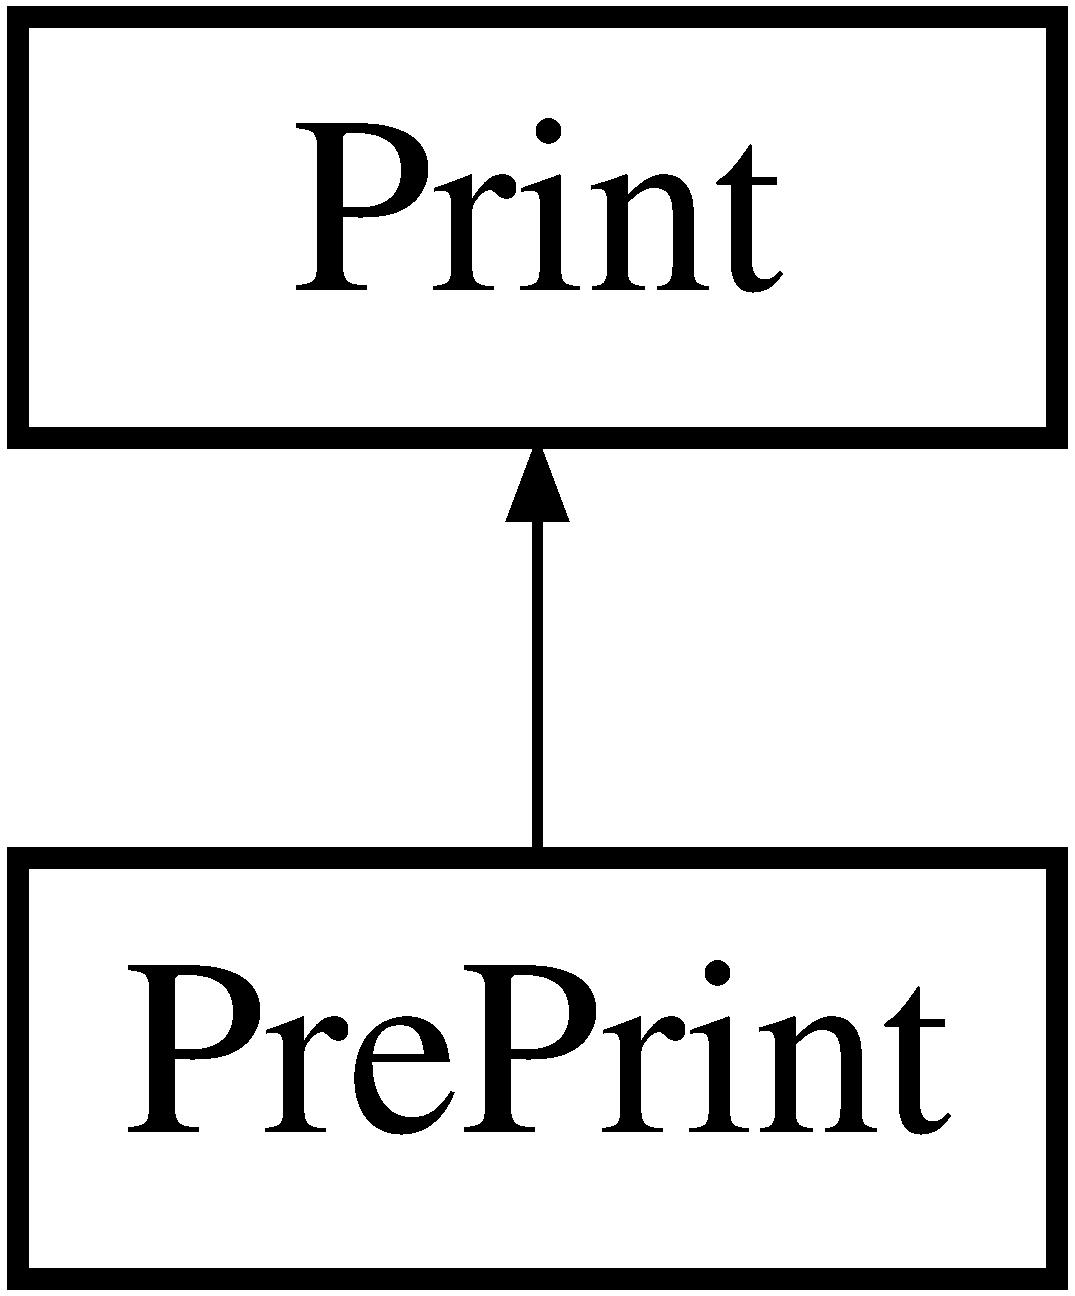
\includegraphics[height=2.000000cm]{class_pre_print}
\end{center}
\end{figure}
\subsection*{Public Member Functions}
\begin{DoxyCompactItemize}
\item 
\hyperlink{class_pre_print_a6062e08cf52ab0bacc9af9f0ea060d6d}{Pre\+Print} (Print $\ast$\hyperlink{class_pre_print_a2864325a5347e151969f30e3139d68ef}{inner\+Printer}, const char $\ast$a\+Pre\+Token, const char $\ast$a\+Post\+Token)
\item 
void \hyperlink{class_pre_print_aeb453f39e57d53c0a4fa1bdc7284209f}{set\+Inner\+Printer} (Print $\ast$\hyperlink{class_pre_print_a2864325a5347e151969f30e3139d68ef}{inner\+Printer})
\item 
virtual size\+\_\+t \hyperlink{class_pre_print_aa1a6239b213974765a39a304c18b8df3}{write} (uint8\+\_\+t c)
\end{DoxyCompactItemize}
\subsection*{Protected Member Functions}
\begin{DoxyCompactItemize}
\item 
void \hyperlink{class_pre_print_a9740712f07374dfda00d46ebf0730efc}{print\+Pre\+Token} ()
\item 
void \hyperlink{class_pre_print_a3f2ab5d0d1d614b4acf47f4ef566e428}{print\+Post\+Token} ()
\item 
void \hyperlink{class_pre_print_ac8b43aee74a660f18f3f290fc13af31e}{print\+Char} (char c)
\end{DoxyCompactItemize}
\subsection*{Protected Attributes}
\begin{DoxyCompactItemize}
\item 
\hyperlink{_pre_print_8h_a1ff8bc7546384565c03c9f1f523edab8}{Pre\+Print\+State} \hyperlink{class_pre_print_a3d55c492a2085b880305ebf9e09faa31}{state}
\item 
Print $\ast$ \hyperlink{class_pre_print_a2864325a5347e151969f30e3139d68ef}{inner\+Printer}
\item 
const char $\ast$ \hyperlink{class_pre_print_a6d490d820f913d07f7b27c3d9f7641f4}{pre\+Token}
\item 
const char $\ast$ \hyperlink{class_pre_print_a8c087522317c48cb74a26c5ac4220cc3}{post\+Token}
\end{DoxyCompactItemize}


\subsection{Detailed Description}
\hyperlink{class_pre_print}{Pre\+Print} implements Print re-\/directing all output to another print device, but with something printed before every line.
\begin{DoxyItemize}
\item Indent a printing routine.
\item prepend a comment character. 
\end{DoxyItemize}

\subsection{Constructor \& Destructor Documentation}
\hypertarget{class_pre_print_a6062e08cf52ab0bacc9af9f0ea060d6d}{}\index{Pre\+Print@{Pre\+Print}!Pre\+Print@{Pre\+Print}}
\index{Pre\+Print@{Pre\+Print}!Pre\+Print@{Pre\+Print}}
\subsubsection[{Pre\+Print(\+Print $\ast$inner\+Printer, const char $\ast$a\+Pre\+Token, const char $\ast$a\+Post\+Token)}]{\setlength{\rightskip}{0pt plus 5cm}Pre\+Print\+::\+Pre\+Print (
\begin{DoxyParamCaption}
\item[{Print $\ast$}]{inner\+Printer, }
\item[{const char $\ast$}]{a\+Pre\+Token, }
\item[{const char $\ast$}]{a\+Post\+Token}
\end{DoxyParamCaption}
)}\label{class_pre_print_a6062e08cf52ab0bacc9af9f0ea060d6d}
\hyperlink{class_capture_print}{Capture\+Print} constructor.


\begin{DoxyParams}{Parameters}
{\em inner\+Printer} & device to print to. N\+U\+L\+L to disable. \\
\hline
{\em pre\+Token} & Token to print before any line. N\+U\+L\+L to disable. \\
\hline
{\em a\+Post\+Token} & Token to print at the end of any line. N\+U\+L\+L to disable. \\
\hline
\end{DoxyParams}


\subsection{Member Function Documentation}
\hypertarget{class_pre_print_ac8b43aee74a660f18f3f290fc13af31e}{}\index{Pre\+Print@{Pre\+Print}!print\+Char@{print\+Char}}
\index{print\+Char@{print\+Char}!Pre\+Print@{Pre\+Print}}
\subsubsection[{print\+Char(char c)}]{\setlength{\rightskip}{0pt plus 5cm}void Pre\+Print\+::print\+Char (
\begin{DoxyParamCaption}
\item[{char}]{c}
\end{DoxyParamCaption}
)\hspace{0.3cm}{\ttfamily [protected]}}\label{class_pre_print_ac8b43aee74a660f18f3f290fc13af31e}
\hypertarget{class_pre_print_a3f2ab5d0d1d614b4acf47f4ef566e428}{}\index{Pre\+Print@{Pre\+Print}!print\+Post\+Token@{print\+Post\+Token}}
\index{print\+Post\+Token@{print\+Post\+Token}!Pre\+Print@{Pre\+Print}}
\subsubsection[{print\+Post\+Token()}]{\setlength{\rightskip}{0pt plus 5cm}void Pre\+Print\+::print\+Post\+Token (
\begin{DoxyParamCaption}
{}
\end{DoxyParamCaption}
)\hspace{0.3cm}{\ttfamily [protected]}}\label{class_pre_print_a3f2ab5d0d1d614b4acf47f4ef566e428}
\hypertarget{class_pre_print_a9740712f07374dfda00d46ebf0730efc}{}\index{Pre\+Print@{Pre\+Print}!print\+Pre\+Token@{print\+Pre\+Token}}
\index{print\+Pre\+Token@{print\+Pre\+Token}!Pre\+Print@{Pre\+Print}}
\subsubsection[{print\+Pre\+Token()}]{\setlength{\rightskip}{0pt plus 5cm}void Pre\+Print\+::print\+Pre\+Token (
\begin{DoxyParamCaption}
{}
\end{DoxyParamCaption}
)\hspace{0.3cm}{\ttfamily [protected]}}\label{class_pre_print_a9740712f07374dfda00d46ebf0730efc}
\hypertarget{class_pre_print_aeb453f39e57d53c0a4fa1bdc7284209f}{}\index{Pre\+Print@{Pre\+Print}!set\+Inner\+Printer@{set\+Inner\+Printer}}
\index{set\+Inner\+Printer@{set\+Inner\+Printer}!Pre\+Print@{Pre\+Print}}
\subsubsection[{set\+Inner\+Printer(\+Print $\ast$inner\+Printer)}]{\setlength{\rightskip}{0pt plus 5cm}void Pre\+Print\+::set\+Inner\+Printer (
\begin{DoxyParamCaption}
\item[{Print $\ast$}]{inner\+Printer}
\end{DoxyParamCaption}
)}\label{class_pre_print_aeb453f39e57d53c0a4fa1bdc7284209f}
Reconfigure the output device. 
\begin{DoxyParams}{Parameters}
{\em inner\+Printer} & device to print to. N\+U\+L\+L to disable. \\
\hline
\end{DoxyParams}
\hypertarget{class_pre_print_aa1a6239b213974765a39a304c18b8df3}{}\index{Pre\+Print@{Pre\+Print}!write@{write}}
\index{write@{write}!Pre\+Print@{Pre\+Print}}
\subsubsection[{write(uint8\+\_\+t c)}]{\setlength{\rightskip}{0pt plus 5cm}size\+\_\+t Pre\+Print\+::write (
\begin{DoxyParamCaption}
\item[{uint8\+\_\+t}]{c}
\end{DoxyParamCaption}
)\hspace{0.3cm}{\ttfamily [virtual]}}\label{class_pre_print_aa1a6239b213974765a39a304c18b8df3}
Write a character to the buffer. 
\begin{DoxyParams}{Parameters}
{\em c} & character to write. \\
\hline
\end{DoxyParams}


\subsection{Member Data Documentation}
\hypertarget{class_pre_print_a2864325a5347e151969f30e3139d68ef}{}\index{Pre\+Print@{Pre\+Print}!inner\+Printer@{inner\+Printer}}
\index{inner\+Printer@{inner\+Printer}!Pre\+Print@{Pre\+Print}}
\subsubsection[{inner\+Printer}]{\setlength{\rightskip}{0pt plus 5cm}Print$\ast$ Pre\+Print\+::inner\+Printer\hspace{0.3cm}{\ttfamily [protected]}}\label{class_pre_print_a2864325a5347e151969f30e3139d68ef}
\hypertarget{class_pre_print_a8c087522317c48cb74a26c5ac4220cc3}{}\index{Pre\+Print@{Pre\+Print}!post\+Token@{post\+Token}}
\index{post\+Token@{post\+Token}!Pre\+Print@{Pre\+Print}}
\subsubsection[{post\+Token}]{\setlength{\rightskip}{0pt plus 5cm}const char$\ast$ Pre\+Print\+::post\+Token\hspace{0.3cm}{\ttfamily [protected]}}\label{class_pre_print_a8c087522317c48cb74a26c5ac4220cc3}
\hypertarget{class_pre_print_a6d490d820f913d07f7b27c3d9f7641f4}{}\index{Pre\+Print@{Pre\+Print}!pre\+Token@{pre\+Token}}
\index{pre\+Token@{pre\+Token}!Pre\+Print@{Pre\+Print}}
\subsubsection[{pre\+Token}]{\setlength{\rightskip}{0pt plus 5cm}const char$\ast$ Pre\+Print\+::pre\+Token\hspace{0.3cm}{\ttfamily [protected]}}\label{class_pre_print_a6d490d820f913d07f7b27c3d9f7641f4}
\hypertarget{class_pre_print_a3d55c492a2085b880305ebf9e09faa31}{}\index{Pre\+Print@{Pre\+Print}!state@{state}}
\index{state@{state}!Pre\+Print@{Pre\+Print}}
\subsubsection[{state}]{\setlength{\rightskip}{0pt plus 5cm}{\bf Pre\+Print\+State} Pre\+Print\+::state\hspace{0.3cm}{\ttfamily [protected]}}\label{class_pre_print_a3d55c492a2085b880305ebf9e09faa31}


The documentation for this class was generated from the following files\+:\begin{DoxyCompactItemize}
\item 
W\+D\+Arduino\+Lib/src/\hyperlink{_pre_print_8h}{Pre\+Print.\+h}\item 
W\+D\+Arduino\+Lib/src/\hyperlink{_pre_print_8cpp}{Pre\+Print.\+cpp}\end{DoxyCompactItemize}

\hypertarget{class_serial_graph}{}\section{Serial\+Graph Class Reference}
\label{class_serial_graph}\index{Serial\+Graph@{Serial\+Graph}}


{\ttfamily \#include $<$Serial\+Graph.\+h$>$}

Inheritance diagram for Serial\+Graph\+:\begin{figure}[H]
\begin{center}
\leavevmode
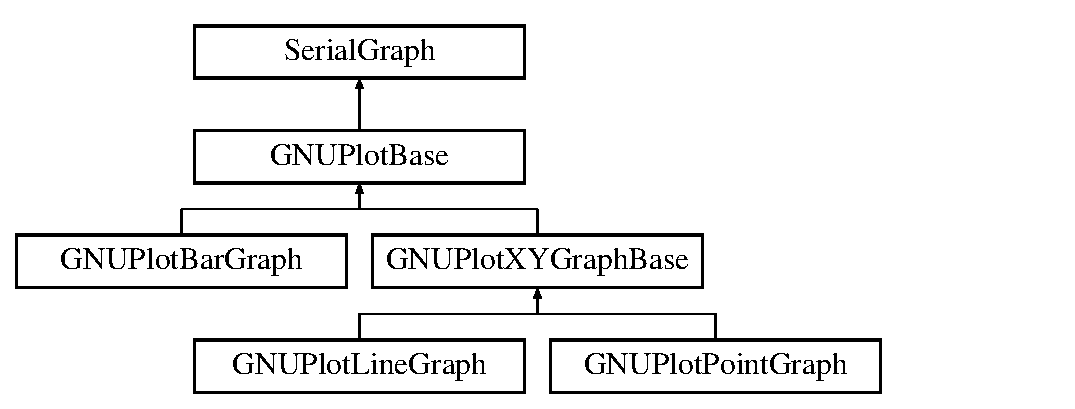
\includegraphics[height=4.000000cm]{class_serial_graph}
\end{center}
\end{figure}
\subsection*{Public Member Functions}
\begin{DoxyCompactItemize}
\item 
virtual \hyperlink{_serial_graph_8h_adc73bce6b7e6c4ecf37dde452d6a385e}{Graph\+Style} \hyperlink{class_serial_graph_a2ab97096fffdf429bfa271b9fd4c642a}{get\+Graph\+Style} () const  =0
\item 
virtual void \hyperlink{class_serial_graph_a44d34593c56aa67142ccd9fcc0a1da86}{new\+Graph} ()=0
\item 
virtual void \hyperlink{class_serial_graph_a8054ce989a1788bd35d2fde56081c88c}{finish\+Graph} ()=0
\item 
virtual void \hyperlink{class_serial_graph_a42417137c452bdc7b3ae242931ec7199}{print\+Comment\+Start} ()=0
\item 
virtual void \hyperlink{class_serial_graph_a28b020807c52c113685aa6a31f836c52}{enable\+Save\+Image\+File} (bool enabled)
\item 
virtual void \hyperlink{class_serial_graph_abf488e449d6d786bc01478793d0094ad}{set\+Show\+Grid} (bool enabled)
\item 
void \hyperlink{class_serial_graph_a4db09b008589914b71b2ee8b1873db7a}{set\+Title} (const \+\_\+\+\_\+\+Flash\+String\+Helper $\ast$title)
\item 
virtual void \hyperlink{class_serial_graph_ad726b2c84cec50c2d4bfe769e62a9bcd}{set\+Title} (const char $\ast$title)
\item 
void \hyperlink{class_serial_graph_afdb759a860c41de2fc4cfe78519b9fc0}{set\+X\+Axis\+Name} (const \+\_\+\+\_\+\+Flash\+String\+Helper $\ast$title)
\item 
virtual void \hyperlink{class_serial_graph_ac7f30036f5006091af51204a4d9efaf2}{set\+X\+Axis\+Name} (const char $\ast$name)
\item 
void \hyperlink{class_serial_graph_abfc46c15cf8e1b4362a7f51cb11c7bdb}{set\+Y\+Axis\+Name} (const \+\_\+\+\_\+\+Flash\+String\+Helper $\ast$title)
\item 
virtual void \hyperlink{class_serial_graph_ab0c675c8682959261f79dcf37b04148c}{set\+Y\+Axis\+Name} (const char $\ast$name)
\item 
virtual void \hyperlink{class_serial_graph_ae58de4fa4d391f1a2f411ce00dd74d93}{set\+X\+Axis\+Log} (byte scale)
\item 
virtual void \hyperlink{class_serial_graph_a444e38e8ef3784942ca6ee58940f7023}{set\+Y\+Axis\+Log} (byte scale)
\item 
void \hyperlink{class_serial_graph_a84d8e8ce9bff20e53ba738d1d34d3577}{set\+Series\+Name} (int \+\_\+n, const \+\_\+\+\_\+\+Flash\+String\+Helper $\ast$title)
\item 
virtual void \hyperlink{class_serial_graph_a9d67fbecbee6edb82646aa7ba5103046}{set\+Series\+Name} (int \+\_\+n, const char $\ast$name)
\item 
\hyperlink{struct_line_apperance}{Line\+Apperance} $\ast$ \hyperlink{class_serial_graph_a5a6008dc86a2101a58782929721a5b77}{get\+Line\+Apperance} (int \+\_\+n)
\item 
\hyperlink{class_serial_graph_a11529ceae46610635084b8f7d2a0dea3}{Serial\+Graph} (Print $\ast$\+\_\+out\+Stream)
\item 
virtual \hyperlink{class_serial_graph_a95d0d802bda779b43a31f29662eb9138}{$\sim$\+Serial\+Graph} ()
\item 
{\footnotesize template$<$typename Y\+T $>$ }\\void \hyperlink{class_serial_graph_afbcc26bd6bad7179d75379ac0f0d25f1}{plot\+Datum\+Y} (Y\+T y1)
\item 
{\footnotesize template$<$typename X\+T , typename Y\+T $>$ }\\void \hyperlink{class_serial_graph_a265b48fb0afe543e14cedb6619e3931e}{plot\+Datum\+X\+Y} (X\+T x, Y\+T y1)
\item 
{\footnotesize template$<$typename Y\+T $>$ }\\void \hyperlink{class_serial_graph_a56f584fa6316175bc9fbcb4f671f1c93}{plot\+Datum\+Yn} (Y\+T y1, Y\+T y2)
\item 
{\footnotesize template$<$typename Y\+T $>$ }\\void \hyperlink{class_serial_graph_ae755b026606e34c33c4aa8f10d8b5d9c}{plot\+Datum\+Yn} (Y\+T y1, Y\+T y2, Y\+T y3)
\item 
{\footnotesize template$<$typename Y\+T $>$ }\\void \hyperlink{class_serial_graph_a354feb95f91239699d3510c2ce5659b0}{plot\+Datum\+Yn} (Y\+T y1, Y\+T y2, Y\+T y3, Y\+T y4)
\item 
{\footnotesize template$<$typename Y\+T $>$ }\\void \hyperlink{class_serial_graph_ab0fff3fc1879e1cd6aadf24c913ff617}{plot\+Datum\+Yn} (Y\+T y1, Y\+T y2, Y\+T y3, Y\+T y4, Y\+T y5)
\item 
{\footnotesize template$<$typename X\+T , typename Y\+T $>$ }\\void \hyperlink{class_serial_graph_a79b721ca2be68969862869f96d6a6305}{plot\+Datum\+X\+Yn} (X\+T x, Y\+T y1, Y\+T y2)
\item 
{\footnotesize template$<$typename X\+T , typename Y\+T $>$ }\\void \hyperlink{class_serial_graph_a9fcea879f299a7d24be4ff9a38c53c26}{plot\+Datum\+X\+Yn} (X\+T x, Y\+T y1, Y\+T y2, Y\+T y3)
\item 
{\footnotesize template$<$typename X\+T , typename Y\+T $>$ }\\void \hyperlink{class_serial_graph_afd854b631604abe2014a1bb1beeeec52}{plot\+Datum\+X\+Yn} (X\+T x, Y\+T y1, Y\+T y2, Y\+T y3, Y\+T y4)
\item 
{\footnotesize template$<$typename X\+T , typename Y\+T $>$ }\\void \hyperlink{class_serial_graph_aa1bb6fa08a8bd06c074ac2a02b3f6fbc}{plot\+Datum\+X\+Yn} (X\+T x, Y\+T y1, Y\+T y2, Y\+T y3, Y\+T y4, Y\+T y5)
\item 
{\footnotesize template$<$typename X\+T , typename Y\+T $>$ }\\void \hyperlink{class_serial_graph_a3d7276c89235dc1aa176e2439ad9835b}{plot\+Datum\+X\+Yn} (X\+T x, const Y\+T $\ast$y\+Vec, int \+\_\+n)
\item 
{\footnotesize template$<$typename X\+T , typename Y\+T $>$ }\\void \hyperlink{class_serial_graph_aa20b03efac52c18c50efc79c6459a9fc}{plot\+Datum\+Yn} (const Y\+T $\ast$y\+Vec, int \+\_\+n)
\item 
{\footnotesize template$<$typename W\+T $>$ }\\void \hyperlink{class_serial_graph_aa72b48968e82a953dcdc6522bd04c7b4}{print} (const W\+T what)
\item 
{\footnotesize template$<$typename W\+T $>$ }\\void \hyperlink{class_serial_graph_a2005d103cb5a578053ef7838b3a8422d}{println} (const W\+T what)
\item 
{\footnotesize template$<$typename W\+T $>$ }\\void \hyperlink{class_serial_graph_a7237d928f67a14d5c9950d8c23c2a794}{print\+Comment} (const W\+T what)
\item 
{\footnotesize template$<$typename W\+T $>$ }\\void \hyperlink{class_serial_graph_a9b40aa22335fc26a6c29b16d278b26f8}{print\+Comment} (const W\+T $\ast$what)
\end{DoxyCompactItemize}
\subsection*{Public Attributes}
\begin{DoxyCompactItemize}
\item 
const byte \hyperlink{class_serial_graph_a1867ab3a93268646490fa7ba4f8b5680}{max\+String\+Size} = 128
\item 
const byte \hyperlink{class_serial_graph_a752a1429bd35687163fe11c5a2562bef}{max\+Series} = 8
\end{DoxyCompactItemize}
\subsection*{Protected Member Functions}
\begin{DoxyCompactItemize}
\item 
virtual void \hyperlink{class_serial_graph_a2466a642c6f6c36c708494659e975411}{print\+Seperator} ()=0
\item 
virtual void \hyperlink{class_serial_graph_ac655612a046b59c4d0f8211ed349e45c}{print\+Start\+Datum} ()=0
\item 
virtual void \hyperlink{class_serial_graph_afedf62d0e783c18e1e088d98affab108}{print\+End\+Datum} ()=0
\item 
void \hyperlink{class_serial_graph_a760dd00474c9780c81ece7cdf621fc15}{init} ()
\item 
void \hyperlink{class_serial_graph_abd43150abedec26eef3994cd33035173}{ensure\+Ready\+To\+Recive\+Plot\+Data} ()
\item 
virtual void \hyperlink{class_serial_graph_a898cf274c886e0ff45e90d3f21f0a6cc}{make\+Ready\+For\+Plot\+Data} ()
\item 
{\footnotesize template$<$typename T $>$ }\\void \hyperlink{class_serial_graph_a91e20c05c8cc612fd9ffd85880149264}{print\+Data\+Value} (T value)
\item 
virtual void \hyperlink{class_serial_graph_a8252997dd4bad0251d437d6dd097bffb}{\+\_\+print\+Data\+Value} (const char $\ast$value)
\item 
virtual void \hyperlink{class_serial_graph_a0c4d2c1239de3107d7332389183b05a1}{\+\_\+print\+Data\+Value} (const \+\_\+\+\_\+\+Flash\+String\+Helper $\ast$value)
\item 
virtual void \hyperlink{class_serial_graph_af3fbf7a9201f71cd6bad7e4337092fb6}{\+\_\+print\+Data\+Value} (char value)
\item 
virtual void \hyperlink{class_serial_graph_a58edf4683c600b6bfa1714b0f8dfc82c}{\+\_\+print\+Data\+Value} (int value)
\item 
virtual void \hyperlink{class_serial_graph_a9a4903d4fa26bb85ba5dd93c4365bcc2}{\+\_\+print\+Data\+Value} (long value)
\item 
virtual void \hyperlink{class_serial_graph_acada5333b96b65e31d8c76c3ab22905f}{\+\_\+print\+Data\+Value} (byte value)
\item 
virtual void \hyperlink{class_serial_graph_acd91cf0c3a0f49d4bdf18b447503da23}{\+\_\+print\+Data\+Value} (unsigned int value)
\item 
virtual void \hyperlink{class_serial_graph_a6dbfe61ee398e18c1b752a3748df9663}{\+\_\+print\+Data\+Value} (unsigned long value)
\item 
virtual void \hyperlink{class_serial_graph_aed9ff95634ace3d190863ea9d15c10da}{\+\_\+print\+Data\+Value} (bool value)
\item 
virtual void \hyperlink{class_serial_graph_a766d5838ede9c8fa998ce8664e5f92be}{\+\_\+print\+Data\+Value} (double value)
\end{DoxyCompactItemize}
\subsection*{Protected Attributes}
\begin{DoxyCompactItemize}
\item 
bool \hyperlink{class_serial_graph_a24202e0a7a8bac5ec1cfd92bf796e078}{save\+File}
\item 
Print $\ast$ \hyperlink{class_serial_graph_aec32289a9393e98bf80d44406e5c207d}{out\+Stream}
\item 
bool \hyperlink{class_serial_graph_a4dbd9cf190c591fb4f2f46a50d937199}{x\+Axis\+Specified}
\item 
int \hyperlink{class_serial_graph_ab40c430e06102b9624736173d4a58596}{num\+Y\+Series}
\item 
bool \hyperlink{class_serial_graph_ad61d5ea29eacc1611c5addc94714f1e2}{show\+Grid}
\item 
char $\ast$ \hyperlink{class_serial_graph_a0b33d43c2bb54340ef1f90b5f76d7aea}{graph\+Title}
\item 
char $\ast$ \hyperlink{class_serial_graph_a5f5bf85ed361ff567d0888eaa73e269c}{x\+Axis\+Name}
\item 
char $\ast$ \hyperlink{class_serial_graph_a08452a56c74ec5f5473b64605d555339}{y\+Axis\+Name}
\item 
char $\ast$$\ast$ \hyperlink{class_serial_graph_a2307e40e27249f44bbe14776dc68c561}{series\+Names}
\item 
\hyperlink{struct_line_apperance}{Line\+Apperance} $\ast$ \hyperlink{class_serial_graph_a8d743f9eeeca69a988d2159a405e4253}{series\+Apperance}
\item 
byte \hyperlink{class_serial_graph_afc2ca72fdfe2bc5e3159c9e910a8f81e}{x\+Axis\+Log\+Scale}
\item 
byte \hyperlink{class_serial_graph_a1f0424857ec14c176747b3ddb0768eee}{y\+Axis\+Log\+Scale}
\end{DoxyCompactItemize}


\subsection{Detailed Description}
A base class for creating graphs via terminal commands issues via a device inheriting from print (comm port, file, telnet).

I could see no good reason for extensive getters, as this is a \textquotesingle{}setup and and execute\textquotesingle{} type class.

\begin{DoxyNote}{Note}
Some dynamic memory usage, The caller should refrain from using malloc during plotting operations to prevent possible heap fragmentation. Dynamic memory usage is a design decision I made weighing pro\textquotesingle{}s and con\textquotesingle{}s of the situation. Given \textquotesingle{}typical usage\textquotesingle{} scenarios of the A\+P\+I it should not cause heap fragmentation.

Starting \char`\"{}another plot\char`\"{} , I strongly recomend you call \hyperlink{class_serial_graph_a44d34593c56aa67142ccd9fcc0a1da86}{new\+Graph()} first, then change the series names and other test labels. This will free all labels, preventing memory fragmentation. 
\end{DoxyNote}


\subsection{Constructor \& Destructor Documentation}
\hypertarget{class_serial_graph_a11529ceae46610635084b8f7d2a0dea3}{}\index{Serial\+Graph@{Serial\+Graph}!Serial\+Graph@{Serial\+Graph}}
\index{Serial\+Graph@{Serial\+Graph}!Serial\+Graph@{Serial\+Graph}}
\subsubsection[{Serial\+Graph(\+Print $\ast$\+\_\+out\+Stream)}]{\setlength{\rightskip}{0pt plus 5cm}Serial\+Graph\+::\+Serial\+Graph (
\begin{DoxyParamCaption}
\item[{Print $\ast$}]{\+\_\+out\+Stream}
\end{DoxyParamCaption}
)}\label{class_serial_graph_a11529ceae46610635084b8f7d2a0dea3}
Constructor. 
\begin{DoxyParams}{Parameters}
{\em \+\_\+out\+Stream} & The stream to which the (script for creating a?) graph is written. \\
\hline
\end{DoxyParams}
\hypertarget{class_serial_graph_a95d0d802bda779b43a31f29662eb9138}{}\index{Serial\+Graph@{Serial\+Graph}!````~Serial\+Graph@{$\sim$\+Serial\+Graph}}
\index{````~Serial\+Graph@{$\sim$\+Serial\+Graph}!Serial\+Graph@{Serial\+Graph}}
\subsubsection[{$\sim$\+Serial\+Graph()}]{\setlength{\rightskip}{0pt plus 5cm}Serial\+Graph\+::$\sim$\+Serial\+Graph (
\begin{DoxyParamCaption}
{}
\end{DoxyParamCaption}
)\hspace{0.3cm}{\ttfamily [virtual]}}\label{class_serial_graph_a95d0d802bda779b43a31f29662eb9138}
Destructor. I am not telling you to use it, I don\textquotesingle{}t want to debate how to employ the A\+P\+I. If you want to dispose of the graph, this will do so, releasing all dynamicaly allocated memory.

\begin{DoxyNote}{Note}
\+: If you wan\textquotesingle{}t a \char`\"{}memory breather\char`\"{} between plots, consider calling \hyperlink{class_serial_graph_a44d34593c56aa67142ccd9fcc0a1da86}{new\+Graph()}, it frees all series names, titles etc. 
\end{DoxyNote}


\subsection{Member Function Documentation}
\hypertarget{class_serial_graph_a8252997dd4bad0251d437d6dd097bffb}{}\index{Serial\+Graph@{Serial\+Graph}!\+\_\+print\+Data\+Value@{\+\_\+print\+Data\+Value}}
\index{\+\_\+print\+Data\+Value@{\+\_\+print\+Data\+Value}!Serial\+Graph@{Serial\+Graph}}
\subsubsection[{\+\_\+print\+Data\+Value(const char $\ast$value)}]{\setlength{\rightskip}{0pt plus 5cm}virtual void Serial\+Graph\+::\+\_\+print\+Data\+Value (
\begin{DoxyParamCaption}
\item[{const char $\ast$}]{value}
\end{DoxyParamCaption}
)\hspace{0.3cm}{\ttfamily [inline]}, {\ttfamily [protected]}, {\ttfamily [virtual]}}\label{class_serial_graph_a8252997dd4bad0251d437d6dd097bffb}
Override a put appropriate quotes around strings etc. 
\begin{DoxyParams}{Parameters}
{\em value} & What to print. \\
\hline
\end{DoxyParams}


Reimplemented in \hyperlink{class_g_n_u_plot_base_ad00a12fd681e4638fae005891fd72f38}{G\+N\+U\+Plot\+Base}.

\hypertarget{class_serial_graph_a0c4d2c1239de3107d7332389183b05a1}{}\index{Serial\+Graph@{Serial\+Graph}!\+\_\+print\+Data\+Value@{\+\_\+print\+Data\+Value}}
\index{\+\_\+print\+Data\+Value@{\+\_\+print\+Data\+Value}!Serial\+Graph@{Serial\+Graph}}
\subsubsection[{\+\_\+print\+Data\+Value(const \+\_\+\+\_\+\+Flash\+String\+Helper $\ast$value)}]{\setlength{\rightskip}{0pt plus 5cm}virtual void Serial\+Graph\+::\+\_\+print\+Data\+Value (
\begin{DoxyParamCaption}
\item[{const \+\_\+\+\_\+\+Flash\+String\+Helper $\ast$}]{value}
\end{DoxyParamCaption}
)\hspace{0.3cm}{\ttfamily [inline]}, {\ttfamily [protected]}, {\ttfamily [virtual]}}\label{class_serial_graph_a0c4d2c1239de3107d7332389183b05a1}
This just calls \hyperlink{class_serial_graph_a8252997dd4bad0251d437d6dd097bffb}{\+\_\+print\+Data\+Value(const char $\ast$value)} so probably alter that instead. 
\begin{DoxyParams}{Parameters}
{\em value} & What to print. \\
\hline
\end{DoxyParams}
\hypertarget{class_serial_graph_af3fbf7a9201f71cd6bad7e4337092fb6}{}\index{Serial\+Graph@{Serial\+Graph}!\+\_\+print\+Data\+Value@{\+\_\+print\+Data\+Value}}
\index{\+\_\+print\+Data\+Value@{\+\_\+print\+Data\+Value}!Serial\+Graph@{Serial\+Graph}}
\subsubsection[{\+\_\+print\+Data\+Value(char value)}]{\setlength{\rightskip}{0pt plus 5cm}virtual void Serial\+Graph\+::\+\_\+print\+Data\+Value (
\begin{DoxyParamCaption}
\item[{char}]{value}
\end{DoxyParamCaption}
)\hspace{0.3cm}{\ttfamily [inline]}, {\ttfamily [protected]}, {\ttfamily [virtual]}}\label{class_serial_graph_af3fbf7a9201f71cd6bad7e4337092fb6}
Override for customised value output. 
\begin{DoxyParams}{Parameters}
{\em value} & What to print. \\
\hline
\end{DoxyParams}


Reimplemented in \hyperlink{class_g_n_u_plot_base_aa6c6dfff0568dd99c0c28081c41b4433}{G\+N\+U\+Plot\+Base}.

\hypertarget{class_serial_graph_a58edf4683c600b6bfa1714b0f8dfc82c}{}\index{Serial\+Graph@{Serial\+Graph}!\+\_\+print\+Data\+Value@{\+\_\+print\+Data\+Value}}
\index{\+\_\+print\+Data\+Value@{\+\_\+print\+Data\+Value}!Serial\+Graph@{Serial\+Graph}}
\subsubsection[{\+\_\+print\+Data\+Value(int value)}]{\setlength{\rightskip}{0pt plus 5cm}virtual void Serial\+Graph\+::\+\_\+print\+Data\+Value (
\begin{DoxyParamCaption}
\item[{int}]{value}
\end{DoxyParamCaption}
)\hspace{0.3cm}{\ttfamily [inline]}, {\ttfamily [protected]}, {\ttfamily [virtual]}}\label{class_serial_graph_a58edf4683c600b6bfa1714b0f8dfc82c}
Override for customised value output. 
\begin{DoxyParams}{Parameters}
{\em value} & What to print. \\
\hline
\end{DoxyParams}
\hypertarget{class_serial_graph_a9a4903d4fa26bb85ba5dd93c4365bcc2}{}\index{Serial\+Graph@{Serial\+Graph}!\+\_\+print\+Data\+Value@{\+\_\+print\+Data\+Value}}
\index{\+\_\+print\+Data\+Value@{\+\_\+print\+Data\+Value}!Serial\+Graph@{Serial\+Graph}}
\subsubsection[{\+\_\+print\+Data\+Value(long value)}]{\setlength{\rightskip}{0pt plus 5cm}virtual void Serial\+Graph\+::\+\_\+print\+Data\+Value (
\begin{DoxyParamCaption}
\item[{long}]{value}
\end{DoxyParamCaption}
)\hspace{0.3cm}{\ttfamily [inline]}, {\ttfamily [protected]}, {\ttfamily [virtual]}}\label{class_serial_graph_a9a4903d4fa26bb85ba5dd93c4365bcc2}
Override for customised value output. 
\begin{DoxyParams}{Parameters}
{\em value} & What to print. \\
\hline
\end{DoxyParams}
\hypertarget{class_serial_graph_acada5333b96b65e31d8c76c3ab22905f}{}\index{Serial\+Graph@{Serial\+Graph}!\+\_\+print\+Data\+Value@{\+\_\+print\+Data\+Value}}
\index{\+\_\+print\+Data\+Value@{\+\_\+print\+Data\+Value}!Serial\+Graph@{Serial\+Graph}}
\subsubsection[{\+\_\+print\+Data\+Value(byte value)}]{\setlength{\rightskip}{0pt plus 5cm}virtual void Serial\+Graph\+::\+\_\+print\+Data\+Value (
\begin{DoxyParamCaption}
\item[{byte}]{value}
\end{DoxyParamCaption}
)\hspace{0.3cm}{\ttfamily [inline]}, {\ttfamily [protected]}, {\ttfamily [virtual]}}\label{class_serial_graph_acada5333b96b65e31d8c76c3ab22905f}
Override for customised value output. 
\begin{DoxyParams}{Parameters}
{\em value} & What to print. \\
\hline
\end{DoxyParams}
\hypertarget{class_serial_graph_acd91cf0c3a0f49d4bdf18b447503da23}{}\index{Serial\+Graph@{Serial\+Graph}!\+\_\+print\+Data\+Value@{\+\_\+print\+Data\+Value}}
\index{\+\_\+print\+Data\+Value@{\+\_\+print\+Data\+Value}!Serial\+Graph@{Serial\+Graph}}
\subsubsection[{\+\_\+print\+Data\+Value(unsigned int value)}]{\setlength{\rightskip}{0pt plus 5cm}virtual void Serial\+Graph\+::\+\_\+print\+Data\+Value (
\begin{DoxyParamCaption}
\item[{unsigned int}]{value}
\end{DoxyParamCaption}
)\hspace{0.3cm}{\ttfamily [inline]}, {\ttfamily [protected]}, {\ttfamily [virtual]}}\label{class_serial_graph_acd91cf0c3a0f49d4bdf18b447503da23}
Override for customised value output. 
\begin{DoxyParams}{Parameters}
{\em value} & What to print. \\
\hline
\end{DoxyParams}
\hypertarget{class_serial_graph_a6dbfe61ee398e18c1b752a3748df9663}{}\index{Serial\+Graph@{Serial\+Graph}!\+\_\+print\+Data\+Value@{\+\_\+print\+Data\+Value}}
\index{\+\_\+print\+Data\+Value@{\+\_\+print\+Data\+Value}!Serial\+Graph@{Serial\+Graph}}
\subsubsection[{\+\_\+print\+Data\+Value(unsigned long value)}]{\setlength{\rightskip}{0pt plus 5cm}virtual void Serial\+Graph\+::\+\_\+print\+Data\+Value (
\begin{DoxyParamCaption}
\item[{unsigned long}]{value}
\end{DoxyParamCaption}
)\hspace{0.3cm}{\ttfamily [inline]}, {\ttfamily [protected]}, {\ttfamily [virtual]}}\label{class_serial_graph_a6dbfe61ee398e18c1b752a3748df9663}
Override for customised value output. 
\begin{DoxyParams}{Parameters}
{\em value} & What to print. \\
\hline
\end{DoxyParams}
\hypertarget{class_serial_graph_aed9ff95634ace3d190863ea9d15c10da}{}\index{Serial\+Graph@{Serial\+Graph}!\+\_\+print\+Data\+Value@{\+\_\+print\+Data\+Value}}
\index{\+\_\+print\+Data\+Value@{\+\_\+print\+Data\+Value}!Serial\+Graph@{Serial\+Graph}}
\subsubsection[{\+\_\+print\+Data\+Value(bool value)}]{\setlength{\rightskip}{0pt plus 5cm}virtual void Serial\+Graph\+::\+\_\+print\+Data\+Value (
\begin{DoxyParamCaption}
\item[{bool}]{value}
\end{DoxyParamCaption}
)\hspace{0.3cm}{\ttfamily [inline]}, {\ttfamily [protected]}, {\ttfamily [virtual]}}\label{class_serial_graph_aed9ff95634ace3d190863ea9d15c10da}
Override for customised value output. 
\begin{DoxyParams}{Parameters}
{\em value} & What to print. \\
\hline
\end{DoxyParams}


Reimplemented in \hyperlink{class_g_n_u_plot_base_a6f14fc040ff833c685ab09fc7917e059}{G\+N\+U\+Plot\+Base}.

\hypertarget{class_serial_graph_a766d5838ede9c8fa998ce8664e5f92be}{}\index{Serial\+Graph@{Serial\+Graph}!\+\_\+print\+Data\+Value@{\+\_\+print\+Data\+Value}}
\index{\+\_\+print\+Data\+Value@{\+\_\+print\+Data\+Value}!Serial\+Graph@{Serial\+Graph}}
\subsubsection[{\+\_\+print\+Data\+Value(double value)}]{\setlength{\rightskip}{0pt plus 5cm}virtual void Serial\+Graph\+::\+\_\+print\+Data\+Value (
\begin{DoxyParamCaption}
\item[{double}]{value}
\end{DoxyParamCaption}
)\hspace{0.3cm}{\ttfamily [inline]}, {\ttfamily [protected]}, {\ttfamily [virtual]}}\label{class_serial_graph_a766d5838ede9c8fa998ce8664e5f92be}
Override for customised value output. 
\begin{DoxyParams}{Parameters}
{\em value} & What to print. \\
\hline
\end{DoxyParams}
\hypertarget{class_serial_graph_a28b020807c52c113685aa6a31f836c52}{}\index{Serial\+Graph@{Serial\+Graph}!enable\+Save\+Image\+File@{enable\+Save\+Image\+File}}
\index{enable\+Save\+Image\+File@{enable\+Save\+Image\+File}!Serial\+Graph@{Serial\+Graph}}
\subsubsection[{enable\+Save\+Image\+File(bool enabled)}]{\setlength{\rightskip}{0pt plus 5cm}virtual void Serial\+Graph\+::enable\+Save\+Image\+File (
\begin{DoxyParamCaption}
\item[{bool}]{enabled}
\end{DoxyParamCaption}
)\hspace{0.3cm}{\ttfamily [inline]}, {\ttfamily [virtual]}}\label{class_serial_graph_a28b020807c52c113685aa6a31f836c52}
Set to true if an image file should be saved. \begin{DoxyNote}{Note}
Filename will be based on graph title. This is done to save memory. Final filename has some extra validation performed to conform with filename rules aplicable to modern operating systems (excluding 8 char limit). 
\end{DoxyNote}
\hypertarget{class_serial_graph_abd43150abedec26eef3994cd33035173}{}\index{Serial\+Graph@{Serial\+Graph}!ensure\+Ready\+To\+Recive\+Plot\+Data@{ensure\+Ready\+To\+Recive\+Plot\+Data}}
\index{ensure\+Ready\+To\+Recive\+Plot\+Data@{ensure\+Ready\+To\+Recive\+Plot\+Data}!Serial\+Graph@{Serial\+Graph}}
\subsubsection[{ensure\+Ready\+To\+Recive\+Plot\+Data()}]{\setlength{\rightskip}{0pt plus 5cm}void Serial\+Graph\+::ensure\+Ready\+To\+Recive\+Plot\+Data (
\begin{DoxyParamCaption}
{}
\end{DoxyParamCaption}
)\hspace{0.3cm}{\ttfamily [protected]}}\label{class_serial_graph_abd43150abedec26eef3994cd33035173}
Called by every plot command prior to sending data. it\textquotesingle{}s function is to call \hyperlink{class_serial_graph_a898cf274c886e0ff45e90d3f21f0a6cc}{make\+Ready\+For\+Plot\+Data()} the first time it is called. 
\begin{DoxyParams}{Parameters}
{\em value} & What to print. \\
\hline
\end{DoxyParams}
\hypertarget{class_serial_graph_a8054ce989a1788bd35d2fde56081c88c}{}\index{Serial\+Graph@{Serial\+Graph}!finish\+Graph@{finish\+Graph}}
\index{finish\+Graph@{finish\+Graph}!Serial\+Graph@{Serial\+Graph}}
\subsubsection[{finish\+Graph()=0}]{\setlength{\rightskip}{0pt plus 5cm}virtual void Serial\+Graph\+::finish\+Graph (
\begin{DoxyParamCaption}
{}
\end{DoxyParamCaption}
)\hspace{0.3cm}{\ttfamily [pure virtual]}}\label{class_serial_graph_a8054ce989a1788bd35d2fde56081c88c}
Serial output that finishes the plot, saves file, updates display etc. 

Implemented in \hyperlink{class_g_n_u_plot_base_aa4b0574c35fbee4dc5f25451eaf956dd}{G\+N\+U\+Plot\+Base}.

\hypertarget{class_serial_graph_a2ab97096fffdf429bfa271b9fd4c642a}{}\index{Serial\+Graph@{Serial\+Graph}!get\+Graph\+Style@{get\+Graph\+Style}}
\index{get\+Graph\+Style@{get\+Graph\+Style}!Serial\+Graph@{Serial\+Graph}}
\subsubsection[{get\+Graph\+Style() const  =0}]{\setlength{\rightskip}{0pt plus 5cm}virtual {\bf Graph\+Style} Serial\+Graph\+::get\+Graph\+Style (
\begin{DoxyParamCaption}
{}
\end{DoxyParamCaption}
) const\hspace{0.3cm}{\ttfamily [pure virtual]}}\label{class_serial_graph_a2ab97096fffdf429bfa271b9fd4c642a}
Returns the Graph\+Style of the current object. 

Implemented in \hyperlink{class_g_n_u_plot_bar_graph_a6b2cde2832fcb246361d8ebddbe7a228}{G\+N\+U\+Plot\+Bar\+Graph}, \hyperlink{class_g_n_u_plot_point_graph_aeeae395426112202d3617ff66d836c99}{G\+N\+U\+Plot\+Point\+Graph}, and \hyperlink{class_g_n_u_plot_line_graph_a8f8b19efd8d8f4f25ccc41635e332593}{G\+N\+U\+Plot\+Line\+Graph}.

\hypertarget{class_serial_graph_a5a6008dc86a2101a58782929721a5b77}{}\index{Serial\+Graph@{Serial\+Graph}!get\+Line\+Apperance@{get\+Line\+Apperance}}
\index{get\+Line\+Apperance@{get\+Line\+Apperance}!Serial\+Graph@{Serial\+Graph}}
\subsubsection[{get\+Line\+Apperance(int \+\_\+n)}]{\setlength{\rightskip}{0pt plus 5cm}{\bf Line\+Apperance}$\ast$ Serial\+Graph\+::get\+Line\+Apperance (
\begin{DoxyParamCaption}
\item[{int}]{\+\_\+n}
\end{DoxyParamCaption}
)\hspace{0.3cm}{\ttfamily [inline]}}\label{class_serial_graph_a5a6008dc86a2101a58782929721a5b77}
Gets a structure that controls apperance of a series (called a \hyperlink{struct_line_apperance}{Line\+Apperance}). It is intended that you directly modify the structure returned, there is no set\+Line\+Apperance. See the struct \hyperlink{struct_line_apperance}{Line\+Apperance} for more.


\begin{DoxyParams}{Parameters}
{\em \+\_\+n} & Series number to alter.\\
\hline
\end{DoxyParams}
\begin{DoxyNote}{Note}
Behaviour on \+\_\+n $>$ max\+Series, is to just override the last possible series entry. 
\end{DoxyNote}
\hypertarget{class_serial_graph_a760dd00474c9780c81ece7cdf621fc15}{}\index{Serial\+Graph@{Serial\+Graph}!init@{init}}
\index{init@{init}!Serial\+Graph@{Serial\+Graph}}
\subsubsection[{init()}]{\setlength{\rightskip}{0pt plus 5cm}void Serial\+Graph\+::init (
\begin{DoxyParamCaption}
{}
\end{DoxyParamCaption}
)\hspace{0.3cm}{\ttfamily [protected]}}\label{class_serial_graph_a760dd00474c9780c81ece7cdf621fc15}
Brings the class to its default state. Called by the constructor and \hyperlink{class_serial_graph_a44d34593c56aa67142ccd9fcc0a1da86}{new\+Graph()}. \hypertarget{class_serial_graph_a898cf274c886e0ff45e90d3f21f0a6cc}{}\index{Serial\+Graph@{Serial\+Graph}!make\+Ready\+For\+Plot\+Data@{make\+Ready\+For\+Plot\+Data}}
\index{make\+Ready\+For\+Plot\+Data@{make\+Ready\+For\+Plot\+Data}!Serial\+Graph@{Serial\+Graph}}
\subsubsection[{make\+Ready\+For\+Plot\+Data()}]{\setlength{\rightskip}{0pt plus 5cm}void Serial\+Graph\+::make\+Ready\+For\+Plot\+Data (
\begin{DoxyParamCaption}
{}
\end{DoxyParamCaption}
)\hspace{0.3cm}{\ttfamily [protected]}, {\ttfamily [virtual]}}\label{class_serial_graph_a898cf274c886e0ff45e90d3f21f0a6cc}
Called by ensure\+Ready\+To\+Recive\+Plot\+Data, if the first plot command is encountered. \begin{DoxyNote}{Note}
A concrete class should override this. 
\end{DoxyNote}


Reimplemented in \hyperlink{class_g_n_u_plot_base_adaf91c191e4d889537d401faeb863485}{G\+N\+U\+Plot\+Base}.

\hypertarget{class_serial_graph_a44d34593c56aa67142ccd9fcc0a1da86}{}\index{Serial\+Graph@{Serial\+Graph}!new\+Graph@{new\+Graph}}
\index{new\+Graph@{new\+Graph}!Serial\+Graph@{Serial\+Graph}}
\subsubsection[{new\+Graph()=0}]{\setlength{\rightskip}{0pt plus 5cm}virtual void Serial\+Graph\+::new\+Graph (
\begin{DoxyParamCaption}
{}
\end{DoxyParamCaption}
)\hspace{0.3cm}{\ttfamily [pure virtual]}}\label{class_serial_graph_a44d34593c56aa67142ccd9fcc0a1da86}
Serial output that establishes a new graph. This should also call \hyperlink{class_serial_graph_a760dd00474c9780c81ece7cdf621fc15}{init()}, to reset the class. \begin{DoxyNote}{Note}
\+: If you wan\textquotesingle{}t a \char`\"{}memory breather\char`\"{} between plots, calling this method frees all series names, titles etc. 
\end{DoxyNote}


Implemented in \hyperlink{class_g_n_u_plot_base_a4d4da234cfdeb99ec3228ef7b2df8a50}{G\+N\+U\+Plot\+Base}.

\hypertarget{class_serial_graph_a265b48fb0afe543e14cedb6619e3931e}{}\index{Serial\+Graph@{Serial\+Graph}!plot\+Datum\+X\+Y@{plot\+Datum\+X\+Y}}
\index{plot\+Datum\+X\+Y@{plot\+Datum\+X\+Y}!Serial\+Graph@{Serial\+Graph}}
\subsubsection[{plot\+Datum\+X\+Y(\+X\+T x, Y\+T y1)}]{\setlength{\rightskip}{0pt plus 5cm}template$<$typename X\+T , typename Y\+T $>$ void Serial\+Graph\+::plot\+Datum\+X\+Y (
\begin{DoxyParamCaption}
\item[{X\+T}]{x, }
\item[{Y\+T}]{y1}
\end{DoxyParamCaption}
)\hspace{0.3cm}{\ttfamily [inline]}}\label{class_serial_graph_a265b48fb0afe543e14cedb6619e3931e}
Outputs a point to be plotted. All Y values must be of the same type.

\begin{DoxyNote}{Note}
The first time this is called after \hyperlink{class_serial_graph_a44d34593c56aa67142ccd9fcc0a1da86}{new\+Graph()}, \hyperlink{class_serial_graph_a898cf274c886e0ff45e90d3f21f0a6cc}{make\+Ready\+For\+Plot\+Data()} will be called. 

The following feilds automatically set\+: x\+Axis\+Specified; num\+Y\+Series; 
\end{DoxyNote}
\hypertarget{class_serial_graph_a79b721ca2be68969862869f96d6a6305}{}\index{Serial\+Graph@{Serial\+Graph}!plot\+Datum\+X\+Yn@{plot\+Datum\+X\+Yn}}
\index{plot\+Datum\+X\+Yn@{plot\+Datum\+X\+Yn}!Serial\+Graph@{Serial\+Graph}}
\subsubsection[{plot\+Datum\+X\+Yn(\+X\+T x, Y\+T y1, Y\+T y2)}]{\setlength{\rightskip}{0pt plus 5cm}template$<$typename X\+T , typename Y\+T $>$ void Serial\+Graph\+::plot\+Datum\+X\+Yn (
\begin{DoxyParamCaption}
\item[{X\+T}]{x, }
\item[{Y\+T}]{y1, }
\item[{Y\+T}]{y2}
\end{DoxyParamCaption}
)\hspace{0.3cm}{\ttfamily [inline]}}\label{class_serial_graph_a79b721ca2be68969862869f96d6a6305}
Outputs a point to be plotted. All Y values must be of the same type.

\begin{DoxyNote}{Note}
The first time this is called after \hyperlink{class_serial_graph_a44d34593c56aa67142ccd9fcc0a1da86}{new\+Graph()}, \hyperlink{class_serial_graph_a898cf274c886e0ff45e90d3f21f0a6cc}{make\+Ready\+For\+Plot\+Data()} will be called. 

The following feilds automatically set\+: x\+Axis\+Specified; num\+Y\+Series; 
\end{DoxyNote}
\hypertarget{class_serial_graph_a9fcea879f299a7d24be4ff9a38c53c26}{}\index{Serial\+Graph@{Serial\+Graph}!plot\+Datum\+X\+Yn@{plot\+Datum\+X\+Yn}}
\index{plot\+Datum\+X\+Yn@{plot\+Datum\+X\+Yn}!Serial\+Graph@{Serial\+Graph}}
\subsubsection[{plot\+Datum\+X\+Yn(\+X\+T x, Y\+T y1, Y\+T y2, Y\+T y3)}]{\setlength{\rightskip}{0pt plus 5cm}template$<$typename X\+T , typename Y\+T $>$ void Serial\+Graph\+::plot\+Datum\+X\+Yn (
\begin{DoxyParamCaption}
\item[{X\+T}]{x, }
\item[{Y\+T}]{y1, }
\item[{Y\+T}]{y2, }
\item[{Y\+T}]{y3}
\end{DoxyParamCaption}
)\hspace{0.3cm}{\ttfamily [inline]}}\label{class_serial_graph_a9fcea879f299a7d24be4ff9a38c53c26}
Outputs a point to be plotted. All Y values must be of the same type.

\begin{DoxyNote}{Note}
The first time this is called after \hyperlink{class_serial_graph_a44d34593c56aa67142ccd9fcc0a1da86}{new\+Graph()}, \hyperlink{class_serial_graph_a898cf274c886e0ff45e90d3f21f0a6cc}{make\+Ready\+For\+Plot\+Data()} will be called. 

The following feilds automatically set\+: x\+Axis\+Specified; num\+Y\+Series; 
\end{DoxyNote}
\hypertarget{class_serial_graph_afd854b631604abe2014a1bb1beeeec52}{}\index{Serial\+Graph@{Serial\+Graph}!plot\+Datum\+X\+Yn@{plot\+Datum\+X\+Yn}}
\index{plot\+Datum\+X\+Yn@{plot\+Datum\+X\+Yn}!Serial\+Graph@{Serial\+Graph}}
\subsubsection[{plot\+Datum\+X\+Yn(\+X\+T x, Y\+T y1, Y\+T y2, Y\+T y3, Y\+T y4)}]{\setlength{\rightskip}{0pt plus 5cm}template$<$typename X\+T , typename Y\+T $>$ void Serial\+Graph\+::plot\+Datum\+X\+Yn (
\begin{DoxyParamCaption}
\item[{X\+T}]{x, }
\item[{Y\+T}]{y1, }
\item[{Y\+T}]{y2, }
\item[{Y\+T}]{y3, }
\item[{Y\+T}]{y4}
\end{DoxyParamCaption}
)\hspace{0.3cm}{\ttfamily [inline]}}\label{class_serial_graph_afd854b631604abe2014a1bb1beeeec52}
Outputs a point to be plotted. All Y values must be of the same type.

\begin{DoxyNote}{Note}
The first time this is called after \hyperlink{class_serial_graph_a44d34593c56aa67142ccd9fcc0a1da86}{new\+Graph()}, \hyperlink{class_serial_graph_a898cf274c886e0ff45e90d3f21f0a6cc}{make\+Ready\+For\+Plot\+Data()} will be called. 

The following feilds automatically set\+: x\+Axis\+Specified; num\+Y\+Series; 
\end{DoxyNote}
\hypertarget{class_serial_graph_aa1bb6fa08a8bd06c074ac2a02b3f6fbc}{}\index{Serial\+Graph@{Serial\+Graph}!plot\+Datum\+X\+Yn@{plot\+Datum\+X\+Yn}}
\index{plot\+Datum\+X\+Yn@{plot\+Datum\+X\+Yn}!Serial\+Graph@{Serial\+Graph}}
\subsubsection[{plot\+Datum\+X\+Yn(\+X\+T x, Y\+T y1, Y\+T y2, Y\+T y3, Y\+T y4, Y\+T y5)}]{\setlength{\rightskip}{0pt plus 5cm}template$<$typename X\+T , typename Y\+T $>$ void Serial\+Graph\+::plot\+Datum\+X\+Yn (
\begin{DoxyParamCaption}
\item[{X\+T}]{x, }
\item[{Y\+T}]{y1, }
\item[{Y\+T}]{y2, }
\item[{Y\+T}]{y3, }
\item[{Y\+T}]{y4, }
\item[{Y\+T}]{y5}
\end{DoxyParamCaption}
)\hspace{0.3cm}{\ttfamily [inline]}}\label{class_serial_graph_aa1bb6fa08a8bd06c074ac2a02b3f6fbc}
Outputs a point to be plotted. All Y values must be of the same type.

\begin{DoxyNote}{Note}
The first time this is called after \hyperlink{class_serial_graph_a44d34593c56aa67142ccd9fcc0a1da86}{new\+Graph()}, \hyperlink{class_serial_graph_a898cf274c886e0ff45e90d3f21f0a6cc}{make\+Ready\+For\+Plot\+Data()} will be called. 

The following feilds automatically set\+: x\+Axis\+Specified; num\+Y\+Series; 
\end{DoxyNote}
\hypertarget{class_serial_graph_a3d7276c89235dc1aa176e2439ad9835b}{}\index{Serial\+Graph@{Serial\+Graph}!plot\+Datum\+X\+Yn@{plot\+Datum\+X\+Yn}}
\index{plot\+Datum\+X\+Yn@{plot\+Datum\+X\+Yn}!Serial\+Graph@{Serial\+Graph}}
\subsubsection[{plot\+Datum\+X\+Yn(\+X\+T x, const Y\+T $\ast$y\+Vec, int \+\_\+n)}]{\setlength{\rightskip}{0pt plus 5cm}template$<$typename X\+T , typename Y\+T $>$ void Serial\+Graph\+::plot\+Datum\+X\+Yn (
\begin{DoxyParamCaption}
\item[{X\+T}]{x, }
\item[{const Y\+T $\ast$}]{y\+Vec, }
\item[{int}]{\+\_\+n}
\end{DoxyParamCaption}
)\hspace{0.3cm}{\ttfamily [inline]}}\label{class_serial_graph_a3d7276c89235dc1aa176e2439ad9835b}
Outputs a point to be plotted. All Y values must be of the same type.


\begin{DoxyParams}{Parameters}
{\em y\+Vec} & Pointer to an array of y\+Values. \\
\hline
{\em \+\_\+n} & Number of items in array.\\
\hline
\end{DoxyParams}
\begin{DoxyNote}{Note}
Behaviour on \+\_\+n $>$ max\+Series, is to just override the last possible series entry. 
\end{DoxyNote}
\hypertarget{class_serial_graph_afbcc26bd6bad7179d75379ac0f0d25f1}{}\index{Serial\+Graph@{Serial\+Graph}!plot\+Datum\+Y@{plot\+Datum\+Y}}
\index{plot\+Datum\+Y@{plot\+Datum\+Y}!Serial\+Graph@{Serial\+Graph}}
\subsubsection[{plot\+Datum\+Y(\+Y\+T y1)}]{\setlength{\rightskip}{0pt plus 5cm}template$<$typename Y\+T $>$ void Serial\+Graph\+::plot\+Datum\+Y (
\begin{DoxyParamCaption}
\item[{Y\+T}]{y1}
\end{DoxyParamCaption}
)\hspace{0.3cm}{\ttfamily [inline]}}\label{class_serial_graph_afbcc26bd6bad7179d75379ac0f0d25f1}
Outputs a point to be plotted. All Y values must be of the same type.

\begin{DoxyNote}{Note}
The first time this is called after \hyperlink{class_serial_graph_a44d34593c56aa67142ccd9fcc0a1da86}{new\+Graph()}, \hyperlink{class_serial_graph_a898cf274c886e0ff45e90d3f21f0a6cc}{make\+Ready\+For\+Plot\+Data()} will be called. 

The following feilds automatically set\+: x\+Axis\+Specified; num\+Y\+Series; 
\end{DoxyNote}
\hypertarget{class_serial_graph_a56f584fa6316175bc9fbcb4f671f1c93}{}\index{Serial\+Graph@{Serial\+Graph}!plot\+Datum\+Yn@{plot\+Datum\+Yn}}
\index{plot\+Datum\+Yn@{plot\+Datum\+Yn}!Serial\+Graph@{Serial\+Graph}}
\subsubsection[{plot\+Datum\+Yn(\+Y\+T y1, Y\+T y2)}]{\setlength{\rightskip}{0pt plus 5cm}template$<$typename Y\+T $>$ void Serial\+Graph\+::plot\+Datum\+Yn (
\begin{DoxyParamCaption}
\item[{Y\+T}]{y1, }
\item[{Y\+T}]{y2}
\end{DoxyParamCaption}
)\hspace{0.3cm}{\ttfamily [inline]}}\label{class_serial_graph_a56f584fa6316175bc9fbcb4f671f1c93}
Outputs a point to be plotted. All Y values must be of the same type.

\begin{DoxyNote}{Note}
The first time this is called after \hyperlink{class_serial_graph_a44d34593c56aa67142ccd9fcc0a1da86}{new\+Graph()}, \hyperlink{class_serial_graph_a898cf274c886e0ff45e90d3f21f0a6cc}{make\+Ready\+For\+Plot\+Data()} will be called. 

The following feilds automatically set\+: x\+Axis\+Specified; num\+Y\+Series; 
\end{DoxyNote}
\hypertarget{class_serial_graph_ae755b026606e34c33c4aa8f10d8b5d9c}{}\index{Serial\+Graph@{Serial\+Graph}!plot\+Datum\+Yn@{plot\+Datum\+Yn}}
\index{plot\+Datum\+Yn@{plot\+Datum\+Yn}!Serial\+Graph@{Serial\+Graph}}
\subsubsection[{plot\+Datum\+Yn(\+Y\+T y1, Y\+T y2, Y\+T y3)}]{\setlength{\rightskip}{0pt plus 5cm}template$<$typename Y\+T $>$ void Serial\+Graph\+::plot\+Datum\+Yn (
\begin{DoxyParamCaption}
\item[{Y\+T}]{y1, }
\item[{Y\+T}]{y2, }
\item[{Y\+T}]{y3}
\end{DoxyParamCaption}
)\hspace{0.3cm}{\ttfamily [inline]}}\label{class_serial_graph_ae755b026606e34c33c4aa8f10d8b5d9c}
Outputs a point to be plotted. All Y values must be of the same type.

\begin{DoxyNote}{Note}
The first time this is called after \hyperlink{class_serial_graph_a44d34593c56aa67142ccd9fcc0a1da86}{new\+Graph()}, \hyperlink{class_serial_graph_a898cf274c886e0ff45e90d3f21f0a6cc}{make\+Ready\+For\+Plot\+Data()} will be called. 

The following feilds automatically set\+: x\+Axis\+Specified; num\+Y\+Series; 
\end{DoxyNote}
\hypertarget{class_serial_graph_a354feb95f91239699d3510c2ce5659b0}{}\index{Serial\+Graph@{Serial\+Graph}!plot\+Datum\+Yn@{plot\+Datum\+Yn}}
\index{plot\+Datum\+Yn@{plot\+Datum\+Yn}!Serial\+Graph@{Serial\+Graph}}
\subsubsection[{plot\+Datum\+Yn(\+Y\+T y1, Y\+T y2, Y\+T y3, Y\+T y4)}]{\setlength{\rightskip}{0pt plus 5cm}template$<$typename Y\+T $>$ void Serial\+Graph\+::plot\+Datum\+Yn (
\begin{DoxyParamCaption}
\item[{Y\+T}]{y1, }
\item[{Y\+T}]{y2, }
\item[{Y\+T}]{y3, }
\item[{Y\+T}]{y4}
\end{DoxyParamCaption}
)\hspace{0.3cm}{\ttfamily [inline]}}\label{class_serial_graph_a354feb95f91239699d3510c2ce5659b0}
Outputs a point to be plotted. All Y values must be of the same type.

\begin{DoxyNote}{Note}
The first time this is called after \hyperlink{class_serial_graph_a44d34593c56aa67142ccd9fcc0a1da86}{new\+Graph()}, \hyperlink{class_serial_graph_a898cf274c886e0ff45e90d3f21f0a6cc}{make\+Ready\+For\+Plot\+Data()} will be called. 

The following feilds automatically set\+: x\+Axis\+Specified; num\+Y\+Series; 
\end{DoxyNote}
\hypertarget{class_serial_graph_ab0fff3fc1879e1cd6aadf24c913ff617}{}\index{Serial\+Graph@{Serial\+Graph}!plot\+Datum\+Yn@{plot\+Datum\+Yn}}
\index{plot\+Datum\+Yn@{plot\+Datum\+Yn}!Serial\+Graph@{Serial\+Graph}}
\subsubsection[{plot\+Datum\+Yn(\+Y\+T y1, Y\+T y2, Y\+T y3, Y\+T y4, Y\+T y5)}]{\setlength{\rightskip}{0pt plus 5cm}template$<$typename Y\+T $>$ void Serial\+Graph\+::plot\+Datum\+Yn (
\begin{DoxyParamCaption}
\item[{Y\+T}]{y1, }
\item[{Y\+T}]{y2, }
\item[{Y\+T}]{y3, }
\item[{Y\+T}]{y4, }
\item[{Y\+T}]{y5}
\end{DoxyParamCaption}
)\hspace{0.3cm}{\ttfamily [inline]}}\label{class_serial_graph_ab0fff3fc1879e1cd6aadf24c913ff617}
Outputs a point to be plotted. All Y values must be of the same type.

\begin{DoxyNote}{Note}
The first time this is called after \hyperlink{class_serial_graph_a44d34593c56aa67142ccd9fcc0a1da86}{new\+Graph()}, \hyperlink{class_serial_graph_a898cf274c886e0ff45e90d3f21f0a6cc}{make\+Ready\+For\+Plot\+Data()} will be called. 

The following feilds automatically set\+: x\+Axis\+Specified; num\+Y\+Series; 
\end{DoxyNote}
\hypertarget{class_serial_graph_aa20b03efac52c18c50efc79c6459a9fc}{}\index{Serial\+Graph@{Serial\+Graph}!plot\+Datum\+Yn@{plot\+Datum\+Yn}}
\index{plot\+Datum\+Yn@{plot\+Datum\+Yn}!Serial\+Graph@{Serial\+Graph}}
\subsubsection[{plot\+Datum\+Yn(const Y\+T $\ast$y\+Vec, int \+\_\+n)}]{\setlength{\rightskip}{0pt plus 5cm}template$<$typename X\+T , typename Y\+T $>$ void Serial\+Graph\+::plot\+Datum\+Yn (
\begin{DoxyParamCaption}
\item[{const Y\+T $\ast$}]{y\+Vec, }
\item[{int}]{\+\_\+n}
\end{DoxyParamCaption}
)\hspace{0.3cm}{\ttfamily [inline]}}\label{class_serial_graph_aa20b03efac52c18c50efc79c6459a9fc}
Outputs a point to be plotted. All Y values must be of the same type.


\begin{DoxyParams}{Parameters}
{\em y\+Vec} & Pointer to an array of y\+Values. \\
\hline
{\em \+\_\+n} & Number of items in array.\\
\hline
\end{DoxyParams}
\begin{DoxyNote}{Note}
Behaviour on \+\_\+n $>$ max\+Series, is to just override the last possible series entry. 
\end{DoxyNote}
\hypertarget{class_serial_graph_aa72b48968e82a953dcdc6522bd04c7b4}{}\index{Serial\+Graph@{Serial\+Graph}!print@{print}}
\index{print@{print}!Serial\+Graph@{Serial\+Graph}}
\subsubsection[{print(const W\+T what)}]{\setlength{\rightskip}{0pt plus 5cm}template$<$typename W\+T $>$ void Serial\+Graph\+::print (
\begin{DoxyParamCaption}
\item[{const W\+T}]{what}
\end{DoxyParamCaption}
)\hspace{0.3cm}{\ttfamily [inline]}}\label{class_serial_graph_aa72b48968e82a953dcdc6522bd04c7b4}
Outputs text directly to the graph output. To use this for debug notes etc, call \hyperlink{class_serial_graph_a42417137c452bdc7b3ae242931ec7199}{print\+Comment\+Start()} first.


\begin{DoxyParams}{Parameters}
{\em what} & Anything you can sent to a Print class. \\
\hline
\end{DoxyParams}
\begin{DoxyNote}{Note}
No string validation; as this is not considered a method that should recive data from outside the codebase. 
\end{DoxyNote}
\hypertarget{class_serial_graph_a7237d928f67a14d5c9950d8c23c2a794}{}\index{Serial\+Graph@{Serial\+Graph}!print\+Comment@{print\+Comment}}
\index{print\+Comment@{print\+Comment}!Serial\+Graph@{Serial\+Graph}}
\subsubsection[{print\+Comment(const W\+T what)}]{\setlength{\rightskip}{0pt plus 5cm}template$<$typename W\+T $>$ void Serial\+Graph\+::print\+Comment (
\begin{DoxyParamCaption}
\item[{const W\+T}]{what}
\end{DoxyParamCaption}
)\hspace{0.3cm}{\ttfamily [inline]}}\label{class_serial_graph_a7237d928f67a14d5c9950d8c23c2a794}
Outputs a comment that is ignored by the graph output. Use this for debug notes etc.


\begin{DoxyParams}{Parameters}
{\em what} & Anything you can sent to a Print class. \\
\hline
\end{DoxyParams}
\begin{DoxyNote}{Note}
No string validation; as this is not considered a method that should recive data from outside the codebase. 
\end{DoxyNote}
\hypertarget{class_serial_graph_a9b40aa22335fc26a6c29b16d278b26f8}{}\index{Serial\+Graph@{Serial\+Graph}!print\+Comment@{print\+Comment}}
\index{print\+Comment@{print\+Comment}!Serial\+Graph@{Serial\+Graph}}
\subsubsection[{print\+Comment(const W\+T $\ast$what)}]{\setlength{\rightskip}{0pt plus 5cm}template$<$typename W\+T $>$ void Serial\+Graph\+::print\+Comment (
\begin{DoxyParamCaption}
\item[{const W\+T $\ast$}]{what}
\end{DoxyParamCaption}
)\hspace{0.3cm}{\ttfamily [inline]}}\label{class_serial_graph_a9b40aa22335fc26a6c29b16d278b26f8}
Outputs a comment that is ignored by the graph output. Use this for debug notes etc.


\begin{DoxyParams}{Parameters}
{\em what} & Anything you can sent to a Print class. \\
\hline
\end{DoxyParams}
\begin{DoxyNote}{Note}
No string validation; as this is not considered a method that should recive data from outside the codebase. 
\end{DoxyNote}
\hypertarget{class_serial_graph_a42417137c452bdc7b3ae242931ec7199}{}\index{Serial\+Graph@{Serial\+Graph}!print\+Comment\+Start@{print\+Comment\+Start}}
\index{print\+Comment\+Start@{print\+Comment\+Start}!Serial\+Graph@{Serial\+Graph}}
\subsubsection[{print\+Comment\+Start()=0}]{\setlength{\rightskip}{0pt plus 5cm}virtual void Serial\+Graph\+::print\+Comment\+Start (
\begin{DoxyParamCaption}
{}
\end{DoxyParamCaption}
)\hspace{0.3cm}{\ttfamily [pure virtual]}}\label{class_serial_graph_a42417137c452bdc7b3ae242931ec7199}
Prints the text which makes a line a comment 

Implemented in \hyperlink{class_g_n_u_plot_base_a219601bd41203477ae73a18d18dd7443}{G\+N\+U\+Plot\+Base}.

\hypertarget{class_serial_graph_a91e20c05c8cc612fd9ffd85880149264}{}\index{Serial\+Graph@{Serial\+Graph}!print\+Data\+Value@{print\+Data\+Value}}
\index{print\+Data\+Value@{print\+Data\+Value}!Serial\+Graph@{Serial\+Graph}}
\subsubsection[{print\+Data\+Value(\+T value)}]{\setlength{\rightskip}{0pt plus 5cm}template$<$typename T $>$ void Serial\+Graph\+::print\+Data\+Value (
\begin{DoxyParamCaption}
\item[{T}]{value}
\end{DoxyParamCaption}
)\hspace{0.3cm}{\ttfamily [inline]}, {\ttfamily [protected]}}\label{class_serial_graph_a91e20c05c8cc612fd9ffd85880149264}
Prints plot data in a format that the server can understand. Override a coresponding \+\_\+print\+Data\+Value(...) to put appropriate quotes around strings etc.


\begin{DoxyParams}{Parameters}
{\em value} & What to print. \\
\hline
\end{DoxyParams}
\hypertarget{class_serial_graph_afedf62d0e783c18e1e088d98affab108}{}\index{Serial\+Graph@{Serial\+Graph}!print\+End\+Datum@{print\+End\+Datum}}
\index{print\+End\+Datum@{print\+End\+Datum}!Serial\+Graph@{Serial\+Graph}}
\subsubsection[{print\+End\+Datum()=0}]{\setlength{\rightskip}{0pt plus 5cm}virtual void Serial\+Graph\+::print\+End\+Datum (
\begin{DoxyParamCaption}
{}
\end{DoxyParamCaption}
)\hspace{0.3cm}{\ttfamily [protected]}, {\ttfamily [pure virtual]}}\label{class_serial_graph_afedf62d0e783c18e1e088d98affab108}
If I am plotting point x, y; then this is printed afterward. It should include out\+Stream-\/$>$\hyperlink{class_serial_graph_a2005d103cb5a578053ef7838b3a8422d}{println()}; if data is to be sent via seperate lines. 

Implemented in \hyperlink{class_g_n_u_plot_base_aff02bc279e6c3cb83f2cdc7aa021268f}{G\+N\+U\+Plot\+Base}.

\hypertarget{class_serial_graph_a2005d103cb5a578053ef7838b3a8422d}{}\index{Serial\+Graph@{Serial\+Graph}!println@{println}}
\index{println@{println}!Serial\+Graph@{Serial\+Graph}}
\subsubsection[{println(const W\+T what)}]{\setlength{\rightskip}{0pt plus 5cm}template$<$typename W\+T $>$ void Serial\+Graph\+::println (
\begin{DoxyParamCaption}
\item[{const W\+T}]{what}
\end{DoxyParamCaption}
)\hspace{0.3cm}{\ttfamily [inline]}}\label{class_serial_graph_a2005d103cb5a578053ef7838b3a8422d}
Outputs text directly to the graph output. To use this for debug notes etc, call \hyperlink{class_serial_graph_a42417137c452bdc7b3ae242931ec7199}{print\+Comment\+Start()} first.


\begin{DoxyParams}{Parameters}
{\em what} & Anything you can sent to a Print class. \\
\hline
\end{DoxyParams}
\begin{DoxyNote}{Note}
No string validation; as this is not considered a method that should recive data from outside the codebase. 
\end{DoxyNote}
\hypertarget{class_serial_graph_a2466a642c6f6c36c708494659e975411}{}\index{Serial\+Graph@{Serial\+Graph}!print\+Seperator@{print\+Seperator}}
\index{print\+Seperator@{print\+Seperator}!Serial\+Graph@{Serial\+Graph}}
\subsubsection[{print\+Seperator()=0}]{\setlength{\rightskip}{0pt plus 5cm}virtual void Serial\+Graph\+::print\+Seperator (
\begin{DoxyParamCaption}
{}
\end{DoxyParamCaption}
)\hspace{0.3cm}{\ttfamily [protected]}, {\ttfamily [pure virtual]}}\label{class_serial_graph_a2466a642c6f6c36c708494659e975411}
If I am plotting x, y1, y2; then this is the deliminator (the comma in this case) 

Implemented in \hyperlink{class_g_n_u_plot_base_ae204818b4e8dcd9d2f6b5426127ca2cf}{G\+N\+U\+Plot\+Base}.

\hypertarget{class_serial_graph_ac655612a046b59c4d0f8211ed349e45c}{}\index{Serial\+Graph@{Serial\+Graph}!print\+Start\+Datum@{print\+Start\+Datum}}
\index{print\+Start\+Datum@{print\+Start\+Datum}!Serial\+Graph@{Serial\+Graph}}
\subsubsection[{print\+Start\+Datum()=0}]{\setlength{\rightskip}{0pt plus 5cm}virtual void Serial\+Graph\+::print\+Start\+Datum (
\begin{DoxyParamCaption}
{}
\end{DoxyParamCaption}
)\hspace{0.3cm}{\ttfamily [protected]}, {\ttfamily [pure virtual]}}\label{class_serial_graph_ac655612a046b59c4d0f8211ed349e45c}
If I am plotting point x, y; then this is printed before hand. 

Implemented in \hyperlink{class_g_n_u_plot_base_ac2b48b822b6043392b514c9580b1661a}{G\+N\+U\+Plot\+Base}.

\hypertarget{class_serial_graph_a84d8e8ce9bff20e53ba738d1d34d3577}{}\index{Serial\+Graph@{Serial\+Graph}!set\+Series\+Name@{set\+Series\+Name}}
\index{set\+Series\+Name@{set\+Series\+Name}!Serial\+Graph@{Serial\+Graph}}
\subsubsection[{set\+Series\+Name(int \+\_\+n, const \+\_\+\+\_\+\+Flash\+String\+Helper $\ast$title)}]{\setlength{\rightskip}{0pt plus 5cm}void Serial\+Graph\+::set\+Series\+Name (
\begin{DoxyParamCaption}
\item[{int}]{\+\_\+n, }
\item[{const \+\_\+\+\_\+\+Flash\+String\+Helper $\ast$}]{title}
\end{DoxyParamCaption}
)\hspace{0.3cm}{\ttfamily [inline]}}\label{class_serial_graph_a84d8e8ce9bff20e53ba738d1d34d3577}
Sets the name of a series. Validation is performed on the name (No\+Quotes, Com\+Port\+Safe, No\+New\+Lines), also enforces max\+String\+Size.


\begin{DoxyParams}{Parameters}
{\em title} & The title. \\
\hline
{\em \+\_\+n} & Series number to alter.\\
\hline
\end{DoxyParams}
\begin{DoxyNote}{Note}
Behaviour on \+\_\+n $>$ max\+Series, is to just override the last possible series entry. 
\end{DoxyNote}
\hypertarget{class_serial_graph_a9d67fbecbee6edb82646aa7ba5103046}{}\index{Serial\+Graph@{Serial\+Graph}!set\+Series\+Name@{set\+Series\+Name}}
\index{set\+Series\+Name@{set\+Series\+Name}!Serial\+Graph@{Serial\+Graph}}
\subsubsection[{set\+Series\+Name(int \+\_\+n, const char $\ast$name)}]{\setlength{\rightskip}{0pt plus 5cm}virtual void Serial\+Graph\+::set\+Series\+Name (
\begin{DoxyParamCaption}
\item[{int}]{\+\_\+n, }
\item[{const char $\ast$}]{name}
\end{DoxyParamCaption}
)\hspace{0.3cm}{\ttfamily [inline]}, {\ttfamily [virtual]}}\label{class_serial_graph_a9d67fbecbee6edb82646aa7ba5103046}
Sets the name of a series. Validation is performed on the name (No\+Quotes, Com\+Port\+Safe, No\+New\+Lines), also enforces max\+String\+Size.


\begin{DoxyParams}{Parameters}
{\em title} & The title. \\
\hline
{\em \+\_\+n} & Series number to alter.\\
\hline
\end{DoxyParams}
\begin{DoxyNote}{Note}
Behaviour on \+\_\+n $>$ max\+Series, is to just override the last possible series entry. 
\end{DoxyNote}
\hypertarget{class_serial_graph_abf488e449d6d786bc01478793d0094ad}{}\index{Serial\+Graph@{Serial\+Graph}!set\+Show\+Grid@{set\+Show\+Grid}}
\index{set\+Show\+Grid@{set\+Show\+Grid}!Serial\+Graph@{Serial\+Graph}}
\subsubsection[{set\+Show\+Grid(bool enabled)}]{\setlength{\rightskip}{0pt plus 5cm}virtual void Serial\+Graph\+::set\+Show\+Grid (
\begin{DoxyParamCaption}
\item[{bool}]{enabled}
\end{DoxyParamCaption}
)\hspace{0.3cm}{\ttfamily [inline]}, {\ttfamily [virtual]}}\label{class_serial_graph_abf488e449d6d786bc01478793d0094ad}
Set to place a grid on the plot. \begin{DoxyNote}{Note}
Grid size is automatic. 
\end{DoxyNote}
\hypertarget{class_serial_graph_a4db09b008589914b71b2ee8b1873db7a}{}\index{Serial\+Graph@{Serial\+Graph}!set\+Title@{set\+Title}}
\index{set\+Title@{set\+Title}!Serial\+Graph@{Serial\+Graph}}
\subsubsection[{set\+Title(const \+\_\+\+\_\+\+Flash\+String\+Helper $\ast$title)}]{\setlength{\rightskip}{0pt plus 5cm}void Serial\+Graph\+::set\+Title (
\begin{DoxyParamCaption}
\item[{const \+\_\+\+\_\+\+Flash\+String\+Helper $\ast$}]{title}
\end{DoxyParamCaption}
)\hspace{0.3cm}{\ttfamily [inline]}}\label{class_serial_graph_a4db09b008589914b71b2ee8b1873db7a}
Sets the graph title (optional). Validation is performed on the name (No\+Quotes, Com\+Port\+Safe, No\+New\+Lines), also enforces max\+String\+Size. \hypertarget{class_serial_graph_ad726b2c84cec50c2d4bfe769e62a9bcd}{}\index{Serial\+Graph@{Serial\+Graph}!set\+Title@{set\+Title}}
\index{set\+Title@{set\+Title}!Serial\+Graph@{Serial\+Graph}}
\subsubsection[{set\+Title(const char $\ast$title)}]{\setlength{\rightskip}{0pt plus 5cm}virtual void Serial\+Graph\+::set\+Title (
\begin{DoxyParamCaption}
\item[{const char $\ast$}]{title}
\end{DoxyParamCaption}
)\hspace{0.3cm}{\ttfamily [inline]}, {\ttfamily [virtual]}}\label{class_serial_graph_ad726b2c84cec50c2d4bfe769e62a9bcd}
Sets the graph title (optional). Validation is performed on the name (No\+Quotes, Com\+Port\+Safe, No\+New\+Lines), also enforces max\+String\+Size. \hypertarget{class_serial_graph_ae58de4fa4d391f1a2f411ce00dd74d93}{}\index{Serial\+Graph@{Serial\+Graph}!set\+X\+Axis\+Log@{set\+X\+Axis\+Log}}
\index{set\+X\+Axis\+Log@{set\+X\+Axis\+Log}!Serial\+Graph@{Serial\+Graph}}
\subsubsection[{set\+X\+Axis\+Log(byte scale)}]{\setlength{\rightskip}{0pt plus 5cm}virtual void Serial\+Graph\+::set\+X\+Axis\+Log (
\begin{DoxyParamCaption}
\item[{byte}]{scale}
\end{DoxyParamCaption}
)\hspace{0.3cm}{\ttfamily [inline]}, {\ttfamily [virtual]}}\label{class_serial_graph_ae58de4fa4d391f1a2f411ce00dd74d93}

\begin{DoxyParams}{Parameters}
{\em scale} & The log scale, eg 2 for binery, 10 for common logarithm. Use 1 or 0 to disable log scale. \\
\hline
\end{DoxyParams}
\hypertarget{class_serial_graph_afdb759a860c41de2fc4cfe78519b9fc0}{}\index{Serial\+Graph@{Serial\+Graph}!set\+X\+Axis\+Name@{set\+X\+Axis\+Name}}
\index{set\+X\+Axis\+Name@{set\+X\+Axis\+Name}!Serial\+Graph@{Serial\+Graph}}
\subsubsection[{set\+X\+Axis\+Name(const \+\_\+\+\_\+\+Flash\+String\+Helper $\ast$title)}]{\setlength{\rightskip}{0pt plus 5cm}void Serial\+Graph\+::set\+X\+Axis\+Name (
\begin{DoxyParamCaption}
\item[{const \+\_\+\+\_\+\+Flash\+String\+Helper $\ast$}]{title}
\end{DoxyParamCaption}
)\hspace{0.3cm}{\ttfamily [inline]}}\label{class_serial_graph_afdb759a860c41de2fc4cfe78519b9fc0}
Sets x axis name (optional). Validation is performed on the name (No\+Quotes, Com\+Port\+Safe, No\+New\+Lines), also enforces max\+String\+Size. \hypertarget{class_serial_graph_ac7f30036f5006091af51204a4d9efaf2}{}\index{Serial\+Graph@{Serial\+Graph}!set\+X\+Axis\+Name@{set\+X\+Axis\+Name}}
\index{set\+X\+Axis\+Name@{set\+X\+Axis\+Name}!Serial\+Graph@{Serial\+Graph}}
\subsubsection[{set\+X\+Axis\+Name(const char $\ast$name)}]{\setlength{\rightskip}{0pt plus 5cm}virtual void Serial\+Graph\+::set\+X\+Axis\+Name (
\begin{DoxyParamCaption}
\item[{const char $\ast$}]{name}
\end{DoxyParamCaption}
)\hspace{0.3cm}{\ttfamily [inline]}, {\ttfamily [virtual]}}\label{class_serial_graph_ac7f30036f5006091af51204a4d9efaf2}
Sets x axis name (optional). Validation is performed on the name (No\+Quotes, Com\+Port\+Safe, No\+New\+Lines), also enforces max\+String\+Size. \hypertarget{class_serial_graph_a444e38e8ef3784942ca6ee58940f7023}{}\index{Serial\+Graph@{Serial\+Graph}!set\+Y\+Axis\+Log@{set\+Y\+Axis\+Log}}
\index{set\+Y\+Axis\+Log@{set\+Y\+Axis\+Log}!Serial\+Graph@{Serial\+Graph}}
\subsubsection[{set\+Y\+Axis\+Log(byte scale)}]{\setlength{\rightskip}{0pt plus 5cm}virtual void Serial\+Graph\+::set\+Y\+Axis\+Log (
\begin{DoxyParamCaption}
\item[{byte}]{scale}
\end{DoxyParamCaption}
)\hspace{0.3cm}{\ttfamily [inline]}, {\ttfamily [virtual]}}\label{class_serial_graph_a444e38e8ef3784942ca6ee58940f7023}

\begin{DoxyParams}{Parameters}
{\em scale} & The log scale, eg 2 for binery, 10 for common logarithm. Use 1 or 0 to disable log scale. \\
\hline
\end{DoxyParams}
\hypertarget{class_serial_graph_abfc46c15cf8e1b4362a7f51cb11c7bdb}{}\index{Serial\+Graph@{Serial\+Graph}!set\+Y\+Axis\+Name@{set\+Y\+Axis\+Name}}
\index{set\+Y\+Axis\+Name@{set\+Y\+Axis\+Name}!Serial\+Graph@{Serial\+Graph}}
\subsubsection[{set\+Y\+Axis\+Name(const \+\_\+\+\_\+\+Flash\+String\+Helper $\ast$title)}]{\setlength{\rightskip}{0pt plus 5cm}void Serial\+Graph\+::set\+Y\+Axis\+Name (
\begin{DoxyParamCaption}
\item[{const \+\_\+\+\_\+\+Flash\+String\+Helper $\ast$}]{title}
\end{DoxyParamCaption}
)\hspace{0.3cm}{\ttfamily [inline]}}\label{class_serial_graph_abfc46c15cf8e1b4362a7f51cb11c7bdb}
Sets y axis name (optional). Validation is performed on the name (No\+Quotes, Com\+Port\+Safe, No\+New\+Lines), also enforces max\+String\+Size. \hypertarget{class_serial_graph_ab0c675c8682959261f79dcf37b04148c}{}\index{Serial\+Graph@{Serial\+Graph}!set\+Y\+Axis\+Name@{set\+Y\+Axis\+Name}}
\index{set\+Y\+Axis\+Name@{set\+Y\+Axis\+Name}!Serial\+Graph@{Serial\+Graph}}
\subsubsection[{set\+Y\+Axis\+Name(const char $\ast$name)}]{\setlength{\rightskip}{0pt plus 5cm}virtual void Serial\+Graph\+::set\+Y\+Axis\+Name (
\begin{DoxyParamCaption}
\item[{const char $\ast$}]{name}
\end{DoxyParamCaption}
)\hspace{0.3cm}{\ttfamily [inline]}, {\ttfamily [virtual]}}\label{class_serial_graph_ab0c675c8682959261f79dcf37b04148c}
Sets y axis name (optional). Validation is performed on the name (No\+Quotes, Com\+Port\+Safe, No\+New\+Lines), also enforces max\+String\+Size. 

\subsection{Member Data Documentation}
\hypertarget{class_serial_graph_a0b33d43c2bb54340ef1f90b5f76d7aea}{}\index{Serial\+Graph@{Serial\+Graph}!graph\+Title@{graph\+Title}}
\index{graph\+Title@{graph\+Title}!Serial\+Graph@{Serial\+Graph}}
\subsubsection[{graph\+Title}]{\setlength{\rightskip}{0pt plus 5cm}char$\ast$ Serial\+Graph\+::graph\+Title\hspace{0.3cm}{\ttfamily [protected]}}\label{class_serial_graph_a0b33d43c2bb54340ef1f90b5f76d7aea}
The graphs title (optional), see max\+String\+Size. \hypertarget{class_serial_graph_a752a1429bd35687163fe11c5a2562bef}{}\index{Serial\+Graph@{Serial\+Graph}!max\+Series@{max\+Series}}
\index{max\+Series@{max\+Series}!Serial\+Graph@{Serial\+Graph}}
\subsubsection[{max\+Series}]{\setlength{\rightskip}{0pt plus 5cm}const byte Serial\+Graph\+::max\+Series = 8}\label{class_serial_graph_a752a1429bd35687163fe11c5a2562bef}
Number of possible series. (at least 8 bytes used per series, so only increase this number if you have to) \hypertarget{class_serial_graph_a1867ab3a93268646490fa7ba4f8b5680}{}\index{Serial\+Graph@{Serial\+Graph}!max\+String\+Size@{max\+String\+Size}}
\index{max\+String\+Size@{max\+String\+Size}!Serial\+Graph@{Serial\+Graph}}
\subsubsection[{max\+String\+Size}]{\setlength{\rightskip}{0pt plus 5cm}const byte Serial\+Graph\+::max\+String\+Size = 128}\label{class_serial_graph_a1867ab3a93268646490fa7ba4f8b5680}
Sets the maximum string size (titles, series anmes etc). \hypertarget{class_serial_graph_ab40c430e06102b9624736173d4a58596}{}\index{Serial\+Graph@{Serial\+Graph}!num\+Y\+Series@{num\+Y\+Series}}
\index{num\+Y\+Series@{num\+Y\+Series}!Serial\+Graph@{Serial\+Graph}}
\subsubsection[{num\+Y\+Series}]{\setlength{\rightskip}{0pt plus 5cm}int Serial\+Graph\+::num\+Y\+Series\hspace{0.3cm}{\ttfamily [protected]}}\label{class_serial_graph_ab40c430e06102b9624736173d4a58596}
Actual number of Y\+Series being used. The consts max\+Series and max\+String\+Size may need tweaking. \hypertarget{class_serial_graph_aec32289a9393e98bf80d44406e5c207d}{}\index{Serial\+Graph@{Serial\+Graph}!out\+Stream@{out\+Stream}}
\index{out\+Stream@{out\+Stream}!Serial\+Graph@{Serial\+Graph}}
\subsubsection[{out\+Stream}]{\setlength{\rightskip}{0pt plus 5cm}Print$\ast$ Serial\+Graph\+::out\+Stream\hspace{0.3cm}{\ttfamily [protected]}}\label{class_serial_graph_aec32289a9393e98bf80d44406e5c207d}
The script to write to. Bad things happen if this is null. \hypertarget{class_serial_graph_a24202e0a7a8bac5ec1cfd92bf796e078}{}\index{Serial\+Graph@{Serial\+Graph}!save\+File@{save\+File}}
\index{save\+File@{save\+File}!Serial\+Graph@{Serial\+Graph}}
\subsubsection[{save\+File}]{\setlength{\rightskip}{0pt plus 5cm}bool Serial\+Graph\+::save\+File\hspace{0.3cm}{\ttfamily [protected]}}\label{class_serial_graph_a24202e0a7a8bac5ec1cfd92bf796e078}
True if an image file should be saved \hypertarget{class_serial_graph_a8d743f9eeeca69a988d2159a405e4253}{}\index{Serial\+Graph@{Serial\+Graph}!series\+Apperance@{series\+Apperance}}
\index{series\+Apperance@{series\+Apperance}!Serial\+Graph@{Serial\+Graph}}
\subsubsection[{series\+Apperance}]{\setlength{\rightskip}{0pt plus 5cm}{\bf Line\+Apperance}$\ast$ Serial\+Graph\+::series\+Apperance\hspace{0.3cm}{\ttfamily [protected]}}\label{class_serial_graph_a8d743f9eeeca69a988d2159a405e4253}
Apperance of every series, see max\+String\+Size. N\+B\+: 0 = solid black line, 1 unit wide \hypertarget{class_serial_graph_a2307e40e27249f44bbe14776dc68c561}{}\index{Serial\+Graph@{Serial\+Graph}!series\+Names@{series\+Names}}
\index{series\+Names@{series\+Names}!Serial\+Graph@{Serial\+Graph}}
\subsubsection[{series\+Names}]{\setlength{\rightskip}{0pt plus 5cm}char$\ast$$\ast$ Serial\+Graph\+::series\+Names\hspace{0.3cm}{\ttfamily [protected]}}\label{class_serial_graph_a2307e40e27249f44bbe14776dc68c561}
name of every series (optional), see max\+String\+Size. \hypertarget{class_serial_graph_ad61d5ea29eacc1611c5addc94714f1e2}{}\index{Serial\+Graph@{Serial\+Graph}!show\+Grid@{show\+Grid}}
\index{show\+Grid@{show\+Grid}!Serial\+Graph@{Serial\+Graph}}
\subsubsection[{show\+Grid}]{\setlength{\rightskip}{0pt plus 5cm}bool Serial\+Graph\+::show\+Grid\hspace{0.3cm}{\ttfamily [protected]}}\label{class_serial_graph_ad61d5ea29eacc1611c5addc94714f1e2}
Places a grid on the plot. \hypertarget{class_serial_graph_afc2ca72fdfe2bc5e3159c9e910a8f81e}{}\index{Serial\+Graph@{Serial\+Graph}!x\+Axis\+Log\+Scale@{x\+Axis\+Log\+Scale}}
\index{x\+Axis\+Log\+Scale@{x\+Axis\+Log\+Scale}!Serial\+Graph@{Serial\+Graph}}
\subsubsection[{x\+Axis\+Log\+Scale}]{\setlength{\rightskip}{0pt plus 5cm}byte Serial\+Graph\+::x\+Axis\+Log\+Scale\hspace{0.3cm}{\ttfamily [protected]}}\label{class_serial_graph_afc2ca72fdfe2bc5e3159c9e910a8f81e}
0 = no log; 2 or more sets the log scale. \hypertarget{class_serial_graph_a5f5bf85ed361ff567d0888eaa73e269c}{}\index{Serial\+Graph@{Serial\+Graph}!x\+Axis\+Name@{x\+Axis\+Name}}
\index{x\+Axis\+Name@{x\+Axis\+Name}!Serial\+Graph@{Serial\+Graph}}
\subsubsection[{x\+Axis\+Name}]{\setlength{\rightskip}{0pt plus 5cm}char$\ast$ Serial\+Graph\+::x\+Axis\+Name\hspace{0.3cm}{\ttfamily [protected]}}\label{class_serial_graph_a5f5bf85ed361ff567d0888eaa73e269c}
x axis name (optional), see max\+String\+Size \hypertarget{class_serial_graph_a4dbd9cf190c591fb4f2f46a50d937199}{}\index{Serial\+Graph@{Serial\+Graph}!x\+Axis\+Specified@{x\+Axis\+Specified}}
\index{x\+Axis\+Specified@{x\+Axis\+Specified}!Serial\+Graph@{Serial\+Graph}}
\subsubsection[{x\+Axis\+Specified}]{\setlength{\rightskip}{0pt plus 5cm}bool Serial\+Graph\+::x\+Axis\+Specified\hspace{0.3cm}{\ttfamily [protected]}}\label{class_serial_graph_a4dbd9cf190c591fb4f2f46a50d937199}
If this is true, then x co-\/ordinates are being supplied via the plot command, (ohterwise we will autogenerate it in G\+N\+U\+Plot). \hypertarget{class_serial_graph_a1f0424857ec14c176747b3ddb0768eee}{}\index{Serial\+Graph@{Serial\+Graph}!y\+Axis\+Log\+Scale@{y\+Axis\+Log\+Scale}}
\index{y\+Axis\+Log\+Scale@{y\+Axis\+Log\+Scale}!Serial\+Graph@{Serial\+Graph}}
\subsubsection[{y\+Axis\+Log\+Scale}]{\setlength{\rightskip}{0pt plus 5cm}byte Serial\+Graph\+::y\+Axis\+Log\+Scale\hspace{0.3cm}{\ttfamily [protected]}}\label{class_serial_graph_a1f0424857ec14c176747b3ddb0768eee}
0 = no log; 2 or more sets the log scale. \hypertarget{class_serial_graph_a08452a56c74ec5f5473b64605d555339}{}\index{Serial\+Graph@{Serial\+Graph}!y\+Axis\+Name@{y\+Axis\+Name}}
\index{y\+Axis\+Name@{y\+Axis\+Name}!Serial\+Graph@{Serial\+Graph}}
\subsubsection[{y\+Axis\+Name}]{\setlength{\rightskip}{0pt plus 5cm}char$\ast$ Serial\+Graph\+::y\+Axis\+Name\hspace{0.3cm}{\ttfamily [protected]}}\label{class_serial_graph_a08452a56c74ec5f5473b64605d555339}
y axis name (optional), see max\+String\+Size 

The documentation for this class was generated from the following files\+:\begin{DoxyCompactItemize}
\item 
W\+D\+Arduino\+Lib/src/\hyperlink{_serial_graph_8h}{Serial\+Graph.\+h}\item 
W\+D\+Arduino\+Lib/src/\hyperlink{_serial_graph_8cpp}{Serial\+Graph.\+cpp}\end{DoxyCompactItemize}

\chapter{File Documentation}
\hypertarget{_bit_arithmatic_8cpp}{}\section{W\+D\+Arduino\+Lib/src/\+Bit\+Arithmatic.cpp File Reference}
\label{_bit_arithmatic_8cpp}\index{W\+D\+Arduino\+Lib/src/\+Bit\+Arithmatic.\+cpp@{W\+D\+Arduino\+Lib/src/\+Bit\+Arithmatic.\+cpp}}
{\ttfamily \#include \char`\"{}Bit\+Arithmatic.\+h\char`\"{}}\\*
\subsection*{Functions}
\begin{DoxyCompactItemize}
\item 
void \hyperlink{_bit_arithmatic_8cpp_a59ae8a0de377584d49abd535a03761b8}{print\+Lower4\+Bits\+Hex} (Print $\ast$\hyperlink{_w_d_arduino_lib___unit_tests_8h_a1cfeea12527296318184b8fafd28ff4e}{out\+Stream}, const byte \+\_\+value)
\item 
void \hyperlink{_bit_arithmatic_8cpp_a07b9d02b23a7b5526117bd66036cc516}{print\+Hex\+Byte} (Print $\ast$\hyperlink{_w_d_arduino_lib___unit_tests_8h_a1cfeea12527296318184b8fafd28ff4e}{out\+Stream}, const byte value)
\item 
void \hyperlink{_bit_arithmatic_8cpp_a2b7e446093fa0d1d250eea3d908ea28f}{print\+Hex\+Int16} (Print $\ast$\hyperlink{_w_d_arduino_lib___unit_tests_8h_a1cfeea12527296318184b8fafd28ff4e}{out\+Stream}, const uint16\+\_\+t value)
\item 
void \hyperlink{_bit_arithmatic_8cpp_af2a2e4872a45c5012fa0a63053e63f20}{print\+Hex\+Int24} (Print $\ast$\hyperlink{_w_d_arduino_lib___unit_tests_8h_a1cfeea12527296318184b8fafd28ff4e}{out\+Stream}, const uint32\+\_\+t value)
\item 
void \hyperlink{_bit_arithmatic_8cpp_ae6e1c4ca3c19e4a1e97ade02f5c7667b}{print\+Hex\+Int32} (Print $\ast$\hyperlink{_w_d_arduino_lib___unit_tests_8h_a1cfeea12527296318184b8fafd28ff4e}{out\+Stream}, const uint32\+\_\+t value)
\end{DoxyCompactItemize}


\subsection{Function Documentation}
\hypertarget{_bit_arithmatic_8cpp_a07b9d02b23a7b5526117bd66036cc516}{}\index{Bit\+Arithmatic.\+cpp@{Bit\+Arithmatic.\+cpp}!print\+Hex\+Byte@{print\+Hex\+Byte}}
\index{print\+Hex\+Byte@{print\+Hex\+Byte}!Bit\+Arithmatic.\+cpp@{Bit\+Arithmatic.\+cpp}}
\subsubsection[{print\+Hex\+Byte(\+Print $\ast$out\+Stream, const byte value)}]{\setlength{\rightskip}{0pt plus 5cm}void print\+Hex\+Byte (
\begin{DoxyParamCaption}
\item[{Print $\ast$}]{out\+Stream, }
\item[{const byte}]{value}
\end{DoxyParamCaption}
)}\label{_bit_arithmatic_8cpp_a07b9d02b23a7b5526117bd66036cc516}
Prints a byte as two hex digits. Note\+: Upper case with a leading zero. 
\begin{DoxyParams}{Parameters}
{\em out\+Stream} & Stream to output to. \\
\hline
{\em value} & Integer to print. \\
\hline
\end{DoxyParams}
\hypertarget{_bit_arithmatic_8cpp_a2b7e446093fa0d1d250eea3d908ea28f}{}\index{Bit\+Arithmatic.\+cpp@{Bit\+Arithmatic.\+cpp}!print\+Hex\+Int16@{print\+Hex\+Int16}}
\index{print\+Hex\+Int16@{print\+Hex\+Int16}!Bit\+Arithmatic.\+cpp@{Bit\+Arithmatic.\+cpp}}
\subsubsection[{print\+Hex\+Int16(\+Print $\ast$out\+Stream, const uint16\+\_\+t value)}]{\setlength{\rightskip}{0pt plus 5cm}void print\+Hex\+Int16 (
\begin{DoxyParamCaption}
\item[{Print $\ast$}]{out\+Stream, }
\item[{const uint16\+\_\+t}]{value}
\end{DoxyParamCaption}
)}\label{_bit_arithmatic_8cpp_a2b7e446093fa0d1d250eea3d908ea28f}




Prints a byte as two hex digits. Note\+: Upper case with a leading zero. 
\begin{DoxyParams}{Parameters}
{\em out\+Stream} & Stream to output to. \\
\hline
{\em value} & Integer to print. \\
\hline
\end{DoxyParams}
\hypertarget{_bit_arithmatic_8cpp_af2a2e4872a45c5012fa0a63053e63f20}{}\index{Bit\+Arithmatic.\+cpp@{Bit\+Arithmatic.\+cpp}!print\+Hex\+Int24@{print\+Hex\+Int24}}
\index{print\+Hex\+Int24@{print\+Hex\+Int24}!Bit\+Arithmatic.\+cpp@{Bit\+Arithmatic.\+cpp}}
\subsubsection[{print\+Hex\+Int24(\+Print $\ast$out\+Stream, const uint32\+\_\+t value)}]{\setlength{\rightskip}{0pt plus 5cm}void print\+Hex\+Int24 (
\begin{DoxyParamCaption}
\item[{Print $\ast$}]{out\+Stream, }
\item[{const uint32\+\_\+t}]{value}
\end{DoxyParamCaption}
)}\label{_bit_arithmatic_8cpp_af2a2e4872a45c5012fa0a63053e63f20}




Prints a byte as two hex digits. Note\+: Upper case with a leading zero. 
\begin{DoxyParams}{Parameters}
{\em out\+Stream} & Stream to output to. \\
\hline
{\em value} & Integer to print. \\
\hline
\end{DoxyParams}
\hypertarget{_bit_arithmatic_8cpp_ae6e1c4ca3c19e4a1e97ade02f5c7667b}{}\index{Bit\+Arithmatic.\+cpp@{Bit\+Arithmatic.\+cpp}!print\+Hex\+Int32@{print\+Hex\+Int32}}
\index{print\+Hex\+Int32@{print\+Hex\+Int32}!Bit\+Arithmatic.\+cpp@{Bit\+Arithmatic.\+cpp}}
\subsubsection[{print\+Hex\+Int32(\+Print $\ast$out\+Stream, const uint32\+\_\+t value)}]{\setlength{\rightskip}{0pt plus 5cm}void print\+Hex\+Int32 (
\begin{DoxyParamCaption}
\item[{Print $\ast$}]{out\+Stream, }
\item[{const uint32\+\_\+t}]{value}
\end{DoxyParamCaption}
)}\label{_bit_arithmatic_8cpp_ae6e1c4ca3c19e4a1e97ade02f5c7667b}




Prints a byte as two hex digits. Note\+: Upper case with a leading zero. 
\begin{DoxyParams}{Parameters}
{\em out\+Stream} & Stream to output to. \\
\hline
{\em value} & Integer to print. \\
\hline
\end{DoxyParams}
\hypertarget{_bit_arithmatic_8cpp_a59ae8a0de377584d49abd535a03761b8}{}\index{Bit\+Arithmatic.\+cpp@{Bit\+Arithmatic.\+cpp}!print\+Lower4\+Bits\+Hex@{print\+Lower4\+Bits\+Hex}}
\index{print\+Lower4\+Bits\+Hex@{print\+Lower4\+Bits\+Hex}!Bit\+Arithmatic.\+cpp@{Bit\+Arithmatic.\+cpp}}
\subsubsection[{print\+Lower4\+Bits\+Hex(\+Print $\ast$out\+Stream, const byte \+\_\+value)}]{\setlength{\rightskip}{0pt plus 5cm}void print\+Lower4\+Bits\+Hex (
\begin{DoxyParamCaption}
\item[{Print $\ast$}]{out\+Stream, }
\item[{const byte}]{\+\_\+value}
\end{DoxyParamCaption}
)\hspace{0.3cm}{\ttfamily [inline]}}\label{_bit_arithmatic_8cpp_a59ae8a0de377584d49abd535a03761b8}

\hypertarget{_bit_arithmatic_8h}{}\section{W\+D\+Arduino\+Lib/src/\+Bit\+Arithmatic.h File Reference}
\label{_bit_arithmatic_8h}\index{W\+D\+Arduino\+Lib/src/\+Bit\+Arithmatic.\+h@{W\+D\+Arduino\+Lib/src/\+Bit\+Arithmatic.\+h}}
{\ttfamily \#include \char`\"{}W\+Program.\+h\char`\"{}}\\*
\subsection*{Functions}
\begin{DoxyCompactItemize}
\item 
void \hyperlink{_bit_arithmatic_8h_a07b9d02b23a7b5526117bd66036cc516}{print\+Hex\+Byte} (Print $\ast$\hyperlink{_w_d_arduino_lib___unit_tests_8h_a1cfeea12527296318184b8fafd28ff4e}{out\+Stream}, const byte value)
\item 
void \hyperlink{_bit_arithmatic_8h_a2b7e446093fa0d1d250eea3d908ea28f}{print\+Hex\+Int16} (Print $\ast$\hyperlink{_w_d_arduino_lib___unit_tests_8h_a1cfeea12527296318184b8fafd28ff4e}{out\+Stream}, const uint16\+\_\+t value)
\item 
void \hyperlink{_bit_arithmatic_8h_af2a2e4872a45c5012fa0a63053e63f20}{print\+Hex\+Int24} (Print $\ast$\hyperlink{_w_d_arduino_lib___unit_tests_8h_a1cfeea12527296318184b8fafd28ff4e}{out\+Stream}, const uint32\+\_\+t value)
\item 
void \hyperlink{_bit_arithmatic_8h_ae6e1c4ca3c19e4a1e97ade02f5c7667b}{print\+Hex\+Int32} (Print $\ast$\hyperlink{_w_d_arduino_lib___unit_tests_8h_a1cfeea12527296318184b8fafd28ff4e}{out\+Stream}, const uint32\+\_\+t value)
\item 
{\footnotesize template$<$typename T $>$ }\\void \hyperlink{_bit_arithmatic_8h_a9dd770c5f3d40d221e056fe0adaba2be}{print\+As\+Binary} (Print $\ast$\hyperlink{_w_d_arduino_lib___unit_tests_8h_a1cfeea12527296318184b8fafd28ff4e}{out\+Stream}, const T value, byte seperator\+Dist)
\item 
{\footnotesize template$<$typename T $>$ }\\void \hyperlink{_bit_arithmatic_8h_ae5f48c1b44a9f4450b25aef0d4e4cbf2}{print\+As\+Binary} (Print $\ast$\hyperlink{_w_d_arduino_lib___unit_tests_8h_a1cfeea12527296318184b8fafd28ff4e}{out\+Stream}, const T value)
\item 
{\footnotesize template$<$const int bits, const int pos$>$ }\\void \hyperlink{_bit_arithmatic_8h_a265ad18055014fc17a0eb2493effaa66}{set\+Bits} (uint8\+\_\+t \&bit\+Union, uint8\+\_\+t value)
\item 
{\footnotesize template$<$const int bits, const int pos$>$ }\\void \hyperlink{_bit_arithmatic_8h_a37ac4ac4045889ff3ba15f0f57c30c38}{set\+Bits} (uint16\+\_\+t \&bit\+Union, uint8\+\_\+t value)
\item 
{\footnotesize template$<$const int bits, const int pos$>$ }\\void \hyperlink{_bit_arithmatic_8h_af24577bdd32c36882c13fab19172da8c}{set\+Bits} (uint32\+\_\+t \&bit\+Union, uint8\+\_\+t value)
\item 
{\footnotesize template$<$const int bits, const int pos$>$ }\\void \hyperlink{_bit_arithmatic_8h_a096702c93929b971b5c6bc1dd62900a1}{set\+Bits} (uint64\+\_\+t \&bit\+Union, uint8\+\_\+t value)
\item 
{\footnotesize template$<$const int bits, const int pos$>$ }\\void \hyperlink{_bit_arithmatic_8h_abcf60decbd67d85bedcbef181d3dd224}{set\+Bits} (uint16\+\_\+t \&bit\+Union, uint16\+\_\+t value)
\item 
{\footnotesize template$<$const int bits, const int pos$>$ }\\void \hyperlink{_bit_arithmatic_8h_a00ce3bb36330b2b90f75b5606a123ef5}{set\+Bits} (uint32\+\_\+t \&bit\+Union, uint16\+\_\+t value)
\item 
{\footnotesize template$<$const int bits, const int pos$>$ }\\void \hyperlink{_bit_arithmatic_8h_af01cd0438be818af5fa618c8e876a1d3}{set\+Bits} (uint64\+\_\+t \&bit\+Union, uint16\+\_\+t value)
\item 
{\footnotesize template$<$const int bits, const int pos$>$ }\\void \hyperlink{_bit_arithmatic_8h_a1f604d0c86aab269d66951049d841d72}{set\+Bits} (uint32\+\_\+t \&bit\+Union, uint32\+\_\+t value)
\item 
{\footnotesize template$<$const int bits, const int pos$>$ }\\void \hyperlink{_bit_arithmatic_8h_a6dd3d26c0c5edeca00dab4d9a5b2ff8e}{set\+Bits} (uint64\+\_\+t \&bit\+Union, uint32\+\_\+t value)
\item 
{\footnotesize template$<$const int bits, const int pos$>$ }\\void \hyperlink{_bit_arithmatic_8h_ab25c5695adeef8509ef19f31f47ef0c1}{set\+Bits} (uint64\+\_\+t \&bit\+Union, uint64\+\_\+t value)
\item 
{\footnotesize template$<$const int bits, const int pos$>$ }\\void \hyperlink{_bit_arithmatic_8h_a56d1c43bc0f250ecef6af5ed9f8e63ea}{set\+Bits} (uint8\+\_\+t \&bit\+Union, const int value)
\item 
{\footnotesize template$<$const int bits, const int pos$>$ }\\void \hyperlink{_bit_arithmatic_8h_a885d126fcb5dadcd574addcca1b4572f}{set\+Bits} (uint16\+\_\+t \&bit\+Union, const int value)
\item 
{\footnotesize template$<$const int bits, const int pos$>$ }\\void \hyperlink{_bit_arithmatic_8h_a35bc14082e34d3cd1d236dfd995f65cd}{set\+Bits} (uint32\+\_\+t \&bit\+Union, const int value)
\item 
{\footnotesize template$<$const int bits, const int pos$>$ }\\void \hyperlink{_bit_arithmatic_8h_aabbf277315ff3b8310a7741925b56bc7}{set\+Bits} (uint64\+\_\+t \&bit\+Union, const int value)
\item 
{\footnotesize template$<$typename S , typename R , const int bits, const int pos$>$ }\\R \hyperlink{_bit_arithmatic_8h_a1131897261971e497cf6a4a83476fcdc}{get\+Bits} (const S bit\+Union)
\item 
{\footnotesize template$<$const int bits, const int pos$>$ }\\unsigned int \hyperlink{_bit_arithmatic_8h_a797aa5cac73fd62def9418f4a7fd820d}{get\+Unsigned\+Int} (const uint8\+\_\+t bit\+Union)
\item 
{\footnotesize template$<$const int bits, const int pos$>$ }\\unsigned int \hyperlink{_bit_arithmatic_8h_a32554a87c14324fad92020cb4fecf58d}{get\+Unsigned\+Int} (const uint16\+\_\+t bit\+Union)
\item 
{\footnotesize template$<$const int bits, const int pos$>$ }\\unsigned int \hyperlink{_bit_arithmatic_8h_adb24f4d0a68a24e60fb1e4265cb57fdc}{get\+Unsigned\+Int} (const uint32\+\_\+t bit\+Union)
\item 
{\footnotesize template$<$const int bits, const int pos$>$ }\\unsigned int \hyperlink{_bit_arithmatic_8h_acc730fceb6b046f51d2a8966a1a04577}{get\+Unsigned\+Int} (const uint64\+\_\+t bit\+Union)
\item 
uint32\+\_\+t \hyperlink{_bit_arithmatic_8h_a1e55823ca5d6c66eba53036134820785}{bytes\+To32bit} (byte a, byte \hyperlink{_w_d_arduino_lib___unit_tests_8h_adab634951eeadcd5a7c8840eefbf780f}{b}, byte c, byte d)
\item 
uint16\+\_\+t \hyperlink{_bit_arithmatic_8h_aa0bec3f30220610f221e46f327d13bf9}{bytes\+To16bit} (byte a, byte \hyperlink{_w_d_arduino_lib___unit_tests_8h_adab634951eeadcd5a7c8840eefbf780f}{b})
\end{DoxyCompactItemize}


\subsection{Function Documentation}
\hypertarget{_bit_arithmatic_8h_aa0bec3f30220610f221e46f327d13bf9}{}\index{Bit\+Arithmatic.\+h@{Bit\+Arithmatic.\+h}!bytes\+To16bit@{bytes\+To16bit}}
\index{bytes\+To16bit@{bytes\+To16bit}!Bit\+Arithmatic.\+h@{Bit\+Arithmatic.\+h}}
\subsubsection[{bytes\+To16bit(byte a, byte b)}]{\setlength{\rightskip}{0pt plus 5cm}uint16\+\_\+t bytes\+To16bit (
\begin{DoxyParamCaption}
\item[{byte}]{a, }
\item[{byte}]{b}
\end{DoxyParamCaption}
)\hspace{0.3cm}{\ttfamily [inline]}}\label{_bit_arithmatic_8h_aa0bec3f30220610f221e46f327d13bf9}
Assembles a larger integer from bytes. 
\begin{DoxyParams}{Parameters}
{\em a} & highest byte \\
\hline
{\em b} & lowest byte \\
\hline
\end{DoxyParams}
\begin{DoxyReturn}{Returns}
An unsigned integer (16 bit) 
\end{DoxyReturn}
\hypertarget{_bit_arithmatic_8h_a1e55823ca5d6c66eba53036134820785}{}\index{Bit\+Arithmatic.\+h@{Bit\+Arithmatic.\+h}!bytes\+To32bit@{bytes\+To32bit}}
\index{bytes\+To32bit@{bytes\+To32bit}!Bit\+Arithmatic.\+h@{Bit\+Arithmatic.\+h}}
\subsubsection[{bytes\+To32bit(byte a, byte b, byte c, byte d)}]{\setlength{\rightskip}{0pt plus 5cm}uint32\+\_\+t bytes\+To32bit (
\begin{DoxyParamCaption}
\item[{byte}]{a, }
\item[{byte}]{b, }
\item[{byte}]{c, }
\item[{byte}]{d}
\end{DoxyParamCaption}
)\hspace{0.3cm}{\ttfamily [inline]}}\label{_bit_arithmatic_8h_a1e55823ca5d6c66eba53036134820785}
Assembles a larger integer from bytes. 
\begin{DoxyParams}{Parameters}
{\em a} & highest byte \\
\hline
{\em b} & next byte \\
\hline
{\em c} & next byte \\
\hline
{\em d} & lowest byte \\
\hline
\end{DoxyParams}
\begin{DoxyReturn}{Returns}
An unsigned integer (32 bit) 
\end{DoxyReturn}
\hypertarget{_bit_arithmatic_8h_a1131897261971e497cf6a4a83476fcdc}{}\index{Bit\+Arithmatic.\+h@{Bit\+Arithmatic.\+h}!get\+Bits@{get\+Bits}}
\index{get\+Bits@{get\+Bits}!Bit\+Arithmatic.\+h@{Bit\+Arithmatic.\+h}}
\subsubsection[{get\+Bits(const S bit\+Union)}]{\setlength{\rightskip}{0pt plus 5cm}template$<$typename S , typename R , const int bits, const int pos$>$ R get\+Bits (
\begin{DoxyParamCaption}
\item[{const S}]{bit\+Union}
\end{DoxyParamCaption}
)\hspace{0.3cm}{\ttfamily [inline]}}\label{_bit_arithmatic_8h_a1131897261971e497cf6a4a83476fcdc}
Gets a n bit number at given bit position


\begin{DoxyParams}{Parameters}
{\em bits} & How many bits (n) in our number. \\
\hline
{\em pos} & Bit position (zero based) of the n bits to be stored. \\
\hline
{\em bit\+Union} & The larger datatype. \\
\hline
\end{DoxyParams}
\begin{DoxyReturn}{Returns}
The value from the specified bits 
\end{DoxyReturn}
\hypertarget{_bit_arithmatic_8h_a797aa5cac73fd62def9418f4a7fd820d}{}\index{Bit\+Arithmatic.\+h@{Bit\+Arithmatic.\+h}!get\+Unsigned\+Int@{get\+Unsigned\+Int}}
\index{get\+Unsigned\+Int@{get\+Unsigned\+Int}!Bit\+Arithmatic.\+h@{Bit\+Arithmatic.\+h}}
\subsubsection[{get\+Unsigned\+Int(const uint8\+\_\+t bit\+Union)}]{\setlength{\rightskip}{0pt plus 5cm}template$<$const int bits, const int pos$>$ unsigned int get\+Unsigned\+Int (
\begin{DoxyParamCaption}
\item[{const uint8\+\_\+t}]{bit\+Union}
\end{DoxyParamCaption}
)\hspace{0.3cm}{\ttfamily [inline]}}\label{_bit_arithmatic_8h_a797aa5cac73fd62def9418f4a7fd820d}
Gets a n bit number at given bit position


\begin{DoxyParams}{Parameters}
{\em bits} & How many bits (n) in our number. \\
\hline
{\em pos} & Bit position (zero based) of the n bits to be stored. \\
\hline
{\em bit\+Union} & The larger datatype. \\
\hline
\end{DoxyParams}
\begin{DoxyReturn}{Returns}
The value from the specified bits 
\end{DoxyReturn}
\hypertarget{_bit_arithmatic_8h_a32554a87c14324fad92020cb4fecf58d}{}\index{Bit\+Arithmatic.\+h@{Bit\+Arithmatic.\+h}!get\+Unsigned\+Int@{get\+Unsigned\+Int}}
\index{get\+Unsigned\+Int@{get\+Unsigned\+Int}!Bit\+Arithmatic.\+h@{Bit\+Arithmatic.\+h}}
\subsubsection[{get\+Unsigned\+Int(const uint16\+\_\+t bit\+Union)}]{\setlength{\rightskip}{0pt plus 5cm}template$<$const int bits, const int pos$>$ unsigned int get\+Unsigned\+Int (
\begin{DoxyParamCaption}
\item[{const uint16\+\_\+t}]{bit\+Union}
\end{DoxyParamCaption}
)\hspace{0.3cm}{\ttfamily [inline]}}\label{_bit_arithmatic_8h_a32554a87c14324fad92020cb4fecf58d}
This is an overloaded member function, provided for convenience. It differs from the above function only in what argument(s) it accepts. \hypertarget{_bit_arithmatic_8h_adb24f4d0a68a24e60fb1e4265cb57fdc}{}\index{Bit\+Arithmatic.\+h@{Bit\+Arithmatic.\+h}!get\+Unsigned\+Int@{get\+Unsigned\+Int}}
\index{get\+Unsigned\+Int@{get\+Unsigned\+Int}!Bit\+Arithmatic.\+h@{Bit\+Arithmatic.\+h}}
\subsubsection[{get\+Unsigned\+Int(const uint32\+\_\+t bit\+Union)}]{\setlength{\rightskip}{0pt plus 5cm}template$<$const int bits, const int pos$>$ unsigned int get\+Unsigned\+Int (
\begin{DoxyParamCaption}
\item[{const uint32\+\_\+t}]{bit\+Union}
\end{DoxyParamCaption}
)\hspace{0.3cm}{\ttfamily [inline]}}\label{_bit_arithmatic_8h_adb24f4d0a68a24e60fb1e4265cb57fdc}
This is an overloaded member function, provided for convenience. It differs from the above function only in what argument(s) it accepts. \hypertarget{_bit_arithmatic_8h_acc730fceb6b046f51d2a8966a1a04577}{}\index{Bit\+Arithmatic.\+h@{Bit\+Arithmatic.\+h}!get\+Unsigned\+Int@{get\+Unsigned\+Int}}
\index{get\+Unsigned\+Int@{get\+Unsigned\+Int}!Bit\+Arithmatic.\+h@{Bit\+Arithmatic.\+h}}
\subsubsection[{get\+Unsigned\+Int(const uint64\+\_\+t bit\+Union)}]{\setlength{\rightskip}{0pt plus 5cm}template$<$const int bits, const int pos$>$ unsigned int get\+Unsigned\+Int (
\begin{DoxyParamCaption}
\item[{const uint64\+\_\+t}]{bit\+Union}
\end{DoxyParamCaption}
)\hspace{0.3cm}{\ttfamily [inline]}}\label{_bit_arithmatic_8h_acc730fceb6b046f51d2a8966a1a04577}
This is an overloaded member function, provided for convenience. It differs from the above function only in what argument(s) it accepts. \hypertarget{_bit_arithmatic_8h_a9dd770c5f3d40d221e056fe0adaba2be}{}\index{Bit\+Arithmatic.\+h@{Bit\+Arithmatic.\+h}!print\+As\+Binary@{print\+As\+Binary}}
\index{print\+As\+Binary@{print\+As\+Binary}!Bit\+Arithmatic.\+h@{Bit\+Arithmatic.\+h}}
\subsubsection[{print\+As\+Binary(\+Print $\ast$out\+Stream, const T value, byte seperator\+Dist)}]{\setlength{\rightskip}{0pt plus 5cm}template$<$typename T $>$ void print\+As\+Binary (
\begin{DoxyParamCaption}
\item[{Print $\ast$}]{out\+Stream, }
\item[{const T}]{value, }
\item[{byte}]{seperator\+Dist}
\end{DoxyParamCaption}
)}\label{_bit_arithmatic_8h_a9dd770c5f3d40d221e056fe0adaba2be}
Prints a byte as two hex digits. Note\+: Upper case with a leading zero. 
\begin{DoxyParams}{Parameters}
{\em out\+Stream} & Stream to output to. \\
\hline
{\em value} & Integer to print. \\
\hline
{\em seperator\+Dist} & How often a space is inserted (normaly 4 or 8). \\
\hline
\end{DoxyParams}
\hypertarget{_bit_arithmatic_8h_ae5f48c1b44a9f4450b25aef0d4e4cbf2}{}\index{Bit\+Arithmatic.\+h@{Bit\+Arithmatic.\+h}!print\+As\+Binary@{print\+As\+Binary}}
\index{print\+As\+Binary@{print\+As\+Binary}!Bit\+Arithmatic.\+h@{Bit\+Arithmatic.\+h}}
\subsubsection[{print\+As\+Binary(\+Print $\ast$out\+Stream, const T value)}]{\setlength{\rightskip}{0pt plus 5cm}template$<$typename T $>$ void print\+As\+Binary (
\begin{DoxyParamCaption}
\item[{Print $\ast$}]{out\+Stream, }
\item[{const T}]{value}
\end{DoxyParamCaption}
)}\label{_bit_arithmatic_8h_ae5f48c1b44a9f4450b25aef0d4e4cbf2}
Prints a byte as two hex digits. Note\+: Upper case with a leading zero. 
\begin{DoxyParams}{Parameters}
{\em out\+Stream} & Stream to output to. \\
\hline
{\em value} & Integer to print. \\
\hline
\end{DoxyParams}
\hypertarget{_bit_arithmatic_8h_a07b9d02b23a7b5526117bd66036cc516}{}\index{Bit\+Arithmatic.\+h@{Bit\+Arithmatic.\+h}!print\+Hex\+Byte@{print\+Hex\+Byte}}
\index{print\+Hex\+Byte@{print\+Hex\+Byte}!Bit\+Arithmatic.\+h@{Bit\+Arithmatic.\+h}}
\subsubsection[{print\+Hex\+Byte(\+Print $\ast$out\+Stream, const byte value)}]{\setlength{\rightskip}{0pt plus 5cm}void print\+Hex\+Byte (
\begin{DoxyParamCaption}
\item[{Print $\ast$}]{out\+Stream, }
\item[{const byte}]{value}
\end{DoxyParamCaption}
)}\label{_bit_arithmatic_8h_a07b9d02b23a7b5526117bd66036cc516}
Prints a byte as two hex digits. Note\+: Upper case with a leading zero. 
\begin{DoxyParams}{Parameters}
{\em out\+Stream} & Stream to output to. \\
\hline
{\em value} & Integer to print. \\
\hline
\end{DoxyParams}
\hypertarget{_bit_arithmatic_8h_a2b7e446093fa0d1d250eea3d908ea28f}{}\index{Bit\+Arithmatic.\+h@{Bit\+Arithmatic.\+h}!print\+Hex\+Int16@{print\+Hex\+Int16}}
\index{print\+Hex\+Int16@{print\+Hex\+Int16}!Bit\+Arithmatic.\+h@{Bit\+Arithmatic.\+h}}
\subsubsection[{print\+Hex\+Int16(\+Print $\ast$out\+Stream, const uint16\+\_\+t value)}]{\setlength{\rightskip}{0pt plus 5cm}void print\+Hex\+Int16 (
\begin{DoxyParamCaption}
\item[{Print $\ast$}]{out\+Stream, }
\item[{const uint16\+\_\+t}]{value}
\end{DoxyParamCaption}
)}\label{_bit_arithmatic_8h_a2b7e446093fa0d1d250eea3d908ea28f}




Prints a byte as two hex digits. Note\+: Upper case with a leading zero. 
\begin{DoxyParams}{Parameters}
{\em out\+Stream} & Stream to output to. \\
\hline
{\em value} & Integer to print. \\
\hline
\end{DoxyParams}
\hypertarget{_bit_arithmatic_8h_af2a2e4872a45c5012fa0a63053e63f20}{}\index{Bit\+Arithmatic.\+h@{Bit\+Arithmatic.\+h}!print\+Hex\+Int24@{print\+Hex\+Int24}}
\index{print\+Hex\+Int24@{print\+Hex\+Int24}!Bit\+Arithmatic.\+h@{Bit\+Arithmatic.\+h}}
\subsubsection[{print\+Hex\+Int24(\+Print $\ast$out\+Stream, const uint32\+\_\+t value)}]{\setlength{\rightskip}{0pt plus 5cm}void print\+Hex\+Int24 (
\begin{DoxyParamCaption}
\item[{Print $\ast$}]{out\+Stream, }
\item[{const uint32\+\_\+t}]{value}
\end{DoxyParamCaption}
)}\label{_bit_arithmatic_8h_af2a2e4872a45c5012fa0a63053e63f20}




Prints a byte as two hex digits. Note\+: Upper case with a leading zero. 
\begin{DoxyParams}{Parameters}
{\em out\+Stream} & Stream to output to. \\
\hline
{\em value} & Integer to print. \\
\hline
\end{DoxyParams}
\hypertarget{_bit_arithmatic_8h_ae6e1c4ca3c19e4a1e97ade02f5c7667b}{}\index{Bit\+Arithmatic.\+h@{Bit\+Arithmatic.\+h}!print\+Hex\+Int32@{print\+Hex\+Int32}}
\index{print\+Hex\+Int32@{print\+Hex\+Int32}!Bit\+Arithmatic.\+h@{Bit\+Arithmatic.\+h}}
\subsubsection[{print\+Hex\+Int32(\+Print $\ast$out\+Stream, const uint32\+\_\+t value)}]{\setlength{\rightskip}{0pt plus 5cm}void print\+Hex\+Int32 (
\begin{DoxyParamCaption}
\item[{Print $\ast$}]{out\+Stream, }
\item[{const uint32\+\_\+t}]{value}
\end{DoxyParamCaption}
)}\label{_bit_arithmatic_8h_ae6e1c4ca3c19e4a1e97ade02f5c7667b}




Prints a byte as two hex digits. Note\+: Upper case with a leading zero. 
\begin{DoxyParams}{Parameters}
{\em out\+Stream} & Stream to output to. \\
\hline
{\em value} & Integer to print. \\
\hline
\end{DoxyParams}
\hypertarget{_bit_arithmatic_8h_a265ad18055014fc17a0eb2493effaa66}{}\index{Bit\+Arithmatic.\+h@{Bit\+Arithmatic.\+h}!set\+Bits@{set\+Bits}}
\index{set\+Bits@{set\+Bits}!Bit\+Arithmatic.\+h@{Bit\+Arithmatic.\+h}}
\subsubsection[{set\+Bits(uint8\+\_\+t \&bit\+Union, uint8\+\_\+t value)}]{\setlength{\rightskip}{0pt plus 5cm}template$<$const int bits, const int pos$>$ void set\+Bits (
\begin{DoxyParamCaption}
\item[{uint8\+\_\+t \&}]{bit\+Union, }
\item[{uint8\+\_\+t}]{value}
\end{DoxyParamCaption}
)\hspace{0.3cm}{\ttfamily [inline]}}\label{_bit_arithmatic_8h_a265ad18055014fc17a0eb2493effaa66}
Stores a n bit number at given bit position Only works with unsigned data types, due to c++ providing arathmentic shift, but no logical shift.


\begin{DoxyParams}{Parameters}
{\em bits} & How many bits (n) in our number. \\
\hline
{\em pos} & Bit position (zero based) of the n bits to be stored. \\
\hline
{\em bit\+Union} & The larger datatype (type S). Must support $<$$<$ $\sim$ $\vert$= and -\/ and cast from an interger. \\
\hline
{\em value} & The n most significant bits of this are stored. Must support $<$$<$ and cast to S \\
\hline
\end{DoxyParams}
\hypertarget{_bit_arithmatic_8h_a37ac4ac4045889ff3ba15f0f57c30c38}{}\index{Bit\+Arithmatic.\+h@{Bit\+Arithmatic.\+h}!set\+Bits@{set\+Bits}}
\index{set\+Bits@{set\+Bits}!Bit\+Arithmatic.\+h@{Bit\+Arithmatic.\+h}}
\subsubsection[{set\+Bits(uint16\+\_\+t \&bit\+Union, uint8\+\_\+t value)}]{\setlength{\rightskip}{0pt plus 5cm}template$<$const int bits, const int pos$>$ void set\+Bits (
\begin{DoxyParamCaption}
\item[{uint16\+\_\+t \&}]{bit\+Union, }
\item[{uint8\+\_\+t}]{value}
\end{DoxyParamCaption}
)\hspace{0.3cm}{\ttfamily [inline]}}\label{_bit_arithmatic_8h_a37ac4ac4045889ff3ba15f0f57c30c38}
This is an overloaded member function, provided for convenience. It differs from the above function only in what argument(s) it accepts. \hypertarget{_bit_arithmatic_8h_af24577bdd32c36882c13fab19172da8c}{}\index{Bit\+Arithmatic.\+h@{Bit\+Arithmatic.\+h}!set\+Bits@{set\+Bits}}
\index{set\+Bits@{set\+Bits}!Bit\+Arithmatic.\+h@{Bit\+Arithmatic.\+h}}
\subsubsection[{set\+Bits(uint32\+\_\+t \&bit\+Union, uint8\+\_\+t value)}]{\setlength{\rightskip}{0pt plus 5cm}template$<$const int bits, const int pos$>$ void set\+Bits (
\begin{DoxyParamCaption}
\item[{uint32\+\_\+t \&}]{bit\+Union, }
\item[{uint8\+\_\+t}]{value}
\end{DoxyParamCaption}
)\hspace{0.3cm}{\ttfamily [inline]}}\label{_bit_arithmatic_8h_af24577bdd32c36882c13fab19172da8c}
This is an overloaded member function, provided for convenience. It differs from the above function only in what argument(s) it accepts. \hypertarget{_bit_arithmatic_8h_a096702c93929b971b5c6bc1dd62900a1}{}\index{Bit\+Arithmatic.\+h@{Bit\+Arithmatic.\+h}!set\+Bits@{set\+Bits}}
\index{set\+Bits@{set\+Bits}!Bit\+Arithmatic.\+h@{Bit\+Arithmatic.\+h}}
\subsubsection[{set\+Bits(uint64\+\_\+t \&bit\+Union, uint8\+\_\+t value)}]{\setlength{\rightskip}{0pt plus 5cm}template$<$const int bits, const int pos$>$ void set\+Bits (
\begin{DoxyParamCaption}
\item[{uint64\+\_\+t \&}]{bit\+Union, }
\item[{uint8\+\_\+t}]{value}
\end{DoxyParamCaption}
)\hspace{0.3cm}{\ttfamily [inline]}}\label{_bit_arithmatic_8h_a096702c93929b971b5c6bc1dd62900a1}
This is an overloaded member function, provided for convenience. It differs from the above function only in what argument(s) it accepts. \hypertarget{_bit_arithmatic_8h_abcf60decbd67d85bedcbef181d3dd224}{}\index{Bit\+Arithmatic.\+h@{Bit\+Arithmatic.\+h}!set\+Bits@{set\+Bits}}
\index{set\+Bits@{set\+Bits}!Bit\+Arithmatic.\+h@{Bit\+Arithmatic.\+h}}
\subsubsection[{set\+Bits(uint16\+\_\+t \&bit\+Union, uint16\+\_\+t value)}]{\setlength{\rightskip}{0pt plus 5cm}template$<$const int bits, const int pos$>$ void set\+Bits (
\begin{DoxyParamCaption}
\item[{uint16\+\_\+t \&}]{bit\+Union, }
\item[{uint16\+\_\+t}]{value}
\end{DoxyParamCaption}
)\hspace{0.3cm}{\ttfamily [inline]}}\label{_bit_arithmatic_8h_abcf60decbd67d85bedcbef181d3dd224}
This is an overloaded member function, provided for convenience. It differs from the above function only in what argument(s) it accepts. \hypertarget{_bit_arithmatic_8h_a00ce3bb36330b2b90f75b5606a123ef5}{}\index{Bit\+Arithmatic.\+h@{Bit\+Arithmatic.\+h}!set\+Bits@{set\+Bits}}
\index{set\+Bits@{set\+Bits}!Bit\+Arithmatic.\+h@{Bit\+Arithmatic.\+h}}
\subsubsection[{set\+Bits(uint32\+\_\+t \&bit\+Union, uint16\+\_\+t value)}]{\setlength{\rightskip}{0pt plus 5cm}template$<$const int bits, const int pos$>$ void set\+Bits (
\begin{DoxyParamCaption}
\item[{uint32\+\_\+t \&}]{bit\+Union, }
\item[{uint16\+\_\+t}]{value}
\end{DoxyParamCaption}
)\hspace{0.3cm}{\ttfamily [inline]}}\label{_bit_arithmatic_8h_a00ce3bb36330b2b90f75b5606a123ef5}
This is an overloaded member function, provided for convenience. It differs from the above function only in what argument(s) it accepts. \hypertarget{_bit_arithmatic_8h_af01cd0438be818af5fa618c8e876a1d3}{}\index{Bit\+Arithmatic.\+h@{Bit\+Arithmatic.\+h}!set\+Bits@{set\+Bits}}
\index{set\+Bits@{set\+Bits}!Bit\+Arithmatic.\+h@{Bit\+Arithmatic.\+h}}
\subsubsection[{set\+Bits(uint64\+\_\+t \&bit\+Union, uint16\+\_\+t value)}]{\setlength{\rightskip}{0pt plus 5cm}template$<$const int bits, const int pos$>$ void set\+Bits (
\begin{DoxyParamCaption}
\item[{uint64\+\_\+t \&}]{bit\+Union, }
\item[{uint16\+\_\+t}]{value}
\end{DoxyParamCaption}
)\hspace{0.3cm}{\ttfamily [inline]}}\label{_bit_arithmatic_8h_af01cd0438be818af5fa618c8e876a1d3}
This is an overloaded member function, provided for convenience. It differs from the above function only in what argument(s) it accepts. \hypertarget{_bit_arithmatic_8h_a1f604d0c86aab269d66951049d841d72}{}\index{Bit\+Arithmatic.\+h@{Bit\+Arithmatic.\+h}!set\+Bits@{set\+Bits}}
\index{set\+Bits@{set\+Bits}!Bit\+Arithmatic.\+h@{Bit\+Arithmatic.\+h}}
\subsubsection[{set\+Bits(uint32\+\_\+t \&bit\+Union, uint32\+\_\+t value)}]{\setlength{\rightskip}{0pt plus 5cm}template$<$const int bits, const int pos$>$ void set\+Bits (
\begin{DoxyParamCaption}
\item[{uint32\+\_\+t \&}]{bit\+Union, }
\item[{uint32\+\_\+t}]{value}
\end{DoxyParamCaption}
)\hspace{0.3cm}{\ttfamily [inline]}}\label{_bit_arithmatic_8h_a1f604d0c86aab269d66951049d841d72}
This is an overloaded member function, provided for convenience. It differs from the above function only in what argument(s) it accepts. \hypertarget{_bit_arithmatic_8h_a6dd3d26c0c5edeca00dab4d9a5b2ff8e}{}\index{Bit\+Arithmatic.\+h@{Bit\+Arithmatic.\+h}!set\+Bits@{set\+Bits}}
\index{set\+Bits@{set\+Bits}!Bit\+Arithmatic.\+h@{Bit\+Arithmatic.\+h}}
\subsubsection[{set\+Bits(uint64\+\_\+t \&bit\+Union, uint32\+\_\+t value)}]{\setlength{\rightskip}{0pt plus 5cm}template$<$const int bits, const int pos$>$ void set\+Bits (
\begin{DoxyParamCaption}
\item[{uint64\+\_\+t \&}]{bit\+Union, }
\item[{uint32\+\_\+t}]{value}
\end{DoxyParamCaption}
)\hspace{0.3cm}{\ttfamily [inline]}}\label{_bit_arithmatic_8h_a6dd3d26c0c5edeca00dab4d9a5b2ff8e}
This is an overloaded member function, provided for convenience. It differs from the above function only in what argument(s) it accepts. \hypertarget{_bit_arithmatic_8h_ab25c5695adeef8509ef19f31f47ef0c1}{}\index{Bit\+Arithmatic.\+h@{Bit\+Arithmatic.\+h}!set\+Bits@{set\+Bits}}
\index{set\+Bits@{set\+Bits}!Bit\+Arithmatic.\+h@{Bit\+Arithmatic.\+h}}
\subsubsection[{set\+Bits(uint64\+\_\+t \&bit\+Union, uint64\+\_\+t value)}]{\setlength{\rightskip}{0pt plus 5cm}template$<$const int bits, const int pos$>$ void set\+Bits (
\begin{DoxyParamCaption}
\item[{uint64\+\_\+t \&}]{bit\+Union, }
\item[{uint64\+\_\+t}]{value}
\end{DoxyParamCaption}
)\hspace{0.3cm}{\ttfamily [inline]}}\label{_bit_arithmatic_8h_ab25c5695adeef8509ef19f31f47ef0c1}
This is an overloaded member function, provided for convenience. It differs from the above function only in what argument(s) it accepts. \hypertarget{_bit_arithmatic_8h_a56d1c43bc0f250ecef6af5ed9f8e63ea}{}\index{Bit\+Arithmatic.\+h@{Bit\+Arithmatic.\+h}!set\+Bits@{set\+Bits}}
\index{set\+Bits@{set\+Bits}!Bit\+Arithmatic.\+h@{Bit\+Arithmatic.\+h}}
\subsubsection[{set\+Bits(uint8\+\_\+t \&bit\+Union, const int value)}]{\setlength{\rightskip}{0pt plus 5cm}template$<$const int bits, const int pos$>$ void set\+Bits (
\begin{DoxyParamCaption}
\item[{uint8\+\_\+t \&}]{bit\+Union, }
\item[{const int}]{value}
\end{DoxyParamCaption}
)\hspace{0.3cm}{\ttfamily [inline]}}\label{_bit_arithmatic_8h_a56d1c43bc0f250ecef6af5ed9f8e63ea}
Stores a n bit number at given bit position Only works with unsigned data types, due to c++ providing arathmentic shift, but no logical shift.


\begin{DoxyParams}{Parameters}
{\em bits} & How many bits (n) in our number. \\
\hline
{\em pos} & Bit position (zero based) of the n bits to be stored. \\
\hline
{\em bit\+Union} & The larger datatype (type S). Must support $<$$<$ $\sim$ $\vert$= and -\/ and cast from an interger. \\
\hline
{\em value} & The n most significant bits of this are stored. Must support $<$$<$ and cast to S\\
\hline
\end{DoxyParams}
\begin{DoxyNote}{Note}
\+: overloaded because ints are common literals 
\end{DoxyNote}
\hypertarget{_bit_arithmatic_8h_a885d126fcb5dadcd574addcca1b4572f}{}\index{Bit\+Arithmatic.\+h@{Bit\+Arithmatic.\+h}!set\+Bits@{set\+Bits}}
\index{set\+Bits@{set\+Bits}!Bit\+Arithmatic.\+h@{Bit\+Arithmatic.\+h}}
\subsubsection[{set\+Bits(uint16\+\_\+t \&bit\+Union, const int value)}]{\setlength{\rightskip}{0pt plus 5cm}template$<$const int bits, const int pos$>$ void set\+Bits (
\begin{DoxyParamCaption}
\item[{uint16\+\_\+t \&}]{bit\+Union, }
\item[{const int}]{value}
\end{DoxyParamCaption}
)\hspace{0.3cm}{\ttfamily [inline]}}\label{_bit_arithmatic_8h_a885d126fcb5dadcd574addcca1b4572f}
This is an overloaded member function, provided for convenience. It differs from the above function only in what argument(s) it accepts. \hypertarget{_bit_arithmatic_8h_a35bc14082e34d3cd1d236dfd995f65cd}{}\index{Bit\+Arithmatic.\+h@{Bit\+Arithmatic.\+h}!set\+Bits@{set\+Bits}}
\index{set\+Bits@{set\+Bits}!Bit\+Arithmatic.\+h@{Bit\+Arithmatic.\+h}}
\subsubsection[{set\+Bits(uint32\+\_\+t \&bit\+Union, const int value)}]{\setlength{\rightskip}{0pt plus 5cm}template$<$const int bits, const int pos$>$ void set\+Bits (
\begin{DoxyParamCaption}
\item[{uint32\+\_\+t \&}]{bit\+Union, }
\item[{const int}]{value}
\end{DoxyParamCaption}
)\hspace{0.3cm}{\ttfamily [inline]}}\label{_bit_arithmatic_8h_a35bc14082e34d3cd1d236dfd995f65cd}
This is an overloaded member function, provided for convenience. It differs from the above function only in what argument(s) it accepts. \hypertarget{_bit_arithmatic_8h_aabbf277315ff3b8310a7741925b56bc7}{}\index{Bit\+Arithmatic.\+h@{Bit\+Arithmatic.\+h}!set\+Bits@{set\+Bits}}
\index{set\+Bits@{set\+Bits}!Bit\+Arithmatic.\+h@{Bit\+Arithmatic.\+h}}
\subsubsection[{set\+Bits(uint64\+\_\+t \&bit\+Union, const int value)}]{\setlength{\rightskip}{0pt plus 5cm}template$<$const int bits, const int pos$>$ void set\+Bits (
\begin{DoxyParamCaption}
\item[{uint64\+\_\+t \&}]{bit\+Union, }
\item[{const int}]{value}
\end{DoxyParamCaption}
)\hspace{0.3cm}{\ttfamily [inline]}}\label{_bit_arithmatic_8h_aabbf277315ff3b8310a7741925b56bc7}
This is an overloaded member function, provided for convenience. It differs from the above function only in what argument(s) it accepts. 
\hypertarget{_capture_print_8cpp}{}\section{W\+D\+Arduino\+Lib/src/\+Capture\+Print.cpp File Reference}
\label{_capture_print_8cpp}\index{W\+D\+Arduino\+Lib/src/\+Capture\+Print.\+cpp@{W\+D\+Arduino\+Lib/src/\+Capture\+Print.\+cpp}}
{\ttfamily \#include \char`\"{}Capture\+Print.\+h\char`\"{}}\\*

\hypertarget{_capture_print_8h}{}\section{W\+D\+Arduino\+Lib/src/\+Capture\+Print.h File Reference}
\label{_capture_print_8h}\index{W\+D\+Arduino\+Lib/src/\+Capture\+Print.\+h@{W\+D\+Arduino\+Lib/src/\+Capture\+Print.\+h}}


\hyperlink{class_capture_print}{Capture\+Print} classe.  


{\ttfamily \#include \char`\"{}W\+Program.\+h\char`\"{}}\\*
\subsection*{Classes}
\begin{DoxyCompactItemize}
\item 
class \hyperlink{class_capture_print}{Capture\+Print}
\end{DoxyCompactItemize}


\subsection{Detailed Description}
\hyperlink{class_capture_print}{Capture\+Print} classe. 

\begin{DoxyAuthor}{Author}
Warren Creemers (duckman) 
\end{DoxyAuthor}
\begin{DoxyDate}{Date}
22/12/2015 
\end{DoxyDate}
\begin{DoxyVersion}{Version}
1.\+0
\end{DoxyVersion}
\begin{DoxyCopyright}{Copyright}
Copyright 2015 Dr Warren Creemers. All rights reserved. See Licence.\+txt for details. 
\end{DoxyCopyright}

\hypertarget{_cross_compile_8cpp}{}\section{W\+D\+Arduino\+Lib/src/\+Cross\+Compile.cpp File Reference}
\label{_cross_compile_8cpp}\index{W\+D\+Arduino\+Lib/src/\+Cross\+Compile.\+cpp@{W\+D\+Arduino\+Lib/src/\+Cross\+Compile.\+cpp}}
{\ttfamily \#include \char`\"{}Cross\+Compile.\+h\char`\"{}}\\*

\hypertarget{_cross_compile_8h}{}\section{W\+D\+Arduino\+Lib/src/\+Cross\+Compile.h File Reference}
\label{_cross_compile_8h}\index{W\+D\+Arduino\+Lib/src/\+Cross\+Compile.\+h@{W\+D\+Arduino\+Lib/src/\+Cross\+Compile.\+h}}
\subsection*{Macros}
\begin{DoxyCompactItemize}
\item 
\#define \hyperlink{_cross_compile_8h_a1da20b1f787d25e84d70ae7d9878b4aa}{\+\_\+\+\_\+\+G\+C\+C\+\_\+\+T\+Y\+P\+E\+\_\+\+C\+O\+M\+P\+I\+L\+E\+R\+\_\+\+\_\+}
\item 
\#define \hyperlink{_cross_compile_8h_a1b7c2cc6285d73f0449071856f1f5af7}{\+\_\+\+\_\+\+I\+N\+L\+I\+N\+E\+\_\+\+\_\+}~\hyperlink{_w_d_arduino_lib___unit_tests_8h_a031e70fc786e9c7d06e001eff58d28d1}{\+\_\+\+\_\+attribute\+\_\+\+\_\+}((always\+\_\+inline))
\item 
\#define \hyperlink{_cross_compile_8h_a7a76473a66d022aee2c9f661405d8fbb}{\+\_\+\+\_\+\+N\+O\+\_\+\+I\+N\+L\+I\+N\+E\+\_\+\+\_\+}~\hyperlink{_w_d_arduino_lib___unit_tests_8h_a031e70fc786e9c7d06e001eff58d28d1}{\+\_\+\+\_\+attribute\+\_\+\+\_\+}((noinline))
\end{DoxyCompactItemize}


\subsection{Macro Definition Documentation}
\hypertarget{_cross_compile_8h_a1da20b1f787d25e84d70ae7d9878b4aa}{}\index{Cross\+Compile.\+h@{Cross\+Compile.\+h}!\+\_\+\+\_\+\+G\+C\+C\+\_\+\+T\+Y\+P\+E\+\_\+\+C\+O\+M\+P\+I\+L\+E\+R\+\_\+\+\_\+@{\+\_\+\+\_\+\+G\+C\+C\+\_\+\+T\+Y\+P\+E\+\_\+\+C\+O\+M\+P\+I\+L\+E\+R\+\_\+\+\_\+}}
\index{\+\_\+\+\_\+\+G\+C\+C\+\_\+\+T\+Y\+P\+E\+\_\+\+C\+O\+M\+P\+I\+L\+E\+R\+\_\+\+\_\+@{\+\_\+\+\_\+\+G\+C\+C\+\_\+\+T\+Y\+P\+E\+\_\+\+C\+O\+M\+P\+I\+L\+E\+R\+\_\+\+\_\+}!Cross\+Compile.\+h@{Cross\+Compile.\+h}}
\subsubsection[{\+\_\+\+\_\+\+G\+C\+C\+\_\+\+T\+Y\+P\+E\+\_\+\+C\+O\+M\+P\+I\+L\+E\+R\+\_\+\+\_\+}]{\setlength{\rightskip}{0pt plus 5cm}\#define \+\_\+\+\_\+\+G\+C\+C\+\_\+\+T\+Y\+P\+E\+\_\+\+C\+O\+M\+P\+I\+L\+E\+R\+\_\+\+\_\+}\label{_cross_compile_8h_a1da20b1f787d25e84d70ae7d9878b4aa}
It\textquotesingle{}s generaly easier to develop/debug code in the develoment P\+C. For this reson Arduino / Desktop cross compiles can be usefull.

This header provides for getting basic code to cross compile.

\begin{DoxyCopyright}{Copyright}
Copyright 2015 Dr Warren Creemers. All rights reserved. See Licence.\+txt for details.
\end{DoxyCopyright}
\begin{DoxyNote}{Note}

\begin{DoxyItemize}
\item Defines the macros {\bfseries I\+N\+L\+I\+N\+E} and {\bfseries N\+O\+\_\+\+I\+N\+L\+I\+N\+E} which work across platgorms.
\item Use of byte is ok
\item Use N\+U\+L\+L not null
\item Use int32\+\_\+t, uint16\+\_\+t... etc, not int. 
\end{DoxyItemize}
\end{DoxyNote}
\hypertarget{_cross_compile_8h_a1b7c2cc6285d73f0449071856f1f5af7}{}\index{Cross\+Compile.\+h@{Cross\+Compile.\+h}!\+\_\+\+\_\+\+I\+N\+L\+I\+N\+E\+\_\+\+\_\+@{\+\_\+\+\_\+\+I\+N\+L\+I\+N\+E\+\_\+\+\_\+}}
\index{\+\_\+\+\_\+\+I\+N\+L\+I\+N\+E\+\_\+\+\_\+@{\+\_\+\+\_\+\+I\+N\+L\+I\+N\+E\+\_\+\+\_\+}!Cross\+Compile.\+h@{Cross\+Compile.\+h}}
\subsubsection[{\+\_\+\+\_\+\+I\+N\+L\+I\+N\+E\+\_\+\+\_\+}]{\setlength{\rightskip}{0pt plus 5cm}\#define \+\_\+\+\_\+\+I\+N\+L\+I\+N\+E\+\_\+\+\_\+~{\bf \+\_\+\+\_\+attribute\+\_\+\+\_\+}((always\+\_\+inline))}\label{_cross_compile_8h_a1b7c2cc6285d73f0449071856f1f5af7}
\hypertarget{_cross_compile_8h_a7a76473a66d022aee2c9f661405d8fbb}{}\index{Cross\+Compile.\+h@{Cross\+Compile.\+h}!\+\_\+\+\_\+\+N\+O\+\_\+\+I\+N\+L\+I\+N\+E\+\_\+\+\_\+@{\+\_\+\+\_\+\+N\+O\+\_\+\+I\+N\+L\+I\+N\+E\+\_\+\+\_\+}}
\index{\+\_\+\+\_\+\+N\+O\+\_\+\+I\+N\+L\+I\+N\+E\+\_\+\+\_\+@{\+\_\+\+\_\+\+N\+O\+\_\+\+I\+N\+L\+I\+N\+E\+\_\+\+\_\+}!Cross\+Compile.\+h@{Cross\+Compile.\+h}}
\subsubsection[{\+\_\+\+\_\+\+N\+O\+\_\+\+I\+N\+L\+I\+N\+E\+\_\+\+\_\+}]{\setlength{\rightskip}{0pt plus 5cm}\#define \+\_\+\+\_\+\+N\+O\+\_\+\+I\+N\+L\+I\+N\+E\+\_\+\+\_\+~{\bf \+\_\+\+\_\+attribute\+\_\+\+\_\+}((noinline))}\label{_cross_compile_8h_a7a76473a66d022aee2c9f661405d8fbb}

\hypertarget{doxygen__extra_8dox}{}\section{W\+D\+Arduino\+Lib/src/doxygen\+\_\+extra.dox File Reference}
\label{doxygen__extra_8dox}\index{W\+D\+Arduino\+Lib/src/doxygen\+\_\+extra.\+dox@{W\+D\+Arduino\+Lib/src/doxygen\+\_\+extra.\+dox}}

\hypertarget{_g_n_u_plot_8cpp}{}\section{W\+D\+Arduino\+Lib/src/\+G\+N\+U\+Plot.cpp File Reference}
\label{_g_n_u_plot_8cpp}\index{W\+D\+Arduino\+Lib/src/\+G\+N\+U\+Plot.\+cpp@{W\+D\+Arduino\+Lib/src/\+G\+N\+U\+Plot.\+cpp}}
{\ttfamily \#include \char`\"{}G\+N\+U\+Plot.\+h\char`\"{}}\\*

\hypertarget{_g_n_u_plot_8h}{}\section{W\+D\+Arduino\+Lib/src/\+G\+N\+U\+Plot.h File Reference}
\label{_g_n_u_plot_8h}\index{W\+D\+Arduino\+Lib/src/\+G\+N\+U\+Plot.\+h@{W\+D\+Arduino\+Lib/src/\+G\+N\+U\+Plot.\+h}}


G\+N\+Uplot interface classes.  


{\ttfamily \#include \char`\"{}W\+Program.\+h\char`\"{}}\\*
{\ttfamily \#include \char`\"{}Serial\+Graph.\+h\char`\"{}}\\*
{\ttfamily \#include \char`\"{}Bit\+Arithmatic.\+h\char`\"{}}\\*
{\ttfamily \#include \char`\"{}Line\+Apperance.\+h\char`\"{}}\\*
{\ttfamily \#include \char`\"{}String\+Validation.\+h\char`\"{}}\\*
{\ttfamily \#include \char`\"{}Sanity.\+h\char`\"{}}\\*
\subsection*{Classes}
\begin{DoxyCompactItemize}
\item 
class \hyperlink{class_g_n_u_plot_base}{G\+N\+U\+Plot\+Base}
\item 
class \hyperlink{class_g_n_u_plot_x_y_graph_base}{G\+N\+U\+Plot\+X\+Y\+Graph\+Base}
\item 
class \hyperlink{class_g_n_u_plot_line_graph}{G\+N\+U\+Plot\+Line\+Graph}
\item 
class \hyperlink{class_g_n_u_plot_point_graph}{G\+N\+U\+Plot\+Point\+Graph}
\item 
class \hyperlink{class_g_n_u_plot_bar_graph}{G\+N\+U\+Plot\+Bar\+Graph}
\end{DoxyCompactItemize}


\subsection{Detailed Description}
G\+N\+Uplot interface classes. 

\begin{DoxyAuthor}{Author}
Warren Creemers (duckman) 
\end{DoxyAuthor}
\begin{DoxyDate}{Date}
22/12/2015 
\end{DoxyDate}
\begin{DoxyVersion}{Version}
1.\+0
\end{DoxyVersion}
\begin{DoxyCopyright}{Copyright}
Copyright 2015 Dr Warren Creemers. All rights reserved. See Licence.\+txt for details. 
\end{DoxyCopyright}

\hypertarget{_line_apperance_8cpp}{}\section{W\+D\+Arduino\+Lib/src/\+Line\+Apperance.cpp File Reference}
\label{_line_apperance_8cpp}\index{W\+D\+Arduino\+Lib/src/\+Line\+Apperance.\+cpp@{W\+D\+Arduino\+Lib/src/\+Line\+Apperance.\+cpp}}
{\ttfamily \#include \char`\"{}Line\+Apperance.\+h\char`\"{}}\\*

\hypertarget{_line_apperance_8h}{}\section{W\+D\+Arduino\+Lib/src/\+Line\+Apperance.h File Reference}
\label{_line_apperance_8h}\index{W\+D\+Arduino\+Lib/src/\+Line\+Apperance.\+h@{W\+D\+Arduino\+Lib/src/\+Line\+Apperance.\+h}}
{\ttfamily \#include \char`\"{}W\+Program.\+h\char`\"{}}\\*
{\ttfamily \#include \char`\"{}Bit\+Arithmatic.\+h\char`\"{}}\\*
\subsection*{Classes}
\begin{DoxyCompactItemize}
\item 
struct \hyperlink{struct_line_apperance}{Line\+Apperance}
\end{DoxyCompactItemize}
\subsection*{Enumerations}
\begin{DoxyCompactItemize}
\item 
enum \hyperlink{_line_apperance_8h_a6d48f70f76f6e9d41e4272b04dff1008}{Graph\+Colors\+Scheme\+Grey\+Scale} \{ \\*
\hyperlink{_line_apperance_8h_a6d48f70f76f6e9d41e4272b04dff1008adbb2d611c1388cf4fde8211c82f9f3a4}{Grey\+Scale5} =0xf7f7f7, 
\hyperlink{_line_apperance_8h_a6d48f70f76f6e9d41e4272b04dff1008acf7ae77b68bee10423a64540d13776c5}{Grey\+Scale4} =0xcccccc, 
\hyperlink{_line_apperance_8h_a6d48f70f76f6e9d41e4272b04dff1008a685c6616e00ad543993f25e2a4f0ab9d}{Grey\+Scale3} =0x969696, 
\hyperlink{_line_apperance_8h_a6d48f70f76f6e9d41e4272b04dff1008a00fd820203567ca8de81dc57534305c0}{Grey\+Scale2} =0x636363, 
\\*
\hyperlink{_line_apperance_8h_a6d48f70f76f6e9d41e4272b04dff1008a8f5c64fb3ae38023d24a1ce3c74c3341}{Grey\+Scale1} =0x252525
 \}
\item 
enum \hyperlink{_line_apperance_8h_a277e168f3720b3d07131d9d402f28f33}{Graph\+Colors\+Scheme\+Red\+Scale} \{ \\*
\hyperlink{_line_apperance_8h_a277e168f3720b3d07131d9d402f28f33a42a05e810448c009b39c1339f1b62017}{Red5} =0xfee5d9, 
\hyperlink{_line_apperance_8h_a277e168f3720b3d07131d9d402f28f33a22d6586e2a83ef4344823a05d3c67ccc}{Red4} =0xfcae91, 
\hyperlink{_line_apperance_8h_a277e168f3720b3d07131d9d402f28f33a37bd25cf1e1fe1eeb8e4840dbc863dac}{Red3} =0xfb6a4a, 
\hyperlink{_line_apperance_8h_a277e168f3720b3d07131d9d402f28f33a5ffc16932c6f29ba31ab92878a6d1802}{Red2} =0xde2d26, 
\\*
\hyperlink{_line_apperance_8h_a277e168f3720b3d07131d9d402f28f33a62acd44726f02a17ba2a17c1cf253639}{Red1} =0xa50f15
 \}
\item 
enum \hyperlink{_line_apperance_8h_a0ab80737f9ec4bde245b67fd27a53d36}{Graph\+Colors\+Scheme\+Green\+Scale} \{ \\*
\hyperlink{_line_apperance_8h_a0ab80737f9ec4bde245b67fd27a53d36a1fd8d83a0572ab5759e02b9a85865952}{Green5} =0xedf8e9, 
\hyperlink{_line_apperance_8h_a0ab80737f9ec4bde245b67fd27a53d36a36b7f9cbbb6e3d6d5e9df9abcbf348c3}{Green4} =0xbae4b3, 
\hyperlink{_line_apperance_8h_a0ab80737f9ec4bde245b67fd27a53d36aa061b2388532ed2cf150f5ef83646ae2}{Green3} =0x74c476, 
\hyperlink{_line_apperance_8h_a0ab80737f9ec4bde245b67fd27a53d36a342644b979ceffaf70c587e453790275}{Green2} =0x31a354, 
\\*
\hyperlink{_line_apperance_8h_a0ab80737f9ec4bde245b67fd27a53d36a8db72e307df54b6fd021fd0eff7d5a5f}{Green1} =0x006d2c
 \}
\item 
enum \hyperlink{_line_apperance_8h_a948426d1c597f9820a092fc49737bd7f}{Graph\+Colors\+Scheme\+Blue\+Scale} \{ \\*
\hyperlink{_line_apperance_8h_a948426d1c597f9820a092fc49737bd7faa1fef896fbf57dca27435186d972477a}{Blue5} =0xeff3ff, 
\hyperlink{_line_apperance_8h_a948426d1c597f9820a092fc49737bd7fa4a10cbe71b41df826bc2c5b465978fe4}{Blue4} =0xbdd7e7, 
\hyperlink{_line_apperance_8h_a948426d1c597f9820a092fc49737bd7fa910d98e6c6282c1c8133f53438beb7ca}{Blue3} =0x6baed6, 
\hyperlink{_line_apperance_8h_a948426d1c597f9820a092fc49737bd7fa8e7d1454248015544f671503ee4879f8}{Blue2} =0x3182bd, 
\\*
\hyperlink{_line_apperance_8h_a948426d1c597f9820a092fc49737bd7fa9eafa8db807f9452108cd02b80cd4adc}{Blue1} =0x08519c
 \}
\item 
enum \hyperlink{_line_apperance_8h_a73a0c1e1e60774d861f1887c24078ee9}{Graph\+Colors\+Scheme\+Orange\+Scale} \{ \\*
\hyperlink{_line_apperance_8h_a73a0c1e1e60774d861f1887c24078ee9a831f97b46205160d031360037e295a9e}{Orange5} =0xfeedde, 
\hyperlink{_line_apperance_8h_a73a0c1e1e60774d861f1887c24078ee9a89cffa8b9f4fee6609397ae4070f9d6d}{Orange4} =0xfdbe85, 
\hyperlink{_line_apperance_8h_a73a0c1e1e60774d861f1887c24078ee9a00cd573911b5b30d18a11a33c6fc522b}{Orange3} =0xfd8d3c, 
\hyperlink{_line_apperance_8h_a73a0c1e1e60774d861f1887c24078ee9a939ba09e84586298fd533123b5f66523}{Orange2} =0xe6550d, 
\\*
\hyperlink{_line_apperance_8h_a73a0c1e1e60774d861f1887c24078ee9a204b0d328d6009cf3947fee021fd8f9e}{Orange1} =0xa63603
 \}
\item 
enum \hyperlink{_line_apperance_8h_a8462197caad1bdc2b174b46899e68793}{Graph\+Colors\+Scheme\+Purple\+Scale} \{ \\*
\hyperlink{_line_apperance_8h_a8462197caad1bdc2b174b46899e68793a5dac535e8b1188f40519826a68417c55}{Purple5} =0xf2f0f7, 
\hyperlink{_line_apperance_8h_a8462197caad1bdc2b174b46899e68793acb508ce5a099dbfa4e04cd59530f7f0c}{Purple4} =0xcbc9e2, 
\hyperlink{_line_apperance_8h_a8462197caad1bdc2b174b46899e68793a3ba6254f6df4ad7c05ee0be4ccd4bce0}{Purple3} =0x9e9ac8, 
\hyperlink{_line_apperance_8h_a8462197caad1bdc2b174b46899e68793aa1dd30e00955bc5c91cf70bcee098c0f}{Purple2} =0x756bb1, 
\\*
\hyperlink{_line_apperance_8h_a8462197caad1bdc2b174b46899e68793a0020c6ec216a9abfbf98597fc3236b0d}{Purple1} =0x54278f
 \}
\item 
enum \hyperlink{_line_apperance_8h_a250826c1d27d3626eb24afa95310041f}{Graph\+Colors\+Scheme\+Spectral} \{ \\*
\hyperlink{_line_apperance_8h_a250826c1d27d3626eb24afa95310041fa6419dd029625970f67539aca09590eba}{Spectral1} =0xc00000, 
\hyperlink{_line_apperance_8h_a250826c1d27d3626eb24afa95310041fa196f52db837705332db2868698334c73}{Spectral2} =0xc04800, 
\hyperlink{_line_apperance_8h_a250826c1d27d3626eb24afa95310041fa7ab9d9d5b586c0a4ff2c8f0810c0e125}{Spectral3} =0xc09000, 
\hyperlink{_line_apperance_8h_a250826c1d27d3626eb24afa95310041fa2ce9062dbff15432687ecb263276eea9}{Spectral4} =0xa8c000, 
\\*
\hyperlink{_line_apperance_8h_a250826c1d27d3626eb24afa95310041faafba36800341f843707dde3817de7ab8}{Spectral5} =0x60c000, 
\hyperlink{_line_apperance_8h_a250826c1d27d3626eb24afa95310041faf95b7de91298251e542918c0b1b0c706}{Spectral6} =0x18c000, 
\hyperlink{_line_apperance_8h_a250826c1d27d3626eb24afa95310041fa8cd29f93a2c6437fab9bd70d7a5a8b5f}{Spectral7} =0x00c030, 
\hyperlink{_line_apperance_8h_a250826c1d27d3626eb24afa95310041fa99c2079ecb8bab84d62ffa2b1ac260f6}{Spectral8} =0x00c078, 
\\*
\hyperlink{_line_apperance_8h_a250826c1d27d3626eb24afa95310041faeea6311467a210f42b61650f529e200c}{Spectral9} =0x00c0c0, 
\hyperlink{_line_apperance_8h_a250826c1d27d3626eb24afa95310041fadf5e3ed98b7f776d7e5465b9d5b181ac}{Spectral10} =0x0078c0, 
\hyperlink{_line_apperance_8h_a250826c1d27d3626eb24afa95310041fa3b304ffd7e21aebebcf9836def2489cd}{Spectral11} =0x0030c0, 
\hyperlink{_line_apperance_8h_a250826c1d27d3626eb24afa95310041fa569d9dd5641d1cc43da434bd62647acf}{Spectral12} =0x1800c0
 \}
\item 
enum \hyperlink{_line_apperance_8h_a1e42ce190c01f4415b1ea96e3f113c84}{Categorical\+Scheme\+Strong} \{ \\*
\hyperlink{_line_apperance_8h_a1e42ce190c01f4415b1ea96e3f113c84acae0ac2530188df63690dcd0d0a0a54a}{Cat\+Black} =0x000000, 
\hyperlink{_line_apperance_8h_a1e42ce190c01f4415b1ea96e3f113c84a6e667d9b44d00fc7abc60ccd48c49ce3}{Cat\+Red} =0xe41a1c, 
\hyperlink{_line_apperance_8h_a1e42ce190c01f4415b1ea96e3f113c84a1a9418c1e4aac923ecb5fc5548fc336e}{Cat\+Blue} =0x377eb8, 
\hyperlink{_line_apperance_8h_a1e42ce190c01f4415b1ea96e3f113c84a9b65d9bcc4db6c2a24778314e7cb4c37}{Cat\+Green} =0x4daf4a, 
\\*
\hyperlink{_line_apperance_8h_a1e42ce190c01f4415b1ea96e3f113c84a0b8d04fef18528d896567798258a652a}{Cat\+Purple} =0x984ea3, 
\hyperlink{_line_apperance_8h_a1e42ce190c01f4415b1ea96e3f113c84a3f4130e385423518e90cb274b184a025}{Cat\+Orange} =0xff7f00, 
\hyperlink{_line_apperance_8h_a1e42ce190c01f4415b1ea96e3f113c84a10f43e0111c8a83718b09808a40ac86b}{Cat\+Yellow} =0xffff33, 
\hyperlink{_line_apperance_8h_a1e42ce190c01f4415b1ea96e3f113c84ac5fc93880c53a737c3a228b95bee3c80}{Cat\+Brown} =0xa65628, 
\\*
\hyperlink{_line_apperance_8h_a1e42ce190c01f4415b1ea96e3f113c84a014046f688feffd3f6591673a81faa75}{Cat\+Lilac} =0xf781bf
 \}
\item 
enum \hyperlink{_line_apperance_8h_abc59bc8bf0930be7e1ced4a6ca602688}{Color\+Blind\+Safe} \{ \\*
\hyperlink{_line_apperance_8h_abc59bc8bf0930be7e1ced4a6ca602688a17ca29f5d99b99a6deb1168c8d85ffd5}{Col\+Blind1} =0xb2182b, 
\hyperlink{_line_apperance_8h_abc59bc8bf0930be7e1ced4a6ca602688a0da75f914c3de0050469ec4c6a4f8f80}{Col\+Blind2} =0xef8a62, 
\hyperlink{_line_apperance_8h_abc59bc8bf0930be7e1ced4a6ca602688acb5eaccdcfa9258dedbfc2eaf6d3d074}{Col\+Blind3} =0xfddbc7, 
\hyperlink{_line_apperance_8h_abc59bc8bf0930be7e1ced4a6ca602688a58548f04beee362a2bd5069148f70bea}{Col\+Blind4} =0x67a9cf, 
\\*
\hyperlink{_line_apperance_8h_abc59bc8bf0930be7e1ced4a6ca602688a8fc087984bebed2086a546e5a1cc04d2}{Col\+Blind5} =0x2166ac, 
\hyperlink{_line_apperance_8h_abc59bc8bf0930be7e1ced4a6ca602688ac0b0eda68f4d94a86348347a731559e4}{Col\+Blind6} =0x000000, 
\hyperlink{_line_apperance_8h_abc59bc8bf0930be7e1ced4a6ca602688ae4dceb1194dce94363d36c3f0833a2dd}{Col\+Blind7} =0xd1e5f0
 \}
\item 
enum \hyperlink{_line_apperance_8h_aeb7e6d7bbe3cf0c8018ad97e75d8e8d9}{Line\+Styles} \{ \hyperlink{_line_apperance_8h_aeb7e6d7bbe3cf0c8018ad97e75d8e8d9aa093aac47201f487076a14536d7d232e}{Solid\+Line} =0, 
\hyperlink{_line_apperance_8h_aeb7e6d7bbe3cf0c8018ad97e75d8e8d9acae47cc0c6fb8b2fd78960321b3af3e6}{Dashed\+Line}, 
\hyperlink{_line_apperance_8h_aeb7e6d7bbe3cf0c8018ad97e75d8e8d9a4fe473485f77246f8a6a7b7908c1cb29}{Doted\+Line}, 
\hyperlink{_line_apperance_8h_aeb7e6d7bbe3cf0c8018ad97e75d8e8d9a090a9f999b11add4d84265b73f7aa55d}{Dash\+Dot\+Line}
 \}
\item 
enum \hyperlink{_line_apperance_8h_a68bf945a0195e285b96ed51e814a6286}{Line\+Markers} \{ \\*
\hyperlink{_line_apperance_8h_a68bf945a0195e285b96ed51e814a6286a2bd1feb72e88164f7affaef48f8980c7}{No\+Marker} =0, 
\hyperlink{_line_apperance_8h_a68bf945a0195e285b96ed51e814a6286a994829e0aaea0862619f232517a1e22a}{Circle\+Marker}, 
\hyperlink{_line_apperance_8h_a68bf945a0195e285b96ed51e814a6286a14ff0127b2411b4696b705e6bdc88bf5}{Square\+Marker}, 
\hyperlink{_line_apperance_8h_a68bf945a0195e285b96ed51e814a6286a9a9b82d3e21118fd09695b6bb4e46acc}{Diamond\+Marker}, 
\\*
\hyperlink{_line_apperance_8h_a68bf945a0195e285b96ed51e814a6286a7701895659e4a281cd9c66189dc9224e}{Cross\+Marker}, 
\hyperlink{_line_apperance_8h_a68bf945a0195e285b96ed51e814a6286a166e1831b8ee347b2b520f1a286b541a}{Solid\+Circle\+Marker}, 
\hyperlink{_line_apperance_8h_a68bf945a0195e285b96ed51e814a6286a522d7e8a4d70417e6069ed0bd2ae917f}{Solid\+Square\+Marker}, 
\hyperlink{_line_apperance_8h_a68bf945a0195e285b96ed51e814a6286a7680d2a7ac12d6d646c9491b6562a9f5}{Solid\+Diamond\+Marker}
 \}
\end{DoxyCompactItemize}


\subsection{Enumeration Type Documentation}
\hypertarget{_line_apperance_8h_a1e42ce190c01f4415b1ea96e3f113c84}{}\index{Line\+Apperance.\+h@{Line\+Apperance.\+h}!Categorical\+Scheme\+Strong@{Categorical\+Scheme\+Strong}}
\index{Categorical\+Scheme\+Strong@{Categorical\+Scheme\+Strong}!Line\+Apperance.\+h@{Line\+Apperance.\+h}}
\subsubsection[{Categorical\+Scheme\+Strong}]{\setlength{\rightskip}{0pt plus 5cm}enum {\bf Categorical\+Scheme\+Strong}}\label{_line_apperance_8h_a1e42ce190c01f4415b1ea96e3f113c84}
These colours look equally strong, for when no category is more important. N\+B\+: working from information at \href{https://www.perceptualedge.com/articles/b-eye/choosing_colors.pdf}{\tt https\+://www.\+perceptualedge.\+com/articles/b-\/eye/choosing\+\_\+colors.\+pdf} and \href{http://colorbrewer2.org/}{\tt http\+://colorbrewer2.\+org/} \begin{DoxyNote}{Note}
Not designed for use with the Graph\+Colors\+Scheme$\ast$\+Scale colour schemes. 
\end{DoxyNote}
\begin{Desc}
\item[Enumerator]\par
\begin{description}
\index{Cat\+Black@{Cat\+Black}!Line\+Apperance.\+h@{Line\+Apperance.\+h}}\index{Line\+Apperance.\+h@{Line\+Apperance.\+h}!Cat\+Black@{Cat\+Black}}\item[{\em 
\hypertarget{_line_apperance_8h_a1e42ce190c01f4415b1ea96e3f113c84acae0ac2530188df63690dcd0d0a0a54a}{}Cat\+Black\label{_line_apperance_8h_a1e42ce190c01f4415b1ea96e3f113c84acae0ac2530188df63690dcd0d0a0a54a}
}]\index{Cat\+Red@{Cat\+Red}!Line\+Apperance.\+h@{Line\+Apperance.\+h}}\index{Line\+Apperance.\+h@{Line\+Apperance.\+h}!Cat\+Red@{Cat\+Red}}\item[{\em 
\hypertarget{_line_apperance_8h_a1e42ce190c01f4415b1ea96e3f113c84a6e667d9b44d00fc7abc60ccd48c49ce3}{}Cat\+Red\label{_line_apperance_8h_a1e42ce190c01f4415b1ea96e3f113c84a6e667d9b44d00fc7abc60ccd48c49ce3}
}]\index{Cat\+Blue@{Cat\+Blue}!Line\+Apperance.\+h@{Line\+Apperance.\+h}}\index{Line\+Apperance.\+h@{Line\+Apperance.\+h}!Cat\+Blue@{Cat\+Blue}}\item[{\em 
\hypertarget{_line_apperance_8h_a1e42ce190c01f4415b1ea96e3f113c84a1a9418c1e4aac923ecb5fc5548fc336e}{}Cat\+Blue\label{_line_apperance_8h_a1e42ce190c01f4415b1ea96e3f113c84a1a9418c1e4aac923ecb5fc5548fc336e}
}]\index{Cat\+Green@{Cat\+Green}!Line\+Apperance.\+h@{Line\+Apperance.\+h}}\index{Line\+Apperance.\+h@{Line\+Apperance.\+h}!Cat\+Green@{Cat\+Green}}\item[{\em 
\hypertarget{_line_apperance_8h_a1e42ce190c01f4415b1ea96e3f113c84a9b65d9bcc4db6c2a24778314e7cb4c37}{}Cat\+Green\label{_line_apperance_8h_a1e42ce190c01f4415b1ea96e3f113c84a9b65d9bcc4db6c2a24778314e7cb4c37}
}]\index{Cat\+Purple@{Cat\+Purple}!Line\+Apperance.\+h@{Line\+Apperance.\+h}}\index{Line\+Apperance.\+h@{Line\+Apperance.\+h}!Cat\+Purple@{Cat\+Purple}}\item[{\em 
\hypertarget{_line_apperance_8h_a1e42ce190c01f4415b1ea96e3f113c84a0b8d04fef18528d896567798258a652a}{}Cat\+Purple\label{_line_apperance_8h_a1e42ce190c01f4415b1ea96e3f113c84a0b8d04fef18528d896567798258a652a}
}]\index{Cat\+Orange@{Cat\+Orange}!Line\+Apperance.\+h@{Line\+Apperance.\+h}}\index{Line\+Apperance.\+h@{Line\+Apperance.\+h}!Cat\+Orange@{Cat\+Orange}}\item[{\em 
\hypertarget{_line_apperance_8h_a1e42ce190c01f4415b1ea96e3f113c84a3f4130e385423518e90cb274b184a025}{}Cat\+Orange\label{_line_apperance_8h_a1e42ce190c01f4415b1ea96e3f113c84a3f4130e385423518e90cb274b184a025}
}]\index{Cat\+Yellow@{Cat\+Yellow}!Line\+Apperance.\+h@{Line\+Apperance.\+h}}\index{Line\+Apperance.\+h@{Line\+Apperance.\+h}!Cat\+Yellow@{Cat\+Yellow}}\item[{\em 
\hypertarget{_line_apperance_8h_a1e42ce190c01f4415b1ea96e3f113c84a10f43e0111c8a83718b09808a40ac86b}{}Cat\+Yellow\label{_line_apperance_8h_a1e42ce190c01f4415b1ea96e3f113c84a10f43e0111c8a83718b09808a40ac86b}
}]\index{Cat\+Brown@{Cat\+Brown}!Line\+Apperance.\+h@{Line\+Apperance.\+h}}\index{Line\+Apperance.\+h@{Line\+Apperance.\+h}!Cat\+Brown@{Cat\+Brown}}\item[{\em 
\hypertarget{_line_apperance_8h_a1e42ce190c01f4415b1ea96e3f113c84ac5fc93880c53a737c3a228b95bee3c80}{}Cat\+Brown\label{_line_apperance_8h_a1e42ce190c01f4415b1ea96e3f113c84ac5fc93880c53a737c3a228b95bee3c80}
}]\index{Cat\+Lilac@{Cat\+Lilac}!Line\+Apperance.\+h@{Line\+Apperance.\+h}}\index{Line\+Apperance.\+h@{Line\+Apperance.\+h}!Cat\+Lilac@{Cat\+Lilac}}\item[{\em 
\hypertarget{_line_apperance_8h_a1e42ce190c01f4415b1ea96e3f113c84a014046f688feffd3f6591673a81faa75}{}Cat\+Lilac\label{_line_apperance_8h_a1e42ce190c01f4415b1ea96e3f113c84a014046f688feffd3f6591673a81faa75}
}]\end{description}
\end{Desc}
\hypertarget{_line_apperance_8h_abc59bc8bf0930be7e1ced4a6ca602688}{}\index{Line\+Apperance.\+h@{Line\+Apperance.\+h}!Color\+Blind\+Safe@{Color\+Blind\+Safe}}
\index{Color\+Blind\+Safe@{Color\+Blind\+Safe}!Line\+Apperance.\+h@{Line\+Apperance.\+h}}
\subsubsection[{Color\+Blind\+Safe}]{\setlength{\rightskip}{0pt plus 5cm}enum {\bf Color\+Blind\+Safe}}\label{_line_apperance_8h_abc59bc8bf0930be7e1ced4a6ca602688}
Compromising aesthetics, for a scheme that anyone should be able to make out. N\+B\+: working from information at \href{http://colorbrewer2.org/}{\tt http\+://colorbrewer2.\+org/} \begin{DoxyNote}{Note}
Not designed for use with the Graph\+Colors\+Scheme$\ast$\+Scale colour schemes. 
\end{DoxyNote}
\begin{Desc}
\item[Enumerator]\par
\begin{description}
\index{Col\+Blind1@{Col\+Blind1}!Line\+Apperance.\+h@{Line\+Apperance.\+h}}\index{Line\+Apperance.\+h@{Line\+Apperance.\+h}!Col\+Blind1@{Col\+Blind1}}\item[{\em 
\hypertarget{_line_apperance_8h_abc59bc8bf0930be7e1ced4a6ca602688a17ca29f5d99b99a6deb1168c8d85ffd5}{}Col\+Blind1\label{_line_apperance_8h_abc59bc8bf0930be7e1ced4a6ca602688a17ca29f5d99b99a6deb1168c8d85ffd5}
}]\index{Col\+Blind2@{Col\+Blind2}!Line\+Apperance.\+h@{Line\+Apperance.\+h}}\index{Line\+Apperance.\+h@{Line\+Apperance.\+h}!Col\+Blind2@{Col\+Blind2}}\item[{\em 
\hypertarget{_line_apperance_8h_abc59bc8bf0930be7e1ced4a6ca602688a0da75f914c3de0050469ec4c6a4f8f80}{}Col\+Blind2\label{_line_apperance_8h_abc59bc8bf0930be7e1ced4a6ca602688a0da75f914c3de0050469ec4c6a4f8f80}
}]\index{Col\+Blind3@{Col\+Blind3}!Line\+Apperance.\+h@{Line\+Apperance.\+h}}\index{Line\+Apperance.\+h@{Line\+Apperance.\+h}!Col\+Blind3@{Col\+Blind3}}\item[{\em 
\hypertarget{_line_apperance_8h_abc59bc8bf0930be7e1ced4a6ca602688acb5eaccdcfa9258dedbfc2eaf6d3d074}{}Col\+Blind3\label{_line_apperance_8h_abc59bc8bf0930be7e1ced4a6ca602688acb5eaccdcfa9258dedbfc2eaf6d3d074}
}]\index{Col\+Blind4@{Col\+Blind4}!Line\+Apperance.\+h@{Line\+Apperance.\+h}}\index{Line\+Apperance.\+h@{Line\+Apperance.\+h}!Col\+Blind4@{Col\+Blind4}}\item[{\em 
\hypertarget{_line_apperance_8h_abc59bc8bf0930be7e1ced4a6ca602688a58548f04beee362a2bd5069148f70bea}{}Col\+Blind4\label{_line_apperance_8h_abc59bc8bf0930be7e1ced4a6ca602688a58548f04beee362a2bd5069148f70bea}
}]\index{Col\+Blind5@{Col\+Blind5}!Line\+Apperance.\+h@{Line\+Apperance.\+h}}\index{Line\+Apperance.\+h@{Line\+Apperance.\+h}!Col\+Blind5@{Col\+Blind5}}\item[{\em 
\hypertarget{_line_apperance_8h_abc59bc8bf0930be7e1ced4a6ca602688a8fc087984bebed2086a546e5a1cc04d2}{}Col\+Blind5\label{_line_apperance_8h_abc59bc8bf0930be7e1ced4a6ca602688a8fc087984bebed2086a546e5a1cc04d2}
}]\index{Col\+Blind6@{Col\+Blind6}!Line\+Apperance.\+h@{Line\+Apperance.\+h}}\index{Line\+Apperance.\+h@{Line\+Apperance.\+h}!Col\+Blind6@{Col\+Blind6}}\item[{\em 
\hypertarget{_line_apperance_8h_abc59bc8bf0930be7e1ced4a6ca602688ac0b0eda68f4d94a86348347a731559e4}{}Col\+Blind6\label{_line_apperance_8h_abc59bc8bf0930be7e1ced4a6ca602688ac0b0eda68f4d94a86348347a731559e4}
}]\index{Col\+Blind7@{Col\+Blind7}!Line\+Apperance.\+h@{Line\+Apperance.\+h}}\index{Line\+Apperance.\+h@{Line\+Apperance.\+h}!Col\+Blind7@{Col\+Blind7}}\item[{\em 
\hypertarget{_line_apperance_8h_abc59bc8bf0930be7e1ced4a6ca602688ae4dceb1194dce94363d36c3f0833a2dd}{}Col\+Blind7\label{_line_apperance_8h_abc59bc8bf0930be7e1ced4a6ca602688ae4dceb1194dce94363d36c3f0833a2dd}
}]\end{description}
\end{Desc}
\hypertarget{_line_apperance_8h_a948426d1c597f9820a092fc49737bd7f}{}\index{Line\+Apperance.\+h@{Line\+Apperance.\+h}!Graph\+Colors\+Scheme\+Blue\+Scale@{Graph\+Colors\+Scheme\+Blue\+Scale}}
\index{Graph\+Colors\+Scheme\+Blue\+Scale@{Graph\+Colors\+Scheme\+Blue\+Scale}!Line\+Apperance.\+h@{Line\+Apperance.\+h}}
\subsubsection[{Graph\+Colors\+Scheme\+Blue\+Scale}]{\setlength{\rightskip}{0pt plus 5cm}enum {\bf Graph\+Colors\+Scheme\+Blue\+Scale}}\label{_line_apperance_8h_a948426d1c597f9820a092fc49737bd7f}




Part of the Graph\+Colors\+Scheme$\ast$\+Scale colour schemes. They should be used to with data where the colour signifies importance.(N\+B\+: Green1 is bolder than Green2 etc.) seealso \hyperlink{_line_apperance_8h_a6d48f70f76f6e9d41e4272b04dff1008}{Graph\+Colors\+Scheme\+Grey\+Scale}, \hyperlink{_line_apperance_8h_a277e168f3720b3d07131d9d402f28f33}{Graph\+Colors\+Scheme\+Red\+Scale}, \hyperlink{_line_apperance_8h_a0ab80737f9ec4bde245b67fd27a53d36}{Graph\+Colors\+Scheme\+Green\+Scale}, \hyperlink{_line_apperance_8h_a948426d1c597f9820a092fc49737bd7f}{Graph\+Colors\+Scheme\+Blue\+Scale}, \hyperlink{_line_apperance_8h_a73a0c1e1e60774d861f1887c24078ee9}{Graph\+Colors\+Scheme\+Orange\+Scale}, \hyperlink{_line_apperance_8h_a8462197caad1bdc2b174b46899e68793}{Graph\+Colors\+Scheme\+Purple\+Scale} N\+B\+: Used a tool at \href{http://colorbrewer2.org/}{\tt http\+://colorbrewer2.\+org/} to create Graph\+Colors\+Scheme$\ast$\+Scale shemes. \begin{DoxyNote}{Note}
Red1 is balanced to work with Green1, Blue1, Purple1 etc. This is a method to find colors that work together. 
\end{DoxyNote}
\begin{Desc}
\item[Enumerator]\par
\begin{description}
\index{Blue5@{Blue5}!Line\+Apperance.\+h@{Line\+Apperance.\+h}}\index{Line\+Apperance.\+h@{Line\+Apperance.\+h}!Blue5@{Blue5}}\item[{\em 
\hypertarget{_line_apperance_8h_a948426d1c597f9820a092fc49737bd7faa1fef896fbf57dca27435186d972477a}{}Blue5\label{_line_apperance_8h_a948426d1c597f9820a092fc49737bd7faa1fef896fbf57dca27435186d972477a}
}]\index{Blue4@{Blue4}!Line\+Apperance.\+h@{Line\+Apperance.\+h}}\index{Line\+Apperance.\+h@{Line\+Apperance.\+h}!Blue4@{Blue4}}\item[{\em 
\hypertarget{_line_apperance_8h_a948426d1c597f9820a092fc49737bd7fa4a10cbe71b41df826bc2c5b465978fe4}{}Blue4\label{_line_apperance_8h_a948426d1c597f9820a092fc49737bd7fa4a10cbe71b41df826bc2c5b465978fe4}
}]\index{Blue3@{Blue3}!Line\+Apperance.\+h@{Line\+Apperance.\+h}}\index{Line\+Apperance.\+h@{Line\+Apperance.\+h}!Blue3@{Blue3}}\item[{\em 
\hypertarget{_line_apperance_8h_a948426d1c597f9820a092fc49737bd7fa910d98e6c6282c1c8133f53438beb7ca}{}Blue3\label{_line_apperance_8h_a948426d1c597f9820a092fc49737bd7fa910d98e6c6282c1c8133f53438beb7ca}
}]\index{Blue2@{Blue2}!Line\+Apperance.\+h@{Line\+Apperance.\+h}}\index{Line\+Apperance.\+h@{Line\+Apperance.\+h}!Blue2@{Blue2}}\item[{\em 
\hypertarget{_line_apperance_8h_a948426d1c597f9820a092fc49737bd7fa8e7d1454248015544f671503ee4879f8}{}Blue2\label{_line_apperance_8h_a948426d1c597f9820a092fc49737bd7fa8e7d1454248015544f671503ee4879f8}
}]\index{Blue1@{Blue1}!Line\+Apperance.\+h@{Line\+Apperance.\+h}}\index{Line\+Apperance.\+h@{Line\+Apperance.\+h}!Blue1@{Blue1}}\item[{\em 
\hypertarget{_line_apperance_8h_a948426d1c597f9820a092fc49737bd7fa9eafa8db807f9452108cd02b80cd4adc}{}Blue1\label{_line_apperance_8h_a948426d1c597f9820a092fc49737bd7fa9eafa8db807f9452108cd02b80cd4adc}
}]\end{description}
\end{Desc}
\hypertarget{_line_apperance_8h_a0ab80737f9ec4bde245b67fd27a53d36}{}\index{Line\+Apperance.\+h@{Line\+Apperance.\+h}!Graph\+Colors\+Scheme\+Green\+Scale@{Graph\+Colors\+Scheme\+Green\+Scale}}
\index{Graph\+Colors\+Scheme\+Green\+Scale@{Graph\+Colors\+Scheme\+Green\+Scale}!Line\+Apperance.\+h@{Line\+Apperance.\+h}}
\subsubsection[{Graph\+Colors\+Scheme\+Green\+Scale}]{\setlength{\rightskip}{0pt plus 5cm}enum {\bf Graph\+Colors\+Scheme\+Green\+Scale}}\label{_line_apperance_8h_a0ab80737f9ec4bde245b67fd27a53d36}




Part of the Graph\+Colors\+Scheme$\ast$\+Scale colour schemes. They should be used to with data where the colour signifies importance.(N\+B\+: Green1 is bolder than Green2 etc.) seealso \hyperlink{_line_apperance_8h_a6d48f70f76f6e9d41e4272b04dff1008}{Graph\+Colors\+Scheme\+Grey\+Scale}, \hyperlink{_line_apperance_8h_a277e168f3720b3d07131d9d402f28f33}{Graph\+Colors\+Scheme\+Red\+Scale}, \hyperlink{_line_apperance_8h_a0ab80737f9ec4bde245b67fd27a53d36}{Graph\+Colors\+Scheme\+Green\+Scale}, \hyperlink{_line_apperance_8h_a948426d1c597f9820a092fc49737bd7f}{Graph\+Colors\+Scheme\+Blue\+Scale}, \hyperlink{_line_apperance_8h_a73a0c1e1e60774d861f1887c24078ee9}{Graph\+Colors\+Scheme\+Orange\+Scale}, \hyperlink{_line_apperance_8h_a8462197caad1bdc2b174b46899e68793}{Graph\+Colors\+Scheme\+Purple\+Scale} N\+B\+: Used a tool at \href{http://colorbrewer2.org/}{\tt http\+://colorbrewer2.\+org/} to create Graph\+Colors\+Scheme$\ast$\+Scale shemes. \begin{DoxyNote}{Note}
Red1 is balanced to work with Green1, Blue1, Purple1 etc. This is a method to find colors that work together. 
\end{DoxyNote}
\begin{Desc}
\item[Enumerator]\par
\begin{description}
\index{Green5@{Green5}!Line\+Apperance.\+h@{Line\+Apperance.\+h}}\index{Line\+Apperance.\+h@{Line\+Apperance.\+h}!Green5@{Green5}}\item[{\em 
\hypertarget{_line_apperance_8h_a0ab80737f9ec4bde245b67fd27a53d36a1fd8d83a0572ab5759e02b9a85865952}{}Green5\label{_line_apperance_8h_a0ab80737f9ec4bde245b67fd27a53d36a1fd8d83a0572ab5759e02b9a85865952}
}]\index{Green4@{Green4}!Line\+Apperance.\+h@{Line\+Apperance.\+h}}\index{Line\+Apperance.\+h@{Line\+Apperance.\+h}!Green4@{Green4}}\item[{\em 
\hypertarget{_line_apperance_8h_a0ab80737f9ec4bde245b67fd27a53d36a36b7f9cbbb6e3d6d5e9df9abcbf348c3}{}Green4\label{_line_apperance_8h_a0ab80737f9ec4bde245b67fd27a53d36a36b7f9cbbb6e3d6d5e9df9abcbf348c3}
}]\index{Green3@{Green3}!Line\+Apperance.\+h@{Line\+Apperance.\+h}}\index{Line\+Apperance.\+h@{Line\+Apperance.\+h}!Green3@{Green3}}\item[{\em 
\hypertarget{_line_apperance_8h_a0ab80737f9ec4bde245b67fd27a53d36aa061b2388532ed2cf150f5ef83646ae2}{}Green3\label{_line_apperance_8h_a0ab80737f9ec4bde245b67fd27a53d36aa061b2388532ed2cf150f5ef83646ae2}
}]\index{Green2@{Green2}!Line\+Apperance.\+h@{Line\+Apperance.\+h}}\index{Line\+Apperance.\+h@{Line\+Apperance.\+h}!Green2@{Green2}}\item[{\em 
\hypertarget{_line_apperance_8h_a0ab80737f9ec4bde245b67fd27a53d36a342644b979ceffaf70c587e453790275}{}Green2\label{_line_apperance_8h_a0ab80737f9ec4bde245b67fd27a53d36a342644b979ceffaf70c587e453790275}
}]\index{Green1@{Green1}!Line\+Apperance.\+h@{Line\+Apperance.\+h}}\index{Line\+Apperance.\+h@{Line\+Apperance.\+h}!Green1@{Green1}}\item[{\em 
\hypertarget{_line_apperance_8h_a0ab80737f9ec4bde245b67fd27a53d36a8db72e307df54b6fd021fd0eff7d5a5f}{}Green1\label{_line_apperance_8h_a0ab80737f9ec4bde245b67fd27a53d36a8db72e307df54b6fd021fd0eff7d5a5f}
}]\end{description}
\end{Desc}
\hypertarget{_line_apperance_8h_a6d48f70f76f6e9d41e4272b04dff1008}{}\index{Line\+Apperance.\+h@{Line\+Apperance.\+h}!Graph\+Colors\+Scheme\+Grey\+Scale@{Graph\+Colors\+Scheme\+Grey\+Scale}}
\index{Graph\+Colors\+Scheme\+Grey\+Scale@{Graph\+Colors\+Scheme\+Grey\+Scale}!Line\+Apperance.\+h@{Line\+Apperance.\+h}}
\subsubsection[{Graph\+Colors\+Scheme\+Grey\+Scale}]{\setlength{\rightskip}{0pt plus 5cm}enum {\bf Graph\+Colors\+Scheme\+Grey\+Scale}}\label{_line_apperance_8h_a6d48f70f76f6e9d41e4272b04dff1008}
Part of the Graph\+Colors\+Scheme$\ast$\+Scale colour schemes. They should be used to with data where the colour signifies importance.(N\+B\+: Green1 is bolder than Green2 etc.) seealso \hyperlink{_line_apperance_8h_a6d48f70f76f6e9d41e4272b04dff1008}{Graph\+Colors\+Scheme\+Grey\+Scale}, \hyperlink{_line_apperance_8h_a277e168f3720b3d07131d9d402f28f33}{Graph\+Colors\+Scheme\+Red\+Scale}, \hyperlink{_line_apperance_8h_a0ab80737f9ec4bde245b67fd27a53d36}{Graph\+Colors\+Scheme\+Green\+Scale}, \hyperlink{_line_apperance_8h_a948426d1c597f9820a092fc49737bd7f}{Graph\+Colors\+Scheme\+Blue\+Scale}, \hyperlink{_line_apperance_8h_a73a0c1e1e60774d861f1887c24078ee9}{Graph\+Colors\+Scheme\+Orange\+Scale}, \hyperlink{_line_apperance_8h_a8462197caad1bdc2b174b46899e68793}{Graph\+Colors\+Scheme\+Purple\+Scale} N\+B\+: Used a tool at \href{http://colorbrewer2.org/}{\tt http\+://colorbrewer2.\+org/} to create Graph\+Colors\+Scheme$\ast$\+Scale shemes. \begin{DoxyNote}{Note}
Red1 is balanced to work with Green1, Blue1, Purple1 etc. This is a method to find colors that work together. 
\end{DoxyNote}
\begin{Desc}
\item[Enumerator]\par
\begin{description}
\index{Grey\+Scale5@{Grey\+Scale5}!Line\+Apperance.\+h@{Line\+Apperance.\+h}}\index{Line\+Apperance.\+h@{Line\+Apperance.\+h}!Grey\+Scale5@{Grey\+Scale5}}\item[{\em 
\hypertarget{_line_apperance_8h_a6d48f70f76f6e9d41e4272b04dff1008adbb2d611c1388cf4fde8211c82f9f3a4}{}Grey\+Scale5\label{_line_apperance_8h_a6d48f70f76f6e9d41e4272b04dff1008adbb2d611c1388cf4fde8211c82f9f3a4}
}]\index{Grey\+Scale4@{Grey\+Scale4}!Line\+Apperance.\+h@{Line\+Apperance.\+h}}\index{Line\+Apperance.\+h@{Line\+Apperance.\+h}!Grey\+Scale4@{Grey\+Scale4}}\item[{\em 
\hypertarget{_line_apperance_8h_a6d48f70f76f6e9d41e4272b04dff1008acf7ae77b68bee10423a64540d13776c5}{}Grey\+Scale4\label{_line_apperance_8h_a6d48f70f76f6e9d41e4272b04dff1008acf7ae77b68bee10423a64540d13776c5}
}]\index{Grey\+Scale3@{Grey\+Scale3}!Line\+Apperance.\+h@{Line\+Apperance.\+h}}\index{Line\+Apperance.\+h@{Line\+Apperance.\+h}!Grey\+Scale3@{Grey\+Scale3}}\item[{\em 
\hypertarget{_line_apperance_8h_a6d48f70f76f6e9d41e4272b04dff1008a685c6616e00ad543993f25e2a4f0ab9d}{}Grey\+Scale3\label{_line_apperance_8h_a6d48f70f76f6e9d41e4272b04dff1008a685c6616e00ad543993f25e2a4f0ab9d}
}]\index{Grey\+Scale2@{Grey\+Scale2}!Line\+Apperance.\+h@{Line\+Apperance.\+h}}\index{Line\+Apperance.\+h@{Line\+Apperance.\+h}!Grey\+Scale2@{Grey\+Scale2}}\item[{\em 
\hypertarget{_line_apperance_8h_a6d48f70f76f6e9d41e4272b04dff1008a00fd820203567ca8de81dc57534305c0}{}Grey\+Scale2\label{_line_apperance_8h_a6d48f70f76f6e9d41e4272b04dff1008a00fd820203567ca8de81dc57534305c0}
}]\index{Grey\+Scale1@{Grey\+Scale1}!Line\+Apperance.\+h@{Line\+Apperance.\+h}}\index{Line\+Apperance.\+h@{Line\+Apperance.\+h}!Grey\+Scale1@{Grey\+Scale1}}\item[{\em 
\hypertarget{_line_apperance_8h_a6d48f70f76f6e9d41e4272b04dff1008a8f5c64fb3ae38023d24a1ce3c74c3341}{}Grey\+Scale1\label{_line_apperance_8h_a6d48f70f76f6e9d41e4272b04dff1008a8f5c64fb3ae38023d24a1ce3c74c3341}
}]\end{description}
\end{Desc}
\hypertarget{_line_apperance_8h_a73a0c1e1e60774d861f1887c24078ee9}{}\index{Line\+Apperance.\+h@{Line\+Apperance.\+h}!Graph\+Colors\+Scheme\+Orange\+Scale@{Graph\+Colors\+Scheme\+Orange\+Scale}}
\index{Graph\+Colors\+Scheme\+Orange\+Scale@{Graph\+Colors\+Scheme\+Orange\+Scale}!Line\+Apperance.\+h@{Line\+Apperance.\+h}}
\subsubsection[{Graph\+Colors\+Scheme\+Orange\+Scale}]{\setlength{\rightskip}{0pt plus 5cm}enum {\bf Graph\+Colors\+Scheme\+Orange\+Scale}}\label{_line_apperance_8h_a73a0c1e1e60774d861f1887c24078ee9}




Part of the Graph\+Colors\+Scheme$\ast$\+Scale colour schemes. They should be used to with data where the colour signifies importance.(N\+B\+: Green1 is bolder than Green2 etc.) seealso \hyperlink{_line_apperance_8h_a6d48f70f76f6e9d41e4272b04dff1008}{Graph\+Colors\+Scheme\+Grey\+Scale}, \hyperlink{_line_apperance_8h_a277e168f3720b3d07131d9d402f28f33}{Graph\+Colors\+Scheme\+Red\+Scale}, \hyperlink{_line_apperance_8h_a0ab80737f9ec4bde245b67fd27a53d36}{Graph\+Colors\+Scheme\+Green\+Scale}, \hyperlink{_line_apperance_8h_a948426d1c597f9820a092fc49737bd7f}{Graph\+Colors\+Scheme\+Blue\+Scale}, \hyperlink{_line_apperance_8h_a73a0c1e1e60774d861f1887c24078ee9}{Graph\+Colors\+Scheme\+Orange\+Scale}, \hyperlink{_line_apperance_8h_a8462197caad1bdc2b174b46899e68793}{Graph\+Colors\+Scheme\+Purple\+Scale} N\+B\+: Used a tool at \href{http://colorbrewer2.org/}{\tt http\+://colorbrewer2.\+org/} to create Graph\+Colors\+Scheme$\ast$\+Scale shemes. \begin{DoxyNote}{Note}
Red1 is balanced to work with Green1, Blue1, Purple1 etc. This is a method to find colors that work together. 
\end{DoxyNote}
\begin{Desc}
\item[Enumerator]\par
\begin{description}
\index{Orange5@{Orange5}!Line\+Apperance.\+h@{Line\+Apperance.\+h}}\index{Line\+Apperance.\+h@{Line\+Apperance.\+h}!Orange5@{Orange5}}\item[{\em 
\hypertarget{_line_apperance_8h_a73a0c1e1e60774d861f1887c24078ee9a831f97b46205160d031360037e295a9e}{}Orange5\label{_line_apperance_8h_a73a0c1e1e60774d861f1887c24078ee9a831f97b46205160d031360037e295a9e}
}]\index{Orange4@{Orange4}!Line\+Apperance.\+h@{Line\+Apperance.\+h}}\index{Line\+Apperance.\+h@{Line\+Apperance.\+h}!Orange4@{Orange4}}\item[{\em 
\hypertarget{_line_apperance_8h_a73a0c1e1e60774d861f1887c24078ee9a89cffa8b9f4fee6609397ae4070f9d6d}{}Orange4\label{_line_apperance_8h_a73a0c1e1e60774d861f1887c24078ee9a89cffa8b9f4fee6609397ae4070f9d6d}
}]\index{Orange3@{Orange3}!Line\+Apperance.\+h@{Line\+Apperance.\+h}}\index{Line\+Apperance.\+h@{Line\+Apperance.\+h}!Orange3@{Orange3}}\item[{\em 
\hypertarget{_line_apperance_8h_a73a0c1e1e60774d861f1887c24078ee9a00cd573911b5b30d18a11a33c6fc522b}{}Orange3\label{_line_apperance_8h_a73a0c1e1e60774d861f1887c24078ee9a00cd573911b5b30d18a11a33c6fc522b}
}]\index{Orange2@{Orange2}!Line\+Apperance.\+h@{Line\+Apperance.\+h}}\index{Line\+Apperance.\+h@{Line\+Apperance.\+h}!Orange2@{Orange2}}\item[{\em 
\hypertarget{_line_apperance_8h_a73a0c1e1e60774d861f1887c24078ee9a939ba09e84586298fd533123b5f66523}{}Orange2\label{_line_apperance_8h_a73a0c1e1e60774d861f1887c24078ee9a939ba09e84586298fd533123b5f66523}
}]\index{Orange1@{Orange1}!Line\+Apperance.\+h@{Line\+Apperance.\+h}}\index{Line\+Apperance.\+h@{Line\+Apperance.\+h}!Orange1@{Orange1}}\item[{\em 
\hypertarget{_line_apperance_8h_a73a0c1e1e60774d861f1887c24078ee9a204b0d328d6009cf3947fee021fd8f9e}{}Orange1\label{_line_apperance_8h_a73a0c1e1e60774d861f1887c24078ee9a204b0d328d6009cf3947fee021fd8f9e}
}]\end{description}
\end{Desc}
\hypertarget{_line_apperance_8h_a8462197caad1bdc2b174b46899e68793}{}\index{Line\+Apperance.\+h@{Line\+Apperance.\+h}!Graph\+Colors\+Scheme\+Purple\+Scale@{Graph\+Colors\+Scheme\+Purple\+Scale}}
\index{Graph\+Colors\+Scheme\+Purple\+Scale@{Graph\+Colors\+Scheme\+Purple\+Scale}!Line\+Apperance.\+h@{Line\+Apperance.\+h}}
\subsubsection[{Graph\+Colors\+Scheme\+Purple\+Scale}]{\setlength{\rightskip}{0pt plus 5cm}enum {\bf Graph\+Colors\+Scheme\+Purple\+Scale}}\label{_line_apperance_8h_a8462197caad1bdc2b174b46899e68793}




Part of the Graph\+Colors\+Scheme$\ast$\+Scale colour schemes. They should be used to with data where the colour signifies importance.(N\+B\+: Green1 is bolder than Green2 etc.) seealso \hyperlink{_line_apperance_8h_a6d48f70f76f6e9d41e4272b04dff1008}{Graph\+Colors\+Scheme\+Grey\+Scale}, \hyperlink{_line_apperance_8h_a277e168f3720b3d07131d9d402f28f33}{Graph\+Colors\+Scheme\+Red\+Scale}, \hyperlink{_line_apperance_8h_a0ab80737f9ec4bde245b67fd27a53d36}{Graph\+Colors\+Scheme\+Green\+Scale}, \hyperlink{_line_apperance_8h_a948426d1c597f9820a092fc49737bd7f}{Graph\+Colors\+Scheme\+Blue\+Scale}, \hyperlink{_line_apperance_8h_a73a0c1e1e60774d861f1887c24078ee9}{Graph\+Colors\+Scheme\+Orange\+Scale}, \hyperlink{_line_apperance_8h_a8462197caad1bdc2b174b46899e68793}{Graph\+Colors\+Scheme\+Purple\+Scale} N\+B\+: Used a tool at \href{http://colorbrewer2.org/}{\tt http\+://colorbrewer2.\+org/} to create Graph\+Colors\+Scheme$\ast$\+Scale shemes. \begin{DoxyNote}{Note}
Red1 is balanced to work with Green1, Blue1, Purple1 etc. This is a method to find colors that work together. 
\end{DoxyNote}
\begin{Desc}
\item[Enumerator]\par
\begin{description}
\index{Purple5@{Purple5}!Line\+Apperance.\+h@{Line\+Apperance.\+h}}\index{Line\+Apperance.\+h@{Line\+Apperance.\+h}!Purple5@{Purple5}}\item[{\em 
\hypertarget{_line_apperance_8h_a8462197caad1bdc2b174b46899e68793a5dac535e8b1188f40519826a68417c55}{}Purple5\label{_line_apperance_8h_a8462197caad1bdc2b174b46899e68793a5dac535e8b1188f40519826a68417c55}
}]\index{Purple4@{Purple4}!Line\+Apperance.\+h@{Line\+Apperance.\+h}}\index{Line\+Apperance.\+h@{Line\+Apperance.\+h}!Purple4@{Purple4}}\item[{\em 
\hypertarget{_line_apperance_8h_a8462197caad1bdc2b174b46899e68793acb508ce5a099dbfa4e04cd59530f7f0c}{}Purple4\label{_line_apperance_8h_a8462197caad1bdc2b174b46899e68793acb508ce5a099dbfa4e04cd59530f7f0c}
}]\index{Purple3@{Purple3}!Line\+Apperance.\+h@{Line\+Apperance.\+h}}\index{Line\+Apperance.\+h@{Line\+Apperance.\+h}!Purple3@{Purple3}}\item[{\em 
\hypertarget{_line_apperance_8h_a8462197caad1bdc2b174b46899e68793a3ba6254f6df4ad7c05ee0be4ccd4bce0}{}Purple3\label{_line_apperance_8h_a8462197caad1bdc2b174b46899e68793a3ba6254f6df4ad7c05ee0be4ccd4bce0}
}]\index{Purple2@{Purple2}!Line\+Apperance.\+h@{Line\+Apperance.\+h}}\index{Line\+Apperance.\+h@{Line\+Apperance.\+h}!Purple2@{Purple2}}\item[{\em 
\hypertarget{_line_apperance_8h_a8462197caad1bdc2b174b46899e68793aa1dd30e00955bc5c91cf70bcee098c0f}{}Purple2\label{_line_apperance_8h_a8462197caad1bdc2b174b46899e68793aa1dd30e00955bc5c91cf70bcee098c0f}
}]\index{Purple1@{Purple1}!Line\+Apperance.\+h@{Line\+Apperance.\+h}}\index{Line\+Apperance.\+h@{Line\+Apperance.\+h}!Purple1@{Purple1}}\item[{\em 
\hypertarget{_line_apperance_8h_a8462197caad1bdc2b174b46899e68793a0020c6ec216a9abfbf98597fc3236b0d}{}Purple1\label{_line_apperance_8h_a8462197caad1bdc2b174b46899e68793a0020c6ec216a9abfbf98597fc3236b0d}
}]\end{description}
\end{Desc}
\hypertarget{_line_apperance_8h_a277e168f3720b3d07131d9d402f28f33}{}\index{Line\+Apperance.\+h@{Line\+Apperance.\+h}!Graph\+Colors\+Scheme\+Red\+Scale@{Graph\+Colors\+Scheme\+Red\+Scale}}
\index{Graph\+Colors\+Scheme\+Red\+Scale@{Graph\+Colors\+Scheme\+Red\+Scale}!Line\+Apperance.\+h@{Line\+Apperance.\+h}}
\subsubsection[{Graph\+Colors\+Scheme\+Red\+Scale}]{\setlength{\rightskip}{0pt plus 5cm}enum {\bf Graph\+Colors\+Scheme\+Red\+Scale}}\label{_line_apperance_8h_a277e168f3720b3d07131d9d402f28f33}




Part of the Graph\+Colors\+Scheme$\ast$\+Scale colour schemes. They should be used to with data where the colour signifies importance.(N\+B\+: Green1 is bolder than Green2 etc.) seealso \hyperlink{_line_apperance_8h_a6d48f70f76f6e9d41e4272b04dff1008}{Graph\+Colors\+Scheme\+Grey\+Scale}, \hyperlink{_line_apperance_8h_a277e168f3720b3d07131d9d402f28f33}{Graph\+Colors\+Scheme\+Red\+Scale}, \hyperlink{_line_apperance_8h_a0ab80737f9ec4bde245b67fd27a53d36}{Graph\+Colors\+Scheme\+Green\+Scale}, \hyperlink{_line_apperance_8h_a948426d1c597f9820a092fc49737bd7f}{Graph\+Colors\+Scheme\+Blue\+Scale}, \hyperlink{_line_apperance_8h_a73a0c1e1e60774d861f1887c24078ee9}{Graph\+Colors\+Scheme\+Orange\+Scale}, \hyperlink{_line_apperance_8h_a8462197caad1bdc2b174b46899e68793}{Graph\+Colors\+Scheme\+Purple\+Scale} N\+B\+: Used a tool at \href{http://colorbrewer2.org/}{\tt http\+://colorbrewer2.\+org/} to create Graph\+Colors\+Scheme$\ast$\+Scale shemes. \begin{DoxyNote}{Note}
Red1 is balanced to work with Green1, Blue1, Purple1 etc. This is a method to find colors that work together. 
\end{DoxyNote}
\begin{Desc}
\item[Enumerator]\par
\begin{description}
\index{Red5@{Red5}!Line\+Apperance.\+h@{Line\+Apperance.\+h}}\index{Line\+Apperance.\+h@{Line\+Apperance.\+h}!Red5@{Red5}}\item[{\em 
\hypertarget{_line_apperance_8h_a277e168f3720b3d07131d9d402f28f33a42a05e810448c009b39c1339f1b62017}{}Red5\label{_line_apperance_8h_a277e168f3720b3d07131d9d402f28f33a42a05e810448c009b39c1339f1b62017}
}]\index{Red4@{Red4}!Line\+Apperance.\+h@{Line\+Apperance.\+h}}\index{Line\+Apperance.\+h@{Line\+Apperance.\+h}!Red4@{Red4}}\item[{\em 
\hypertarget{_line_apperance_8h_a277e168f3720b3d07131d9d402f28f33a22d6586e2a83ef4344823a05d3c67ccc}{}Red4\label{_line_apperance_8h_a277e168f3720b3d07131d9d402f28f33a22d6586e2a83ef4344823a05d3c67ccc}
}]\index{Red3@{Red3}!Line\+Apperance.\+h@{Line\+Apperance.\+h}}\index{Line\+Apperance.\+h@{Line\+Apperance.\+h}!Red3@{Red3}}\item[{\em 
\hypertarget{_line_apperance_8h_a277e168f3720b3d07131d9d402f28f33a37bd25cf1e1fe1eeb8e4840dbc863dac}{}Red3\label{_line_apperance_8h_a277e168f3720b3d07131d9d402f28f33a37bd25cf1e1fe1eeb8e4840dbc863dac}
}]\index{Red2@{Red2}!Line\+Apperance.\+h@{Line\+Apperance.\+h}}\index{Line\+Apperance.\+h@{Line\+Apperance.\+h}!Red2@{Red2}}\item[{\em 
\hypertarget{_line_apperance_8h_a277e168f3720b3d07131d9d402f28f33a5ffc16932c6f29ba31ab92878a6d1802}{}Red2\label{_line_apperance_8h_a277e168f3720b3d07131d9d402f28f33a5ffc16932c6f29ba31ab92878a6d1802}
}]\index{Red1@{Red1}!Line\+Apperance.\+h@{Line\+Apperance.\+h}}\index{Line\+Apperance.\+h@{Line\+Apperance.\+h}!Red1@{Red1}}\item[{\em 
\hypertarget{_line_apperance_8h_a277e168f3720b3d07131d9d402f28f33a62acd44726f02a17ba2a17c1cf253639}{}Red1\label{_line_apperance_8h_a277e168f3720b3d07131d9d402f28f33a62acd44726f02a17ba2a17c1cf253639}
}]\end{description}
\end{Desc}
\hypertarget{_line_apperance_8h_a250826c1d27d3626eb24afa95310041f}{}\index{Line\+Apperance.\+h@{Line\+Apperance.\+h}!Graph\+Colors\+Scheme\+Spectral@{Graph\+Colors\+Scheme\+Spectral}}
\index{Graph\+Colors\+Scheme\+Spectral@{Graph\+Colors\+Scheme\+Spectral}!Line\+Apperance.\+h@{Line\+Apperance.\+h}}
\subsubsection[{Graph\+Colors\+Scheme\+Spectral}]{\setlength{\rightskip}{0pt plus 5cm}enum {\bf Graph\+Colors\+Scheme\+Spectral}}\label{_line_apperance_8h_a250826c1d27d3626eb24afa95310041f}
12 points of the spectrum from red to blue at full saturation with 37.\+5\% luminosity. This configuration is intended to produce good results printing spectral colours against white, because the yellow comes out olive, and the aqua comes out teal. The down side being no vibrant orange. It\textquotesingle{}s a trade off that makes sense for graphs. If you are looking for colors that specificaly don\textquotesingle{}t imply one catagory is more important see \hyperlink{_line_apperance_8h_a1e42ce190c01f4415b1ea96e3f113c84}{Categorical\+Scheme\+Strong} instead. N\+B\+: This is an original pallate design by the author.

\begin{DoxyNote}{Note}
Not designed for use with the Graph\+Colors\+Scheme$\ast$\+Scale colour schemes. 
\end{DoxyNote}
\begin{Desc}
\item[Enumerator]\par
\begin{description}
\index{Spectral1@{Spectral1}!Line\+Apperance.\+h@{Line\+Apperance.\+h}}\index{Line\+Apperance.\+h@{Line\+Apperance.\+h}!Spectral1@{Spectral1}}\item[{\em 
\hypertarget{_line_apperance_8h_a250826c1d27d3626eb24afa95310041fa6419dd029625970f67539aca09590eba}{}Spectral1\label{_line_apperance_8h_a250826c1d27d3626eb24afa95310041fa6419dd029625970f67539aca09590eba}
}]\index{Spectral2@{Spectral2}!Line\+Apperance.\+h@{Line\+Apperance.\+h}}\index{Line\+Apperance.\+h@{Line\+Apperance.\+h}!Spectral2@{Spectral2}}\item[{\em 
\hypertarget{_line_apperance_8h_a250826c1d27d3626eb24afa95310041fa196f52db837705332db2868698334c73}{}Spectral2\label{_line_apperance_8h_a250826c1d27d3626eb24afa95310041fa196f52db837705332db2868698334c73}
}]\index{Spectral3@{Spectral3}!Line\+Apperance.\+h@{Line\+Apperance.\+h}}\index{Line\+Apperance.\+h@{Line\+Apperance.\+h}!Spectral3@{Spectral3}}\item[{\em 
\hypertarget{_line_apperance_8h_a250826c1d27d3626eb24afa95310041fa7ab9d9d5b586c0a4ff2c8f0810c0e125}{}Spectral3\label{_line_apperance_8h_a250826c1d27d3626eb24afa95310041fa7ab9d9d5b586c0a4ff2c8f0810c0e125}
}]\index{Spectral4@{Spectral4}!Line\+Apperance.\+h@{Line\+Apperance.\+h}}\index{Line\+Apperance.\+h@{Line\+Apperance.\+h}!Spectral4@{Spectral4}}\item[{\em 
\hypertarget{_line_apperance_8h_a250826c1d27d3626eb24afa95310041fa2ce9062dbff15432687ecb263276eea9}{}Spectral4\label{_line_apperance_8h_a250826c1d27d3626eb24afa95310041fa2ce9062dbff15432687ecb263276eea9}
}]\index{Spectral5@{Spectral5}!Line\+Apperance.\+h@{Line\+Apperance.\+h}}\index{Line\+Apperance.\+h@{Line\+Apperance.\+h}!Spectral5@{Spectral5}}\item[{\em 
\hypertarget{_line_apperance_8h_a250826c1d27d3626eb24afa95310041faafba36800341f843707dde3817de7ab8}{}Spectral5\label{_line_apperance_8h_a250826c1d27d3626eb24afa95310041faafba36800341f843707dde3817de7ab8}
}]\index{Spectral6@{Spectral6}!Line\+Apperance.\+h@{Line\+Apperance.\+h}}\index{Line\+Apperance.\+h@{Line\+Apperance.\+h}!Spectral6@{Spectral6}}\item[{\em 
\hypertarget{_line_apperance_8h_a250826c1d27d3626eb24afa95310041faf95b7de91298251e542918c0b1b0c706}{}Spectral6\label{_line_apperance_8h_a250826c1d27d3626eb24afa95310041faf95b7de91298251e542918c0b1b0c706}
}]\index{Spectral7@{Spectral7}!Line\+Apperance.\+h@{Line\+Apperance.\+h}}\index{Line\+Apperance.\+h@{Line\+Apperance.\+h}!Spectral7@{Spectral7}}\item[{\em 
\hypertarget{_line_apperance_8h_a250826c1d27d3626eb24afa95310041fa8cd29f93a2c6437fab9bd70d7a5a8b5f}{}Spectral7\label{_line_apperance_8h_a250826c1d27d3626eb24afa95310041fa8cd29f93a2c6437fab9bd70d7a5a8b5f}
}]\index{Spectral8@{Spectral8}!Line\+Apperance.\+h@{Line\+Apperance.\+h}}\index{Line\+Apperance.\+h@{Line\+Apperance.\+h}!Spectral8@{Spectral8}}\item[{\em 
\hypertarget{_line_apperance_8h_a250826c1d27d3626eb24afa95310041fa99c2079ecb8bab84d62ffa2b1ac260f6}{}Spectral8\label{_line_apperance_8h_a250826c1d27d3626eb24afa95310041fa99c2079ecb8bab84d62ffa2b1ac260f6}
}]\index{Spectral9@{Spectral9}!Line\+Apperance.\+h@{Line\+Apperance.\+h}}\index{Line\+Apperance.\+h@{Line\+Apperance.\+h}!Spectral9@{Spectral9}}\item[{\em 
\hypertarget{_line_apperance_8h_a250826c1d27d3626eb24afa95310041faeea6311467a210f42b61650f529e200c}{}Spectral9\label{_line_apperance_8h_a250826c1d27d3626eb24afa95310041faeea6311467a210f42b61650f529e200c}
}]\index{Spectral10@{Spectral10}!Line\+Apperance.\+h@{Line\+Apperance.\+h}}\index{Line\+Apperance.\+h@{Line\+Apperance.\+h}!Spectral10@{Spectral10}}\item[{\em 
\hypertarget{_line_apperance_8h_a250826c1d27d3626eb24afa95310041fadf5e3ed98b7f776d7e5465b9d5b181ac}{}Spectral10\label{_line_apperance_8h_a250826c1d27d3626eb24afa95310041fadf5e3ed98b7f776d7e5465b9d5b181ac}
}]\index{Spectral11@{Spectral11}!Line\+Apperance.\+h@{Line\+Apperance.\+h}}\index{Line\+Apperance.\+h@{Line\+Apperance.\+h}!Spectral11@{Spectral11}}\item[{\em 
\hypertarget{_line_apperance_8h_a250826c1d27d3626eb24afa95310041fa3b304ffd7e21aebebcf9836def2489cd}{}Spectral11\label{_line_apperance_8h_a250826c1d27d3626eb24afa95310041fa3b304ffd7e21aebebcf9836def2489cd}
}]\index{Spectral12@{Spectral12}!Line\+Apperance.\+h@{Line\+Apperance.\+h}}\index{Line\+Apperance.\+h@{Line\+Apperance.\+h}!Spectral12@{Spectral12}}\item[{\em 
\hypertarget{_line_apperance_8h_a250826c1d27d3626eb24afa95310041fa569d9dd5641d1cc43da434bd62647acf}{}Spectral12\label{_line_apperance_8h_a250826c1d27d3626eb24afa95310041fa569d9dd5641d1cc43da434bd62647acf}
}]\end{description}
\end{Desc}
\hypertarget{_line_apperance_8h_a68bf945a0195e285b96ed51e814a6286}{}\index{Line\+Apperance.\+h@{Line\+Apperance.\+h}!Line\+Markers@{Line\+Markers}}
\index{Line\+Markers@{Line\+Markers}!Line\+Apperance.\+h@{Line\+Apperance.\+h}}
\subsubsection[{Line\+Markers}]{\setlength{\rightskip}{0pt plus 5cm}enum {\bf Line\+Markers}}\label{_line_apperance_8h_a68bf945a0195e285b96ed51e814a6286}
The type of point markers that can be plotted. Not aplicable to bar graphs. \begin{Desc}
\item[Enumerator]\par
\begin{description}
\index{No\+Marker@{No\+Marker}!Line\+Apperance.\+h@{Line\+Apperance.\+h}}\index{Line\+Apperance.\+h@{Line\+Apperance.\+h}!No\+Marker@{No\+Marker}}\item[{\em 
\hypertarget{_line_apperance_8h_a68bf945a0195e285b96ed51e814a6286a2bd1feb72e88164f7affaef48f8980c7}{}No\+Marker\label{_line_apperance_8h_a68bf945a0195e285b96ed51e814a6286a2bd1feb72e88164f7affaef48f8980c7}
}]\index{Circle\+Marker@{Circle\+Marker}!Line\+Apperance.\+h@{Line\+Apperance.\+h}}\index{Line\+Apperance.\+h@{Line\+Apperance.\+h}!Circle\+Marker@{Circle\+Marker}}\item[{\em 
\hypertarget{_line_apperance_8h_a68bf945a0195e285b96ed51e814a6286a994829e0aaea0862619f232517a1e22a}{}Circle\+Marker\label{_line_apperance_8h_a68bf945a0195e285b96ed51e814a6286a994829e0aaea0862619f232517a1e22a}
}]\index{Square\+Marker@{Square\+Marker}!Line\+Apperance.\+h@{Line\+Apperance.\+h}}\index{Line\+Apperance.\+h@{Line\+Apperance.\+h}!Square\+Marker@{Square\+Marker}}\item[{\em 
\hypertarget{_line_apperance_8h_a68bf945a0195e285b96ed51e814a6286a14ff0127b2411b4696b705e6bdc88bf5}{}Square\+Marker\label{_line_apperance_8h_a68bf945a0195e285b96ed51e814a6286a14ff0127b2411b4696b705e6bdc88bf5}
}]\index{Diamond\+Marker@{Diamond\+Marker}!Line\+Apperance.\+h@{Line\+Apperance.\+h}}\index{Line\+Apperance.\+h@{Line\+Apperance.\+h}!Diamond\+Marker@{Diamond\+Marker}}\item[{\em 
\hypertarget{_line_apperance_8h_a68bf945a0195e285b96ed51e814a6286a9a9b82d3e21118fd09695b6bb4e46acc}{}Diamond\+Marker\label{_line_apperance_8h_a68bf945a0195e285b96ed51e814a6286a9a9b82d3e21118fd09695b6bb4e46acc}
}]\index{Cross\+Marker@{Cross\+Marker}!Line\+Apperance.\+h@{Line\+Apperance.\+h}}\index{Line\+Apperance.\+h@{Line\+Apperance.\+h}!Cross\+Marker@{Cross\+Marker}}\item[{\em 
\hypertarget{_line_apperance_8h_a68bf945a0195e285b96ed51e814a6286a7701895659e4a281cd9c66189dc9224e}{}Cross\+Marker\label{_line_apperance_8h_a68bf945a0195e285b96ed51e814a6286a7701895659e4a281cd9c66189dc9224e}
}]\index{Solid\+Circle\+Marker@{Solid\+Circle\+Marker}!Line\+Apperance.\+h@{Line\+Apperance.\+h}}\index{Line\+Apperance.\+h@{Line\+Apperance.\+h}!Solid\+Circle\+Marker@{Solid\+Circle\+Marker}}\item[{\em 
\hypertarget{_line_apperance_8h_a68bf945a0195e285b96ed51e814a6286a166e1831b8ee347b2b520f1a286b541a}{}Solid\+Circle\+Marker\label{_line_apperance_8h_a68bf945a0195e285b96ed51e814a6286a166e1831b8ee347b2b520f1a286b541a}
}]\index{Solid\+Square\+Marker@{Solid\+Square\+Marker}!Line\+Apperance.\+h@{Line\+Apperance.\+h}}\index{Line\+Apperance.\+h@{Line\+Apperance.\+h}!Solid\+Square\+Marker@{Solid\+Square\+Marker}}\item[{\em 
\hypertarget{_line_apperance_8h_a68bf945a0195e285b96ed51e814a6286a522d7e8a4d70417e6069ed0bd2ae917f}{}Solid\+Square\+Marker\label{_line_apperance_8h_a68bf945a0195e285b96ed51e814a6286a522d7e8a4d70417e6069ed0bd2ae917f}
}]\index{Solid\+Diamond\+Marker@{Solid\+Diamond\+Marker}!Line\+Apperance.\+h@{Line\+Apperance.\+h}}\index{Line\+Apperance.\+h@{Line\+Apperance.\+h}!Solid\+Diamond\+Marker@{Solid\+Diamond\+Marker}}\item[{\em 
\hypertarget{_line_apperance_8h_a68bf945a0195e285b96ed51e814a6286a7680d2a7ac12d6d646c9491b6562a9f5}{}Solid\+Diamond\+Marker\label{_line_apperance_8h_a68bf945a0195e285b96ed51e814a6286a7680d2a7ac12d6d646c9491b6562a9f5}
}]\end{description}
\end{Desc}
\hypertarget{_line_apperance_8h_aeb7e6d7bbe3cf0c8018ad97e75d8e8d9}{}\index{Line\+Apperance.\+h@{Line\+Apperance.\+h}!Line\+Styles@{Line\+Styles}}
\index{Line\+Styles@{Line\+Styles}!Line\+Apperance.\+h@{Line\+Apperance.\+h}}
\subsubsection[{Line\+Styles}]{\setlength{\rightskip}{0pt plus 5cm}enum {\bf Line\+Styles}}\label{_line_apperance_8h_aeb7e6d7bbe3cf0c8018ad97e75d8e8d9}
The type of lines that can be plotted. Not aplicable to bar graphs, or point graphs. \begin{Desc}
\item[Enumerator]\par
\begin{description}
\index{Solid\+Line@{Solid\+Line}!Line\+Apperance.\+h@{Line\+Apperance.\+h}}\index{Line\+Apperance.\+h@{Line\+Apperance.\+h}!Solid\+Line@{Solid\+Line}}\item[{\em 
\hypertarget{_line_apperance_8h_aeb7e6d7bbe3cf0c8018ad97e75d8e8d9aa093aac47201f487076a14536d7d232e}{}Solid\+Line\label{_line_apperance_8h_aeb7e6d7bbe3cf0c8018ad97e75d8e8d9aa093aac47201f487076a14536d7d232e}
}]\index{Dashed\+Line@{Dashed\+Line}!Line\+Apperance.\+h@{Line\+Apperance.\+h}}\index{Line\+Apperance.\+h@{Line\+Apperance.\+h}!Dashed\+Line@{Dashed\+Line}}\item[{\em 
\hypertarget{_line_apperance_8h_aeb7e6d7bbe3cf0c8018ad97e75d8e8d9acae47cc0c6fb8b2fd78960321b3af3e6}{}Dashed\+Line\label{_line_apperance_8h_aeb7e6d7bbe3cf0c8018ad97e75d8e8d9acae47cc0c6fb8b2fd78960321b3af3e6}
}]\index{Doted\+Line@{Doted\+Line}!Line\+Apperance.\+h@{Line\+Apperance.\+h}}\index{Line\+Apperance.\+h@{Line\+Apperance.\+h}!Doted\+Line@{Doted\+Line}}\item[{\em 
\hypertarget{_line_apperance_8h_aeb7e6d7bbe3cf0c8018ad97e75d8e8d9a4fe473485f77246f8a6a7b7908c1cb29}{}Doted\+Line\label{_line_apperance_8h_aeb7e6d7bbe3cf0c8018ad97e75d8e8d9a4fe473485f77246f8a6a7b7908c1cb29}
}]\index{Dash\+Dot\+Line@{Dash\+Dot\+Line}!Line\+Apperance.\+h@{Line\+Apperance.\+h}}\index{Line\+Apperance.\+h@{Line\+Apperance.\+h}!Dash\+Dot\+Line@{Dash\+Dot\+Line}}\item[{\em 
\hypertarget{_line_apperance_8h_aeb7e6d7bbe3cf0c8018ad97e75d8e8d9a090a9f999b11add4d84265b73f7aa55d}{}Dash\+Dot\+Line\label{_line_apperance_8h_aeb7e6d7bbe3cf0c8018ad97e75d8e8d9a090a9f999b11add4d84265b73f7aa55d}
}]\end{description}
\end{Desc}

\hypertarget{_pre_print_8cpp}{}\section{W\+D\+Arduino\+Lib/src/\+Pre\+Print.cpp File Reference}
\label{_pre_print_8cpp}\index{W\+D\+Arduino\+Lib/src/\+Pre\+Print.\+cpp@{W\+D\+Arduino\+Lib/src/\+Pre\+Print.\+cpp}}
{\ttfamily \#include \char`\"{}Pre\+Print.\+h\char`\"{}}\\*

\hypertarget{_pre_print_8h}{}\section{W\+D\+Arduino\+Lib/src/\+Pre\+Print.h File Reference}
\label{_pre_print_8h}\index{W\+D\+Arduino\+Lib/src/\+Pre\+Print.\+h@{W\+D\+Arduino\+Lib/src/\+Pre\+Print.\+h}}


\hyperlink{class_pre_print}{Pre\+Print} class.  


{\ttfamily \#include \char`\"{}W\+Program.\+h\char`\"{}}\\*
\subsection*{Classes}
\begin{DoxyCompactItemize}
\item 
class \hyperlink{class_pre_print}{Pre\+Print}
\end{DoxyCompactItemize}
\subsection*{Enumerations}
\begin{DoxyCompactItemize}
\item 
enum \hyperlink{_pre_print_8h_a1ff8bc7546384565c03c9f1f523edab8}{Pre\+Print\+State} \{ \hyperlink{_pre_print_8h_a1ff8bc7546384565c03c9f1f523edab8a044bb4e9d1b30083b8f62846f7ca14c5}{Got\+C\+R}, 
\hyperlink{_pre_print_8h_a1ff8bc7546384565c03c9f1f523edab8a2ea0c3d8e72bf176957cc5043919b25e}{Got\+N\+L}, 
\hyperlink{_pre_print_8h_a1ff8bc7546384565c03c9f1f523edab8a5ecbcf0afce98b042f35ec71ba03fa4b}{Normal}, 
\hyperlink{_pre_print_8h_a1ff8bc7546384565c03c9f1f523edab8ac8d2f81270d333349d419df00d10dbb3}{First\+Char}
 \}
\end{DoxyCompactItemize}


\subsection{Detailed Description}
\hyperlink{class_pre_print}{Pre\+Print} class. 

\begin{DoxyAuthor}{Author}
Warren Creemers (duckman) 
\end{DoxyAuthor}
\begin{DoxyDate}{Date}
22/12/2015 
\end{DoxyDate}
\begin{DoxyVersion}{Version}
1.\+0
\end{DoxyVersion}
\begin{DoxyCopyright}{Copyright}
Copyright 2015 Dr Warren Creemers. All rights reserved. See Licence.\+txt for details. 
\end{DoxyCopyright}


\subsection{Enumeration Type Documentation}
\hypertarget{_pre_print_8h_a1ff8bc7546384565c03c9f1f523edab8}{}\index{Pre\+Print.\+h@{Pre\+Print.\+h}!Pre\+Print\+State@{Pre\+Print\+State}}
\index{Pre\+Print\+State@{Pre\+Print\+State}!Pre\+Print.\+h@{Pre\+Print.\+h}}
\subsubsection[{Pre\+Print\+State}]{\setlength{\rightskip}{0pt plus 5cm}enum {\bf Pre\+Print\+State}}\label{_pre_print_8h_a1ff8bc7546384565c03c9f1f523edab8}
\begin{Desc}
\item[Enumerator]\par
\begin{description}
\index{Got\+C\+R@{Got\+C\+R}!Pre\+Print.\+h@{Pre\+Print.\+h}}\index{Pre\+Print.\+h@{Pre\+Print.\+h}!Got\+C\+R@{Got\+C\+R}}\item[{\em 
\hypertarget{_pre_print_8h_a1ff8bc7546384565c03c9f1f523edab8a044bb4e9d1b30083b8f62846f7ca14c5}{}Got\+C\+R\label{_pre_print_8h_a1ff8bc7546384565c03c9f1f523edab8a044bb4e9d1b30083b8f62846f7ca14c5}
}]\index{Got\+N\+L@{Got\+N\+L}!Pre\+Print.\+h@{Pre\+Print.\+h}}\index{Pre\+Print.\+h@{Pre\+Print.\+h}!Got\+N\+L@{Got\+N\+L}}\item[{\em 
\hypertarget{_pre_print_8h_a1ff8bc7546384565c03c9f1f523edab8a2ea0c3d8e72bf176957cc5043919b25e}{}Got\+N\+L\label{_pre_print_8h_a1ff8bc7546384565c03c9f1f523edab8a2ea0c3d8e72bf176957cc5043919b25e}
}]\index{Normal@{Normal}!Pre\+Print.\+h@{Pre\+Print.\+h}}\index{Pre\+Print.\+h@{Pre\+Print.\+h}!Normal@{Normal}}\item[{\em 
\hypertarget{_pre_print_8h_a1ff8bc7546384565c03c9f1f523edab8a5ecbcf0afce98b042f35ec71ba03fa4b}{}Normal\label{_pre_print_8h_a1ff8bc7546384565c03c9f1f523edab8a5ecbcf0afce98b042f35ec71ba03fa4b}
}]\index{First\+Char@{First\+Char}!Pre\+Print.\+h@{Pre\+Print.\+h}}\index{Pre\+Print.\+h@{Pre\+Print.\+h}!First\+Char@{First\+Char}}\item[{\em 
\hypertarget{_pre_print_8h_a1ff8bc7546384565c03c9f1f523edab8ac8d2f81270d333349d419df00d10dbb3}{}First\+Char\label{_pre_print_8h_a1ff8bc7546384565c03c9f1f523edab8ac8d2f81270d333349d419df00d10dbb3}
}]\end{description}
\end{Desc}

\hypertarget{_sanity_8cpp}{}\section{W\+D\+Arduino\+Lib/src/\+Sanity.cpp File Reference}
\label{_sanity_8cpp}\index{W\+D\+Arduino\+Lib/src/\+Sanity.\+cpp@{W\+D\+Arduino\+Lib/src/\+Sanity.\+cpp}}
{\ttfamily \#include \char`\"{}Sanity.\+h\char`\"{}}\\*
\subsection*{Functions}
\begin{DoxyCompactItemize}
\item 
char $\ast$ \hyperlink{_sanity_8cpp_a93a84ed85f2057d2619ca03c79468821}{malloc\+Copy\+Of} (const \+\_\+\+\_\+\+Flash\+String\+Helper $\ast$text)
\item 
char $\ast$ \hyperlink{_sanity_8cpp_a9f7f8a517e066841232e89b2bbaa1a16}{strcpy} (char $\ast$dest, const \+\_\+\+\_\+\+Flash\+String\+Helper $\ast$src)
\item 
size\+\_\+t \hyperlink{_sanity_8cpp_a928edfff700692b2289de42bce28a170}{strlcpy} (char $\ast$dest, const \+\_\+\+\_\+\+Flash\+String\+Helper $\ast$src, size\+\_\+t len)
\item 
int \hyperlink{_sanity_8cpp_a7d1bf061cf6518ece41144e74dd68937}{strcmp} (const char $\ast$a, const \+\_\+\+\_\+\+Flash\+String\+Helper $\ast$\hyperlink{_w_d_arduino_lib___unit_tests_8h_adab634951eeadcd5a7c8840eefbf780f}{b})
\end{DoxyCompactItemize}


\subsection{Function Documentation}
\hypertarget{_sanity_8cpp_a93a84ed85f2057d2619ca03c79468821}{}\index{Sanity.\+cpp@{Sanity.\+cpp}!malloc\+Copy\+Of@{malloc\+Copy\+Of}}
\index{malloc\+Copy\+Of@{malloc\+Copy\+Of}!Sanity.\+cpp@{Sanity.\+cpp}}
\subsubsection[{malloc\+Copy\+Of(const \+\_\+\+\_\+\+Flash\+String\+Helper $\ast$text)}]{\setlength{\rightskip}{0pt plus 5cm}char$\ast$ malloc\+Copy\+Of (
\begin{DoxyParamCaption}
\item[{const \+\_\+\+\_\+\+Flash\+String\+Helper $\ast$}]{text}
\end{DoxyParamCaption}
)}\label{_sanity_8cpp_a93a84ed85f2057d2619ca03c79468821}
dynamically alocate a copy of a \+\_\+\+\_\+\+Flash\+String\+Helper. 
\begin{DoxyParams}{Parameters}
{\em text} & A \+\_\+\+\_\+\+Flash\+String\+Helper storing text in progmem. \\
\hline
\end{DoxyParams}
\hypertarget{_sanity_8cpp_a7d1bf061cf6518ece41144e74dd68937}{}\index{Sanity.\+cpp@{Sanity.\+cpp}!strcmp@{strcmp}}
\index{strcmp@{strcmp}!Sanity.\+cpp@{Sanity.\+cpp}}
\subsubsection[{strcmp(const char $\ast$a, const \+\_\+\+\_\+\+Flash\+String\+Helper $\ast$b)}]{\setlength{\rightskip}{0pt plus 5cm}int strcmp (
\begin{DoxyParamCaption}
\item[{const char $\ast$}]{a, }
\item[{const \+\_\+\+\_\+\+Flash\+String\+Helper $\ast$}]{b}
\end{DoxyParamCaption}
)}\label{_sanity_8cpp_a7d1bf061cf6518ece41144e74dd68937}
compare string to a \+\_\+\+\_\+\+Flash\+String\+Helper. 
\begin{DoxyParams}{Parameters}
{\em a} & A string to compare. \\
\hline
{\em b} & A \+\_\+\+\_\+\+Flash\+String\+Helper other text. \\
\hline
\end{DoxyParams}
\hypertarget{_sanity_8cpp_a9f7f8a517e066841232e89b2bbaa1a16}{}\index{Sanity.\+cpp@{Sanity.\+cpp}!strcpy@{strcpy}}
\index{strcpy@{strcpy}!Sanity.\+cpp@{Sanity.\+cpp}}
\subsubsection[{strcpy(char $\ast$dest, const \+\_\+\+\_\+\+Flash\+String\+Helper $\ast$src)}]{\setlength{\rightskip}{0pt plus 5cm}char$\ast$ strcpy (
\begin{DoxyParamCaption}
\item[{char $\ast$}]{dest, }
\item[{const \+\_\+\+\_\+\+Flash\+String\+Helper $\ast$}]{src}
\end{DoxyParamCaption}
)}\label{_sanity_8cpp_a9f7f8a517e066841232e89b2bbaa1a16}
Copy a \+\_\+\+\_\+\+Flash\+String\+Helper to local memory. 
\begin{DoxyParams}{Parameters}
{\em Destination} & buffer. \\
\hline
{\em src} & A \+\_\+\+\_\+\+Flash\+String\+Helper storing text in progmem. \\
\hline
\end{DoxyParams}
\hypertarget{_sanity_8cpp_a928edfff700692b2289de42bce28a170}{}\index{Sanity.\+cpp@{Sanity.\+cpp}!strlcpy@{strlcpy}}
\index{strlcpy@{strlcpy}!Sanity.\+cpp@{Sanity.\+cpp}}
\subsubsection[{strlcpy(char $\ast$dest, const \+\_\+\+\_\+\+Flash\+String\+Helper $\ast$src, size\+\_\+t len)}]{\setlength{\rightskip}{0pt plus 5cm}size\+\_\+t strlcpy (
\begin{DoxyParamCaption}
\item[{char $\ast$}]{dest, }
\item[{const \+\_\+\+\_\+\+Flash\+String\+Helper $\ast$}]{src, }
\item[{size\+\_\+t}]{len}
\end{DoxyParamCaption}
)}\label{_sanity_8cpp_a928edfff700692b2289de42bce28a170}
Copy a \+\_\+\+\_\+\+Flash\+String\+Helper to local memory. Maximum size is specified. String will be null terminated. 
\begin{DoxyParams}{Parameters}
{\em Destination} & buffer. \\
\hline
{\em src} & A \+\_\+\+\_\+\+Flash\+String\+Helper storing text in progmem. \\
\hline
{\em len} & Maximun length of string \\
\hline
\end{DoxyParams}
\begin{DoxyReturn}{Returns}
Number of characters copied. 
\end{DoxyReturn}

\hypertarget{_sanity_8h}{}\section{W\+D\+Arduino\+Lib/src/\+Sanity.h File Reference}
\label{_sanity_8h}\index{W\+D\+Arduino\+Lib/src/\+Sanity.\+h@{W\+D\+Arduino\+Lib/src/\+Sanity.\+h}}
{\ttfamily \#include \char`\"{}W\+Program.\+h\char`\"{}}\\*
\subsection*{Enumerations}
\begin{DoxyCompactItemize}
\item 
enum \hyperlink{_sanity_8h_ab04f2c484334f45a9b8e7225a8b8766c}{Common\+Baud\+Rates} \{ \\*
\hyperlink{_sanity_8h_ab04f2c484334f45a9b8e7225a8b8766ca4e239f2986ae27d556046682ea8fa763}{Baud\+Rate300} =300, 
\hyperlink{_sanity_8h_ab04f2c484334f45a9b8e7225a8b8766ca6b4e1203046e206c425263db64445696}{Baud\+Rate600} =600, 
\hyperlink{_sanity_8h_ab04f2c484334f45a9b8e7225a8b8766ca4c8ed9328c7e9d7ecb57c1403146b6c7}{Baud\+Rate1200} =1200, 
\hyperlink{_sanity_8h_ab04f2c484334f45a9b8e7225a8b8766caf645a74e446e102641141a8c1ee666ea}{Baud\+Rate2400} =2400, 
\\*
\hyperlink{_sanity_8h_ab04f2c484334f45a9b8e7225a8b8766ca70afb824131f79acce9dec9225051b43}{Baud\+Rate4800} =4800, 
\hyperlink{_sanity_8h_ab04f2c484334f45a9b8e7225a8b8766caa752f00e7d569cc67143818d0040e826}{Baud\+Rate9600} =9600, 
\hyperlink{_sanity_8h_ab04f2c484334f45a9b8e7225a8b8766caa19b0361eeeccdb1a3f46979e3842acb}{Baud\+Rate14400} =14400, 
\hyperlink{_sanity_8h_ab04f2c484334f45a9b8e7225a8b8766ca5ee8475620025558aeaaa2ef04462f1f}{Baud\+Rate19200} =19200, 
\\*
\hyperlink{_sanity_8h_ab04f2c484334f45a9b8e7225a8b8766ca445afd4bdfb9f25f3ae75c0476266380}{Baud\+Rate28800} =28800, 
\hyperlink{_sanity_8h_ab04f2c484334f45a9b8e7225a8b8766ca184e7a9a3cfe931f945465dc345fc1a4}{Baud\+Rate31250} =31250, 
\hyperlink{_sanity_8h_ab04f2c484334f45a9b8e7225a8b8766ca2e3be0508fd82f6ba86b6a8b184778b9}{Baud\+Rate38400} =38400, 
\hyperlink{_sanity_8h_ab04f2c484334f45a9b8e7225a8b8766cae80696b36f7613d96eb3ef7060284420}{Baud\+Rate57600} =57600, 
\\*
\hyperlink{_sanity_8h_ab04f2c484334f45a9b8e7225a8b8766caa7fabff02846f926cddabff0d982e4b5}{Baud\+Rate115200} =115200
 \}
\end{DoxyCompactItemize}
\subsection*{Functions}
\begin{DoxyCompactItemize}
\item 
{\footnotesize template$<$typename T $>$ }\\T \hyperlink{_sanity_8h_afd4c86ba716fdf40d84831822843016a}{clamp} (T value, T min, T max)
\item 
char $\ast$ \hyperlink{_sanity_8h_a93a84ed85f2057d2619ca03c79468821}{malloc\+Copy\+Of} (const \+\_\+\+\_\+\+Flash\+String\+Helper $\ast$text)
\item 
char $\ast$ \hyperlink{_sanity_8h_a9f7f8a517e066841232e89b2bbaa1a16}{strcpy} (char $\ast$dest, const \+\_\+\+\_\+\+Flash\+String\+Helper $\ast$src)
\item 
size\+\_\+t \hyperlink{_sanity_8h_a928edfff700692b2289de42bce28a170}{strlcpy} (char $\ast$dest, const \+\_\+\+\_\+\+Flash\+String\+Helper $\ast$src, size\+\_\+t len)
\item 
int \hyperlink{_sanity_8h_a7d1bf061cf6518ece41144e74dd68937}{strcmp} (const char $\ast$a, const \+\_\+\+\_\+\+Flash\+String\+Helper $\ast$\hyperlink{_w_d_arduino_lib___unit_tests_8h_adab634951eeadcd5a7c8840eefbf780f}{b})
\end{DoxyCompactItemize}


\subsection{Enumeration Type Documentation}
\hypertarget{_sanity_8h_ab04f2c484334f45a9b8e7225a8b8766c}{}\index{Sanity.\+h@{Sanity.\+h}!Common\+Baud\+Rates@{Common\+Baud\+Rates}}
\index{Common\+Baud\+Rates@{Common\+Baud\+Rates}!Sanity.\+h@{Sanity.\+h}}
\subsubsection[{Common\+Baud\+Rates}]{\setlength{\rightskip}{0pt plus 5cm}enum {\bf Common\+Baud\+Rates}}\label{_sanity_8h_ab04f2c484334f45a9b8e7225a8b8766c}
Baudrates supported by the arduino platfrom. @ see \begin{Desc}
\item[Enumerator]\par
\begin{description}
\index{Baud\+Rate300@{Baud\+Rate300}!Sanity.\+h@{Sanity.\+h}}\index{Sanity.\+h@{Sanity.\+h}!Baud\+Rate300@{Baud\+Rate300}}\item[{\em 
\hypertarget{_sanity_8h_ab04f2c484334f45a9b8e7225a8b8766ca4e239f2986ae27d556046682ea8fa763}{}Baud\+Rate300\label{_sanity_8h_ab04f2c484334f45a9b8e7225a8b8766ca4e239f2986ae27d556046682ea8fa763}
}]\index{Baud\+Rate600@{Baud\+Rate600}!Sanity.\+h@{Sanity.\+h}}\index{Sanity.\+h@{Sanity.\+h}!Baud\+Rate600@{Baud\+Rate600}}\item[{\em 
\hypertarget{_sanity_8h_ab04f2c484334f45a9b8e7225a8b8766ca6b4e1203046e206c425263db64445696}{}Baud\+Rate600\label{_sanity_8h_ab04f2c484334f45a9b8e7225a8b8766ca6b4e1203046e206c425263db64445696}
}]\index{Baud\+Rate1200@{Baud\+Rate1200}!Sanity.\+h@{Sanity.\+h}}\index{Sanity.\+h@{Sanity.\+h}!Baud\+Rate1200@{Baud\+Rate1200}}\item[{\em 
\hypertarget{_sanity_8h_ab04f2c484334f45a9b8e7225a8b8766ca4c8ed9328c7e9d7ecb57c1403146b6c7}{}Baud\+Rate1200\label{_sanity_8h_ab04f2c484334f45a9b8e7225a8b8766ca4c8ed9328c7e9d7ecb57c1403146b6c7}
}]\index{Baud\+Rate2400@{Baud\+Rate2400}!Sanity.\+h@{Sanity.\+h}}\index{Sanity.\+h@{Sanity.\+h}!Baud\+Rate2400@{Baud\+Rate2400}}\item[{\em 
\hypertarget{_sanity_8h_ab04f2c484334f45a9b8e7225a8b8766caf645a74e446e102641141a8c1ee666ea}{}Baud\+Rate2400\label{_sanity_8h_ab04f2c484334f45a9b8e7225a8b8766caf645a74e446e102641141a8c1ee666ea}
}]\index{Baud\+Rate4800@{Baud\+Rate4800}!Sanity.\+h@{Sanity.\+h}}\index{Sanity.\+h@{Sanity.\+h}!Baud\+Rate4800@{Baud\+Rate4800}}\item[{\em 
\hypertarget{_sanity_8h_ab04f2c484334f45a9b8e7225a8b8766ca70afb824131f79acce9dec9225051b43}{}Baud\+Rate4800\label{_sanity_8h_ab04f2c484334f45a9b8e7225a8b8766ca70afb824131f79acce9dec9225051b43}
}]\index{Baud\+Rate9600@{Baud\+Rate9600}!Sanity.\+h@{Sanity.\+h}}\index{Sanity.\+h@{Sanity.\+h}!Baud\+Rate9600@{Baud\+Rate9600}}\item[{\em 
\hypertarget{_sanity_8h_ab04f2c484334f45a9b8e7225a8b8766caa752f00e7d569cc67143818d0040e826}{}Baud\+Rate9600\label{_sanity_8h_ab04f2c484334f45a9b8e7225a8b8766caa752f00e7d569cc67143818d0040e826}
}]\index{Baud\+Rate14400@{Baud\+Rate14400}!Sanity.\+h@{Sanity.\+h}}\index{Sanity.\+h@{Sanity.\+h}!Baud\+Rate14400@{Baud\+Rate14400}}\item[{\em 
\hypertarget{_sanity_8h_ab04f2c484334f45a9b8e7225a8b8766caa19b0361eeeccdb1a3f46979e3842acb}{}Baud\+Rate14400\label{_sanity_8h_ab04f2c484334f45a9b8e7225a8b8766caa19b0361eeeccdb1a3f46979e3842acb}
}]\index{Baud\+Rate19200@{Baud\+Rate19200}!Sanity.\+h@{Sanity.\+h}}\index{Sanity.\+h@{Sanity.\+h}!Baud\+Rate19200@{Baud\+Rate19200}}\item[{\em 
\hypertarget{_sanity_8h_ab04f2c484334f45a9b8e7225a8b8766ca5ee8475620025558aeaaa2ef04462f1f}{}Baud\+Rate19200\label{_sanity_8h_ab04f2c484334f45a9b8e7225a8b8766ca5ee8475620025558aeaaa2ef04462f1f}
}]\index{Baud\+Rate28800@{Baud\+Rate28800}!Sanity.\+h@{Sanity.\+h}}\index{Sanity.\+h@{Sanity.\+h}!Baud\+Rate28800@{Baud\+Rate28800}}\item[{\em 
\hypertarget{_sanity_8h_ab04f2c484334f45a9b8e7225a8b8766ca445afd4bdfb9f25f3ae75c0476266380}{}Baud\+Rate28800\label{_sanity_8h_ab04f2c484334f45a9b8e7225a8b8766ca445afd4bdfb9f25f3ae75c0476266380}
}]\index{Baud\+Rate31250@{Baud\+Rate31250}!Sanity.\+h@{Sanity.\+h}}\index{Sanity.\+h@{Sanity.\+h}!Baud\+Rate31250@{Baud\+Rate31250}}\item[{\em 
\hypertarget{_sanity_8h_ab04f2c484334f45a9b8e7225a8b8766ca184e7a9a3cfe931f945465dc345fc1a4}{}Baud\+Rate31250\label{_sanity_8h_ab04f2c484334f45a9b8e7225a8b8766ca184e7a9a3cfe931f945465dc345fc1a4}
}]\index{Baud\+Rate38400@{Baud\+Rate38400}!Sanity.\+h@{Sanity.\+h}}\index{Sanity.\+h@{Sanity.\+h}!Baud\+Rate38400@{Baud\+Rate38400}}\item[{\em 
\hypertarget{_sanity_8h_ab04f2c484334f45a9b8e7225a8b8766ca2e3be0508fd82f6ba86b6a8b184778b9}{}Baud\+Rate38400\label{_sanity_8h_ab04f2c484334f45a9b8e7225a8b8766ca2e3be0508fd82f6ba86b6a8b184778b9}
}]\index{Baud\+Rate57600@{Baud\+Rate57600}!Sanity.\+h@{Sanity.\+h}}\index{Sanity.\+h@{Sanity.\+h}!Baud\+Rate57600@{Baud\+Rate57600}}\item[{\em 
\hypertarget{_sanity_8h_ab04f2c484334f45a9b8e7225a8b8766cae80696b36f7613d96eb3ef7060284420}{}Baud\+Rate57600\label{_sanity_8h_ab04f2c484334f45a9b8e7225a8b8766cae80696b36f7613d96eb3ef7060284420}
}]\index{Baud\+Rate115200@{Baud\+Rate115200}!Sanity.\+h@{Sanity.\+h}}\index{Sanity.\+h@{Sanity.\+h}!Baud\+Rate115200@{Baud\+Rate115200}}\item[{\em 
\hypertarget{_sanity_8h_ab04f2c484334f45a9b8e7225a8b8766caa7fabff02846f926cddabff0d982e4b5}{}Baud\+Rate115200\label{_sanity_8h_ab04f2c484334f45a9b8e7225a8b8766caa7fabff02846f926cddabff0d982e4b5}
}]\end{description}
\end{Desc}


\subsection{Function Documentation}
\hypertarget{_sanity_8h_afd4c86ba716fdf40d84831822843016a}{}\index{Sanity.\+h@{Sanity.\+h}!clamp@{clamp}}
\index{clamp@{clamp}!Sanity.\+h@{Sanity.\+h}}
\subsubsection[{clamp(\+T value, T min, T max)}]{\setlength{\rightskip}{0pt plus 5cm}template$<$typename T $>$ T clamp (
\begin{DoxyParamCaption}
\item[{T}]{value, }
\item[{T}]{min, }
\item[{T}]{max}
\end{DoxyParamCaption}
)\hspace{0.3cm}{\ttfamily [inline]}}\label{_sanity_8h_afd4c86ba716fdf40d84831822843016a}
Clamps a value between an inclusive range. ie\+: min $<$= value $<$= max 
\begin{DoxyParams}{Parameters}
{\em value} & value to clamp \\
\hline
{\em min} & Inclusive min. Must be $<$= max. \\
\hline
{\em max} & Inclusive max. Must be $>$= min. \\
\hline
\end{DoxyParams}
\begin{DoxyReturn}{Returns}
min $<$= value $<$= max 
\end{DoxyReturn}
\hypertarget{_sanity_8h_a93a84ed85f2057d2619ca03c79468821}{}\index{Sanity.\+h@{Sanity.\+h}!malloc\+Copy\+Of@{malloc\+Copy\+Of}}
\index{malloc\+Copy\+Of@{malloc\+Copy\+Of}!Sanity.\+h@{Sanity.\+h}}
\subsubsection[{malloc\+Copy\+Of(const \+\_\+\+\_\+\+Flash\+String\+Helper $\ast$text)}]{\setlength{\rightskip}{0pt plus 5cm}char$\ast$ malloc\+Copy\+Of (
\begin{DoxyParamCaption}
\item[{const \+\_\+\+\_\+\+Flash\+String\+Helper $\ast$}]{text}
\end{DoxyParamCaption}
)}\label{_sanity_8h_a93a84ed85f2057d2619ca03c79468821}
dynamically alocate a copy of a \+\_\+\+\_\+\+Flash\+String\+Helper. 
\begin{DoxyParams}{Parameters}
{\em text} & A \+\_\+\+\_\+\+Flash\+String\+Helper storing text in progmem. \\
\hline
\end{DoxyParams}
\hypertarget{_sanity_8h_a7d1bf061cf6518ece41144e74dd68937}{}\index{Sanity.\+h@{Sanity.\+h}!strcmp@{strcmp}}
\index{strcmp@{strcmp}!Sanity.\+h@{Sanity.\+h}}
\subsubsection[{strcmp(const char $\ast$a, const \+\_\+\+\_\+\+Flash\+String\+Helper $\ast$b)}]{\setlength{\rightskip}{0pt plus 5cm}int strcmp (
\begin{DoxyParamCaption}
\item[{const char $\ast$}]{a, }
\item[{const \+\_\+\+\_\+\+Flash\+String\+Helper $\ast$}]{b}
\end{DoxyParamCaption}
)}\label{_sanity_8h_a7d1bf061cf6518ece41144e74dd68937}
compare string to a \+\_\+\+\_\+\+Flash\+String\+Helper. 
\begin{DoxyParams}{Parameters}
{\em a} & A string to compare. \\
\hline
{\em b} & A \+\_\+\+\_\+\+Flash\+String\+Helper other text. \\
\hline
\end{DoxyParams}
\hypertarget{_sanity_8h_a9f7f8a517e066841232e89b2bbaa1a16}{}\index{Sanity.\+h@{Sanity.\+h}!strcpy@{strcpy}}
\index{strcpy@{strcpy}!Sanity.\+h@{Sanity.\+h}}
\subsubsection[{strcpy(char $\ast$dest, const \+\_\+\+\_\+\+Flash\+String\+Helper $\ast$src)}]{\setlength{\rightskip}{0pt plus 5cm}char$\ast$ strcpy (
\begin{DoxyParamCaption}
\item[{char $\ast$}]{dest, }
\item[{const \+\_\+\+\_\+\+Flash\+String\+Helper $\ast$}]{src}
\end{DoxyParamCaption}
)}\label{_sanity_8h_a9f7f8a517e066841232e89b2bbaa1a16}
Copy a \+\_\+\+\_\+\+Flash\+String\+Helper to local memory. 
\begin{DoxyParams}{Parameters}
{\em Destination} & buffer. \\
\hline
{\em src} & A \+\_\+\+\_\+\+Flash\+String\+Helper storing text in progmem. \\
\hline
\end{DoxyParams}
\hypertarget{_sanity_8h_a928edfff700692b2289de42bce28a170}{}\index{Sanity.\+h@{Sanity.\+h}!strlcpy@{strlcpy}}
\index{strlcpy@{strlcpy}!Sanity.\+h@{Sanity.\+h}}
\subsubsection[{strlcpy(char $\ast$dest, const \+\_\+\+\_\+\+Flash\+String\+Helper $\ast$src, size\+\_\+t len)}]{\setlength{\rightskip}{0pt plus 5cm}size\+\_\+t strlcpy (
\begin{DoxyParamCaption}
\item[{char $\ast$}]{dest, }
\item[{const \+\_\+\+\_\+\+Flash\+String\+Helper $\ast$}]{src, }
\item[{size\+\_\+t}]{len}
\end{DoxyParamCaption}
)}\label{_sanity_8h_a928edfff700692b2289de42bce28a170}
Copy a \+\_\+\+\_\+\+Flash\+String\+Helper to local memory. Maximum size is specified. String will be null terminated. 
\begin{DoxyParams}{Parameters}
{\em Destination} & buffer. \\
\hline
{\em src} & A \+\_\+\+\_\+\+Flash\+String\+Helper storing text in progmem. \\
\hline
{\em len} & Maximun length of string \\
\hline
\end{DoxyParams}
\begin{DoxyReturn}{Returns}
Number of characters copied. 
\end{DoxyReturn}

\hypertarget{_serial_graph_8cpp}{}\section{W\+D\+Arduino\+Lib/src/\+Serial\+Graph.cpp File Reference}
\label{_serial_graph_8cpp}\index{W\+D\+Arduino\+Lib/src/\+Serial\+Graph.\+cpp@{W\+D\+Arduino\+Lib/src/\+Serial\+Graph.\+cpp}}
{\ttfamily \#include \char`\"{}Serial\+Graph.\+h\char`\"{}}\\*

\hypertarget{_serial_graph_8h}{}\section{W\+D\+Arduino\+Lib/src/\+Serial\+Graph.h File Reference}
\label{_serial_graph_8h}\index{W\+D\+Arduino\+Lib/src/\+Serial\+Graph.\+h@{W\+D\+Arduino\+Lib/src/\+Serial\+Graph.\+h}}
{\ttfamily \#include \char`\"{}W\+Program.\+h\char`\"{}}\\*
{\ttfamily \#include \char`\"{}String\+Validation.\+h\char`\"{}}\\*
{\ttfamily \#include \char`\"{}Bit\+Arithmatic.\+h\char`\"{}}\\*
{\ttfamily \#include \char`\"{}Line\+Apperance.\+h\char`\"{}}\\*
{\ttfamily \#include \char`\"{}Sanity.\+h\char`\"{}}\\*
\subsection*{Classes}
\begin{DoxyCompactItemize}
\item 
class \hyperlink{class_serial_graph}{Serial\+Graph}
\end{DoxyCompactItemize}
\subsection*{Enumerations}
\begin{DoxyCompactItemize}
\item 
enum \hyperlink{_serial_graph_8h_adc73bce6b7e6c4ecf37dde452d6a385e}{Graph\+Style} \{ \hyperlink{_serial_graph_8h_adc73bce6b7e6c4ecf37dde452d6a385ea2fd7b50d249859d47b0cc2debe8aa346}{Line\+Plot}, 
\hyperlink{_serial_graph_8h_adc73bce6b7e6c4ecf37dde452d6a385eab04892c7f13d765fb867923d403cea1d}{Point\+Plot}, 
\hyperlink{_serial_graph_8h_adc73bce6b7e6c4ecf37dde452d6a385ea987ac4385c4882babd968b3c3351fa02}{Bar\+Graph}
 \}
\end{DoxyCompactItemize}


\subsection{Enumeration Type Documentation}
\hypertarget{_serial_graph_8h_adc73bce6b7e6c4ecf37dde452d6a385e}{}\index{Serial\+Graph.\+h@{Serial\+Graph.\+h}!Graph\+Style@{Graph\+Style}}
\index{Graph\+Style@{Graph\+Style}!Serial\+Graph.\+h@{Serial\+Graph.\+h}}
\subsubsection[{Graph\+Style}]{\setlength{\rightskip}{0pt plus 5cm}enum {\bf Graph\+Style}}\label{_serial_graph_8h_adc73bce6b7e6c4ecf37dde452d6a385e}
Graph type enumeration. Used internally, the user does not need to employ this enumeration. \begin{Desc}
\item[Enumerator]\par
\begin{description}
\index{Line\+Plot@{Line\+Plot}!Serial\+Graph.\+h@{Serial\+Graph.\+h}}\index{Serial\+Graph.\+h@{Serial\+Graph.\+h}!Line\+Plot@{Line\+Plot}}\item[{\em 
\hypertarget{_serial_graph_8h_adc73bce6b7e6c4ecf37dde452d6a385ea2fd7b50d249859d47b0cc2debe8aa346}{}Line\+Plot\label{_serial_graph_8h_adc73bce6b7e6c4ecf37dde452d6a385ea2fd7b50d249859d47b0cc2debe8aa346}
}]\index{Point\+Plot@{Point\+Plot}!Serial\+Graph.\+h@{Serial\+Graph.\+h}}\index{Serial\+Graph.\+h@{Serial\+Graph.\+h}!Point\+Plot@{Point\+Plot}}\item[{\em 
\hypertarget{_serial_graph_8h_adc73bce6b7e6c4ecf37dde452d6a385eab04892c7f13d765fb867923d403cea1d}{}Point\+Plot\label{_serial_graph_8h_adc73bce6b7e6c4ecf37dde452d6a385eab04892c7f13d765fb867923d403cea1d}
}]\index{Bar\+Graph@{Bar\+Graph}!Serial\+Graph.\+h@{Serial\+Graph.\+h}}\index{Serial\+Graph.\+h@{Serial\+Graph.\+h}!Bar\+Graph@{Bar\+Graph}}\item[{\em 
\hypertarget{_serial_graph_8h_adc73bce6b7e6c4ecf37dde452d6a385ea987ac4385c4882babd968b3c3351fa02}{}Bar\+Graph\label{_serial_graph_8h_adc73bce6b7e6c4ecf37dde452d6a385ea987ac4385c4882babd968b3c3351fa02}
}]\end{description}
\end{Desc}

\hypertarget{_string_validation_8cpp}{}\section{W\+D\+Arduino\+Lib/src/\+String\+Validation.cpp File Reference}
\label{_string_validation_8cpp}\index{W\+D\+Arduino\+Lib/src/\+String\+Validation.\+cpp@{W\+D\+Arduino\+Lib/src/\+String\+Validation.\+cpp}}
{\ttfamily \#include \char`\"{}String\+Validation.\+h\char`\"{}}\\*
\subsection*{Macros}
\begin{DoxyCompactItemize}
\item 
\#define \hyperlink{_string_validation_8cpp_a9e27cb209a9b6086596309b278f50c47}{S\+A\+F\+E\+\_\+\+C\+H\+A\+R}~\textquotesingle{}\+\_\+\textquotesingle{}
\end{DoxyCompactItemize}
\subsection*{Functions}
\begin{DoxyCompactItemize}
\item 
char $\ast$ \hyperlink{_string_validation_8cpp_a758246adf6fbc4b7de7d7a1d736d0e1c}{malloc\+Sanitized\+Copy} (const char $\ast$string, \hyperlink{_string_validation_8h_a41ca5bd265fe45732965add3e9a154ee}{String\+Validation\+Rules} validation, int max\+Len)
\item 
char $\ast$ \hyperlink{_string_validation_8cpp_ab09691c331a9436fe1c186939a121aa8}{sanitize\+String} (char $\ast$string, char $\ast$buffer, \hyperlink{_string_validation_8h_a41ca5bd265fe45732965add3e9a154ee}{String\+Validation\+Rules} validation, int max\+Len)
\item 
char $\ast$ \hyperlink{_string_validation_8cpp_a1ba1abfd807ca1763a9f73e836f9c903}{trim\+String} (char $\ast$string, char $\ast$buffer, int max\+Len)
\end{DoxyCompactItemize}


\subsection{Macro Definition Documentation}
\hypertarget{_string_validation_8cpp_a9e27cb209a9b6086596309b278f50c47}{}\index{String\+Validation.\+cpp@{String\+Validation.\+cpp}!S\+A\+F\+E\+\_\+\+C\+H\+A\+R@{S\+A\+F\+E\+\_\+\+C\+H\+A\+R}}
\index{S\+A\+F\+E\+\_\+\+C\+H\+A\+R@{S\+A\+F\+E\+\_\+\+C\+H\+A\+R}!String\+Validation.\+cpp@{String\+Validation.\+cpp}}
\subsubsection[{S\+A\+F\+E\+\_\+\+C\+H\+A\+R}]{\setlength{\rightskip}{0pt plus 5cm}\#define S\+A\+F\+E\+\_\+\+C\+H\+A\+R~\textquotesingle{}\+\_\+\textquotesingle{}}\label{_string_validation_8cpp_a9e27cb209a9b6086596309b278f50c47}


\subsection{Function Documentation}
\hypertarget{_string_validation_8cpp_a758246adf6fbc4b7de7d7a1d736d0e1c}{}\index{String\+Validation.\+cpp@{String\+Validation.\+cpp}!malloc\+Sanitized\+Copy@{malloc\+Sanitized\+Copy}}
\index{malloc\+Sanitized\+Copy@{malloc\+Sanitized\+Copy}!String\+Validation.\+cpp@{String\+Validation.\+cpp}}
\subsubsection[{malloc\+Sanitized\+Copy(const char $\ast$string, String\+Validation\+Rules validation, int max\+Len)}]{\setlength{\rightskip}{0pt plus 5cm}char$\ast$ malloc\+Sanitized\+Copy (
\begin{DoxyParamCaption}
\item[{const char $\ast$}]{string, }
\item[{{\bf String\+Validation\+Rules}}]{validation, }
\item[{int}]{max\+Len}
\end{DoxyParamCaption}
)}\label{_string_validation_8cpp_a758246adf6fbc4b7de7d7a1d736d0e1c}
Sanatises a string. 
\begin{DoxyParams}{Parameters}
{\em string} & Text to validate. \\
\hline
{\em validation} & Flags indicating type of validation needed. \\
\hline
{\em max\+Len} & A maximumlength for the final string, -\/1 to disable \\
\hline
\end{DoxyParams}
\begin{DoxyReturn}{Returns}
Pointer to dynamicly allocated memory. N\+U\+L\+L on error.
\end{DoxyReturn}
\begin{DoxyNote}{Note}
The buffer will never hold more characters than the original string. 
\end{DoxyNote}
\hypertarget{_string_validation_8cpp_ab09691c331a9436fe1c186939a121aa8}{}\index{String\+Validation.\+cpp@{String\+Validation.\+cpp}!sanitize\+String@{sanitize\+String}}
\index{sanitize\+String@{sanitize\+String}!String\+Validation.\+cpp@{String\+Validation.\+cpp}}
\subsubsection[{sanitize\+String(char $\ast$string, char $\ast$buffer, String\+Validation\+Rules validation, int max\+Len)}]{\setlength{\rightskip}{0pt plus 5cm}char$\ast$ sanitize\+String (
\begin{DoxyParamCaption}
\item[{char $\ast$}]{string, }
\item[{char $\ast$}]{buffer, }
\item[{{\bf String\+Validation\+Rules}}]{validation, }
\item[{int}]{max\+Len}
\end{DoxyParamCaption}
)}\label{_string_validation_8cpp_ab09691c331a9436fe1c186939a121aa8}
Sanatises a string. 
\begin{DoxyParams}{Parameters}
{\em string} & Text to validate. \\
\hline
{\em buffer} & Destination buffer. \\
\hline
{\em validation} & Flags indicating type of validation needed. \\
\hline
{\em max\+Len} & A maximumlength for the final string, -\/1 to disable \\
\hline
\end{DoxyParams}
\begin{DoxyReturn}{Returns}
buffer on success. N\+U\+L\+L on error.
\end{DoxyReturn}
\begin{DoxyNote}{Note}
The buffer will never hold more characters than the original string. 

string and buffer can be the same, to make the function work in place. 
\end{DoxyNote}
\hypertarget{_string_validation_8cpp_a1ba1abfd807ca1763a9f73e836f9c903}{}\index{String\+Validation.\+cpp@{String\+Validation.\+cpp}!trim\+String@{trim\+String}}
\index{trim\+String@{trim\+String}!String\+Validation.\+cpp@{String\+Validation.\+cpp}}
\subsubsection[{trim\+String(char $\ast$string, char $\ast$buffer, int max\+Len)}]{\setlength{\rightskip}{0pt plus 5cm}char$\ast$ trim\+String (
\begin{DoxyParamCaption}
\item[{char $\ast$}]{string, }
\item[{char $\ast$}]{buffer, }
\item[{int}]{max\+Len}
\end{DoxyParamCaption}
)}\label{_string_validation_8cpp_a1ba1abfd807ca1763a9f73e836f9c903}
Trims whitespace around a string. 
\begin{DoxyParams}{Parameters}
{\em string} & Text to validate. \\
\hline
{\em buffer} & Destination buffer. \\
\hline
{\em validation} & Flags indicating type of validation needed. \\
\hline
{\em max\+Len} & A maximumlength for the final string, -\/1 to disable \\
\hline
\end{DoxyParams}
\begin{DoxyReturn}{Returns}
buffer on success. N\+U\+L\+L on error.
\end{DoxyReturn}
\begin{DoxyNote}{Note}
string or buffer being N\+U\+L\+L causes no action, and N\+U\+L\+L to be returned. 

string and buffer can be the same, to make the function work in place. 
\end{DoxyNote}

\hypertarget{_string_validation_8h}{}\section{W\+D\+Arduino\+Lib/src/\+String\+Validation.h File Reference}
\label{_string_validation_8h}\index{W\+D\+Arduino\+Lib/src/\+String\+Validation.\+h@{W\+D\+Arduino\+Lib/src/\+String\+Validation.\+h}}
{\ttfamily \#include \char`\"{}W\+Program.\+h\char`\"{}}\\*
{\ttfamily \#include \char`\"{}Sanity.\+h\char`\"{}}\\*
\subsection*{Enumerations}
\begin{DoxyCompactItemize}
\item 
enum \hyperlink{_string_validation_8h_a41ca5bd265fe45732965add3e9a154ee}{String\+Validation\+Rules} \{ \\*
\hyperlink{_string_validation_8h_a41ca5bd265fe45732965add3e9a154eeac9d3e887722f2bc482bcca9d41c512af}{None} = 0, 
\hyperlink{_string_validation_8h_a41ca5bd265fe45732965add3e9a154eeaddf41d1dabf98f0db09db7ba513ed534}{Com\+Port\+Safe} = 1, 
\hyperlink{_string_validation_8h_a41ca5bd265fe45732965add3e9a154eea1a6a5e6db520f476ece043bc682e9a8c}{Variable\+Name} = 2, 
\hyperlink{_string_validation_8h_a41ca5bd265fe45732965add3e9a154eea15b8593153c64accc0d2a898350bf5c9}{File\+Name\+No\+Ext} = 4, 
\\*
\hyperlink{_string_validation_8h_a41ca5bd265fe45732965add3e9a154eea5fb5145803eb9ca6322325fddac2f10a}{File\+Name\+Full} = 8, 
\hyperlink{_string_validation_8h_a41ca5bd265fe45732965add3e9a154eead49bca3399937cc8dbbb0ee19552e82d}{No\+Tabs} = 16, 
\hyperlink{_string_validation_8h_a41ca5bd265fe45732965add3e9a154eea18a180550f62eeabadc25f4c34c6fae6}{No\+White\+Space} = 32, 
\hyperlink{_string_validation_8h_a41ca5bd265fe45732965add3e9a154eea064af96be640396afe6970cc3cffba4c}{Path} = 64, 
\\*
\hyperlink{_string_validation_8h_a41ca5bd265fe45732965add3e9a154eeafc9fee5540a10b2ab19aa7ffa981f107}{No\+Single\+Quotes} =128, 
\hyperlink{_string_validation_8h_a41ca5bd265fe45732965add3e9a154eea8ce921e598bdec3776226140150edf50}{No\+Double\+Quotes} =256, 
\hyperlink{_string_validation_8h_a41ca5bd265fe45732965add3e9a154eea5beb90f026d9ba35a7bc5a4ed445fa18}{No\+New\+Lines} = 512, 
\hyperlink{_string_validation_8h_a41ca5bd265fe45732965add3e9a154eea9675cbf44c669d738daca0513dfb2022}{No\+Quotes} =No\+Single\+Quotes$\vert$\+No\+Double\+Quotes
 \}
\end{DoxyCompactItemize}
\subsection*{Functions}
\begin{DoxyCompactItemize}
\item 
char $\ast$ \hyperlink{_string_validation_8h_ab09691c331a9436fe1c186939a121aa8}{sanitize\+String} (char $\ast$string, char $\ast$buffer, \hyperlink{_string_validation_8h_a41ca5bd265fe45732965add3e9a154ee}{String\+Validation\+Rules} validation, int max\+Len)
\item 
char $\ast$ \hyperlink{_string_validation_8h_ae17269313e331f53874f3eb6b608c2b3}{sanitize\+String} (char $\ast$string, char $\ast$buffer, int validation, int max\+Len)
\item 
char $\ast$ \hyperlink{_string_validation_8h_ad0815e353cecd9417b642878c6b3cbd2}{sanitize\+String} (char $\ast$buffer, \hyperlink{_string_validation_8h_a41ca5bd265fe45732965add3e9a154ee}{String\+Validation\+Rules} validation, int max\+Len)
\item 
char $\ast$ \hyperlink{_string_validation_8h_a395c13230cb451a0f172d170ea07f2d8}{sanitize\+String} (char $\ast$buffer, int validation, int max\+Len)
\item 
char $\ast$ \hyperlink{_string_validation_8h_a758246adf6fbc4b7de7d7a1d736d0e1c}{malloc\+Sanitized\+Copy} (const char $\ast$string, \hyperlink{_string_validation_8h_a41ca5bd265fe45732965add3e9a154ee}{String\+Validation\+Rules} validation, int max\+Len)
\item 
char $\ast$ \hyperlink{_string_validation_8h_afb4c4c3e0d9fb3ff42a37f73df863bc5}{malloc\+Sanitized\+Copy} (const \+\_\+\+\_\+\+Flash\+String\+Helper $\ast$text, \hyperlink{_string_validation_8h_a41ca5bd265fe45732965add3e9a154ee}{String\+Validation\+Rules} validation, int max\+Len)
\item 
char $\ast$ \hyperlink{_string_validation_8h_aaa5c2a60f8ee633102bb302a1bca4184}{malloc\+Sanitized\+Copy} (const char $\ast$string, int validation, int max\+Len)
\item 
char $\ast$ \hyperlink{_string_validation_8h_a5cf799ceeebf05d3612dc3783ad4c674}{malloc\+Sanitized\+Copy} (const \+\_\+\+\_\+\+Flash\+String\+Helper $\ast$text, int validation, int max\+Len)
\item 
char $\ast$ \hyperlink{_string_validation_8h_a1ba1abfd807ca1763a9f73e836f9c903}{trim\+String} (char $\ast$string, char $\ast$buffer, int max\+Len)
\item 
char $\ast$ \hyperlink{_string_validation_8h_a836dbcf930fbe3e3c835fd61d5d6d23c}{trim\+String} (char $\ast$buffer, int max\+Len)
\end{DoxyCompactItemize}


\subsection{Enumeration Type Documentation}
\hypertarget{_string_validation_8h_a41ca5bd265fe45732965add3e9a154ee}{}\index{String\+Validation.\+h@{String\+Validation.\+h}!String\+Validation\+Rules@{String\+Validation\+Rules}}
\index{String\+Validation\+Rules@{String\+Validation\+Rules}!String\+Validation.\+h@{String\+Validation.\+h}}
\subsubsection[{String\+Validation\+Rules}]{\setlength{\rightskip}{0pt plus 5cm}enum {\bf String\+Validation\+Rules}}\label{_string_validation_8h_a41ca5bd265fe45732965add3e9a154ee}
Flags for validation rules. eg\+: (File\+Name\+Full $\vert$ No\+White\+Space $\vert$ Com\+Port\+Safe) creates validation for a filename (without spaces), that is safe for com port style text transmition. \begin{Desc}
\item[Enumerator]\par
\begin{description}
\index{None@{None}!String\+Validation.\+h@{String\+Validation.\+h}}\index{String\+Validation.\+h@{String\+Validation.\+h}!None@{None}}\item[{\em 
\hypertarget{_string_validation_8h_a41ca5bd265fe45732965add3e9a154eeac9d3e887722f2bc482bcca9d41c512af}{}None\label{_string_validation_8h_a41ca5bd265fe45732965add3e9a154eeac9d3e887722f2bc482bcca9d41c512af}
}]\index{Com\+Port\+Safe@{Com\+Port\+Safe}!String\+Validation.\+h@{String\+Validation.\+h}}\index{String\+Validation.\+h@{String\+Validation.\+h}!Com\+Port\+Safe@{Com\+Port\+Safe}}\item[{\em 
\hypertarget{_string_validation_8h_a41ca5bd265fe45732965add3e9a154eeaddf41d1dabf98f0db09db7ba513ed534}{}Com\+Port\+Safe\label{_string_validation_8h_a41ca5bd265fe45732965add3e9a154eeaddf41d1dabf98f0db09db7ba513ed534}
}]\index{Variable\+Name@{Variable\+Name}!String\+Validation.\+h@{String\+Validation.\+h}}\index{String\+Validation.\+h@{String\+Validation.\+h}!Variable\+Name@{Variable\+Name}}\item[{\em 
\hypertarget{_string_validation_8h_a41ca5bd265fe45732965add3e9a154eea1a6a5e6db520f476ece043bc682e9a8c}{}Variable\+Name\label{_string_validation_8h_a41ca5bd265fe45732965add3e9a154eea1a6a5e6db520f476ece043bc682e9a8c}
}]\index{File\+Name\+No\+Ext@{File\+Name\+No\+Ext}!String\+Validation.\+h@{String\+Validation.\+h}}\index{String\+Validation.\+h@{String\+Validation.\+h}!File\+Name\+No\+Ext@{File\+Name\+No\+Ext}}\item[{\em 
\hypertarget{_string_validation_8h_a41ca5bd265fe45732965add3e9a154eea15b8593153c64accc0d2a898350bf5c9}{}File\+Name\+No\+Ext\label{_string_validation_8h_a41ca5bd265fe45732965add3e9a154eea15b8593153c64accc0d2a898350bf5c9}
}]\index{File\+Name\+Full@{File\+Name\+Full}!String\+Validation.\+h@{String\+Validation.\+h}}\index{String\+Validation.\+h@{String\+Validation.\+h}!File\+Name\+Full@{File\+Name\+Full}}\item[{\em 
\hypertarget{_string_validation_8h_a41ca5bd265fe45732965add3e9a154eea5fb5145803eb9ca6322325fddac2f10a}{}File\+Name\+Full\label{_string_validation_8h_a41ca5bd265fe45732965add3e9a154eea5fb5145803eb9ca6322325fddac2f10a}
}]\index{No\+Tabs@{No\+Tabs}!String\+Validation.\+h@{String\+Validation.\+h}}\index{String\+Validation.\+h@{String\+Validation.\+h}!No\+Tabs@{No\+Tabs}}\item[{\em 
\hypertarget{_string_validation_8h_a41ca5bd265fe45732965add3e9a154eead49bca3399937cc8dbbb0ee19552e82d}{}No\+Tabs\label{_string_validation_8h_a41ca5bd265fe45732965add3e9a154eead49bca3399937cc8dbbb0ee19552e82d}
}]\index{No\+White\+Space@{No\+White\+Space}!String\+Validation.\+h@{String\+Validation.\+h}}\index{String\+Validation.\+h@{String\+Validation.\+h}!No\+White\+Space@{No\+White\+Space}}\item[{\em 
\hypertarget{_string_validation_8h_a41ca5bd265fe45732965add3e9a154eea18a180550f62eeabadc25f4c34c6fae6}{}No\+White\+Space\label{_string_validation_8h_a41ca5bd265fe45732965add3e9a154eea18a180550f62eeabadc25f4c34c6fae6}
}]\index{Path@{Path}!String\+Validation.\+h@{String\+Validation.\+h}}\index{String\+Validation.\+h@{String\+Validation.\+h}!Path@{Path}}\item[{\em 
\hypertarget{_string_validation_8h_a41ca5bd265fe45732965add3e9a154eea064af96be640396afe6970cc3cffba4c}{}Path\label{_string_validation_8h_a41ca5bd265fe45732965add3e9a154eea064af96be640396afe6970cc3cffba4c}
}]\index{No\+Single\+Quotes@{No\+Single\+Quotes}!String\+Validation.\+h@{String\+Validation.\+h}}\index{String\+Validation.\+h@{String\+Validation.\+h}!No\+Single\+Quotes@{No\+Single\+Quotes}}\item[{\em 
\hypertarget{_string_validation_8h_a41ca5bd265fe45732965add3e9a154eeafc9fee5540a10b2ab19aa7ffa981f107}{}No\+Single\+Quotes\label{_string_validation_8h_a41ca5bd265fe45732965add3e9a154eeafc9fee5540a10b2ab19aa7ffa981f107}
}]\index{No\+Double\+Quotes@{No\+Double\+Quotes}!String\+Validation.\+h@{String\+Validation.\+h}}\index{String\+Validation.\+h@{String\+Validation.\+h}!No\+Double\+Quotes@{No\+Double\+Quotes}}\item[{\em 
\hypertarget{_string_validation_8h_a41ca5bd265fe45732965add3e9a154eea8ce921e598bdec3776226140150edf50}{}No\+Double\+Quotes\label{_string_validation_8h_a41ca5bd265fe45732965add3e9a154eea8ce921e598bdec3776226140150edf50}
}]\index{No\+New\+Lines@{No\+New\+Lines}!String\+Validation.\+h@{String\+Validation.\+h}}\index{String\+Validation.\+h@{String\+Validation.\+h}!No\+New\+Lines@{No\+New\+Lines}}\item[{\em 
\hypertarget{_string_validation_8h_a41ca5bd265fe45732965add3e9a154eea5beb90f026d9ba35a7bc5a4ed445fa18}{}No\+New\+Lines\label{_string_validation_8h_a41ca5bd265fe45732965add3e9a154eea5beb90f026d9ba35a7bc5a4ed445fa18}
}]\index{No\+Quotes@{No\+Quotes}!String\+Validation.\+h@{String\+Validation.\+h}}\index{String\+Validation.\+h@{String\+Validation.\+h}!No\+Quotes@{No\+Quotes}}\item[{\em 
\hypertarget{_string_validation_8h_a41ca5bd265fe45732965add3e9a154eea9675cbf44c669d738daca0513dfb2022}{}No\+Quotes\label{_string_validation_8h_a41ca5bd265fe45732965add3e9a154eea9675cbf44c669d738daca0513dfb2022}
}]\end{description}
\end{Desc}


\subsection{Function Documentation}
\hypertarget{_string_validation_8h_a758246adf6fbc4b7de7d7a1d736d0e1c}{}\index{String\+Validation.\+h@{String\+Validation.\+h}!malloc\+Sanitized\+Copy@{malloc\+Sanitized\+Copy}}
\index{malloc\+Sanitized\+Copy@{malloc\+Sanitized\+Copy}!String\+Validation.\+h@{String\+Validation.\+h}}
\subsubsection[{malloc\+Sanitized\+Copy(const char $\ast$string, String\+Validation\+Rules validation, int max\+Len)}]{\setlength{\rightskip}{0pt plus 5cm}char$\ast$ malloc\+Sanitized\+Copy (
\begin{DoxyParamCaption}
\item[{const char $\ast$}]{string, }
\item[{{\bf String\+Validation\+Rules}}]{validation, }
\item[{int}]{max\+Len}
\end{DoxyParamCaption}
)}\label{_string_validation_8h_a758246adf6fbc4b7de7d7a1d736d0e1c}
Sanatises a string. 
\begin{DoxyParams}{Parameters}
{\em string} & Text to validate. \\
\hline
{\em validation} & Flags indicating type of validation needed. \\
\hline
{\em max\+Len} & A maximumlength for the final string, -\/1 to disable \\
\hline
\end{DoxyParams}
\begin{DoxyReturn}{Returns}
Pointer to dynamicly allocated memory. N\+U\+L\+L on error.
\end{DoxyReturn}
\begin{DoxyNote}{Note}
The buffer will never hold more characters than the original string. 
\end{DoxyNote}
\hypertarget{_string_validation_8h_afb4c4c3e0d9fb3ff42a37f73df863bc5}{}\index{String\+Validation.\+h@{String\+Validation.\+h}!malloc\+Sanitized\+Copy@{malloc\+Sanitized\+Copy}}
\index{malloc\+Sanitized\+Copy@{malloc\+Sanitized\+Copy}!String\+Validation.\+h@{String\+Validation.\+h}}
\subsubsection[{malloc\+Sanitized\+Copy(const \+\_\+\+\_\+\+Flash\+String\+Helper $\ast$text, String\+Validation\+Rules validation, int max\+Len)}]{\setlength{\rightskip}{0pt plus 5cm}char$\ast$ malloc\+Sanitized\+Copy (
\begin{DoxyParamCaption}
\item[{const \+\_\+\+\_\+\+Flash\+String\+Helper $\ast$}]{text, }
\item[{{\bf String\+Validation\+Rules}}]{validation, }
\item[{int}]{max\+Len}
\end{DoxyParamCaption}
)\hspace{0.3cm}{\ttfamily [inline]}}\label{_string_validation_8h_afb4c4c3e0d9fb3ff42a37f73df863bc5}
This is an overloaded member function, provided for convenience. It differs from the above function only in what argument(s) it accepts. \hypertarget{_string_validation_8h_aaa5c2a60f8ee633102bb302a1bca4184}{}\index{String\+Validation.\+h@{String\+Validation.\+h}!malloc\+Sanitized\+Copy@{malloc\+Sanitized\+Copy}}
\index{malloc\+Sanitized\+Copy@{malloc\+Sanitized\+Copy}!String\+Validation.\+h@{String\+Validation.\+h}}
\subsubsection[{malloc\+Sanitized\+Copy(const char $\ast$string, int validation, int max\+Len)}]{\setlength{\rightskip}{0pt plus 5cm}char$\ast$ malloc\+Sanitized\+Copy (
\begin{DoxyParamCaption}
\item[{const char $\ast$}]{string, }
\item[{int}]{validation, }
\item[{int}]{max\+Len}
\end{DoxyParamCaption}
)\hspace{0.3cm}{\ttfamily [inline]}}\label{_string_validation_8h_aaa5c2a60f8ee633102bb302a1bca4184}
This is an overloaded member function, provided for convenience. It differs from the above function only in what argument(s) it accepts. \hypertarget{_string_validation_8h_a5cf799ceeebf05d3612dc3783ad4c674}{}\index{String\+Validation.\+h@{String\+Validation.\+h}!malloc\+Sanitized\+Copy@{malloc\+Sanitized\+Copy}}
\index{malloc\+Sanitized\+Copy@{malloc\+Sanitized\+Copy}!String\+Validation.\+h@{String\+Validation.\+h}}
\subsubsection[{malloc\+Sanitized\+Copy(const \+\_\+\+\_\+\+Flash\+String\+Helper $\ast$text, int validation, int max\+Len)}]{\setlength{\rightskip}{0pt plus 5cm}char$\ast$ malloc\+Sanitized\+Copy (
\begin{DoxyParamCaption}
\item[{const \+\_\+\+\_\+\+Flash\+String\+Helper $\ast$}]{text, }
\item[{int}]{validation, }
\item[{int}]{max\+Len}
\end{DoxyParamCaption}
)\hspace{0.3cm}{\ttfamily [inline]}}\label{_string_validation_8h_a5cf799ceeebf05d3612dc3783ad4c674}
This is an overloaded member function, provided for convenience. It differs from the above function only in what argument(s) it accepts. \hypertarget{_string_validation_8h_ab09691c331a9436fe1c186939a121aa8}{}\index{String\+Validation.\+h@{String\+Validation.\+h}!sanitize\+String@{sanitize\+String}}
\index{sanitize\+String@{sanitize\+String}!String\+Validation.\+h@{String\+Validation.\+h}}
\subsubsection[{sanitize\+String(char $\ast$string, char $\ast$buffer, String\+Validation\+Rules validation, int max\+Len)}]{\setlength{\rightskip}{0pt plus 5cm}char$\ast$ sanitize\+String (
\begin{DoxyParamCaption}
\item[{char $\ast$}]{string, }
\item[{char $\ast$}]{buffer, }
\item[{{\bf String\+Validation\+Rules}}]{validation, }
\item[{int}]{max\+Len}
\end{DoxyParamCaption}
)}\label{_string_validation_8h_ab09691c331a9436fe1c186939a121aa8}
Sanatises a string. 
\begin{DoxyParams}{Parameters}
{\em string} & Text to validate. \\
\hline
{\em buffer} & Destination buffer. \\
\hline
{\em validation} & Flags indicating type of validation needed. \\
\hline
{\em max\+Len} & A maximumlength for the final string, -\/1 to disable \\
\hline
\end{DoxyParams}
\begin{DoxyReturn}{Returns}
buffer on success. N\+U\+L\+L on error.
\end{DoxyReturn}
\begin{DoxyNote}{Note}
The buffer will never hold more characters than the original string. 

string and buffer can be the same, to make the function work in place. 
\end{DoxyNote}
\hypertarget{_string_validation_8h_ae17269313e331f53874f3eb6b608c2b3}{}\index{String\+Validation.\+h@{String\+Validation.\+h}!sanitize\+String@{sanitize\+String}}
\index{sanitize\+String@{sanitize\+String}!String\+Validation.\+h@{String\+Validation.\+h}}
\subsubsection[{sanitize\+String(char $\ast$string, char $\ast$buffer, int validation, int max\+Len)}]{\setlength{\rightskip}{0pt plus 5cm}char$\ast$ sanitize\+String (
\begin{DoxyParamCaption}
\item[{char $\ast$}]{string, }
\item[{char $\ast$}]{buffer, }
\item[{int}]{validation, }
\item[{int}]{max\+Len}
\end{DoxyParamCaption}
)\hspace{0.3cm}{\ttfamily [inline]}}\label{_string_validation_8h_ae17269313e331f53874f3eb6b608c2b3}
This is an overloaded member function, provided for convenience. It differs from the above function only in what argument(s) it accepts. \hypertarget{_string_validation_8h_ad0815e353cecd9417b642878c6b3cbd2}{}\index{String\+Validation.\+h@{String\+Validation.\+h}!sanitize\+String@{sanitize\+String}}
\index{sanitize\+String@{sanitize\+String}!String\+Validation.\+h@{String\+Validation.\+h}}
\subsubsection[{sanitize\+String(char $\ast$buffer, String\+Validation\+Rules validation, int max\+Len)}]{\setlength{\rightskip}{0pt plus 5cm}char$\ast$ sanitize\+String (
\begin{DoxyParamCaption}
\item[{char $\ast$}]{buffer, }
\item[{{\bf String\+Validation\+Rules}}]{validation, }
\item[{int}]{max\+Len}
\end{DoxyParamCaption}
)\hspace{0.3cm}{\ttfamily [inline]}}\label{_string_validation_8h_ad0815e353cecd9417b642878c6b3cbd2}
This is an overloaded member function, provided for convenience. It differs from the above function only in what argument(s) it accepts. \hypertarget{_string_validation_8h_a395c13230cb451a0f172d170ea07f2d8}{}\index{String\+Validation.\+h@{String\+Validation.\+h}!sanitize\+String@{sanitize\+String}}
\index{sanitize\+String@{sanitize\+String}!String\+Validation.\+h@{String\+Validation.\+h}}
\subsubsection[{sanitize\+String(char $\ast$buffer, int validation, int max\+Len)}]{\setlength{\rightskip}{0pt plus 5cm}char$\ast$ sanitize\+String (
\begin{DoxyParamCaption}
\item[{char $\ast$}]{buffer, }
\item[{int}]{validation, }
\item[{int}]{max\+Len}
\end{DoxyParamCaption}
)\hspace{0.3cm}{\ttfamily [inline]}}\label{_string_validation_8h_a395c13230cb451a0f172d170ea07f2d8}
This is an overloaded member function, provided for convenience. It differs from the above function only in what argument(s) it accepts. \hypertarget{_string_validation_8h_a1ba1abfd807ca1763a9f73e836f9c903}{}\index{String\+Validation.\+h@{String\+Validation.\+h}!trim\+String@{trim\+String}}
\index{trim\+String@{trim\+String}!String\+Validation.\+h@{String\+Validation.\+h}}
\subsubsection[{trim\+String(char $\ast$string, char $\ast$buffer, int max\+Len)}]{\setlength{\rightskip}{0pt plus 5cm}char$\ast$ trim\+String (
\begin{DoxyParamCaption}
\item[{char $\ast$}]{string, }
\item[{char $\ast$}]{buffer, }
\item[{int}]{max\+Len}
\end{DoxyParamCaption}
)}\label{_string_validation_8h_a1ba1abfd807ca1763a9f73e836f9c903}
Trims whitespace around a string. 
\begin{DoxyParams}{Parameters}
{\em string} & Text to validate. \\
\hline
{\em buffer} & Destination buffer. \\
\hline
{\em validation} & Flags indicating type of validation needed. \\
\hline
{\em max\+Len} & A maximumlength for the final string, -\/1 to disable \\
\hline
\end{DoxyParams}
\begin{DoxyReturn}{Returns}
buffer on success. N\+U\+L\+L on error.
\end{DoxyReturn}
\begin{DoxyNote}{Note}
string or buffer being N\+U\+L\+L causes no action, and N\+U\+L\+L to be returned. 

string and buffer can be the same, to make the function work in place. 
\end{DoxyNote}
\hypertarget{_string_validation_8h_a836dbcf930fbe3e3c835fd61d5d6d23c}{}\index{String\+Validation.\+h@{String\+Validation.\+h}!trim\+String@{trim\+String}}
\index{trim\+String@{trim\+String}!String\+Validation.\+h@{String\+Validation.\+h}}
\subsubsection[{trim\+String(char $\ast$buffer, int max\+Len)}]{\setlength{\rightskip}{0pt plus 5cm}char$\ast$ trim\+String (
\begin{DoxyParamCaption}
\item[{char $\ast$}]{buffer, }
\item[{int}]{max\+Len}
\end{DoxyParamCaption}
)\hspace{0.3cm}{\ttfamily [inline]}}\label{_string_validation_8h_a836dbcf930fbe3e3c835fd61d5d6d23c}
This is an overloaded member function, provided for convenience. It differs from the above function only in what argument(s) it accepts. 
\hypertarget{_w_d_arduino_lib___unit_tests_8cpp}{}\section{W\+D\+Arduino\+Lib/src/\+W\+D\+Arduino\+Lib\+\_\+\+Unit\+Tests.cpp File Reference}
\label{_w_d_arduino_lib___unit_tests_8cpp}\index{W\+D\+Arduino\+Lib/src/\+W\+D\+Arduino\+Lib\+\_\+\+Unit\+Tests.\+cpp@{W\+D\+Arduino\+Lib/src/\+W\+D\+Arduino\+Lib\+\_\+\+Unit\+Tests.\+cpp}}
{\ttfamily \#include \char`\"{}W\+D\+Arduino\+Lib\+\_\+\+Unit\+Tests.\+h\char`\"{}}\\*
{\ttfamily \#include \char`\"{}Bit\+Arithmatic.\+h\char`\"{}}\\*
{\ttfamily \#include \char`\"{}String\+Validation.\+h\char`\"{}}\\*
{\ttfamily \#include \char`\"{}Sanity.\+h\char`\"{}}\\*
\subsection*{Functions}
\begin{DoxyCompactItemize}
\item 
void \hyperlink{_w_d_arduino_lib___unit_tests_8cpp_aa24d8895880c22aed86a5acdbc8b48b0}{set\+Test\+Name} (const \+\_\+\+\_\+\+Flash\+String\+Helper $\ast$name)
\item 
void \hyperlink{_w_d_arduino_lib___unit_tests_8cpp_ac6360f86511519873a37980bd35db06c}{set\+Test\+Name} (const char $\ast$name)
\item 
bool \hyperlink{_w_d_arduino_lib___unit_tests_8cpp_a4e632e089400353b3033708acff79f4d}{assert} (bool is\+True, Print $\ast$\hyperlink{_w_d_arduino_lib___unit_tests_8h_a1cfeea12527296318184b8fafd28ff4e}{out\+Stream})
\item 
void \hyperlink{_w_d_arduino_lib___unit_tests_8cpp_a66c35da1e5f781d38e10eed221f2b949}{pass} ()
\item 
void \hyperlink{_w_d_arduino_lib___unit_tests_8cpp_aaec2292956523c5d970d90946021c078}{fail} (Print $\ast$\hyperlink{_w_d_arduino_lib___unit_tests_8h_a1cfeea12527296318184b8fafd28ff4e}{out\+Stream})
\item 
void \hyperlink{_w_d_arduino_lib___unit_tests_8cpp_aad2438dba86a7448d8c110eba5948d6c}{print\+Test\+Summary} (Print $\ast$\hyperlink{_w_d_arduino_lib___unit_tests_8h_a1cfeea12527296318184b8fafd28ff4e}{out\+Stream})
\item 
bool \hyperlink{_w_d_arduino_lib___unit_tests_8cpp_a8d90c42c64b979d4cc7310901f16a80f}{assert\+\_\+is\+String} (const char $\ast$string, const \+\_\+\+\_\+\+Flash\+String\+Helper $\ast$expected\+String, Print $\ast$\hyperlink{_w_d_arduino_lib___unit_tests_8h_a1cfeea12527296318184b8fafd28ff4e}{out\+Stream})
\end{DoxyCompactItemize}
\subsection*{Variables}
\begin{DoxyCompactItemize}
\item 
long \hyperlink{_w_d_arduino_lib___unit_tests_8cpp_a6f0978bccfc43979d20522931c55c8fa}{pass\+Count} = 0
\item 
long \hyperlink{_w_d_arduino_lib___unit_tests_8cpp_aa79f9d8490e7ed243946961e307818c5}{fail\+Count} = 0
\item 
long \hyperlink{_w_d_arduino_lib___unit_tests_8cpp_afb18bdedeb820bcd1dd2a4d39b45c634}{count\+At\+Last\+Name\+Change} = 0
\item 
char \hyperlink{_w_d_arduino_lib___unit_tests_8cpp_a17c12fb330ddbee760832a3511bb711e}{current\+Test\+Name} \mbox{[}\hyperlink{_w_d_arduino_lib___unit_tests_8h_aa02b0facf5404b3771bd3b5f209dce0f}{T\+E\+S\+T\+\_\+\+N\+A\+M\+E\+\_\+\+B\+U\+F\+F\+E\+R\+\_\+\+L\+E\+N}\mbox{]}
\end{DoxyCompactItemize}


\subsection{Function Documentation}
\hypertarget{_w_d_arduino_lib___unit_tests_8cpp_a4e632e089400353b3033708acff79f4d}{}\index{W\+D\+Arduino\+Lib\+\_\+\+Unit\+Tests.\+cpp@{W\+D\+Arduino\+Lib\+\_\+\+Unit\+Tests.\+cpp}!assert@{assert}}
\index{assert@{assert}!W\+D\+Arduino\+Lib\+\_\+\+Unit\+Tests.\+cpp@{W\+D\+Arduino\+Lib\+\_\+\+Unit\+Tests.\+cpp}}
\subsubsection[{assert(bool is\+True, Print $\ast$out\+Stream)}]{\setlength{\rightskip}{0pt plus 5cm}bool assert (
\begin{DoxyParamCaption}
\item[{bool}]{is\+True, }
\item[{Print $\ast$}]{out\+Stream}
\end{DoxyParamCaption}
)}\label{_w_d_arduino_lib___unit_tests_8cpp_a4e632e089400353b3033708acff79f4d}
\hypertarget{_w_d_arduino_lib___unit_tests_8cpp_a8d90c42c64b979d4cc7310901f16a80f}{}\index{W\+D\+Arduino\+Lib\+\_\+\+Unit\+Tests.\+cpp@{W\+D\+Arduino\+Lib\+\_\+\+Unit\+Tests.\+cpp}!assert\+\_\+is\+String@{assert\+\_\+is\+String}}
\index{assert\+\_\+is\+String@{assert\+\_\+is\+String}!W\+D\+Arduino\+Lib\+\_\+\+Unit\+Tests.\+cpp@{W\+D\+Arduino\+Lib\+\_\+\+Unit\+Tests.\+cpp}}
\subsubsection[{assert\+\_\+is\+String(const char $\ast$string, const \+\_\+\+\_\+\+Flash\+String\+Helper $\ast$expected\+String, Print $\ast$out\+Stream)}]{\setlength{\rightskip}{0pt plus 5cm}bool assert\+\_\+is\+String (
\begin{DoxyParamCaption}
\item[{const char $\ast$}]{string, }
\item[{const \+\_\+\+\_\+\+Flash\+String\+Helper $\ast$}]{expected\+String, }
\item[{Print $\ast$}]{out\+Stream}
\end{DoxyParamCaption}
)}\label{_w_d_arduino_lib___unit_tests_8cpp_a8d90c42c64b979d4cc7310901f16a80f}
\hypertarget{_w_d_arduino_lib___unit_tests_8cpp_aaec2292956523c5d970d90946021c078}{}\index{W\+D\+Arduino\+Lib\+\_\+\+Unit\+Tests.\+cpp@{W\+D\+Arduino\+Lib\+\_\+\+Unit\+Tests.\+cpp}!fail@{fail}}
\index{fail@{fail}!W\+D\+Arduino\+Lib\+\_\+\+Unit\+Tests.\+cpp@{W\+D\+Arduino\+Lib\+\_\+\+Unit\+Tests.\+cpp}}
\subsubsection[{fail(\+Print $\ast$out\+Stream)}]{\setlength{\rightskip}{0pt plus 5cm}void fail (
\begin{DoxyParamCaption}
\item[{Print $\ast$}]{out\+Stream}
\end{DoxyParamCaption}
)}\label{_w_d_arduino_lib___unit_tests_8cpp_aaec2292956523c5d970d90946021c078}
\hypertarget{_w_d_arduino_lib___unit_tests_8cpp_a66c35da1e5f781d38e10eed221f2b949}{}\index{W\+D\+Arduino\+Lib\+\_\+\+Unit\+Tests.\+cpp@{W\+D\+Arduino\+Lib\+\_\+\+Unit\+Tests.\+cpp}!pass@{pass}}
\index{pass@{pass}!W\+D\+Arduino\+Lib\+\_\+\+Unit\+Tests.\+cpp@{W\+D\+Arduino\+Lib\+\_\+\+Unit\+Tests.\+cpp}}
\subsubsection[{pass()}]{\setlength{\rightskip}{0pt plus 5cm}void pass (
\begin{DoxyParamCaption}
{}
\end{DoxyParamCaption}
)}\label{_w_d_arduino_lib___unit_tests_8cpp_a66c35da1e5f781d38e10eed221f2b949}
\hypertarget{_w_d_arduino_lib___unit_tests_8cpp_aad2438dba86a7448d8c110eba5948d6c}{}\index{W\+D\+Arduino\+Lib\+\_\+\+Unit\+Tests.\+cpp@{W\+D\+Arduino\+Lib\+\_\+\+Unit\+Tests.\+cpp}!print\+Test\+Summary@{print\+Test\+Summary}}
\index{print\+Test\+Summary@{print\+Test\+Summary}!W\+D\+Arduino\+Lib\+\_\+\+Unit\+Tests.\+cpp@{W\+D\+Arduino\+Lib\+\_\+\+Unit\+Tests.\+cpp}}
\subsubsection[{print\+Test\+Summary(\+Print $\ast$out\+Stream)}]{\setlength{\rightskip}{0pt plus 5cm}void print\+Test\+Summary (
\begin{DoxyParamCaption}
\item[{Print $\ast$}]{out\+Stream}
\end{DoxyParamCaption}
)}\label{_w_d_arduino_lib___unit_tests_8cpp_aad2438dba86a7448d8c110eba5948d6c}
\hypertarget{_w_d_arduino_lib___unit_tests_8cpp_aa24d8895880c22aed86a5acdbc8b48b0}{}\index{W\+D\+Arduino\+Lib\+\_\+\+Unit\+Tests.\+cpp@{W\+D\+Arduino\+Lib\+\_\+\+Unit\+Tests.\+cpp}!set\+Test\+Name@{set\+Test\+Name}}
\index{set\+Test\+Name@{set\+Test\+Name}!W\+D\+Arduino\+Lib\+\_\+\+Unit\+Tests.\+cpp@{W\+D\+Arduino\+Lib\+\_\+\+Unit\+Tests.\+cpp}}
\subsubsection[{set\+Test\+Name(const \+\_\+\+\_\+\+Flash\+String\+Helper $\ast$name)}]{\setlength{\rightskip}{0pt plus 5cm}void set\+Test\+Name (
\begin{DoxyParamCaption}
\item[{const \+\_\+\+\_\+\+Flash\+String\+Helper $\ast$}]{name}
\end{DoxyParamCaption}
)}\label{_w_d_arduino_lib___unit_tests_8cpp_aa24d8895880c22aed86a5acdbc8b48b0}
\hypertarget{_w_d_arduino_lib___unit_tests_8cpp_ac6360f86511519873a37980bd35db06c}{}\index{W\+D\+Arduino\+Lib\+\_\+\+Unit\+Tests.\+cpp@{W\+D\+Arduino\+Lib\+\_\+\+Unit\+Tests.\+cpp}!set\+Test\+Name@{set\+Test\+Name}}
\index{set\+Test\+Name@{set\+Test\+Name}!W\+D\+Arduino\+Lib\+\_\+\+Unit\+Tests.\+cpp@{W\+D\+Arduino\+Lib\+\_\+\+Unit\+Tests.\+cpp}}
\subsubsection[{set\+Test\+Name(const char $\ast$name)}]{\setlength{\rightskip}{0pt plus 5cm}void set\+Test\+Name (
\begin{DoxyParamCaption}
\item[{const char $\ast$}]{name}
\end{DoxyParamCaption}
)}\label{_w_d_arduino_lib___unit_tests_8cpp_ac6360f86511519873a37980bd35db06c}


\subsection{Variable Documentation}
\hypertarget{_w_d_arduino_lib___unit_tests_8cpp_afb18bdedeb820bcd1dd2a4d39b45c634}{}\index{W\+D\+Arduino\+Lib\+\_\+\+Unit\+Tests.\+cpp@{W\+D\+Arduino\+Lib\+\_\+\+Unit\+Tests.\+cpp}!count\+At\+Last\+Name\+Change@{count\+At\+Last\+Name\+Change}}
\index{count\+At\+Last\+Name\+Change@{count\+At\+Last\+Name\+Change}!W\+D\+Arduino\+Lib\+\_\+\+Unit\+Tests.\+cpp@{W\+D\+Arduino\+Lib\+\_\+\+Unit\+Tests.\+cpp}}
\subsubsection[{count\+At\+Last\+Name\+Change}]{\setlength{\rightskip}{0pt plus 5cm}long count\+At\+Last\+Name\+Change = 0}\label{_w_d_arduino_lib___unit_tests_8cpp_afb18bdedeb820bcd1dd2a4d39b45c634}
\hypertarget{_w_d_arduino_lib___unit_tests_8cpp_a17c12fb330ddbee760832a3511bb711e}{}\index{W\+D\+Arduino\+Lib\+\_\+\+Unit\+Tests.\+cpp@{W\+D\+Arduino\+Lib\+\_\+\+Unit\+Tests.\+cpp}!current\+Test\+Name@{current\+Test\+Name}}
\index{current\+Test\+Name@{current\+Test\+Name}!W\+D\+Arduino\+Lib\+\_\+\+Unit\+Tests.\+cpp@{W\+D\+Arduino\+Lib\+\_\+\+Unit\+Tests.\+cpp}}
\subsubsection[{current\+Test\+Name}]{\setlength{\rightskip}{0pt plus 5cm}char current\+Test\+Name\mbox{[}{\bf T\+E\+S\+T\+\_\+\+N\+A\+M\+E\+\_\+\+B\+U\+F\+F\+E\+R\+\_\+\+L\+E\+N}\mbox{]}}\label{_w_d_arduino_lib___unit_tests_8cpp_a17c12fb330ddbee760832a3511bb711e}
\hypertarget{_w_d_arduino_lib___unit_tests_8cpp_aa79f9d8490e7ed243946961e307818c5}{}\index{W\+D\+Arduino\+Lib\+\_\+\+Unit\+Tests.\+cpp@{W\+D\+Arduino\+Lib\+\_\+\+Unit\+Tests.\+cpp}!fail\+Count@{fail\+Count}}
\index{fail\+Count@{fail\+Count}!W\+D\+Arduino\+Lib\+\_\+\+Unit\+Tests.\+cpp@{W\+D\+Arduino\+Lib\+\_\+\+Unit\+Tests.\+cpp}}
\subsubsection[{fail\+Count}]{\setlength{\rightskip}{0pt plus 5cm}long fail\+Count = 0}\label{_w_d_arduino_lib___unit_tests_8cpp_aa79f9d8490e7ed243946961e307818c5}
\hypertarget{_w_d_arduino_lib___unit_tests_8cpp_a6f0978bccfc43979d20522931c55c8fa}{}\index{W\+D\+Arduino\+Lib\+\_\+\+Unit\+Tests.\+cpp@{W\+D\+Arduino\+Lib\+\_\+\+Unit\+Tests.\+cpp}!pass\+Count@{pass\+Count}}
\index{pass\+Count@{pass\+Count}!W\+D\+Arduino\+Lib\+\_\+\+Unit\+Tests.\+cpp@{W\+D\+Arduino\+Lib\+\_\+\+Unit\+Tests.\+cpp}}
\subsubsection[{pass\+Count}]{\setlength{\rightskip}{0pt plus 5cm}long pass\+Count = 0}\label{_w_d_arduino_lib___unit_tests_8cpp_a6f0978bccfc43979d20522931c55c8fa}

\hypertarget{_w_d_arduino_lib___unit_tests_8h}{}\section{W\+D\+Arduino\+Lib/src/\+W\+D\+Arduino\+Lib\+\_\+\+Unit\+Tests.h File Reference}
\label{_w_d_arduino_lib___unit_tests_8h}\index{W\+D\+Arduino\+Lib/src/\+W\+D\+Arduino\+Lib\+\_\+\+Unit\+Tests.\+h@{W\+D\+Arduino\+Lib/src/\+W\+D\+Arduino\+Lib\+\_\+\+Unit\+Tests.\+h}}
{\ttfamily \#include \char`\"{}W\+Program.\+h\char`\"{}}\\*
\subsection*{Macros}
\begin{DoxyCompactItemize}
\item 
\#define \hyperlink{_w_d_arduino_lib___unit_tests_8h_aa02b0facf5404b3771bd3b5f209dce0f}{T\+E\+S\+T\+\_\+\+N\+A\+M\+E\+\_\+\+B\+U\+F\+F\+E\+R\+\_\+\+L\+E\+N}~(64)
\end{DoxyCompactItemize}
\subsection*{Functions}
\begin{DoxyCompactItemize}
\item 
void \hyperlink{_w_d_arduino_lib___unit_tests_8h_aa24d8895880c22aed86a5acdbc8b48b0}{set\+Test\+Name} (const \+\_\+\+\_\+\+Flash\+String\+Helper $\ast$name)
\item 
void \hyperlink{_w_d_arduino_lib___unit_tests_8h_ac6360f86511519873a37980bd35db06c}{set\+Test\+Name} (const char $\ast$name)
\item 
bool \hyperlink{_w_d_arduino_lib___unit_tests_8h_a09a0972900b9225bd9cba65aa30955a6}{assert} (bool is\+True, Print $\ast$\hyperlink{_w_d_arduino_lib___unit_tests_8h_a1cfeea12527296318184b8fafd28ff4e}{out\+Stream}=N\+U\+L\+L)
\item 
void \hyperlink{_w_d_arduino_lib___unit_tests_8h_a66c35da1e5f781d38e10eed221f2b949}{pass} ()
\item 
void \hyperlink{_w_d_arduino_lib___unit_tests_8h_abc9a67cce481bf9907aa0d59fbb18257}{fail} (Print $\ast$\hyperlink{_w_d_arduino_lib___unit_tests_8h_a1cfeea12527296318184b8fafd28ff4e}{out\+Stream}=N\+U\+L\+L)
\item 
void \hyperlink{_w_d_arduino_lib___unit_tests_8h_aad2438dba86a7448d8c110eba5948d6c}{print\+Test\+Summary} (Print $\ast$\hyperlink{_w_d_arduino_lib___unit_tests_8h_a1cfeea12527296318184b8fafd28ff4e}{out\+Stream})
\item 
{\footnotesize template$<$typename T $>$ }\\\hyperlink{_w_d_arduino_lib___unit_tests_8h_a031e70fc786e9c7d06e001eff58d28d1}{\+\_\+\+\_\+attribute\+\_\+\+\_\+} ((noinline)) bool assert\+\_\+\+E\+Q(T a
\end{DoxyCompactItemize}
\subsection*{Variables}
\begin{DoxyCompactItemize}
\item 
long \hyperlink{_w_d_arduino_lib___unit_tests_8h_a6f0978bccfc43979d20522931c55c8fa}{pass\+Count}
\item 
long \hyperlink{_w_d_arduino_lib___unit_tests_8h_aa79f9d8490e7ed243946961e307818c5}{fail\+Count}
\item 
long \hyperlink{_w_d_arduino_lib___unit_tests_8h_afb18bdedeb820bcd1dd2a4d39b45c634}{count\+At\+Last\+Name\+Change}
\item 
char \hyperlink{_w_d_arduino_lib___unit_tests_8h_a17c12fb330ddbee760832a3511bb711e}{current\+Test\+Name} \mbox{[}\hyperlink{_w_d_arduino_lib___unit_tests_8h_aa02b0facf5404b3771bd3b5f209dce0f}{T\+E\+S\+T\+\_\+\+N\+A\+M\+E\+\_\+\+B\+U\+F\+F\+E\+R\+\_\+\+L\+E\+N}\mbox{]}
\item 
T \hyperlink{_w_d_arduino_lib___unit_tests_8h_adab634951eeadcd5a7c8840eefbf780f}{b}
\item 
T Print $\ast$ \hyperlink{_w_d_arduino_lib___unit_tests_8h_a1cfeea12527296318184b8fafd28ff4e}{out\+Stream}
\end{DoxyCompactItemize}


\subsection{Macro Definition Documentation}
\hypertarget{_w_d_arduino_lib___unit_tests_8h_aa02b0facf5404b3771bd3b5f209dce0f}{}\index{W\+D\+Arduino\+Lib\+\_\+\+Unit\+Tests.\+h@{W\+D\+Arduino\+Lib\+\_\+\+Unit\+Tests.\+h}!T\+E\+S\+T\+\_\+\+N\+A\+M\+E\+\_\+\+B\+U\+F\+F\+E\+R\+\_\+\+L\+E\+N@{T\+E\+S\+T\+\_\+\+N\+A\+M\+E\+\_\+\+B\+U\+F\+F\+E\+R\+\_\+\+L\+E\+N}}
\index{T\+E\+S\+T\+\_\+\+N\+A\+M\+E\+\_\+\+B\+U\+F\+F\+E\+R\+\_\+\+L\+E\+N@{T\+E\+S\+T\+\_\+\+N\+A\+M\+E\+\_\+\+B\+U\+F\+F\+E\+R\+\_\+\+L\+E\+N}!W\+D\+Arduino\+Lib\+\_\+\+Unit\+Tests.\+h@{W\+D\+Arduino\+Lib\+\_\+\+Unit\+Tests.\+h}}
\subsubsection[{T\+E\+S\+T\+\_\+\+N\+A\+M\+E\+\_\+\+B\+U\+F\+F\+E\+R\+\_\+\+L\+E\+N}]{\setlength{\rightskip}{0pt plus 5cm}\#define T\+E\+S\+T\+\_\+\+N\+A\+M\+E\+\_\+\+B\+U\+F\+F\+E\+R\+\_\+\+L\+E\+N~(64)}\label{_w_d_arduino_lib___unit_tests_8h_aa02b0facf5404b3771bd3b5f209dce0f}


\subsection{Function Documentation}
\hypertarget{_w_d_arduino_lib___unit_tests_8h_a031e70fc786e9c7d06e001eff58d28d1}{}\index{W\+D\+Arduino\+Lib\+\_\+\+Unit\+Tests.\+h@{W\+D\+Arduino\+Lib\+\_\+\+Unit\+Tests.\+h}!\+\_\+\+\_\+attribute\+\_\+\+\_\+@{\+\_\+\+\_\+attribute\+\_\+\+\_\+}}
\index{\+\_\+\+\_\+attribute\+\_\+\+\_\+@{\+\_\+\+\_\+attribute\+\_\+\+\_\+}!W\+D\+Arduino\+Lib\+\_\+\+Unit\+Tests.\+h@{W\+D\+Arduino\+Lib\+\_\+\+Unit\+Tests.\+h}}
\subsubsection[{\+\_\+\+\_\+attribute\+\_\+\+\_\+((noinline)) bool assert\+\_\+\+E\+Q(\+T a}]{\setlength{\rightskip}{0pt plus 5cm}template$<$typename T $>$ \+\_\+\+\_\+attribute\+\_\+\+\_\+ (
\begin{DoxyParamCaption}
\item[{(noinline)}]{}
\end{DoxyParamCaption}
)}\label{_w_d_arduino_lib___unit_tests_8h_a031e70fc786e9c7d06e001eff58d28d1}
\hypertarget{_w_d_arduino_lib___unit_tests_8h_a09a0972900b9225bd9cba65aa30955a6}{}\index{W\+D\+Arduino\+Lib\+\_\+\+Unit\+Tests.\+h@{W\+D\+Arduino\+Lib\+\_\+\+Unit\+Tests.\+h}!assert@{assert}}
\index{assert@{assert}!W\+D\+Arduino\+Lib\+\_\+\+Unit\+Tests.\+h@{W\+D\+Arduino\+Lib\+\_\+\+Unit\+Tests.\+h}}
\subsubsection[{assert(bool is\+True, Print $\ast$out\+Stream=\+N\+U\+L\+L)}]{\setlength{\rightskip}{0pt plus 5cm}bool assert (
\begin{DoxyParamCaption}
\item[{bool}]{is\+True, }
\item[{Print $\ast$}]{out\+Stream = {\ttfamily NULL}}
\end{DoxyParamCaption}
)}\label{_w_d_arduino_lib___unit_tests_8h_a09a0972900b9225bd9cba65aa30955a6}
\hypertarget{_w_d_arduino_lib___unit_tests_8h_abc9a67cce481bf9907aa0d59fbb18257}{}\index{W\+D\+Arduino\+Lib\+\_\+\+Unit\+Tests.\+h@{W\+D\+Arduino\+Lib\+\_\+\+Unit\+Tests.\+h}!fail@{fail}}
\index{fail@{fail}!W\+D\+Arduino\+Lib\+\_\+\+Unit\+Tests.\+h@{W\+D\+Arduino\+Lib\+\_\+\+Unit\+Tests.\+h}}
\subsubsection[{fail(\+Print $\ast$out\+Stream=\+N\+U\+L\+L)}]{\setlength{\rightskip}{0pt plus 5cm}void fail (
\begin{DoxyParamCaption}
\item[{Print $\ast$}]{out\+Stream = {\ttfamily NULL}}
\end{DoxyParamCaption}
)}\label{_w_d_arduino_lib___unit_tests_8h_abc9a67cce481bf9907aa0d59fbb18257}
\hypertarget{_w_d_arduino_lib___unit_tests_8h_a66c35da1e5f781d38e10eed221f2b949}{}\index{W\+D\+Arduino\+Lib\+\_\+\+Unit\+Tests.\+h@{W\+D\+Arduino\+Lib\+\_\+\+Unit\+Tests.\+h}!pass@{pass}}
\index{pass@{pass}!W\+D\+Arduino\+Lib\+\_\+\+Unit\+Tests.\+h@{W\+D\+Arduino\+Lib\+\_\+\+Unit\+Tests.\+h}}
\subsubsection[{pass()}]{\setlength{\rightskip}{0pt plus 5cm}void pass (
\begin{DoxyParamCaption}
{}
\end{DoxyParamCaption}
)}\label{_w_d_arduino_lib___unit_tests_8h_a66c35da1e5f781d38e10eed221f2b949}
\hypertarget{_w_d_arduino_lib___unit_tests_8h_aad2438dba86a7448d8c110eba5948d6c}{}\index{W\+D\+Arduino\+Lib\+\_\+\+Unit\+Tests.\+h@{W\+D\+Arduino\+Lib\+\_\+\+Unit\+Tests.\+h}!print\+Test\+Summary@{print\+Test\+Summary}}
\index{print\+Test\+Summary@{print\+Test\+Summary}!W\+D\+Arduino\+Lib\+\_\+\+Unit\+Tests.\+h@{W\+D\+Arduino\+Lib\+\_\+\+Unit\+Tests.\+h}}
\subsubsection[{print\+Test\+Summary(\+Print $\ast$out\+Stream)}]{\setlength{\rightskip}{0pt plus 5cm}void print\+Test\+Summary (
\begin{DoxyParamCaption}
\item[{Print $\ast$}]{out\+Stream}
\end{DoxyParamCaption}
)}\label{_w_d_arduino_lib___unit_tests_8h_aad2438dba86a7448d8c110eba5948d6c}
\hypertarget{_w_d_arduino_lib___unit_tests_8h_aa24d8895880c22aed86a5acdbc8b48b0}{}\index{W\+D\+Arduino\+Lib\+\_\+\+Unit\+Tests.\+h@{W\+D\+Arduino\+Lib\+\_\+\+Unit\+Tests.\+h}!set\+Test\+Name@{set\+Test\+Name}}
\index{set\+Test\+Name@{set\+Test\+Name}!W\+D\+Arduino\+Lib\+\_\+\+Unit\+Tests.\+h@{W\+D\+Arduino\+Lib\+\_\+\+Unit\+Tests.\+h}}
\subsubsection[{set\+Test\+Name(const \+\_\+\+\_\+\+Flash\+String\+Helper $\ast$name)}]{\setlength{\rightskip}{0pt plus 5cm}void set\+Test\+Name (
\begin{DoxyParamCaption}
\item[{const \+\_\+\+\_\+\+Flash\+String\+Helper $\ast$}]{name}
\end{DoxyParamCaption}
)}\label{_w_d_arduino_lib___unit_tests_8h_aa24d8895880c22aed86a5acdbc8b48b0}
\hypertarget{_w_d_arduino_lib___unit_tests_8h_ac6360f86511519873a37980bd35db06c}{}\index{W\+D\+Arduino\+Lib\+\_\+\+Unit\+Tests.\+h@{W\+D\+Arduino\+Lib\+\_\+\+Unit\+Tests.\+h}!set\+Test\+Name@{set\+Test\+Name}}
\index{set\+Test\+Name@{set\+Test\+Name}!W\+D\+Arduino\+Lib\+\_\+\+Unit\+Tests.\+h@{W\+D\+Arduino\+Lib\+\_\+\+Unit\+Tests.\+h}}
\subsubsection[{set\+Test\+Name(const char $\ast$name)}]{\setlength{\rightskip}{0pt plus 5cm}void set\+Test\+Name (
\begin{DoxyParamCaption}
\item[{const char $\ast$}]{name}
\end{DoxyParamCaption}
)}\label{_w_d_arduino_lib___unit_tests_8h_ac6360f86511519873a37980bd35db06c}


\subsection{Variable Documentation}
\hypertarget{_w_d_arduino_lib___unit_tests_8h_adab634951eeadcd5a7c8840eefbf780f}{}\index{W\+D\+Arduino\+Lib\+\_\+\+Unit\+Tests.\+h@{W\+D\+Arduino\+Lib\+\_\+\+Unit\+Tests.\+h}!b@{b}}
\index{b@{b}!W\+D\+Arduino\+Lib\+\_\+\+Unit\+Tests.\+h@{W\+D\+Arduino\+Lib\+\_\+\+Unit\+Tests.\+h}}
\subsubsection[{b}]{\setlength{\rightskip}{0pt plus 5cm}T b}\label{_w_d_arduino_lib___unit_tests_8h_adab634951eeadcd5a7c8840eefbf780f}
\hypertarget{_w_d_arduino_lib___unit_tests_8h_afb18bdedeb820bcd1dd2a4d39b45c634}{}\index{W\+D\+Arduino\+Lib\+\_\+\+Unit\+Tests.\+h@{W\+D\+Arduino\+Lib\+\_\+\+Unit\+Tests.\+h}!count\+At\+Last\+Name\+Change@{count\+At\+Last\+Name\+Change}}
\index{count\+At\+Last\+Name\+Change@{count\+At\+Last\+Name\+Change}!W\+D\+Arduino\+Lib\+\_\+\+Unit\+Tests.\+h@{W\+D\+Arduino\+Lib\+\_\+\+Unit\+Tests.\+h}}
\subsubsection[{count\+At\+Last\+Name\+Change}]{\setlength{\rightskip}{0pt plus 5cm}long count\+At\+Last\+Name\+Change}\label{_w_d_arduino_lib___unit_tests_8h_afb18bdedeb820bcd1dd2a4d39b45c634}
\hypertarget{_w_d_arduino_lib___unit_tests_8h_a17c12fb330ddbee760832a3511bb711e}{}\index{W\+D\+Arduino\+Lib\+\_\+\+Unit\+Tests.\+h@{W\+D\+Arduino\+Lib\+\_\+\+Unit\+Tests.\+h}!current\+Test\+Name@{current\+Test\+Name}}
\index{current\+Test\+Name@{current\+Test\+Name}!W\+D\+Arduino\+Lib\+\_\+\+Unit\+Tests.\+h@{W\+D\+Arduino\+Lib\+\_\+\+Unit\+Tests.\+h}}
\subsubsection[{current\+Test\+Name}]{\setlength{\rightskip}{0pt plus 5cm}char current\+Test\+Name\mbox{[}{\bf T\+E\+S\+T\+\_\+\+N\+A\+M\+E\+\_\+\+B\+U\+F\+F\+E\+R\+\_\+\+L\+E\+N}\mbox{]}}\label{_w_d_arduino_lib___unit_tests_8h_a17c12fb330ddbee760832a3511bb711e}
\hypertarget{_w_d_arduino_lib___unit_tests_8h_aa79f9d8490e7ed243946961e307818c5}{}\index{W\+D\+Arduino\+Lib\+\_\+\+Unit\+Tests.\+h@{W\+D\+Arduino\+Lib\+\_\+\+Unit\+Tests.\+h}!fail\+Count@{fail\+Count}}
\index{fail\+Count@{fail\+Count}!W\+D\+Arduino\+Lib\+\_\+\+Unit\+Tests.\+h@{W\+D\+Arduino\+Lib\+\_\+\+Unit\+Tests.\+h}}
\subsubsection[{fail\+Count}]{\setlength{\rightskip}{0pt plus 5cm}long fail\+Count}\label{_w_d_arduino_lib___unit_tests_8h_aa79f9d8490e7ed243946961e307818c5}
\hypertarget{_w_d_arduino_lib___unit_tests_8h_a1cfeea12527296318184b8fafd28ff4e}{}\index{W\+D\+Arduino\+Lib\+\_\+\+Unit\+Tests.\+h@{W\+D\+Arduino\+Lib\+\_\+\+Unit\+Tests.\+h}!out\+Stream@{out\+Stream}}
\index{out\+Stream@{out\+Stream}!W\+D\+Arduino\+Lib\+\_\+\+Unit\+Tests.\+h@{W\+D\+Arduino\+Lib\+\_\+\+Unit\+Tests.\+h}}
\subsubsection[{out\+Stream}]{\setlength{\rightskip}{0pt plus 5cm}T Print$\ast$ out\+Stream}\label{_w_d_arduino_lib___unit_tests_8h_a1cfeea12527296318184b8fafd28ff4e}
{\bfseries Initial value\+:}
\begin{DoxyCode}
=NULL)
\{
    \textcolor{keywordtype}{bool} ok = \hyperlink{_w_d_arduino_lib___unit_tests_8h_a09a0972900b9225bd9cba65aa30955a6}{assert}(a == \hyperlink{_w_d_arduino_lib___unit_tests_8h_adab634951eeadcd5a7c8840eefbf780f}{b}, \hyperlink{_w_d_arduino_lib___unit_tests_8h_a1cfeea12527296318184b8fafd28ff4e}{outStream});
    \textcolor{keywordflow}{if}((!ok) && (\hyperlink{_w_d_arduino_lib___unit_tests_8h_a1cfeea12527296318184b8fafd28ff4e}{outStream} != NULL))
    \{
        \hyperlink{_w_d_arduino_lib___unit_tests_8h_a1cfeea12527296318184b8fafd28ff4e}{outStream}->print(F(\textcolor{stringliteral}{"  error:  0x"}));
        \hyperlink{_w_d_arduino_lib___unit_tests_8h_a1cfeea12527296318184b8fafd28ff4e}{outStream}->print(a, HEX);
        \hyperlink{_w_d_arduino_lib___unit_tests_8h_a1cfeea12527296318184b8fafd28ff4e}{outStream}->print(F(\textcolor{stringliteral}{" != 0x"}));
        \hyperlink{_w_d_arduino_lib___unit_tests_8h_a1cfeea12527296318184b8fafd28ff4e}{outStream}->println(\hyperlink{_w_d_arduino_lib___unit_tests_8h_adab634951eeadcd5a7c8840eefbf780f}{b}, HEX);
    \}
\}

\textcolor{keywordtype}{bool} \hyperlink{_w_d_arduino_lib___unit_tests_8cpp_a8d90c42c64b979d4cc7310901f16a80f}{assert\_isString}(\textcolor{keyword}{const} \textcolor{keywordtype}{char} *\textcolor{keywordtype}{string}, \textcolor{keyword}{const} \_\_FlashStringHelper* expectedString, Print *
      \hyperlink{_w_d_arduino_lib___unit_tests_8h_a1cfeea12527296318184b8fafd28ff4e}{outStream}=NULL)
\end{DoxyCode}
\hypertarget{_w_d_arduino_lib___unit_tests_8h_a6f0978bccfc43979d20522931c55c8fa}{}\index{W\+D\+Arduino\+Lib\+\_\+\+Unit\+Tests.\+h@{W\+D\+Arduino\+Lib\+\_\+\+Unit\+Tests.\+h}!pass\+Count@{pass\+Count}}
\index{pass\+Count@{pass\+Count}!W\+D\+Arduino\+Lib\+\_\+\+Unit\+Tests.\+h@{W\+D\+Arduino\+Lib\+\_\+\+Unit\+Tests.\+h}}
\subsubsection[{pass\+Count}]{\setlength{\rightskip}{0pt plus 5cm}long pass\+Count}\label{_w_d_arduino_lib___unit_tests_8h_a6f0978bccfc43979d20522931c55c8fa}

%--- End generated contents ---

% Index
\backmatter
\newpage
\phantomsection
\clearemptydoublepage
\addcontentsline{toc}{chapter}{Index}
\printindex

\end{document}
